\begin{frame}[label=current]
    \only<1>{
    \begin{figure}
        %% This file was created by tikzplotlib v0.9.4.
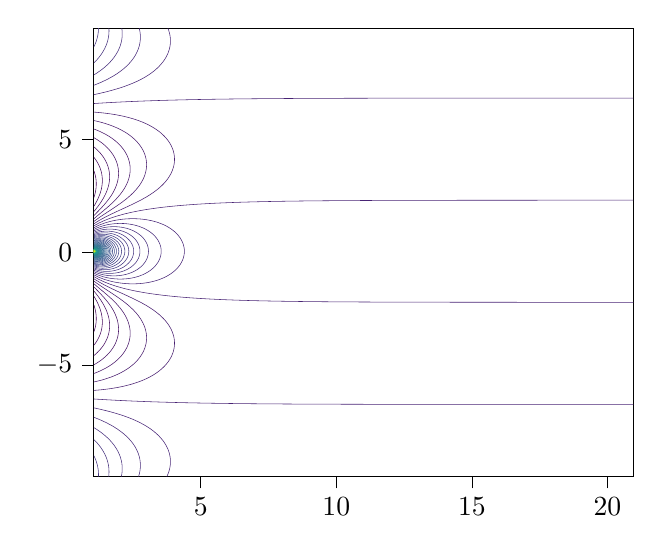
\begin{tikzpicture}

\definecolor{color0}{rgb}{0.271305,0.019942,0.347269}
\definecolor{color1}{rgb}{0.274952,0.037752,0.364543}
\definecolor{color2}{rgb}{0.277941,0.056324,0.381191}
\definecolor{color3}{rgb}{0.280267,0.073417,0.397163}
\definecolor{color4}{rgb}{0.281924,0.089666,0.412415}
\definecolor{color5}{rgb}{0.28291,0.105393,0.426902}
\definecolor{color6}{rgb}{0.283229,0.120777,0.440584}
\definecolor{color7}{rgb}{0.282884,0.13592,0.453427}
\definecolor{color8}{rgb}{0.281887,0.150881,0.465405}
\definecolor{color9}{rgb}{0.280255,0.165693,0.476498}
\definecolor{color10}{rgb}{0.278012,0.180367,0.486697}
\definecolor{color11}{rgb}{0.275191,0.194905,0.496005}
\definecolor{color12}{rgb}{0.271828,0.209303,0.504434}
\definecolor{color13}{rgb}{0.267968,0.223549,0.512008}
\definecolor{color14}{rgb}{0.263663,0.237631,0.518762}
\definecolor{color15}{rgb}{0.258965,0.251537,0.524736}
\definecolor{color16}{rgb}{0.253935,0.265254,0.529983}
\definecolor{color17}{rgb}{0.248629,0.278775,0.534556}
\definecolor{color18}{rgb}{0.243113,0.292092,0.538516}
\definecolor{color19}{rgb}{0.237441,0.305202,0.541921}
\definecolor{color20}{rgb}{0.231674,0.318106,0.544834}
\definecolor{color21}{rgb}{0.225863,0.330805,0.547314}
\definecolor{color22}{rgb}{0.220057,0.343307,0.549413}
\definecolor{color23}{rgb}{0.214298,0.355619,0.551184}
\definecolor{color24}{rgb}{0.208623,0.367752,0.552675}
\definecolor{color25}{rgb}{0.203063,0.379716,0.553925}
\definecolor{color26}{rgb}{0.197636,0.391528,0.554969}
\definecolor{color27}{rgb}{0.192357,0.403199,0.555836}
\definecolor{color28}{rgb}{0.187231,0.414746,0.556547}
\definecolor{color29}{rgb}{0.182256,0.426184,0.55712}
\definecolor{color30}{rgb}{0.177423,0.437527,0.557565}
\definecolor{color31}{rgb}{0.172719,0.448791,0.557885}
\definecolor{color32}{rgb}{0.168126,0.459988,0.558082}
\definecolor{color33}{rgb}{0.163625,0.471133,0.558148}
\definecolor{color34}{rgb}{0.159194,0.482237,0.558073}
\definecolor{color35}{rgb}{0.154815,0.493313,0.55784}
\definecolor{color36}{rgb}{0.150476,0.504369,0.55743}
\definecolor{color37}{rgb}{0.14618,0.515413,0.556823}
\definecolor{color38}{rgb}{0.141935,0.526453,0.555991}
\definecolor{color39}{rgb}{0.13777,0.537492,0.554906}
\definecolor{color40}{rgb}{0.133743,0.548535,0.553541}
\definecolor{color41}{rgb}{0.129933,0.559582,0.551864}
\definecolor{color42}{rgb}{0.126453,0.570633,0.549841}
\definecolor{color43}{rgb}{0.123463,0.581687,0.547445}
\definecolor{color44}{rgb}{0.121148,0.592739,0.544641}
\definecolor{color45}{rgb}{0.119738,0.603785,0.5414}
\definecolor{color46}{rgb}{0.119483,0.614817,0.537692}
\definecolor{color47}{rgb}{0.120638,0.625828,0.533488}
\definecolor{color48}{rgb}{0.123444,0.636809,0.528763}
\definecolor{color49}{rgb}{0.128087,0.647749,0.523491}
\definecolor{color50}{rgb}{0.134692,0.658636,0.517649}
\definecolor{color51}{rgb}{0.143303,0.669459,0.511215}
\definecolor{color52}{rgb}{0.153894,0.680203,0.504172}
\definecolor{color53}{rgb}{0.166383,0.690856,0.496502}
\definecolor{color54}{rgb}{0.180653,0.701402,0.488189}
\definecolor{color55}{rgb}{0.196571,0.711827,0.479221}
\definecolor{color56}{rgb}{0.214,0.722114,0.469588}
\definecolor{color57}{rgb}{0.232815,0.732247,0.459277}
\definecolor{color58}{rgb}{0.252899,0.742211,0.448284}
\definecolor{color59}{rgb}{0.274149,0.751988,0.436601}
\definecolor{color60}{rgb}{0.296479,0.761561,0.424223}
\definecolor{color61}{rgb}{0.319809,0.770914,0.411152}
\definecolor{color62}{rgb}{0.344074,0.780029,0.397381}
\definecolor{color63}{rgb}{0.369214,0.788888,0.382914}
\definecolor{color64}{rgb}{0.395174,0.797475,0.367757}
\definecolor{color65}{rgb}{0.421908,0.805774,0.35191}
\definecolor{color66}{rgb}{0.449368,0.813768,0.335384}
\definecolor{color67}{rgb}{0.477504,0.821444,0.318195}
\definecolor{color68}{rgb}{0.506271,0.828786,0.300362}
\definecolor{color69}{rgb}{0.535621,0.835785,0.281908}
\definecolor{color70}{rgb}{0.565498,0.84243,0.262877}
\definecolor{color71}{rgb}{0.595839,0.848717,0.243329}
\definecolor{color72}{rgb}{0.626579,0.854645,0.223353}
\definecolor{color73}{rgb}{0.657642,0.860219,0.203082}
\definecolor{color74}{rgb}{0.688944,0.865448,0.182725}
\definecolor{color75}{rgb}{0.720391,0.87035,0.162603}
\definecolor{color76}{rgb}{0.751884,0.874951,0.143228}
\definecolor{color77}{rgb}{0.783315,0.879285,0.125405}
\definecolor{color78}{rgb}{0.814576,0.883393,0.110347}
\definecolor{color79}{rgb}{0.845561,0.887322,0.099702}
\definecolor{color80}{rgb}{0.876168,0.891125,0.09525}
\definecolor{color81}{rgb}{0.906311,0.894855,0.098125}
\definecolor{color82}{rgb}{0.935904,0.89857,0.108131}
\definecolor{color83}{rgb}{0.964894,0.902323,0.123941}

\begin{axis}[
tick align=outside,
tick pos=left,
x grid style={white!69.0196078431373!black},
xmin=1.06, xmax=20.96,
xtick style={color=black},
y grid style={white!69.0196078431373!black},
ymin=-9.95, ymax=9.95,
ytick style={color=black}
]
\path [draw=color0, very thin]
(axis cs:1.06,-2.33084279544282)
--(axis cs:1.06596415598527,-2.35)
--(axis cs:1.09156672832119,-2.45)
--(axis cs:1.11247128820641,-2.55)
--(axis cs:1.1287315172552,-2.65)
--(axis cs:1.14035252592001,-2.75)
--(axis cs:1.14729352858579,-2.85)
--(axis cs:1.14946901803413,-2.95)
--(axis cs:1.1467485783386,-3.05)
--(axis cs:1.13895539013389,-3.15)
--(axis cs:1.12586340738216,-3.25)
--(axis cs:1.10719311233359,-3.35)
--(axis cs:1.08260567841278,-3.45)
--(axis cs:1.06,-3.52396190003257);

\path [draw=color0, very thin]
(axis cs:1.06,3.62396190003257)
--(axis cs:1.08260567841278,3.55)
--(axis cs:1.10719311233359,3.45)
--(axis cs:1.12586340738216,3.35)
--(axis cs:1.13895539013389,3.25)
--(axis cs:1.1467485783386,3.15)
--(axis cs:1.14946901803413,3.05)
--(axis cs:1.14729352858579,2.95)
--(axis cs:1.14035252592001,2.85)
--(axis cs:1.1287315172552,2.75)
--(axis cs:1.11247128820641,2.65)
--(axis cs:1.09156672832119,2.55)
--(axis cs:1.06596415598527,2.45)
--(axis cs:1.06,2.43084279544282);

\path [draw=color1, very thin]
(axis cs:1.06,-1.94512402462132)
--(axis cs:1.06277515639247,-1.95)
--(axis cs:1.11275425369982,-2.05)
--(axis cs:1.15751289048816,-2.15)
--(axis cs:1.16,-2.15640575993301)
--(axis cs:1.20010342523948,-2.25)
--(axis cs:1.23758308391499,-2.35)
--(axis cs:1.26,-2.4196079915338)
--(axis cs:1.27074760014764,-2.45)
--(axis cs:1.30019371371818,-2.55)
--(axis cs:1.32451914938554,-2.65)
--(axis cs:1.3438769042583,-2.75)
--(axis cs:1.35835007466792,-2.85)
--(axis cs:1.36,-2.86761611688574)
--(axis cs:1.36840981748404,-2.95)
--(axis cs:1.37335576093469,-3.05)
--(axis cs:1.37303307471321,-3.15)
--(axis cs:1.36732258058104,-3.25)
--(axis cs:1.36,-3.31571057185058)
--(axis cs:1.35622423758699,-3.35)
--(axis cs:1.33987876586398,-3.45)
--(axis cs:1.31761462777415,-3.55)
--(axis cs:1.28903635461633,-3.65)
--(axis cs:1.26,-3.73271384934331)
--(axis cs:1.2539079830586,-3.75)
--(axis cs:1.21274149672585,-3.85)
--(axis cs:1.16371280040037,-3.95)
--(axis cs:1.16,-3.95673740781451)
--(axis cs:1.10778316404305,-4.05)
--(axis cs:1.06,-4.12422617803139);

\path [draw=color1, very thin]
(axis cs:1.06,4.22422617803139)
--(axis cs:1.10778316404305,4.15)
--(axis cs:1.16,4.05673740781451)
--(axis cs:1.16371280040037,4.05)
--(axis cs:1.21274149672585,3.95)
--(axis cs:1.2539079830586,3.85)
--(axis cs:1.26,3.83271384934331)
--(axis cs:1.28903635461633,3.75)
--(axis cs:1.31761462777415,3.65)
--(axis cs:1.33987876586398,3.55)
--(axis cs:1.35622423758699,3.45)
--(axis cs:1.36,3.41571057185058)
--(axis cs:1.36732258058104,3.35)
--(axis cs:1.37303307471321,3.25)
--(axis cs:1.37335576093469,3.15)
--(axis cs:1.36840981748404,3.05)
--(axis cs:1.36,2.96761611688574)
--(axis cs:1.35835007466792,2.95)
--(axis cs:1.3438769042583,2.85)
--(axis cs:1.32451914938554,2.75)
--(axis cs:1.30019371371818,2.65)
--(axis cs:1.27074760014764,2.55)
--(axis cs:1.26,2.5196079915338)
--(axis cs:1.23758308391499,2.45)
--(axis cs:1.20010342523948,2.35)
--(axis cs:1.16,2.25640575993301)
--(axis cs:1.15751289048816,2.25)
--(axis cs:1.11275425369982,2.15)
--(axis cs:1.06277515639247,2.05)
--(axis cs:1.06,2.04512402462132);

\path [draw=color2, very thin]
(axis cs:1.06,-1.71169624804311)
--(axis cs:1.08779794432482,-1.75)
--(axis cs:1.15286996472351,-1.85)
--(axis cs:1.16,-1.86230457440359)
--(axis cs:1.21669914538333,-1.95)
--(axis cs:1.26,-2.02502809961443)
--(axis cs:1.27600753631156,-2.05)
--(axis cs:1.3324116741742,-2.15)
--(axis cs:1.36,-2.20548128784433)
--(axis cs:1.38441214831725,-2.25)
--(axis cs:1.43221355883815,-2.35)
--(axis cs:1.46,-2.41686065435539)
--(axis cs:1.47510667750891,-2.45)
--(axis cs:1.51398444529078,-2.55)
--(axis cs:1.54708885238523,-2.65)
--(axis cs:1.56,-2.69718097292728)
--(axis cs:1.57577532351528,-2.75)
--(axis cs:1.59969381140621,-2.85)
--(axis cs:1.61816104816874,-2.95)
--(axis cs:1.63131815633434,-3.05)
--(axis cs:1.63922389788341,-3.15)
--(axis cs:1.64186308665875,-3.25)
--(axis cs:1.63915127368056,-3.35)
--(axis cs:1.6309363444797,-3.45)
--(axis cs:1.61699737059494,-3.55)
--(axis cs:1.59704082534818,-3.65)
--(axis cs:1.57069407218405,-3.75)
--(axis cs:1.56,-3.78309799707796)
--(axis cs:1.53843658254382,-3.85)
--(axis cs:1.49943945250724,-3.95)
--(axis cs:1.46,-4.0347354944105)
--(axis cs:1.45284443880531,-4.05)
--(axis cs:1.3992971041149,-4.15)
--(axis cs:1.36,-4.21356002009841)
--(axis cs:1.33709243709579,-4.25)
--(axis cs:1.26583582063631,-4.35)
--(axis cs:1.26,-4.35740505704862)
--(axis cs:1.18506598255088,-4.45)
--(axis cs:1.16,-4.47789116389032)
--(axis cs:1.09301272906758,-4.55)
--(axis cs:1.06,-4.58237353443854);

\path [draw=color2, very thin]
(axis cs:1.06,4.68237353443854)
--(axis cs:1.09301272906758,4.65)
--(axis cs:1.16,4.57789116389032)
--(axis cs:1.18506598255088,4.55)
--(axis cs:1.26,4.45740505704862)
--(axis cs:1.26583582063631,4.45)
--(axis cs:1.33709243709579,4.35)
--(axis cs:1.36,4.31356002009841)
--(axis cs:1.3992971041149,4.25)
--(axis cs:1.45284443880531,4.15)
--(axis cs:1.46,4.13473549441051)
--(axis cs:1.49943945250724,4.05)
--(axis cs:1.53843658254382,3.95)
--(axis cs:1.56,3.88309799707796)
--(axis cs:1.57069407218405,3.85)
--(axis cs:1.59704082534818,3.75)
--(axis cs:1.61699737059494,3.65)
--(axis cs:1.6309363444797,3.55)
--(axis cs:1.63915127368056,3.45)
--(axis cs:1.64186308665875,3.35)
--(axis cs:1.63922389788341,3.25)
--(axis cs:1.63131815633434,3.15)
--(axis cs:1.61816104816874,3.05)
--(axis cs:1.59969381140621,2.95)
--(axis cs:1.57577532351528,2.85)
--(axis cs:1.56,2.79718097292728)
--(axis cs:1.54708885238523,2.75)
--(axis cs:1.51398444529078,2.65)
--(axis cs:1.47510667750891,2.55)
--(axis cs:1.46,2.51686065435539)
--(axis cs:1.43221355883815,2.45)
--(axis cs:1.38441214831725,2.35)
--(axis cs:1.36,2.30548128784433)
--(axis cs:1.3324116741742,2.25)
--(axis cs:1.27600753631156,2.15)
--(axis cs:1.26,2.12502809961443)
--(axis cs:1.21669914538333,2.05)
--(axis cs:1.16,1.9623045744036)
--(axis cs:1.15286996472351,1.95)
--(axis cs:1.08779794432482,1.85)
--(axis cs:1.06,1.81169624804311);

\path [draw=color3, very thin]
(axis cs:1.06,-1.53478942057479)
--(axis cs:1.07388924051761,-1.55)
--(axis cs:1.15563058247643,-1.65)
--(axis cs:1.16,-1.65597372828162)
--(axis cs:1.23756474108114,-1.75)
--(axis cs:1.26,-1.78050340874891)
--(axis cs:1.3172744623578,-1.85)
--(axis cs:1.36,-1.90846096605987)
--(axis cs:1.39380613150297,-1.95)
--(axis cs:1.46,-2.04212398742902)
--(axis cs:1.46626591259624,-2.05)
--(axis cs:1.53614145820609,-2.15)
--(axis cs:1.56,-2.1888670354306)
--(axis cs:1.60125401586996,-2.25)
--(axis cs:1.66,-2.3494961219147)
--(axis cs:1.66032580766601,-2.35)
--(axis cs:1.71642870011502,-2.45)
--(axis cs:1.76,-2.53951571269292)
--(axis cs:1.76556587033705,-2.55)
--(axis cs:1.81094851031609,-2.65)
--(axis cs:1.84963423857319,-2.75)
--(axis cs:1.86,-2.78213530164686)
--(axis cs:1.88380261977235,-2.85)
--(axis cs:1.91246257331101,-2.95)
--(axis cs:1.9352289099365,-3.05)
--(axis cs:1.95236571070178,-3.15)
--(axis cs:1.96,-3.21595787005523)
--(axis cs:1.9642787617458,-3.25)
--(axis cs:1.97089565297279,-3.35)
--(axis cs:1.97174469067171,-3.45)
--(axis cs:1.96675751413382,-3.55)
--(axis cs:1.96,-3.61225733858625)
--(axis cs:1.95599453257429,-3.65)
--(axis cs:1.93962709403035,-3.75)
--(axis cs:1.91696090406577,-3.85)
--(axis cs:1.88756294068397,-3.95)
--(axis cs:1.86,-4.02591027365247)
--(axis cs:1.85129133871288,-4.05)
--(axis cs:1.80856733789128,-4.15)
--(axis cs:1.76,-4.24505400316397)
--(axis cs:1.75745852019421,-4.25)
--(axis cs:1.69912341730725,-4.35)
--(axis cs:1.66,-4.40821744238154)
--(axis cs:1.63147231125058,-4.45)
--(axis cs:1.56,-4.54233800516544)
--(axis cs:1.55393461878834,-4.55)
--(axis cs:1.46584268726237,-4.65)
--(axis cs:1.46,-4.65601070364744)
--(axis cs:1.36548870350257,-4.75)
--(axis cs:1.36,-4.75497784024024)
--(axis cs:1.26,-4.8424584668775)
--(axis cs:1.25101956735405,-4.85)
--(axis cs:1.16,-4.92055767642662)
--(axis cs:1.11996417090938,-4.95)
--(axis cs:1.06,-4.99100998531873);

\path [draw=color3, very thin]
(axis cs:1.06,5.09100998531873)
--(axis cs:1.11996417090938,5.05)
--(axis cs:1.16,5.02055767642662)
--(axis cs:1.25101956735405,4.95)
--(axis cs:1.26,4.9424584668775)
--(axis cs:1.36,4.85497784024025)
--(axis cs:1.36548870350257,4.85)
--(axis cs:1.46,4.75601070364744)
--(axis cs:1.46584268726237,4.75)
--(axis cs:1.55393461878834,4.65)
--(axis cs:1.56,4.64233800516544)
--(axis cs:1.63147231125058,4.55)
--(axis cs:1.66,4.50821744238154)
--(axis cs:1.69912341730725,4.45)
--(axis cs:1.75745852019421,4.35)
--(axis cs:1.76,4.34505400316397)
--(axis cs:1.80856733789128,4.25)
--(axis cs:1.85129133871288,4.15)
--(axis cs:1.86,4.12591027365247)
--(axis cs:1.88756294068397,4.05)
--(axis cs:1.91696090406577,3.95)
--(axis cs:1.93962709403035,3.85)
--(axis cs:1.95599453257429,3.75)
--(axis cs:1.96,3.71225733858625)
--(axis cs:1.96675751413382,3.65)
--(axis cs:1.97174469067171,3.55)
--(axis cs:1.97089565297279,3.45)
--(axis cs:1.9642787617458,3.35)
--(axis cs:1.96,3.31595787005523)
--(axis cs:1.95236571070178,3.25)
--(axis cs:1.9352289099365,3.15)
--(axis cs:1.91246257331101,3.05)
--(axis cs:1.88380261977235,2.95)
--(axis cs:1.86,2.88213530164686)
--(axis cs:1.84963423857319,2.85)
--(axis cs:1.81094851031609,2.75)
--(axis cs:1.76556587033705,2.65)
--(axis cs:1.76,2.63951571269292)
--(axis cs:1.71642870011502,2.55)
--(axis cs:1.66032580766601,2.45)
--(axis cs:1.66,2.4494961219147)
--(axis cs:1.60125401586996,2.35)
--(axis cs:1.56,2.2888670354306)
--(axis cs:1.53614145820609,2.25)
--(axis cs:1.46626591259624,2.15)
--(axis cs:1.46,2.14212398742903)
--(axis cs:1.39380613150297,2.05)
--(axis cs:1.36,2.00846096605987)
--(axis cs:1.3172744623578,1.95)
--(axis cs:1.26,1.88050340874891)
--(axis cs:1.23756474108114,1.85)
--(axis cs:1.16,1.75597372828162)
--(axis cs:1.15563058247643,1.75)
--(axis cs:1.07388924051761,1.65)
--(axis cs:1.06,1.63478942057479);

\path [draw=color4, very thin]
(axis cs:1.06,-1.3929359770067)
--(axis cs:1.11839459817286,-1.45)
--(axis cs:1.16,-1.49549037814187)
--(axis cs:1.21709013848871,-1.55)
--(axis cs:1.26,-1.59614739427766)
--(axis cs:1.31679698900697,-1.65)
--(axis cs:1.36,-1.69635287168859)
--(axis cs:1.41620310491116,-1.75)
--(axis cs:1.46,-1.79746179889566)
--(axis cs:1.51404777274753,-1.85)
--(axis cs:1.56,-1.90084088061358)
--(axis cs:1.60917555005076,-1.95)
--(axis cs:1.66,-2.00795032190726)
--(axis cs:1.7005612373382,-2.05)
--(axis cs:1.76,-2.12042256491158)
--(axis cs:1.78731134358089,-2.15)
--(axis cs:1.86,-2.24015057516975)
--(axis cs:1.86864978318579,-2.25)
--(axis cs:1.94532800080549,-2.35)
--(axis cs:1.96,-2.3719844085966)
--(axis cs:2.0165213165374,-2.45)
--(axis cs:2.06,-2.51929009700043)
--(axis cs:2.08086448142016,-2.55)
--(axis cs:2.13955942837414,-2.65)
--(axis cs:2.16,-2.69054522550826)
--(axis cs:2.1924109957809,-2.75)
--(axis cs:2.23883227826831,-2.85)
--(axis cs:2.26,-2.90410173833923)
--(axis cs:2.27940692229577,-2.95)
--(axis cs:2.31442652375747,-3.05)
--(axis cs:2.34285602091485,-3.15)
--(axis cs:2.36,-3.22712332059187)
--(axis cs:2.36550035478466,-3.25)
--(axis cs:2.38303169917047,-3.35)
--(axis cs:2.3944836702456,-3.45)
--(axis cs:2.39998354758793,-3.55)
--(axis cs:2.39955137548267,-3.65)
--(axis cs:2.39310782033926,-3.75)
--(axis cs:2.38047690638681,-3.85)
--(axis cs:2.36138416882773,-3.95)
--(axis cs:2.36,-3.95550692455774)
--(axis cs:2.33667613194538,-4.05)
--(axis cs:2.30499160621597,-4.15)
--(axis cs:2.26563913187152,-4.25)
--(axis cs:2.26,-4.26225084391978)
--(axis cs:2.21974683242482,-4.35)
--(axis cs:2.16502822989394,-4.45)
--(axis cs:2.16,-4.45810448796904)
--(axis cs:2.10256546041672,-4.55)
--(axis cs:2.06,-4.60916872565686)
--(axis cs:2.03020793142219,-4.65)
--(axis cs:1.96,-4.73498816566825)
--(axis cs:1.94733326107514,-4.75)
--(axis cs:1.86,-4.84265602203531)
--(axis cs:1.85287705811341,-4.85)
--(axis cs:1.76,-4.93669240590078)
--(axis cs:1.74521270210074,-4.95)
--(axis cs:1.66,-5.02008995761494)
--(axis cs:1.62195741638073,-5.05)
--(axis cs:1.56,-5.09488978453767)
--(axis cs:1.47965928293708,-5.15)
--(axis cs:1.46,-5.16251641470745)
--(axis cs:1.36,-5.22364486374606)
--(axis cs:1.31432805477815,-5.25)
--(axis cs:1.26,-5.27934621446252)
--(axis cs:1.16,-5.33019710129596)
--(axis cs:1.11881289397079,-5.35)
--(axis cs:1.06,-5.37666681905067);

\path [draw=color4, very thin]
(axis cs:1.06,5.47666681905067)
--(axis cs:1.11881289397079,5.45)
--(axis cs:1.16,5.43019710129597)
--(axis cs:1.26,5.37934621446252)
--(axis cs:1.31432805477815,5.35)
--(axis cs:1.36,5.32364486374606)
--(axis cs:1.46,5.26251641470745)
--(axis cs:1.47965928293708,5.25)
--(axis cs:1.56,5.19488978453767)
--(axis cs:1.62195741638073,5.15)
--(axis cs:1.66,5.12008995761494)
--(axis cs:1.74521270210074,5.05)
--(axis cs:1.76,5.03669240590078)
--(axis cs:1.85287705811341,4.95)
--(axis cs:1.86,4.94265602203531)
--(axis cs:1.94733326107514,4.85)
--(axis cs:1.96,4.83498816566825)
--(axis cs:2.03020793142219,4.75)
--(axis cs:2.06,4.70916872565687)
--(axis cs:2.10256546041672,4.65)
--(axis cs:2.16,4.55810448796904)
--(axis cs:2.16502822989394,4.55)
--(axis cs:2.21974683242482,4.45)
--(axis cs:2.26,4.36225084391979)
--(axis cs:2.26563913187152,4.35)
--(axis cs:2.30499160621597,4.25)
--(axis cs:2.33667613194538,4.15)
--(axis cs:2.36,4.05550692455774)
--(axis cs:2.36138416882773,4.05)
--(axis cs:2.38047690638681,3.95)
--(axis cs:2.39310782033927,3.85)
--(axis cs:2.39955137548267,3.75)
--(axis cs:2.39998354758793,3.65)
--(axis cs:2.3944836702456,3.55)
--(axis cs:2.38303169917047,3.45)
--(axis cs:2.36550035478466,3.35)
--(axis cs:2.36,3.32712332059187)
--(axis cs:2.34285602091485,3.25)
--(axis cs:2.31442652375747,3.15)
--(axis cs:2.27940692229577,3.05)
--(axis cs:2.26,3.00410173833923)
--(axis cs:2.23883227826831,2.95)
--(axis cs:2.1924109957809,2.85)
--(axis cs:2.16,2.79054522550826)
--(axis cs:2.13955942837414,2.75)
--(axis cs:2.08086448142016,2.65)
--(axis cs:2.06,2.61929009700043)
--(axis cs:2.0165213165374,2.55)
--(axis cs:1.96,2.4719844085966)
--(axis cs:1.94532800080549,2.45)
--(axis cs:1.86864978318579,2.35)
--(axis cs:1.86,2.34015057516975)
--(axis cs:1.78731134358088,2.25)
--(axis cs:1.76,2.22042256491158)
--(axis cs:1.7005612373382,2.15)
--(axis cs:1.66,2.10795032190726)
--(axis cs:1.60917555005076,2.05)
--(axis cs:1.56,2.00084088061359)
--(axis cs:1.51404777274753,1.95)
--(axis cs:1.46,1.89746179889566)
--(axis cs:1.41620310491116,1.85)
--(axis cs:1.36,1.7963528716886)
--(axis cs:1.31679698900697,1.75)
--(axis cs:1.26,1.69614739427766)
--(axis cs:1.21709013848871,1.65)
--(axis cs:1.16,1.59549037814187)
--(axis cs:1.11839459817286,1.55)
--(axis cs:1.06,1.4929359770067);

\path [draw=color5, very thin]
(axis cs:1.06,-1.27227399337319)
--(axis cs:1.14926719490279,-1.35)
--(axis cs:1.16,-1.36049169545871)
--(axis cs:1.26,-1.44498736896071)
--(axis cs:1.26684963942243,-1.45)
--(axis cs:1.36,-1.52766713924259)
--(axis cs:1.39050032174684,-1.55)
--(axis cs:1.46,-1.60809893711637)
--(axis cs:1.51638010614844,-1.65)
--(axis cs:1.56,-1.6870511669879)
--(axis cs:1.6424835134609,-1.75)
--(axis cs:1.66,-1.76528808392427)
--(axis cs:1.76,-1.84423194135964)
--(axis cs:1.76804890102753,-1.85)
--(axis cs:1.86,-1.92549376448958)
--(axis cs:1.89245906010955,-1.95)
--(axis cs:1.96,-2.00841948268148)
--(axis cs:2.01199303030904,-2.05)
--(axis cs:2.06,-2.09399800839553)
--(axis cs:2.12580818250535,-2.15)
--(axis cs:2.16,-2.18336872360946)
--(axis cs:2.23329182605818,-2.25)
--(axis cs:2.26,-2.27787869857636)
--(axis cs:2.3339894388333,-2.35)
--(axis cs:2.36,-2.37916010577231)
--(axis cs:2.42754562923735,-2.45)
--(axis cs:2.46,-2.48923705529328)
--(axis cs:2.51365752982693,-2.55)
--(axis cs:2.56,-2.61067640084866)
--(axis cs:2.59203867132987,-2.65)
--(axis cs:2.66,-2.74680594415809)
--(axis cs:2.66239093934491,-2.75)
--(axis cs:2.72718543050768,-2.85)
--(axis cs:2.76,-2.90945582244773)
--(axis cs:2.78391925640058,-2.95)
--(axis cs:2.8340149915479,-3.05)
--(axis cs:2.86,-3.11186311589148)
--(axis cs:2.87716317056172,-3.15)
--(axis cs:2.91437500992477,-3.25)
--(axis cs:2.94439613098192,-3.35)
--(axis cs:2.96,-3.41677580718998)
--(axis cs:2.96835339213981,-3.45)
--(axis cs:2.98670609375547,-3.55)
--(axis cs:2.99864597554046,-3.65)
--(axis cs:3.00434907965498,-3.75)
--(axis cs:3.00386666630186,-3.85)
--(axis cs:2.99713464235223,-3.95)
--(axis cs:2.98397674904834,-4.05)
--(axis cs:2.96410210117403,-4.15)
--(axis cs:2.96,-4.16559001054174)
--(axis cs:2.93831812715565,-4.25)
--(axis cs:2.9054144019583,-4.35)
--(axis cs:2.86447315643955,-4.45)
--(axis cs:2.86,-4.4593195337411)
--(axis cs:2.81684565933803,-4.55)
--(axis cs:2.76,-4.64968211855395)
--(axis cs:2.75981905134229,-4.65)
--(axis cs:2.69494574829709,-4.75)
--(axis cs:2.66,-4.79670154357411)
--(axis cs:2.61971349293793,-4.85)
--(axis cs:2.56,-4.91955262106258)
--(axis cs:2.53339595091744,-4.95)
--(axis cs:2.46,-5.02490835574774)
--(axis cs:2.43477772073929,-5.05)
--(axis cs:2.36,-5.11706108324366)
--(axis cs:2.32199047821964,-5.15)
--(axis cs:2.26,-5.198879342637)
--(axis cs:2.19226078231984,-5.25)
--(axis cs:2.16,-5.27233160669999)
--(axis cs:2.06,-5.33857087547647)
--(axis cs:2.04207637982084,-5.35)
--(axis cs:1.96,-5.39844908690815)
--(axis cs:1.86633195911756,-5.45)
--(axis cs:1.86,-5.453245871538)
--(axis cs:1.76,-5.50296267116754)
--(axis cs:1.66,-5.54869388677691)
--(axis cs:1.65704791968238,-5.55)
--(axis cs:1.56,-5.59035745709938)
--(axis cs:1.46,-5.62866072840581)
--(axis cs:1.40055261462096,-5.65)
--(axis cs:1.36,-5.66376916263108)
--(axis cs:1.26,-5.69590553564647)
--(axis cs:1.16,-5.72537394784684)
--(axis cs:1.06906759277243,-5.75)
--(axis cs:1.06,-5.75233952088003);

\path [draw=color5, very thin]
(axis cs:1.06,5.85233952088003)
--(axis cs:1.06906759277243,5.85)
--(axis cs:1.16,5.82537394784684)
--(axis cs:1.26,5.79590553564647)
--(axis cs:1.36,5.76376916263108)
--(axis cs:1.40055261462096,5.75)
--(axis cs:1.46,5.72866072840581)
--(axis cs:1.56,5.69035745709938)
--(axis cs:1.65704791968238,5.65)
--(axis cs:1.66,5.64869388677691)
--(axis cs:1.76,5.60296267116754)
--(axis cs:1.86,5.553245871538)
--(axis cs:1.86633195911756,5.55)
--(axis cs:1.96,5.49844908690815)
--(axis cs:2.04207637982084,5.45)
--(axis cs:2.06,5.43857087547647)
--(axis cs:2.16,5.37233160669999)
--(axis cs:2.19226078231983,5.35)
--(axis cs:2.26,5.298879342637)
--(axis cs:2.32199047821964,5.25)
--(axis cs:2.36,5.21706108324366)
--(axis cs:2.43477772073929,5.15)
--(axis cs:2.46,5.12490835574774)
--(axis cs:2.53339595091744,5.05)
--(axis cs:2.56,5.01955262106258)
--(axis cs:2.61971349293793,4.95)
--(axis cs:2.66,4.89670154357411)
--(axis cs:2.69494574829709,4.85)
--(axis cs:2.75981905134229,4.75)
--(axis cs:2.76,4.74968211855395)
--(axis cs:2.81684565933803,4.65)
--(axis cs:2.86,4.5593195337411)
--(axis cs:2.86447315643955,4.55)
--(axis cs:2.9054144019583,4.45)
--(axis cs:2.93831812715565,4.35)
--(axis cs:2.96,4.26559001054174)
--(axis cs:2.96410210117403,4.25)
--(axis cs:2.98397674904834,4.15)
--(axis cs:2.99713464235223,4.05)
--(axis cs:3.00386666630186,3.95)
--(axis cs:3.00434907965498,3.85)
--(axis cs:2.99864597554046,3.75)
--(axis cs:2.98670609375547,3.65)
--(axis cs:2.96835339213981,3.55)
--(axis cs:2.96,3.51677580718998)
--(axis cs:2.94439613098192,3.45)
--(axis cs:2.91437500992477,3.35)
--(axis cs:2.87716317056172,3.25)
--(axis cs:2.86,3.21186311589148)
--(axis cs:2.8340149915479,3.15)
--(axis cs:2.78391925640058,3.05)
--(axis cs:2.76,3.00945582244773)
--(axis cs:2.72718543050768,2.95)
--(axis cs:2.66239093934491,2.85)
--(axis cs:2.66,2.84680594415808)
--(axis cs:2.59203867132987,2.75)
--(axis cs:2.56,2.71067640084866)
--(axis cs:2.51365752982693,2.65)
--(axis cs:2.46,2.58923705529328)
--(axis cs:2.42754562923735,2.55)
--(axis cs:2.36,2.47916010577231)
--(axis cs:2.3339894388333,2.45)
--(axis cs:2.26,2.37787869857636)
--(axis cs:2.23329182605818,2.35)
--(axis cs:2.16,2.28336872360946)
--(axis cs:2.12580818250535,2.25)
--(axis cs:2.06,2.19399800839553)
--(axis cs:2.01199303030904,2.15)
--(axis cs:1.96,2.10841948268148)
--(axis cs:1.89245906010955,2.05)
--(axis cs:1.86,2.02549376448958)
--(axis cs:1.76804890102753,1.95)
--(axis cs:1.76,1.94423194135964)
--(axis cs:1.66,1.86528808392427)
--(axis cs:1.6424835134609,1.85)
--(axis cs:1.56,1.7870511669879)
--(axis cs:1.51638010614844,1.75)
--(axis cs:1.46,1.70809893711637)
--(axis cs:1.39050032174684,1.65)
--(axis cs:1.36,1.62766713924259)
--(axis cs:1.26684963942243,1.55)
--(axis cs:1.26,1.54498736896071)
--(axis cs:1.16,1.46049169545872)
--(axis cs:1.14926719490279,1.45)
--(axis cs:1.06,1.3722739933732);

\path [draw=color6, very thin]
(axis cs:1.06,-1.16820653608664)
--(axis cs:1.16,-1.2455679977991)
--(axis cs:1.16680999574596,-1.25)
--(axis cs:1.26,-1.31921834056765)
--(axis cs:1.3084244614847,-1.35)
--(axis cs:1.36,-1.3875374643957)
--(axis cs:1.45856002529588,-1.45)
--(axis cs:1.46,-1.45104620241209)
--(axis cs:1.56,-1.51416715787026)
--(axis cs:1.6236124053371,-1.55)
--(axis cs:1.66,-1.573571892908)
--(axis cs:1.76,-1.63139512457812)
--(axis cs:1.79575947280412,-1.65)
--(axis cs:1.86,-1.68841932222631)
--(axis cs:1.96,-1.74339821649188)
--(axis cs:1.9732825624669,-1.75)
--(axis cs:2.06,-1.79944279893676)
--(axis cs:2.15409684481289,-1.85)
--(axis cs:2.16,-1.85363326935073)
--(axis cs:2.26,-1.9097519144234)
--(axis cs:2.33522970041728,-1.95)
--(axis cs:2.36,-1.96515012747817)
--(axis cs:2.46,-2.02219268912877)
--(axis cs:2.51115781370383,-2.05)
--(axis cs:2.56,-2.08029665239344)
--(axis cs:2.66,-2.13962610465381)
--(axis cs:2.67848393466857,-2.15)
--(axis cs:2.76,-2.20213902622583)
--(axis cs:2.83701579721689,-2.25)
--(axis cs:2.86,-2.26629167774108)
--(axis cs:2.96,-2.33406574644946)
--(axis cs:2.98444620149635,-2.35)
--(axis cs:3.06,-2.40616128304455)
--(axis cs:3.12072445806228,-2.45)
--(axis cs:3.16,-2.48239947987196)
--(axis cs:3.24468959977905,-2.55)
--(axis cs:3.26,-2.56400051153028)
--(axis cs:3.35751984126944,-2.65)
--(axis cs:3.36,-2.65251371844429)
--(axis cs:3.46,-2.74995288746252)
--(axis cs:3.46005017173883,-2.75)
--(axis cs:3.55282514031685,-2.85)
--(axis cs:3.56,-2.85896623797613)
--(axis cs:3.63619197869248,-2.95)
--(axis cs:3.66,-2.98317328465886)
--(axis cs:3.71029181263143,-3.05)
--(axis cs:3.76,-3.12757723820136)
--(axis cs:3.7751028447761,-3.15)
--(axis cs:3.83261219117443,-3.25)
--(axis cs:3.86,-3.30681845973511)
--(axis cs:3.88202028013173,-3.35)
--(axis cs:3.92441321099153,-3.45)
--(axis cs:3.95872851981216,-3.55)
--(axis cs:3.96,-3.5546825497747)
--(axis cs:3.98762231557991,-3.65)
--(axis cs:4.00935728480756,-3.75)
--(axis cs:4.02429445725531,-3.85)
--(axis cs:4.03271751409403,-3.95)
--(axis cs:4.03476206896461,-4.05)
--(axis cs:4.03042890688643,-4.15)
--(axis cs:4.01958942116643,-4.25)
--(axis cs:4.00198404457561,-4.35)
--(axis cs:3.97721374771833,-4.45)
--(axis cs:3.96,-4.50373091331504)
--(axis cs:3.94559525477758,-4.55)
--(axis cs:3.90693651552363,-4.65)
--(axis cs:3.86,-4.74862972069538)
--(axis cs:3.85935903089997,-4.75)
--(axis cs:3.80472349419868,-4.85)
--(axis cs:3.76,-4.91907674449764)
--(axis cs:3.74008015358933,-4.95)
--(axis cs:3.66541696195458,-5.05)
--(axis cs:3.66,-5.05641085348816)
--(axis cs:3.58025034735984,-5.15)
--(axis cs:3.56,-5.17095530269272)
--(axis cs:3.48231622769778,-5.25)
--(axis cs:3.46,-5.27024411002661)
--(axis cs:3.36975515476929,-5.35)
--(axis cs:3.36,-5.35775939041867)
--(axis cs:3.26,-5.43542400283297)
--(axis cs:3.24061786161228,-5.45)
--(axis cs:3.16,-5.5051166804661)
--(axis cs:3.09095396851874,-5.55)
--(axis cs:3.06,-5.56842572484116)
--(axis cs:2.96,-5.62574826563131)
--(axis cs:2.91560239240367,-5.65)
--(axis cs:2.86,-5.67803665974041)
--(axis cs:2.76,-5.72583840624636)
--(axis cs:2.70662882568454,-5.75)
--(axis cs:2.66,-5.76962750716126)
--(axis cs:2.56,-5.80969366403389)
--(axis cs:2.46,-5.84662648335386)
--(axis cs:2.4505635376018,-5.85)
--(axis cs:2.36,-5.88034394245665)
--(axis cs:2.26,-5.91136145569265)
--(axis cs:2.16,-5.93987939863457)
--(axis cs:2.12257958377392,-5.95)
--(axis cs:2.06,-5.96597753170045)
--(axis cs:1.96,-5.98986639451303)
--(axis cs:1.86,-6.01172927456146)
--(axis cs:1.76,-6.03168590130872)
--(axis cs:1.66,-6.04984763197513)
--(axis cs:1.6591187348728,-6.05)
--(axis cs:1.56,-6.06632500882678)
--(axis cs:1.46,-6.08122465232346)
--(axis cs:1.36,-6.0946327918192)
--(axis cs:1.26,-6.10662946284685)
--(axis cs:1.16,-6.11728892999269)
--(axis cs:1.06,-6.12668006002559);

\path [draw=color6, very thin]
(axis cs:1.06,6.22668006002559)
--(axis cs:1.16,6.2172889299927)
--(axis cs:1.26,6.20662946284685)
--(axis cs:1.36,6.1946327918192)
--(axis cs:1.46,6.18122465232346)
--(axis cs:1.56,6.16632500882678)
--(axis cs:1.65911873487279,6.15)
--(axis cs:1.66,6.14984763197513)
--(axis cs:1.76,6.13168590130873)
--(axis cs:1.86,6.11172927456146)
--(axis cs:1.96,6.08986639451303)
--(axis cs:2.06,6.06597753170045)
--(axis cs:2.12257958377392,6.05)
--(axis cs:2.16,6.03987939863457)
--(axis cs:2.26,6.01136145569265)
--(axis cs:2.36,5.98034394245665)
--(axis cs:2.4505635376018,5.95)
--(axis cs:2.46,5.94662648335386)
--(axis cs:2.56,5.9096936640339)
--(axis cs:2.66,5.86962750716126)
--(axis cs:2.70662882568453,5.85)
--(axis cs:2.76,5.82583840624636)
--(axis cs:2.86,5.77803665974041)
--(axis cs:2.91560239240367,5.75)
--(axis cs:2.96,5.72574826563131)
--(axis cs:3.06,5.66842572484116)
--(axis cs:3.09095396851874,5.65)
--(axis cs:3.16,5.6051166804661)
--(axis cs:3.24061786161228,5.55)
--(axis cs:3.26,5.53542400283297)
--(axis cs:3.36,5.45775939041867)
--(axis cs:3.36975515476929,5.45)
--(axis cs:3.46,5.37024411002661)
--(axis cs:3.48231622769778,5.35)
--(axis cs:3.56,5.27095530269272)
--(axis cs:3.58025034735984,5.25)
--(axis cs:3.66,5.15641085348816)
--(axis cs:3.66541696195458,5.15)
--(axis cs:3.74008015358933,5.05)
--(axis cs:3.76,5.01907674449764)
--(axis cs:3.80472349419868,4.95)
--(axis cs:3.85935903089996,4.85)
--(axis cs:3.86,4.84862972069537)
--(axis cs:3.90693651552363,4.75)
--(axis cs:3.94559525477758,4.65)
--(axis cs:3.96,4.60373091331504)
--(axis cs:3.97721374771833,4.55)
--(axis cs:4.00198404457561,4.45)
--(axis cs:4.01958942116643,4.35)
--(axis cs:4.03042890688643,4.25)
--(axis cs:4.03476206896461,4.15)
--(axis cs:4.03271751409403,4.05)
--(axis cs:4.02429445725531,3.95)
--(axis cs:4.00935728480756,3.85)
--(axis cs:3.98762231557991,3.75)
--(axis cs:3.96,3.6546825497747)
--(axis cs:3.95872851981216,3.65)
--(axis cs:3.92441321099153,3.55)
--(axis cs:3.88202028013173,3.45)
--(axis cs:3.86,3.40681845973511)
--(axis cs:3.83261219117443,3.35)
--(axis cs:3.7751028447761,3.25)
--(axis cs:3.76,3.22757723820136)
--(axis cs:3.71029181263143,3.15)
--(axis cs:3.66,3.08317328465886)
--(axis cs:3.63619197869248,3.05)
--(axis cs:3.56,2.95896623797614)
--(axis cs:3.55282514031685,2.95)
--(axis cs:3.46005017173883,2.85)
--(axis cs:3.46,2.84995288746252)
--(axis cs:3.36,2.75251371844429)
--(axis cs:3.35751984126944,2.75)
--(axis cs:3.26,2.66400051153028)
--(axis cs:3.24468959977905,2.65)
--(axis cs:3.16,2.58239947987196)
--(axis cs:3.12072445806228,2.55)
--(axis cs:3.06,2.50616128304455)
--(axis cs:2.98444620149635,2.45)
--(axis cs:2.96,2.43406574644946)
--(axis cs:2.86,2.36629167774108)
--(axis cs:2.83701579721689,2.35)
--(axis cs:2.76,2.30213902622583)
--(axis cs:2.67848393466857,2.25)
--(axis cs:2.66,2.23962610465381)
--(axis cs:2.56,2.18029665239344)
--(axis cs:2.51115781370383,2.15)
--(axis cs:2.46,2.12219268912877)
--(axis cs:2.36,2.06515012747817)
--(axis cs:2.33522970041728,2.05)
--(axis cs:2.26,2.00975191442341)
--(axis cs:2.16,1.95363326935074)
--(axis cs:2.15409684481289,1.95)
--(axis cs:2.06,1.89944279893676)
--(axis cs:1.9732825624669,1.85)
--(axis cs:1.96,1.84339821649188)
--(axis cs:1.86,1.78841932222631)
--(axis cs:1.79575947280412,1.75)
--(axis cs:1.76,1.73139512457812)
--(axis cs:1.66,1.673571892908)
--(axis cs:1.6236124053371,1.65)
--(axis cs:1.56,1.61416715787026)
--(axis cs:1.46,1.55104620241209)
--(axis cs:1.45856002529588,1.55)
--(axis cs:1.36,1.4875374643957)
--(axis cs:1.3084244614847,1.45)
--(axis cs:1.26,1.41921834056765)
--(axis cs:1.16680999574596,1.35)
--(axis cs:1.16,1.3455679977991)
--(axis cs:1.06,1.26820653608664);

\path [draw=color7, very thin]
(axis cs:20.96,-6.7484266811197)
--(axis cs:20.86,-6.74842203914304)
--(axis cs:20.76,-6.74841720574146)
--(axis cs:20.66,-6.7484121733673)
--(axis cs:20.56,-6.74840693330744)
--(axis cs:20.46,-6.74840147734465)
--(axis cs:20.36,-6.74839579615312)
--(axis cs:20.26,-6.74838988097475)
--(axis cs:20.16,-6.74838372242004)
--(axis cs:20.06,-6.74837731005904)
--(axis cs:19.96,-6.74837063310798)
--(axis cs:19.86,-6.74836368153492)
--(axis cs:19.76,-6.7483564432568)
--(axis cs:19.66,-6.74834890706021)
--(axis cs:19.56,-6.74834106030647)
--(axis cs:19.46,-6.74833289074221)
--(axis cs:19.36,-6.74832438491001)
--(axis cs:19.26,-6.7483155289229)
--(axis cs:19.16,-6.74830630843229)
--(axis cs:19.06,-6.74829670839315)
--(axis cs:18.96,-6.74828671363413)
--(axis cs:18.86,-6.74827630748486)
--(axis cs:18.76,-6.74826547338988)
--(axis cs:18.66,-6.74825419376254)
--(axis cs:18.56,-6.74824245042085)
--(axis cs:18.46,-6.74823022427762)
--(axis cs:18.36,-6.74821749565261)
--(axis cs:18.26,-6.74820424384073)
--(axis cs:18.16,-6.74819044756869)
--(axis cs:18.06,-6.74817608458623)
--(axis cs:17.96,-6.74816113167069)
--(axis cs:17.86,-6.7481455647188)
--(axis cs:17.76,-6.74812935867398)
--(axis cs:17.66,-6.74811248741863)
--(axis cs:17.56,-6.7480949237634)
--(axis cs:17.46,-6.74807663951923)
--(axis cs:17.36,-6.74805760525389)
--(axis cs:17.26,-6.74803779038644)
--(axis cs:17.16,-6.74801716308758)
--(axis cs:17.06,-6.74799569024366)
--(axis cs:16.96,-6.74797333740115)
--(axis cs:16.86,-6.74795006883416)
--(axis cs:16.76,-6.74792584716968)
--(axis cs:16.66,-6.74790063362849)
--(axis cs:16.56,-6.74787438798549)
--(axis cs:16.46,-6.74784706813796)
--(axis cs:16.36,-6.74781863054351)
--(axis cs:16.26,-6.74778902982685)
--(axis cs:16.16,-6.74775821873795)
--(axis cs:16.06,-6.74772614813889)
--(axis cs:15.96,-6.74769276706228)
--(axis cs:15.86,-6.74765802231275)
--(axis cs:15.76,-6.74762185871572)
--(axis cs:15.66,-6.74758421878861)
--(axis cs:15.56,-6.74754504281897)
--(axis cs:15.46,-6.74750426871418)
--(axis cs:15.36,-6.74746183186248)
--(axis cs:15.26,-6.74741766511155)
--(axis cs:15.16,-6.74737169864084)
--(axis cs:15.06,-6.74732385987947)
--(axis cs:14.96,-6.74727407331126)
--(axis cs:14.86,-6.74722226049659)
--(axis cs:14.76,-6.74716833984353)
--(axis cs:14.66,-6.74711222657836)
--(axis cs:14.56,-6.74705383254214)
--(axis cs:14.46,-6.74699306609515)
--(axis cs:14.36,-6.74692983201776)
--(axis cs:14.26,-6.7468640313344)
--(axis cs:14.16,-6.74679556115615)
--(axis cs:14.06,-6.74672431457481)
--(axis cs:13.96,-6.74665018049185)
--(axis cs:13.86,-6.74657304345475)
--(axis cs:13.76,-6.74649278348845)
--(axis cs:13.66,-6.74640927595081)
--(axis cs:13.56,-6.7463223913239)
--(axis cs:13.46,-6.74623199504706)
--(axis cs:13.36,-6.74613794734722)
--(axis cs:13.26,-6.74604010300711)
--(axis cs:13.16,-6.74593831118412)
--(axis cs:13.06,-6.74583241520601)
--(axis cs:12.96,-6.74572225234884)
--(axis cs:12.86,-6.74560765359573)
--(axis cs:12.76,-6.74548844344516)
--(axis cs:12.66,-6.74536443963351)
--(axis cs:12.56,-6.74523545290978)
--(axis cs:12.46,-6.74510128677809)
--(axis cs:12.36,-6.74496173722682)
--(axis cs:12.26,-6.74481659246153)
--(axis cs:12.16,-6.74466563262097)
--(axis cs:12.06,-6.74450862949357)
--(axis cs:11.96,-6.74434534620659)
--(axis cs:11.86,-6.74417553692156)
--(axis cs:11.76,-6.74399894651975)
--(axis cs:11.66,-6.74381531026205)
--(axis cs:11.56,-6.74362435345646)
--(axis cs:11.46,-6.74342579110543)
--(axis cs:11.36,-6.74321932754021)
--(axis cs:11.26,-6.7430046560507)
--(axis cs:11.16,-6.74278145850198)
--(axis cs:11.06,-6.74254940493316)
--(axis cs:10.96,-6.74230815315218)
--(axis cs:10.86,-6.74205734831353)
--(axis cs:10.76,-6.74179662248472)
--(axis cs:10.66,-6.74152559419946)
--(axis cs:10.56,-6.74124386799912)
--(axis cs:10.46,-6.74095103395883)
--(axis cs:10.36,-6.74064666720009)
--(axis cs:10.26,-6.74033032739154)
--(axis cs:10.16,-6.74000155823354)
--(axis cs:10.06,-6.7396598869291)
--(axis cs:9.96,-6.7393048236388)
--(axis cs:9.86,-6.73893586092355)
--(axis cs:9.76,-6.73855247316811)
--(axis cs:9.66,-6.73815411599358)
--(axis cs:9.56,-6.73774022565079)
--(axis cs:9.46,-6.73731021839913)
--(axis cs:9.36,-6.73686348986766)
--(axis cs:9.26,-6.73639941440336)
--(axis cs:9.16,-6.73591734439859)
--(axis cs:9.06,-6.73541660960398)
--(axis cs:8.96,-6.73489651642332)
--(axis cs:8.86,-6.73435634719178)
--(axis cs:8.76,-6.73379535943671)
--(axis cs:8.66,-6.73321278511922)
--(axis cs:8.56,-6.73260782986005)
--(axis cs:8.46,-6.73197967214571)
--(axis cs:8.36,-6.73132746251725)
--(axis cs:8.26,-6.73065032274044)
--(axis cs:8.16,-6.72994734495691)
--(axis cs:8.06,-6.72921759081783)
--(axis cs:7.96,-6.7284600905974)
--(axis cs:7.86,-6.7276738422882)
--(axis cs:7.76,-6.72685781067748)
--(axis cs:7.66,-6.72601092640445)
--(axis cs:7.56,-6.72513208499756)
--(axis cs:7.46,-6.72422014589357)
--(axis cs:7.36,-6.72327393143675)
--(axis cs:7.26,-6.72229222585878)
--(axis cs:7.16,-6.72127377423914)
--(axis cs:7.06,-6.72021728144662)
--(axis cs:6.96,-6.71912141106096)
--(axis cs:6.86,-6.71798478427544)
--(axis cs:6.76,-6.71680597878006)
--(axis cs:6.66,-6.715583527626)
--(axis cs:6.56,-6.71431591807049)
--(axis cs:6.46,-6.71300159040343)
--(axis cs:6.36,-6.71163893675509)
--(axis cs:6.26,-6.71022629988556)
--(axis cs:6.16,-6.70876197195643)
--(axis cs:6.06,-6.70724419328464)
--(axis cs:5.96,-6.70567115107943)
--(axis cs:5.86,-6.70404097816273)
--(axis cs:5.76,-6.70235175167374)
--(axis cs:5.66,-6.70060149175847)
--(axis cs:5.56,-6.69878816024524)
--(axis cs:5.46,-6.69690965930697)
--(axis cs:5.36,-6.69496383011184)
--(axis cs:5.26,-6.69294845146351)
--(axis cs:5.16,-6.69086123843242)
--(axis cs:5.06,-6.68869984098041)
--(axis cs:4.96,-6.68646184258024)
--(axis cs:4.86,-6.68414475883284)
--(axis cs:4.76,-6.68174603608458)
--(axis cs:4.66,-6.67926305004777)
--(axis cs:4.56,-6.67669310442765)
--(axis cs:4.46,-6.67403342955942)
--(axis cs:4.36,-6.67128118105967)
--(axis cs:4.26,-6.66843343849636)
--(axis cs:4.16,-6.66548720408256)
--(axis cs:4.06,-6.66243940139912)
--(axis cs:3.96,-6.6592868741522)
--(axis cs:3.86,-6.65602638497192)
--(axis cs:3.76,-6.65265461425888)
--(axis cs:3.68491520388505,-6.65)
--(axis cs:3.66,-6.64917250135341)
--(axis cs:3.56,-6.64558774852738)
--(axis cs:3.46,-6.64188367092179)
--(axis cs:3.36,-6.63805672538805)
--(axis cs:3.26,-6.63410328180696)
--(axis cs:3.16,-6.63001962196165)
--(axis cs:3.06,-6.62580193850029)
--(axis cs:2.96,-6.6214463340014)
--(axis cs:2.86,-6.61694882015517)
--(axis cs:2.76,-6.61230531707471)
--(axis cs:2.66,-6.60751165275161)
--(axis cs:2.56,-6.60256356267023)
--(axis cs:2.46,-6.59745668959554)
--(axis cs:2.36,-6.59218658354931)
--(axis cs:2.26,-6.58674870198912)
--(axis cs:2.16,-6.58113841020476)
--(axis cs:2.06,-6.57535098194587)
--(axis cs:1.96,-6.56938160029435)
--(axis cs:1.86,-6.56322535879415)
--(axis cs:1.76,-6.55687726285058)
--(axis cs:1.66,-6.55033223140995)
--(axis cs:1.65528902706467,-6.55)
--(axis cs:1.56,-6.54363911219931)
--(axis cs:1.46,-6.53674653307891)
--(axis cs:1.36,-6.52964652383321)
--(axis cs:1.26,-6.52233373875368)
--(axis cs:1.16,-6.51480274735818)
--(axis cs:1.06,-6.50704803771116);

\path [draw=color7, very thin]
(axis cs:1.06,-1.07710514456378)
--(axis cs:1.16,-1.14544469607991)
--(axis cs:1.16809389021247,-1.15)
--(axis cs:1.26,-1.20944239222008)
--(axis cs:1.33440382230529,-1.25)
--(axis cs:1.36,-1.26607393567273)
--(axis cs:1.46,-1.31915377372468)
--(axis cs:1.52733390111083,-1.35)
--(axis cs:1.56,-1.36731877888643)
--(axis cs:1.66,-1.41276631037542)
--(axis cs:1.75208284830795,-1.45)
--(axis cs:1.76,-1.45370033869637)
--(axis cs:1.86,-1.49361861620119)
--(axis cs:1.96,-1.52974098273406)
--(axis cs:2.02289302992224,-1.55)
--(axis cs:2.06,-1.56374667892957)
--(axis cs:2.16,-1.59626592253069)
--(axis cs:2.26,-1.62617654588931)
--(axis cs:2.34680292683707,-1.65)
--(axis cs:2.36,-1.65413545299581)
--(axis cs:2.46,-1.68141777374735)
--(axis cs:2.56,-1.70674369742982)
--(axis cs:2.66,-1.73037735013818)
--(axis cs:2.74931678454986,-1.75)
--(axis cs:2.76,-1.75265401447749)
--(axis cs:2.86,-1.77440531935019)
--(axis cs:2.96,-1.79478261672358)
--(axis cs:3.06,-1.81393685789637)
--(axis cs:3.16,-1.83199416680368)
--(axis cs:3.26,-1.84906062403899)
--(axis cs:3.26625027888483,-1.85)
--(axis cs:3.36,-1.86572594218043)
--(axis cs:3.46,-1.88148276496992)
--(axis cs:3.56,-1.89638048550883)
--(axis cs:3.66,-1.91049091210635)
--(axis cs:3.76,-1.92387647007682)
--(axis cs:3.86,-1.93659176505722)
--(axis cs:3.96,-1.94868485717762)
--(axis cs:3.97222017831548,-1.95)
--(axis cs:4.06,-1.96042748090149)
--(axis cs:4.16,-1.97160624328277)
--(axis cs:4.26,-1.98223030010366)
--(axis cs:4.36,-1.99233664580545)
--(axis cs:4.46,-2.00195855897161)
--(axis cs:4.56,-2.01112611283579)
--(axis cs:4.66,-2.01986660335028)
--(axis cs:4.76,-2.02820490930379)
--(axis cs:4.86,-2.03616379627931)
--(axis cs:4.96,-2.04376417407206)
--(axis cs:5.046759237156,-2.05)
--(axis cs:5.06,-2.05103955998175)
--(axis cs:5.16,-2.05806722592477)
--(axis cs:5.26,-2.06477250216215)
--(axis cs:5.36,-2.07117293194888)
--(axis cs:5.46,-2.07728477139809)
--(axis cs:5.56,-2.08312312174141)
--(axis cs:5.66,-2.08870204430755)
--(axis cs:5.76,-2.09403466080465)
--(axis cs:5.86,-2.09913324107145)
--(axis cs:5.96,-2.10400928011597)
--(axis cs:6.06,-2.10867356597185)
--(axis cs:6.16,-2.11313623966323)
--(axis cs:6.26,-2.11740684836965)
--(axis cs:6.36,-2.12149439271533)
--(axis cs:6.46,-2.12540736896871)
--(axis cs:6.56,-2.12915380681997)
--(axis cs:6.66,-2.13274130330707)
--(axis cs:6.76,-2.13617705337762)
--(axis cs:6.86,-2.13946787750397)
--(axis cs:6.96,-2.1426202467104)
--(axis cs:7.06,-2.14564030532065)
--(axis cs:7.16,-2.14853389169229)
--(axis cs:7.21465663794299,-2.15)
--(axis cs:7.26,-2.1513130754581)
--(axis cs:7.36,-2.15398194345721)
--(axis cs:7.46,-2.15653793988821)
--(axis cs:7.56,-2.15898610498809)
--(axis cs:7.66,-2.1613312284099)
--(axis cs:7.76,-2.16357786427717)
--(axis cs:7.86,-2.16573034506906)
--(axis cs:7.96,-2.16779279445109)
--(axis cs:8.06,-2.16976913915509)
--(axis cs:8.16,-2.17166311999841)
--(axis cs:8.26,-2.17347830212295)
--(axis cs:8.36,-2.17521808452473)
--(axis cs:8.46,-2.17688570893833)
--(axis cs:8.56,-2.17848426813054)
--(axis cs:8.66,-2.18001671365676)
--(axis cs:8.76,-2.18148586312126)
--(axis cs:8.86,-2.18289440698475)
--(axis cs:8.96,-2.18424491495452)
--(axis cs:9.06,-2.18553984198868)
--(axis cs:9.16,-2.18678153394643)
--(axis cs:9.26,-2.18797223290781)
--(axis cs:9.36,-2.18911408218988)
--(axis cs:9.46,-2.19020913107982)
--(axis cs:9.56,-2.19125933930458)
--(axis cs:9.66,-2.19226658125602)
--(axis cs:9.76,-2.19323264998757)
--(axis cs:9.86,-2.19415926099854)
--(axis cs:9.96,-2.19504805581738)
--(axis cs:10.06,-2.19590060540023)
--(axis cs:10.16,-2.19671841335357)
--(axis cs:10.26,-2.19750291899222)
--(axis cs:10.36,-2.19825550024525)
--(axis cs:10.46,-2.19897747641469)
--(axis cs:10.56,-2.19967011079938)
--(axis cs:10.66,-2.20033461318943)
--(axis cs:10.76,-2.2009721422393)
--(axis cs:10.86,-2.20158380772768)
--(axis cs:10.96,-2.20217067270803)
--(axis cs:11.06,-2.20273375555758)
--(axis cs:11.16,-2.20327403193)
--(axis cs:11.26,-2.20379243661548)
--(axis cs:11.36,-2.20428986531445)
--(axis cs:11.46,-2.20476717633385)
--(axis cs:11.56,-2.20522519219319)
--(axis cs:11.66,-2.20566470117356)
--(axis cs:11.76,-2.20608645878327)
--(axis cs:11.86,-2.20649118916062)
--(axis cs:11.96,-2.20687958641685)
--(axis cs:12.06,-2.20725231591497)
--(axis cs:12.16,-2.20761001549261)
--(axis cs:12.26,-2.20795329663161)
--(axis cs:12.36,-2.20828274557129)
--(axis cs:12.46,-2.20859892437861)
--(axis cs:12.56,-2.20890237196887)
--(axis cs:12.66,-2.20919360507987)
--(axis cs:12.76,-2.20947311920121)
--(axis cs:12.86,-2.20974138947392)
--(axis cs:12.96,-2.20999887153706)
--(axis cs:13.06,-2.21024600234893)
--(axis cs:13.16,-2.21048320096193)
--(axis cs:13.26,-2.21071086927695)
--(axis cs:13.36,-2.21092939275152)
--(axis cs:13.46,-2.21113914108821)
--(axis cs:13.56,-2.2113404688929)
--(axis cs:13.66,-2.21153371629229)
--(axis cs:13.76,-2.21171920954326)
--(axis cs:13.86,-2.21189726160145)
--(axis cs:13.96,-2.21206817268037)
--(axis cs:14.06,-2.21223223076278)
--(axis cs:14.16,-2.21238971212278)
--(axis cs:14.26,-2.212540881798)
--(axis cs:14.36,-2.21268599405818)
--(axis cs:14.46,-2.21282529283907)
--(axis cs:14.56,-2.21295901219366)
--(axis cs:14.66,-2.21308737664991)
--(axis cs:14.76,-2.21321060165773)
--(axis cs:14.86,-2.21332889391862)
--(axis cs:14.96,-2.21344245177675)
--(axis cs:15.06,-2.21355146552169)
--(axis cs:15.16,-2.21365611777157)
--(axis cs:15.26,-2.21375658373467)
--(axis cs:15.36,-2.21385303154466)
--(axis cs:15.46,-2.21394562253311)
--(axis cs:15.56,-2.21403451153177)
--(axis cs:15.66,-2.21411984708442)
--(axis cs:15.76,-2.21420177178483)
--(axis cs:15.86,-2.2142804224188)
--(axis cs:15.96,-2.21435593031107)
--(axis cs:16.06,-2.21442842144877)
--(axis cs:16.16,-2.21449801676828)
--(axis cs:16.26,-2.21456483231059)
--(axis cs:16.36,-2.21462897946801)
--(axis cs:16.46,-2.21469056511734)
--(axis cs:16.56,-2.21474969185549)
--(axis cs:16.66,-2.2148064581356)
--(axis cs:16.76,-2.21486095847631)
--(axis cs:16.86,-2.21491328358605)
--(axis cs:16.96,-2.2149635204816)
--(axis cs:17.06,-2.21501175275699)
--(axis cs:17.16,-2.21505806056828)
--(axis cs:17.26,-2.21510252093203)
--(axis cs:17.36,-2.21514520771418)
--(axis cs:17.46,-2.21518619185579)
--(axis cs:17.56,-2.21522554141417)
--(axis cs:17.66,-2.21526332172668)
--(axis cs:17.76,-2.2152995954988)
--(axis cs:17.86,-2.21533442293065)
--(axis cs:17.96,-2.2153678618812)
--(axis cs:18.06,-2.21539996773105)
--(axis cs:18.16,-2.21543079381414)
--(axis cs:18.26,-2.21546039115589)
--(axis cs:18.36,-2.21548880887334)
--(axis cs:18.46,-2.21551609408646)
--(axis cs:18.56,-2.21554229204403)
--(axis cs:18.66,-2.21556744607063)
--(axis cs:18.76,-2.21559159789078)
--(axis cs:18.86,-2.21561478738283)
--(axis cs:18.96,-2.21563705313795)
--(axis cs:19.06,-2.21565843190073)
--(axis cs:19.16,-2.21567895900436)
--(axis cs:19.26,-2.21569866860119)
--(axis cs:19.36,-2.21571759309035)
--(axis cs:19.46,-2.21573576406779)
--(axis cs:19.56,-2.21575321129747)
--(axis cs:19.66,-2.21576996385385)
--(axis cs:19.76,-2.2157860492641)
--(axis cs:19.86,-2.21580149421826)
--(axis cs:19.96,-2.21581632414029)
--(axis cs:20.06,-2.21583056375365)
--(axis cs:20.16,-2.21584423646933)
--(axis cs:20.26,-2.21585736491502)
--(axis cs:20.36,-2.21586997069765)
--(axis cs:20.46,-2.21588207487851)
--(axis cs:20.56,-2.21589369694301)
--(axis cs:20.66,-2.21590485681803)
--(axis cs:20.76,-2.21591557221312)
--(axis cs:20.86,-2.21592586134949)
--(axis cs:20.96,-2.21593574101984);

\path [draw=color7, very thin]
(axis cs:20.96,2.31593574101984)
--(axis cs:20.86,2.31592586134949)
--(axis cs:20.76,2.31591557221313)
--(axis cs:20.66,2.31590485681803)
--(axis cs:20.56,2.31589369694301)
--(axis cs:20.46,2.31588207487851)
--(axis cs:20.36,2.31586997069765)
--(axis cs:20.26,2.31585736491503)
--(axis cs:20.16,2.31584423646933)
--(axis cs:20.06,2.31583056375365)
--(axis cs:19.96,2.31581632414029)
--(axis cs:19.86,2.31580149421826)
--(axis cs:19.76,2.3157860492641)
--(axis cs:19.66,2.31576996385385)
--(axis cs:19.56,2.31575321129747)
--(axis cs:19.46,2.31573576406779)
--(axis cs:19.36,2.31571759309035)
--(axis cs:19.26,2.31569866860119)
--(axis cs:19.16,2.31567895900436)
--(axis cs:19.06,2.31565843190073)
--(axis cs:18.96,2.31563705313795)
--(axis cs:18.86,2.31561478738283)
--(axis cs:18.76,2.31559159789078)
--(axis cs:18.66,2.31556744607063)
--(axis cs:18.56,2.31554229204403)
--(axis cs:18.46,2.31551609408646)
--(axis cs:18.36,2.31548880887334)
--(axis cs:18.26,2.31546039115589)
--(axis cs:18.16,2.31543079381414)
--(axis cs:18.06,2.31539996773105)
--(axis cs:17.96,2.3153678618812)
--(axis cs:17.86,2.31533442293065)
--(axis cs:17.76,2.31529959549881)
--(axis cs:17.66,2.31526332172668)
--(axis cs:17.56,2.31522554141417)
--(axis cs:17.46,2.31518619185579)
--(axis cs:17.36,2.31514520771418)
--(axis cs:17.26,2.31510252093203)
--(axis cs:17.16,2.31505806056828)
--(axis cs:17.06,2.31501175275699)
--(axis cs:16.96,2.3149635204816)
--(axis cs:16.86,2.31491328358605)
--(axis cs:16.76,2.31486095847631)
--(axis cs:16.66,2.3148064581356)
--(axis cs:16.56,2.31474969185549)
--(axis cs:16.46,2.31469056511734)
--(axis cs:16.36,2.31462897946801)
--(axis cs:16.26,2.31456483231059)
--(axis cs:16.16,2.31449801676829)
--(axis cs:16.06,2.31442842144877)
--(axis cs:15.96,2.31435593031107)
--(axis cs:15.86,2.3142804224188)
--(axis cs:15.76,2.31420177178483)
--(axis cs:15.66,2.31411984708442)
--(axis cs:15.56,2.31403451153177)
--(axis cs:15.46,2.31394562253311)
--(axis cs:15.36,2.31385303154466)
--(axis cs:15.26,2.31375658373467)
--(axis cs:15.16,2.31365611777157)
--(axis cs:15.06,2.31355146552169)
--(axis cs:14.96,2.31344245177675)
--(axis cs:14.86,2.31332889391862)
--(axis cs:14.76,2.31321060165773)
--(axis cs:14.66,2.31308737664991)
--(axis cs:14.56,2.31295901219366)
--(axis cs:14.46,2.31282529283907)
--(axis cs:14.36,2.31268599405818)
--(axis cs:14.26,2.312540881798)
--(axis cs:14.16,2.31238971212279)
--(axis cs:14.06,2.31223223076278)
--(axis cs:13.96,2.31206817268038)
--(axis cs:13.86,2.31189726160145)
--(axis cs:13.76,2.31171920954326)
--(axis cs:13.66,2.31153371629229)
--(axis cs:13.56,2.31134046889291)
--(axis cs:13.46,2.31113914108821)
--(axis cs:13.36,2.31092939275152)
--(axis cs:13.26,2.31071086927695)
--(axis cs:13.16,2.31048320096193)
--(axis cs:13.06,2.31024600234893)
--(axis cs:12.96,2.30999887153706)
--(axis cs:12.86,2.30974138947392)
--(axis cs:12.76,2.30947311920121)
--(axis cs:12.66,2.30919360507987)
--(axis cs:12.56,2.30890237196887)
--(axis cs:12.46,2.30859892437862)
--(axis cs:12.36,2.3082827455713)
--(axis cs:12.26,2.30795329663161)
--(axis cs:12.16,2.30761001549261)
--(axis cs:12.06,2.30725231591497)
--(axis cs:11.96,2.30687958641685)
--(axis cs:11.86,2.30649118916062)
--(axis cs:11.76,2.30608645878327)
--(axis cs:11.66,2.30566470117356)
--(axis cs:11.56,2.3052251921932)
--(axis cs:11.46,2.30476717633385)
--(axis cs:11.36,2.30428986531445)
--(axis cs:11.26,2.30379243661548)
--(axis cs:11.16,2.30327403193)
--(axis cs:11.06,2.30273375555758)
--(axis cs:10.96,2.30217067270803)
--(axis cs:10.86,2.30158380772768)
--(axis cs:10.76,2.3009721422393)
--(axis cs:10.66,2.30033461318943)
--(axis cs:10.56,2.29967011079939)
--(axis cs:10.46,2.29897747641469)
--(axis cs:10.36,2.29825550024525)
--(axis cs:10.26,2.29750291899222)
--(axis cs:10.16,2.29671841335357)
--(axis cs:10.06,2.29590060540023)
--(axis cs:9.96,2.29504805581738)
--(axis cs:9.86,2.29415926099854)
--(axis cs:9.76,2.29323264998757)
--(axis cs:9.66,2.29226658125602)
--(axis cs:9.56,2.29125933930458)
--(axis cs:9.46,2.29020913107982)
--(axis cs:9.36,2.28911408218988)
--(axis cs:9.26,2.28797223290781)
--(axis cs:9.16,2.28678153394643)
--(axis cs:9.06,2.28553984198868)
--(axis cs:8.96,2.28424491495452)
--(axis cs:8.86,2.28289440698475)
--(axis cs:8.76,2.28148586312126)
--(axis cs:8.66,2.28001671365676)
--(axis cs:8.56,2.27848426813054)
--(axis cs:8.46,2.27688570893833)
--(axis cs:8.36,2.27521808452473)
--(axis cs:8.26,2.27347830212295)
--(axis cs:8.16,2.27166311999841)
--(axis cs:8.06,2.26976913915509)
--(axis cs:7.96,2.26779279445109)
--(axis cs:7.86,2.26573034506907)
--(axis cs:7.76,2.26357786427717)
--(axis cs:7.66,2.2613312284099)
--(axis cs:7.56,2.25898610498809)
--(axis cs:7.46,2.25653793988821)
--(axis cs:7.36,2.25398194345722)
--(axis cs:7.26,2.2513130754581)
--(axis cs:7.21465663794299,2.25)
--(axis cs:7.16,2.24853389169229)
--(axis cs:7.06,2.24564030532065)
--(axis cs:6.96,2.2426202467104)
--(axis cs:6.86,2.23946787750397)
--(axis cs:6.76,2.23617705337763)
--(axis cs:6.66,2.23274130330707)
--(axis cs:6.56,2.22915380681997)
--(axis cs:6.46,2.22540736896871)
--(axis cs:6.36,2.22149439271534)
--(axis cs:6.26,2.21740684836965)
--(axis cs:6.16,2.21313623966324)
--(axis cs:6.06,2.20867356597186)
--(axis cs:5.96,2.20400928011597)
--(axis cs:5.86,2.19913324107145)
--(axis cs:5.76,2.19403466080465)
--(axis cs:5.66,2.18870204430756)
--(axis cs:5.56,2.18312312174141)
--(axis cs:5.46,2.17728477139809)
--(axis cs:5.36,2.17117293194888)
--(axis cs:5.26,2.16477250216215)
--(axis cs:5.16,2.15806722592477)
--(axis cs:5.06,2.15103955998176)
--(axis cs:5.046759237156,2.15)
--(axis cs:4.96,2.14376417407206)
--(axis cs:4.86,2.13616379627931)
--(axis cs:4.76,2.12820490930379)
--(axis cs:4.66,2.11986660335028)
--(axis cs:4.56,2.1111261128358)
--(axis cs:4.46,2.10195855897161)
--(axis cs:4.36,2.09233664580545)
--(axis cs:4.26,2.08223030010367)
--(axis cs:4.16,2.07160624328277)
--(axis cs:4.06,2.06042748090149)
--(axis cs:3.97222017831548,2.05)
--(axis cs:3.96,2.04868485717763)
--(axis cs:3.86,2.03659176505722)
--(axis cs:3.76,2.02387647007682)
--(axis cs:3.66,2.01049091210635)
--(axis cs:3.56,1.99638048550883)
--(axis cs:3.46,1.98148276496992)
--(axis cs:3.36,1.96572594218043)
--(axis cs:3.26625027888483,1.95)
--(axis cs:3.26,1.94906062403899)
--(axis cs:3.16,1.93199416680368)
--(axis cs:3.06,1.91393685789638)
--(axis cs:2.96,1.89478261672359)
--(axis cs:2.86,1.87440531935019)
--(axis cs:2.76,1.85265401447749)
--(axis cs:2.74931678454986,1.85)
--(axis cs:2.66,1.83037735013818)
--(axis cs:2.56,1.80674369742982)
--(axis cs:2.46,1.78141777374735)
--(axis cs:2.36,1.75413545299581)
--(axis cs:2.34680292683707,1.75)
--(axis cs:2.26,1.72617654588931)
--(axis cs:2.16,1.69626592253069)
--(axis cs:2.06,1.66374667892957)
--(axis cs:2.02289302992224,1.65)
--(axis cs:1.96,1.62974098273406)
--(axis cs:1.86,1.5936186162012)
--(axis cs:1.76,1.55370033869638)
--(axis cs:1.75208284830795,1.55)
--(axis cs:1.66,1.51276631037542)
--(axis cs:1.56,1.46731877888643)
--(axis cs:1.52733390111083,1.45)
--(axis cs:1.46,1.41915377372469)
--(axis cs:1.36,1.36607393567273)
--(axis cs:1.33440382230529,1.35)
--(axis cs:1.26,1.30944239222008)
--(axis cs:1.16809389021247,1.25)
--(axis cs:1.16,1.24544469607991)
--(axis cs:1.06,1.17710514456378);

\path [draw=color7, very thin]
(axis cs:1.06,6.60704803771116)
--(axis cs:1.16,6.61480274735818)
--(axis cs:1.26,6.62233373875368)
--(axis cs:1.36,6.62964652383321)
--(axis cs:1.46,6.63674653307891)
--(axis cs:1.56,6.64363911219931)
--(axis cs:1.65528902706469,6.65)
--(axis cs:1.66,6.65033223140995)
--(axis cs:1.76,6.65687726285058)
--(axis cs:1.86,6.66322535879415)
--(axis cs:1.96,6.66938160029435)
--(axis cs:2.06,6.67535098194587)
--(axis cs:2.16,6.68113841020476)
--(axis cs:2.26,6.68674870198912)
--(axis cs:2.36,6.69218658354931)
--(axis cs:2.46,6.69745668959554)
--(axis cs:2.56,6.70256356267023)
--(axis cs:2.66,6.70751165275161)
--(axis cs:2.76,6.71230531707471)
--(axis cs:2.86,6.71694882015517)
--(axis cs:2.96,6.72144633400141)
--(axis cs:3.06,6.72580193850029)
--(axis cs:3.16,6.73001962196165)
--(axis cs:3.26,6.73410328180696)
--(axis cs:3.36,6.73805672538805)
--(axis cs:3.46,6.74188367092179)
--(axis cs:3.56,6.74558774852738)
--(axis cs:3.66,6.7491725013534)
--(axis cs:3.68491520388505,6.75)
--(axis cs:3.76,6.75265461425888)
--(axis cs:3.86,6.75602638497192)
--(axis cs:3.96,6.7592868741522)
--(axis cs:4.06,6.76243940139912)
--(axis cs:4.16,6.76548720408256)
--(axis cs:4.26,6.76843343849636)
--(axis cs:4.36,6.77128118105967)
--(axis cs:4.46,6.77403342955942)
--(axis cs:4.56,6.77669310442765)
--(axis cs:4.66,6.77926305004777)
--(axis cs:4.76,6.78174603608458)
--(axis cs:4.86,6.78414475883284)
--(axis cs:4.96,6.78646184258024)
--(axis cs:5.06,6.78869984098041)
--(axis cs:5.16,6.79086123843242)
--(axis cs:5.26,6.79294845146351)
--(axis cs:5.36,6.79496383011184)
--(axis cs:5.46,6.79690965930697)
--(axis cs:5.56,6.79878816024524)
--(axis cs:5.66,6.80060149175848)
--(axis cs:5.76,6.80235175167374)
--(axis cs:5.86,6.80404097816273)
--(axis cs:5.96,6.80567115107943)
--(axis cs:6.06,6.80724419328464)
--(axis cs:6.16,6.80876197195643)
--(axis cs:6.26,6.81022629988556)
--(axis cs:6.36,6.81163893675509)
--(axis cs:6.46,6.81300159040343)
--(axis cs:6.56,6.81431591807049)
--(axis cs:6.66,6.815583527626)
--(axis cs:6.76,6.81680597878007)
--(axis cs:6.86,6.81798478427542)
--(axis cs:6.96,6.81912141106096)
--(axis cs:7.06,6.82021728144662)
--(axis cs:7.16,6.82127377423914)
--(axis cs:7.26,6.82229222585878)
--(axis cs:7.36,6.82327393143675)
--(axis cs:7.46,6.82422014589357)
--(axis cs:7.56,6.82513208499756)
--(axis cs:7.66,6.82601092640445)
--(axis cs:7.76,6.82685781067748)
--(axis cs:7.86,6.8276738422882)
--(axis cs:7.96,6.8284600905974)
--(axis cs:8.06,6.82921759081783)
--(axis cs:8.16,6.82994734495691)
--(axis cs:8.26,6.83065032274044)
--(axis cs:8.36,6.83132746251725)
--(axis cs:8.46,6.83197967214571)
--(axis cs:8.56,6.83260782986005)
--(axis cs:8.66,6.83321278511923)
--(axis cs:8.76,6.83379535943671)
--(axis cs:8.86,6.83435634719178)
--(axis cs:8.96,6.83489651642332)
--(axis cs:9.06,6.83541660960399)
--(axis cs:9.16,6.83591734439859)
--(axis cs:9.26,6.83639941440336)
--(axis cs:9.36,6.83686348986766)
--(axis cs:9.46,6.83731021839913)
--(axis cs:9.56,6.83774022565079)
--(axis cs:9.66,6.83815411599358)
--(axis cs:9.76,6.83855247316811)
--(axis cs:9.86,6.83893586092357)
--(axis cs:9.96,6.83930482363881)
--(axis cs:10.06,6.83965988692911)
--(axis cs:10.16,6.84000155823354)
--(axis cs:10.26,6.84033032739154)
--(axis cs:10.36,6.84064666720009)
--(axis cs:10.46,6.84095103395883)
--(axis cs:10.56,6.84124386799912)
--(axis cs:10.66,6.84152559419946)
--(axis cs:10.76,6.84179662248472)
--(axis cs:10.86,6.84205734831353)
--(axis cs:10.96,6.84230815315219)
--(axis cs:11.06,6.84254940493316)
--(axis cs:11.16,6.84278145850198)
--(axis cs:11.26,6.8430046560507)
--(axis cs:11.36,6.84321932754021)
--(axis cs:11.46,6.84342579110543)
--(axis cs:11.56,6.84362435345647)
--(axis cs:11.66,6.84381531026206)
--(axis cs:11.76,6.84399894651975)
--(axis cs:11.86,6.84417553692156)
--(axis cs:11.96,6.84434534620659)
--(axis cs:12.06,6.84450862949357)
--(axis cs:12.16,6.84466563262097)
--(axis cs:12.26,6.84481659246153)
--(axis cs:12.36,6.84496173722682)
--(axis cs:12.46,6.84510128677809)
--(axis cs:12.56,6.84523545290978)
--(axis cs:12.66,6.84536443963351)
--(axis cs:12.76,6.84548844344516)
--(axis cs:12.86,6.84560765359573)
--(axis cs:12.96,6.84572225234884)
--(axis cs:13.06,6.84583241520602)
--(axis cs:13.16,6.84593831118412)
--(axis cs:13.26,6.84604010300711)
--(axis cs:13.36,6.84613794734722)
--(axis cs:13.46,6.84623199504706)
--(axis cs:13.56,6.8463223913239)
--(axis cs:13.66,6.84640927595081)
--(axis cs:13.76,6.84649278348845)
--(axis cs:13.86,6.84657304345475)
--(axis cs:13.96,6.84665018049185)
--(axis cs:14.06,6.84672431457481)
--(axis cs:14.16,6.84679556115615)
--(axis cs:14.26,6.8468640313344)
--(axis cs:14.36,6.84692983201776)
--(axis cs:14.46,6.84699306609515)
--(axis cs:14.56,6.84705383254214)
--(axis cs:14.66,6.84711222657836)
--(axis cs:14.76,6.84716833984353)
--(axis cs:14.86,6.84722226049659)
--(axis cs:14.96,6.84727407331126)
--(axis cs:15.06,6.84732385987947)
--(axis cs:15.16,6.84737169864084)
--(axis cs:15.26,6.84741766511155)
--(axis cs:15.36,6.84746183186248)
--(axis cs:15.46,6.84750426871418)
--(axis cs:15.56,6.84754504281897)
--(axis cs:15.66,6.84758421878861)
--(axis cs:15.76,6.84762185871572)
--(axis cs:15.86,6.84765802231275)
--(axis cs:15.96,6.84769276706228)
--(axis cs:16.06,6.84772614813889)
--(axis cs:16.16,6.84775821873795)
--(axis cs:16.26,6.84778902982685)
--(axis cs:16.36,6.84781863054351)
--(axis cs:16.46,6.84784706813796)
--(axis cs:16.56,6.84787438798549)
--(axis cs:16.66,6.84790063362849)
--(axis cs:16.76,6.84792584716968)
--(axis cs:16.86,6.84795006883416)
--(axis cs:16.96,6.84797333740115)
--(axis cs:17.06,6.84799569024366)
--(axis cs:17.16,6.84801716308758)
--(axis cs:17.26,6.84803779038644)
--(axis cs:17.36,6.84805760525389)
--(axis cs:17.46,6.84807663951923)
--(axis cs:17.56,6.8480949237634)
--(axis cs:17.66,6.84811248741863)
--(axis cs:17.76,6.84812935867398)
--(axis cs:17.86,6.8481455647188)
--(axis cs:17.96,6.8481611316707)
--(axis cs:18.06,6.84817608458623)
--(axis cs:18.16,6.84819044756869)
--(axis cs:18.26,6.84820424384073)
--(axis cs:18.36,6.84821749565261)
--(axis cs:18.46,6.84823022427762)
--(axis cs:18.56,6.84824245042085)
--(axis cs:18.66,6.84825419376254)
--(axis cs:18.76,6.84826547338988)
--(axis cs:18.86,6.84827630748486)
--(axis cs:18.96,6.84828671363413)
--(axis cs:19.06,6.84829670839315)
--(axis cs:19.16,6.84830630843229)
--(axis cs:19.26,6.8483155289229)
--(axis cs:19.36,6.84832438491001)
--(axis cs:19.46,6.84833289074221)
--(axis cs:19.56,6.84834106030647)
--(axis cs:19.66,6.84834890706021)
--(axis cs:19.76,6.8483564432568)
--(axis cs:19.86,6.84836368153493)
--(axis cs:19.96,6.84837063310798)
--(axis cs:20.06,6.84837731005904)
--(axis cs:20.16,6.84838372242004)
--(axis cs:20.26,6.84838988097476)
--(axis cs:20.36,6.84839579615312)
--(axis cs:20.46,6.84840147734465)
--(axis cs:20.56,6.84840693330745)
--(axis cs:20.66,6.8484121733673)
--(axis cs:20.76,6.84841720574146)
--(axis cs:20.86,6.84842203914305)
--(axis cs:20.96,6.8484266811197);

\path [draw=color8, very thin]
(axis cs:3.75196784853612,-9.95)
--(axis cs:3.76,-9.9280748692147)
--(axis cs:3.79010636791161,-9.85)
--(axis cs:3.82142441744957,-9.75)
--(axis cs:3.8459834625145,-9.65)
--(axis cs:3.86,-9.57320798906278)
--(axis cs:3.86449319903583,-9.55)
--(axis cs:3.87748597814781,-9.45)
--(axis cs:3.88427395416897,-9.35)
--(axis cs:3.88495927981611,-9.25)
--(axis cs:3.87953656223429,-9.15)
--(axis cs:3.86789514480278,-9.05)
--(axis cs:3.86,-9.00593124765774)
--(axis cs:3.85039025328126,-8.95)
--(axis cs:3.82692612362592,-8.85)
--(axis cs:3.79661239003321,-8.75)
--(axis cs:3.76,-8.65292335239423)
--(axis cs:3.75892987435758,-8.65)
--(axis cs:3.7155120955157,-8.55)
--(axis cs:3.66344129236966,-8.45)
--(axis cs:3.66,-8.44423437503436)
--(axis cs:3.60471710209403,-8.35)
--(axis cs:3.56,-8.28440690191403)
--(axis cs:3.53683075046707,-8.25)
--(axis cs:3.46,-8.15050926956504)
--(axis cs:3.45960954067687,-8.15)
--(axis cs:3.37331602750594,-8.05)
--(axis cs:3.36,-8.03628230683226)
--(axis cs:3.27595749592087,-7.95)
--(axis cs:3.26,-7.93532118866639)
--(axis cs:3.16635296000317,-7.85)
--(axis cs:3.16,-7.84477712930005)
--(axis cs:3.06,-7.76313490393402)
--(axis cs:3.04370036036818,-7.75)
--(axis cs:2.96,-7.68869863281503)
--(axis cs:2.90588863400904,-7.65)
--(axis cs:2.86,-7.62001041619044)
--(axis cs:2.76,-7.55635896060595)
--(axis cs:2.74993468601526,-7.55)
--(axis cs:2.66,-7.49778081113243)
--(axis cs:2.57427303041208,-7.45)
--(axis cs:2.56,-7.44265705099525)
--(axis cs:2.46,-7.39158282371487)
--(axis cs:2.37495226482982,-7.35)
--(axis cs:2.36,-7.34322053971384)
--(axis cs:2.26,-7.29815617810062)
--(axis cs:2.16,-7.25522107035221)
--(axis cs:2.1477902185124,-7.25)
--(axis cs:2.06,-7.21501642366516)
--(axis cs:1.96,-7.17670779999588)
--(axis cs:1.8880912564467,-7.15)
--(axis cs:1.86,-7.14024082749688)
--(axis cs:1.76,-7.1057738668439)
--(axis cs:1.66,-7.07269409791576)
--(axis cs:1.58957980808898,-7.05)
--(axis cs:1.56,-7.04104771734075)
--(axis cs:1.46,-7.01094016979031)
--(axis cs:1.36,-6.98190316052418)
--(axis cs:1.26,-6.95385117606908)
--(axis cs:1.24633611145282,-6.95)
--(axis cs:1.16,-6.92705092495469)
--(axis cs:1.06,-6.9011246018214);

\path [draw=color8, very thin]
(axis cs:1.06,-0.996019026702799)
--(axis cs:1.15010563982662,-1.05)
--(axis cs:1.16,-1.05676718146623)
--(axis cs:1.26,-1.11240059264434)
--(axis cs:1.34198523135804,-1.15)
--(axis cs:1.36,-1.15959123128304)
--(axis cs:1.46,-1.20294944164833)
--(axis cs:1.56,-1.23954884149338)
--(axis cs:1.59494749688215,-1.25)
--(axis cs:1.66,-1.27269407155284)
--(axis cs:1.76,-1.30149095687975)
--(axis cs:1.86,-1.32568451775878)
--(axis cs:1.96,-1.34583917666355)
--(axis cs:1.98682691650554,-1.35)
--(axis cs:2.06,-1.36309592353804)
--(axis cs:2.16,-1.37676126346684)
--(axis cs:2.26,-1.38676459915571)
--(axis cs:2.36,-1.39323137926275)
--(axis cs:2.46,-1.396210904628)
--(axis cs:2.56,-1.39569222053948)
--(axis cs:2.66,-1.39161579607503)
--(axis cs:2.76,-1.38388199404927)
--(axis cs:2.86,-1.37235709907693)
--(axis cs:2.96,-1.3568774880077)
--(axis cs:2.99712728002072,-1.35)
--(axis cs:3.06,-1.33731925566801)
--(axis cs:3.16,-1.31332970921444)
--(axis cs:3.26,-1.28457887901327)
--(axis cs:3.36,-1.25077622266659)
--(axis cs:3.36216819609632,-1.25)
--(axis cs:3.46,-1.21097123597341)
--(axis cs:3.56,-1.16514287585348)
--(axis cs:3.59093689117389,-1.15)
--(axis cs:3.66,-1.11173102619124)
--(axis cs:3.76,-1.05059576497833)
--(axis cs:3.76094808112645,-1.05)
--(axis cs:3.86,-0.978455979799188)
--(axis cs:3.89725142604081,-0.949999999999999)
--(axis cs:3.96,-0.894071799775146)
--(axis cs:4.00800823429879,-0.85)
--(axis cs:4.06,-0.793385826153646)
--(axis cs:4.09950209724672,-0.75)
--(axis cs:4.16,-0.669694421207768)
--(axis cs:4.17496254668628,-0.65)
--(axis cs:4.23779498173159,-0.549999999999999)
--(axis cs:4.26,-0.505677914747076)
--(axis cs:4.28886616995792,-0.449999999999999)
--(axis cs:4.32935177589524,-0.35)
--(axis cs:4.35920128231766,-0.25)
--(axis cs:4.36,-0.246179513312046)
--(axis cs:4.38143520554688,-0.149999999999999)
--(axis cs:4.39448305789063,-0.0499999999999989)
--(axis cs:4.39877792542236,0.0500000000000007)
--(axis cs:4.39448305789063,0.15)
--(axis cs:4.38143520554688,0.25)
--(axis cs:4.36,0.346179513312047)
--(axis cs:4.35920128231766,0.350000000000001)
--(axis cs:4.32935177589524,0.450000000000001)
--(axis cs:4.28886616995792,0.550000000000001)
--(axis cs:4.26,0.605677914747077)
--(axis cs:4.23779498173159,0.65)
--(axis cs:4.17496254668628,0.75)
--(axis cs:4.16,0.769694421207768)
--(axis cs:4.09950209724672,0.850000000000001)
--(axis cs:4.06,0.893385826153647)
--(axis cs:4.00800823429879,0.950000000000001)
--(axis cs:3.96,0.994071799775148)
--(axis cs:3.89725142604081,1.05)
--(axis cs:3.86,1.07845597979919)
--(axis cs:3.76094808112645,1.15)
--(axis cs:3.76,1.15059576497833)
--(axis cs:3.66,1.21173102619124)
--(axis cs:3.59093689117389,1.25)
--(axis cs:3.56,1.26514287585348)
--(axis cs:3.46,1.31097123597341)
--(axis cs:3.36216819609632,1.35)
--(axis cs:3.36,1.35077622266659)
--(axis cs:3.26,1.38457887901328)
--(axis cs:3.16,1.41332970921444)
--(axis cs:3.06,1.43731925566801)
--(axis cs:2.99712728002072,1.45)
--(axis cs:2.96,1.4568774880077)
--(axis cs:2.86,1.47235709907693)
--(axis cs:2.76,1.48388199404927)
--(axis cs:2.66,1.49161579607503)
--(axis cs:2.56,1.49569222053948)
--(axis cs:2.46,1.496210904628)
--(axis cs:2.36,1.49323137926275)
--(axis cs:2.26,1.48676459915571)
--(axis cs:2.16,1.47676126346684)
--(axis cs:2.06,1.46309592353804)
--(axis cs:1.98682691650554,1.45)
--(axis cs:1.96,1.44583917666355)
--(axis cs:1.86,1.42568451775878)
--(axis cs:1.76,1.40149095687975)
--(axis cs:1.66,1.37269407155284)
--(axis cs:1.59494749688215,1.35)
--(axis cs:1.56,1.33954884149338)
--(axis cs:1.46,1.30294944164833)
--(axis cs:1.36,1.25959123128304)
--(axis cs:1.34198523135804,1.25)
--(axis cs:1.26,1.21240059264434)
--(axis cs:1.16,1.15676718146624)
--(axis cs:1.15010563982662,1.15)
--(axis cs:1.06,1.0960190267028);

\path [draw=color8, very thin]
(axis cs:1.06,7.0011246018214)
--(axis cs:1.16,7.02705092495469)
--(axis cs:1.24633611145282,7.05)
--(axis cs:1.26,7.05385117606908)
--(axis cs:1.36,7.08190316052418)
--(axis cs:1.46,7.11094016979031)
--(axis cs:1.56,7.14104771734075)
--(axis cs:1.58957980808899,7.15)
--(axis cs:1.66,7.17269409791576)
--(axis cs:1.76,7.2057738668439)
--(axis cs:1.86,7.24024082749688)
--(axis cs:1.88809125644669,7.25)
--(axis cs:1.96,7.27670779999588)
--(axis cs:2.06,7.31501642366516)
--(axis cs:2.1477902185124,7.35)
--(axis cs:2.16,7.35522107035221)
--(axis cs:2.26,7.39815617810062)
--(axis cs:2.36,7.44322053971384)
--(axis cs:2.37495226482982,7.45)
--(axis cs:2.46,7.49158282371487)
--(axis cs:2.56,7.54265705099525)
--(axis cs:2.57427303041208,7.55)
--(axis cs:2.66,7.59778081113243)
--(axis cs:2.74993468601526,7.65)
--(axis cs:2.76,7.65635896060595)
--(axis cs:2.86,7.72001041619044)
--(axis cs:2.90588863400904,7.75)
--(axis cs:2.96,7.78869863281503)
--(axis cs:3.04370036036818,7.85)
--(axis cs:3.06,7.86313490393402)
--(axis cs:3.16,7.94477712930005)
--(axis cs:3.16635296000317,7.95)
--(axis cs:3.26,8.03532118866639)
--(axis cs:3.27595749592087,8.05)
--(axis cs:3.36,8.13628230683227)
--(axis cs:3.37331602750594,8.15)
--(axis cs:3.45960954067687,8.25)
--(axis cs:3.46,8.25050926956504)
--(axis cs:3.53683075046707,8.35)
--(axis cs:3.56,8.38440690191403)
--(axis cs:3.60471710209403,8.45)
--(axis cs:3.66,8.54423437503436)
--(axis cs:3.66344129236966,8.55)
--(axis cs:3.7155120955157,8.65)
--(axis cs:3.75892987435758,8.75)
--(axis cs:3.76,8.75292335239423)
--(axis cs:3.79661239003321,8.85)
--(axis cs:3.82692612362592,8.95)
--(axis cs:3.85039025328126,9.05)
--(axis cs:3.86,9.10593124765774)
--(axis cs:3.86789514480278,9.15)
--(axis cs:3.87953656223429,9.25)
--(axis cs:3.88495927981611,9.35)
--(axis cs:3.88427395416897,9.45)
--(axis cs:3.87748597814781,9.55)
--(axis cs:3.86449319903583,9.65)
--(axis cs:3.86,9.67320798906278)
--(axis cs:3.8459834625145,9.75)
--(axis cs:3.82142441744957,9.85)
--(axis cs:3.79010636791161,9.95);

\path [draw=color9, very thin]
(axis cs:2.70934771155108,-9.95)
--(axis cs:2.73395523247985,-9.85)
--(axis cs:2.75274601182341,-9.75)
--(axis cs:2.76,-9.69500957947482)
--(axis cs:2.76631588648189,-9.65)
--(axis cs:2.77456163289843,-9.55)
--(axis cs:2.77714256165204,-9.45)
--(axis cs:2.7740681612268,-9.35)
--(axis cs:2.76526665015962,-9.25)
--(axis cs:2.76,-9.21374599260595)
--(axis cs:2.75107200972221,-9.15)
--(axis cs:2.73133101196064,-9.05)
--(axis cs:2.70544734869031,-8.95)
--(axis cs:2.67300379628768,-8.85)
--(axis cs:2.66,-8.81649632629128)
--(axis cs:2.63477943902026,-8.75)
--(axis cs:2.58980512512669,-8.65)
--(axis cs:2.56,-8.59310055273632)
--(axis cs:2.53777801199342,-8.55)
--(axis cs:2.47846679061846,-8.45)
--(axis cs:2.46,-8.42251458082927)
--(axis cs:2.41168752936678,-8.35)
--(axis cs:2.36,-8.28162699010902)
--(axis cs:2.33619086825637,-8.25)
--(axis cs:2.26,-8.15987466498871)
--(axis cs:2.25165087158895,-8.15)
--(axis cs:2.16,-8.05262491648926)
--(axis cs:2.15751800473926,-8.05)
--(axis cs:2.06,-7.95665591056166)
--(axis cs:2.0529820151298,-7.95)
--(axis cs:1.96,-7.86966479469602)
--(axis cs:1.93691656883797,-7.85)
--(axis cs:1.86,-7.78996659117673)
--(axis cs:1.80779849333394,-7.75)
--(axis cs:1.76,-7.7163028687424)
--(axis cs:1.6635903716895,-7.65)
--(axis cs:1.66,-7.64771623364188)
--(axis cs:1.56,-7.58437214176351)
--(axis cs:1.50414060591618,-7.55)
--(axis cs:1.46,-7.52475289506223)
--(axis cs:1.36,-7.46876111220963)
--(axis cs:1.32592702704621,-7.45)
--(axis cs:1.26,-7.41610799892549)
--(axis cs:1.16,-7.36616417613073)
--(axis cs:1.12717744511111,-7.35)
--(axis cs:1.06,-7.3189899273553);

\path [draw=color9, very thin]
(axis cs:1.06,-0.922457432453786)
--(axis cs:1.11302573074578,-0.949999999999999)
--(axis cs:1.16,-0.978102160902489)
--(axis cs:1.26,-1.02540779889765)
--(axis cs:1.32561281234317,-1.05)
--(axis cs:1.36,-1.06510614350083)
--(axis cs:1.46,-1.09934637122857)
--(axis cs:1.56,-1.12656730774923)
--(axis cs:1.66,-1.14787075593188)
--(axis cs:1.67425566598126,-1.15)
--(axis cs:1.76,-1.16501735905067)
--(axis cs:1.86,-1.17679675988967)
--(axis cs:1.96,-1.18333953766935)
--(axis cs:2.06,-1.18477922767951)
--(axis cs:2.16,-1.18110949616926)
--(axis cs:2.26,-1.1722182572495)
--(axis cs:2.36,-1.157912035989)
--(axis cs:2.40199831316529,-1.15)
--(axis cs:2.46,-1.13811284195379)
--(axis cs:2.56,-1.11230615347922)
--(axis cs:2.66,-1.0798978188492)
--(axis cs:2.73762457702881,-1.05)
--(axis cs:2.76,-1.04029843011578)
--(axis cs:2.86,-0.992366181041272)
--(axis cs:2.93682631132498,-0.949999999999999)
--(axis cs:2.96,-0.935252373836758)
--(axis cs:3.06,-0.866654964429585)
--(axis cs:3.08280859783216,-0.85)
--(axis cs:3.16,-0.783425552528599)
--(axis cs:3.19695398729883,-0.75)
--(axis cs:3.26,-0.681104356398125)
--(axis cs:3.28797127127451,-0.65)
--(axis cs:3.36,-0.550731735088479)
--(axis cs:3.36053427416594,-0.549999999999999)
--(axis cs:3.42032755149238,-0.449999999999999)
--(axis cs:3.46,-0.361791136404845)
--(axis cs:3.46552103030767,-0.35)
--(axis cs:3.50110638671366,-0.25)
--(axis cs:3.52528978498035,-0.149999999999999)
--(axis cs:3.53932949951815,-0.0499999999999989)
--(axis cs:3.54393324938862,0.0500000000000007)
--(axis cs:3.53932949951815,0.15)
--(axis cs:3.52528978498035,0.25)
--(axis cs:3.50110638671366,0.350000000000001)
--(axis cs:3.46552103030767,0.450000000000001)
--(axis cs:3.46,0.461791136404846)
--(axis cs:3.42032755149238,0.550000000000001)
--(axis cs:3.36053427416594,0.65)
--(axis cs:3.36,0.65073173508848)
--(axis cs:3.28797127127451,0.75)
--(axis cs:3.26,0.781104356398125)
--(axis cs:3.19695398729883,0.850000000000001)
--(axis cs:3.16,0.8834255525286)
--(axis cs:3.08280859783216,0.950000000000001)
--(axis cs:3.06,0.966654964429587)
--(axis cs:2.96,1.03525237383676)
--(axis cs:2.93682631132498,1.05)
--(axis cs:2.86,1.09236618104127)
--(axis cs:2.76,1.14029843011578)
--(axis cs:2.73762457702881,1.15)
--(axis cs:2.66,1.1798978188492)
--(axis cs:2.56,1.21230615347922)
--(axis cs:2.46,1.23811284195379)
--(axis cs:2.40199831316529,1.25)
--(axis cs:2.36,1.257912035989)
--(axis cs:2.26,1.2722182572495)
--(axis cs:2.16,1.28110949616926)
--(axis cs:2.06,1.28477922767951)
--(axis cs:1.96,1.28333953766935)
--(axis cs:1.86,1.27679675988967)
--(axis cs:1.76,1.26501735905067)
--(axis cs:1.67425566598126,1.25)
--(axis cs:1.66,1.24787075593188)
--(axis cs:1.56,1.22656730774923)
--(axis cs:1.46,1.19934637122857)
--(axis cs:1.36,1.16510614350083)
--(axis cs:1.32561281234317,1.15)
--(axis cs:1.26,1.12540779889765)
--(axis cs:1.16,1.07810216090249)
--(axis cs:1.11302573074578,1.05)
--(axis cs:1.06,1.02245743245379);

\path [draw=color9, very thin]
(axis cs:1.06,7.4189899273553)
--(axis cs:1.12717744511111,7.45)
--(axis cs:1.16,7.46616417613073)
--(axis cs:1.26,7.51610799892549)
--(axis cs:1.32592702704621,7.55)
--(axis cs:1.36,7.56876111220963)
--(axis cs:1.46,7.62475289506223)
--(axis cs:1.50414060591618,7.65)
--(axis cs:1.56,7.68437214176351)
--(axis cs:1.66,7.74771623364188)
--(axis cs:1.66359037168949,7.75)
--(axis cs:1.76,7.8163028687424)
--(axis cs:1.80779849333394,7.85)
--(axis cs:1.86,7.88996659117673)
--(axis cs:1.93691656883796,7.95)
--(axis cs:1.96,7.96966479469602)
--(axis cs:2.0529820151298,8.05)
--(axis cs:2.06,8.05665591056166)
--(axis cs:2.15751800473927,8.15)
--(axis cs:2.16,8.15262491648925)
--(axis cs:2.25165087158895,8.25)
--(axis cs:2.26,8.25987466498871)
--(axis cs:2.33619086825637,8.35)
--(axis cs:2.36,8.38162699010902)
--(axis cs:2.41168752936678,8.45)
--(axis cs:2.46,8.52251458082927)
--(axis cs:2.47846679061846,8.55)
--(axis cs:2.53777801199342,8.65)
--(axis cs:2.56,8.69310055273633)
--(axis cs:2.58980512512669,8.75)
--(axis cs:2.63477943902026,8.85)
--(axis cs:2.66,8.91649632629128)
--(axis cs:2.67300379628768,8.95)
--(axis cs:2.70544734869031,9.05)
--(axis cs:2.73133101196064,9.15)
--(axis cs:2.75107200972221,9.25)
--(axis cs:2.76,9.31374599260595)
--(axis cs:2.76526665015962,9.35)
--(axis cs:2.7740681612268,9.45)
--(axis cs:2.77714256165204,9.55)
--(axis cs:2.77456163289843,9.65)
--(axis cs:2.76631588648189,9.75)
--(axis cs:2.76,9.79500957947482)
--(axis cs:2.75274601182341,9.85)
--(axis cs:2.73395523247985,9.95);

\path [draw=color10, very thin]
(axis cs:2.07515738932537,-9.95)
--(axis cs:2.09082522113955,-9.85)
--(axis cs:2.10120140872914,-9.75)
--(axis cs:2.10637285824137,-9.65)
--(axis cs:2.10636037804286,-9.55)
--(axis cs:2.10112180345487,-9.45)
--(axis cs:2.09055272898235,-9.35)
--(axis cs:2.07448498285946,-9.25)
--(axis cs:2.06,-9.18309459500535)
--(axis cs:2.05302682206123,-9.15)
--(axis cs:2.02647197952046,-9.05)
--(axis cs:1.99375287298482,-8.95)
--(axis cs:1.96,-8.86389038481193)
--(axis cs:1.95465336488751,-8.85)
--(axis cs:1.91017383086166,-8.75)
--(axis cs:1.86,-8.65350365780648)
--(axis cs:1.8581999475428,-8.65)
--(axis cs:1.80038568778491,-8.55)
--(axis cs:1.76,-8.48863904125944)
--(axis cs:1.73471503331535,-8.45)
--(axis cs:1.66106289477719,-8.35)
--(axis cs:1.66,-8.34868995035288)
--(axis cs:1.57987140291307,-8.25)
--(axis cs:1.56,-8.22790986989098)
--(axis cs:1.48960477653938,-8.15)
--(axis cs:1.46,-8.12020903245733)
--(axis cs:1.38965580977015,-8.05)
--(axis cs:1.36,-8.02291671004398)
--(axis cs:1.27918812906135,-7.95)
--(axis cs:1.26,-7.93407018423617)
--(axis cs:1.16,-7.8522667889591)
--(axis cs:1.15720821280144,-7.85)
--(axis cs:1.06,-7.77693034845188);

\path [draw=color10, very thin]
(axis cs:1.06,-0.854875791030537)
--(axis cs:1.16,-0.906534108698859)
--(axis cs:1.26,-0.946190712361419)
--(axis cs:1.27303103903042,-0.949999999999999)
--(axis cs:1.36,-0.980155741258608)
--(axis cs:1.46,-1.0058879648757)
--(axis cs:1.56,-1.02425280751235)
--(axis cs:1.66,-1.03603600426371)
--(axis cs:1.76,-1.04159133836222)
--(axis cs:1.86,-1.04096458747535)
--(axis cs:1.96,-1.03398481295674)
--(axis cs:2.06,-1.02032916574628)
--(axis cs:2.16,-0.999567153520466)
--(axis cs:2.26,-0.971189619647524)
--(axis cs:2.3206899376824,-0.949999999999999)
--(axis cs:2.36,-0.934584392119693)
--(axis cs:2.46,-0.888646723744041)
--(axis cs:2.53131505476403,-0.85)
--(axis cs:2.56,-0.831911982568712)
--(axis cs:2.66,-0.761998707025242)
--(axis cs:2.67600605505814,-0.75)
--(axis cs:2.76,-0.674361799340961)
--(axis cs:2.78563751950306,-0.65)
--(axis cs:2.86,-0.562527705984444)
--(axis cs:2.87047449587623,-0.549999999999999)
--(axis cs:2.93769917296793,-0.449999999999999)
--(axis cs:2.96,-0.406176478102729)
--(axis cs:2.98952327719812,-0.35)
--(axis cs:3.02818299009732,-0.25)
--(axis cs:3.05412020920185,-0.149999999999999)
--(axis cs:3.06,-0.111106294534317)
--(axis cs:3.07003938388441,-0.0499999999999989)
--(axis cs:3.0754529612787,0.0500000000000007)
--(axis cs:3.07003938388441,0.15)
--(axis cs:3.06,0.211106294534318)
--(axis cs:3.05412020920185,0.25)
--(axis cs:3.02818299009732,0.350000000000001)
--(axis cs:2.98952327719812,0.450000000000001)
--(axis cs:2.96,0.50617647810273)
--(axis cs:2.93769917296793,0.550000000000001)
--(axis cs:2.87047449587623,0.65)
--(axis cs:2.86,0.662527705984446)
--(axis cs:2.78563751950306,0.75)
--(axis cs:2.76,0.774361799340961)
--(axis cs:2.67600605505814,0.850000000000001)
--(axis cs:2.66,0.861998707025243)
--(axis cs:2.56,0.931911982568714)
--(axis cs:2.53131505476403,0.950000000000001)
--(axis cs:2.46,0.988646723744042)
--(axis cs:2.36,1.03458439211969)
--(axis cs:2.3206899376824,1.05)
--(axis cs:2.26,1.07118961964753)
--(axis cs:2.16,1.09956715352047)
--(axis cs:2.06,1.12032916574628)
--(axis cs:1.96,1.13398481295674)
--(axis cs:1.86,1.14096458747535)
--(axis cs:1.76,1.14159133836223)
--(axis cs:1.66,1.13603600426371)
--(axis cs:1.56,1.12425280751235)
--(axis cs:1.46,1.10588796487571)
--(axis cs:1.36,1.08015574125861)
--(axis cs:1.27303103903042,1.05)
--(axis cs:1.26,1.04619071236142)
--(axis cs:1.16,1.00653410869886)
--(axis cs:1.06,0.954875791030539);

\path [draw=color10, very thin]
(axis cs:1.06,7.87693034845188)
--(axis cs:1.15720821280144,7.95)
--(axis cs:1.16,7.9522667889591)
--(axis cs:1.26,8.03407018423618)
--(axis cs:1.27918812906135,8.05)
--(axis cs:1.36,8.12291671004398)
--(axis cs:1.38965580977015,8.15)
--(axis cs:1.46,8.22020903245733)
--(axis cs:1.48960477653938,8.25)
--(axis cs:1.56,8.32790986989098)
--(axis cs:1.57987140291307,8.35)
--(axis cs:1.66,8.44868995035288)
--(axis cs:1.66106289477719,8.45)
--(axis cs:1.73471503331535,8.55)
--(axis cs:1.76,8.58863904125944)
--(axis cs:1.80038568778491,8.65)
--(axis cs:1.8581999475428,8.75)
--(axis cs:1.86,8.75350365780648)
--(axis cs:1.91017383086166,8.85)
--(axis cs:1.95465336488751,8.95)
--(axis cs:1.96,8.96389038481193)
--(axis cs:1.99375287298482,9.05)
--(axis cs:2.02647197952047,9.15)
--(axis cs:2.05302682206123,9.25)
--(axis cs:2.06,9.28309459500535)
--(axis cs:2.07448498285946,9.35)
--(axis cs:2.09055272898235,9.45)
--(axis cs:2.10112180345487,9.55)
--(axis cs:2.10636037804286,9.65)
--(axis cs:2.10637285824137,9.75)
--(axis cs:2.10120140872914,9.85)
--(axis cs:2.09082522113955,9.95);

\path [draw=color11, very thin]
(axis cs:1.60784593663898,-9.95)
--(axis cs:1.61573994569848,-9.85)
--(axis cs:1.61881128920994,-9.75)
--(axis cs:1.61703794139785,-9.65)
--(axis cs:1.6103490088705,-9.55)
--(axis cs:1.59862423248502,-9.45)
--(axis cs:1.58169192321526,-9.35)
--(axis cs:1.56,-9.25295242888762)
--(axis cs:1.5593546724275,-9.25)
--(axis cs:1.53247602586544,-9.15)
--(axis cs:1.49975513934843,-9.05)
--(axis cs:1.46077498923005,-8.95)
--(axis cs:1.46,-8.94825569338012)
--(axis cs:1.41688498870312,-8.85)
--(axis cs:1.36594017646206,-8.75)
--(axis cs:1.36,-8.73957332485633)
--(axis cs:1.30932750318093,-8.65)
--(axis cs:1.26,-8.5730639216489)
--(axis cs:1.24527039103531,-8.55)
--(axis cs:1.17426320596462,-8.45)
--(axis cs:1.16,-8.43179225754776)
--(axis cs:1.09583231541338,-8.35)
--(axis cs:1.06,-8.30858844163735);

\path [draw=color11, very thin]
(axis cs:1.06,-0.795819642760148)
--(axis cs:1.16,-0.840020173212584)
--(axis cs:1.19137280844823,-0.85)
--(axis cs:1.26,-0.875954078038411)
--(axis cs:1.36,-0.902666346913714)
--(axis cs:1.46,-0.920524642482332)
--(axis cs:1.56,-0.930545962669094)
--(axis cs:1.66,-0.93312470937328)
--(axis cs:1.76,-0.928220229909183)
--(axis cs:1.86,-0.915496143009093)
--(axis cs:1.96,-0.894418301284933)
--(axis cs:2.06,-0.864319976208036)
--(axis cs:2.09877596859594,-0.85)
--(axis cs:2.16,-0.824421140192998)
--(axis cs:2.26,-0.773163836807582)
--(axis cs:2.29936334308551,-0.75)
--(axis cs:2.36,-0.707762742627431)
--(axis cs:2.43367647677219,-0.65)
--(axis cs:2.46,-0.624641323987943)
--(axis cs:2.53324240533188,-0.549999999999999)
--(axis cs:2.56,-0.51510904724772)
--(axis cs:2.6093610619156,-0.449999999999999)
--(axis cs:2.66,-0.360403785345345)
--(axis cs:2.66601198843609,-0.35)
--(axis cs:2.70962463118372,-0.25)
--(axis cs:2.73853750005063,-0.149999999999999)
--(axis cs:2.75504376025673,-0.0499999999999989)
--(axis cs:2.76,0.0422888472160047)
--(axis cs:2.76045982552445,0.0500000000000007)
--(axis cs:2.76,0.0577111527839968)
--(axis cs:2.75504376025673,0.15)
--(axis cs:2.73853750005063,0.25)
--(axis cs:2.70962463118372,0.350000000000001)
--(axis cs:2.66601198843609,0.450000000000001)
--(axis cs:2.66,0.460403785345347)
--(axis cs:2.6093610619156,0.550000000000001)
--(axis cs:2.56,0.615109047247721)
--(axis cs:2.53324240533188,0.65)
--(axis cs:2.46,0.724641323987943)
--(axis cs:2.43367647677219,0.75)
--(axis cs:2.36,0.807762742627432)
--(axis cs:2.29936334308551,0.850000000000001)
--(axis cs:2.26,0.873163836807583)
--(axis cs:2.16,0.924421140192999)
--(axis cs:2.09877596859594,0.950000000000001)
--(axis cs:2.06,0.964319976208037)
--(axis cs:1.96,0.994418301284934)
--(axis cs:1.86,1.01549614300909)
--(axis cs:1.76,1.02822022990918)
--(axis cs:1.66,1.03312470937328)
--(axis cs:1.56,1.0305459626691)
--(axis cs:1.46,1.02052464248233)
--(axis cs:1.36,1.00266634691372)
--(axis cs:1.26,0.975954078038413)
--(axis cs:1.19137280844823,0.950000000000001)
--(axis cs:1.16,0.940020173212585)
--(axis cs:1.06,0.895819642760149);

\path [draw=color11, very thin]
(axis cs:1.06,8.40858844163735)
--(axis cs:1.09583231541338,8.45)
--(axis cs:1.16,8.53179225754776)
--(axis cs:1.17426320596462,8.55)
--(axis cs:1.24527039103531,8.65)
--(axis cs:1.26,8.6730639216489)
--(axis cs:1.30932750318093,8.75)
--(axis cs:1.36,8.83957332485633)
--(axis cs:1.36594017646206,8.85)
--(axis cs:1.41688498870312,8.95)
--(axis cs:1.46,9.04825569338012)
--(axis cs:1.46077498923005,9.05)
--(axis cs:1.49975513934843,9.15)
--(axis cs:1.53247602586544,9.25)
--(axis cs:1.5593546724275,9.35)
--(axis cs:1.56,9.35295242888762)
--(axis cs:1.58169192321526,9.45)
--(axis cs:1.59862423248502,9.55)
--(axis cs:1.6103490088705,9.65)
--(axis cs:1.61703794139785,9.75)
--(axis cs:1.61881128920994,9.85)
--(axis cs:1.61573994569848,9.95);

\path [draw=color12, very thin]
(axis cs:1.23043531936334,-9.95)
--(axis cs:1.23191790365226,-9.85)
--(axis cs:1.22884987052384,-9.75)
--(axis cs:1.22114205761258,-9.65)
--(axis cs:1.20866582537467,-9.55)
--(axis cs:1.19125072386131,-9.45)
--(axis cs:1.16868099259682,-9.35)
--(axis cs:1.16,-9.31846178375322)
--(axis cs:1.14146499987097,-9.25)
--(axis cs:1.10906321685167,-9.15)
--(axis cs:1.07075070715175,-9.05)
--(axis cs:1.06,-9.02539481519657);

\path [draw=color12, very thin]
(axis cs:1.06,-0.739243013386005)
--(axis cs:1.0891341992205,-0.75)
--(axis cs:1.16,-0.780942427039667)
--(axis cs:1.26,-0.81115828330498)
--(axis cs:1.36,-0.830864000899069)
--(axis cs:1.46,-0.841544216365033)
--(axis cs:1.56,-0.843735647277222)
--(axis cs:1.66,-0.837323429893195)
--(axis cs:1.76,-0.821767371355506)
--(axis cs:1.86,-0.796260842371778)
--(axis cs:1.96,-0.759833829181274)
--(axis cs:1.98256444899001,-0.75)
--(axis cs:2.06,-0.711078197331234)
--(axis cs:2.15701216145106,-0.65)
--(axis cs:2.16,-0.647725955171957)
--(axis cs:2.26,-0.564016931674028)
--(axis cs:2.27533204263794,-0.549999999999999)
--(axis cs:2.36,-0.451333507196921)
--(axis cs:2.36110745232612,-0.449999999999999)
--(axis cs:2.42647815559999,-0.35)
--(axis cs:2.46,-0.276533318563405)
--(axis cs:2.47260007040612,-0.25)
--(axis cs:2.50541656815722,-0.149999999999999)
--(axis cs:2.52401705720847,-0.0499999999999989)
--(axis cs:2.53004269880101,0.0500000000000007)
--(axis cs:2.52401705720847,0.15)
--(axis cs:2.50541656815722,0.25)
--(axis cs:2.47260007040612,0.350000000000001)
--(axis cs:2.46,0.376533318563406)
--(axis cs:2.42647815559999,0.450000000000001)
--(axis cs:2.36110745232612,0.550000000000001)
--(axis cs:2.36,0.551333507196922)
--(axis cs:2.27533204263794,0.65)
--(axis cs:2.26,0.66401693167403)
--(axis cs:2.16,0.747725955171957)
--(axis cs:2.15701216145106,0.75)
--(axis cs:2.06,0.811078197331235)
--(axis cs:1.98256444899001,0.850000000000001)
--(axis cs:1.96,0.859833829181276)
--(axis cs:1.86,0.896260842371779)
--(axis cs:1.76,0.921767371355507)
--(axis cs:1.66,0.937323429893196)
--(axis cs:1.56,0.943735647277223)
--(axis cs:1.46,0.941544216365034)
--(axis cs:1.36,0.930864000899071)
--(axis cs:1.26,0.911158283304982)
--(axis cs:1.16,0.880942427039669)
--(axis cs:1.0891341992205,0.850000000000001)
--(axis cs:1.06,0.839243013386006);

\path [draw=color12, very thin]
(axis cs:1.06,9.12539481519657)
--(axis cs:1.07075070715176,9.15)
--(axis cs:1.10906321685167,9.25)
--(axis cs:1.14146499987097,9.35)
--(axis cs:1.16,9.41846178375322)
--(axis cs:1.16868099259682,9.45)
--(axis cs:1.19125072386131,9.55)
--(axis cs:1.20866582537467,9.65)
--(axis cs:1.22114205761258,9.75)
--(axis cs:1.22884987052384,9.85)
--(axis cs:1.23191790365226,9.95);

\path [draw=color13, very thin]
(axis cs:1.06,-0.689286308536739)
--(axis cs:1.16,-0.725777875185951)
--(axis cs:1.26,-0.749608677811907)
--(axis cs:1.26312407674933,-0.75)
--(axis cs:1.36,-0.764896373272089)
--(axis cs:1.46,-0.769362425649805)
--(axis cs:1.56,-0.763435891404577)
--(axis cs:1.64311548993551,-0.75)
--(axis cs:1.66,-0.7470943670322)
--(axis cs:1.76,-0.720313388763129)
--(axis cs:1.86,-0.680709455569795)
--(axis cs:1.92054508490944,-0.65)
--(axis cs:1.96,-0.626338740165919)
--(axis cs:2.06,-0.553863116721248)
--(axis cs:2.06485469411603,-0.549999999999999)
--(axis cs:2.16,-0.454327701328777)
--(axis cs:2.16402518970189,-0.449999999999999)
--(axis cs:2.23648975770512,-0.35)
--(axis cs:2.26,-0.303602505286484)
--(axis cs:2.28796797454373,-0.25)
--(axis cs:2.32301463350989,-0.149999999999999)
--(axis cs:2.34264723281869,-0.0499999999999989)
--(axis cs:2.34896865336269,0.0500000000000007)
--(axis cs:2.34264723281869,0.15)
--(axis cs:2.32301463350989,0.25)
--(axis cs:2.28796797454373,0.350000000000001)
--(axis cs:2.26,0.403602505286485)
--(axis cs:2.23648975770512,0.450000000000001)
--(axis cs:2.16402518970189,0.550000000000001)
--(axis cs:2.16,0.554327701328778)
--(axis cs:2.06485469411603,0.65)
--(axis cs:2.06,0.653863116721249)
--(axis cs:1.96,0.726338740165919)
--(axis cs:1.92054508490944,0.75)
--(axis cs:1.86,0.780709455569795)
--(axis cs:1.76,0.82031338876313)
--(axis cs:1.66,0.847094367032201)
--(axis cs:1.64311548993551,0.850000000000001)
--(axis cs:1.56,0.863435891404579)
--(axis cs:1.46,0.869362425649806)
--(axis cs:1.36,0.86489637327209)
--(axis cs:1.26312407674933,0.850000000000001)
--(axis cs:1.26,0.849608677811908)
--(axis cs:1.16,0.825777875185952)
--(axis cs:1.06,0.789286308536739);

\path [draw=color14, very thin]
(axis cs:1.06,-0.640998830359935)
--(axis cs:1.09036162126496,-0.65)
--(axis cs:1.16,-0.67491694360185)
--(axis cs:1.26,-0.69587099287908)
--(axis cs:1.36,-0.704641873827016)
--(axis cs:1.46,-0.702107958127356)
--(axis cs:1.56,-0.688062722399518)
--(axis cs:1.66,-0.661610925118204)
--(axis cs:1.69198951859923,-0.65)
--(axis cs:1.76,-0.621925891575389)
--(axis cs:1.86,-0.565845358813477)
--(axis cs:1.8839870182297,-0.549999999999999)
--(axis cs:1.96,-0.487686419428895)
--(axis cs:2.00053487828135,-0.449999999999999)
--(axis cs:2.06,-0.376452495535186)
--(axis cs:2.08056732274205,-0.35)
--(axis cs:2.13715528502083,-0.25)
--(axis cs:2.16,-0.187417263688566)
--(axis cs:2.174506043667,-0.149999999999999)
--(axis cs:2.19706392497347,-0.0499999999999989)
--(axis cs:2.20430747251622,0.0500000000000007)
--(axis cs:2.19706392497347,0.15)
--(axis cs:2.174506043667,0.25)
--(axis cs:2.16,0.287417263688567)
--(axis cs:2.13715528502083,0.350000000000001)
--(axis cs:2.08056732274205,0.450000000000001)
--(axis cs:2.06,0.476452495535187)
--(axis cs:2.00053487828135,0.550000000000001)
--(axis cs:1.96,0.587686419428896)
--(axis cs:1.8839870182297,0.65)
--(axis cs:1.86,0.665845358813479)
--(axis cs:1.76,0.72192589157539)
--(axis cs:1.69198951859923,0.75)
--(axis cs:1.66,0.761610925118203)
--(axis cs:1.56,0.788062722399518)
--(axis cs:1.46,0.802107958127357)
--(axis cs:1.36,0.804641873827017)
--(axis cs:1.26,0.795870992879081)
--(axis cs:1.16,0.77491694360185)
--(axis cs:1.09036162126496,0.75)
--(axis cs:1.06,0.740998830359935);

\path [draw=color15, very thin]
(axis cs:1.06,-0.598857117734042)
--(axis cs:1.16,-0.627930222313669)
--(axis cs:1.26,-0.643184322886043)
--(axis cs:1.36,-0.646495294867722)
--(axis cs:1.46,-0.637823047406779)
--(axis cs:1.56,-0.615934916233744)
--(axis cs:1.66,-0.57895427206589)
--(axis cs:1.7175135227666,-0.549999999999999)
--(axis cs:1.76,-0.524395314993634)
--(axis cs:1.85732776214417,-0.449999999999999)
--(axis cs:1.86,-0.447334062699464)
--(axis cs:1.94848522181117,-0.35)
--(axis cs:1.96,-0.331827851391842)
--(axis cs:2.01152532308658,-0.25)
--(axis cs:2.05135354835077,-0.149999999999999)
--(axis cs:2.06,-0.11129672336955)
--(axis cs:2.07509855401561,-0.0499999999999989)
--(axis cs:2.08312353689677,0.0500000000000007)
--(axis cs:2.07509855401561,0.15)
--(axis cs:2.06,0.211296723369551)
--(axis cs:2.05135354835077,0.25)
--(axis cs:2.01152532308658,0.350000000000001)
--(axis cs:1.96,0.431827851391843)
--(axis cs:1.94848522181117,0.450000000000001)
--(axis cs:1.86,0.547334062699465)
--(axis cs:1.85732776214417,0.550000000000001)
--(axis cs:1.76,0.624395314993635)
--(axis cs:1.7175135227666,0.65)
--(axis cs:1.66,0.678954272065891)
--(axis cs:1.56,0.715934916233745)
--(axis cs:1.46,0.737823047406779)
--(axis cs:1.36,0.746495294867722)
--(axis cs:1.26,0.743184322886043)
--(axis cs:1.16,0.727930222313669)
--(axis cs:1.06,0.698857117734042);

\path [draw=color16, very thin]
(axis cs:1.06,-0.556715405108148)
--(axis cs:1.16,-0.58466434299902)
--(axis cs:1.26,-0.596626162626132)
--(axis cs:1.36,-0.594462340661525)
--(axis cs:1.46,-0.578082095286224)
--(axis cs:1.54954397936674,-0.549999999999999)
--(axis cs:1.56,-0.546333989941997)
--(axis cs:1.66,-0.497446979861018)
--(axis cs:1.73055650556336,-0.449999999999999)
--(axis cs:1.76,-0.42461782461599)
--(axis cs:1.83476053786118,-0.35)
--(axis cs:1.86,-0.314086945141368)
--(axis cs:1.90374126781614,-0.25)
--(axis cs:1.94731422232402,-0.149999999999999)
--(axis cs:1.96,-0.0970848819964219)
--(axis cs:1.97245137541498,-0.0499999999999989)
--(axis cs:1.98111155306641,0.0500000000000007)
--(axis cs:1.97245137541498,0.15)
--(axis cs:1.96,0.197084881996423)
--(axis cs:1.94731422232402,0.25)
--(axis cs:1.90374126781614,0.350000000000001)
--(axis cs:1.86,0.414086945141369)
--(axis cs:1.83476053786118,0.450000000000001)
--(axis cs:1.76,0.524617824615992)
--(axis cs:1.73055650556336,0.550000000000001)
--(axis cs:1.66,0.597446979861019)
--(axis cs:1.56,0.646333989941999)
--(axis cs:1.54954397936674,0.65)
--(axis cs:1.46,0.678082095286225)
--(axis cs:1.36,0.694462340661526)
--(axis cs:1.26,0.696626162626133)
--(axis cs:1.16,0.684664342999021)
--(axis cs:1.06,0.656715405108149);

\path [draw=color17, very thin]
(axis cs:1.06,-0.520715858600836)
--(axis cs:1.16,-0.542801709513031)
--(axis cs:1.25927067900872,-0.549999999999999)
--(axis cs:1.26,-0.550068002366221)
--(axis cs:1.26099388840632,-0.549999999999999)
--(axis cs:1.36,-0.543253678494854)
--(axis cs:1.46,-0.52072177050388)
--(axis cs:1.56,-0.47954478979173)
--(axis cs:1.61158770378778,-0.449999999999999)
--(axis cs:1.66,-0.415410033002281)
--(axis cs:1.73353708298823,-0.35)
--(axis cs:1.76,-0.316845035649211)
--(axis cs:1.81007971251952,-0.25)
--(axis cs:1.85675484296488,-0.149999999999999)
--(axis cs:1.86,-0.137537181624697)
--(axis cs:1.88511963405273,-0.0499999999999989)
--(axis cs:1.89425038961759,0.0500000000000007)
--(axis cs:1.88511963405273,0.15)
--(axis cs:1.86,0.237537181624698)
--(axis cs:1.85675484296488,0.25)
--(axis cs:1.81007971251952,0.350000000000001)
--(axis cs:1.76,0.416845035649212)
--(axis cs:1.73353708298823,0.450000000000001)
--(axis cs:1.66,0.515410033002282)
--(axis cs:1.61158770378778,0.550000000000001)
--(axis cs:1.56,0.579544789791732)
--(axis cs:1.46,0.620721770503881)
--(axis cs:1.36,0.643253678494855)
--(axis cs:1.26099388840632,0.65)
--(axis cs:1.26,0.650068002366223)
--(axis cs:1.25927067900872,0.65)
--(axis cs:1.16,0.642801709513033)
--(axis cs:1.06,0.620715858600838);

\path [draw=color18, very thin]
(axis cs:1.06,-0.485880620106918)
--(axis cs:1.16,-0.506594181456085)
--(axis cs:1.26,-0.510015667094054)
--(axis cs:1.36,-0.496886097338286)
--(axis cs:1.46,-0.465473114001361)
--(axis cs:1.49343222004204,-0.449999999999999)
--(axis cs:1.56,-0.413085320574823)
--(axis cs:1.64159326033148,-0.35)
--(axis cs:1.66,-0.330378626235608)
--(axis cs:1.72716941900955,-0.25)
--(axis cs:1.76,-0.186516022027678)
--(axis cs:1.77920183653133,-0.149999999999999)
--(axis cs:1.80932978047818,-0.0499999999999989)
--(axis cs:1.81872526344184,0.0500000000000007)
--(axis cs:1.80932978047818,0.15)
--(axis cs:1.77920183653133,0.25)
--(axis cs:1.76,0.28651602202768)
--(axis cs:1.72716941900955,0.350000000000001)
--(axis cs:1.66,0.43037862623561)
--(axis cs:1.64159326033148,0.450000000000001)
--(axis cs:1.56,0.513085320574825)
--(axis cs:1.49343222004204,0.550000000000001)
--(axis cs:1.46,0.565473114001362)
--(axis cs:1.36,0.596886097338287)
--(axis cs:1.26,0.610015667094055)
--(axis cs:1.16,0.606594181456087)
--(axis cs:1.06,0.58588062010692);

\path [draw=color19, very thin]
(axis cs:1.06,-0.451045381613)
--(axis cs:1.16,-0.47038665339914)
--(axis cs:1.26,-0.46997284806174)
--(axis cs:1.36,-0.450518516181717)
--(axis cs:1.36152953518334,-0.449999999999999)
--(axis cs:1.46,-0.412262916030544)
--(axis cs:1.55619230946217,-0.35)
--(axis cs:1.56,-0.346724191926152)
--(axis cs:1.65208567071524,-0.25)
--(axis cs:1.66,-0.236699904547406)
--(axis cs:1.71083049223616,-0.149999999999999)
--(axis cs:1.74145873501295,-0.0499999999999989)
--(axis cs:1.75082774370381,0.0500000000000007)
--(axis cs:1.74145873501295,0.15)
--(axis cs:1.71083049223616,0.25)
--(axis cs:1.66,0.336699904547407)
--(axis cs:1.65208567071524,0.350000000000001)
--(axis cs:1.56,0.446724191926153)
--(axis cs:1.55619230946217,0.450000000000001)
--(axis cs:1.46,0.512262916030545)
--(axis cs:1.36152953518334,0.550000000000001)
--(axis cs:1.36,0.550518516181719)
--(axis cs:1.26,0.569972848061742)
--(axis cs:1.16,0.570386653399141)
--(axis cs:1.06,0.551045381613001);

\path [draw=color20, very thin]
(axis cs:1.06,-0.422901454366773)
--(axis cs:1.16,-0.437052781119349)
--(axis cs:1.26,-0.4328367195286)
--(axis cs:1.36,-0.408657463091229)
--(axis cs:1.46,-0.359845700361531)
--(axis cs:1.47521099101082,-0.35)
--(axis cs:1.56,-0.277054859773796)
--(axis cs:1.58575741248145,-0.25)
--(axis cs:1.64789071433532,-0.149999999999999)
--(axis cs:1.66,-0.112690106763908)
--(axis cs:1.68214346214763,-0.0499999999999989)
--(axis cs:1.69344525322548,0.0500000000000007)
--(axis cs:1.68214346214763,0.15)
--(axis cs:1.66,0.212690106763909)
--(axis cs:1.64789071433532,0.25)
--(axis cs:1.58575741248145,0.350000000000001)
--(axis cs:1.56,0.377054859773797)
--(axis cs:1.47521099101082,0.450000000000001)
--(axis cs:1.46,0.459845700361532)
--(axis cs:1.36,0.50865746309123)
--(axis cs:1.26,0.532836719528602)
--(axis cs:1.16,0.53705278111935)
--(axis cs:1.06,0.522901454366775);

\path [draw=color21, very thin]
(axis cs:1.06,-0.394964541129806)
--(axis cs:1.16,-0.407421878844973)
--(axis cs:1.26,-0.398593215393753)
--(axis cs:1.36,-0.366847375221664)
--(axis cs:1.39316142525238,-0.35)
--(axis cs:1.46,-0.307523468756135)
--(axis cs:1.5242620910754,-0.25)
--(axis cs:1.56,-0.200038353532281)
--(axis cs:1.59338845119453,-0.149999999999999)
--(axis cs:1.62988482789995,-0.0499999999999989)
--(axis cs:1.64080982305791,0.0500000000000007)
--(axis cs:1.62988482789995,0.15)
--(axis cs:1.59338845119453,0.25)
--(axis cs:1.56,0.300038353532283)
--(axis cs:1.5242620910754,0.350000000000001)
--(axis cs:1.46,0.407523468756136)
--(axis cs:1.39316142525238,0.450000000000001)
--(axis cs:1.36,0.466847375221666)
--(axis cs:1.26,0.498593215393755)
--(axis cs:1.16,0.507421878844974)
--(axis cs:1.06,0.494964541129807);

\path [draw=color22, very thin]
(axis cs:1.06,-0.367027627892839)
--(axis cs:1.16,-0.377790976570597)
--(axis cs:1.26,-0.364349711258906)
--(axis cs:1.30124097066568,-0.35)
--(axis cs:1.36,-0.326755210878958)
--(axis cs:1.46,-0.255223204530164)
--(axis cs:1.46583508005482,-0.25)
--(axis cs:1.54254023739723,-0.149999999999999)
--(axis cs:1.56,-0.103972831924138)
--(axis cs:1.58182987399773,-0.0499999999999989)
--(axis cs:1.59480701437848,0.0500000000000007)
--(axis cs:1.58182987399773,0.15)
--(axis cs:1.56,0.20397283192414)
--(axis cs:1.54254023739723,0.25)
--(axis cs:1.46583508005482,0.350000000000001)
--(axis cs:1.46,0.355223204530165)
--(axis cs:1.36,0.426755210878959)
--(axis cs:1.30124097066568,0.450000000000001)
--(axis cs:1.26,0.464349711258908)
--(axis cs:1.16,0.477790976570599)
--(axis cs:1.06,0.46702762789284);

\path [draw=color23, very thin]
(axis cs:1.06,-0.341661213857594)
--(axis cs:1.16,-0.348538563208207)
--(axis cs:1.26,-0.332929508428393)
--(axis cs:1.36,-0.287822475908665)
--(axis cs:1.41190616847638,-0.25)
--(axis cs:1.46,-0.198014856242868)
--(axis cs:1.49747037610576,-0.149999999999999)
--(axis cs:1.53930147826297,-0.0499999999999989)
--(axis cs:1.55131787612263,0.0500000000000007)
--(axis cs:1.53930147826297,0.15)
--(axis cs:1.49747037610576,0.25)
--(axis cs:1.46,0.29801485624287)
--(axis cs:1.41190616847638,0.350000000000001)
--(axis cs:1.36,0.387822475908666)
--(axis cs:1.26,0.432929508428395)
--(axis cs:1.16,0.448538563208209)
--(axis cs:1.06,0.441661213857596);

\path [draw=color24, very thin]
(axis cs:1.06,-0.320306932837951)
--(axis cs:1.16,-0.32500299833792)
--(axis cs:1.26,-0.303545798023771)
--(axis cs:1.35845919760495,-0.25)
--(axis cs:1.36,-0.248877872445272)
--(axis cs:1.45371180562352,-0.149999999999999)
--(axis cs:1.46,-0.136612009950946)
--(axis cs:1.50137341430513,-0.0499999999999989)
--(axis cs:1.5156435797819,0.0500000000000007)
--(axis cs:1.50137341430513,0.15)
--(axis cs:1.46,0.236612009950947)
--(axis cs:1.45371180562352,0.25)
--(axis cs:1.36,0.348877872445273)
--(axis cs:1.35845919760495,0.350000000000001)
--(axis cs:1.26,0.403545798023772)
--(axis cs:1.16,0.425002998337921)
--(axis cs:1.06,0.420306932837952);

\path [draw=color25, very thin]
(axis cs:1.06,-0.298952651818307)
--(axis cs:1.16,-0.301467433467632)
--(axis cs:1.26,-0.274162087619149)
--(axis cs:1.30442887859073,-0.25)
--(axis cs:1.36,-0.209528952719246)
--(axis cs:1.41641874676547,-0.149999999999999)
--(axis cs:1.46,-0.0572125717341758)
--(axis cs:1.46344535034729,-0.0499999999999989)
--(axis cs:1.47996928344116,0.0500000000000007)
--(axis cs:1.46344535034729,0.15)
--(axis cs:1.46,0.157212571734177)
--(axis cs:1.41641874676547,0.25)
--(axis cs:1.36,0.309528952719248)
--(axis cs:1.30442887859073,0.350000000000001)
--(axis cs:1.26,0.37416208761915)
--(axis cs:1.16,0.401467433467634)
--(axis cs:1.06,0.398952651818308);

\path [draw=color26, very thin]
(axis cs:1.06,-0.277598370798663)
--(axis cs:1.16,-0.277931868597345)
--(axis cs:1.2469765597663,-0.25)
--(axis cs:1.26,-0.245346367164239)
--(axis cs:1.36,-0.170180032993221)
--(axis cs:1.37912568790741,-0.149999999999999)
--(axis cs:1.43370331154932,-0.0499999999999989)
--(axis cs:1.44841510945887,0.0500000000000007)
--(axis cs:1.43370331154932,0.15)
--(axis cs:1.37912568790741,0.25)
--(axis cs:1.36,0.270180032993223)
--(axis cs:1.26,0.345346367164241)
--(axis cs:1.2469765597663,0.350000000000001)
--(axis cs:1.16,0.377931868597346)
--(axis cs:1.06,0.377598370798665);

\path [draw=color27, very thin]
(axis cs:1.06,-0.25624408977902)
--(axis cs:1.16,-0.254396303727057)
--(axis cs:1.17368957370448,-0.25)
--(axis cs:1.26,-0.219158914490362)
--(axis cs:1.34442644783636,-0.149999999999999)
--(axis cs:1.36,-0.12606501419458)
--(axis cs:1.40477918183315,-0.0499999999999989)
--(axis cs:1.42209976537849,0.0500000000000007)
--(axis cs:1.40477918183315,0.15)
--(axis cs:1.36,0.226065014194582)
--(axis cs:1.34442644783636,0.25)
--(axis cs:1.26,0.319158914490363)
--(axis cs:1.17368957370448,0.350000000000001)
--(axis cs:1.16,0.354396303727058)
--(axis cs:1.06,0.356244089779021);

\path [draw=color28, very thin]
(axis cs:1.06,-0.2393895839982)
--(axis cs:1.16,-0.235303400095628)
--(axis cs:1.26,-0.192971461816484)
--(axis cs:1.31245784879992,-0.149999999999999)
--(axis cs:1.36,-0.0769324877088721)
--(axis cs:1.37585505211699,-0.0499999999999989)
--(axis cs:1.3957844212981,0.0500000000000007)
--(axis cs:1.37585505211699,0.15)
--(axis cs:1.36,0.176932487708873)
--(axis cs:1.31245784879992,0.25)
--(axis cs:1.26,0.292971461816485)
--(axis cs:1.16,0.335303400095629)
--(axis cs:1.06,0.339389583998201);

\path [draw=color29, very thin]
(axis cs:1.06,-0.224394551742844)
--(axis cs:1.16,-0.217230979335312)
--(axis cs:1.26,-0.166784009142606)
--(axis cs:1.28048924976347,-0.149999999999999)
--(axis cs:1.35044201883197,-0.0499999999999989)
--(axis cs:1.36,0.00566787139872136)
--(axis cs:1.36946907721771,0.0500000000000007)
--(axis cs:1.36,0.0943321286012801)
--(axis cs:1.35044201883197,0.15)
--(axis cs:1.28048924976347,0.25)
--(axis cs:1.26,0.266784009142608)
--(axis cs:1.16,0.317230979335314)
--(axis cs:1.06,0.324394551742845);

\path [draw=color30, very thin]
(axis cs:1.06,-0.209399519487487)
--(axis cs:1.16,-0.199158558574997)
--(axis cs:1.24833834679816,-0.149999999999999)
--(axis cs:1.26,-0.140120452120993)
--(axis cs:1.32928855294803,-0.0499999999999989)
--(axis cs:1.3485782869389,0.0500000000000007)
--(axis cs:1.32928855294803,0.15)
--(axis cs:1.26,0.240120452120994)
--(axis cs:1.24833834679816,0.25)
--(axis cs:1.16,0.299158558574998)
--(axis cs:1.06,0.309399519487489);

\path [draw=color31, very thin]
(axis cs:1.06,-0.194404487232131)
--(axis cs:1.16,-0.181086137814681)
--(axis cs:1.21586205337366,-0.149999999999999)
--(axis cs:1.26,-0.112607106434338)
--(axis cs:1.30813508706408,-0.0499999999999989)
--(axis cs:1.33073657092902,0.0500000000000007)
--(axis cs:1.30813508706408,0.15)
--(axis cs:1.26,0.21260710643434)
--(axis cs:1.21586205337366,0.25)
--(axis cs:1.16,0.281086137814682)
--(axis cs:1.06,0.294404487232132);

\path [draw=color32, very thin]
(axis cs:1.06,-0.179409454976774)
--(axis cs:1.16,-0.163013717054365)
--(axis cs:1.18338575994916,-0.149999999999999)
--(axis cs:1.26,-0.0850937607476837)
--(axis cs:1.28698162118014,-0.0499999999999989)
--(axis cs:1.31289485491914,0.0500000000000007)
--(axis cs:1.28698162118014,0.15)
--(axis cs:1.26,0.185093760747685)
--(axis cs:1.18338575994916,0.25)
--(axis cs:1.16,0.263013717054367)
--(axis cs:1.06,0.279409454976776);

\path [draw=color33, very thin]
(axis cs:1.06,-0.164414422721418)
--(axis cs:1.13744807206126,-0.149999999999999)
--(axis cs:1.16,-0.14605893580857)
--(axis cs:1.26,-0.0575804150610291)
--(axis cs:1.26582815529619,-0.0499999999999989)
--(axis cs:1.29505313890927,0.0500000000000007)
--(axis cs:1.26582815529619,0.15)
--(axis cs:1.26,0.157580415061031)
--(axis cs:1.16,0.246058935808572)
--(axis cs:1.13744807206126,0.25)
--(axis cs:1.06,0.264414422721419);

\path [draw=color34, very thin]
(axis cs:1.06,-0.149661649826609)
--(axis cs:1.16,-0.131979326791906)
--(axis cs:1.24893420036726,-0.0499999999999989)
--(axis cs:1.26,-0.00710979069873567)
--(axis cs:1.27721142289939,0.0500000000000007)
--(axis cs:1.26,0.107109790698737)
--(axis cs:1.24893420036726,0.15)
--(axis cs:1.16,0.231979326791908)
--(axis cs:1.06,0.24966164982661);

\path [draw=color35, very thin]
(axis cs:1.06,-0.140923295619468)
--(axis cs:1.16,-0.117899717775243)
--(axis cs:1.23366012068911,-0.0499999999999989)
--(axis cs:1.25964182123317,0.0500000000000007)
--(axis cs:1.23366012068911,0.15)
--(axis cs:1.16,0.217899717775244)
--(axis cs:1.06,0.24092329561947);

\path [draw=color36, very thin]
(axis cs:1.06,-0.132184941412328)
--(axis cs:1.16,-0.103820108758579)
--(axis cs:1.21838604101096,-0.0499999999999989)
--(axis cs:1.24950284980496,0.0500000000000007)
--(axis cs:1.21838604101096,0.15)
--(axis cs:1.16,0.20382010875858)
--(axis cs:1.06,0.232184941412329);

\path [draw=color37, very thin]
(axis cs:1.06,-0.123446587205187)
--(axis cs:1.16,-0.0897404997419152)
--(axis cs:1.20311196133281,-0.0499999999999989)
--(axis cs:1.23936387837675,0.0500000000000007)
--(axis cs:1.20311196133281,0.15)
--(axis cs:1.16,0.189740499741917)
--(axis cs:1.06,0.223446587205189);

\path [draw=color38, very thin]
(axis cs:1.06,-0.114708232998047)
--(axis cs:1.16,-0.0756608907252514)
--(axis cs:1.18783788165466,-0.0499999999999989)
--(axis cs:1.22922490694853,0.0500000000000007)
--(axis cs:1.18783788165466,0.15)
--(axis cs:1.16,0.175660890725253)
--(axis cs:1.06,0.214708232998048);

\path [draw=color39, very thin]
(axis cs:1.06,-0.105969878790906)
--(axis cs:1.16,-0.0615812817085876)
--(axis cs:1.17256380197651,-0.0499999999999989)
--(axis cs:1.21908593552032,0.0500000000000007)
--(axis cs:1.17256380197651,0.15)
--(axis cs:1.16,0.161581281708589)
--(axis cs:1.06,0.205969878790907);

\path [draw=color40, very thin]
(axis cs:1.06,-0.0972315245837655)
--(axis cs:1.15682145740156,-0.0499999999999989)
--(axis cs:1.16,-0.0464547213914189)
--(axis cs:1.20894696409211,0.0500000000000007)
--(axis cs:1.16,0.14645472139142)
--(axis cs:1.15682145740156,0.15)
--(axis cs:1.06,0.197231524583767);

\path [draw=color41, very thin]
(axis cs:1.06,-0.088493170376625)
--(axis cs:1.13890841739105,-0.0499999999999989)
--(axis cs:1.16,-0.0264748986906022)
--(axis cs:1.1988079926639,0.0500000000000007)
--(axis cs:1.16,0.126474898690604)
--(axis cs:1.13890841739105,0.15)
--(axis cs:1.06,0.188493170376626);

\path [draw=color42, very thin]
(axis cs:1.06,-0.0797548161694844)
--(axis cs:1.12099537738054,-0.0499999999999989)
--(axis cs:1.16,-0.0064950759897855)
--(axis cs:1.18866902123569,0.0500000000000007)
--(axis cs:1.16,0.106495075989787)
--(axis cs:1.12099537738054,0.15)
--(axis cs:1.06,0.179754816169486);

\path [draw=color43, very thin]
(axis cs:1.06,-0.0710164619623439)
--(axis cs:1.10308233737003,-0.0499999999999989)
--(axis cs:1.16,0.0134847467110311)
--(axis cs:1.17853004980748,0.0500000000000007)
--(axis cs:1.16,0.0865152532889704)
--(axis cs:1.10308233737003,0.15)
--(axis cs:1.06,0.171016461962345);

\path [draw=color44, very thin]
(axis cs:1.06,-0.0622781077552034)
--(axis cs:1.08516929735952,-0.0499999999999989)
--(axis cs:1.16,0.0334645694118478)
--(axis cs:1.16839107837927,0.0500000000000007)
--(axis cs:1.16,0.0665354305881537)
--(axis cs:1.08516929735952,0.15)
--(axis cs:1.06,0.162278107755205);

\path [draw=color45, very thin]
(axis cs:1.06,-0.0535397535480629)
--(axis cs:1.06725625734901,-0.0499999999999989)
--(axis cs:1.15955820633619,0.0500000000000007)
--(axis cs:1.06725625734901,0.15)
--(axis cs:1.06,0.153539753548064);

\path [draw=color46, very thin]
(axis cs:1.06,-0.0484525005748493)
--(axis cs:1.15699550186336,0.0500000000000007)
--(axis cs:1.06,0.148452500574851);

\path [draw=color47, very thin]
(axis cs:1.06,-0.0458513009445808)
--(axis cs:1.15443279739052,0.0500000000000007)
--(axis cs:1.06,0.145851300944582);

\path [draw=color48, very thin]
(axis cs:1.06,-0.0432501013143122)
--(axis cs:1.15187009291769,0.0500000000000007)
--(axis cs:1.06,0.143250101314314);

\path [draw=color49, very thin]
(axis cs:1.06,-0.0406489016840437)
--(axis cs:1.14930738844486,0.0500000000000007)
--(axis cs:1.06,0.140648901684045);

\path [draw=color50, very thin]
(axis cs:1.06,-0.0380477020537752)
--(axis cs:1.14674468397203,0.0500000000000007)
--(axis cs:1.06,0.138047702053777);

\path [draw=color51, very thin]
(axis cs:1.06,-0.0354465024235067)
--(axis cs:1.1441819794992,0.0500000000000007)
--(axis cs:1.06,0.135446502423508);

\path [draw=color52, very thin]
(axis cs:1.06,-0.0328453027932381)
--(axis cs:1.14161927502636,0.0500000000000007)
--(axis cs:1.06,0.13284530279324);

\path [draw=color53, very thin]
(axis cs:1.06,-0.0302441031629696)
--(axis cs:1.13905657055353,0.0500000000000007)
--(axis cs:1.06,0.130244103162971);

\path [draw=color54, very thin]
(axis cs:1.06,-0.0276429035327011)
--(axis cs:1.1364938660807,0.0500000000000007)
--(axis cs:1.06,0.127642903532702);

\path [draw=color55, very thin]
(axis cs:1.06,-0.0250417039024325)
--(axis cs:1.13393116160787,0.0500000000000007)
--(axis cs:1.06,0.125041703902434);

\path [draw=color56, very thin]
(axis cs:1.06,-0.022440504272164)
--(axis cs:1.13136845713503,0.0500000000000007)
--(axis cs:1.06,0.122440504272165);

\path [draw=color57, very thin]
(axis cs:1.06,-0.0198393046418955)
--(axis cs:1.1288057526622,0.0500000000000007)
--(axis cs:1.06,0.119839304641897);

\path [draw=color58, very thin]
(axis cs:1.06,-0.0172381050116269)
--(axis cs:1.12624304818937,0.0500000000000007)
--(axis cs:1.06,0.117238105011628);

\path [draw=color59, very thin]
(axis cs:1.06,-0.0146369053813584)
--(axis cs:1.12368034371654,0.0500000000000007)
--(axis cs:1.06,0.11463690538136);

\path [draw=color60, very thin]
(axis cs:1.06,-0.0120357057510899)
--(axis cs:1.12111763924371,0.0500000000000007)
--(axis cs:1.06,0.112035705751091);

\path [draw=color61, very thin]
(axis cs:1.06,-0.00943450612082136)
--(axis cs:1.11855493477087,0.0500000000000007)
--(axis cs:1.06,0.109434506120823);

\path [draw=color62, very thin]
(axis cs:1.06,-0.00683330649055282)
--(axis cs:1.11599223029804,0.0500000000000007)
--(axis cs:1.06,0.106833306490554);

\path [draw=color63, very thin]
(axis cs:1.06,-0.0042321068602843)
--(axis cs:1.11342952582521,0.0500000000000007)
--(axis cs:1.06,0.104232106860286);

\path [draw=color64, very thin]
(axis cs:1.06,-0.00163090723001577)
--(axis cs:1.11086682135238,0.0500000000000007)
--(axis cs:1.06,0.101630907230017);

\path [draw=color65, very thin]
(axis cs:1.06,0.000970292400252769)
--(axis cs:1.10830411687955,0.0500000000000007)
--(axis cs:1.06,0.0990297075997487);

\path [draw=color66, very thin]
(axis cs:1.06,0.00357149203052128)
--(axis cs:1.10574141240671,0.0500000000000007)
--(axis cs:1.06,0.0964285079694801);

\path [draw=color67, very thin]
(axis cs:1.06,0.00617269166078983)
--(axis cs:1.10317870793388,0.0500000000000007)
--(axis cs:1.06,0.0938273083392116);

\path [draw=color68, very thin]
(axis cs:1.06,0.00877389129105835)
--(axis cs:1.10061600346105,0.0500000000000007)
--(axis cs:1.06,0.0912261087089431);

\path [draw=color69, very thin]
(axis cs:1.06,0.0113750909213269)
--(axis cs:1.09805329898822,0.0500000000000007)
--(axis cs:1.06,0.0886249090786745);

\path [draw=color70, very thin]
(axis cs:1.06,0.0139762905515954)
--(axis cs:1.09549059451539,0.0500000000000007)
--(axis cs:1.06,0.086023709448406);

\path [draw=color71, very thin]
(axis cs:1.06,0.016577490181864)
--(axis cs:1.09292789004255,0.0500000000000007)
--(axis cs:1.06,0.0834225098181375);

\path [draw=color72, very thin]
(axis cs:1.06,0.0191786898121325)
--(axis cs:1.09036518556972,0.0500000000000007)
--(axis cs:1.06,0.0808213101878689);

\path [draw=color73, very thin]
(axis cs:1.06,0.021779889442401)
--(axis cs:1.08780248109689,0.0500000000000007)
--(axis cs:1.06,0.0782201105576004);

\path [draw=color74, very thin]
(axis cs:1.06,0.0243810890726695)
--(axis cs:1.08523977662406,0.0500000000000007)
--(axis cs:1.06,0.0756189109273319);

\path [draw=color75, very thin]
(axis cs:1.06,0.0269822887029381)
--(axis cs:1.08267707215123,0.0500000000000007)
--(axis cs:1.06,0.0730177112970634);

\path [draw=color76, very thin]
(axis cs:1.06,0.0295834883332066)
--(axis cs:1.08011436767839,0.0500000000000007)
--(axis cs:1.06,0.0704165116667948);

\path [draw=color77, very thin]
(axis cs:1.06,0.0321846879634751)
--(axis cs:1.07755166320556,0.0500000000000007)
--(axis cs:1.06,0.0678153120365263);

\path [draw=color78, very thin]
(axis cs:1.06,0.0347858875937436)
--(axis cs:1.07498895873273,0.0500000000000007)
--(axis cs:1.06,0.0652141124062578);

\path [draw=color79, very thin]
(axis cs:1.06,0.0373870872240122)
--(axis cs:1.0724262542599,0.0500000000000007)
--(axis cs:1.06,0.0626129127759892);

\path [draw=color80, very thin]
(axis cs:1.06,0.0399882868542807)
--(axis cs:1.06986354978706,0.0500000000000007)
--(axis cs:1.06,0.0600117131457208);

\path [draw=color81, very thin]
(axis cs:1.06,0.0425894864845492)
--(axis cs:1.06730084531423,0.0500000000000007)
--(axis cs:1.06,0.0574105135154522);

\path [draw=color82, very thin]
(axis cs:1.06,0.0451906861148178)
--(axis cs:1.0647381408414,0.0500000000000007)
--(axis cs:1.06,0.0548093138851836);

\path [draw=color83, very thin]
(axis cs:1.06,0.0477918857450863)
--(axis cs:1.06217543636857,0.0500000000000007)
--(axis cs:1.06,0.0522081142549151);

\end{axis}

\end{tikzpicture}

        \includegraphics{figures/main-figure0.pdf}
        \caption{Konturplot, Linien entsprechen gleichem Betrag.}
    \end{figure}
    }
    \only<2>{
    \begin{figure}
        %% This file was created by tikzplotlib v0.9.4.
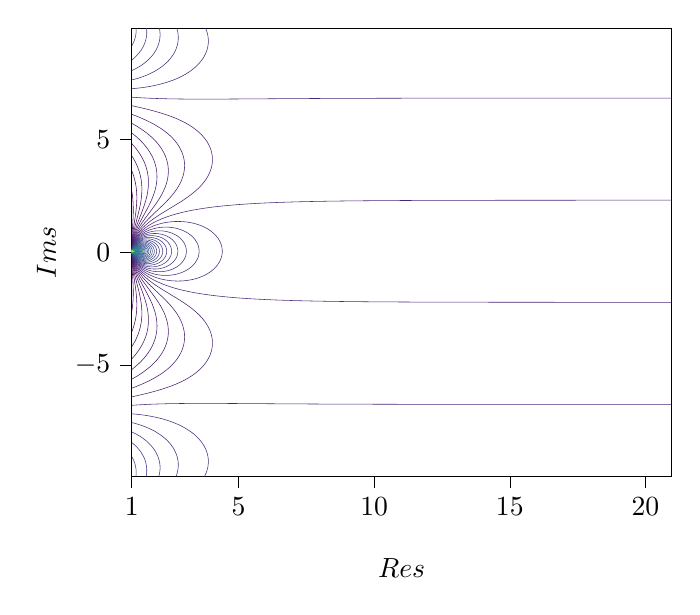
\begin{tikzpicture}

\definecolor{color0}{rgb}{0.269944,0.014625,0.341379}
\definecolor{color1}{rgb}{0.273809,0.031497,0.358853}
\definecolor{color2}{rgb}{0.277018,0.050344,0.375715}
\definecolor{color3}{rgb}{0.279566,0.067836,0.391917}
\definecolor{color4}{rgb}{0.281446,0.08432,0.407414}
\definecolor{color5}{rgb}{0.282656,0.100196,0.42216}
\definecolor{color6}{rgb}{0.283197,0.11568,0.436115}
\definecolor{color7}{rgb}{0.283072,0.130895,0.449241}
\definecolor{color8}{rgb}{0.28229,0.145912,0.46151}
\definecolor{color9}{rgb}{0.280868,0.160771,0.472899}
\definecolor{color10}{rgb}{0.278826,0.17549,0.483397}
\definecolor{color11}{rgb}{0.276194,0.190074,0.493001}
\definecolor{color12}{rgb}{0.273006,0.20452,0.501721}
\definecolor{color13}{rgb}{0.269308,0.218818,0.509577}
\definecolor{color14}{rgb}{0.265145,0.232956,0.516599}
\definecolor{color15}{rgb}{0.260571,0.246922,0.522828}
\definecolor{color16}{rgb}{0.255645,0.260703,0.528312}
\definecolor{color17}{rgb}{0.250425,0.27429,0.533103}
\definecolor{color18}{rgb}{0.244972,0.287675,0.53726}
\definecolor{color19}{rgb}{0.239346,0.300855,0.540844}
\definecolor{color20}{rgb}{0.233603,0.313828,0.543914}
\definecolor{color21}{rgb}{0.227802,0.326594,0.546532}
\definecolor{color22}{rgb}{0.221989,0.339161,0.548752}
\definecolor{color23}{rgb}{0.21621,0.351535,0.550627}
\definecolor{color24}{rgb}{0.210503,0.363727,0.552206}
\definecolor{color25}{rgb}{0.204903,0.375746,0.553533}
\definecolor{color26}{rgb}{0.19943,0.387607,0.554642}
\definecolor{color27}{rgb}{0.1941,0.399323,0.555565}
\definecolor{color28}{rgb}{0.188923,0.41091,0.556326}
\definecolor{color29}{rgb}{0.183898,0.422383,0.556944}
\definecolor{color30}{rgb}{0.179019,0.433756,0.55743}
\definecolor{color31}{rgb}{0.174274,0.445044,0.557792}
\definecolor{color32}{rgb}{0.169646,0.456262,0.55803}
\definecolor{color33}{rgb}{0.165117,0.467423,0.558141}
\definecolor{color34}{rgb}{0.160665,0.47854,0.558115}
\definecolor{color35}{rgb}{0.15627,0.489624,0.557936}
\definecolor{color36}{rgb}{0.151918,0.500685,0.557587}
\definecolor{color37}{rgb}{0.147607,0.511733,0.557049}
\definecolor{color38}{rgb}{0.143343,0.522773,0.556295}
\definecolor{color39}{rgb}{0.139147,0.533812,0.555298}
\definecolor{color40}{rgb}{0.135066,0.544853,0.554029}
\definecolor{color41}{rgb}{0.131172,0.555899,0.552459}
\definecolor{color42}{rgb}{0.127568,0.566949,0.550556}
\definecolor{color43}{rgb}{0.125394,0.574318,0.549086}
\definecolor{color44}{rgb}{0.122606,0.585371,0.546557}
\definecolor{color45}{rgb}{0.120565,0.596422,0.543611}
\definecolor{color46}{rgb}{0.119512,0.607464,0.540218}
\definecolor{color47}{rgb}{0.119699,0.61849,0.536347}
\definecolor{color48}{rgb}{0.12138,0.629492,0.531973}
\definecolor{color49}{rgb}{0.12478,0.640461,0.527068}
\definecolor{color50}{rgb}{0.130067,0.651384,0.521608}
\definecolor{color51}{rgb}{0.137339,0.662252,0.515571}
\definecolor{color52}{rgb}{0.146616,0.67305,0.508936}
\definecolor{color53}{rgb}{0.157851,0.683765,0.501686}
\definecolor{color54}{rgb}{0.170948,0.694384,0.493803}
\definecolor{color55}{rgb}{0.185783,0.704891,0.485273}
\definecolor{color56}{rgb}{0.202219,0.715272,0.476084}
\definecolor{color57}{rgb}{0.220124,0.725509,0.466226}
\definecolor{color58}{rgb}{0.239374,0.735588,0.455688}
\definecolor{color59}{rgb}{0.259857,0.745492,0.444467}
\definecolor{color60}{rgb}{0.281477,0.755203,0.432552}
\definecolor{color61}{rgb}{0.304148,0.764704,0.419943}
\definecolor{color62}{rgb}{0.327796,0.77398,0.40664}
\definecolor{color63}{rgb}{0.35236,0.783011,0.392636}
\definecolor{color64}{rgb}{0.377779,0.791781,0.377939}
\definecolor{color65}{rgb}{0.404001,0.800275,0.362552}
\definecolor{color66}{rgb}{0.430983,0.808473,0.346476}
\definecolor{color67}{rgb}{0.458674,0.816363,0.329727}
\definecolor{color68}{rgb}{0.487026,0.823929,0.312321}
\definecolor{color69}{rgb}{0.515992,0.831158,0.294279}
\definecolor{color70}{rgb}{0.545524,0.838039,0.275626}
\definecolor{color71}{rgb}{0.575563,0.844566,0.256415}
\definecolor{color72}{rgb}{0.606045,0.850733,0.236712}
\definecolor{color73}{rgb}{0.636902,0.856542,0.21662}
\definecolor{color74}{rgb}{0.668054,0.861999,0.196293}
\definecolor{color75}{rgb}{0.699415,0.867117,0.175971}
\definecolor{color76}{rgb}{0.730889,0.871916,0.156029}
\definecolor{color77}{rgb}{0.762373,0.876424,0.137064}
\definecolor{color78}{rgb}{0.79376,0.880678,0.120005}
\definecolor{color79}{rgb}{0.82494,0.88472,0.106217}
\definecolor{color80}{rgb}{0.85581,0.888601,0.097452}
\definecolor{color81}{rgb}{0.886271,0.892374,0.095374}
\definecolor{color82}{rgb}{0.916242,0.896091,0.100717}
\definecolor{color83}{rgb}{0.945636,0.899815,0.112838}
\definecolor{color84}{rgb}{0.974417,0.90359,0.130215}

\begin{axis}[
tick align=outside,
tick pos=left,
x grid style={white!69.0196078431373!black},
xmin=1.06, xmax=20.96,
xtick style={color=black},
y grid style={white!69.0196078431373!black},
ymin=-9.95, ymax=9.95,
ytick style={color=black},
extra x ticks = {1.06},
extra x tick labels = {$1$},
xlabel= $\operatorname{Re} s$,
ylabel = $\operatorname{Im} s$,
]
\path [draw=color0, very thin]
(axis cs:1.06,-0.453088282945391)
--(axis cs:1.0649381809945,-0.549999999999999)
--(axis cs:1.07003399666962,-0.65)
--(axis cs:1.07525977479044,-0.75)
--(axis cs:1.08059975801296,-0.85)
--(axis cs:1.08598327438163,-0.949999999999999)
--(axis cs:1.09130851124041,-1.05)
--(axis cs:1.09645447751238,-1.15)
--(axis cs:1.10128782455856,-1.25)
--(axis cs:1.10566719377048,-1.35)
--(axis cs:1.10944624998754,-1.45)
--(axis cs:1.11247593542732,-1.55)
--(axis cs:1.11460620144988,-1.65)
--(axis cs:1.11568734561554,-1.75)
--(axis cs:1.11557101852994,-1.85)
--(axis cs:1.11411093393389,-1.95)
--(axis cs:1.11116330025994,-2.05)
--(axis cs:1.10658698458941,-2.15)
--(axis cs:1.10024341658333,-2.25)
--(axis cs:1.09199623838039,-2.35)
--(axis cs:1.08171070545474,-2.45)
--(axis cs:1.06925284231282,-2.55)
--(axis cs:1.06,-2.61388235207933);

\path [draw=color0, very thin]
(axis cs:1.06,2.71388235207933)
--(axis cs:1.06925284231282,2.65)
--(axis cs:1.08171070545474,2.55)
--(axis cs:1.09199623838039,2.45)
--(axis cs:1.10024341658333,2.35)
--(axis cs:1.10658698458941,2.25)
--(axis cs:1.11116330025994,2.15)
--(axis cs:1.11411093393389,2.05)
--(axis cs:1.11557101852994,1.95)
--(axis cs:1.11568734561554,1.85)
--(axis cs:1.11460620144988,1.75)
--(axis cs:1.11247593542732,1.65)
--(axis cs:1.10944624998754,1.55)
--(axis cs:1.10566719377048,1.45)
--(axis cs:1.10128782455856,1.35)
--(axis cs:1.09645447751238,1.25)
--(axis cs:1.09130851124041,1.15)
--(axis cs:1.08598327438163,1.05)
--(axis cs:1.08059975801296,0.950000000000001)
--(axis cs:1.07525977479044,0.850000000000001)
--(axis cs:1.07003399666962,0.75)
--(axis cs:1.0649381809945,0.65)
--(axis cs:1.06,0.553088282945393);

\path [draw=color1, very thin]
(axis cs:1.06,-0.31627220025223)
--(axis cs:1.06377452867858,-0.35)
--(axis cs:1.0722375503661,-0.449999999999999)
--(axis cs:1.08100069071506,-0.549999999999999)
--(axis cs:1.09038906364148,-0.65)
--(axis cs:1.10046931562014,-0.75)
--(axis cs:1.111194854058,-0.85)
--(axis cs:1.12246073337773,-0.949999999999999)
--(axis cs:1.13412823825703,-1.05)
--(axis cs:1.14603762938363,-1.15)
--(axis cs:1.15801569426702,-1.25)
--(axis cs:1.16,-1.26852201825282)
--(axis cs:1.1711340531582,-1.35)
--(axis cs:1.18385630384569,-1.45)
--(axis cs:1.19579499097366,-1.55)
--(axis cs:1.20682556664918,-1.65)
--(axis cs:1.21680855091049,-1.75)
--(axis cs:1.22559591538958,-1.85)
--(axis cs:1.23303544765562,-1.95)
--(axis cs:1.23897372708724,-2.05)
--(axis cs:1.24325809542154,-2.15)
--(axis cs:1.2457378627504,-2.25)
--(axis cs:1.24626490540192,-2.35)
--(axis cs:1.24469376060101,-2.45)
--(axis cs:1.24088129009074,-2.55)
--(axis cs:1.23468596306295,-2.65)
--(axis cs:1.22596679313132,-2.75)
--(axis cs:1.21458195187156,-2.85)
--(axis cs:1.20038707089336,-2.95)
--(axis cs:1.1832332343422,-3.05)
--(axis cs:1.16296465333092,-3.15)
--(axis cs:1.16,-3.16303158845932)
--(axis cs:1.14026316351631,-3.25)
--(axis cs:1.11435182284167,-3.35)
--(axis cs:1.08492688145678,-3.45)
--(axis cs:1.06,-3.52590397343815);

\path [draw=color1, very thin]
(axis cs:1.06,3.62590397343815)
--(axis cs:1.08492688145678,3.55)
--(axis cs:1.11435182284167,3.45)
--(axis cs:1.14026316351631,3.35)
--(axis cs:1.16,3.26303158845932)
--(axis cs:1.16296465333092,3.25)
--(axis cs:1.1832332343422,3.15)
--(axis cs:1.20038707089336,3.05)
--(axis cs:1.21458195187156,2.95)
--(axis cs:1.22596679313132,2.85)
--(axis cs:1.23468596306295,2.75)
--(axis cs:1.24088129009074,2.65)
--(axis cs:1.24469376060101,2.55)
--(axis cs:1.24626490540192,2.45)
--(axis cs:1.2457378627504,2.35)
--(axis cs:1.24325809542154,2.25)
--(axis cs:1.23897372708724,2.15)
--(axis cs:1.23303544765562,2.05)
--(axis cs:1.22559591538958,1.95)
--(axis cs:1.21680855091049,1.85)
--(axis cs:1.20682556664918,1.75)
--(axis cs:1.19579499097366,1.65)
--(axis cs:1.18385630384569,1.55)
--(axis cs:1.1711340531582,1.45)
--(axis cs:1.16,1.36852201825283)
--(axis cs:1.15801569426702,1.35)
--(axis cs:1.14603762938363,1.25)
--(axis cs:1.13412823825703,1.15)
--(axis cs:1.12246073337773,1.05)
--(axis cs:1.111194854058,0.950000000000001)
--(axis cs:1.10046931562014,0.850000000000001)
--(axis cs:1.09038906364148,0.75)
--(axis cs:1.08100069071506,0.65)
--(axis cs:1.0722375503661,0.550000000000001)
--(axis cs:1.06377452867858,0.450000000000001)
--(axis cs:1.06,0.416272200252231);

\path [draw=color2, very thin]
(axis cs:1.06,-0.243441689803711)
--(axis cs:1.06136030142452,-0.25)
--(axis cs:1.07304120125452,-0.35)
--(axis cs:1.08459617857151,-0.449999999999999)
--(axis cs:1.09706320043562,-0.549999999999999)
--(axis cs:1.11074413061334,-0.65)
--(axis cs:1.12567885644983,-0.75)
--(axis cs:1.14178995010305,-0.85)
--(axis cs:1.15893819237382,-0.949999999999999)
--(axis cs:1.16,-0.956850585934016)
--(axis cs:1.18027470303434,-1.05)
--(axis cs:1.20158321510241,-1.15)
--(axis cs:1.22267018139569,-1.25)
--(axis cs:1.24349249784387,-1.35)
--(axis cs:1.26,-1.43223570832515)
--(axis cs:1.26445227465427,-1.45)
--(axis cs:1.28662617276495,-1.55)
--(axis cs:1.30761745194117,-1.65)
--(axis cs:1.32736237939509,-1.75)
--(axis cs:1.34576225605761,-1.85)
--(axis cs:1.36,-1.93496780033748)
--(axis cs:1.36293153916638,-1.95)
--(axis cs:1.37948418238324,-2.05)
--(axis cs:1.39399469104993,-2.15)
--(axis cs:1.40637043137459,-2.25)
--(axis cs:1.4165061778706,-2.35)
--(axis cs:1.4242883712944,-2.45)
--(axis cs:1.42959781400185,-2.55)
--(axis cs:1.43231119052244,-2.65)
--(axis cs:1.4323016748144,-2.75)
--(axis cs:1.42943880211074,-2.85)
--(axis cs:1.42358772575939,-2.95)
--(axis cs:1.41460793788902,-3.05)
--(axis cs:1.40235150079454,-3.15)
--(axis cs:1.38666080953941,-3.25)
--(axis cs:1.36736588260579,-3.35)
--(axis cs:1.36,-3.38270482698374)
--(axis cs:1.34496540789294,-3.45)
--(axis cs:1.31904476672278,-3.55)
--(axis cs:1.28906423339381,-3.65)
--(axis cs:1.26,-3.73523488081659)
--(axis cs:1.25499912269147,-3.75)
--(axis cs:1.2177542079331,-3.85)
--(axis cs:1.17583308332237,-3.95)
--(axis cs:1.16,-3.98453352799529)
--(axis cs:1.13018116343902,-4.05)
--(axis cs:1.08003599065735,-4.15)
--(axis cs:1.06,-4.18679732024643);

\path [draw=color2, very thin]
(axis cs:1.06,4.28679732024643)
--(axis cs:1.08003599065735,4.25)
--(axis cs:1.13018116343902,4.15)
--(axis cs:1.16,4.0845335279953)
--(axis cs:1.17583308332237,4.05)
--(axis cs:1.2177542079331,3.95)
--(axis cs:1.25499912269147,3.85)
--(axis cs:1.26,3.83523488081659)
--(axis cs:1.28906423339381,3.75)
--(axis cs:1.31904476672278,3.65)
--(axis cs:1.34496540789294,3.55)
--(axis cs:1.36,3.48270482698374)
--(axis cs:1.36736588260579,3.45)
--(axis cs:1.38666080953941,3.35)
--(axis cs:1.40235150079454,3.25)
--(axis cs:1.41460793788902,3.15)
--(axis cs:1.42358772575939,3.05)
--(axis cs:1.42943880211074,2.95)
--(axis cs:1.4323016748144,2.85)
--(axis cs:1.43231119052244,2.75)
--(axis cs:1.42959781400185,2.65)
--(axis cs:1.4242883712944,2.55)
--(axis cs:1.4165061778706,2.45)
--(axis cs:1.40637043137459,2.35)
--(axis cs:1.39399469104993,2.25)
--(axis cs:1.37948418238324,2.15)
--(axis cs:1.36293153916638,2.05)
--(axis cs:1.36,2.03496780033748)
--(axis cs:1.34576225605761,1.95)
--(axis cs:1.32736237939509,1.85)
--(axis cs:1.30761745194117,1.75)
--(axis cs:1.28662617276495,1.65)
--(axis cs:1.26445227465427,1.55)
--(axis cs:1.26,1.53223570832515)
--(axis cs:1.24349249784387,1.45)
--(axis cs:1.22267018139569,1.35)
--(axis cs:1.20158321510241,1.25)
--(axis cs:1.18027470303434,1.15)
--(axis cs:1.16,1.05685058593402)
--(axis cs:1.15893819237382,1.05)
--(axis cs:1.14178995010305,0.950000000000001)
--(axis cs:1.12567885644983,0.850000000000001)
--(axis cs:1.11074413061334,0.75)
--(axis cs:1.09706320043562,0.65)
--(axis cs:1.08459617857151,0.550000000000001)
--(axis cs:1.07304120125452,0.450000000000001)
--(axis cs:1.06136030142452,0.350000000000001)
--(axis cs:1.06,0.343441689803713);

\path [draw=color3, very thin]
(axis cs:1.06,-0.210591943204179)
--(axis cs:1.06817387927566,-0.25)
--(axis cs:1.08230787383045,-0.35)
--(axis cs:1.09695480677692,-0.449999999999999)
--(axis cs:1.11312571015617,-0.549999999999999)
--(axis cs:1.13109919758521,-0.65)
--(axis cs:1.15088839727953,-0.75)
--(axis cs:1.16,-0.797169929211184)
--(axis cs:1.17590894729866,-0.85)
--(axis cs:1.20370395654235,-0.949999999999999)
--(axis cs:1.23149956898463,-1.05)
--(axis cs:1.25946591158131,-1.15)
--(axis cs:1.26,-1.15212406130015)
--(axis cs:1.29216948656554,-1.25)
--(axis cs:1.32392880129676,-1.35)
--(axis cs:1.3547969060484,-1.45)
--(axis cs:1.36,-1.46856506763678)
--(axis cs:1.38796893391712,-1.55)
--(axis cs:1.42007924190086,-1.65)
--(axis cs:1.45048786404417,-1.75)
--(axis cs:1.46,-1.78453399522731)
--(axis cs:1.48120780983025,-1.85)
--(axis cs:1.51061118503943,-1.95)
--(axis cs:1.53767816963652,-2.05)
--(axis cs:1.56,-2.14067065778393)
--(axis cs:1.56262671538701,-2.15)
--(axis cs:1.58680782406697,-2.25)
--(axis cs:1.60814659727948,-2.35)
--(axis cs:1.62663837244377,-2.45)
--(axis cs:1.64224898237645,-2.55)
--(axis cs:1.65492245414917,-2.65)
--(axis cs:1.66,-2.70350963044071)
--(axis cs:1.66488164565157,-2.75)
--(axis cs:1.67184026970091,-2.85)
--(axis cs:1.67538521118062,-2.95)
--(axis cs:1.67542877492402,-3.05)
--(axis cs:1.67186564635642,-3.15)
--(axis cs:1.66457279759079,-3.25)
--(axis cs:1.66,-3.29177402550373)
--(axis cs:1.65373335299705,-3.35)
--(axis cs:1.63926034144125,-3.45)
--(axis cs:1.62073980820762,-3.55)
--(axis cs:1.59796559355316,-3.65)
--(axis cs:1.57070345415338,-3.75)
--(axis cs:1.56,-3.78420303280828)
--(axis cs:1.53962968695168,-3.85)
--(axis cs:1.50417351166796,-3.95)
--(axis cs:1.46352231432198,-4.05)
--(axis cs:1.46,-4.05787562652246)
--(axis cs:1.41912665075558,-4.15)
--(axis cs:1.36911432068158,-4.25)
--(axis cs:1.36,-4.2667085070508)
--(axis cs:1.31486028631409,-4.35)
--(axis cs:1.26,-4.44116491339772)
--(axis cs:1.25471504341086,-4.45)
--(axis cs:1.19010669296949,-4.55)
--(axis cs:1.16,-4.59271545096931)
--(axis cs:1.11983608051045,-4.65)
--(axis cs:1.06,-4.72854008548203);

\path [draw=color3, very thin]
(axis cs:1.06,4.82854008548203)
--(axis cs:1.11983608051045,4.75)
--(axis cs:1.16,4.69271545096931)
--(axis cs:1.19010669296949,4.65)
--(axis cs:1.25471504341086,4.55)
--(axis cs:1.26,4.54116491339772)
--(axis cs:1.31486028631409,4.45)
--(axis cs:1.36,4.3667085070508)
--(axis cs:1.36911432068158,4.35)
--(axis cs:1.41912665075558,4.25)
--(axis cs:1.46,4.15787562652246)
--(axis cs:1.46352231432198,4.15)
--(axis cs:1.50417351166796,4.05)
--(axis cs:1.53962968695168,3.95)
--(axis cs:1.56,3.88420303280829)
--(axis cs:1.57070345415338,3.85)
--(axis cs:1.59796559355316,3.75)
--(axis cs:1.62073980820762,3.65)
--(axis cs:1.63926034144125,3.55)
--(axis cs:1.65373335299705,3.45)
--(axis cs:1.66,3.39177402550373)
--(axis cs:1.66457279759079,3.35)
--(axis cs:1.67186564635642,3.25)
--(axis cs:1.67542877492402,3.15)
--(axis cs:1.67538521118062,3.05)
--(axis cs:1.67184026970091,2.95)
--(axis cs:1.66488164565157,2.85)
--(axis cs:1.66,2.80350963044071)
--(axis cs:1.65492245414917,2.75)
--(axis cs:1.64224898237645,2.65)
--(axis cs:1.62663837244377,2.55)
--(axis cs:1.60814659727948,2.45)
--(axis cs:1.58680782406697,2.35)
--(axis cs:1.56262671538701,2.25)
--(axis cs:1.56,2.24067065778393)
--(axis cs:1.53767816963652,2.15)
--(axis cs:1.51061118503943,2.05)
--(axis cs:1.48120780983025,1.95)
--(axis cs:1.46,1.88453399522731)
--(axis cs:1.45048786404417,1.85)
--(axis cs:1.42007924190086,1.75)
--(axis cs:1.38796893391712,1.65)
--(axis cs:1.36,1.56856506763678)
--(axis cs:1.3547969060484,1.55)
--(axis cs:1.32392880129676,1.45)
--(axis cs:1.29216948656554,1.35)
--(axis cs:1.26,1.25212406130015)
--(axis cs:1.25946591158131,1.25)
--(axis cs:1.23149956898463,1.15)
--(axis cs:1.20370395654235,1.05)
--(axis cs:1.17590894729866,0.950000000000001)
--(axis cs:1.16,0.897169929211185)
--(axis cs:1.15088839727953,0.850000000000001)
--(axis cs:1.13109919758521,0.75)
--(axis cs:1.11312571015617,0.65)
--(axis cs:1.09695480677692,0.550000000000001)
--(axis cs:1.08230787383045,0.450000000000001)
--(axis cs:1.06817387927566,0.350000000000001)
--(axis cs:1.06,0.31059194320418);

\path [draw=color4, very thin]
(axis cs:1.06,-0.177742196604646)
--(axis cs:1.0749874571268,-0.25)
--(axis cs:1.09157454640639,-0.35)
--(axis cs:1.10931343498232,-0.449999999999999)
--(axis cs:1.12918821987673,-0.549999999999999)
--(axis cs:1.15145426455707,-0.65)
--(axis cs:1.16,-0.689666843217292)
--(axis cs:1.18179992488243,-0.75)
--(axis cs:1.21520922642218,-0.85)
--(axis cs:1.24871821495847,-0.949999999999999)
--(axis cs:1.26,-0.986100484139408)
--(axis cs:1.28778589983751,-1.05)
--(axis cs:1.32827395677767,-1.15)
--(axis cs:1.36,-1.23164685970014)
--(axis cs:1.36927806749205,-1.25)
--(axis cs:1.41432221194918,-1.35)
--(axis cs:1.45733114124501,-1.45)
--(axis cs:1.46,-1.45688665397646)
--(axis cs:1.50411687684134,-1.55)
--(axis cs:1.54846595017775,-1.65)
--(axis cs:1.56,-1.67864228707082)
--(axis cs:1.5941086076485,-1.75)
--(axis cs:1.63787660682233,-1.85)
--(axis cs:1.66,-1.90545180199685)
--(axis cs:1.68062360898238,-1.95)
--(axis cs:1.72215846433731,-2.05)
--(axis cs:1.76,-2.14954161076408)
--(axis cs:1.76019866984125,-2.15)
--(axis cs:1.79812040539942,-2.25)
--(axis cs:1.83219652344828,-2.35)
--(axis cs:1.86,-2.44157968875888)
--(axis cs:1.8628608510811,-2.45)
--(axis cs:1.89191638346497,-2.55)
--(axis cs:1.91705498498093,-2.65)
--(axis cs:1.93839343521059,-2.75)
--(axis cs:1.95599564205015,-2.85)
--(axis cs:1.96,-2.87944014335388)
--(axis cs:1.9705435884278,-2.95)
--(axis cs:1.98132853836184,-3.05)
--(axis cs:1.98806920388757,-3.15)
--(axis cs:1.99072833953227,-3.25)
--(axis cs:1.98923586591493,-3.35)
--(axis cs:1.98349016292981,-3.45)
--(axis cs:1.97335783433547,-3.55)
--(axis cs:1.96,-3.64120424587749)
--(axis cs:1.95873900222156,-3.65)
--(axis cs:1.94025612898823,-3.75)
--(axis cs:1.91698388652344,-3.85)
--(axis cs:1.88864320769527,-3.95)
--(axis cs:1.86,-4.03533221134945)
--(axis cs:1.85514224171942,-4.05)
--(axis cs:1.81743814548265,-4.15)
--(axis cs:1.77375822655652,-4.25)
--(axis cs:1.76,-4.27817740517957)
--(axis cs:1.72522918637682,-4.35)
--(axis cs:1.67054745367053,-4.45)
--(axis cs:1.66,-4.46754919920523)
--(axis cs:1.61071619985508,-4.55)
--(axis cs:1.56,-4.6262065941301)
--(axis cs:1.5442293058722,-4.65)
--(axis cs:1.47165369199067,-4.75)
--(axis cs:1.46,-4.76477738237623)
--(axis cs:1.39289788269257,-4.85)
--(axis cs:1.36,-4.88835952664065)
--(axis cs:1.30717191715632,-4.95)
--(axis cs:1.26,-5.00083066615165)
--(axis cs:1.21437008501033,-5.05)
--(axis cs:1.16,-5.10437044857356)
--(axis cs:1.11434890281016,-5.15)
--(axis cs:1.06,-5.20061795664761);

\path [draw=color4, very thin]
(axis cs:1.06,5.30061795664761)
--(axis cs:1.11434890281016,5.25)
--(axis cs:1.16,5.20437044857357)
--(axis cs:1.21437008501033,5.15)
--(axis cs:1.26,5.10083066615165)
--(axis cs:1.30717191715632,5.05)
--(axis cs:1.36,4.98835952664065)
--(axis cs:1.39289788269257,4.95)
--(axis cs:1.46,4.86477738237623)
--(axis cs:1.47165369199067,4.85)
--(axis cs:1.5442293058722,4.75)
--(axis cs:1.56,4.7262065941301)
--(axis cs:1.61071619985508,4.65)
--(axis cs:1.66,4.56754919920523)
--(axis cs:1.67054745367053,4.55)
--(axis cs:1.72522918637682,4.45)
--(axis cs:1.76,4.37817740517957)
--(axis cs:1.77375822655652,4.35)
--(axis cs:1.81743814548265,4.25)
--(axis cs:1.85514224171942,4.15)
--(axis cs:1.86,4.13533221134945)
--(axis cs:1.88864320769527,4.05)
--(axis cs:1.91698388652344,3.95)
--(axis cs:1.94025612898823,3.85)
--(axis cs:1.95873900222156,3.75)
--(axis cs:1.96,3.74120424587749)
--(axis cs:1.97335783433547,3.65)
--(axis cs:1.98349016292981,3.55)
--(axis cs:1.98923586591493,3.45)
--(axis cs:1.99072833953227,3.35)
--(axis cs:1.98806920388757,3.25)
--(axis cs:1.98132853836184,3.15)
--(axis cs:1.9705435884278,3.05)
--(axis cs:1.96,2.97944014335388)
--(axis cs:1.95599564205015,2.95)
--(axis cs:1.93839343521059,2.85)
--(axis cs:1.91705498498093,2.75)
--(axis cs:1.89191638346497,2.65)
--(axis cs:1.8628608510811,2.55)
--(axis cs:1.86,2.54157968875888)
--(axis cs:1.83219652344828,2.45)
--(axis cs:1.79812040539942,2.35)
--(axis cs:1.76019866984125,2.25)
--(axis cs:1.76,2.24954161076408)
--(axis cs:1.72215846433731,2.15)
--(axis cs:1.68062360898238,2.05)
--(axis cs:1.66,2.00545180199685)
--(axis cs:1.63787660682233,1.95)
--(axis cs:1.5941086076485,1.85)
--(axis cs:1.56,1.77864228707082)
--(axis cs:1.54846595017775,1.75)
--(axis cs:1.50411687684134,1.65)
--(axis cs:1.46,1.55688665397646)
--(axis cs:1.45733114124501,1.55)
--(axis cs:1.41432221194918,1.45)
--(axis cs:1.36927806749205,1.35)
--(axis cs:1.36,1.33164685970014)
--(axis cs:1.32827395677767,1.25)
--(axis cs:1.28778589983751,1.15)
--(axis cs:1.26,1.08610048413941)
--(axis cs:1.24871821495847,1.05)
--(axis cs:1.21520922642218,0.950000000000001)
--(axis cs:1.18179992488243,0.850000000000001)
--(axis cs:1.16,0.789666843217292)
--(axis cs:1.15145426455707,0.75)
--(axis cs:1.12918821987673,0.65)
--(axis cs:1.10931343498232,0.550000000000001)
--(axis cs:1.09157454640639,0.450000000000001)
--(axis cs:1.0749874571268,0.350000000000001)
--(axis cs:1.06,0.277742196604647);

\path [draw=color5, very thin]
(axis cs:1.06,-0.148540502500346)
--(axis cs:1.06078968144882,-0.149999999999999)
--(axis cs:1.08180103497794,-0.25)
--(axis cs:1.10084121898232,-0.35)
--(axis cs:1.12167206318773,-0.449999999999999)
--(axis cs:1.14525072959729,-0.549999999999999)
--(axis cs:1.16,-0.61128114442762)
--(axis cs:1.17717305739303,-0.65)
--(axis cs:1.21593883712568,-0.75)
--(axis cs:1.25450950554571,-0.85)
--(axis cs:1.26,-0.865713586186267)
--(axis cs:1.30264880002098,-0.949999999999999)
--(axis cs:1.35042019629244,-1.05)
--(axis cs:1.36,-1.07208483513501)
--(axis cs:1.4051226830035,-1.15)
--(axis cs:1.45892835010764,-1.25)
--(axis cs:1.46,-1.25222477321311)
--(axis cs:1.51958479741923,-1.35)
--(axis cs:1.56,-1.42211256510872)
--(axis cs:1.57930341183264,-1.45)
--(axis cs:1.64112398140451,-1.55)
--(axis cs:1.66,-1.58378040228193)
--(axis cs:1.7042285822809,-1.65)
--(axis cs:1.76,-1.74239749640232)
--(axis cs:1.76539748850236,-1.75)
--(axis cs:1.82839171793739,-1.85)
--(axis cs:1.86,-1.90565769304205)
--(axis cs:1.8889954632921,-1.95)
--(axis cs:1.94743202341986,-2.05)
--(axis cs:1.96,-2.0740863428938)
--(axis cs:2.00486562409382,-2.15)
--(axis cs:2.05775346110963,-2.25)
--(axis cs:2.06,-2.25480051657502)
--(axis cs:2.10982474193466,-2.35)
--(axis cs:2.15642531765538,-2.45)
--(axis cs:2.16,-2.45875100846584)
--(axis cs:2.20128143453837,-2.55)
--(axis cs:2.24101004747819,-2.65)
--(axis cs:2.26,-2.70508398581458)
--(axis cs:2.27702300691527,-2.75)
--(axis cs:2.30935734302974,-2.85)
--(axis cs:2.33674180749449,-2.95)
--(axis cs:2.35942633835285,-3.05)
--(axis cs:2.36,-3.05322183371127)
--(axis cs:2.3787914702634,-3.15)
--(axis cs:2.39337714131548,-3.25)
--(axis cs:2.40323707432816,-3.35)
--(axis cs:2.40840527215252,-3.45)
--(axis cs:2.40886132963277,-3.55)
--(axis cs:2.40453406539005,-3.65)
--(axis cs:2.39530269528631,-3.75)
--(axis cs:2.38099582454548,-3.85)
--(axis cs:2.36138836346281,-3.95)
--(axis cs:2.36,-3.95567053457078)
--(axis cs:2.33740961608842,-4.05)
--(axis cs:2.30782780131832,-4.15)
--(axis cs:2.27216189551309,-4.25)
--(axis cs:2.26,-4.27952562869318)
--(axis cs:2.23137211404543,-4.35)
--(axis cs:2.18431532350246,-4.45)
--(axis cs:2.16,-4.49551742407826)
--(axis cs:2.13114585791549,-4.55)
--(axis cs:2.07114571582618,-4.65)
--(axis cs:2.06,-4.66677577631708)
--(axis cs:2.00491062670959,-4.75)
--(axis cs:1.96,-4.81075049165436)
--(axis cs:1.93101742719685,-4.85)
--(axis cs:1.86,-4.93696962564475)
--(axis cs:1.84934697370323,-4.95)
--(axis cs:1.76,-5.04963366637549)
--(axis cs:1.75967038932582,-5.05)
--(axis cs:1.66173624812598,-5.15)
--(axis cs:1.66,-5.15163357176669)
--(axis cs:1.56,-5.24522547379311)
--(axis cs:1.55486643351652,-5.25)
--(axis cs:1.46,-5.33184411730437)
--(axis cs:1.4387669837877,-5.35)
--(axis cs:1.36,-5.41273248139032)
--(axis cs:1.31270943451152,-5.45)
--(axis cs:1.26,-5.48882422988635)
--(axis cs:1.17592608534493,-5.55)
--(axis cs:1.16,-5.56086379392219)
--(axis cs:1.06,-5.62912612401772);

\path [draw=color5, very thin]
(axis cs:1.06,5.72912612401772)
--(axis cs:1.16,5.66086379392219)
--(axis cs:1.17592608534493,5.65)
--(axis cs:1.26,5.58882422988635)
--(axis cs:1.31270943451152,5.55)
--(axis cs:1.36,5.51273248139032)
--(axis cs:1.4387669837877,5.45)
--(axis cs:1.46,5.43184411730437)
--(axis cs:1.55486643351652,5.35)
--(axis cs:1.56,5.34522547379311)
--(axis cs:1.66,5.25163357176669)
--(axis cs:1.66173624812598,5.25)
--(axis cs:1.75967038932582,5.15)
--(axis cs:1.76,5.14963366637549)
--(axis cs:1.84934697370323,5.05)
--(axis cs:1.86,5.03696962564475)
--(axis cs:1.93101742719685,4.95)
--(axis cs:1.96,4.91075049165436)
--(axis cs:2.00491062670959,4.85)
--(axis cs:2.06,4.76677577631708)
--(axis cs:2.07114571582618,4.75)
--(axis cs:2.13114585791549,4.65)
--(axis cs:2.16,4.59551742407826)
--(axis cs:2.18431532350246,4.55)
--(axis cs:2.23137211404543,4.45)
--(axis cs:2.26,4.37952562869318)
--(axis cs:2.27216189551309,4.35)
--(axis cs:2.30782780131832,4.25)
--(axis cs:2.33740961608842,4.15)
--(axis cs:2.36,4.05567053457078)
--(axis cs:2.36138836346281,4.05)
--(axis cs:2.38099582454548,3.95)
--(axis cs:2.39530269528631,3.85)
--(axis cs:2.40453406539005,3.75)
--(axis cs:2.40886132963277,3.65)
--(axis cs:2.40840527215252,3.55)
--(axis cs:2.40323707432816,3.45)
--(axis cs:2.39337714131548,3.35)
--(axis cs:2.3787914702634,3.25)
--(axis cs:2.36,3.15322183371127)
--(axis cs:2.35942633835285,3.15)
--(axis cs:2.33674180749449,3.05)
--(axis cs:2.30935734302974,2.95)
--(axis cs:2.27702300691527,2.85)
--(axis cs:2.26,2.80508398581458)
--(axis cs:2.24101004747819,2.75)
--(axis cs:2.20128143453837,2.65)
--(axis cs:2.16,2.55875100846584)
--(axis cs:2.15642531765538,2.55)
--(axis cs:2.10982474193466,2.45)
--(axis cs:2.06,2.35480051657502)
--(axis cs:2.05775346110964,2.35)
--(axis cs:2.00486562409382,2.25)
--(axis cs:1.96,2.1740863428938)
--(axis cs:1.94743202341986,2.15)
--(axis cs:1.8889954632921,2.05)
--(axis cs:1.86,2.00565769304205)
--(axis cs:1.82839171793739,1.95)
--(axis cs:1.76539748850236,1.85)
--(axis cs:1.76,1.84239749640232)
--(axis cs:1.7042285822809,1.75)
--(axis cs:1.66,1.68378040228193)
--(axis cs:1.64112398140451,1.65)
--(axis cs:1.57930341183264,1.55)
--(axis cs:1.56,1.52211256510872)
--(axis cs:1.51958479741923,1.45)
--(axis cs:1.46,1.35222477321311)
--(axis cs:1.45892835010764,1.35)
--(axis cs:1.4051226830035,1.25)
--(axis cs:1.36,1.17208483513501)
--(axis cs:1.35042019629244,1.15)
--(axis cs:1.30264880002098,1.05)
--(axis cs:1.26,0.965713586186269)
--(axis cs:1.25450950554571,0.950000000000001)
--(axis cs:1.21593883712568,0.850000000000001)
--(axis cs:1.17717305739303,0.75)
--(axis cs:1.16,0.71128114442762)
--(axis cs:1.14525072959729,0.65)
--(axis cs:1.12167206318773,0.550000000000001)
--(axis cs:1.10084121898232,0.450000000000001)
--(axis cs:1.08180103497794,0.350000000000001)
--(axis cs:1.06078968144882,0.25)
--(axis cs:1.06,0.248540502500347);

\path [draw=color6, very thin]
(axis cs:1.06,-0.139153590365513)
--(axis cs:1.06586860099228,-0.149999999999999)
--(axis cs:1.08861461282908,-0.25)
--(axis cs:1.11010789155826,-0.35)
--(axis cs:1.13403069139314,-0.449999999999999)
--(axis cs:1.16,-0.546254901810962)
--(axis cs:1.16210832069065,-0.549999999999999)
--(axis cs:1.20677327079124,-0.65)
--(axis cs:1.25007774936893,-0.75)
--(axis cs:1.26,-0.775252762334925)
--(axis cs:1.30460611777963,-0.85)
--(axis cs:1.35956143977801,-0.949999999999999)
--(axis cs:1.36,-0.950901524469071)
--(axis cs:1.42630409559123,-1.05)
--(axis cs:1.46,-1.10560078856795)
--(axis cs:1.4955408483743,-1.15)
--(axis cs:1.56,-1.24097888548205)
--(axis cs:1.56816488134008,-1.25)
--(axis cs:1.64722050466093,-1.35)
--(axis cs:1.66,-1.36819799510289)
--(axis cs:1.73036513849936,-1.45)
--(axis cs:1.76,-1.48893391281809)
--(axis cs:1.81574529134309,-1.55)
--(axis cs:1.86,-1.60494991972402)
--(axis cs:1.90272146254988,-1.65)
--(axis cs:1.96,-1.71854749509104)
--(axis cs:1.99045681360042,-1.75)
--(axis cs:2.06,-1.83153738540901)
--(axis cs:2.07799774328623,-1.85)
--(axis cs:2.16,-1.94551838873066)
--(axis cs:2.16434535069407,-1.95)
--(axis cs:2.24983757424714,-2.05)
--(axis cs:2.26,-2.06345714792948)
--(axis cs:2.33289565519561,-2.15)
--(axis cs:2.36,-2.18650099933824)
--(axis cs:2.41218003300003,-2.25)
--(axis cs:2.46,-2.31611857203182)
--(axis cs:2.48693661208512,-2.35)
--(axis cs:2.55679868307712,-2.45)
--(axis cs:2.56,-2.45520406799786)
--(axis cs:2.62370898074438,-2.55)
--(axis cs:2.66,-2.61176802391909)
--(axis cs:2.68443632416457,-2.65)
--(axis cs:2.74018159619115,-2.75)
--(axis cs:2.76,-2.79093577993097)
--(axis cs:2.7910017902072,-2.85)
--(axis cs:2.83620861235768,-2.95)
--(axis cs:2.86,-3.01161478454896)
--(axis cs:2.87603332676663,-3.05)
--(axis cs:2.91117878393262,-3.15)
--(axis cs:2.94025416360271,-3.25)
--(axis cs:2.96,-3.33442174052055)
--(axis cs:2.96393854339569,-3.35)
--(axis cs:2.98323930876832,-3.45)
--(axis cs:2.99694736097661,-3.55)
--(axis cs:3.00521481739622,-3.65)
--(axis cs:3.00810574341849,-3.75)
--(axis cs:3.0056043298352,-3.85)
--(axis cs:2.99761890654076,-3.95)
--(axis cs:2.98398234245254,-4.05)
--(axis cs:2.96444905962208,-4.15)
--(axis cs:2.96,-4.1676781826359)
--(axis cs:2.93984240996381,-4.25)
--(axis cs:2.90914183453555,-4.35)
--(axis cs:2.87158883926217,-4.45)
--(axis cs:2.86,-4.476427805093)
--(axis cs:2.82826841401124,-4.55)
--(axis cs:2.77765694225507,-4.65)
--(axis cs:2.76,-4.68060105172726)
--(axis cs:2.72032381757621,-4.75)
--(axis cs:2.66,-4.84185184687447)
--(axis cs:2.65467602451562,-4.85)
--(axis cs:2.58170621690788,-4.95)
--(axis cs:2.56,-4.97658799785809)
--(axis cs:2.49993187603427,-5.05)
--(axis cs:2.46,-5.09389959666965)
--(axis cs:2.40864780709025,-5.15)
--(axis cs:2.36,-5.19821069809473)
--(axis cs:2.30719800651293,-5.25)
--(axis cs:2.26,-5.29229531738517)
--(axis cs:2.19467018078293,-5.35)
--(axis cs:2.16,-5.37815123913752)
--(axis cs:2.06984875814141,-5.45)
--(axis cs:2.06,-5.45725388839447)
--(axis cs:1.96,-5.5303013545465)
--(axis cs:1.93256974052018,-5.55)
--(axis cs:1.86,-5.59844891075026)
--(axis cs:1.7807181856814,-5.65)
--(axis cs:1.76,-5.66257204442546)
--(axis cs:1.66,-5.72279165197646)
--(axis cs:1.61394834901785,-5.75)
--(axis cs:1.56,-5.77987480360628)
--(axis cs:1.46,-5.83420053756632)
--(axis cs:1.43075223790945,-5.85)
--(axis cs:1.36,-5.88595150464498)
--(axis cs:1.26,-5.93567702095695)
--(axis cs:1.23119888079243,-5.95)
--(axis cs:1.16,-5.98340404068836)
--(axis cs:1.06,-6.02958715526829);

\path [draw=color6, very thin]
(axis cs:1.06,6.12958715526829)
--(axis cs:1.16,6.08340404068836)
--(axis cs:1.23119888079243,6.05)
--(axis cs:1.26,6.03567702095695)
--(axis cs:1.36,5.98595150464498)
--(axis cs:1.43075223790945,5.95)
--(axis cs:1.46,5.93420053756632)
--(axis cs:1.56,5.87987480360628)
--(axis cs:1.61394834901785,5.85)
--(axis cs:1.66,5.82279165197646)
--(axis cs:1.76,5.76257204442546)
--(axis cs:1.7807181856814,5.75)
--(axis cs:1.86,5.69844891075026)
--(axis cs:1.93256974052018,5.65)
--(axis cs:1.96,5.63030135454651)
--(axis cs:2.06,5.55725388839447)
--(axis cs:2.06984875814141,5.55)
--(axis cs:2.16,5.47815123913753)
--(axis cs:2.19467018078293,5.45)
--(axis cs:2.26,5.39229531738517)
--(axis cs:2.30719800651293,5.35)
--(axis cs:2.36,5.29821069809473)
--(axis cs:2.40864780709025,5.25)
--(axis cs:2.46,5.19389959666965)
--(axis cs:2.49993187603427,5.15)
--(axis cs:2.56,5.0765879978581)
--(axis cs:2.58170621690788,5.05)
--(axis cs:2.65467602451562,4.95)
--(axis cs:2.66,4.94185184687447)
--(axis cs:2.72032381757621,4.85)
--(axis cs:2.76,4.78060105172726)
--(axis cs:2.77765694225507,4.75)
--(axis cs:2.82826841401124,4.65)
--(axis cs:2.86,4.576427805093)
--(axis cs:2.87158883926217,4.55)
--(axis cs:2.90914183453555,4.45)
--(axis cs:2.93984240996381,4.35)
--(axis cs:2.96,4.2676781826359)
--(axis cs:2.96444905962208,4.25)
--(axis cs:2.98398234245254,4.15)
--(axis cs:2.99761890654076,4.05)
--(axis cs:3.0056043298352,3.95)
--(axis cs:3.00810574341849,3.85)
--(axis cs:3.00521481739622,3.75)
--(axis cs:2.99694736097661,3.65)
--(axis cs:2.98323930876832,3.55)
--(axis cs:2.96393854339569,3.45)
--(axis cs:2.96,3.43442174052055)
--(axis cs:2.94025416360271,3.35)
--(axis cs:2.91117878393262,3.25)
--(axis cs:2.87603332676663,3.15)
--(axis cs:2.86,3.11161478454896)
--(axis cs:2.83620861235768,3.05)
--(axis cs:2.7910017902072,2.95)
--(axis cs:2.76,2.89093577993097)
--(axis cs:2.74018159619115,2.85)
--(axis cs:2.68443632416457,2.75)
--(axis cs:2.66,2.71176802391909)
--(axis cs:2.62370898074438,2.65)
--(axis cs:2.56,2.55520406799787)
--(axis cs:2.55679868307712,2.55)
--(axis cs:2.48693661208512,2.45)
--(axis cs:2.46,2.41611857203183)
--(axis cs:2.41218003300003,2.35)
--(axis cs:2.36,2.28650099933824)
--(axis cs:2.33289565519561,2.25)
--(axis cs:2.26,2.16345714792948)
--(axis cs:2.24983757424714,2.15)
--(axis cs:2.16434535069407,2.05)
--(axis cs:2.16,2.04551838873066)
--(axis cs:2.07799774328623,1.95)
--(axis cs:2.06,1.93153738540901)
--(axis cs:1.99045681360042,1.85)
--(axis cs:1.96,1.81854749509104)
--(axis cs:1.90272146254988,1.75)
--(axis cs:1.86,1.70494991972402)
--(axis cs:1.81574529134309,1.65)
--(axis cs:1.76,1.58893391281809)
--(axis cs:1.73036513849936,1.55)
--(axis cs:1.66,1.46819799510289)
--(axis cs:1.64722050466093,1.45)
--(axis cs:1.56816488134008,1.35)
--(axis cs:1.56,1.34097888548205)
--(axis cs:1.4955408483743,1.25)
--(axis cs:1.46,1.20560078856795)
--(axis cs:1.42630409559123,1.15)
--(axis cs:1.36,1.05090152446907)
--(axis cs:1.35956143977801,1.05)
--(axis cs:1.30460611777963,0.950000000000001)
--(axis cs:1.26,0.875252762334926)
--(axis cs:1.25007774936893,0.850000000000001)
--(axis cs:1.20677327079124,0.75)
--(axis cs:1.16210832069065,0.65)
--(axis cs:1.16,0.646254901810964)
--(axis cs:1.13403069139314,0.550000000000001)
--(axis cs:1.11010789155826,0.450000000000001)
--(axis cs:1.08861461282908,0.350000000000001)
--(axis cs:1.06586860099228,0.25)
--(axis cs:1.06,0.239153590365515);

\path [draw=color7, very thin]
(axis cs:1.06,-0.129766678230681)
--(axis cs:1.07094752053573,-0.149999999999999)
--(axis cs:1.09542819068022,-0.25)
--(axis cs:1.11937456413419,-0.35)
--(axis cs:1.14638931959854,-0.449999999999999)
--(axis cs:1.16,-0.500447808428614)
--(axis cs:1.18789563997626,-0.549999999999999)
--(axis cs:1.23637348418945,-0.65)
--(axis cs:1.26,-0.702946208688447)
--(axis cs:1.29376784417523,-0.75)
--(axis cs:1.35645598599104,-0.85)
--(axis cs:1.36,-0.856444325605551)
--(axis cs:1.43322840278396,-0.949999999999999)
--(axis cs:1.46,-0.988911660564664)
--(axis cs:1.51695043447809,-1.05)
--(axis cs:1.56,-1.10334276288694)
--(axis cs:1.60903837049593,-1.15)
--(axis cs:1.66,-1.20622328869163)
--(axis cs:1.70999880444509,-1.25)
--(axis cs:1.76,-1.30072504449804)
--(axis cs:1.81951819216816,-1.35)
--(axis cs:1.86,-1.38873430755824)
--(axis cs:1.93661552432234,-1.45)
--(axis cs:1.96,-1.47154544364297)
--(axis cs:2.05984013793694,-1.55)
--(axis cs:2.06,-1.55014430137922)
--(axis cs:2.16,-1.62770626425633)
--(axis cs:2.19268645242586,-1.65)
--(axis cs:2.26,-1.70266994820158)
--(axis cs:2.32785083262954,-1.75)
--(axis cs:2.36,-1.77565553814631)
--(axis cs:2.46,-1.84750285517522)
--(axis cs:2.46387053132565,-1.85)
--(axis cs:2.56,-1.92077430669486)
--(axis cs:2.60313355370687,-1.95)
--(axis cs:2.66,-1.9938999942097)
--(axis cs:2.7384510297936,-2.05)
--(axis cs:2.76,-2.06754055692489)
--(axis cs:2.86,-2.14300546384617)
--(axis cs:2.86997711439184,-2.15)
--(axis cs:2.96,-2.22175015355189)
--(axis cs:2.99760891149519,-2.25)
--(axis cs:3.06,-2.30329678200365)
--(axis cs:3.11788772185421,-2.35)
--(axis cs:3.16,-2.3886740517022)
--(axis cs:3.23060003172083,-2.45)
--(axis cs:3.26,-2.47911394198918)
--(axis cs:3.33560723940735,-2.55)
--(axis cs:3.36,-2.57612871176983)
--(axis cs:3.43280366274811,-2.65)
--(axis cs:3.46,-2.68161847106065)
--(axis cs:3.5220843788022,-2.75)
--(axis cs:3.56,-2.79802515456631)
--(axis cs:3.60332039242945,-2.85)
--(axis cs:3.66,-2.92855872434643)
--(axis cs:3.67633898041209,-2.95)
--(axis cs:3.74239729093916,-3.05)
--(axis cs:3.76,-3.08101537970958)
--(axis cs:3.80151602688989,-3.15)
--(axis cs:3.85258024999293,-3.25)
--(axis cs:3.86,-3.26715343759899)
--(axis cs:3.89813561205104,-3.35)
--(axis cs:3.93627998840783,-3.45)
--(axis cs:3.96,-3.52647386537286)
--(axis cs:3.96779251864079,-3.55)
--(axis cs:3.99395887926326,-3.65)
--(axis cs:4.01350286472788,-3.75)
--(axis cs:4.02677415770741,-3.85)
--(axis cs:4.03398549011136,-3.95)
--(axis cs:4.03522928434859,-4.05)
--(axis cs:4.03048719213119,-4.15)
--(axis cs:4.01963367345705,-4.25)
--(axis cs:4.00243414478382,-4.35)
--(axis cs:3.97853771029203,-4.45)
--(axis cs:3.96,-4.51033273523589)
--(axis cs:3.94818642385318,-4.55)
--(axis cs:3.91151184607986,-4.65)
--(axis cs:3.86666069195055,-4.75)
--(axis cs:3.86,-4.76276710349622)
--(axis cs:3.81527534716354,-4.85)
--(axis cs:3.76,-4.94114540755886)
--(axis cs:3.75469383977553,-4.95)
--(axis cs:3.68634134758429,-5.05)
--(axis cs:3.66,-5.08371377810604)
--(axis cs:3.60828803520455,-5.15)
--(axis cs:3.56,-5.2046140465294)
--(axis cs:3.51969031550131,-5.25)
--(axis cs:3.46,-5.30992046926803)
--(axis cs:3.41963961261887,-5.35)
--(axis cs:3.36,-5.40327528257709)
--(axis cs:3.30676548255261,-5.45)
--(axis cs:3.26,-5.48720878058225)
--(axis cs:3.1790918396047,-5.55)
--(axis cs:3.16,-5.56352210930518)
--(axis cs:3.06,-5.63308020172209)
--(axis cs:3.03513435528867,-5.65)
--(axis cs:2.96,-5.69699673783152)
--(axis cs:2.87164167900433,-5.75)
--(axis cs:2.86,-5.75645269926434)
--(axis cs:2.76,-5.81130326298449)
--(axis cs:2.68620746452574,-5.85)
--(axis cs:2.66,-5.86277061445906)
--(axis cs:2.56,-5.9107325501009)
--(axis cs:2.47414234552386,-5.95)
--(axis cs:2.46,-5.95604015506682)
--(axis cs:2.36,-5.99848029926082)
--(axis cs:2.26,-6.03883752044375)
--(axis cs:2.23203316820529,-6.05)
--(axis cs:2.16,-6.0769860049651)
--(axis cs:2.06,-6.11332358573815)
--(axis cs:1.96,-6.14814640884897)
--(axis cs:1.95471665743063,-6.15)
--(axis cs:1.86,-6.18132353944105)
--(axis cs:1.76,-6.21329278016174)
--(axis cs:1.66,-6.24421168603955)
--(axis cs:1.64144840027215,-6.25)
--(axis cs:1.56,-6.27403811283686)
--(axis cs:1.46,-6.30303966191455)
--(axis cs:1.36,-6.33138094116877)
--(axis cs:1.2940683695857,-6.35)
--(axis cs:1.26,-6.35912539799884)
--(axis cs:1.16,-6.38632801319494)
--(axis cs:1.06,-6.41320693076025);

\path [draw=color7, very thin]
(axis cs:1.06,6.51320693076025)
--(axis cs:1.16,6.48632801319494)
--(axis cs:1.26,6.45912539799884)
--(axis cs:1.29406836958571,6.45)
--(axis cs:1.36,6.43138094116877)
--(axis cs:1.46,6.40303966191455)
--(axis cs:1.56,6.37403811283686)
--(axis cs:1.64144840027215,6.35)
--(axis cs:1.66,6.34421168603955)
--(axis cs:1.76,6.31329278016173)
--(axis cs:1.86,6.28132353944105)
--(axis cs:1.95471665743063,6.25)
--(axis cs:1.96,6.24814640884897)
--(axis cs:2.06,6.21332358573815)
--(axis cs:2.16,6.1769860049651)
--(axis cs:2.23203316820529,6.15)
--(axis cs:2.26,6.13883752044375)
--(axis cs:2.36,6.09848029926082)
--(axis cs:2.46,6.05604015506682)
--(axis cs:2.47414234552386,6.05)
--(axis cs:2.56,6.0107325501009)
--(axis cs:2.66,5.96277061445906)
--(axis cs:2.68620746452574,5.95)
--(axis cs:2.76,5.91130326298449)
--(axis cs:2.86,5.85645269926434)
--(axis cs:2.87164167900433,5.85)
--(axis cs:2.96,5.79699673783152)
--(axis cs:3.03513435528867,5.75)
--(axis cs:3.06,5.73308020172209)
--(axis cs:3.16,5.66352210930518)
--(axis cs:3.1790918396047,5.65)
--(axis cs:3.26,5.58720878058225)
--(axis cs:3.30676548255261,5.55)
--(axis cs:3.36,5.50327528257709)
--(axis cs:3.41963961261887,5.45)
--(axis cs:3.46,5.40992046926803)
--(axis cs:3.51969031550131,5.35)
--(axis cs:3.56,5.3046140465294)
--(axis cs:3.60828803520455,5.25)
--(axis cs:3.66,5.18371377810604)
--(axis cs:3.68634134758429,5.15)
--(axis cs:3.75469383977553,5.05)
--(axis cs:3.76,5.04114540755886)
--(axis cs:3.81527534716354,4.95)
--(axis cs:3.86,4.86276710349621)
--(axis cs:3.86666069195054,4.85)
--(axis cs:3.91151184607986,4.75)
--(axis cs:3.94818642385318,4.65)
--(axis cs:3.96,4.61033273523589)
--(axis cs:3.97853771029203,4.55)
--(axis cs:4.00243414478382,4.45)
--(axis cs:4.01963367345705,4.35)
--(axis cs:4.03048719213119,4.25)
--(axis cs:4.03522928434859,4.15)
--(axis cs:4.03398549011136,4.05)
--(axis cs:4.02677415770741,3.95)
--(axis cs:4.01350286472788,3.85)
--(axis cs:3.99395887926326,3.75)
--(axis cs:3.96779251864079,3.65)
--(axis cs:3.96,3.62647386537286)
--(axis cs:3.93627998840783,3.55)
--(axis cs:3.89813561205104,3.45)
--(axis cs:3.86,3.36715343759899)
--(axis cs:3.85258024999293,3.35)
--(axis cs:3.80151602688989,3.25)
--(axis cs:3.76,3.18101537970958)
--(axis cs:3.74239729093916,3.15)
--(axis cs:3.67633898041209,3.05)
--(axis cs:3.66,3.02855872434643)
--(axis cs:3.60332039242945,2.95)
--(axis cs:3.56,2.89802515456631)
--(axis cs:3.5220843788022,2.85)
--(axis cs:3.46,2.78161847106066)
--(axis cs:3.43280366274811,2.75)
--(axis cs:3.36,2.67612871176983)
--(axis cs:3.33560723940735,2.65)
--(axis cs:3.26,2.57911394198919)
--(axis cs:3.23060003172083,2.55)
--(axis cs:3.16,2.4886740517022)
--(axis cs:3.11788772185421,2.45)
--(axis cs:3.06,2.40329678200365)
--(axis cs:2.99760891149519,2.35)
--(axis cs:2.96,2.32175015355189)
--(axis cs:2.86997711439184,2.25)
--(axis cs:2.86,2.24300546384617)
--(axis cs:2.76,2.16754055692489)
--(axis cs:2.7384510297936,2.15)
--(axis cs:2.66,2.0938999942097)
--(axis cs:2.60313355370687,2.05)
--(axis cs:2.56,2.02077430669486)
--(axis cs:2.46387053132565,1.95)
--(axis cs:2.46,1.94750285517522)
--(axis cs:2.36,1.87565553814631)
--(axis cs:2.32785083262954,1.85)
--(axis cs:2.26,1.80266994820158)
--(axis cs:2.19268645242586,1.75)
--(axis cs:2.16,1.72770626425633)
--(axis cs:2.06,1.65014430137922)
--(axis cs:2.05984013793694,1.65)
--(axis cs:1.96,1.57154544364297)
--(axis cs:1.93661552432234,1.55)
--(axis cs:1.86,1.48873430755824)
--(axis cs:1.81951819216816,1.45)
--(axis cs:1.76,1.40072504449805)
--(axis cs:1.70999880444509,1.35)
--(axis cs:1.66,1.30622328869163)
--(axis cs:1.60903837049593,1.25)
--(axis cs:1.56,1.20334276288694)
--(axis cs:1.51695043447809,1.15)
--(axis cs:1.46,1.08891166056467)
--(axis cs:1.43322840278396,1.05)
--(axis cs:1.36,0.956444325605553)
--(axis cs:1.35645598599104,0.950000000000001)
--(axis cs:1.29376784417523,0.850000000000001)
--(axis cs:1.26,0.802946208688447)
--(axis cs:1.23637348418945,0.75)
--(axis cs:1.18789563997626,0.65)
--(axis cs:1.16,0.600447808428615)
--(axis cs:1.14638931959854,0.550000000000001)
--(axis cs:1.11937456413419,0.450000000000001)
--(axis cs:1.09542819068022,0.350000000000001)
--(axis cs:1.07094752053573,0.25)
--(axis cs:1.06,0.229766678230682);

\path [draw=color8, very thin]
(axis cs:20.96,-6.74842704756327)
--(axis cs:20.86,-6.74842243175198)
--(axis cs:20.76,-6.74841762651594)
--(axis cs:20.66,-6.74841262447039)
--(axis cs:20.56,-6.74840741646528)
--(axis cs:20.46,-6.74840199516855)
--(axis cs:20.36,-6.74839635142415)
--(axis cs:20.26,-6.7483904760823)
--(axis cs:20.16,-6.74838436006943)
--(axis cs:20.06,-6.7483779933978)
--(axis cs:19.96,-6.74837136579162)
--(axis cs:19.86,-6.74836446657803)
--(axis cs:19.76,-6.7483572846669)
--(axis cs:19.66,-6.74834980891079)
--(axis cs:19.56,-6.74834202701891)
--(axis cs:19.46,-6.74833392679425)
--(axis cs:19.36,-6.74832549524309)
--(axis cs:19.26,-6.74831671898102)
--(axis cs:19.16,-6.74830758380269)
--(axis cs:19.06,-6.74829807535144)
--(axis cs:18.96,-6.74828817869725)
--(axis cs:18.86,-6.7482778777813)
--(axis cs:18.76,-6.74826715633238)
--(axis cs:18.66,-6.74825599752507)
--(axis cs:18.56,-6.74824438362689)
--(axis cs:18.46,-6.7482322961603)
--(axis cs:18.36,-6.74821971621014)
--(axis cs:18.26,-6.74820662377774)
--(axis cs:18.16,-6.74819299826896)
--(axis cs:18.06,-6.7481788183539)
--(axis cs:17.96,-6.74816406165534)
--(axis cs:17.86,-6.74814870491894)
--(axis cs:17.76,-6.74813272425094)
--(axis cs:17.66,-6.74811609449536)
--(axis cs:17.56,-6.74809878970366)
--(axis cs:17.46,-6.74808078283854)
--(axis cs:17.36,-6.74806204589487)
--(axis cs:17.26,-6.74804254967428)
--(axis cs:17.16,-6.74802226387022)
--(axis cs:17.06,-6.74800115703754)
--(axis cs:16.96,-6.74797919648512)
--(axis cs:16.86,-6.74795634831204)
--(axis cs:16.76,-6.74793257719907)
--(axis cs:16.66,-6.74790784656063)
--(axis cs:16.56,-6.74788211841994)
--(axis cs:16.46,-6.74785535324691)
--(axis cs:16.36,-6.74782751009462)
--(axis cs:16.26,-6.74779854645542)
--(axis cs:16.16,-6.74776841813624)
--(axis cs:16.06,-6.7477370793148)
--(axis cs:15.96,-6.74770448247517)
--(axis cs:15.86,-6.74767057823022)
--(axis cs:15.76,-6.74763531539969)
--(axis cs:15.66,-6.7475986408621)
--(axis cs:15.56,-6.7475604995249)
--(axis cs:15.46,-6.74752083422963)
--(axis cs:15.36,-6.74747958571889)
--(axis cs:15.26,-6.74743669253484)
--(axis cs:15.16,-6.74739209095661)
--(axis cs:15.06,-6.74734571494772)
--(axis cs:14.96,-6.74729749603088)
--(axis cs:14.86,-6.74724736327147)
--(axis cs:14.76,-6.74719524313583)
--(axis cs:14.66,-6.74714105946621)
--(axis cs:14.56,-6.74708473336975)
--(axis cs:14.46,-6.74702618311773)
--(axis cs:14.36,-6.74696532410698)
--(axis cs:14.26,-6.74690206873785)
--(axis cs:14.16,-6.7468363263194)
--(axis cs:14.06,-6.74676800301571)
--(axis cs:13.96,-6.74669700172236)
--(axis cs:13.86,-6.74662322199586)
--(axis cs:13.76,-6.74654655993431)
--(axis cs:13.66,-6.74646690812068)
--(axis cs:13.56,-6.74638415549718)
--(axis cs:13.46,-6.74629818728249)
--(axis cs:13.36,-6.74620888488332)
--(axis cs:13.26,-6.74611612579177)
--(axis cs:13.16,-6.74601978349513)
--(axis cs:13.06,-6.74591972737772)
--(axis cs:12.96,-6.74581582264085)
--(axis cs:12.86,-6.74570793019117)
--(axis cs:12.76,-6.74559590657647)
--(axis cs:12.66,-6.745479603877)
--(axis cs:12.56,-6.74535886963434)
--(axis cs:12.46,-6.74523354676743)
--(axis cs:12.36,-6.74510347349289)
--(axis cs:12.26,-6.74496848325501)
--(axis cs:12.16,-6.74482840465897)
--(axis cs:12.06,-6.74468306140616)
--(axis cs:11.96,-6.74453227224257)
--(axis cs:11.86,-6.7443758509052)
--(axis cs:11.76,-6.74421360609506)
--(axis cs:11.66,-6.74404534143417)
--(axis cs:11.56,-6.74387085545661)
--(axis cs:11.46,-6.74368994159777)
--(axis cs:11.36,-6.74350238820105)
--(axis cs:11.26,-6.74330797853987)
--(axis cs:11.16,-6.74310649085406)
--(axis cs:11.06,-6.74289769840462)
--(axis cs:10.96,-6.74268136954931)
--(axis cs:10.86,-6.74245726783689)
--(axis cs:10.76,-6.74222515212819)
--(axis cs:10.66,-6.74198477673936)
--(axis cs:10.56,-6.74173589161741)
--(axis cs:10.46,-6.74147824254225)
--(axis cs:10.36,-6.74121157136401)
--(axis cs:10.26,-6.74093561627762)
--(axis cs:10.16,-6.74065011213496)
--(axis cs:10.06,-6.74035479080173)
--(axis cs:9.96,-6.74004938155795)
--(axis cs:9.86,-6.73973361155291)
--(axis cs:9.76,-6.73940720631125)
--(axis cs:9.66,-6.73906989029947)
--(axis cs:9.56,-6.73872138755612)
--(axis cs:9.46,-6.73836142239049)
--(axis cs:9.36,-6.73798972015502)
--(axis cs:9.26,-6.73760600809965)
--(axis cs:9.16,-6.73721001630993)
--(axis cs:9.06,-6.73680147873961)
--(axis cs:8.96,-6.73638013434209)
--(axis cs:8.86,-6.73594572830961)
--(axis cs:8.76,-6.73549801342796)
--(axis cs:8.66,-6.73503675155363)
--(axis cs:8.56,-6.73456171522517)
--(axis cs:8.46,-6.73407268941559)
--(axis cs:8.36,-6.73356947343773)
--(axis cs:8.26,-6.73305188301289)
--(axis cs:8.16,-6.73251975251305)
--(axis cs:8.06,-6.73197293739123)
--(axis cs:7.96,-6.73141131680968)
--(axis cs:7.86,-6.73083479648213)
--(axis cs:7.76,-6.73024331174282)
--(axis cs:7.66,-6.72963683085801)
--(axis cs:7.56,-6.72901535859541)
--(axis cs:7.46,-6.72837894006921)
--(axis cs:7.36,-6.72772766487714)
--(axis cs:7.26,-6.72706167154916)
--(axis cs:7.16,-6.72638115232646)
--(axis cs:7.06,-6.72568635829183)
--(axis cs:6.96,-6.72497760487225)
--(axis cs:6.86,-6.72425527773601)
--(axis cs:6.76,-6.723519839108)
--(axis cs:6.66,-6.72277183452706)
--(axis cs:6.56,-6.72201190007038)
--(axis cs:6.46,-6.72124077007135)
--(axis cs:6.36,-6.72045928535747)
--(axis cs:6.26,-6.71966840203596)
--(axis cs:6.16,-6.71886920085577)
--(axis cs:6.06,-6.71806289717478)
--(axis cs:5.96,-6.71725085156179)
--(axis cs:5.86,-6.71643458106359)
--(axis cs:5.76,-6.71561577116702)
--(axis cs:5.66,-6.71479628848652)
--(axis cs:5.56,-6.71397819420733)
--(axis cs:5.46,-6.71316375831394)
--(axis cs:5.36,-6.712355474633)
--(axis cs:5.26,-6.71155607671869)
--(axis cs:5.16,-6.71076855460703)
--(axis cs:5.06,-6.7099961724643)
--(axis cs:4.96,-6.70924248715176)
--(axis cs:4.86,-6.70851136772689)
--(axis cs:4.76,-6.70780701589739)
--(axis cs:4.66,-6.70713398744097)
--(axis cs:4.56,-6.70649721459873)
--(axis cs:4.46,-6.70590202944555)
--(axis cs:4.36,-6.70535418823448)
--(axis cs:4.26,-6.7048598967059)
--(axis cs:4.16,-6.70442583634497)
--(axis cs:4.06,-6.70405919156291)
--(axis cs:3.96,-6.70376767776888)
--(axis cs:3.86,-6.70355957029055)
--(axis cs:3.76,-6.70344373409091)
--(axis cs:3.66,-6.70342965421932)
--(axis cs:3.56,-6.70352746692371)
--(axis cs:3.46,-6.70374799134045)
--(axis cs:3.36,-6.70410276166727)
--(axis cs:3.26,-6.70460405971433)
--(axis cs:3.16,-6.70526494771831)
--(axis cs:3.06,-6.70609930129494)
--(axis cs:2.96,-6.70712184239719)
--(axis cs:2.86,-6.7083481721393)
--(axis cs:2.76,-6.70979480334135)
--(axis cs:2.66,-6.71147919264601)
--(axis cs:2.56,-6.71341977205781)
--(axis cs:2.46,-6.71563597975678)
--(axis cs:2.36,-6.71814829004266)
--(axis cs:2.26,-6.72097824227254)
--(axis cs:2.16,-6.72414846866482)
--(axis cs:2.06,-6.7276827208543)
--(axis cs:1.96,-6.73160589509769)
--(axis cs:1.86,-6.73594405604446)
--(axis cs:1.76,-6.74072445900363)
--(axis cs:1.66,-6.74597557065205)
--(axis cs:1.5910658797897,-6.75)
--(axis cs:1.56,-6.75172959382264)
--(axis cs:1.46,-6.75801937357677)
--(axis cs:1.36,-6.76486957905741)
--(axis cs:1.26,-6.77231298240124)
--(axis cs:1.16,-6.78038357315974)
--(axis cs:1.06,-6.78911656627168);

\path [draw=color8, very thin]
(axis cs:1.06,-0.120379766095848)
--(axis cs:1.07602644007918,-0.149999999999999)
--(axis cs:1.10224176853136,-0.25)
--(axis cs:1.12864123671012,-0.35)
--(axis cs:1.15874794780395,-0.449999999999999)
--(axis cs:1.16,-0.454640715046265)
--(axis cs:1.21368295926187,-0.549999999999999)
--(axis cs:1.26,-0.639898910625976)
--(axis cs:1.26896964842073,-0.65)
--(axis cs:1.34137132839627,-0.75)
--(axis cs:1.36,-0.779579467009102)
--(axis cs:1.42566534444972,-0.85)
--(axis cs:1.46,-0.893325422751265)
--(axis cs:1.52261722210908,-0.949999999999999)
--(axis cs:1.56,-0.990048565603941)
--(axis cs:1.63441465025232,-1.05)
--(axis cs:1.66,-1.07433901521452)
--(axis cs:1.76,-1.14865045768009)
--(axis cs:1.76229875114744,-1.15)
--(axis cs:1.86,-1.21774184970085)
--(axis cs:1.9164521722969,-1.25)
--(axis cs:1.96,-1.27915552450074)
--(axis cs:2.06,-1.33496255148975)
--(axis cs:2.09208146861274,-1.35)
--(axis cs:2.16,-1.38701959243311)
--(axis cs:2.26,-1.43416431987552)
--(axis cs:2.29909543218781,-1.45)
--(axis cs:2.36,-1.47845559526061)
--(axis cs:2.46,-1.51932956521695)
--(axis cs:2.54365189932609,-1.55)
--(axis cs:2.56,-1.55686360437198)
--(axis cs:2.66,-1.59288349799636)
--(axis cs:2.76,-1.62581868009243)
--(axis cs:2.84081449217058,-1.65)
--(axis cs:2.86,-1.65651417779286)
--(axis cs:2.96,-1.68601578663247)
--(axis cs:3.06,-1.71328635759596)
--(axis cs:3.16,-1.73863392862282)
--(axis cs:3.20992875348677,-1.75)
--(axis cs:3.26,-1.76280129393009)
--(axis cs:3.36,-1.78575033339472)
--(axis cs:3.46,-1.80717639999275)
--(axis cs:3.56,-1.82724739913982)
--(axis cs:3.66,-1.84610296703917)
--(axis cs:3.6832863846222,-1.85)
--(axis cs:3.76,-1.86427131552003)
--(axis cs:3.86,-1.88144101137392)
--(axis cs:3.96,-1.89758968134233)
--(axis cs:4.06,-1.91280738365462)
--(axis cs:4.16,-1.9271720306896)
--(axis cs:4.26,-1.94075151870509)
--(axis cs:4.33345098608556,-1.95)
--(axis cs:4.36,-1.95368347308796)
--(axis cs:4.46,-1.9660982354581)
--(axis cs:4.56,-1.97783281268328)
--(axis cs:4.66,-1.98893687700425)
--(axis cs:4.76,-1.99945481461492)
--(axis cs:4.86,-2.00942648805875)
--(axis cs:4.96,-2.01888786743373)
--(axis cs:5.06,-2.02787155545229)
--(axis cs:5.16,-2.0364072262339)
--(axis cs:5.26,-2.04452199368408)
--(axis cs:5.33247002460447,-2.05)
--(axis cs:5.36,-2.05226964988469)
--(axis cs:5.46,-2.05969998830834)
--(axis cs:5.56,-2.06676003967958)
--(axis cs:5.66,-2.07347174296362)
--(axis cs:5.76,-2.07985533607123)
--(axis cs:5.86,-2.08592953487734)
--(axis cs:5.96,-2.09171168824715)
--(axis cs:6.06,-2.09721791281564)
--(axis cs:6.16,-2.10246321062204)
--(axis cs:6.26,-2.10746157217566)
--(axis cs:6.36,-2.11222606709965)
--(axis cs:6.46,-2.11676892414746)
--(axis cs:6.56,-2.12110160209593)
--(axis cs:6.66,-2.12523485278034)
--(axis cs:6.76,-2.12917877733786)
--(axis cs:6.86,-2.13294287656207)
--(axis cs:6.96,-2.13653609613339)
--(axis cs:7.06,-2.13996686737679)
--(axis cs:7.16,-2.14324314410206)
--(axis cs:7.26,-2.14637243600166)
--(axis cs:7.36,-2.14936183901407)
--(axis cs:7.38360649477412,-2.15)
--(axis cs:7.46,-2.15222854582916)
--(axis cs:7.56,-2.15496908554239)
--(axis cs:7.66,-2.1575865156467)
--(axis cs:7.76,-2.16008679942395)
--(axis cs:7.86,-2.16247557511001)
--(axis cs:7.96,-2.16475817694456)
--(axis cs:8.06,-2.16693965452787)
--(axis cs:8.16,-2.16902479065381)
--(axis cs:8.26,-2.17101811776794)
--(axis cs:8.36,-2.17292393318408)
--(axis cs:8.46,-2.17474631317403)
--(axis cs:8.56,-2.17648912603502)
--(axis cs:8.66,-2.17815604422709)
--(axis cs:8.76,-2.1797505556603)
--(axis cs:8.86,-2.18127597420761)
--(axis cs:8.96,-2.18273544950677)
--(axis cs:9.06,-2.18413197611065)
--(axis cs:9.16,-2.18546840203931)
--(axis cs:9.26,-2.18674743678035)
--(axis cs:9.36,-2.18797165878187)
--(axis cs:9.46,-2.18914352247532)
--(axis cs:9.56,-2.19026536486517)
--(axis cs:9.66,-2.19133941171626)
--(axis cs:9.76,-2.19236778336833)
--(axis cs:9.86,-2.19335250020492)
--(axis cs:9.96,-2.19429548780008)
--(axis cs:10.06,-2.19519858176562)
--(axis cs:10.16,-2.19606353231966)
--(axis cs:10.26,-2.19689200859383)
--(axis cs:10.36,-2.19768560269872)
--(axis cs:10.46,-2.19844583356084)
--(axis cs:10.56,-2.19917415054814)
--(axis cs:10.66,-2.19987193689481)
--(axis cs:10.76,-2.20054051294166)
--(axis cs:10.86,-2.20118113919904)
--(axis cs:10.96,-2.20179501924862)
--(axis cs:11.06,-2.20238330248769)
--(axis cs:11.16,-2.2029470867304)
--(axis cs:11.26,-2.2034874206726)
--(axis cs:11.36,-2.20400530622683)
--(axis cs:11.46,-2.20450170073978)
--(axis cs:11.56,-2.20497751909019)
--(axis cs:11.66,-2.20543363568595)
--(axis cs:11.76,-2.20587088635587)
--(axis cs:11.86,-2.20629007014594)
--(axis cs:11.96,-2.20669195102679)
--(axis cs:12.06,-2.20707725951563)
--(axis cs:12.16,-2.2074466942178)
--(axis cs:12.26,-2.20780092329145)
--(axis cs:12.36,-2.20814058583764)
--(axis cs:12.46,-2.20846629323078)
--(axis cs:12.56,-2.20877863037465)
--(axis cs:12.66,-2.20907815690256)
--(axis cs:12.76,-2.20936540831914)
--(axis cs:12.86,-2.20964089708612)
--(axis cs:12.96,-2.20990511365778)
--(axis cs:13.06,-2.21015852746732)
--(axis cs:13.16,-2.21040158786014)
--(axis cs:13.26,-2.21063472499493)
--(axis cs:13.36,-2.21085835068894)
--(axis cs:13.46,-2.21107285923785)
--(axis cs:13.56,-2.21127862818325)
--(axis cs:13.66,-2.21147601905265)
--(axis cs:13.76,-2.21166537806294)
--(axis cs:13.86,-2.21184703679605)
--(axis cs:13.96,-2.21202131283461)
--(axis cs:14.06,-2.21218851037109)
--(axis cs:14.16,-2.21234892079599)
--(axis cs:14.26,-2.21250282325456)
--(axis cs:14.36,-2.2126504851731)
--(axis cs:14.46,-2.21279216276669)
--(axis cs:14.56,-2.21292810153284)
--(axis cs:14.66,-2.21305853669452)
--(axis cs:14.76,-2.2131836936592)
--(axis cs:14.86,-2.21330378843585)
--(axis cs:14.96,-2.21341902803836)
--(axis cs:15.06,-2.21352961085548)
--(axis cs:15.16,-2.21363572705058)
--(axis cs:15.26,-2.21373755888453)
--(axis cs:15.36,-2.21383528105391)
--(axis cs:15.46,-2.2139290610312)
--(axis cs:15.56,-2.21401905935829)
--(axis cs:15.66,-2.21410542993368)
--(axis cs:15.76,-2.21418832030877)
--(axis cs:15.86,-2.21426787193611)
--(axis cs:15.96,-2.21434422046212)
--(axis cs:16.06,-2.21441749592912)
--(axis cs:16.16,-2.21448782302407)
--(axis cs:16.26,-2.21455532133544)
--(axis cs:16.36,-2.21462010551781)
--(axis cs:16.46,-2.21468228552249)
--(axis cs:16.56,-2.21474196680339)
--(axis cs:16.66,-2.21479925049222)
--(axis cs:16.76,-2.21485423357857)
--(axis cs:16.86,-2.21490700908123)
--(axis cs:16.96,-2.21495766622793)
--(axis cs:17.06,-2.21500629059206)
--(axis cs:17.16,-2.21505296423139)
--(axis cs:17.26,-2.21509776592501)
--(axis cs:17.36,-2.21514077117351)
--(axis cs:17.46,-2.21518205244325)
--(axis cs:17.56,-2.21522167923259)
--(axis cs:17.66,-2.21525971820109)
--(axis cs:17.76,-2.21529623330253)
--(axis cs:17.86,-2.21533128592195)
--(axis cs:17.96,-2.21536493496603)
--(axis cs:18.06,-2.21539723685094)
--(axis cs:18.16,-2.21542824580457)
--(axis cs:18.26,-2.21545801383009)
--(axis cs:18.36,-2.21548659075806)
--(axis cs:18.46,-2.21551402453234)
--(axis cs:18.56,-2.21554036106179)
--(axis cs:18.66,-2.21556564442025)
--(axis cs:18.76,-2.21558991688302)
--(axis cs:18.86,-2.21561321898752)
--(axis cs:18.96,-2.21563558974609)
--(axis cs:19.06,-2.21565706652127)
--(axis cs:19.16,-2.2156776851042)
--(axis cs:19.26,-2.21569748000079)
--(axis cs:19.36,-2.21571648410653)
--(axis cs:19.46,-2.21573472927952)
--(axis cs:19.56,-2.21575224586833)
--(axis cs:19.66,-2.21576906299899)
--(axis cs:19.76,-2.21578520873091)
--(axis cs:19.86,-2.21580071004332)
--(axis cs:19.96,-2.21581559254094)
--(axis cs:20.06,-2.21582988110397)
--(axis cs:20.16,-2.2158435995491)
--(axis cs:20.26,-2.2158567705978)
--(axis cs:20.36,-2.21586941616901)
--(axis cs:20.46,-2.21588155745651)
--(axis cs:20.56,-2.21589321428897)
--(axis cs:20.66,-2.21590440633617)
--(axis cs:20.76,-2.21591515203659)
--(axis cs:20.86,-2.21592546931642)
--(axis cs:20.96,-2.21593537513008);

\path [draw=color8, very thin]
(axis cs:20.96,2.31593537513008)
--(axis cs:20.86,2.31592546931642)
--(axis cs:20.76,2.31591515203659)
--(axis cs:20.66,2.31590440633617)
--(axis cs:20.56,2.31589321428897)
--(axis cs:20.46,2.31588155745651)
--(axis cs:20.36,2.31586941616902)
--(axis cs:20.26,2.3158567705978)
--(axis cs:20.16,2.3158435995491)
--(axis cs:20.06,2.31582988110397)
--(axis cs:19.96,2.31581559254094)
--(axis cs:19.86,2.31580071004332)
--(axis cs:19.76,2.31578520873091)
--(axis cs:19.66,2.31576906299899)
--(axis cs:19.56,2.31575224586833)
--(axis cs:19.46,2.31573472927952)
--(axis cs:19.36,2.31571648410653)
--(axis cs:19.26,2.31569748000079)
--(axis cs:19.16,2.3156776851042)
--(axis cs:19.06,2.31565706652127)
--(axis cs:18.96,2.31563558974609)
--(axis cs:18.86,2.31561321898752)
--(axis cs:18.76,2.31558991688302)
--(axis cs:18.66,2.31556564442025)
--(axis cs:18.56,2.31554036106179)
--(axis cs:18.46,2.31551402453234)
--(axis cs:18.36,2.31548659075806)
--(axis cs:18.26,2.31545801383009)
--(axis cs:18.16,2.31542824580457)
--(axis cs:18.06,2.31539723685094)
--(axis cs:17.96,2.31536493496603)
--(axis cs:17.86,2.31533128592195)
--(axis cs:17.76,2.31529623330253)
--(axis cs:17.66,2.31525971820109)
--(axis cs:17.56,2.31522167923259)
--(axis cs:17.46,2.31518205244325)
--(axis cs:17.36,2.31514077117351)
--(axis cs:17.26,2.31509776592501)
--(axis cs:17.16,2.31505296423139)
--(axis cs:17.06,2.31500629059206)
--(axis cs:16.96,2.31495766622793)
--(axis cs:16.86,2.31490700908124)
--(axis cs:16.76,2.31485423357858)
--(axis cs:16.66,2.31479925049223)
--(axis cs:16.56,2.31474196680339)
--(axis cs:16.46,2.31468228552249)
--(axis cs:16.36,2.31462010551781)
--(axis cs:16.26,2.31455532133544)
--(axis cs:16.16,2.31448782302407)
--(axis cs:16.06,2.31441749592912)
--(axis cs:15.96,2.31434422046212)
--(axis cs:15.86,2.31426787193612)
--(axis cs:15.76,2.31418832030877)
--(axis cs:15.66,2.31410542993368)
--(axis cs:15.56,2.31401905935829)
--(axis cs:15.46,2.3139290610312)
--(axis cs:15.36,2.31383528105391)
--(axis cs:15.26,2.31373755888453)
--(axis cs:15.16,2.31363572705058)
--(axis cs:15.06,2.31352961085548)
--(axis cs:14.96,2.31341902803836)
--(axis cs:14.86,2.31330378843585)
--(axis cs:14.76,2.3131836936592)
--(axis cs:14.66,2.31305853669452)
--(axis cs:14.56,2.31292810153284)
--(axis cs:14.46,2.31279216276669)
--(axis cs:14.36,2.31265048517311)
--(axis cs:14.26,2.31250282325456)
--(axis cs:14.16,2.31234892079599)
--(axis cs:14.06,2.31218851037109)
--(axis cs:13.96,2.31202131283461)
--(axis cs:13.86,2.31184703679605)
--(axis cs:13.76,2.31166537806294)
--(axis cs:13.66,2.31147601905265)
--(axis cs:13.56,2.31127862818325)
--(axis cs:13.46,2.31107285923785)
--(axis cs:13.36,2.31085835068894)
--(axis cs:13.26,2.31063472499493)
--(axis cs:13.16,2.31040158786014)
--(axis cs:13.06,2.31015852746733)
--(axis cs:12.96,2.30990511365778)
--(axis cs:12.86,2.30964089708612)
--(axis cs:12.76,2.30936540831914)
--(axis cs:12.66,2.30907815690256)
--(axis cs:12.56,2.30877863037465)
--(axis cs:12.46,2.30846629323078)
--(axis cs:12.36,2.30814058583764)
--(axis cs:12.26,2.30780092329145)
--(axis cs:12.16,2.30744669421781)
--(axis cs:12.06,2.30707725951563)
--(axis cs:11.96,2.30669195102679)
--(axis cs:11.86,2.30629007014594)
--(axis cs:11.76,2.30587088635587)
--(axis cs:11.66,2.30543363568595)
--(axis cs:11.56,2.30497751909019)
--(axis cs:11.46,2.30450170073978)
--(axis cs:11.36,2.30400530622683)
--(axis cs:11.26,2.3034874206726)
--(axis cs:11.16,2.3029470867304)
--(axis cs:11.06,2.30238330248769)
--(axis cs:10.96,2.30179501924862)
--(axis cs:10.86,2.30118113919904)
--(axis cs:10.76,2.30054051294166)
--(axis cs:10.66,2.29987193689481)
--(axis cs:10.56,2.29917415054814)
--(axis cs:10.46,2.29844583356084)
--(axis cs:10.36,2.29768560269872)
--(axis cs:10.26,2.29689200859383)
--(axis cs:10.16,2.29606353231966)
--(axis cs:10.06,2.29519858176562)
--(axis cs:9.96,2.29429548780008)
--(axis cs:9.86,2.29335250020492)
--(axis cs:9.76,2.29236778336833)
--(axis cs:9.66,2.29133941171626)
--(axis cs:9.56,2.29026536486517)
--(axis cs:9.46,2.28914352247532)
--(axis cs:9.36,2.28797165878187)
--(axis cs:9.26,2.28674743678035)
--(axis cs:9.16,2.28546840203931)
--(axis cs:9.06,2.28413197611065)
--(axis cs:8.96,2.28273544950677)
--(axis cs:8.86,2.28127597420761)
--(axis cs:8.76,2.2797505556603)
--(axis cs:8.66,2.27815604422709)
--(axis cs:8.56,2.27648912603502)
--(axis cs:8.46,2.27474631317403)
--(axis cs:8.36,2.27292393318408)
--(axis cs:8.26,2.27101811776794)
--(axis cs:8.16,2.26902479065381)
--(axis cs:8.06,2.26693965452787)
--(axis cs:7.96,2.26475817694456)
--(axis cs:7.86,2.26247557511001)
--(axis cs:7.76,2.26008679942395)
--(axis cs:7.66,2.2575865156467)
--(axis cs:7.56,2.25496908554239)
--(axis cs:7.46,2.25222854582916)
--(axis cs:7.38360649477412,2.25)
--(axis cs:7.36,2.24936183901407)
--(axis cs:7.26,2.24637243600166)
--(axis cs:7.16,2.24324314410206)
--(axis cs:7.06,2.23996686737679)
--(axis cs:6.96,2.23653609613339)
--(axis cs:6.86,2.23294287656207)
--(axis cs:6.76,2.22917877733787)
--(axis cs:6.66,2.22523485278034)
--(axis cs:6.56,2.22110160209594)
--(axis cs:6.46,2.21676892414746)
--(axis cs:6.36,2.21222606709965)
--(axis cs:6.26,2.20746157217566)
--(axis cs:6.16,2.20246321062204)
--(axis cs:6.06,2.19721791281564)
--(axis cs:5.96,2.19171168824715)
--(axis cs:5.86,2.18592953487734)
--(axis cs:5.76,2.17985533607123)
--(axis cs:5.66,2.17347174296362)
--(axis cs:5.56,2.16676003967958)
--(axis cs:5.46,2.15969998830834)
--(axis cs:5.36,2.15226964988469)
--(axis cs:5.33247002460447,2.15)
--(axis cs:5.26,2.14452199368409)
--(axis cs:5.16,2.1364072262339)
--(axis cs:5.06,2.12787155545229)
--(axis cs:4.96,2.11888786743373)
--(axis cs:4.86,2.10942648805875)
--(axis cs:4.76,2.09945481461492)
--(axis cs:4.66,2.08893687700425)
--(axis cs:4.56,2.07783281268328)
--(axis cs:4.46,2.0660982354581)
--(axis cs:4.36,2.05368347308797)
--(axis cs:4.33345098608556,2.05)
--(axis cs:4.26,2.04075151870509)
--(axis cs:4.16,2.0271720306896)
--(axis cs:4.06,2.01280738365462)
--(axis cs:3.96,1.99758968134233)
--(axis cs:3.86,1.98144101137393)
--(axis cs:3.76,1.96427131552003)
--(axis cs:3.6832863846222,1.95)
--(axis cs:3.66,1.94610296703917)
--(axis cs:3.56,1.92724739913982)
--(axis cs:3.46,1.90717639999275)
--(axis cs:3.36,1.88575033339472)
--(axis cs:3.26,1.86280129393009)
--(axis cs:3.20992875348677,1.85)
--(axis cs:3.16,1.83863392862282)
--(axis cs:3.06,1.81328635759596)
--(axis cs:2.96,1.78601578663247)
--(axis cs:2.86,1.75651417779286)
--(axis cs:2.84081449217058,1.75)
--(axis cs:2.76,1.72581868009243)
--(axis cs:2.66,1.69288349799636)
--(axis cs:2.56,1.65686360437198)
--(axis cs:2.54365189932609,1.65)
--(axis cs:2.46,1.61932956521695)
--(axis cs:2.36,1.57845559526061)
--(axis cs:2.29909543218781,1.55)
--(axis cs:2.26,1.53416431987552)
--(axis cs:2.16,1.48701959243311)
--(axis cs:2.09208146861274,1.45)
--(axis cs:2.06,1.43496255148975)
--(axis cs:1.96,1.37915552450074)
--(axis cs:1.9164521722969,1.35)
--(axis cs:1.86,1.31774184970085)
--(axis cs:1.76229875114744,1.25)
--(axis cs:1.76,1.24865045768009)
--(axis cs:1.66,1.17433901521452)
--(axis cs:1.63441465025232,1.15)
--(axis cs:1.56,1.09004856560394)
--(axis cs:1.52261722210908,1.05)
--(axis cs:1.46,0.993325422751267)
--(axis cs:1.42566534444972,0.950000000000001)
--(axis cs:1.36,0.879579467009104)
--(axis cs:1.34137132839627,0.850000000000001)
--(axis cs:1.26896964842073,0.75)
--(axis cs:1.26,0.739898910625976)
--(axis cs:1.21368295926187,0.65)
--(axis cs:1.16,0.554640715046266)
--(axis cs:1.15874794780395,0.550000000000001)
--(axis cs:1.12864123671012,0.450000000000001)
--(axis cs:1.10224176853136,0.350000000000001)
--(axis cs:1.07602644007918,0.25)
--(axis cs:1.06,0.22037976609585);

\path [draw=color8, very thin]
(axis cs:1.06,6.88911656627168)
--(axis cs:1.16,6.88038357315974)
--(axis cs:1.26,6.87231298240124)
--(axis cs:1.36,6.86486957905741)
--(axis cs:1.46,6.85801937357677)
--(axis cs:1.56,6.85172959382264)
--(axis cs:1.59106587978968,6.85)
--(axis cs:1.66,6.84597557065205)
--(axis cs:1.76,6.84072445900363)
--(axis cs:1.86,6.83594405604446)
--(axis cs:1.96,6.83160589509769)
--(axis cs:2.06,6.8276827208543)
--(axis cs:2.16,6.82414846866483)
--(axis cs:2.26,6.82097824227254)
--(axis cs:2.36,6.81814829004266)
--(axis cs:2.46,6.81563597975678)
--(axis cs:2.56,6.81341977205781)
--(axis cs:2.66,6.81147919264601)
--(axis cs:2.76,6.80979480334135)
--(axis cs:2.86,6.8083481721393)
--(axis cs:2.96,6.80712184239719)
--(axis cs:3.06,6.80609930129494)
--(axis cs:3.16,6.80526494771831)
--(axis cs:3.26,6.80460405971433)
--(axis cs:3.36,6.80410276166727)
--(axis cs:3.46,6.80374799134045)
--(axis cs:3.56,6.80352746692371)
--(axis cs:3.66,6.80342965421932)
--(axis cs:3.76,6.80344373409091)
--(axis cs:3.86,6.80355957029055)
--(axis cs:3.96,6.80376767776888)
--(axis cs:4.06,6.80405919156291)
--(axis cs:4.16,6.80442583634497)
--(axis cs:4.26,6.8048598967059)
--(axis cs:4.36,6.80535418823448)
--(axis cs:4.46,6.80590202944555)
--(axis cs:4.56,6.80649721459873)
--(axis cs:4.66,6.80713398744096)
--(axis cs:4.76,6.80780701589739)
--(axis cs:4.86,6.80851136772688)
--(axis cs:4.96,6.80924248715176)
--(axis cs:5.06,6.8099961724643)
--(axis cs:5.16,6.81076855460703)
--(axis cs:5.26,6.81155607671869)
--(axis cs:5.36,6.81235547463301)
--(axis cs:5.46,6.81316375831394)
--(axis cs:5.56,6.81397819420733)
--(axis cs:5.66,6.81479628848653)
--(axis cs:5.76,6.81561577116702)
--(axis cs:5.86,6.81643458106359)
--(axis cs:5.96,6.81725085156179)
--(axis cs:6.06,6.81806289717478)
--(axis cs:6.16,6.81886920085577)
--(axis cs:6.26,6.81966840203596)
--(axis cs:6.36,6.82045928535747)
--(axis cs:6.46,6.82124077007135)
--(axis cs:6.56,6.82201190007038)
--(axis cs:6.66,6.82277183452707)
--(axis cs:6.76,6.823519839108)
--(axis cs:6.86,6.82425527773599)
--(axis cs:6.96,6.82497760487225)
--(axis cs:7.06,6.82568635829184)
--(axis cs:7.16,6.82638115232647)
--(axis cs:7.26,6.82706167154916)
--(axis cs:7.36,6.82772766487714)
--(axis cs:7.46,6.82837894006921)
--(axis cs:7.56,6.82901535859541)
--(axis cs:7.66,6.82963683085801)
--(axis cs:7.76,6.83024331174282)
--(axis cs:7.86,6.83083479648213)
--(axis cs:7.96,6.83141131680969)
--(axis cs:8.06,6.83197293739124)
--(axis cs:8.16,6.83251975251305)
--(axis cs:8.26,6.83305188301289)
--(axis cs:8.36,6.83356947343773)
--(axis cs:8.46,6.83407268941559)
--(axis cs:8.56,6.83456171522518)
--(axis cs:8.66,6.83503675155363)
--(axis cs:8.76,6.83549801342796)
--(axis cs:8.86,6.83594572830961)
--(axis cs:8.96,6.83638013434209)
--(axis cs:9.06,6.83680147873962)
--(axis cs:9.16,6.83721001630993)
--(axis cs:9.26,6.83760600809965)
--(axis cs:9.36,6.83798972015502)
--(axis cs:9.46,6.83836142239049)
--(axis cs:9.56,6.83872138755612)
--(axis cs:9.66,6.83906989029947)
--(axis cs:9.76,6.83940720631125)
--(axis cs:9.86,6.83973361155293)
--(axis cs:9.96,6.84004938155795)
--(axis cs:10.06,6.84035479080173)
--(axis cs:10.16,6.84065011213497)
--(axis cs:10.26,6.84093561627762)
--(axis cs:10.36,6.84121157136401)
--(axis cs:10.46,6.84147824254225)
--(axis cs:10.56,6.84173589161741)
--(axis cs:10.66,6.84198477673936)
--(axis cs:10.76,6.8422251521282)
--(axis cs:10.86,6.84245726783689)
--(axis cs:10.96,6.84268136954931)
--(axis cs:11.06,6.84289769840462)
--(axis cs:11.16,6.84310649085406)
--(axis cs:11.26,6.84330797853987)
--(axis cs:11.36,6.84350238820105)
--(axis cs:11.46,6.84368994159777)
--(axis cs:11.56,6.84387085545661)
--(axis cs:11.66,6.84404534143417)
--(axis cs:11.76,6.84421360609506)
--(axis cs:11.86,6.8443758509052)
--(axis cs:11.96,6.84453227224257)
--(axis cs:12.06,6.84468306140616)
--(axis cs:12.16,6.84482840465897)
--(axis cs:12.26,6.84496848325501)
--(axis cs:12.36,6.84510347349289)
--(axis cs:12.46,6.84523354676743)
--(axis cs:12.56,6.84535886963434)
--(axis cs:12.66,6.84547960387701)
--(axis cs:12.76,6.84559590657647)
--(axis cs:12.86,6.84570793019118)
--(axis cs:12.96,6.84581582264085)
--(axis cs:13.06,6.84591972737772)
--(axis cs:13.16,6.84601978349514)
--(axis cs:13.26,6.84611612579177)
--(axis cs:13.36,6.84620888488332)
--(axis cs:13.46,6.84629818728249)
--(axis cs:13.56,6.84638415549718)
--(axis cs:13.66,6.84646690812068)
--(axis cs:13.76,6.84654655993431)
--(axis cs:13.86,6.84662322199586)
--(axis cs:13.96,6.84669700172236)
--(axis cs:14.06,6.84676800301571)
--(axis cs:14.16,6.8468363263194)
--(axis cs:14.26,6.84690206873786)
--(axis cs:14.36,6.84696532410698)
--(axis cs:14.46,6.84702618311773)
--(axis cs:14.56,6.84708473336975)
--(axis cs:14.66,6.84714105946621)
--(axis cs:14.76,6.84719524313583)
--(axis cs:14.86,6.84724736327147)
--(axis cs:14.96,6.84729749603088)
--(axis cs:15.06,6.84734571494772)
--(axis cs:15.16,6.84739209095661)
--(axis cs:15.26,6.84743669253484)
--(axis cs:15.36,6.84747958571889)
--(axis cs:15.46,6.84752083422963)
--(axis cs:15.56,6.8475604995249)
--(axis cs:15.66,6.8475986408621)
--(axis cs:15.76,6.84763531539969)
--(axis cs:15.86,6.84767057823022)
--(axis cs:15.96,6.84770448247518)
--(axis cs:16.06,6.8477370793148)
--(axis cs:16.16,6.84776841813624)
--(axis cs:16.26,6.84779854645542)
--(axis cs:16.36,6.84782751009462)
--(axis cs:16.46,6.84785535324691)
--(axis cs:16.56,6.84788211841994)
--(axis cs:16.66,6.84790784656063)
--(axis cs:16.76,6.84793257719907)
--(axis cs:16.86,6.84795634831204)
--(axis cs:16.96,6.84797919648512)
--(axis cs:17.06,6.84800115703754)
--(axis cs:17.16,6.84802226387022)
--(axis cs:17.26,6.84804254967428)
--(axis cs:17.36,6.84806204589487)
--(axis cs:17.46,6.84808078283854)
--(axis cs:17.56,6.84809878970366)
--(axis cs:17.66,6.84811609449537)
--(axis cs:17.76,6.84813272425094)
--(axis cs:17.86,6.84814870491894)
--(axis cs:17.96,6.84816406165534)
--(axis cs:18.06,6.8481788183539)
--(axis cs:18.16,6.84819299826896)
--(axis cs:18.26,6.84820662377774)
--(axis cs:18.36,6.84821971621014)
--(axis cs:18.46,6.8482322961603)
--(axis cs:18.56,6.84824438362689)
--(axis cs:18.66,6.84825599752507)
--(axis cs:18.76,6.84826715633238)
--(axis cs:18.86,6.8482778777813)
--(axis cs:18.96,6.84828817869725)
--(axis cs:19.06,6.84829807535144)
--(axis cs:19.16,6.8483075838027)
--(axis cs:19.26,6.84831671898102)
--(axis cs:19.36,6.84832549524309)
--(axis cs:19.46,6.84833392679425)
--(axis cs:19.56,6.84834202701891)
--(axis cs:19.66,6.84834980891079)
--(axis cs:19.76,6.8483572846669)
--(axis cs:19.86,6.84836446657803)
--(axis cs:19.96,6.84837136579162)
--(axis cs:20.06,6.8483779933978)
--(axis cs:20.16,6.84838436006943)
--(axis cs:20.26,6.8483904760823)
--(axis cs:20.36,6.84839635142416)
--(axis cs:20.46,6.84840199516855)
--(axis cs:20.56,6.84840741646528)
--(axis cs:20.66,6.84841262447039)
--(axis cs:20.76,6.84841762651594)
--(axis cs:20.86,6.84842243175198)
--(axis cs:20.96,6.84842704756327);

\path [draw=color9, very thin]
(axis cs:3.7397981242874,-9.95)
--(axis cs:3.76,-9.89953324885455)
--(axis cs:3.78078996278675,-9.85)
--(axis cs:3.81496709584609,-9.75)
--(axis cs:3.84173547848724,-9.65)
--(axis cs:3.86,-9.55832063118414)
--(axis cs:3.86175516435609,-9.55)
--(axis cs:3.87604595989862,-9.45)
--(axis cs:3.88370238555937,-9.35)
--(axis cs:3.88485888903012,-9.25)
--(axis cs:3.87952113084077,-9.15)
--(axis cs:3.86756930544198,-9.05)
--(axis cs:3.86,-9.0093542929588)
--(axis cs:3.84938648400856,-8.95)
--(axis cs:3.82476751163209,-8.85)
--(axis cs:3.79276268012113,-8.75)
--(axis cs:3.76,-8.66782960030283)
--(axis cs:3.75307721122883,-8.65)
--(axis cs:3.70665096345152,-8.55)
--(axis cs:3.66,-8.46625629027705)
--(axis cs:3.6510891110911,-8.45)
--(axis cs:3.58749011079937,-8.35)
--(axis cs:3.56,-8.31264123613615)
--(axis cs:3.5141193781738,-8.25)
--(axis cs:3.46,-8.18566208122573)
--(axis cs:3.42993190456328,-8.15)
--(axis cs:3.36,-8.07695600309349)
--(axis cs:3.33393450277422,-8.05)
--(axis cs:3.26,-7.98201013390258)
--(axis cs:3.22454510551032,-7.95)
--(axis cs:3.16,-7.89774555612269)
--(axis cs:3.09935490479367,-7.85)
--(axis cs:3.06,-7.82201103891422)
--(axis cs:2.96,-7.75339711195171)
--(axis cs:2.95496154416413,-7.75)
--(axis cs:2.86,-7.69172256823235)
--(axis cs:2.78825731968339,-7.65)
--(axis cs:2.76,-7.63495465235784)
--(axis cs:2.66,-7.58335257976121)
--(axis cs:2.59161939226806,-7.55)
--(axis cs:2.56,-7.53579206761547)
--(axis cs:2.46,-7.49242840519838)
--(axis cs:2.36,-7.45222609809367)
--(axis cs:2.35431685454558,-7.45)
--(axis cs:2.26,-7.41573979330962)
--(axis cs:2.16,-7.38205613808638)
--(axis cs:2.06,-7.35099872940732)
--(axis cs:2.05667687739489,-7.35)
--(axis cs:1.96,-7.32289114111631)
--(axis cs:1.86,-7.29713107289347)
--(axis cs:1.76,-7.27360655730069)
--(axis cs:1.66,-7.2522307236794)
--(axis cs:1.64895790039067,-7.25)
--(axis cs:1.56,-7.23312357098366)
--(axis cs:1.46,-7.21600090137701)
--(axis cs:1.36,-7.20077488079784)
--(axis cs:1.26,-7.18739136824554)
--(axis cs:1.16,-7.17580249131365)
--(axis cs:1.06,-7.16596630039165);

\path [draw=color9, very thin]
(axis cs:1.06,-0.110992853961016)
--(axis cs:1.08110535962263,-0.149999999999999)
--(axis cs:1.1090553463825,-0.25)
--(axis cs:1.13790790928606,-0.35)
--(axis cs:1.16,-0.422623674995458)
--(axis cs:1.18057180943527,-0.449999999999999)
--(axis cs:1.23947027854748,-0.549999999999999)
--(axis cs:1.26,-0.589847096546407)
--(axis cs:1.31341506994802,-0.65)
--(axis cs:1.36,-0.713262487798903)
--(axis cs:1.40192173798221,-0.75)
--(axis cs:1.46,-0.812181259139845)
--(axis cs:1.51082260004798,-0.85)
--(axis cs:1.56,-0.89447459615292)
--(axis cs:1.64346380430453,-0.949999999999999)
--(axis cs:1.66,-0.963242598411832)
--(axis cs:1.76,-1.02350921988238)
--(axis cs:1.81613622008091,-1.05)
--(axis cs:1.86,-1.07471872002269)
--(axis cs:1.96,-1.11885891635985)
--(axis cs:2.0465218507655,-1.15)
--(axis cs:2.06,-1.15571700857389)
--(axis cs:2.16,-1.18811927977459)
--(axis cs:2.26,-1.21431655498801)
--(axis cs:2.36,-1.23515606340578)
--(axis cs:2.45345241178271,-1.25)
--(axis cs:2.46,-1.25119783249836)
--(axis cs:2.56,-1.26306066301409)
--(axis cs:2.66,-1.27014113547007)
--(axis cs:2.76,-1.27256814650597)
--(axis cs:2.86,-1.27036649538552)
--(axis cs:2.96,-1.26348245246566)
--(axis cs:3.06,-1.25180090773022)
--(axis cs:3.07175689455811,-1.25)
--(axis cs:3.16,-1.23521718704604)
--(axis cs:3.26,-1.21333603828156)
--(axis cs:3.36,-1.18585352636444)
--(axis cs:3.46,-1.15245121828256)
--(axis cs:3.46675597696179,-1.15)
--(axis cs:3.56,-1.11197717896906)
--(axis cs:3.66,-1.0644122203307)
--(axis cs:3.688081505843,-1.05)
--(axis cs:3.76,-1.00775955680567)
--(axis cs:3.84884775025176,-0.949999999999999)
--(axis cs:3.86,-0.941563460654798)
--(axis cs:3.96,-0.862352595777484)
--(axis cs:3.97494554778664,-0.85)
--(axis cs:4.06,-0.766693669550118)
--(axis cs:4.07661281041884,-0.75)
--(axis cs:4.15904211842151,-0.65)
--(axis cs:4.16,-0.648584974883472)
--(axis cs:4.22753313767352,-0.549999999999999)
--(axis cs:4.26,-0.489670755075294)
--(axis cs:4.28194145919218,-0.449999999999999)
--(axis cs:4.3252861564415,-0.35)
--(axis cs:4.35706330992305,-0.25)
--(axis cs:4.36,-0.236749120276033)
--(axis cs:4.38044656113114,-0.149999999999999)
--(axis cs:4.39424234459372,-0.0499999999999989)
--(axis cs:4.39877792542236,0.0500000000000007)
--(axis cs:4.39424234459372,0.15)
--(axis cs:4.38044656113114,0.25)
--(axis cs:4.36,0.336749120276035)
--(axis cs:4.35706330992305,0.350000000000001)
--(axis cs:4.3252861564415,0.450000000000001)
--(axis cs:4.28194145919218,0.550000000000001)
--(axis cs:4.26,0.589670755075295)
--(axis cs:4.22753313767352,0.65)
--(axis cs:4.16,0.748584974883472)
--(axis cs:4.15904211842151,0.75)
--(axis cs:4.07661281041884,0.850000000000001)
--(axis cs:4.06,0.86669366955012)
--(axis cs:3.97494554778664,0.950000000000001)
--(axis cs:3.96,0.962352595777486)
--(axis cs:3.86,1.0415634606548)
--(axis cs:3.84884775025176,1.05)
--(axis cs:3.76,1.10775955680568)
--(axis cs:3.688081505843,1.15)
--(axis cs:3.66,1.1644122203307)
--(axis cs:3.56,1.21197717896906)
--(axis cs:3.46675597696179,1.25)
--(axis cs:3.46,1.25245121828256)
--(axis cs:3.36,1.28585352636444)
--(axis cs:3.26,1.31333603828156)
--(axis cs:3.16,1.33521718704604)
--(axis cs:3.07175689455811,1.35)
--(axis cs:3.06,1.35180090773023)
--(axis cs:2.96,1.36348245246566)
--(axis cs:2.86,1.37036649538552)
--(axis cs:2.76,1.37256814650597)
--(axis cs:2.66,1.37014113547007)
--(axis cs:2.56,1.36306066301409)
--(axis cs:2.46,1.35119783249836)
--(axis cs:2.45345241178271,1.35)
--(axis cs:2.36,1.33515606340578)
--(axis cs:2.26,1.31431655498801)
--(axis cs:2.16,1.28811927977459)
--(axis cs:2.06,1.25571700857388)
--(axis cs:2.0465218507655,1.25)
--(axis cs:1.96,1.21885891635985)
--(axis cs:1.86,1.17471872002269)
--(axis cs:1.81613622008091,1.15)
--(axis cs:1.76,1.12350921988238)
--(axis cs:1.66,1.06324259841183)
--(axis cs:1.64346380430453,1.05)
--(axis cs:1.56,0.994474596152921)
--(axis cs:1.51082260004798,0.950000000000001)
--(axis cs:1.46,0.912181259139846)
--(axis cs:1.40192173798221,0.850000000000001)
--(axis cs:1.36,0.813262487798904)
--(axis cs:1.31341506994802,0.75)
--(axis cs:1.26,0.689847096546407)
--(axis cs:1.23947027854748,0.65)
--(axis cs:1.18057180943527,0.550000000000001)
--(axis cs:1.16,0.52262367499546)
--(axis cs:1.13790790928606,0.450000000000001)
--(axis cs:1.1090553463825,0.350000000000001)
--(axis cs:1.08110535962263,0.25)
--(axis cs:1.06,0.210992853961017);

\path [draw=color9, very thin]
(axis cs:1.06,7.26596630039165)
--(axis cs:1.16,7.27580249131366)
--(axis cs:1.26,7.28739136824553)
--(axis cs:1.36,7.30077488079784)
--(axis cs:1.46,7.31600090137701)
--(axis cs:1.56,7.33312357098366)
--(axis cs:1.64895790039067,7.35)
--(axis cs:1.66,7.3522307236794)
--(axis cs:1.76,7.37360655730069)
--(axis cs:1.86,7.39713107289347)
--(axis cs:1.96,7.42289114111631)
--(axis cs:2.05667687739488,7.45)
--(axis cs:2.06,7.45099872940732)
--(axis cs:2.16,7.48205613808638)
--(axis cs:2.26,7.51573979330962)
--(axis cs:2.35431685454558,7.55)
--(axis cs:2.36,7.55222609809367)
--(axis cs:2.46,7.59242840519838)
--(axis cs:2.56,7.63579206761547)
--(axis cs:2.59161939226807,7.65)
--(axis cs:2.66,7.68335257976121)
--(axis cs:2.76,7.73495465235785)
--(axis cs:2.78825731968338,7.75)
--(axis cs:2.86,7.79172256823234)
--(axis cs:2.95496154416413,7.85)
--(axis cs:2.96,7.85339711195171)
--(axis cs:3.06,7.92201103891422)
--(axis cs:3.09935490479367,7.95)
--(axis cs:3.16,7.99774555612269)
--(axis cs:3.22454510551032,8.05)
--(axis cs:3.26,8.08201013390258)
--(axis cs:3.33393450277422,8.15)
--(axis cs:3.36,8.17695600309349)
--(axis cs:3.42993190456328,8.25)
--(axis cs:3.46,8.28566208122573)
--(axis cs:3.5141193781738,8.35)
--(axis cs:3.56,8.41264123613616)
--(axis cs:3.58749011079936,8.45)
--(axis cs:3.6510891110911,8.55)
--(axis cs:3.66,8.56625629027705)
--(axis cs:3.70665096345152,8.65)
--(axis cs:3.75307721122883,8.75)
--(axis cs:3.76,8.76782960030283)
--(axis cs:3.79276268012113,8.85)
--(axis cs:3.82476751163208,8.95)
--(axis cs:3.84938648400856,9.05)
--(axis cs:3.86,9.10935429295879)
--(axis cs:3.86756930544198,9.15)
--(axis cs:3.87952113084077,9.25)
--(axis cs:3.88485888903012,9.35)
--(axis cs:3.88370238555937,9.45)
--(axis cs:3.87604595989862,9.55)
--(axis cs:3.86175516435609,9.65)
--(axis cs:3.86,9.65832063118414)
--(axis cs:3.84173547848724,9.75)
--(axis cs:3.81496709584609,9.85)
--(axis cs:3.78078996278675,9.95);

\path [draw=color10, very thin]
(axis cs:2.69182814348803,-9.95)
--(axis cs:2.72162793828216,-9.85)
--(axis cs:2.74450896817502,-9.75)
--(axis cs:2.76,-9.655405013618)
--(axis cs:2.76093909501079,-9.65)
--(axis cs:2.77167270360635,-9.55)
--(axis cs:2.77595364365136,-9.45)
--(axis cs:2.77383424779247,-9.35)
--(axis cs:2.76525001480779,-9.25)
--(axis cs:2.76,-9.21512415717765)
--(axis cs:2.75053417794038,-9.15)
--(axis cs:2.72947517260624,-9.05)
--(axis cs:2.7013731505326,-8.95)
--(axis cs:2.66566071009128,-8.85)
--(axis cs:2.66,-8.83678637345232)
--(axis cs:2.62344184420452,-8.75)
--(axis cs:2.57259433700564,-8.65)
--(axis cs:2.56,-8.62864708226861)
--(axis cs:2.51390170730274,-8.55)
--(axis cs:2.46,-8.47131620743642)
--(axis cs:2.4453934326526,-8.45)
--(axis cs:2.36689085826129,-8.35)
--(axis cs:2.36,-8.34221295586486)
--(axis cs:2.27733222957749,-8.25)
--(axis cs:2.26,-8.23282724358015)
--(axis cs:2.17460898380196,-8.15)
--(axis cs:2.16,-8.13729509276574)
--(axis cs:2.06,-8.05277168491965)
--(axis cs:2.05664048825321,-8.05)
--(axis cs:1.96,-7.97782760874778)
--(axis cs:1.92107258804797,-7.95)
--(axis cs:1.86,-7.91020309121442)
--(axis cs:1.76223104047248,-7.85)
--(axis cs:1.76,-7.84873989029264)
--(axis cs:1.66,-7.79373018757672)
--(axis cs:1.5743137830064,-7.75)
--(axis cs:1.56,-7.74325417141811)
--(axis cs:1.46,-7.69785679628199)
--(axis cs:1.36,-7.65622288186801)
--(axis cs:1.34435254572017,-7.65)
--(axis cs:1.26,-7.61880001037844)
--(axis cs:1.16,-7.58480316530019)
--(axis cs:1.06,-7.55396252489127);

\path [draw=color10, very thin]
(axis cs:1.06,-0.101605941826184)
--(axis cs:1.08618427916608,-0.149999999999999)
--(axis cs:1.11586892423364,-0.25)
--(axis cs:1.14717458186199,-0.35)
--(axis cs:1.16,-0.392161197443739)
--(axis cs:1.20346269354832,-0.449999999999999)
--(axis cs:1.26,-0.542374623376497)
--(axis cs:1.26875354295972,-0.549999999999999)
--(axis cs:1.35786049147531,-0.65)
--(axis cs:1.36,-0.652905459593647)
--(axis cs:1.46,-0.740391040547518)
--(axis cs:1.47636022369903,-0.75)
--(axis cs:1.56,-0.811402590767439)
--(axis cs:1.63308717603429,-0.85)
--(axis cs:1.66,-0.867454006606933)
--(axis cs:1.76,-0.914058978602902)
--(axis cs:1.86,-0.949801625450845)
--(axis cs:1.86080293212511,-0.949999999999999)
--(axis cs:1.96,-0.979397044049745)
--(axis cs:2.06,-1.00056919711844)
--(axis cs:2.16,-1.01435587208756)
--(axis cs:2.26,-1.0212475896041)
--(axis cs:2.36,-1.02138514837574)
--(axis cs:2.46,-1.01468344069109)
--(axis cs:2.56,-1.00090463089666)
--(axis cs:2.66,-0.979702401531632)
--(axis cs:2.76,-0.950648948625344)
--(axis cs:2.76193547646766,-0.949999999999999)
--(axis cs:2.86,-0.912585829904714)
--(axis cs:2.96,-0.864987626787341)
--(axis cs:2.98816850913875,-0.85)
--(axis cs:3.06,-0.805200250742997)
--(axis cs:3.13825479530311,-0.75)
--(axis cs:3.16,-0.731542176114565)
--(axis cs:3.24993178422203,-0.65)
--(axis cs:3.26,-0.638697060830027)
--(axis cs:3.33699600453305,-0.549999999999999)
--(axis cs:3.36,-0.516091105818339)
--(axis cs:3.40502506985034,-0.449999999999999)
--(axis cs:3.45635581860169,-0.35)
--(axis cs:3.46,-0.340472375300021)
--(axis cs:3.49618930726586,-0.25)
--(axis cs:3.52323241868215,-0.149999999999999)
--(axis cs:3.53883351305689,-0.0499999999999989)
--(axis cs:3.54393324938862,0.0500000000000007)
--(axis cs:3.53883351305689,0.15)
--(axis cs:3.52323241868215,0.25)
--(axis cs:3.49618930726586,0.350000000000001)
--(axis cs:3.46,0.440472375300022)
--(axis cs:3.45635581860169,0.450000000000001)
--(axis cs:3.40502506985034,0.550000000000001)
--(axis cs:3.36,0.616091105818341)
--(axis cs:3.33699600453305,0.65)
--(axis cs:3.26,0.738697060830027)
--(axis cs:3.24993178422203,0.75)
--(axis cs:3.16,0.831542176114566)
--(axis cs:3.13825479530311,0.850000000000001)
--(axis cs:3.06,0.905200250742998)
--(axis cs:2.98816850913875,0.950000000000001)
--(axis cs:2.96,0.964987626787343)
--(axis cs:2.86,1.01258582990471)
--(axis cs:2.76193547646766,1.05)
--(axis cs:2.76,1.05064894862535)
--(axis cs:2.66,1.07970240153163)
--(axis cs:2.56,1.10090463089666)
--(axis cs:2.46,1.11468344069109)
--(axis cs:2.36,1.12138514837574)
--(axis cs:2.26,1.1212475896041)
--(axis cs:2.16,1.11435587208756)
--(axis cs:2.06,1.10056919711844)
--(axis cs:1.96,1.07939704404975)
--(axis cs:1.86080293212511,1.05)
--(axis cs:1.86,1.04980162545085)
--(axis cs:1.76,1.0140589786029)
--(axis cs:1.66,0.967454006606935)
--(axis cs:1.63308717603429,0.950000000000001)
--(axis cs:1.56,0.91140259076744)
--(axis cs:1.47636022369903,0.850000000000001)
--(axis cs:1.46,0.840391040547519)
--(axis cs:1.36,0.752905459593646)
--(axis cs:1.35786049147531,0.75)
--(axis cs:1.26875354295972,0.65)
--(axis cs:1.26,0.642374623376499)
--(axis cs:1.20346269354832,0.550000000000001)
--(axis cs:1.16,0.49216119744374)
--(axis cs:1.14717458186199,0.450000000000001)
--(axis cs:1.11586892423364,0.350000000000001)
--(axis cs:1.08618427916608,0.25)
--(axis cs:1.06,0.201605941826185);

\path [draw=color10, very thin]
(axis cs:1.06,7.65396252489127)
--(axis cs:1.16,7.68480316530019)
--(axis cs:1.26,7.71880001037844)
--(axis cs:1.34435254572016,7.75)
--(axis cs:1.36,7.75622288186801)
--(axis cs:1.46,7.79785679628199)
--(axis cs:1.56,7.84325417141811)
--(axis cs:1.57431378300641,7.85)
--(axis cs:1.66,7.89373018757673)
--(axis cs:1.76,7.94873989029264)
--(axis cs:1.76223104047247,7.95)
--(axis cs:1.86,8.01020309121442)
--(axis cs:1.92107258804797,8.05)
--(axis cs:1.96,8.07782760874778)
--(axis cs:2.05664048825321,8.15)
--(axis cs:2.06,8.15277168491965)
--(axis cs:2.16,8.23729509276574)
--(axis cs:2.17460898380196,8.25)
--(axis cs:2.26,8.33282724358015)
--(axis cs:2.27733222957749,8.35)
--(axis cs:2.36,8.44221295586487)
--(axis cs:2.36689085826129,8.45)
--(axis cs:2.4453934326526,8.55)
--(axis cs:2.46,8.57131620743642)
--(axis cs:2.51390170730274,8.65)
--(axis cs:2.56,8.72864708226861)
--(axis cs:2.57259433700564,8.75)
--(axis cs:2.62344184420452,8.85)
--(axis cs:2.66,8.93678637345232)
--(axis cs:2.66566071009128,8.95)
--(axis cs:2.7013731505326,9.05)
--(axis cs:2.72947517260624,9.15)
--(axis cs:2.75053417794038,9.25)
--(axis cs:2.76,9.31512415717765)
--(axis cs:2.76525001480779,9.35)
--(axis cs:2.77383424779247,9.45)
--(axis cs:2.77595364365136,9.55)
--(axis cs:2.77167270360635,9.65)
--(axis cs:2.76093909501079,9.75)
--(axis cs:2.76,9.755405013618)
--(axis cs:2.74450896817502,9.85)
--(axis cs:2.72162793828216,9.95);

\path [draw=color11, very thin]
(axis cs:2.05577490549775,-9.95)
--(axis cs:2.06,-9.92959185125486)
--(axis cs:2.07745452716742,-9.85)
--(axis cs:2.09274069172,-9.75)
--(axis cs:2.10163148957158,-9.65)
--(axis cs:2.10424488724478,-9.55)
--(axis cs:2.10058586540154,-9.45)
--(axis cs:2.09055090288304,-9.35)
--(axis cs:2.07392728070921,-9.25)
--(axis cs:2.06,-9.19025913191898)
--(axis cs:2.0508317514294,-9.15)
--(axis cs:2.02131568117341,-9.05)
--(axis cs:1.98413469174194,-8.95)
--(axis cs:1.96,-8.89621274628015)
--(axis cs:1.93945525943179,-8.85)
--(axis cs:1.88677810778223,-8.75)
--(axis cs:1.86,-8.70638412913782)
--(axis cs:1.82532778317275,-8.65)
--(axis cs:1.76,-8.55851277959886)
--(axis cs:1.75386932679278,-8.55)
--(axis cs:1.67213153047166,-8.45)
--(axis cs:1.66,-8.43683538505224)
--(axis cs:1.57821308893373,-8.35)
--(axis cs:1.56,-8.33273271322771)
--(axis cs:1.47000396568912,-8.25)
--(axis cs:1.46,-8.24171241610038)
--(axis cs:1.36,-8.16151688421485)
--(axis cs:1.34507664769145,-8.15)
--(axis cs:1.26,-8.09026647458835)
--(axis cs:1.19930080138753,-8.05)
--(axis cs:1.16,-8.02611976399813)
--(axis cs:1.06,-7.96853586556204);

\path [draw=color11, very thin]
(axis cs:1.06,-0.0922190296913512)
--(axis cs:1.09126319870954,-0.149999999999999)
--(axis cs:1.12268250208478,-0.25)
--(axis cs:1.15644125443793,-0.35)
--(axis cs:1.16,-0.361698719892019)
--(axis cs:1.22635357766136,-0.449999999999999)
--(axis cs:1.26,-0.504973888686299)
--(axis cs:1.31168767644591,-0.549999999999999)
--(axis cs:1.36,-0.604174127347078)
--(axis cs:1.42673157426301,-0.65)
--(axis cs:1.46,-0.679089956747952)
--(axis cs:1.56,-0.736881307017216)
--(axis cs:1.59350131944163,-0.75)
--(axis cs:1.66,-0.782617561732505)
--(axis cs:1.76,-0.816249400605418)
--(axis cs:1.86,-0.839249541841211)
--(axis cs:1.93940774458204,-0.85)
--(axis cs:1.96,-0.853361070094012)
--(axis cs:2.06,-0.858877890227403)
--(axis cs:2.16,-0.855345816798873)
--(axis cs:2.20544270641266,-0.85)
--(axis cs:2.26,-0.8428747112333)
--(axis cs:2.36,-0.820955481737135)
--(axis cs:2.46,-0.788710493665162)
--(axis cs:2.55040734045441,-0.75)
--(axis cs:2.56,-0.745152681871892)
--(axis cs:2.66,-0.687261824724958)
--(axis cs:2.71482687196537,-0.65)
--(axis cs:2.76,-0.61222834201399)
--(axis cs:2.82817550680426,-0.549999999999999)
--(axis cs:2.86,-0.512831933255384)
--(axis cs:2.91209672611046,-0.449999999999999)
--(axis cs:2.96,-0.372588268042366)
--(axis cs:2.97407863677371,-0.35)
--(axis cs:3.02040695165465,-0.25)
--(axis cs:3.05092909873909,-0.149999999999999)
--(axis cs:3.06,-0.0983999933789773)
--(axis cs:3.06919382587631,-0.0499999999999989)
--(axis cs:3.0754529612787,0.0500000000000007)
--(axis cs:3.06919382587631,0.15)
--(axis cs:3.06,0.198399993378979)
--(axis cs:3.05092909873909,0.25)
--(axis cs:3.02040695165465,0.350000000000001)
--(axis cs:2.97407863677371,0.450000000000001)
--(axis cs:2.96,0.472588268042367)
--(axis cs:2.91209672611046,0.550000000000001)
--(axis cs:2.86,0.612831933255385)
--(axis cs:2.82817550680426,0.65)
--(axis cs:2.76,0.71222834201399)
--(axis cs:2.71482687196537,0.75)
--(axis cs:2.66,0.787261824724958)
--(axis cs:2.56,0.845152681871894)
--(axis cs:2.55040734045441,0.850000000000001)
--(axis cs:2.46,0.888710493665164)
--(axis cs:2.36,0.920955481737136)
--(axis cs:2.26,0.942874711233301)
--(axis cs:2.20544270641266,0.950000000000001)
--(axis cs:2.16,0.955345816798875)
--(axis cs:2.06,0.958877890227404)
--(axis cs:1.96,0.953361070094014)
--(axis cs:1.93940774458204,0.950000000000001)
--(axis cs:1.86,0.939249541841212)
--(axis cs:1.76,0.916249400605419)
--(axis cs:1.66,0.882617561732506)
--(axis cs:1.59350131944163,0.850000000000001)
--(axis cs:1.56,0.836881307017217)
--(axis cs:1.46,0.779089956747952)
--(axis cs:1.42673157426301,0.75)
--(axis cs:1.36,0.704174127347079)
--(axis cs:1.31168767644591,0.65)
--(axis cs:1.26,0.604973888686301)
--(axis cs:1.22635357766136,0.550000000000001)
--(axis cs:1.16,0.46169871989202)
--(axis cs:1.15644125443793,0.450000000000001)
--(axis cs:1.12268250208478,0.350000000000001)
--(axis cs:1.09126319870954,0.25)
--(axis cs:1.06,0.192219029691353);

\path [draw=color11, very thin]
(axis cs:1.06,8.06853586556204)
--(axis cs:1.16,8.12611976399813)
--(axis cs:1.19930080138753,8.15)
--(axis cs:1.26,8.19026647458835)
--(axis cs:1.34507664769145,8.25)
--(axis cs:1.36,8.26151688421485)
--(axis cs:1.46,8.34171241610038)
--(axis cs:1.47000396568912,8.35)
--(axis cs:1.56,8.43273271322771)
--(axis cs:1.57821308893373,8.45)
--(axis cs:1.66,8.53683538505224)
--(axis cs:1.67213153047166,8.55)
--(axis cs:1.75386932679278,8.65)
--(axis cs:1.76,8.65851277959886)
--(axis cs:1.82532778317275,8.75)
--(axis cs:1.86,8.80638412913782)
--(axis cs:1.88677810778223,8.85)
--(axis cs:1.93945525943179,8.95)
--(axis cs:1.96,8.99621274628015)
--(axis cs:1.98413469174194,9.05)
--(axis cs:2.02131568117341,9.15)
--(axis cs:2.0508317514294,9.25)
--(axis cs:2.06,9.29025913191898)
--(axis cs:2.07392728070921,9.35)
--(axis cs:2.09055090288304,9.45)
--(axis cs:2.10058586540154,9.55)
--(axis cs:2.10424488724478,9.65)
--(axis cs:2.10163148957158,9.75)
--(axis cs:2.09274069172,9.85)
--(axis cs:2.07745452716742,9.95);

\path [draw=color12, very thin]
(axis cs:1.58878906899268,-9.95)
--(axis cs:1.60330812611101,-9.85)
--(axis cs:1.61150913718117,-9.75)
--(axis cs:1.61348162386709,-9.65)
--(axis cs:1.60920724301344,-9.55)
--(axis cs:1.59856333917334,-9.45)
--(axis cs:1.58132159356093,-9.35)
--(axis cs:1.56,-9.26155451618474)
--(axis cs:1.55726341529387,-9.25)
--(axis cs:1.52699240580422,-9.15)
--(axis cs:1.48898152243077,-9.05)
--(axis cs:1.46,-8.98685059231222)
--(axis cs:1.44314677846309,-8.95)
--(axis cs:1.38926737625164,-8.85)
--(axis cs:1.36,-8.80336557242551)
--(axis cs:1.32625282916796,-8.75)
--(axis cs:1.26,-8.65948060012437)
--(axis cs:1.25295702867894,-8.65)
--(axis cs:1.16873670659063,-8.55)
--(axis cs:1.16,-8.54076597564272)
--(axis cs:1.07161615716749,-8.45)
--(axis cs:1.06,-8.43931652923904);

\path [draw=color12, very thin]
(axis cs:1.06,-0.0828321175565188)
--(axis cs:1.09634211825299,-0.149999999999999)
--(axis cs:1.12949607993592,-0.25)
--(axis cs:1.16,-0.337905443914206)
--(axis cs:1.17316998355247,-0.35)
--(axis cs:1.24924446177441,-0.449999999999999)
--(axis cs:1.26,-0.467573153996102)
--(axis cs:1.35462180993209,-0.549999999999999)
--(axis cs:1.36,-0.556030733614153)
--(axis cs:1.46,-0.623018661591248)
--(axis cs:1.52248442049985,-0.65)
--(axis cs:1.56,-0.67083619313264)
--(axis cs:1.66,-0.70539480014932)
--(axis cs:1.76,-0.726879966770559)
--(axis cs:1.86,-0.737332466896906)
--(axis cs:1.96,-0.737254870946484)
--(axis cs:2.06,-0.726372649731578)
--(axis cs:2.16,-0.703986877120174)
--(axis cs:2.26,-0.669149572562864)
--(axis cs:2.30308594851502,-0.65)
--(axis cs:2.36,-0.619466430058038)
--(axis cs:2.46,-0.552567670346881)
--(axis cs:2.46348108260547,-0.549999999999999)
--(axis cs:2.56,-0.459335592948393)
--(axis cs:2.56917788238045,-0.449999999999999)
--(axis cs:2.64439068922441,-0.35)
--(axis cs:2.66,-0.320628954523259)
--(axis cs:2.69820611209609,-0.25)
--(axis cs:2.73393195073151,-0.149999999999999)
--(axis cs:2.75395796585341,-0.0499999999999989)
--(axis cs:2.76,0.043569120405603)
--(axis cs:2.76045982552445,0.0500000000000007)
--(axis cs:2.76,0.0564308795943985)
--(axis cs:2.75395796585341,0.15)
--(axis cs:2.73393195073151,0.25)
--(axis cs:2.69820611209609,0.350000000000001)
--(axis cs:2.66,0.420628954523261)
--(axis cs:2.64439068922441,0.450000000000001)
--(axis cs:2.56917788238045,0.550000000000001)
--(axis cs:2.56,0.559335592948394)
--(axis cs:2.46348108260547,0.65)
--(axis cs:2.46,0.652567670346882)
--(axis cs:2.36,0.719466430058038)
--(axis cs:2.30308594851502,0.75)
--(axis cs:2.26,0.769149572562865)
--(axis cs:2.16,0.803986877120175)
--(axis cs:2.06,0.826372649731579)
--(axis cs:1.96,0.837254870946485)
--(axis cs:1.86,0.837332466896908)
--(axis cs:1.76,0.826879966770561)
--(axis cs:1.66,0.805394800149321)
--(axis cs:1.56,0.77083619313264)
--(axis cs:1.52248442049985,0.75)
--(axis cs:1.46,0.723018661591248)
--(axis cs:1.36,0.656030733614154)
--(axis cs:1.35462180993209,0.65)
--(axis cs:1.26,0.567573153996103)
--(axis cs:1.24924446177441,0.550000000000001)
--(axis cs:1.17316998355247,0.450000000000001)
--(axis cs:1.16,0.437905443914208)
--(axis cs:1.12949607993592,0.350000000000001)
--(axis cs:1.09634211825299,0.25)
--(axis cs:1.06,0.18283211755652);

\path [draw=color12, very thin]
(axis cs:1.06,8.53931652923904)
--(axis cs:1.07161615716749,8.55)
--(axis cs:1.16,8.64076597564272)
--(axis cs:1.16873670659063,8.65)
--(axis cs:1.25295702867894,8.75)
--(axis cs:1.26,8.75948060012437)
--(axis cs:1.32625282916796,8.85)
--(axis cs:1.36,8.90336557242551)
--(axis cs:1.38926737625164,8.95)
--(axis cs:1.44314677846309,9.05)
--(axis cs:1.46,9.08685059231222)
--(axis cs:1.48898152243077,9.15)
--(axis cs:1.52699240580422,9.25)
--(axis cs:1.55726341529387,9.35)
--(axis cs:1.56,9.36155451618474)
--(axis cs:1.58132159356093,9.45)
--(axis cs:1.59856333917334,9.55)
--(axis cs:1.60920724301344,9.65)
--(axis cs:1.61348162386709,9.75)
--(axis cs:1.61150913718117,9.85)
--(axis cs:1.60330812611101,9.95);

\path [draw=color13, very thin]
(axis cs:1.21301063524801,-9.95)
--(axis cs:1.22120360129436,-9.85)
--(axis cs:1.22319144442273,-9.75)
--(axis cs:1.21894455261282,-9.65)
--(axis cs:1.20833189778691,-9.55)
--(axis cs:1.19111938310832,-9.45)
--(axis cs:1.16696353100646,-9.35)
--(axis cs:1.16,-9.32741899309942)
--(axis cs:1.13634140774995,-9.25)
--(axis cs:1.09821688155696,-9.15)
--(axis cs:1.06,-9.06755733832294);

\path [draw=color13, very thin]
(axis cs:1.06,-0.0734452054216864)
--(axis cs:1.10142103779644,-0.149999999999999)
--(axis cs:1.13630965778706,-0.25)
--(axis cs:1.16,-0.318270243441927)
--(axis cs:1.19455111283368,-0.35)
--(axis cs:1.26,-0.435237825712064)
--(axis cs:1.28359704532864,-0.449999999999999)
--(axis cs:1.36,-0.51624248495888)
--(axis cs:1.42745524464347,-0.549999999999999)
--(axis cs:1.46,-0.571670402830571)
--(axis cs:1.56,-0.610471276292796)
--(axis cs:1.66,-0.633445564392841)
--(axis cs:1.76,-0.643537898146204)
--(axis cs:1.86,-0.641262394840453)
--(axis cs:1.96,-0.626035385998738)
--(axis cs:2.06,-0.596726651446618)
--(axis cs:2.16,-0.551909738452882)
--(axis cs:2.16360259186083,-0.549999999999999)
--(axis cs:2.26,-0.485867676843353)
--(axis cs:2.30487853552904,-0.449999999999999)
--(axis cs:2.36,-0.391121515178186)
--(axis cs:2.39589129704858,-0.35)
--(axis cs:2.45693840350479,-0.25)
--(axis cs:2.46,-0.242449815963358)
--(axis cs:2.49905337742733,-0.149999999999999)
--(axis cs:2.52253063163088,-0.0499999999999989)
--(axis cs:2.53004269880101,0.0500000000000007)
--(axis cs:2.52253063163088,0.15)
--(axis cs:2.49905337742733,0.25)
--(axis cs:2.46,0.34244981596336)
--(axis cs:2.45693840350479,0.350000000000001)
--(axis cs:2.39589129704858,0.450000000000001)
--(axis cs:2.36,0.491121515178188)
--(axis cs:2.30487853552904,0.550000000000001)
--(axis cs:2.26,0.585867676843355)
--(axis cs:2.16360259186083,0.65)
--(axis cs:2.16,0.651909738452884)
--(axis cs:2.06,0.696726651446618)
--(axis cs:1.96,0.726035385998738)
--(axis cs:1.86,0.741262394840453)
--(axis cs:1.76,0.743537898146204)
--(axis cs:1.66,0.733445564392841)
--(axis cs:1.56,0.710471276292796)
--(axis cs:1.46,0.671670402830572)
--(axis cs:1.42745524464347,0.65)
--(axis cs:1.36,0.616242484958882)
--(axis cs:1.28359704532864,0.550000000000001)
--(axis cs:1.26,0.535237825712065)
--(axis cs:1.19455111283368,0.450000000000001)
--(axis cs:1.16,0.418270243441928)
--(axis cs:1.13630965778706,0.350000000000001)
--(axis cs:1.10142103779644,0.25)
--(axis cs:1.06,0.173445205421688);

\path [draw=color13, very thin]
(axis cs:1.06,9.16755733832294)
--(axis cs:1.09821688155696,9.25)
--(axis cs:1.13634140774995,9.35)
--(axis cs:1.16,9.42741899309943)
--(axis cs:1.16696353100646,9.45)
--(axis cs:1.19111938310832,9.55)
--(axis cs:1.20833189778691,9.65)
--(axis cs:1.21894455261282,9.75)
--(axis cs:1.22319144442273,9.85)
--(axis cs:1.22120360129436,9.95);

\path [draw=color14, very thin]
(axis cs:1.06,-0.0640582932868541)
--(axis cs:1.10649995733989,-0.149999999999999)
--(axis cs:1.14312323563821,-0.25)
--(axis cs:1.16,-0.298635042969647)
--(axis cs:1.2159322421149,-0.35)
--(axis cs:1.26,-0.407391959264124)
--(axis cs:1.32810811530863,-0.449999999999999)
--(axis cs:1.36,-0.477650732894628)
--(axis cs:1.46,-0.524734264599983)
--(axis cs:1.55245358829246,-0.549999999999999)
--(axis cs:1.56,-0.552724287080663)
--(axis cs:1.66,-0.566628471330103)
--(axis cs:1.76,-0.565081697871909)
--(axis cs:1.85239366437358,-0.549999999999999)
--(axis cs:1.86,-0.54853940409253)
--(axis cs:1.96,-0.51561947560514)
--(axis cs:2.06,-0.463727435830573)
--(axis cs:2.0816723799439,-0.449999999999999)
--(axis cs:2.16,-0.384304695835672)
--(axis cs:2.19557081538785,-0.35)
--(axis cs:2.26,-0.260592302247088)
--(axis cs:2.26739326444418,-0.25)
--(axis cs:2.31506828884918,-0.149999999999999)
--(axis cs:2.34082270718868,-0.0499999999999989)
--(axis cs:2.34896865336269,0.0500000000000007)
--(axis cs:2.34082270718868,0.15)
--(axis cs:2.31506828884918,0.25)
--(axis cs:2.26739326444418,0.350000000000001)
--(axis cs:2.26,0.360592302247089)
--(axis cs:2.19557081538785,0.450000000000001)
--(axis cs:2.16,0.484304695835674)
--(axis cs:2.0816723799439,0.550000000000001)
--(axis cs:2.06,0.563727435830574)
--(axis cs:1.96,0.615619475605141)
--(axis cs:1.86,0.648539404092531)
--(axis cs:1.85239366437358,0.65)
--(axis cs:1.76,0.66508169787191)
--(axis cs:1.66,0.666628471330104)
--(axis cs:1.56,0.652724287080664)
--(axis cs:1.55245358829246,0.65)
--(axis cs:1.46,0.624734264599984)
--(axis cs:1.36,0.57765073289463)
--(axis cs:1.32810811530863,0.550000000000001)
--(axis cs:1.26,0.507391959264126)
--(axis cs:1.2159322421149,0.450000000000001)
--(axis cs:1.16,0.398635042969648)
--(axis cs:1.14312323563821,0.350000000000001)
--(axis cs:1.10649995733989,0.25)
--(axis cs:1.06,0.164058293286855);

\path [draw=color15, very thin]
(axis cs:1.06,-0.0546713811520217)
--(axis cs:1.11157887688335,-0.149999999999999)
--(axis cs:1.14993681348935,-0.25)
--(axis cs:1.16,-0.278999842497367)
--(axis cs:1.23731337139612,-0.35)
--(axis cs:1.26,-0.379546092816185)
--(axis cs:1.36,-0.441078505343606)
--(axis cs:1.38854744125033,-0.449999999999999)
--(axis cs:1.46,-0.481019802134964)
--(axis cs:1.56,-0.500711378637248)
--(axis cs:1.66,-0.50310039711158)
--(axis cs:1.76,-0.488687206244095)
--(axis cs:1.86,-0.456245329179353)
--(axis cs:1.87407075845691,-0.449999999999999)
--(axis cs:1.96,-0.400585838911739)
--(axis cs:2.02609928093151,-0.35)
--(axis cs:2.06,-0.312861008940198)
--(axis cs:2.11239527142567,-0.25)
--(axis cs:2.16,-0.157758322954419)
--(axis cs:2.16405347878853,-0.149999999999999)
--(axis cs:2.19468135281445,-0.0499999999999989)
--(axis cs:2.20430747251622,0.0500000000000007)
--(axis cs:2.19468135281445,0.15)
--(axis cs:2.16405347878853,0.25)
--(axis cs:2.16,0.25775832295442)
--(axis cs:2.11239527142567,0.350000000000001)
--(axis cs:2.06,0.412861008940199)
--(axis cs:2.02609928093151,0.450000000000001)
--(axis cs:1.96,0.50058583891174)
--(axis cs:1.87407075845691,0.550000000000001)
--(axis cs:1.86,0.556245329179354)
--(axis cs:1.76,0.588687206244096)
--(axis cs:1.66,0.603100397111581)
--(axis cs:1.56,0.60071137863725)
--(axis cs:1.46,0.581019802134965)
--(axis cs:1.38854744125033,0.550000000000001)
--(axis cs:1.36,0.541078505343608)
--(axis cs:1.26,0.479546092816186)
--(axis cs:1.23731337139612,0.450000000000001)
--(axis cs:1.16,0.378999842497369)
--(axis cs:1.14993681348935,0.350000000000001)
--(axis cs:1.11157887688335,0.25)
--(axis cs:1.06,0.154671381152023);

\path [draw=color16, very thin]
(axis cs:1.06,-0.0492756413470706)
--(axis cs:1.06238042779789,-0.0499999999999989)
--(axis cs:1.1166577964268,-0.149999999999999)
--(axis cs:1.15675039134049,-0.25)
--(axis cs:1.16,-0.259364642025087)
--(axis cs:1.25869450067734,-0.35)
--(axis cs:1.26,-0.351700226368245)
--(axis cs:1.36,-0.409610128907708)
--(axis cs:1.46,-0.438846219961326)
--(axis cs:1.56,-0.449050731053725)
--(axis cs:1.66,-0.440868106680437)
--(axis cs:1.76,-0.412231267841207)
--(axis cs:1.86,-0.360093255704022)
--(axis cs:1.87535548792061,-0.35)
--(axis cs:1.96,-0.270906080552448)
--(axis cs:1.97942040026219,-0.25)
--(axis cs:2.03988643254817,-0.149999999999999)
--(axis cs:2.06,-0.0861416570333314)
--(axis cs:2.07215506883483,-0.0499999999999989)
--(axis cs:2.08312353689677,0.0500000000000007)
--(axis cs:2.07215506883483,0.15)
--(axis cs:2.06,0.186141657033333)
--(axis cs:2.03988643254817,0.25)
--(axis cs:1.97942040026219,0.350000000000001)
--(axis cs:1.96,0.370906080552449)
--(axis cs:1.87535548792061,0.450000000000001)
--(axis cs:1.86,0.460093255704024)
--(axis cs:1.76,0.512231267841208)
--(axis cs:1.66,0.540868106680439)
--(axis cs:1.56,0.549050731053727)
--(axis cs:1.46,0.538846219961327)
--(axis cs:1.36,0.50961012890771)
--(axis cs:1.26,0.451700226368246)
--(axis cs:1.25869450067734,0.450000000000001)
--(axis cs:1.16,0.359364642025089)
--(axis cs:1.15675039134049,0.350000000000001)
--(axis cs:1.1166577964268,0.25)
--(axis cs:1.06238042779789,0.15)
--(axis cs:1.06,0.149275641347072);

\path [draw=color17, very thin]
(axis cs:1.06,-0.0478337059523228)
--(axis cs:1.0671189962992,-0.0499999999999989)
--(axis cs:1.12173671597025,-0.149999999999999)
--(axis cs:1.16,-0.243507747452689)
--(axis cs:1.17202877278558,-0.25)
--(axis cs:1.26,-0.330292356446268)
--(axis cs:1.31121792673658,-0.35)
--(axis cs:1.36,-0.37814175247181)
--(axis cs:1.46,-0.400437827285444)
--(axis cs:1.56,-0.400796414218565)
--(axis cs:1.66,-0.379807621248784)
--(axis cs:1.73175946376227,-0.35)
--(axis cs:1.76,-0.333861957902853)
--(axis cs:1.86,-0.253142967874638)
--(axis cs:1.8633144839559,-0.25)
--(axis cs:1.93346126048807,-0.149999999999999)
--(axis cs:1.96,-0.0741709532942945)
--(axis cs:1.96895377303426,-0.0499999999999989)
--(axis cs:1.98111155306641,0.0500000000000007)
--(axis cs:1.96895377303426,0.15)
--(axis cs:1.96,0.174170953294296)
--(axis cs:1.93346126048807,0.25)
--(axis cs:1.8633144839559,0.350000000000001)
--(axis cs:1.86,0.353142967874639)
--(axis cs:1.76,0.433861957902855)
--(axis cs:1.73175946376227,0.450000000000001)
--(axis cs:1.66,0.479807621248786)
--(axis cs:1.56,0.500796414218566)
--(axis cs:1.46,0.500437827285446)
--(axis cs:1.36,0.478141752471812)
--(axis cs:1.31121792673658,0.450000000000001)
--(axis cs:1.26,0.43029235644627)
--(axis cs:1.17202877278558,0.350000000000001)
--(axis cs:1.16,0.34350774745269)
--(axis cs:1.12173671597025,0.25)
--(axis cs:1.0671189962992,0.15)
--(axis cs:1.06,0.147833705952324);

\path [draw=color18, very thin]
(axis cs:1.06,-0.046391770557575)
--(axis cs:1.07185756480051,-0.0499999999999989)
--(axis cs:1.1268156355137,-0.149999999999999)
--(axis cs:1.16,-0.231095892640844)
--(axis cs:1.19502531832834,-0.25)
--(axis cs:1.26,-0.309303143379459)
--(axis cs:1.36,-0.347170394727316)
--(axis cs:1.38523523115757,-0.35)
--(axis cs:1.46,-0.362029434609563)
--(axis cs:1.56,-0.352542097383405)
--(axis cs:1.56933211194723,-0.35)
--(axis cs:1.66,-0.317173706555724)
--(axis cs:1.7598409958519,-0.25)
--(axis cs:1.76,-0.249828606301072)
--(axis cs:1.84058939498233,-0.149999999999999)
--(axis cs:1.86,-0.101018642919517)
--(axis cs:1.88109327369086,-0.0499999999999989)
--(axis cs:1.89425038961759,0.0500000000000007)
--(axis cs:1.88109327369086,0.15)
--(axis cs:1.86,0.201018642919518)
--(axis cs:1.84058939498233,0.25)
--(axis cs:1.76,0.349828606301074)
--(axis cs:1.7598409958519,0.350000000000001)
--(axis cs:1.66,0.417173706555726)
--(axis cs:1.56933211194723,0.450000000000001)
--(axis cs:1.56,0.452542097383406)
--(axis cs:1.46,0.462029434609564)
--(axis cs:1.38523523115757,0.450000000000001)
--(axis cs:1.36,0.447170394727318)
--(axis cs:1.26,0.409303143379461)
--(axis cs:1.19502531832834,0.350000000000001)
--(axis cs:1.16,0.331095892640845)
--(axis cs:1.1268156355137,0.25)
--(axis cs:1.07185756480051,0.15)
--(axis cs:1.06,0.146391770557576);

\path [draw=color19, very thin]
(axis cs:1.06,-0.0449498351628271)
--(axis cs:1.07659613330181,-0.0499999999999989)
--(axis cs:1.13189455505715,-0.149999999999999)
--(axis cs:1.16,-0.218684037828998)
--(axis cs:1.2180218638711,-0.25)
--(axis cs:1.26,-0.288313930312651)
--(axis cs:1.36,-0.320403593054792)
--(axis cs:1.46,-0.325397569838505)
--(axis cs:1.56,-0.304349222463643)
--(axis cs:1.66,-0.253039123533151)
--(axis cs:1.664517081692,-0.25)
--(axis cs:1.75796178419623,-0.149999999999999)
--(axis cs:1.76,-0.145576820100277)
--(axis cs:1.8048362006051,-0.0499999999999989)
--(axis cs:1.81872526344184,0.0500000000000007)
--(axis cs:1.8048362006051,0.15)
--(axis cs:1.76,0.245576820100278)
--(axis cs:1.75796178419623,0.25)
--(axis cs:1.664517081692,0.350000000000001)
--(axis cs:1.66,0.353039123533153)
--(axis cs:1.56,0.404349222463644)
--(axis cs:1.46,0.425397569838506)
--(axis cs:1.36,0.420403593054794)
--(axis cs:1.26,0.388313930312652)
--(axis cs:1.2180218638711,0.350000000000001)
--(axis cs:1.16,0.318684037829)
--(axis cs:1.13189455505715,0.25)
--(axis cs:1.07659613330181,0.15)
--(axis cs:1.06,0.144949835162829);

\path [draw=color20, very thin]
(axis cs:1.06,-0.0435078997680793)
--(axis cs:1.08133470180312,-0.0499999999999989)
--(axis cs:1.13697347460061,-0.149999999999999)
--(axis cs:1.16,-0.206272183017153)
--(axis cs:1.24101840941386,-0.25)
--(axis cs:1.26,-0.267324717245842)
--(axis cs:1.36,-0.293636791382268)
--(axis cs:1.46,-0.289575844202184)
--(axis cs:1.56,-0.256159764383716)
--(axis cs:1.57183075642028,-0.25)
--(axis cs:1.66,-0.177822549686198)
--(axis cs:1.68631080695934,-0.149999999999999)
--(axis cs:1.73663287401879,-0.0499999999999989)
--(axis cs:1.75082774370381,0.0500000000000007)
--(axis cs:1.73663287401879,0.15)
--(axis cs:1.68631080695934,0.25)
--(axis cs:1.66,0.2778225496862)
--(axis cs:1.57183075642028,0.350000000000001)
--(axis cs:1.56,0.356159764383718)
--(axis cs:1.46,0.389575844202186)
--(axis cs:1.36,0.39363679138227)
--(axis cs:1.26,0.367324717245843)
--(axis cs:1.24101840941386,0.350000000000001)
--(axis cs:1.16,0.306272183017154)
--(axis cs:1.13697347460061,0.25)
--(axis cs:1.08133470180312,0.15)
--(axis cs:1.06,0.143507899768081);

\path [draw=color21, very thin]
(axis cs:1.06,-0.0420659643733314)
--(axis cs:1.08607327030443,-0.0499999999999989)
--(axis cs:1.14205239414406,-0.149999999999999)
--(axis cs:1.16,-0.193860328205308)
--(axis cs:1.26,-0.247077925884564)
--(axis cs:1.28169224540827,-0.25)
--(axis cs:1.36,-0.266869989709744)
--(axis cs:1.46,-0.253754118565864)
--(axis cs:1.47072698120772,-0.25)
--(axis cs:1.56,-0.202746424641345)
--(axis cs:1.62060687768913,-0.149999999999999)
--(axis cs:1.66,-0.0794128772041498)
--(axis cs:1.67599012733261,-0.0499999999999989)
--(axis cs:1.69344525322548,0.0500000000000007)
--(axis cs:1.67599012733261,0.15)
--(axis cs:1.66,0.179412877204151)
--(axis cs:1.62060687768913,0.25)
--(axis cs:1.56,0.302746424641347)
--(axis cs:1.47072698120772,0.350000000000001)
--(axis cs:1.46,0.353754118565865)
--(axis cs:1.36,0.366869989709746)
--(axis cs:1.28169224540827,0.350000000000001)
--(axis cs:1.26,0.347077925884565)
--(axis cs:1.16,0.293860328205309)
--(axis cs:1.14205239414406,0.25)
--(axis cs:1.08607327030443,0.15)
--(axis cs:1.06,0.142065964373333);

\path [draw=color22, very thin]
(axis cs:1.06,-0.0406240289785836)
--(axis cs:1.09081183880574,-0.0499999999999989)
--(axis cs:1.14713131368751,-0.149999999999999)
--(axis cs:1.16,-0.181448473393462)
--(axis cs:1.26,-0.230341097899942)
--(axis cs:1.36,-0.240718599252635)
--(axis cs:1.46,-0.216472225667954)
--(axis cs:1.55853211979757,-0.149999999999999)
--(axis cs:1.56,-0.147976362481441)
--(axis cs:1.62348441424892,-0.0499999999999989)
--(axis cs:1.64080982305791,0.0500000000000007)
--(axis cs:1.62348441424892,0.15)
--(axis cs:1.56,0.247976362481442)
--(axis cs:1.55853211979757,0.25)
--(axis cs:1.46,0.316472225667956)
--(axis cs:1.36,0.340718599252637)
--(axis cs:1.26,0.330341097899944)
--(axis cs:1.16,0.281448473393464)
--(axis cs:1.14713131368751,0.25)
--(axis cs:1.09081183880574,0.15)
--(axis cs:1.06,0.140624028978585);

\path [draw=color23, very thin]
(axis cs:1.06,-0.0391820935838358)
--(axis cs:1.09555040730705,-0.0499999999999989)
--(axis cs:1.15221023323096,-0.149999999999999)
--(axis cs:1.16,-0.169036618581617)
--(axis cs:1.26,-0.213604269915321)
--(axis cs:1.36,-0.215616231542483)
--(axis cs:1.46,-0.179019392636784)
--(axis cs:1.50301559400198,-0.149999999999999)
--(axis cs:1.56,-0.0714406041040734)
--(axis cs:1.57389257733413,-0.0499999999999989)
--(axis cs:1.59480701437848,0.0500000000000007)
--(axis cs:1.57389257733413,0.15)
--(axis cs:1.56,0.171440604104075)
--(axis cs:1.50301559400198,0.25)
--(axis cs:1.46,0.279019392636785)
--(axis cs:1.36,0.315616231542485)
--(axis cs:1.26,0.313604269915322)
--(axis cs:1.16,0.269036618581618)
--(axis cs:1.15221023323096,0.25)
--(axis cs:1.09555040730705,0.15)
--(axis cs:1.06,0.139182093583837);

\path [draw=color24, very thin]
(axis cs:1.06,-0.0377401581890879)
--(axis cs:1.10028897580836,-0.0499999999999989)
--(axis cs:1.15728915277442,-0.149999999999999)
--(axis cs:1.16,-0.156624763769772)
--(axis cs:1.26,-0.196867441930699)
--(axis cs:1.36,-0.190513863832331)
--(axis cs:1.44775638034213,-0.149999999999999)
--(axis cs:1.46,-0.13884363133442)
--(axis cs:1.53135495067316,-0.0499999999999989)
--(axis cs:1.55131787612263,0.0500000000000007)
--(axis cs:1.53135495067316,0.15)
--(axis cs:1.46,0.238843631334422)
--(axis cs:1.44775638034213,0.25)
--(axis cs:1.36,0.290513863832333)
--(axis cs:1.26,0.296867441930701)
--(axis cs:1.16,0.256624763769773)
--(axis cs:1.15728915277442,0.25)
--(axis cs:1.10028897580836,0.15)
--(axis cs:1.06,0.137740158189089);

\path [draw=color25, very thin]
(axis cs:1.06,-0.0362982227943401)
--(axis cs:1.10502754430967,-0.0499999999999989)
--(axis cs:1.16,-0.146136217390059)
--(axis cs:1.18057146992075,-0.149999999999999)
--(axis cs:1.26,-0.180130613946078)
--(axis cs:1.36,-0.165411496122179)
--(axis cs:1.3933825754299,-0.149999999999999)
--(axis cs:1.46,-0.0892982983118191)
--(axis cs:1.49156251152121,-0.0499999999999989)
--(axis cs:1.5156435797819,0.0500000000000007)
--(axis cs:1.49156251152121,0.15)
--(axis cs:1.46,0.18929829831182)
--(axis cs:1.3933825754299,0.25)
--(axis cs:1.36,0.265411496122181)
--(axis cs:1.26,0.280130613946079)
--(axis cs:1.18057146992075,0.25)
--(axis cs:1.16,0.246136217390061)
--(axis cs:1.10502754430967,0.15)
--(axis cs:1.06,0.136298222794342);

\path [draw=color26, very thin]
(axis cs:1.06,-0.0348562873995922)
--(axis cs:1.10976611281098,-0.0499999999999989)
--(axis cs:1.16,-0.13784937544642)
--(axis cs:1.22469209910497,-0.149999999999999)
--(axis cs:1.26,-0.163393785961456)
--(axis cs:1.32745763756244,-0.149999999999999)
--(axis cs:1.36,-0.138530042939317)
--(axis cs:1.45350955588046,-0.0499999999999989)
--(axis cs:1.46,-0.0230205319663601)
--(axis cs:1.47996928344116,0.0500000000000007)
--(axis cs:1.46,0.123020531966362)
--(axis cs:1.45350955588046,0.15)
--(axis cs:1.36,0.238530042939318)
--(axis cs:1.32745763756244,0.25)
--(axis cs:1.26,0.263393785961457)
--(axis cs:1.22469209910497,0.25)
--(axis cs:1.16,0.237849375446421)
--(axis cs:1.10976611281098,0.15)
--(axis cs:1.06,0.134856287399594);

\path [draw=color27, very thin]
(axis cs:1.06,-0.0334143520048444)
--(axis cs:1.11450468131228,-0.0499999999999989)
--(axis cs:1.16,-0.129562533502781)
--(axis cs:1.26,-0.14676336531406)
--(axis cs:1.36,-0.10881929121351)
--(axis cs:1.42212767571286,-0.0499999999999989)
--(axis cs:1.44841510945887,0.0500000000000007)
--(axis cs:1.42212767571286,0.15)
--(axis cs:1.36,0.208819291213512)
--(axis cs:1.26,0.246763365314062)
--(axis cs:1.16,0.229562533502782)
--(axis cs:1.11450468131228,0.15)
--(axis cs:1.06,0.133414352004846);

\path [draw=color28, very thin]
(axis cs:1.06,-0.0319724166100966)
--(axis cs:1.11924324981359,-0.0499999999999989)
--(axis cs:1.16,-0.121275691559141)
--(axis cs:1.26,-0.130559262101402)
--(axis cs:1.36,-0.0791085394877042)
--(axis cs:1.39074579554525,-0.0499999999999989)
--(axis cs:1.42209976537849,0.0500000000000007)
--(axis cs:1.39074579554525,0.15)
--(axis cs:1.36,0.179108539487706)
--(axis cs:1.26,0.230559262101403)
--(axis cs:1.16,0.221275691559143)
--(axis cs:1.11924324981359,0.15)
--(axis cs:1.06,0.131972416610098);

\path [draw=color29, very thin]
(axis cs:1.06,-0.0305304812153487)
--(axis cs:1.1239818183149,-0.0499999999999989)
--(axis cs:1.16,-0.112988849615502)
--(axis cs:1.26,-0.114355158888744)
--(axis cs:1.35949223035198,-0.0499999999999989)
--(axis cs:1.36,-0.0485313262925538)
--(axis cs:1.3957844212981,0.0500000000000007)
--(axis cs:1.36,0.148531326292555)
--(axis cs:1.35949223035198,0.15)
--(axis cs:1.26,0.214355158888745)
--(axis cs:1.16,0.212988849615504)
--(axis cs:1.1239818183149,0.15)
--(axis cs:1.06,0.13053048121535);

\path [draw=color30, very thin]
(axis cs:1.06,-0.0290885458206009)
--(axis cs:1.12872038681621,-0.0499999999999989)
--(axis cs:1.16,-0.104702007671863)
--(axis cs:1.26,-0.0981510556760851)
--(axis cs:1.33444089962233,-0.0499999999999989)
--(axis cs:1.36,0.023927181069784)
--(axis cs:1.36946907721771,0.0500000000000007)
--(axis cs:1.36,0.0760728189302174)
--(axis cs:1.33444089962233,0.15)
--(axis cs:1.26,0.198151055676087)
--(axis cs:1.16,0.204702007671864)
--(axis cs:1.12872038681621,0.15)
--(axis cs:1.06,0.129088545820602);

\path [draw=color31, very thin]
(axis cs:1.06,-0.027646610425853)
--(axis cs:1.13345895531752,-0.0499999999999989)
--(axis cs:1.16,-0.0964151657282239)
--(axis cs:1.26,-0.0819469524634267)
--(axis cs:1.30938956889268,-0.0499999999999989)
--(axis cs:1.3485782869389,0.0500000000000007)
--(axis cs:1.30938956889268,0.15)
--(axis cs:1.26,0.181946952463428)
--(axis cs:1.16,0.196415165728225)
--(axis cs:1.13345895531752,0.15)
--(axis cs:1.06,0.127646610425854);

\path [draw=color32, very thin]
(axis cs:1.06,-0.0262046750311052)
--(axis cs:1.13819752381883,-0.0499999999999989)
--(axis cs:1.16,-0.0881283237845847)
--(axis cs:1.26,-0.0657428492507682)
--(axis cs:1.28433823816303,-0.0499999999999989)
--(axis cs:1.33073657092902,0.0500000000000007)
--(axis cs:1.28433823816303,0.15)
--(axis cs:1.26,0.16574284925077)
--(axis cs:1.16,0.188128323784586)
--(axis cs:1.13819752381883,0.15)
--(axis cs:1.06,0.126204675031107);

\path [draw=color33, very thin]
(axis cs:1.06,-0.0247627396363574)
--(axis cs:1.14293609232014,-0.0499999999999989)
--(axis cs:1.16,-0.0798414818409454)
--(axis cs:1.25921573231369,-0.0499999999999989)
--(axis cs:1.26,-0.0490489829105881)
--(axis cs:1.31289485491914,0.0500000000000007)
--(axis cs:1.26,0.14904898291059)
--(axis cs:1.25921573231369,0.15)
--(axis cs:1.16,0.179841481840947)
--(axis cs:1.14293609232014,0.15)
--(axis cs:1.06,0.124762739636359);

\path [draw=color34, very thin]
(axis cs:1.06,-0.0233208042416095)
--(axis cs:1.14767466082144,-0.0499999999999989)
--(axis cs:1.16,-0.0715546398973062)
--(axis cs:1.23166398081595,-0.0499999999999989)
--(axis cs:1.26,-0.0156392339499537)
--(axis cs:1.29505313890927,0.0500000000000007)
--(axis cs:1.26,0.115639233949955)
--(axis cs:1.23166398081595,0.15)
--(axis cs:1.16,0.171554639897308)
--(axis cs:1.14767466082144,0.15)
--(axis cs:1.06,0.123320804241611);

\path [draw=color35, very thin]
(axis cs:1.06,-0.0218788688468617)
--(axis cs:1.15241322932275,-0.0499999999999989)
--(axis cs:1.16,-0.063267797953667)
--(axis cs:1.20411222931822,-0.0499999999999989)
--(axis cs:1.26,0.0177705150106808)
--(axis cs:1.27721142289939,0.0500000000000007)
--(axis cs:1.26,0.0822294849893206)
--(axis cs:1.20411222931822,0.15)
--(axis cs:1.16,0.163267797953668)
--(axis cs:1.15241322932275,0.15)
--(axis cs:1.06,0.121878868846863);

\path [draw=color36, very thin]
(axis cs:1.06,-0.0204369334521138)
--(axis cs:1.15715179782406,-0.0499999999999989)
--(axis cs:1.16,-0.0549809560100279)
--(axis cs:1.17656047782048,-0.0499999999999989)
--(axis cs:1.25964182123317,0.0500000000000007)
--(axis cs:1.17656047782048,0.15)
--(axis cs:1.16,0.154980956010029)
--(axis cs:1.15715179782406,0.15)
--(axis cs:1.06,0.120436933452115);

\path [draw=color37, very thin]
(axis cs:1.06,-0.018994998057366)
--(axis cs:1.16,-0.0456762555768366)
--(axis cs:1.24950284980496,0.0500000000000007)
--(axis cs:1.16,0.145676255576838)
--(axis cs:1.06,0.118994998057367);

\path [draw=color38, very thin]
(axis cs:1.06,-0.0175530626626182)
--(axis cs:1.16,-0.0348379546314957)
--(axis cs:1.23936387837675,0.0500000000000007)
--(axis cs:1.16,0.134837954631497)
--(axis cs:1.06,0.11755306266262);

\path [draw=color39, very thin]
(axis cs:1.06,-0.0161111272678703)
--(axis cs:1.16,-0.0239996536861548)
--(axis cs:1.22922490694853,0.0500000000000007)
--(axis cs:1.16,0.123999653686156)
--(axis cs:1.06,0.116111127267872);

\path [draw=color40, very thin]
(axis cs:1.06,-0.0146691918731225)
--(axis cs:1.16,-0.013161352740814)
--(axis cs:1.21908593552032,0.0500000000000007)
--(axis cs:1.16,0.113161352740815)
--(axis cs:1.06,0.114669191873124);

\path [draw=color41, very thin]
(axis cs:1.06,-0.0132272564783746)
--(axis cs:1.16,-0.00232305179547307)
--(axis cs:1.20894696409211,0.0500000000000007)
--(axis cs:1.16,0.102323051795474)
--(axis cs:1.06,0.113227256478376);

\path [draw=color42, very thin]
(axis cs:1.06,-0.0117853210836268)
--(axis cs:1.16,0.00851524914986782)
--(axis cs:1.1988079926639,0.0500000000000007)
--(axis cs:1.16,0.0914847508501336)
--(axis cs:1.06,0.111785321083628);

\path [draw=color43, very thin]
(axis cs:1.06,-0.010343385688879)
--(axis cs:1.16,0.0193535500952086)
--(axis cs:1.18866902123569,0.0500000000000007)
--(axis cs:1.16,0.0806464499047928)
--(axis cs:1.06,0.11034338568888);

\path [draw=color44, very thin]
(axis cs:1.06,-0.00890145029413112)
--(axis cs:1.16,0.0301918510405495)
--(axis cs:1.17853004980748,0.0500000000000007)
--(axis cs:1.16,0.0698081489594519)
--(axis cs:1.06,0.108901450294133);

\path [draw=color45, very thin]
(axis cs:1.06,-0.00745951489938328)
--(axis cs:1.16,0.0410301519858904)
--(axis cs:1.16839107837927,0.0500000000000007)
--(axis cs:1.16,0.058969848014111)
--(axis cs:1.06,0.107459514899385);

\path [draw=color46, very thin]
(axis cs:1.06,-0.00601757950463544)
--(axis cs:1.15955820633619,0.0500000000000007)
--(axis cs:1.06,0.106017579504637);

\path [draw=color47, very thin]
(axis cs:1.06,-0.0045756441098876)
--(axis cs:1.15699550186336,0.0500000000000007)
--(axis cs:1.06,0.104575644109889);

\path [draw=color48, very thin]
(axis cs:1.06,-0.00313370871513975)
--(axis cs:1.15443279739052,0.0500000000000007)
--(axis cs:1.06,0.103133708715141);

\path [draw=color49, very thin]
(axis cs:1.06,-0.00169177332039191)
--(axis cs:1.15187009291769,0.0500000000000007)
--(axis cs:1.06,0.101691773320393);

\path [draw=color50, very thin]
(axis cs:1.06,-0.000249837925644068)
--(axis cs:1.14930738844486,0.0500000000000007)
--(axis cs:1.06,0.100249837925645);

\path [draw=color51, very thin]
(axis cs:1.06,0.00119209746910378)
--(axis cs:1.14674468397203,0.0500000000000007)
--(axis cs:1.06,0.0988079025308977);

\path [draw=color52, very thin]
(axis cs:1.06,0.0026340328638516)
--(axis cs:1.1441819794992,0.0500000000000007)
--(axis cs:1.06,0.0973659671361498);

\path [draw=color53, very thin]
(axis cs:1.06,0.00407596825859944)
--(axis cs:1.14161927502636,0.0500000000000007)
--(axis cs:1.06,0.095924031741402);

\path [draw=color54, very thin]
(axis cs:1.06,0.00551790365334729)
--(axis cs:1.13905657055353,0.0500000000000007)
--(axis cs:1.06,0.0944820963466541);

\path [draw=color55, very thin]
(axis cs:1.06,0.00695983904809513)
--(axis cs:1.1364938660807,0.0500000000000007)
--(axis cs:1.06,0.0930401609519063);

\path [draw=color56, very thin]
(axis cs:1.06,0.00840177444284297)
--(axis cs:1.13393116160787,0.0500000000000007)
--(axis cs:1.06,0.0915982255571585);

\path [draw=color57, very thin]
(axis cs:1.06,0.00984370983759082)
--(axis cs:1.13136845713503,0.0500000000000007)
--(axis cs:1.06,0.0901562901624106);

\path [draw=color58, very thin]
(axis cs:1.06,0.0112856452323387)
--(axis cs:1.1288057526622,0.0500000000000007)
--(axis cs:1.06,0.0887143547676628);

\path [draw=color59, very thin]
(axis cs:1.06,0.0127275806270865)
--(axis cs:1.12624304818937,0.0500000000000007)
--(axis cs:1.06,0.0872724193729149);

\path [draw=color60, very thin]
(axis cs:1.06,0.0141695160218343)
--(axis cs:1.12368034371654,0.0500000000000007)
--(axis cs:1.06,0.0858304839781671);

\path [draw=color61, very thin]
(axis cs:1.06,0.0156114514165822)
--(axis cs:1.12111763924371,0.0500000000000007)
--(axis cs:1.06,0.0843885485834193);

\path [draw=color62, very thin]
(axis cs:1.06,0.01705338681133)
--(axis cs:1.11855493477087,0.0500000000000007)
--(axis cs:1.06,0.0829466131886714);

\path [draw=color63, very thin]
(axis cs:1.06,0.0184953222060779)
--(axis cs:1.11599223029804,0.0500000000000007)
--(axis cs:1.06,0.0815046777939236);

\path [draw=color64, very thin]
(axis cs:1.06,0.0199372576008257)
--(axis cs:1.11342952582521,0.0500000000000007)
--(axis cs:1.06,0.0800627423991757);

\path [draw=color65, very thin]
(axis cs:1.06,0.0213791929955735)
--(axis cs:1.11086682135238,0.0500000000000007)
--(axis cs:1.06,0.0786208070044279);

\path [draw=color66, very thin]
(axis cs:1.06,0.0228211283903214)
--(axis cs:1.10830411687955,0.0500000000000007)
--(axis cs:1.06,0.0771788716096801);

\path [draw=color67, very thin]
(axis cs:1.06,0.0242630637850692)
--(axis cs:1.10574141240671,0.0500000000000007)
--(axis cs:1.06,0.0757369362149322);

\path [draw=color68, very thin]
(axis cs:1.06,0.0257049991798171)
--(axis cs:1.10317870793388,0.0500000000000007)
--(axis cs:1.06,0.0742950008201844);

\path [draw=color69, very thin]
(axis cs:1.06,0.0271469345745649)
--(axis cs:1.10061600346105,0.0500000000000007)
--(axis cs:1.06,0.0728530654254365);

\path [draw=color70, very thin]
(axis cs:1.06,0.0285888699693127)
--(axis cs:1.09805329898822,0.0500000000000007)
--(axis cs:1.06,0.0714111300306887);

\path [draw=color71, very thin]
(axis cs:1.06,0.0300308053640606)
--(axis cs:1.09549059451539,0.0500000000000007)
--(axis cs:1.06,0.0699691946359408);

\path [draw=color72, very thin]
(axis cs:1.06,0.0314727407588084)
--(axis cs:1.09292789004255,0.0500000000000007)
--(axis cs:1.06,0.068527259241193);

\path [draw=color73, very thin]
(axis cs:1.06,0.0329146761535563)
--(axis cs:1.09036518556972,0.0500000000000007)
--(axis cs:1.06,0.0670853238464452);

\path [draw=color74, very thin]
(axis cs:1.06,0.0343566115483041)
--(axis cs:1.08780248109689,0.0500000000000007)
--(axis cs:1.06,0.0656433884516973);

\path [draw=color75, very thin]
(axis cs:1.06,0.0357985469430519)
--(axis cs:1.08523977662406,0.0500000000000007)
--(axis cs:1.06,0.0642014530569495);

\path [draw=color76, very thin]
(axis cs:1.06,0.0372404823377998)
--(axis cs:1.08267707215123,0.0500000000000007)
--(axis cs:1.06,0.0627595176622016);

\path [draw=color77, very thin]
(axis cs:1.06,0.0386824177325476)
--(axis cs:1.08011436767839,0.0500000000000007)
--(axis cs:1.06,0.0613175822674538);

\path [draw=color78, very thin]
(axis cs:1.06,0.0401243531272955)
--(axis cs:1.07755166320556,0.0500000000000007)
--(axis cs:1.06,0.059875646872706);

\path [draw=color79, very thin]
(axis cs:1.06,0.0415662885220433)
--(axis cs:1.07498895873273,0.0500000000000007)
--(axis cs:1.06,0.0584337114779581);

\path [draw=color80, very thin]
(axis cs:1.06,0.0430082239167911)
--(axis cs:1.0724262542599,0.0500000000000007)
--(axis cs:1.06,0.0569917760832103);

\path [draw=color81, very thin]
(axis cs:1.06,0.044450159311539)
--(axis cs:1.06986354978706,0.0500000000000007)
--(axis cs:1.06,0.0555498406884624);

\path [draw=color82, very thin]
(axis cs:1.06,0.0458920947062868)
--(axis cs:1.06730084531423,0.0500000000000007)
--(axis cs:1.06,0.0541079052937146);

\path [draw=color83, very thin]
(axis cs:1.06,0.0473340301010347)
--(axis cs:1.0647381408414,0.0500000000000007)
--(axis cs:1.06,0.0526659698989668);

\path [draw=color84, very thin]
(axis cs:1.06,0.0487759654957825)
--(axis cs:1.06217543636857,0.0500000000000007)
--(axis cs:1.06,0.0512240345042189);

\end{axis}

\end{tikzpicture}

        \includegraphics{figures/main-figure1.pdf}
        \caption{Konturplot, Linien entsprechen gleichem Realteil.}
    \end{figure}
    }
    \only<3>{
    \begin{figure}
        %% This file was created by tikzplotlib v0.9.4.
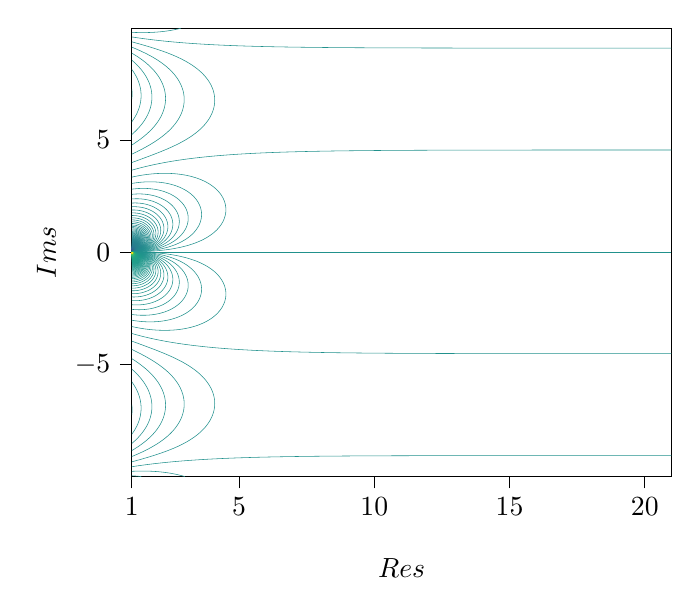
\begin{tikzpicture}

\definecolor{color0}{rgb}{0.267004,0.004874,0.329415}
\definecolor{color1}{rgb}{0.26851,0.009605,0.335427}
\definecolor{color2}{rgb}{0.269944,0.014625,0.341379}
\definecolor{color3}{rgb}{0.271305,0.019942,0.347269}
\definecolor{color4}{rgb}{0.272594,0.025563,0.353093}
\definecolor{color5}{rgb}{0.273809,0.031497,0.358853}
\definecolor{color6}{rgb}{0.274952,0.037752,0.364543}
\definecolor{color7}{rgb}{0.276022,0.044167,0.370164}
\definecolor{color8}{rgb}{0.277018,0.050344,0.375715}
\definecolor{color9}{rgb}{0.277941,0.056324,0.381191}
\definecolor{color10}{rgb}{0.278791,0.062145,0.386592}
\definecolor{color11}{rgb}{0.279566,0.067836,0.391917}
\definecolor{color12}{rgb}{0.280267,0.073417,0.397163}
\definecolor{color13}{rgb}{0.280894,0.078907,0.402329}
\definecolor{color14}{rgb}{0.281446,0.08432,0.407414}
\definecolor{color15}{rgb}{0.281924,0.089666,0.412415}
\definecolor{color16}{rgb}{0.282327,0.094955,0.417331}
\definecolor{color17}{rgb}{0.282656,0.100196,0.42216}
\definecolor{color18}{rgb}{0.28291,0.105393,0.426902}
\definecolor{color19}{rgb}{0.283091,0.110553,0.431554}
\definecolor{color20}{rgb}{0.283197,0.11568,0.436115}
\definecolor{color21}{rgb}{0.283229,0.120777,0.440584}
\definecolor{color22}{rgb}{0.283187,0.125848,0.44496}
\definecolor{color23}{rgb}{0.283072,0.130895,0.449241}
\definecolor{color24}{rgb}{0.282884,0.13592,0.453427}
\definecolor{color25}{rgb}{0.282623,0.140926,0.457517}
\definecolor{color26}{rgb}{0.28229,0.145912,0.46151}
\definecolor{color27}{rgb}{0.281887,0.150881,0.465405}
\definecolor{color28}{rgb}{0.281412,0.155834,0.469201}
\definecolor{color29}{rgb}{0.280868,0.160771,0.472899}
\definecolor{color30}{rgb}{0.280255,0.165693,0.476498}
\definecolor{color31}{rgb}{0.279574,0.170599,0.479997}
\definecolor{color32}{rgb}{0.278826,0.17549,0.483397}
\definecolor{color33}{rgb}{0.278012,0.180367,0.486697}
\definecolor{color34}{rgb}{0.277134,0.185228,0.489898}
\definecolor{color35}{rgb}{0.276194,0.190074,0.493001}
\definecolor{color36}{rgb}{0.275191,0.194905,0.496005}
\definecolor{color37}{rgb}{0.274128,0.199721,0.498911}
\definecolor{color38}{rgb}{0.273006,0.20452,0.501721}
\definecolor{color39}{rgb}{0.271828,0.209303,0.504434}
\definecolor{color40}{rgb}{0.270595,0.214069,0.507052}
\definecolor{color41}{rgb}{0.269308,0.218818,0.509577}
\definecolor{color42}{rgb}{0.267968,0.223549,0.512008}
\definecolor{color43}{rgb}{0.26658,0.228262,0.514349}
\definecolor{color44}{rgb}{0.265145,0.232956,0.516599}
\definecolor{color45}{rgb}{0.263663,0.237631,0.518762}
\definecolor{color46}{rgb}{0.262138,0.242286,0.520837}
\definecolor{color47}{rgb}{0.260571,0.246922,0.522828}
\definecolor{color48}{rgb}{0.258965,0.251537,0.524736}
\definecolor{color49}{rgb}{0.257322,0.25613,0.526563}
\definecolor{color50}{rgb}{0.255645,0.260703,0.528312}
\definecolor{color51}{rgb}{0.253935,0.265254,0.529983}
\definecolor{color52}{rgb}{0.252194,0.269783,0.531579}
\definecolor{color53}{rgb}{0.250425,0.27429,0.533103}
\definecolor{color54}{rgb}{0.248629,0.278775,0.534556}
\definecolor{color55}{rgb}{0.246811,0.283237,0.535941}
\definecolor{color56}{rgb}{0.244972,0.287675,0.53726}
\definecolor{color57}{rgb}{0.243113,0.292092,0.538516}
\definecolor{color58}{rgb}{0.241237,0.296485,0.539709}
\definecolor{color59}{rgb}{0.239346,0.300855,0.540844}
\definecolor{color60}{rgb}{0.237441,0.305202,0.541921}
\definecolor{color61}{rgb}{0.235526,0.309527,0.542944}
\definecolor{color62}{rgb}{0.233603,0.313828,0.543914}
\definecolor{color63}{rgb}{0.231674,0.318106,0.544834}
\definecolor{color64}{rgb}{0.229739,0.322361,0.545706}
\definecolor{color65}{rgb}{0.227802,0.326594,0.546532}
\definecolor{color66}{rgb}{0.225863,0.330805,0.547314}
\definecolor{color67}{rgb}{0.223925,0.334994,0.548053}
\definecolor{color68}{rgb}{0.221989,0.339161,0.548752}
\definecolor{color69}{rgb}{0.220057,0.343307,0.549413}
\definecolor{color70}{rgb}{0.21813,0.347432,0.550038}
\definecolor{color71}{rgb}{0.21621,0.351535,0.550627}
\definecolor{color72}{rgb}{0.214298,0.355619,0.551184}
\definecolor{color73}{rgb}{0.212395,0.359683,0.55171}
\definecolor{color74}{rgb}{0.210503,0.363727,0.552206}
\definecolor{color75}{rgb}{0.208623,0.367752,0.552675}
\definecolor{color76}{rgb}{0.206756,0.371758,0.553117}
\definecolor{color77}{rgb}{0.204903,0.375746,0.553533}
\definecolor{color78}{rgb}{0.203063,0.379716,0.553925}
\definecolor{color79}{rgb}{0.201239,0.38367,0.554294}
\definecolor{color80}{rgb}{0.19943,0.387607,0.554642}
\definecolor{color81}{rgb}{0.197636,0.391528,0.554969}
\definecolor{color82}{rgb}{0.19586,0.395433,0.555276}
\definecolor{color83}{rgb}{0.1941,0.399323,0.555565}
\definecolor{color84}{rgb}{0.192357,0.403199,0.555836}
\definecolor{color85}{rgb}{0.190631,0.407061,0.556089}
\definecolor{color86}{rgb}{0.188923,0.41091,0.556326}
\definecolor{color87}{rgb}{0.187231,0.414746,0.556547}
\definecolor{color88}{rgb}{0.185556,0.41857,0.556753}
\definecolor{color89}{rgb}{0.183898,0.422383,0.556944}
\definecolor{color90}{rgb}{0.182256,0.426184,0.55712}
\definecolor{color91}{rgb}{0.180629,0.429975,0.557282}
\definecolor{color92}{rgb}{0.179019,0.433756,0.55743}
\definecolor{color93}{rgb}{0.177423,0.437527,0.557565}
\definecolor{color94}{rgb}{0.175841,0.44129,0.557685}
\definecolor{color95}{rgb}{0.174274,0.445044,0.557792}
\definecolor{color96}{rgb}{0.172719,0.448791,0.557885}
\definecolor{color97}{rgb}{0.171176,0.45253,0.557965}
\definecolor{color98}{rgb}{0.169646,0.456262,0.55803}
\definecolor{color99}{rgb}{0.168126,0.459988,0.558082}
\definecolor{color100}{rgb}{0.166617,0.463708,0.558119}
\definecolor{color101}{rgb}{0.165117,0.467423,0.558141}
\definecolor{color102}{rgb}{0.163625,0.471133,0.558148}
\definecolor{color103}{rgb}{0.162142,0.474838,0.55814}
\definecolor{color104}{rgb}{0.160665,0.47854,0.558115}
\definecolor{color105}{rgb}{0.159194,0.482237,0.558073}
\definecolor{color106}{rgb}{0.157729,0.485932,0.558013}
\definecolor{color107}{rgb}{0.15627,0.489624,0.557936}
\definecolor{color108}{rgb}{0.154815,0.493313,0.55784}
\definecolor{color109}{rgb}{0.153364,0.497,0.557724}
\definecolor{color110}{rgb}{0.151918,0.500685,0.557587}
\definecolor{color111}{rgb}{0.150476,0.504369,0.55743}
\definecolor{color112}{rgb}{0.149039,0.508051,0.55725}
\definecolor{color113}{rgb}{0.147607,0.511733,0.557049}
\definecolor{color114}{rgb}{0.14618,0.515413,0.556823}
\definecolor{color115}{rgb}{0.144759,0.519093,0.556572}
\definecolor{color116}{rgb}{0.143343,0.522773,0.556295}
\definecolor{color117}{rgb}{0.141935,0.526453,0.555991}
\definecolor{color118}{rgb}{0.140536,0.530132,0.555659}
\definecolor{color119}{rgb}{0.139147,0.533812,0.555298}
\definecolor{color120}{rgb}{0.13777,0.537492,0.554906}
\definecolor{color121}{rgb}{0.136408,0.541173,0.554483}
\definecolor{color122}{rgb}{0.135066,0.544853,0.554029}
\definecolor{color123}{rgb}{0.133743,0.548535,0.553541}
\definecolor{color124}{rgb}{0.132444,0.552216,0.553018}
\definecolor{color125}{rgb}{0.131172,0.555899,0.552459}
\definecolor{color126}{rgb}{0.129933,0.559582,0.551864}
\definecolor{color127}{rgb}{0.128729,0.563265,0.551229}
\definecolor{color128}{rgb}{0.127568,0.566949,0.550556}
\definecolor{color129}{rgb}{0.126453,0.570633,0.549841}
\definecolor{color130}{rgb}{0.125394,0.574318,0.549086}
\definecolor{color131}{rgb}{0.124395,0.578002,0.548287}
\definecolor{color132}{rgb}{0.123463,0.581687,0.547445}
\definecolor{color133}{rgb}{0.122606,0.585371,0.546557}
\definecolor{color134}{rgb}{0.121831,0.589055,0.545623}
\definecolor{color135}{rgb}{0.121148,0.592739,0.544641}
\definecolor{color136}{rgb}{0.120565,0.596422,0.543611}
\definecolor{color137}{rgb}{0.120092,0.600104,0.54253}
\definecolor{color138}{rgb}{0.119738,0.603785,0.5414}
\definecolor{color139}{rgb}{0.119512,0.607464,0.540218}
\definecolor{color140}{rgb}{0.119423,0.611141,0.538982}
\definecolor{color141}{rgb}{0.119483,0.614817,0.537692}
\definecolor{color142}{rgb}{0.119699,0.61849,0.536347}
\definecolor{color143}{rgb}{0.120081,0.622161,0.534946}
\definecolor{color144}{rgb}{0.120638,0.625828,0.533488}
\definecolor{color145}{rgb}{0.12138,0.629492,0.531973}
\definecolor{color146}{rgb}{0.122312,0.633153,0.530398}
\definecolor{color147}{rgb}{0.123444,0.636809,0.528763}
\definecolor{color148}{rgb}{0.12478,0.640461,0.527068}
\definecolor{color149}{rgb}{0.126326,0.644107,0.525311}
\definecolor{color150}{rgb}{0.128087,0.647749,0.523491}
\definecolor{color151}{rgb}{0.130067,0.651384,0.521608}
\definecolor{color152}{rgb}{0.132268,0.655014,0.519661}
\definecolor{color153}{rgb}{0.134692,0.658636,0.517649}
\definecolor{color154}{rgb}{0.137339,0.662252,0.515571}
\definecolor{color155}{rgb}{0.14021,0.665859,0.513427}
\definecolor{color156}{rgb}{0.143303,0.669459,0.511215}
\definecolor{color157}{rgb}{0.146616,0.67305,0.508936}
\definecolor{color158}{rgb}{0.150148,0.676631,0.506589}
\definecolor{color159}{rgb}{0.153894,0.680203,0.504172}
\definecolor{color160}{rgb}{0.157851,0.683765,0.501686}
\definecolor{color161}{rgb}{0.162016,0.687316,0.499129}
\definecolor{color162}{rgb}{0.166383,0.690856,0.496502}
\definecolor{color163}{rgb}{0.170948,0.694384,0.493803}
\definecolor{color164}{rgb}{0.175707,0.6979,0.491033}
\definecolor{color165}{rgb}{0.180653,0.701402,0.488189}
\definecolor{color166}{rgb}{0.185783,0.704891,0.485273}
\definecolor{color167}{rgb}{0.19109,0.708366,0.482284}
\definecolor{color168}{rgb}{0.196571,0.711827,0.479221}
\definecolor{color169}{rgb}{0.202219,0.715272,0.476084}
\definecolor{color170}{rgb}{0.20803,0.718701,0.472873}
\definecolor{color171}{rgb}{0.214,0.722114,0.469588}
\definecolor{color172}{rgb}{0.220124,0.725509,0.466226}
\definecolor{color173}{rgb}{0.226397,0.728888,0.462789}
\definecolor{color174}{rgb}{0.232815,0.732247,0.459277}
\definecolor{color175}{rgb}{0.239374,0.735588,0.455688}
\definecolor{color176}{rgb}{0.24607,0.73891,0.452024}
\definecolor{color177}{rgb}{0.252899,0.742211,0.448284}
\definecolor{color178}{rgb}{0.259857,0.745492,0.444467}
\definecolor{color179}{rgb}{0.266941,0.748751,0.440573}
\definecolor{color180}{rgb}{0.274149,0.751988,0.436601}
\definecolor{color181}{rgb}{0.281477,0.755203,0.432552}
\definecolor{color182}{rgb}{0.288921,0.758394,0.428426}
\definecolor{color183}{rgb}{0.296479,0.761561,0.424223}
\definecolor{color184}{rgb}{0.304148,0.764704,0.419943}
\definecolor{color185}{rgb}{0.311925,0.767822,0.415586}
\definecolor{color186}{rgb}{0.319809,0.770914,0.411152}
\definecolor{color187}{rgb}{0.327796,0.77398,0.40664}
\definecolor{color188}{rgb}{0.335885,0.777018,0.402049}
\definecolor{color189}{rgb}{0.344074,0.780029,0.397381}
\definecolor{color190}{rgb}{0.35236,0.783011,0.392636}
\definecolor{color191}{rgb}{0.360741,0.785964,0.387814}
\definecolor{color192}{rgb}{0.369214,0.788888,0.382914}
\definecolor{color193}{rgb}{0.377779,0.791781,0.377939}
\definecolor{color194}{rgb}{0.386433,0.794644,0.372886}
\definecolor{color195}{rgb}{0.395174,0.797475,0.367757}
\definecolor{color196}{rgb}{0.404001,0.800275,0.362552}
\definecolor{color197}{rgb}{0.412913,0.803041,0.357269}
\definecolor{color198}{rgb}{0.421908,0.805774,0.35191}
\definecolor{color199}{rgb}{0.430983,0.808473,0.346476}
\definecolor{color200}{rgb}{0.440137,0.811138,0.340967}
\definecolor{color201}{rgb}{0.449368,0.813768,0.335384}
\definecolor{color202}{rgb}{0.458674,0.816363,0.329727}
\definecolor{color203}{rgb}{0.468053,0.818921,0.323998}
\definecolor{color204}{rgb}{0.477504,0.821444,0.318195}
\definecolor{color205}{rgb}{0.487026,0.823929,0.312321}
\definecolor{color206}{rgb}{0.496615,0.826376,0.306377}
\definecolor{color207}{rgb}{0.506271,0.828786,0.300362}
\definecolor{color208}{rgb}{0.515992,0.831158,0.294279}
\definecolor{color209}{rgb}{0.525776,0.833491,0.288127}
\definecolor{color210}{rgb}{0.535621,0.835785,0.281908}
\definecolor{color211}{rgb}{0.545524,0.838039,0.275626}
\definecolor{color212}{rgb}{0.555484,0.840254,0.269281}
\definecolor{color213}{rgb}{0.565498,0.84243,0.262877}
\definecolor{color214}{rgb}{0.575563,0.844566,0.256415}
\definecolor{color215}{rgb}{0.585678,0.846661,0.249897}
\definecolor{color216}{rgb}{0.595839,0.848717,0.243329}
\definecolor{color217}{rgb}{0.606045,0.850733,0.236712}
\definecolor{color218}{rgb}{0.616293,0.852709,0.230052}
\definecolor{color219}{rgb}{0.626579,0.854645,0.223353}
\definecolor{color220}{rgb}{0.636902,0.856542,0.21662}
\definecolor{color221}{rgb}{0.647257,0.8584,0.209861}
\definecolor{color222}{rgb}{0.657642,0.860219,0.203082}
\definecolor{color223}{rgb}{0.668054,0.861999,0.196293}
\definecolor{color224}{rgb}{0.678489,0.863742,0.189503}
\definecolor{color225}{rgb}{0.688944,0.865448,0.182725}
\definecolor{color226}{rgb}{0.699415,0.867117,0.175971}
\definecolor{color227}{rgb}{0.709898,0.868751,0.169257}
\definecolor{color228}{rgb}{0.720391,0.87035,0.162603}
\definecolor{color229}{rgb}{0.730889,0.871916,0.156029}
\definecolor{color230}{rgb}{0.741388,0.873449,0.149561}
\definecolor{color231}{rgb}{0.751884,0.874951,0.143228}
\definecolor{color232}{rgb}{0.762373,0.876424,0.137064}
\definecolor{color233}{rgb}{0.772852,0.877868,0.131109}
\definecolor{color234}{rgb}{0.783315,0.879285,0.125405}
\definecolor{color235}{rgb}{0.79376,0.880678,0.120005}
\definecolor{color236}{rgb}{0.804182,0.882046,0.114965}
\definecolor{color237}{rgb}{0.814576,0.883393,0.110347}
\definecolor{color238}{rgb}{0.82494,0.88472,0.106217}
\definecolor{color239}{rgb}{0.83527,0.886029,0.102646}
\definecolor{color240}{rgb}{0.845561,0.887322,0.099702}
\definecolor{color241}{rgb}{0.85581,0.888601,0.097452}
\definecolor{color242}{rgb}{0.866013,0.889868,0.095953}
\definecolor{color243}{rgb}{0.876168,0.891125,0.09525}
\definecolor{color244}{rgb}{0.886271,0.892374,0.095374}
\definecolor{color245}{rgb}{0.89632,0.893616,0.096335}
\definecolor{color246}{rgb}{0.906311,0.894855,0.098125}
\definecolor{color247}{rgb}{0.916242,0.896091,0.100717}
\definecolor{color248}{rgb}{0.926106,0.89733,0.104071}
\definecolor{color249}{rgb}{0.935904,0.89857,0.108131}
\definecolor{color250}{rgb}{0.945636,0.899815,0.112838}
\definecolor{color251}{rgb}{0.9553,0.901065,0.118128}
\definecolor{color252}{rgb}{0.964894,0.902323,0.123941}
\definecolor{color253}{rgb}{0.974417,0.90359,0.130215}
\definecolor{color254}{rgb}{0.983868,0.904867,0.136897}
\definecolor{color255}{rgb}{0.993248,0.906157,0.143936}

\begin{axis}[
tick align=outside,
tick pos=left,
x grid style={white!69.0196078431373!black},
xmin=1.035, xmax=20.985,
xtick style={color=black},
y grid style={white!69.0196078431373!black},
ymin=-9.975, ymax=9.975,
ytick style={color=black},
extra x ticks = {1.035},
extra x tick labels = {$1$},
xlabel= $\operatorname{Re} s$,
ylabel = $\operatorname{Im} s$,
]
\path [draw=color0, very thin]
(axis cs:1.035,0.0751453554000022)
--(axis cs:1.03512295264031,0.0750000000000011)
--(axis cs:1.035,0.0749294402183081);

\path [draw=color0, very thin]
(axis cs:1.035,0.075413210188517)
--(axis cs:1.03534952456999,0.0750000000000011)
--(axis cs:1.035,0.0747994156344062);

\path [draw=color0, very thin]
(axis cs:1.035,0.0756810649770318)
--(axis cs:1.03557609649966,0.0750000000000011)
--(axis cs:1.035,0.0746693910505044);

\path [draw=color1, very thin]
(axis cs:1.035,0.0759489197655467)
--(axis cs:1.03580266842934,0.0750000000000011)
--(axis cs:1.035,0.0745393664666025);

\path [draw=color1, very thin]
(axis cs:1.035,0.0762167745540615)
--(axis cs:1.03602924035902,0.0750000000000011)
--(axis cs:1.035,0.0744093418827007);

\path [draw=color1, very thin]
(axis cs:1.035,0.0764846293425763)
--(axis cs:1.0362558122887,0.0750000000000011)
--(axis cs:1.035,0.0742793172987988);

\path [draw=color2, very thin]
(axis cs:1.035,0.0767524841310911)
--(axis cs:1.03648238421838,0.0750000000000011)
--(axis cs:1.035,0.074149292714897);

\path [draw=color2, very thin]
(axis cs:1.035,0.077020338919606)
--(axis cs:1.03670895614805,0.0750000000000011)
--(axis cs:1.035,0.0740192681309952);

\path [draw=color2, very thin]
(axis cs:1.035,0.0772881937081208)
--(axis cs:1.03693552807773,0.0750000000000011)
--(axis cs:1.035,0.0738892435470933);

\path [draw=color3, very thin]
(axis cs:1.035,0.0775560484966356)
--(axis cs:1.03716210000741,0.0750000000000011)
--(axis cs:1.035,0.0737592189631915);

\path [draw=color3, very thin]
(axis cs:1.035,0.0778239032851504)
--(axis cs:1.03738867193709,0.0750000000000011)
--(axis cs:1.035,0.0736291943792896);

\path [draw=color3, very thin]
(axis cs:1.035,0.0780917580736653)
--(axis cs:1.03761524386676,0.0750000000000011)
--(axis cs:1.035,0.0734991697953878);

\path [draw=color4, very thin]
(axis cs:1.035,0.0783596128621801)
--(axis cs:1.03784181579644,0.0750000000000011)
--(axis cs:1.035,0.073369145211486);

\path [draw=color4, very thin]
(axis cs:1.035,0.0786274676506949)
--(axis cs:1.03806838772612,0.0750000000000011)
--(axis cs:1.035,0.0732391206275841);

\path [draw=color4, very thin]
(axis cs:1.035,0.0788953224392097)
--(axis cs:1.0382949596558,0.0750000000000011)
--(axis cs:1.035,0.0731090960436823);

\path [draw=color5, very thin]
(axis cs:1.035,0.0791631772277246)
--(axis cs:1.03852153158548,0.0750000000000011)
--(axis cs:1.035,0.0729790714597804);

\path [draw=color5, very thin]
(axis cs:1.035,0.0794310320162394)
--(axis cs:1.03874810351515,0.0750000000000011)
--(axis cs:1.035,0.0728490468758786);

\path [draw=color5, very thin]
(axis cs:1.035,0.0796988868047542)
--(axis cs:1.03897467544483,0.0750000000000011)
--(axis cs:1.035,0.0727190222919767);

\path [draw=color6, very thin]
(axis cs:1.035,0.079966741593269)
--(axis cs:1.03920124737451,0.0750000000000011)
--(axis cs:1.035,0.0725889977080749);

\path [draw=color6, very thin]
(axis cs:1.035,0.0802345963817839)
--(axis cs:1.03942781930419,0.0750000000000011)
--(axis cs:1.035,0.072458973124173);

\path [draw=color6, very thin]
(axis cs:1.035,0.0805024511702987)
--(axis cs:1.03965439123386,0.0750000000000011)
--(axis cs:1.035,0.0723289485402712);

\path [draw=color7, very thin]
(axis cs:1.035,0.0807703059588135)
--(axis cs:1.03988096316354,0.0750000000000011)
--(axis cs:1.035,0.0721989239563694);

\path [draw=color7, very thin]
(axis cs:1.035,0.0810381607473283)
--(axis cs:1.04010753509322,0.0750000000000011)
--(axis cs:1.035,0.0720688993724675);

\path [draw=color7, very thin]
(axis cs:1.035,0.0813060155358432)
--(axis cs:1.0403341070229,0.0750000000000011)
--(axis cs:1.035,0.0719388747885657);

\path [draw=color8, very thin]
(axis cs:1.035,0.081573870324358)
--(axis cs:1.04056067895258,0.0750000000000011)
--(axis cs:1.035,0.0718088502046638);

\path [draw=color8, very thin]
(axis cs:1.035,0.0818417251128728)
--(axis cs:1.04078725088225,0.0750000000000011)
--(axis cs:1.035,0.071678825620762);

\path [draw=color8, very thin]
(axis cs:1.035,0.0821095799013876)
--(axis cs:1.04101382281193,0.0750000000000011)
--(axis cs:1.035,0.0715488010368601);

\path [draw=color9, very thin]
(axis cs:1.035,0.0823774346899025)
--(axis cs:1.04124039474161,0.0750000000000011)
--(axis cs:1.035,0.0714187764529583);

\path [draw=color9, very thin]
(axis cs:1.035,0.0826452894784173)
--(axis cs:1.04146696667129,0.0750000000000011)
--(axis cs:1.035,0.0712887518690565);

\path [draw=color9, very thin]
(axis cs:1.035,0.0829131442669321)
--(axis cs:1.04169353860096,0.0750000000000011)
--(axis cs:1.035,0.0711587272851546);

\path [draw=color10, very thin]
(axis cs:1.035,0.0831809990554469)
--(axis cs:1.04192011053064,0.0750000000000011)
--(axis cs:1.035,0.0710287027012528);

\path [draw=color10, very thin]
(axis cs:1.035,0.0834488538439618)
--(axis cs:1.04214668246032,0.0750000000000011)
--(axis cs:1.035,0.0708986781173509);

\path [draw=color10, very thin]
(axis cs:1.035,0.0837167086324766)
--(axis cs:1.04237325439,0.0750000000000011)
--(axis cs:1.035,0.0707686535334491);

\path [draw=color11, very thin]
(axis cs:1.035,0.0839845634209914)
--(axis cs:1.04259982631968,0.0750000000000011)
--(axis cs:1.035,0.0706386289495472);

\path [draw=color11, very thin]
(axis cs:1.035,0.0842524182095062)
--(axis cs:1.04282639824935,0.0750000000000011)
--(axis cs:1.035,0.0705086043656454);

\path [draw=color11, very thin]
(axis cs:1.035,0.0845202729980211)
--(axis cs:1.04305297017903,0.0750000000000011)
--(axis cs:1.035,0.0703785797817436);

\path [draw=color12, very thin]
(axis cs:1.035,0.0847881277865359)
--(axis cs:1.04327954210871,0.0750000000000011)
--(axis cs:1.035,0.0702485551978417);

\path [draw=color12, very thin]
(axis cs:1.035,0.0850559825750507)
--(axis cs:1.04350611403839,0.0750000000000011)
--(axis cs:1.035,0.0701185306139399);

\path [draw=color12, very thin]
(axis cs:1.035,0.0853238373635655)
--(axis cs:1.04373268596806,0.0750000000000011)
--(axis cs:1.035,0.069988506030038);

\path [draw=color13, very thin]
(axis cs:1.035,0.0855916921520804)
--(axis cs:1.04395925789774,0.0750000000000011)
--(axis cs:1.035,0.0698584814461362);

\path [draw=color13, very thin]
(axis cs:1.035,0.0858595469405952)
--(axis cs:1.04418582982742,0.0750000000000011)
--(axis cs:1.035,0.0697284568622343);

\path [draw=color13, very thin]
(axis cs:1.035,0.08612740172911)
--(axis cs:1.0444124017571,0.0750000000000011)
--(axis cs:1.035,0.0695984322783325);

\path [draw=color14, very thin]
(axis cs:1.035,0.0863952565176248)
--(axis cs:1.04463897368677,0.0750000000000011)
--(axis cs:1.035,0.0694684076944306);

\path [draw=color14, very thin]
(axis cs:1.035,0.0866631113061397)
--(axis cs:1.04486554561645,0.0750000000000011)
--(axis cs:1.035,0.0693383831105288);

\path [draw=color14, very thin]
(axis cs:1.035,0.0869309660946545)
--(axis cs:1.04509211754613,0.0750000000000011)
--(axis cs:1.035,0.069208358526627);

\path [draw=color15, very thin]
(axis cs:1.035,0.0871988208831693)
--(axis cs:1.04531868947581,0.0750000000000011)
--(axis cs:1.035,0.0690783339427251);

\path [draw=color15, very thin]
(axis cs:1.035,0.0874666756716841)
--(axis cs:1.04554526140549,0.0750000000000011)
--(axis cs:1.035,0.0689483093588233);

\path [draw=color15, very thin]
(axis cs:1.035,0.087734530460199)
--(axis cs:1.04577183333516,0.0750000000000011)
--(axis cs:1.035,0.0688182847749214);

\path [draw=color16, very thin]
(axis cs:1.035,0.0880023852487138)
--(axis cs:1.04599840526484,0.0750000000000011)
--(axis cs:1.035,0.0686882601910196);

\path [draw=color16, very thin]
(axis cs:1.035,0.0882702400372286)
--(axis cs:1.04622497719452,0.0750000000000011)
--(axis cs:1.035,0.0685582356071178);

\path [draw=color16, very thin]
(axis cs:1.035,0.0885380948257434)
--(axis cs:1.0464515491242,0.0750000000000011)
--(axis cs:1.035,0.0684282110232159);

\path [draw=color17, very thin]
(axis cs:1.035,0.0888059496142583)
--(axis cs:1.04667812105387,0.0750000000000011)
--(axis cs:1.035,0.0682981864393141);

\path [draw=color17, very thin]
(axis cs:1.035,0.0890738044027731)
--(axis cs:1.04690469298355,0.0750000000000011)
--(axis cs:1.035,0.0681681618554122);

\path [draw=color17, very thin]
(axis cs:1.035,0.0893416591912879)
--(axis cs:1.04713126491323,0.0750000000000011)
--(axis cs:1.035,0.0680381372715104);

\path [draw=color18, very thin]
(axis cs:1.035,0.0896095139798027)
--(axis cs:1.04735783684291,0.0750000000000011)
--(axis cs:1.035,0.0679081126876085);

\path [draw=color18, very thin]
(axis cs:1.035,0.0898773687683176)
--(axis cs:1.04758440877259,0.0750000000000011)
--(axis cs:1.035,0.0677780881037067);

\path [draw=color18, very thin]
(axis cs:1.035,0.0901452235568324)
--(axis cs:1.04781098070226,0.0750000000000011)
--(axis cs:1.035,0.0676480635198048);

\path [draw=color19, very thin]
(axis cs:1.035,0.0904130783453472)
--(axis cs:1.04803755263194,0.0750000000000011)
--(axis cs:1.035,0.067518038935903);

\path [draw=color19, very thin]
(axis cs:1.035,0.090680933133862)
--(axis cs:1.04826412456162,0.0750000000000011)
--(axis cs:1.035,0.0673880143520012);

\path [draw=color19, very thin]
(axis cs:1.035,0.0909487879223769)
--(axis cs:1.0484906964913,0.0750000000000011)
--(axis cs:1.035,0.0672579897680993);

\path [draw=color20, very thin]
(axis cs:1.035,0.0912166427108917)
--(axis cs:1.04871726842097,0.0750000000000011)
--(axis cs:1.035,0.0671279651841975);

\path [draw=color20, very thin]
(axis cs:1.035,0.0914844974994065)
--(axis cs:1.04894384035065,0.0750000000000011)
--(axis cs:1.035,0.0669979406002956);

\path [draw=color20, very thin]
(axis cs:1.035,0.0917523522879213)
--(axis cs:1.04917041228033,0.0750000000000011)
--(axis cs:1.035,0.0668679160163938);

\path [draw=color21, very thin]
(axis cs:1.035,0.0920202070764362)
--(axis cs:1.04939698421001,0.0750000000000011)
--(axis cs:1.035,0.066737891432492);

\path [draw=color21, very thin]
(axis cs:1.035,0.092288061864951)
--(axis cs:1.04962355613969,0.0750000000000011)
--(axis cs:1.035,0.0666078668485901);

\path [draw=color21, very thin]
(axis cs:1.035,0.0925559166534658)
--(axis cs:1.04985012806936,0.0750000000000011)
--(axis cs:1.035,0.0664778422646883);

\path [draw=color22, very thin]
(axis cs:1.035,0.0928237714419806)
--(axis cs:1.05007669999904,0.0750000000000011)
--(axis cs:1.035,0.0663478176807864);

\path [draw=color22, very thin]
(axis cs:1.035,0.0930916262304955)
--(axis cs:1.05030327192872,0.0750000000000011)
--(axis cs:1.035,0.0662177930968846);

\path [draw=color22, very thin]
(axis cs:1.035,0.0933594810190103)
--(axis cs:1.0505298438584,0.0750000000000011)
--(axis cs:1.035,0.0660877685129827);

\path [draw=color23, very thin]
(axis cs:1.035,0.0936273358075251)
--(axis cs:1.05075641578807,0.0750000000000011)
--(axis cs:1.035,0.0659577439290809);

\path [draw=color23, very thin]
(axis cs:1.035,0.0938951905960399)
--(axis cs:1.05098298771775,0.0750000000000011)
--(axis cs:1.035,0.065827719345179);

\path [draw=color23, very thin]
(axis cs:1.035,0.0941630453845547)
--(axis cs:1.05120955964743,0.0750000000000011)
--(axis cs:1.035,0.0656976947612772);

\path [draw=color24, very thin]
(axis cs:1.035,0.0944309001730696)
--(axis cs:1.05143613157711,0.0750000000000011)
--(axis cs:1.035,0.0655676701773754);

\path [draw=color24, very thin]
(axis cs:1.035,0.0946987549615844)
--(axis cs:1.05166270350679,0.0750000000000011)
--(axis cs:1.035,0.0654376455934735);

\path [draw=color24, very thin]
(axis cs:1.035,0.0949666097500992)
--(axis cs:1.05188927543646,0.0750000000000011)
--(axis cs:1.035,0.0653076210095717);

\path [draw=color25, very thin]
(axis cs:1.035,0.0952344645386141)
--(axis cs:1.05211584736614,0.0750000000000011)
--(axis cs:1.035,0.0651775964256698);

\path [draw=color25, very thin]
(axis cs:1.035,0.0955023193271289)
--(axis cs:1.05234241929582,0.0750000000000011)
--(axis cs:1.035,0.065047571841768);

\path [draw=color25, very thin]
(axis cs:1.035,0.0957701741156437)
--(axis cs:1.0525689912255,0.0750000000000011)
--(axis cs:1.035,0.0649175472578662);

\path [draw=color26, very thin]
(axis cs:1.035,0.0960380289041585)
--(axis cs:1.05279556315517,0.0750000000000011)
--(axis cs:1.035,0.0647875226739643);

\path [draw=color26, very thin]
(axis cs:1.035,0.0963058836926733)
--(axis cs:1.05302213508485,0.0750000000000011)
--(axis cs:1.035,0.0646574980900625);

\path [draw=color26, very thin]
(axis cs:1.035,0.0965737384811882)
--(axis cs:1.05324870701453,0.0750000000000011)
--(axis cs:1.035,0.0645274735061606);

\path [draw=color27, very thin]
(axis cs:1.035,0.096841593269703)
--(axis cs:1.05347527894421,0.0750000000000011)
--(axis cs:1.035,0.0643974489222588);

\path [draw=color27, very thin]
(axis cs:1.035,0.0971094480582178)
--(axis cs:1.05370185087389,0.0750000000000011)
--(axis cs:1.035,0.0642674243383569);

\path [draw=color27, very thin]
(axis cs:1.035,0.0973773028467326)
--(axis cs:1.05392842280356,0.0750000000000011)
--(axis cs:1.035,0.0641373997544551);

\path [draw=color28, very thin]
(axis cs:1.035,0.0976451576352475)
--(axis cs:1.05415499473324,0.0750000000000011)
--(axis cs:1.035,0.0640073751705532);

\path [draw=color28, very thin]
(axis cs:1.035,0.0979130124237623)
--(axis cs:1.05438156666292,0.0750000000000011)
--(axis cs:1.035,0.0638773505866514);

\path [draw=color28, very thin]
(axis cs:1.035,0.0981808672122771)
--(axis cs:1.0546081385926,0.0750000000000011)
--(axis cs:1.035,0.0637473260027496);

\path [draw=color29, very thin]
(axis cs:1.035,0.0984487220007919)
--(axis cs:1.05483471052227,0.0750000000000011)
--(axis cs:1.035,0.0636173014188477);

\path [draw=color29, very thin]
(axis cs:1.035,0.0987165767893068)
--(axis cs:1.05506128245195,0.0750000000000011)
--(axis cs:1.035,0.0634872768349459);

\path [draw=color29, very thin]
(axis cs:1.035,0.0989844315778216)
--(axis cs:1.05528785438163,0.0750000000000011)
--(axis cs:1.035,0.063357252251044);

\path [draw=color30, very thin]
(axis cs:1.035,0.0992522863663364)
--(axis cs:1.05551442631131,0.0750000000000011)
--(axis cs:1.035,0.0632272276671422);

\path [draw=color30, very thin]
(axis cs:1.035,0.0995201411548512)
--(axis cs:1.05574099824099,0.0750000000000011)
--(axis cs:1.035,0.0630972030832403);

\path [draw=color30, very thin]
(axis cs:1.035,0.0997879959433661)
--(axis cs:1.05596757017066,0.0750000000000011)
--(axis cs:1.035,0.0629671784993385);

\path [draw=color31, very thin]
(axis cs:1.035,0.100055850731881)
--(axis cs:1.05619414210034,0.0750000000000011)
--(axis cs:1.035,0.0628371539154367);

\path [draw=color31, very thin]
(axis cs:1.035,0.100323705520396)
--(axis cs:1.05642071403002,0.0750000000000011)
--(axis cs:1.035,0.0627071293315348);

\path [draw=color31, very thin]
(axis cs:1.035,0.100591560308911)
--(axis cs:1.0566472859597,0.0750000000000011)
--(axis cs:1.035,0.062577104747633);

\path [draw=color32, very thin]
(axis cs:1.035,0.100859415097425)
--(axis cs:1.05687385788937,0.0750000000000011)
--(axis cs:1.035,0.0624470801637311);

\path [draw=color32, very thin]
(axis cs:1.035,0.10112726988594)
--(axis cs:1.05710042981905,0.0750000000000011)
--(axis cs:1.035,0.0623170555798293);

\path [draw=color32, very thin]
(axis cs:1.035,0.101395124674455)
--(axis cs:1.05732700174873,0.0750000000000011)
--(axis cs:1.035,0.0621870309959274);

\path [draw=color33, very thin]
(axis cs:1.035,0.10166297946297)
--(axis cs:1.05755357367841,0.0750000000000011)
--(axis cs:1.035,0.0620570064120256);

\path [draw=color33, very thin]
(axis cs:1.035,0.101930834251485)
--(axis cs:1.05778014560809,0.0750000000000011)
--(axis cs:1.035,0.0619269818281238);

\path [draw=color33, very thin]
(axis cs:1.035,0.10219868904)
--(axis cs:1.05800671753776,0.0750000000000011)
--(axis cs:1.035,0.0617969572442219);

\path [draw=color34, very thin]
(axis cs:1.035,0.102466543828514)
--(axis cs:1.05823328946744,0.0750000000000011)
--(axis cs:1.035,0.0616669326603201);

\path [draw=color34, very thin]
(axis cs:1.035,0.102734398617029)
--(axis cs:1.05845986139712,0.0750000000000011)
--(axis cs:1.035,0.0615369080764182);

\path [draw=color34, very thin]
(axis cs:1.035,0.103002253405544)
--(axis cs:1.0586864333268,0.0750000000000011)
--(axis cs:1.035,0.0614068834925164);

\path [draw=color35, very thin]
(axis cs:1.035,0.103270108194059)
--(axis cs:1.05891300525647,0.0750000000000011)
--(axis cs:1.035,0.0612768589086145);

\path [draw=color35, very thin]
(axis cs:1.035,0.103537962982574)
--(axis cs:1.05913957718615,0.0750000000000011)
--(axis cs:1.035,0.0611468343247127);

\path [draw=color35, very thin]
(axis cs:1.035,0.103805817771088)
--(axis cs:1.05936614911583,0.0750000000000011)
--(axis cs:1.035,0.0610168097408109);

\path [draw=color36, very thin]
(axis cs:1.035,0.104073672559603)
--(axis cs:1.05959272104551,0.0750000000000011)
--(axis cs:1.035,0.060886785156909);

\path [draw=color36, very thin]
(axis cs:1.035,0.104341527348118)
--(axis cs:1.05981929297519,0.0750000000000011)
--(axis cs:1.035,0.0607567605730072);

\path [draw=color36, very thin]
(axis cs:1.035,0.104609382136633)
--(axis cs:1.06004586490486,0.0750000000000011)
--(axis cs:1.035,0.0606267359891053);

\path [draw=color37, very thin]
(axis cs:1.035,0.104877236925148)
--(axis cs:1.06027243683454,0.0750000000000011)
--(axis cs:1.035,0.0604967114052035);

\path [draw=color37, very thin]
(axis cs:1.035,0.105145091713663)
--(axis cs:1.06049900876422,0.0750000000000011)
--(axis cs:1.035,0.0603666868213016);

\path [draw=color37, very thin]
(axis cs:1.035,0.105412946502177)
--(axis cs:1.0607255806939,0.0750000000000011)
--(axis cs:1.035,0.0602366622373998);

\path [draw=color38, very thin]
(axis cs:1.035,0.105680801290692)
--(axis cs:1.06095215262357,0.0750000000000011)
--(axis cs:1.035,0.060106637653498);

\path [draw=color38, very thin]
(axis cs:1.035,0.105948656079207)
--(axis cs:1.06117872455325,0.0750000000000011)
--(axis cs:1.035,0.0599766130695961);

\path [draw=color38, very thin]
(axis cs:1.035,0.106216510867722)
--(axis cs:1.06140529648293,0.0750000000000011)
--(axis cs:1.035,0.0598465884856943);

\path [draw=color39, very thin]
(axis cs:1.035,0.106484365656237)
--(axis cs:1.06163186841261,0.0750000000000011)
--(axis cs:1.035,0.0597165639017924);

\path [draw=color39, very thin]
(axis cs:1.035,0.106752220444752)
--(axis cs:1.06185844034228,0.0750000000000011)
--(axis cs:1.035,0.0595865393178906);

\path [draw=color39, very thin]
(axis cs:1.035,0.107020075233266)
--(axis cs:1.06208501227196,0.0750000000000011)
--(axis cs:1.035,0.0594565147339887);

\path [draw=color40, very thin]
(axis cs:1.035,0.107287930021781)
--(axis cs:1.06231158420164,0.0750000000000011)
--(axis cs:1.035,0.0593264901500869);

\path [draw=color40, very thin]
(axis cs:1.035,0.107555784810296)
--(axis cs:1.06253815613132,0.0750000000000011)
--(axis cs:1.035,0.0591964655661851);

\path [draw=color40, very thin]
(axis cs:1.035,0.107823639598811)
--(axis cs:1.062764728061,0.0750000000000011)
--(axis cs:1.035,0.0590664409822832);

\path [draw=color41, very thin]
(axis cs:1.035,0.108091494387326)
--(axis cs:1.06299129999067,0.0750000000000011)
--(axis cs:1.035,0.0589364163983814);

\path [draw=color41, very thin]
(axis cs:1.035,0.10835934917584)
--(axis cs:1.06321787192035,0.0750000000000011)
--(axis cs:1.035,0.0588063918144795);

\path [draw=color41, very thin]
(axis cs:1.035,0.108627203964355)
--(axis cs:1.06344444385003,0.0750000000000011)
--(axis cs:1.035,0.0586763672305777);

\path [draw=color42, very thin]
(axis cs:1.035,0.10889505875287)
--(axis cs:1.06367101577971,0.0750000000000011)
--(axis cs:1.035,0.0585463426466758);

\path [draw=color42, very thin]
(axis cs:1.035,0.109162913541385)
--(axis cs:1.06389758770938,0.0750000000000011)
--(axis cs:1.035,0.058416318062774);

\path [draw=color42, very thin]
(axis cs:1.035,0.1094307683299)
--(axis cs:1.06412415963906,0.0750000000000011)
--(axis cs:1.035,0.0582862934788722);

\path [draw=color43, very thin]
(axis cs:1.035,0.109698623118415)
--(axis cs:1.06435073156874,0.0750000000000011)
--(axis cs:1.035,0.0581562688949703);

\path [draw=color43, very thin]
(axis cs:1.035,0.109966477906929)
--(axis cs:1.06457730349842,0.0750000000000011)
--(axis cs:1.035,0.0580262443110685);

\path [draw=color43, very thin]
(axis cs:1.035,0.110234332695444)
--(axis cs:1.0648038754281,0.0750000000000011)
--(axis cs:1.035,0.0578962197271666);

\path [draw=color44, very thin]
(axis cs:1.035,0.110502187483959)
--(axis cs:1.06503044735777,0.0750000000000011)
--(axis cs:1.035,0.0577661951432648);

\path [draw=color44, very thin]
(axis cs:1.035,0.110770042272474)
--(axis cs:1.06525701928745,0.0750000000000011)
--(axis cs:1.035,0.0576361705593629);

\path [draw=color44, very thin]
(axis cs:1.035,0.111037897060989)
--(axis cs:1.06548359121713,0.0750000000000011)
--(axis cs:1.035,0.0575061459754611);

\path [draw=color45, very thin]
(axis cs:1.035,0.111305751849504)
--(axis cs:1.06571016314681,0.0750000000000011)
--(axis cs:1.035,0.0573761213915593);

\path [draw=color45, very thin]
(axis cs:1.035,0.111573606638018)
--(axis cs:1.06593673507648,0.0750000000000011)
--(axis cs:1.035,0.0572460968076574);

\path [draw=color45, very thin]
(axis cs:1.035,0.111841461426533)
--(axis cs:1.06616330700616,0.0750000000000011)
--(axis cs:1.035,0.0571160722237556);

\path [draw=color46, very thin]
(axis cs:1.035,0.112109316215048)
--(axis cs:1.06638987893584,0.0750000000000011)
--(axis cs:1.035,0.0569860476398537);

\path [draw=color46, very thin]
(axis cs:1.035,0.112377171003563)
--(axis cs:1.06661645086552,0.0750000000000011)
--(axis cs:1.035,0.0568560230559519);

\path [draw=color46, very thin]
(axis cs:1.035,0.112645025792078)
--(axis cs:1.0668430227952,0.0750000000000011)
--(axis cs:1.035,0.05672599847205);

\path [draw=color47, very thin]
(axis cs:1.035,0.112912880580592)
--(axis cs:1.06706959472487,0.0750000000000011)
--(axis cs:1.035,0.0565959738881482);

\path [draw=color47, very thin]
(axis cs:1.035,0.113180735369107)
--(axis cs:1.06729616665455,0.0750000000000011)
--(axis cs:1.035,0.0564659493042464);

\path [draw=color47, very thin]
(axis cs:1.035,0.113448590157622)
--(axis cs:1.06752273858423,0.0750000000000011)
--(axis cs:1.035,0.0563359247203445);

\path [draw=color48, very thin]
(axis cs:1.035,0.113716444946137)
--(axis cs:1.06774931051391,0.0750000000000011)
--(axis cs:1.035,0.0562059001364427);

\path [draw=color48, very thin]
(axis cs:1.035,0.113984299734652)
--(axis cs:1.06797588244358,0.0750000000000011)
--(axis cs:1.035,0.0560758755525408);

\path [draw=color48, very thin]
(axis cs:1.035,0.114252154523167)
--(axis cs:1.06820245437326,0.0750000000000011)
--(axis cs:1.035,0.055945850968639);

\path [draw=color49, very thin]
(axis cs:1.035,0.114520009311681)
--(axis cs:1.06842902630294,0.0750000000000011)
--(axis cs:1.035,0.0558158263847371);

\path [draw=color49, very thin]
(axis cs:1.035,0.114787864100196)
--(axis cs:1.06865559823262,0.0750000000000011)
--(axis cs:1.035,0.0556858018008353);

\path [draw=color49, very thin]
(axis cs:1.035,0.115055718888711)
--(axis cs:1.0688821701623,0.0750000000000011)
--(axis cs:1.035,0.0555557772169335);

\path [draw=color50, very thin]
(axis cs:1.035,0.115323573677226)
--(axis cs:1.06910874209197,0.0750000000000011)
--(axis cs:1.035,0.0554257526330316);

\path [draw=color50, very thin]
(axis cs:1.035,0.115591428465741)
--(axis cs:1.06933531402165,0.0750000000000011)
--(axis cs:1.035,0.0552957280491298);

\path [draw=color50, very thin]
(axis cs:1.035,0.115859283254256)
--(axis cs:1.06956188595133,0.0750000000000011)
--(axis cs:1.035,0.0551657034652279);

\path [draw=color51, very thin]
(axis cs:1.035,0.11612713804277)
--(axis cs:1.06978845788101,0.0750000000000011)
--(axis cs:1.035,0.0550356788813261);

\path [draw=color51, very thin]
(axis cs:1.035,0.116394992831285)
--(axis cs:1.07001502981068,0.0750000000000011)
--(axis cs:1.035,0.0549056542974242);

\path [draw=color51, very thin]
(axis cs:1.035,0.1166628476198)
--(axis cs:1.07024160174036,0.0750000000000011)
--(axis cs:1.035,0.0547756297135224);

\path [draw=color52, very thin]
(axis cs:1.035,0.116930702408315)
--(axis cs:1.07046817367004,0.0750000000000011)
--(axis cs:1.035,0.0546456051296206);

\path [draw=color52, very thin]
(axis cs:1.035,0.11719855719683)
--(axis cs:1.07069474559972,0.0750000000000011)
--(axis cs:1.035,0.0545155805457187);

\path [draw=color52, very thin]
(axis cs:1.035,0.117466411985345)
--(axis cs:1.0709213175294,0.0750000000000011)
--(axis cs:1.035,0.0543855559618169);

\path [draw=color53, very thin]
(axis cs:1.035,0.117734266773859)
--(axis cs:1.07114788945907,0.0750000000000011)
--(axis cs:1.035,0.054255531377915);

\path [draw=color53, very thin]
(axis cs:1.035,0.118002121562374)
--(axis cs:1.07137446138875,0.0750000000000011)
--(axis cs:1.035,0.0541255067940132);

\path [draw=color53, very thin]
(axis cs:1.035,0.118269976350889)
--(axis cs:1.07160103331843,0.0750000000000011)
--(axis cs:1.035,0.0539954822101113);

\path [draw=color54, very thin]
(axis cs:1.035,0.118537831139404)
--(axis cs:1.07182760524811,0.0750000000000011)
--(axis cs:1.035,0.0538654576262095);

\path [draw=color54, very thin]
(axis cs:1.035,0.118805685927919)
--(axis cs:1.07205417717778,0.0750000000000011)
--(axis cs:1.035,0.0537354330423076);

\path [draw=color54, very thin]
(axis cs:1.035,0.119073540716433)
--(axis cs:1.07228074910746,0.0750000000000011)
--(axis cs:1.035,0.0536054084584058);

\path [draw=color55, very thin]
(axis cs:1.035,0.119341395504948)
--(axis cs:1.07250732103714,0.0750000000000011)
--(axis cs:1.035,0.053475383874504);

\path [draw=color55, very thin]
(axis cs:1.035,0.119609250293463)
--(axis cs:1.07273389296682,0.0750000000000011)
--(axis cs:1.035,0.0533453592906021);

\path [draw=color55, very thin]
(axis cs:1.035,0.119877105081978)
--(axis cs:1.07296046489649,0.0750000000000011)
--(axis cs:1.035,0.0532153347067003);

\path [draw=color56, very thin]
(axis cs:1.035,0.120144959870493)
--(axis cs:1.07318703682617,0.0750000000000011)
--(axis cs:1.035,0.0530853101227984);

\path [draw=color56, very thin]
(axis cs:1.035,0.120412814659008)
--(axis cs:1.07341360875585,0.0750000000000011)
--(axis cs:1.035,0.0529552855388966);

\path [draw=color56, very thin]
(axis cs:1.035,0.120680669447522)
--(axis cs:1.07364018068553,0.0750000000000011)
--(axis cs:1.035,0.0528252609549948);

\path [draw=color57, very thin]
(axis cs:1.035,0.120948524236037)
--(axis cs:1.07386675261521,0.0750000000000011)
--(axis cs:1.035,0.0526952363710929);

\path [draw=color57, very thin]
(axis cs:1.035,0.121216379024552)
--(axis cs:1.07409332454488,0.0750000000000011)
--(axis cs:1.035,0.0525652117871911);

\path [draw=color57, very thin]
(axis cs:1.035,0.121484233813067)
--(axis cs:1.07431989647456,0.0750000000000011)
--(axis cs:1.035,0.0524351872032892);

\path [draw=color58, very thin]
(axis cs:1.035,0.121752088601582)
--(axis cs:1.07454646840424,0.0750000000000011)
--(axis cs:1.035,0.0523051626193874);

\path [draw=color58, very thin]
(axis cs:1.035,0.122019943390097)
--(axis cs:1.07477304033392,0.0750000000000011)
--(axis cs:1.035,0.0521751380354855);

\path [draw=color58, very thin]
(axis cs:1.035,0.122287798178611)
--(axis cs:1.07499961226359,0.0750000000000011)
--(axis cs:1.035,0.0520451134515837);

\path [draw=color59, very thin]
(axis cs:1.035,0.122555652967126)
--(axis cs:1.07522618419327,0.0750000000000011)
--(axis cs:1.035,0.0519150888676818);

\path [draw=color59, very thin]
(axis cs:1.035,0.122823507755641)
--(axis cs:1.07545275612295,0.0750000000000011)
--(axis cs:1.035,0.05178506428378);

\path [draw=color59, very thin]
(axis cs:1.035,0.123091362544156)
--(axis cs:1.07567932805263,0.0750000000000011)
--(axis cs:1.035,0.0516550396998782);

\path [draw=color60, very thin]
(axis cs:1.035,0.123359217332671)
--(axis cs:1.07590589998231,0.0750000000000011)
--(axis cs:1.035,0.0515250151159763);

\path [draw=color60, very thin]
(axis cs:1.035,0.123627072121185)
--(axis cs:1.07613247191198,0.0750000000000011)
--(axis cs:1.035,0.0513949905320745);

\path [draw=color60, very thin]
(axis cs:1.035,0.1238949269097)
--(axis cs:1.07635904384166,0.0750000000000011)
--(axis cs:1.035,0.0512649659481726);

\path [draw=color61, very thin]
(axis cs:1.035,0.124162781698215)
--(axis cs:1.07658561577134,0.0750000000000011)
--(axis cs:1.035,0.0511349413642708);

\path [draw=color61, very thin]
(axis cs:1.035,0.12443063648673)
--(axis cs:1.07681218770102,0.0750000000000011)
--(axis cs:1.035,0.051004916780369);

\path [draw=color61, very thin]
(axis cs:1.035,0.124698491275245)
--(axis cs:1.07703875963069,0.0750000000000011)
--(axis cs:1.035,0.0508748921964671);

\path [draw=color62, very thin]
(axis cs:1.035,0.12496634606376)
--(axis cs:1.07726533156037,0.0750000000000011)
--(axis cs:1.035,0.0507448676125653);

\path [draw=color62, very thin]
(axis cs:1.035,0.125668988970665)
--(axis cs:1.03585788608637,0.125)
--(axis cs:1.07749190349005,0.0750000000000011)
--(axis cs:1.035,0.0506148430286634);

\path [draw=color62, very thin]
(axis cs:1.035,0.126434109581952)
--(axis cs:1.03683904774314,0.125)
--(axis cs:1.07771847541973,0.0750000000000011)
--(axis cs:1.035,0.0504848184447616);

\path [draw=color63, very thin]
(axis cs:1.035,0.12719923019324)
--(axis cs:1.03782020939991,0.125)
--(axis cs:1.07794504734941,0.0750000000000011)
--(axis cs:1.035,0.0503547938608597);

\path [draw=color63, very thin]
(axis cs:1.035,0.127964350804527)
--(axis cs:1.03880137105668,0.125)
--(axis cs:1.07817161927908,0.0750000000000011)
--(axis cs:1.035,0.0502247692769579);

\path [draw=color63, very thin]
(axis cs:1.035,0.128729471415815)
--(axis cs:1.03978253271344,0.125)
--(axis cs:1.07839819120876,0.0750000000000011)
--(axis cs:1.035,0.050094744693056);

\path [draw=color64, very thin]
(axis cs:1.035,0.129494592027102)
--(axis cs:1.04076369437021,0.125)
--(axis cs:1.07862476313844,0.0750000000000011)
--(axis cs:1.035,0.0499647201091542);

\path [draw=color64, very thin]
(axis cs:1.035,0.130259712638389)
--(axis cs:1.04174485602698,0.125)
--(axis cs:1.07885133506812,0.0750000000000011)
--(axis cs:1.035,0.0498346955252524);

\path [draw=color64, very thin]
(axis cs:1.035,0.131024833249677)
--(axis cs:1.04272601768375,0.125)
--(axis cs:1.07907790699779,0.0750000000000011)
--(axis cs:1.035,0.0497046709413505);

\path [draw=color65, very thin]
(axis cs:1.035,0.131789953860964)
--(axis cs:1.04370717934052,0.125)
--(axis cs:1.07930447892747,0.0750000000000011)
--(axis cs:1.035,0.0495746463574487);

\path [draw=color65, very thin]
(axis cs:1.035,0.132555074472252)
--(axis cs:1.04468834099729,0.125)
--(axis cs:1.07953105085715,0.0750000000000011)
--(axis cs:1.035,0.0494446217735468);

\path [draw=color65, very thin]
(axis cs:1.035,0.133320195083539)
--(axis cs:1.04566950265406,0.125)
--(axis cs:1.07975762278683,0.0750000000000011)
--(axis cs:1.035,0.049314597189645);

\path [draw=color66, very thin]
(axis cs:1.035,0.134085315694827)
--(axis cs:1.04665066431082,0.125)
--(axis cs:1.07998419471651,0.0750000000000011)
--(axis cs:1.035,0.0491845726057431);

\path [draw=color66, very thin]
(axis cs:1.035,0.134850436306114)
--(axis cs:1.04763182596759,0.125)
--(axis cs:1.08021076664618,0.0750000000000011)
--(axis cs:1.035,0.0490545480218413);

\path [draw=color66, very thin]
(axis cs:1.035,0.135615556917401)
--(axis cs:1.04861298762436,0.125)
--(axis cs:1.08043733857586,0.0750000000000011)
--(axis cs:1.035,0.0489245234379395);

\path [draw=color67, very thin]
(axis cs:1.035,0.136380677528689)
--(axis cs:1.04959414928113,0.125)
--(axis cs:1.08066391050554,0.0750000000000011)
--(axis cs:1.035,0.0487944988540376);

\path [draw=color67, very thin]
(axis cs:1.035,0.137145798139976)
--(axis cs:1.0505753109379,0.125)
--(axis cs:1.08089048243522,0.0750000000000011)
--(axis cs:1.035,0.0486644742701358);

\path [draw=color67, very thin]
(axis cs:1.035,0.137910918751264)
--(axis cs:1.05155647259467,0.125)
--(axis cs:1.08111705436489,0.0750000000000011)
--(axis cs:1.035,0.0485344496862339);

\path [draw=color68, very thin]
(axis cs:1.035,0.138676039362551)
--(axis cs:1.05253763425144,0.125)
--(axis cs:1.08134362629457,0.0750000000000011)
--(axis cs:1.035,0.0484044251023321);

\path [draw=color68, very thin]
(axis cs:1.035,0.139441159973838)
--(axis cs:1.0535187959082,0.125)
--(axis cs:1.08157019822425,0.0750000000000011)
--(axis cs:1.035,0.0482744005184302);

\path [draw=color68, very thin]
(axis cs:1.035,0.140206280585126)
--(axis cs:1.05449995756497,0.125)
--(axis cs:1.08179677015393,0.0750000000000011)
--(axis cs:1.035,0.0481443759345284);

\path [draw=color69, very thin]
(axis cs:1.035,0.140971401196413)
--(axis cs:1.05548111922174,0.125)
--(axis cs:1.08202334208361,0.0750000000000011)
--(axis cs:1.035,0.0480143513506266);

\path [draw=color69, very thin]
(axis cs:1.035,0.141736521807701)
--(axis cs:1.05646228087851,0.125)
--(axis cs:1.08224991401328,0.0750000000000011)
--(axis cs:1.035,0.0478843267667247);

\path [draw=color69, very thin]
(axis cs:1.035,0.142501642418988)
--(axis cs:1.05744344253528,0.125)
--(axis cs:1.08247648594296,0.0750000000000011)
--(axis cs:1.035,0.0477543021828229);

\path [draw=color70, very thin]
(axis cs:1.035,0.143266763030275)
--(axis cs:1.05842460419205,0.125)
--(axis cs:1.08270305787264,0.0750000000000011)
--(axis cs:1.035,0.047624277598921);

\path [draw=color70, very thin]
(axis cs:1.035,0.144031883641563)
--(axis cs:1.05940576584882,0.125)
--(axis cs:1.08292962980232,0.0750000000000011)
--(axis cs:1.035,0.0474942530150192);

\path [draw=color70, very thin]
(axis cs:1.035,0.14479700425285)
--(axis cs:1.06038692750559,0.125)
--(axis cs:1.08315620173199,0.0750000000000011)
--(axis cs:1.035,0.0473642284311173);

\path [draw=color71, very thin]
(axis cs:1.035,0.145562124864138)
--(axis cs:1.06136808916235,0.125)
--(axis cs:1.08338277366167,0.0750000000000011)
--(axis cs:1.035,0.0472342038472155);

\path [draw=color71, very thin]
(axis cs:1.035,0.146327245475425)
--(axis cs:1.06234925081912,0.125)
--(axis cs:1.08360934559135,0.0750000000000011)
--(axis cs:1.035,0.0471041792633137);

\path [draw=color71, very thin]
(axis cs:1.035,0.147092366086712)
--(axis cs:1.06333041247589,0.125)
--(axis cs:1.08383591752103,0.0750000000000011)
--(axis cs:1.035,0.0469741546794118);

\path [draw=color72, very thin]
(axis cs:1.035,0.147857486698)
--(axis cs:1.06431157413266,0.125)
--(axis cs:1.08406248945071,0.0750000000000011)
--(axis cs:1.035,0.04684413009551);

\path [draw=color72, very thin]
(axis cs:1.035,0.148622607309287)
--(axis cs:1.06529273578943,0.125)
--(axis cs:1.08428906138038,0.0750000000000011)
--(axis cs:1.035,0.0467141055116081);

\path [draw=color72, very thin]
(axis cs:1.035,0.149387727920575)
--(axis cs:1.0662738974462,0.125)
--(axis cs:1.08451563331006,0.0750000000000011)
--(axis cs:1.035,0.0465840809277063);

\path [draw=color73, very thin]
(axis cs:1.035,0.150152848531862)
--(axis cs:1.06725505910297,0.125)
--(axis cs:1.08474220523974,0.0750000000000011)
--(axis cs:1.035,0.0464540563438045);

\path [draw=color73, very thin]
(axis cs:1.035,0.150917969143149)
--(axis cs:1.06823622075973,0.125)
--(axis cs:1.08496877716942,0.0750000000000011)
--(axis cs:1.035,0.0463240317599026);

\path [draw=color73, very thin]
(axis cs:1.035,0.151683089754437)
--(axis cs:1.0692173824165,0.125)
--(axis cs:1.085,0.0775436712501845)
--(axis cs:1.08545169087944,0.0750000000000011)
--(axis cs:1.085,0.0747369147217765)
--(axis cs:1.035,0.0461940071760008);

\path [draw=color74, very thin]
(axis cs:1.035,0.152448210365724)
--(axis cs:1.07019854407327,0.125)
--(axis cs:1.085,0.080493899873161)
--(axis cs:1.08597557593777,0.0750000000000011)
--(axis cs:1.085,0.0744317802756306)
--(axis cs:1.035,0.0460639825920989);

\path [draw=color74, very thin]
(axis cs:1.035,0.153213330977012)
--(axis cs:1.07117970573004,0.125)
--(axis cs:1.085,0.0834441284961376)
--(axis cs:1.08649946099609,0.0750000000000011)
--(axis cs:1.085,0.0741266458294848)
--(axis cs:1.035,0.0459339580081971);

\path [draw=color74, very thin]
(axis cs:1.035,0.153978451588299)
--(axis cs:1.07216086738681,0.125)
--(axis cs:1.085,0.0863943571191141)
--(axis cs:1.08702334605442,0.0750000000000011)
--(axis cs:1.085,0.0738215113833389)
--(axis cs:1.035,0.0458039334242952);

\path [draw=color75, very thin]
(axis cs:1.035,0.154743572199586)
--(axis cs:1.07314202904358,0.125)
--(axis cs:1.085,0.0893445857420907)
--(axis cs:1.08754723111274,0.0750000000000011)
--(axis cs:1.085,0.073516376937193)
--(axis cs:1.035,0.0456739088403934);

\path [draw=color75, very thin]
(axis cs:1.035,0.155508692810874)
--(axis cs:1.07412319070035,0.125)
--(axis cs:1.085,0.0922948143650674)
--(axis cs:1.08807111617107,0.0750000000000011)
--(axis cs:1.085,0.0732112424910472)
--(axis cs:1.035,0.0455438842564915);

\path [draw=color75, very thin]
(axis cs:1.035,0.156273813422161)
--(axis cs:1.07510435235711,0.125)
--(axis cs:1.085,0.0952450429880439)
--(axis cs:1.08859500122939,0.0750000000000011)
--(axis cs:1.085,0.0729061080449013)
--(axis cs:1.035,0.0454138596725897);

\path [draw=color76, very thin]
(axis cs:1.035,0.157038934033449)
--(axis cs:1.07608551401388,0.125)
--(axis cs:1.085,0.0981952716110205)
--(axis cs:1.08911888628772,0.0750000000000011)
--(axis cs:1.085,0.0726009735987554)
--(axis cs:1.035,0.0452838350886879);

\path [draw=color76, very thin]
(axis cs:1.035,0.157804054644736)
--(axis cs:1.07706667567065,0.125)
--(axis cs:1.085,0.101145500233997)
--(axis cs:1.08964277134604,0.0750000000000011)
--(axis cs:1.085,0.0722958391526096)
--(axis cs:1.035,0.045153810504786);

\path [draw=color76, very thin]
(axis cs:1.035,0.158569175256023)
--(axis cs:1.07804783732742,0.125)
--(axis cs:1.085,0.104095728856974)
--(axis cs:1.09016665640437,0.0750000000000011)
--(axis cs:1.085,0.0719907047064637)
--(axis cs:1.035,0.0450237859208842);

\path [draw=color77, very thin]
(axis cs:1.035,0.159334295867311)
--(axis cs:1.07902899898419,0.125)
--(axis cs:1.085,0.10704595747995)
--(axis cs:1.09069054146269,0.0750000000000011)
--(axis cs:1.085,0.0716855702603178)
--(axis cs:1.035,0.0448937613369823);

\path [draw=color77, very thin]
(axis cs:1.035,0.160099416478598)
--(axis cs:1.08001016064096,0.125)
--(axis cs:1.085,0.109996186102927)
--(axis cs:1.09121442652102,0.0750000000000011)
--(axis cs:1.085,0.071380435814172)
--(axis cs:1.035,0.0447637367530805);

\path [draw=color77, very thin]
(axis cs:1.035,0.160864537089886)
--(axis cs:1.08099132229773,0.125)
--(axis cs:1.085,0.112946414725903)
--(axis cs:1.09173831157934,0.0750000000000011)
--(axis cs:1.085,0.0710753013680261)
--(axis cs:1.035,0.0446337121691786);

\path [draw=color78, very thin]
(axis cs:1.035,0.161629657701173)
--(axis cs:1.0819724839545,0.125)
--(axis cs:1.085,0.11589664334888)
--(axis cs:1.09226219663767,0.0750000000000011)
--(axis cs:1.085,0.0707701669218802)
--(axis cs:1.035,0.0445036875852768);

\path [draw=color78, very thin]
(axis cs:1.035,0.16239477831246)
--(axis cs:1.08295364561126,0.125)
--(axis cs:1.085,0.118846871971856)
--(axis cs:1.09278608169599,0.0750000000000011)
--(axis cs:1.085,0.0704650324757344)
--(axis cs:1.035,0.044373663001375);

\path [draw=color78, very thin]
(axis cs:1.035,0.163159898923748)
--(axis cs:1.08393480726803,0.125)
--(axis cs:1.085,0.121797100594833)
--(axis cs:1.09330996675432,0.0750000000000011)
--(axis cs:1.085,0.0701598980295885)
--(axis cs:1.035,0.0442436384174731);

\path [draw=color79, very thin]
(axis cs:1.035,0.163925019535035)
--(axis cs:1.0849159689248,0.125)
--(axis cs:1.085,0.12474732921781)
--(axis cs:1.09383385181264,0.0750000000000011)
--(axis cs:1.085,0.0698547635834426)
--(axis cs:1.035,0.0441136138335713);

\path [draw=color79, very thin]
(axis cs:1.035,0.164690140146323)
--(axis cs:1.085,0.126420312171901)
--(axis cs:1.08580830437487,0.125)
--(axis cs:1.09435773687097,0.0750000000000011)
--(axis cs:1.085,0.0695496291372968)
--(axis cs:1.035,0.0439835892496694);

\path [draw=color79, very thin]
(axis cs:1.035,0.16545526075761)
--(axis cs:1.085,0.127973660003689)
--(axis cs:1.08669231978568,0.125)
--(axis cs:1.09488162192929,0.0750000000000011)
--(axis cs:1.085,0.0692444946911509)
--(axis cs:1.035,0.0438535646657676);

\path [draw=color80, very thin]
(axis cs:1.035,0.166220381368897)
--(axis cs:1.085,0.129527007835476)
--(axis cs:1.08757633519649,0.125)
--(axis cs:1.09540550698762,0.0750000000000011)
--(axis cs:1.085,0.068939360245005)
--(axis cs:1.035,0.0437235400818657);

\path [draw=color80, very thin]
(axis cs:1.035,0.166985501980185)
--(axis cs:1.085,0.131080355667263)
--(axis cs:1.0884603506073,0.125)
--(axis cs:1.09592939204594,0.0750000000000011)
--(axis cs:1.085,0.0686342257988592)
--(axis cs:1.035,0.0435935154979639);

\path [draw=color80, very thin]
(axis cs:1.035,0.167750622591472)
--(axis cs:1.085,0.13263370349905)
--(axis cs:1.08934436601811,0.125)
--(axis cs:1.09645327710427,0.0750000000000011)
--(axis cs:1.085,0.0683290913527133)
--(axis cs:1.035,0.0434634909140621);

\path [draw=color81, very thin]
(axis cs:1.035,0.16851574320276)
--(axis cs:1.085,0.134187051330837)
--(axis cs:1.09022838142892,0.125)
--(axis cs:1.09697716216259,0.0750000000000011)
--(axis cs:1.085,0.0680239569065674)
--(axis cs:1.035,0.0433334663301602);

\path [draw=color81, very thin]
(axis cs:1.035,0.169280863814047)
--(axis cs:1.085,0.135740399162624)
--(axis cs:1.09111239683973,0.125)
--(axis cs:1.09750104722092,0.0750000000000011)
--(axis cs:1.085,0.0677188224604216)
--(axis cs:1.035,0.0432034417462584);

\path [draw=color81, very thin]
(axis cs:1.035,0.170045984425334)
--(axis cs:1.085,0.137293746994412)
--(axis cs:1.09199641225055,0.125)
--(axis cs:1.09802493227924,0.0750000000000011)
--(axis cs:1.085,0.0674136880142757)
--(axis cs:1.035,0.0430734171623565);

\path [draw=color82, very thin]
(axis cs:1.035,0.170811105036622)
--(axis cs:1.085,0.138847094826199)
--(axis cs:1.09288042766136,0.125)
--(axis cs:1.09854881733757,0.0750000000000011)
--(axis cs:1.085,0.0671085535681299)
--(axis cs:1.035,0.0429433925784547);

\path [draw=color82, very thin]
(axis cs:1.035,0.171576225647909)
--(axis cs:1.085,0.140400442657986)
--(axis cs:1.09376444307217,0.125)
--(axis cs:1.09907270239589,0.0750000000000011)
--(axis cs:1.085,0.066803419121984)
--(axis cs:1.035,0.0428133679945528);

\path [draw=color82, very thin]
(axis cs:1.035,0.172341346259197)
--(axis cs:1.085,0.141953790489773)
--(axis cs:1.09464845848298,0.125)
--(axis cs:1.09959658745422,0.0750000000000011)
--(axis cs:1.085,0.0664982846758381)
--(axis cs:1.035,0.042683343410651);

\path [draw=color83, very thin]
(axis cs:1.035,0.173106466870484)
--(axis cs:1.085,0.14350713832156)
--(axis cs:1.09553247389379,0.125)
--(axis cs:1.10012047251254,0.0750000000000011)
--(axis cs:1.085,0.0661931502296923)
--(axis cs:1.035,0.0425533188267491);

\path [draw=color83, very thin]
(axis cs:1.035,0.173871587481771)
--(axis cs:1.085,0.145060486153348)
--(axis cs:1.0964164893046,0.125)
--(axis cs:1.10064435757087,0.0750000000000011)
--(axis cs:1.085,0.0658880157835464)
--(axis cs:1.035,0.0424232942428473);

\path [draw=color83, very thin]
(axis cs:1.035,0.174636708093059)
--(axis cs:1.085,0.146613833985135)
--(axis cs:1.09730050471541,0.125)
--(axis cs:1.10116824262919,0.0750000000000011)
--(axis cs:1.085,0.0655828813374005)
--(axis cs:1.035,0.0422932696589455);

\path [draw=color84, very thin]
(axis cs:1.035,0.175794156515909)
--(axis cs:1.03647528681272,0.175000000000001)
--(axis cs:1.085,0.148167181816922)
--(axis cs:1.09818452012622,0.125)
--(axis cs:1.10169212768752,0.0750000000000011)
--(axis cs:1.085,0.0652777468912547)
--(axis cs:1.035,0.0421632450750436);

\path [draw=color84, very thin]
(axis cs:1.035,0.177306307122221)
--(axis cs:1.03928437520229,0.175000000000001)
--(axis cs:1.085,0.149720529648709)
--(axis cs:1.09906853553703,0.125)
--(axis cs:1.10221601274584,0.0750000000000011)
--(axis cs:1.085,0.0649726124451088)
--(axis cs:1.035,0.0420332204911418);

\path [draw=color84, very thin]
(axis cs:1.035,0.178818457728534)
--(axis cs:1.04209346359186,0.175000000000001)
--(axis cs:1.085,0.151273877480496)
--(axis cs:1.09995255094785,0.125)
--(axis cs:1.10273989780417,0.0750000000000011)
--(axis cs:1.085,0.0646674779989629)
--(axis cs:1.035,0.0419031959072399);

\path [draw=color85, very thin]
(axis cs:1.035,0.180330608334846)
--(axis cs:1.04490255198143,0.175000000000001)
--(axis cs:1.085,0.152827225312283)
--(axis cs:1.10083656635866,0.125)
--(axis cs:1.10326378286249,0.0750000000000011)
--(axis cs:1.085,0.0643623435528171)
--(axis cs:1.035,0.0417731713233381);

\path [draw=color85, very thin]
(axis cs:1.035,0.181842758941158)
--(axis cs:1.047711640371,0.175000000000001)
--(axis cs:1.085,0.154380573144071)
--(axis cs:1.10172058176947,0.125)
--(axis cs:1.10378766792082,0.0750000000000011)
--(axis cs:1.085,0.0640572091066712)
--(axis cs:1.035,0.0416431467394363);

\path [draw=color85, very thin]
(axis cs:1.035,0.183354909547471)
--(axis cs:1.05052072876058,0.175000000000001)
--(axis cs:1.085,0.155933920975858)
--(axis cs:1.10260459718028,0.125)
--(axis cs:1.10431155297914,0.0750000000000011)
--(axis cs:1.085,0.0637520746605253)
--(axis cs:1.035,0.0415131221555344);

\path [draw=color86, very thin]
(axis cs:1.035,0.184867060153783)
--(axis cs:1.05332981715015,0.175000000000001)
--(axis cs:1.085,0.157487268807645)
--(axis cs:1.10348861259109,0.125)
--(axis cs:1.10483543803747,0.0750000000000011)
--(axis cs:1.085,0.0634469402143795)
--(axis cs:1.035,0.0413830975716326);

\path [draw=color86, very thin]
(axis cs:1.035,0.186379210760095)
--(axis cs:1.05613890553972,0.175000000000001)
--(axis cs:1.085,0.159040616639432)
--(axis cs:1.1043726280019,0.125)
--(axis cs:1.10535932309579,0.0750000000000011)
--(axis cs:1.085,0.0631418057682336)
--(axis cs:1.035,0.0412530729877307);

\path [draw=color86, very thin]
(axis cs:1.035,0.187891361366408)
--(axis cs:1.05894799392929,0.175000000000001)
--(axis cs:1.085,0.160593964471219)
--(axis cs:1.10525664341271,0.125)
--(axis cs:1.10588320815412,0.0750000000000011)
--(axis cs:1.085,0.0628366713220877)
--(axis cs:1.035,0.0411230484038289);

\path [draw=color87, very thin]
(axis cs:1.035,0.18940351197272)
--(axis cs:1.06175708231886,0.175000000000001)
--(axis cs:1.085,0.162147312303006)
--(axis cs:1.10614065882352,0.125)
--(axis cs:1.10640709321244,0.0750000000000011)
--(axis cs:1.085,0.0625315368759419)
--(axis cs:1.035,0.040993023819927);

\path [draw=color87, very thin]
(axis cs:1.035,0.190915662579032)
--(axis cs:1.06456617070843,0.175000000000001)
--(axis cs:1.085,0.163700660134794)
--(axis cs:1.10702467423434,0.125)
--(axis cs:1.10693097827077,0.0750000000000011)
--(axis cs:1.085,0.062226402429796)
--(axis cs:1.035,0.0408629992360252);

\path [draw=color87, very thin]
(axis cs:1.035,0.192427813185344)
--(axis cs:1.067375259098,0.175000000000001)
--(axis cs:1.085,0.165254007966581)
--(axis cs:1.10790868964515,0.125)
--(axis cs:1.10745486332909,0.0750000000000011)
--(axis cs:1.085,0.0619212679836501)
--(axis cs:1.035,0.0407329746521234);

\path [draw=color88, very thin]
(axis cs:1.035,0.193939963791657)
--(axis cs:1.07018434748757,0.175000000000001)
--(axis cs:1.085,0.166807355798368)
--(axis cs:1.10879270505596,0.125)
--(axis cs:1.10797874838742,0.0750000000000011)
--(axis cs:1.085,0.0616161335375043)
--(axis cs:1.035,0.0406029500682215);

\path [draw=color88, very thin]
(axis cs:1.035,0.195452114397969)
--(axis cs:1.07299343587714,0.175000000000001)
--(axis cs:1.085,0.168360703630155)
--(axis cs:1.10967672046677,0.125)
--(axis cs:1.10850263344574,0.0750000000000011)
--(axis cs:1.085,0.0613109990913584)
--(axis cs:1.035,0.0404729254843197);

\path [draw=color88, very thin]
(axis cs:1.035,0.196964265004281)
--(axis cs:1.07580252426671,0.175000000000001)
--(axis cs:1.085,0.169914051461942)
--(axis cs:1.11056073587758,0.125)
--(axis cs:1.10902651850407,0.0750000000000011)
--(axis cs:1.085,0.0610058646452125)
--(axis cs:1.035,0.0403429009004178);

\path [draw=color89, very thin]
(axis cs:1.035,0.198476415610594)
--(axis cs:1.07861161265628,0.175000000000001)
--(axis cs:1.085,0.171467399293729)
--(axis cs:1.11144475128839,0.125)
--(axis cs:1.10955040356239,0.0750000000000011)
--(axis cs:1.085,0.0607007301990667)
--(axis cs:1.035,0.040212876316516);

\path [draw=color89, very thin]
(axis cs:1.035,0.199988566216906)
--(axis cs:1.08142070104586,0.175000000000001)
--(axis cs:1.085,0.173020747125517)
--(axis cs:1.1123287666992,0.125)
--(axis cs:1.11007428862072,0.0750000000000011)
--(axis cs:1.085,0.0603955957529208)
--(axis cs:1.035,0.0400828517326141);

\path [draw=color89, very thin]
(axis cs:1.035,0.201500716823218)
--(axis cs:1.08422978943543,0.175000000000001)
--(axis cs:1.085,0.174574094957304)
--(axis cs:1.11321278211001,0.125)
--(axis cs:1.11059817367904,0.0750000000000011)
--(axis cs:1.085,0.0600904613067749)
--(axis cs:1.035,0.0399528271487123);

\path [draw=color90, very thin]
(axis cs:1.035,0.20301286742953)
--(axis cs:1.085,0.17655943851532)
--(axis cs:1.08628527182356,0.175000000000001)
--(axis cs:1.11409679752083,0.125)
--(axis cs:1.11112205873737,0.0750000000000011)
--(axis cs:1.085,0.0597853268606291)
--(axis cs:1.035,0.0398228025648105);

\path [draw=color90, very thin]
(axis cs:1.035,0.204525018035843)
--(axis cs:1.085,0.178707973642792)
--(axis cs:1.08805607050151,0.175000000000001)
--(axis cs:1.11498081293164,0.125)
--(axis cs:1.11164594379569,0.0750000000000011)
--(axis cs:1.085,0.0594801924144832)
--(axis cs:1.035,0.0396927779809086);

\path [draw=color90, very thin]
(axis cs:1.035,0.206037168642155)
--(axis cs:1.085,0.180856508770265)
--(axis cs:1.08982686917946,0.175000000000001)
--(axis cs:1.11586482834245,0.125)
--(axis cs:1.11216982885402,0.0750000000000011)
--(axis cs:1.085,0.0591750579683373)
--(axis cs:1.035,0.0395627533970068);

\path [draw=color91, very thin]
(axis cs:1.035,0.207549319248467)
--(axis cs:1.085,0.183005043897738)
--(axis cs:1.09159766785741,0.175000000000001)
--(axis cs:1.11674884375326,0.125)
--(axis cs:1.11269371391234,0.0750000000000011)
--(axis cs:1.085,0.0588699235221915)
--(axis cs:1.035,0.0394327288131049);

\path [draw=color91, very thin]
(axis cs:1.035,0.20906146985478)
--(axis cs:1.085,0.18515357902521)
--(axis cs:1.09336846653536,0.175000000000001)
--(axis cs:1.11763285916407,0.125)
--(axis cs:1.11321759897067,0.0750000000000011)
--(axis cs:1.085,0.0585647890760456)
--(axis cs:1.035,0.0393027042292031);

\path [draw=color91, very thin]
(axis cs:1.035,0.210573620461092)
--(axis cs:1.085,0.187302114152683)
--(axis cs:1.09513926521331,0.175000000000001)
--(axis cs:1.11851687457488,0.125)
--(axis cs:1.11374148402899,0.0750000000000011)
--(axis cs:1.085,0.0582596546298997)
--(axis cs:1.035,0.0391726796453012);

\path [draw=color92, very thin]
(axis cs:1.035,0.212085771067404)
--(axis cs:1.085,0.189450649280156)
--(axis cs:1.09691006389126,0.175000000000001)
--(axis cs:1.11940088998569,0.125)
--(axis cs:1.11426536908732,0.0750000000000011)
--(axis cs:1.085,0.0579545201837539)
--(axis cs:1.035,0.0390426550613994);

\path [draw=color92, very thin]
(axis cs:1.035,0.213597921673717)
--(axis cs:1.085,0.191599184407628)
--(axis cs:1.09868086256921,0.175000000000001)
--(axis cs:1.1202849053965,0.125)
--(axis cs:1.11478925414564,0.0750000000000011)
--(axis cs:1.085,0.057649385737608)
--(axis cs:1.035,0.0389126304774976);

\path [draw=color92, very thin]
(axis cs:1.035,0.215110072280029)
--(axis cs:1.085,0.193747719535101)
--(axis cs:1.10045166124716,0.175000000000001)
--(axis cs:1.12116892080732,0.125)
--(axis cs:1.11531313920397,0.0750000000000011)
--(axis cs:1.085,0.0573442512914621)
--(axis cs:1.035,0.0387826058935957);

\path [draw=color93, very thin]
(axis cs:1.035,0.216622222886341)
--(axis cs:1.085,0.195896254662573)
--(axis cs:1.10222245992511,0.175000000000001)
--(axis cs:1.12205293621813,0.125)
--(axis cs:1.11583702426229,0.0750000000000011)
--(axis cs:1.085,0.0570391168453163)
--(axis cs:1.035,0.0386525813096939);

\path [draw=color93, very thin]
(axis cs:1.035,0.218134373492653)
--(axis cs:1.085,0.198044789790046)
--(axis cs:1.10399325860306,0.175000000000001)
--(axis cs:1.12293695162894,0.125)
--(axis cs:1.11636090932062,0.0750000000000011)
--(axis cs:1.085,0.0567339823991704)
--(axis cs:1.035,0.038522556725792);

\path [draw=color93, very thin]
(axis cs:1.035,0.219646524098966)
--(axis cs:1.085,0.200193324917519)
--(axis cs:1.10576405728102,0.175000000000001)
--(axis cs:1.12382096703975,0.125)
--(axis cs:1.11688479437894,0.0750000000000011)
--(axis cs:1.085,0.0564288479530245)
--(axis cs:1.035,0.0383925321418902);

\path [draw=color94, very thin]
(axis cs:1.035,0.221158674705278)
--(axis cs:1.085,0.202341860044991)
--(axis cs:1.10753485595897,0.175000000000001)
--(axis cs:1.12470498245056,0.125)
--(axis cs:1.11740867943727,0.0750000000000011)
--(axis cs:1.085,0.0561237135068787)
--(axis cs:1.035,0.0382625075579883);

\path [draw=color94, very thin]
(axis cs:1.035,0.22267082531159)
--(axis cs:1.085,0.204490395172464)
--(axis cs:1.10930565463692,0.175000000000001)
--(axis cs:1.12558899786137,0.125)
--(axis cs:1.11793256449559,0.0750000000000011)
--(axis cs:1.085,0.0558185790607328)
--(axis cs:1.035,0.0381324829740865);

\path [draw=color94, very thin]
(axis cs:1.035,0.224182975917903)
--(axis cs:1.085,0.206638930299937)
--(axis cs:1.11107645331487,0.175000000000001)
--(axis cs:1.12647301327218,0.125)
--(axis cs:1.11845644955392,0.0750000000000011)
--(axis cs:1.085,0.055513444614587)
--(axis cs:1.035,0.0380024583901847);

\path [draw=color95, very thin]
(axis cs:1.035,0.226152046547531)
--(axis cs:1.03787109588712,0.225000000000001)
--(axis cs:1.085,0.208787465427409)
--(axis cs:1.11284725199282,0.175000000000001)
--(axis cs:1.12735702868299,0.125)
--(axis cs:1.11898033461224,0.0750000000000011)
--(axis cs:1.085,0.0552083101684411)
--(axis cs:1.035,0.0378724338062828);

\path [draw=color95, very thin]
(axis cs:1.035,0.228658162807902)
--(axis cs:1.04411676374074,0.225000000000001)
--(axis cs:1.085,0.210936000554882)
--(axis cs:1.11461805067077,0.175000000000001)
--(axis cs:1.1282410440938,0.125)
--(axis cs:1.11950421967057,0.0750000000000011)
--(axis cs:1.085,0.0549031757222952)
--(axis cs:1.035,0.037742409222381);

\path [draw=color95, very thin]
(axis cs:1.035,0.231164279068272)
--(axis cs:1.05036243159437,0.225000000000001)
--(axis cs:1.085,0.213084535682354)
--(axis cs:1.11638884934872,0.175000000000001)
--(axis cs:1.12912505950462,0.125)
--(axis cs:1.12002810472889,0.0750000000000011)
--(axis cs:1.085,0.0545980412761493)
--(axis cs:1.035,0.0376123846384791);

\path [draw=color96, very thin]
(axis cs:1.035,0.233670395328643)
--(axis cs:1.05660809944799,0.225000000000001)
--(axis cs:1.085,0.215233070809827)
--(axis cs:1.11815964802667,0.175000000000001)
--(axis cs:1.13000907491543,0.125)
--(axis cs:1.12055198978722,0.0750000000000011)
--(axis cs:1.085,0.0542929068300035)
--(axis cs:1.035,0.0374823600545773);

\path [draw=color96, very thin]
(axis cs:1.035,0.236176511589014)
--(axis cs:1.06285376730161,0.225000000000001)
--(axis cs:1.085,0.2173816059373)
--(axis cs:1.11993044670462,0.175000000000001)
--(axis cs:1.13089309032624,0.125)
--(axis cs:1.12107587484554,0.0750000000000011)
--(axis cs:1.085,0.0539877723838576)
--(axis cs:1.035,0.0373523354706754);

\path [draw=color96, very thin]
(axis cs:1.035,0.238682627849385)
--(axis cs:1.06909943515524,0.225000000000001)
--(axis cs:1.085,0.219530141064772)
--(axis cs:1.12170124538257,0.175000000000001)
--(axis cs:1.13177710573705,0.125)
--(axis cs:1.12159975990387,0.0750000000000011)
--(axis cs:1.085,0.0536826379377118)
--(axis cs:1.035,0.0372223108867736);

\path [draw=color97, very thin]
(axis cs:1.035,0.241188744109756)
--(axis cs:1.07534510300886,0.225000000000001)
--(axis cs:1.085,0.221678676192245)
--(axis cs:1.12347204406052,0.175000000000001)
--(axis cs:1.13266112114786,0.125)
--(axis cs:1.12212364496219,0.0750000000000011)
--(axis cs:1.085,0.0533775034915659)
--(axis cs:1.035,0.0370922863028717);

\path [draw=color97, very thin]
(axis cs:1.035,0.243694860370126)
--(axis cs:1.08159077086249,0.225000000000001)
--(axis cs:1.085,0.223827211319718)
--(axis cs:1.12524284273847,0.175000000000001)
--(axis cs:1.13354513655867,0.125)
--(axis cs:1.12264753002052,0.0750000000000011)
--(axis cs:1.085,0.05307236904542)
--(axis cs:1.035,0.0369622617189699);

\path [draw=color97, very thin]
(axis cs:1.035,0.246200976630497)
--(axis cs:1.085,0.226404071263839)
--(axis cs:1.08651728480503,0.225000000000001)
--(axis cs:1.12701364141642,0.175000000000001)
--(axis cs:1.13442915196948,0.125)
--(axis cs:1.12317141507884,0.0750000000000011)
--(axis cs:1.085,0.0527672345992741)
--(axis cs:1.035,0.0368322371350681);

\path [draw=color98, very thin]
(axis cs:1.035,0.248707092890868)
--(axis cs:1.085,0.229495751936131)
--(axis cs:1.08985825490171,0.225000000000001)
--(axis cs:1.12878444009437,0.175000000000001)
--(axis cs:1.135,0.129583711314679)
--(axis cs:1.13551615220549,0.125)
--(axis cs:1.135,0.124192408488522)
--(axis cs:1.12369530013717,0.0750000000000011)
--(axis cs:1.085,0.0524621001531283)
--(axis cs:1.035,0.0367022125511662);

\path [draw=color98, very thin]
(axis cs:1.035,0.251213209151239)
--(axis cs:1.085,0.232587432608422)
--(axis cs:1.09319922499839,0.225000000000001)
--(axis cs:1.13055523877232,0.175000000000001)
--(axis cs:1.135,0.142522707186722)
--(axis cs:1.13697315741321,0.125)
--(axis cs:1.135,0.121912722331185)
--(axis cs:1.12421918519549,0.0750000000000011)
--(axis cs:1.085,0.0521569657069824)
--(axis cs:1.035,0.0365721879672644);

\path [draw=color98, very thin]
(axis cs:1.035,0.25371932541161)
--(axis cs:1.085,0.235679113280713)
--(axis cs:1.09654019509507,0.225000000000001)
--(axis cs:1.13232603745027,0.175000000000001)
--(axis cs:1.135,0.155461703058764)
--(axis cs:1.13843016262093,0.125)
--(axis cs:1.135,0.119633036173847)
--(axis cs:1.12474307025382,0.0750000000000011)
--(axis cs:1.085,0.0518518312608365)
--(axis cs:1.035,0.0364421633833625);

\path [draw=color99, very thin]
(axis cs:1.035,0.256225441671981)
--(axis cs:1.085,0.238770793953004)
--(axis cs:1.09988116519175,0.225000000000001)
--(axis cs:1.13409683612822,0.175000000000001)
--(axis cs:1.135,0.168400698930806)
--(axis cs:1.13988716782866,0.125)
--(axis cs:1.135,0.11735335001651)
--(axis cs:1.12526695531214,0.0750000000000011)
--(axis cs:1.085,0.0515466968146907)
--(axis cs:1.035,0.0363121387994607);

\path [draw=color99, very thin]
(axis cs:1.035,0.258731557932351)
--(axis cs:1.085,0.241862474625296)
--(axis cs:1.10322213528842,0.225000000000001)
--(axis cs:1.135,0.177449464050231)
--(axis cs:1.13600677073447,0.175000000000001)
--(axis cs:1.14134417303638,0.125)
--(axis cs:1.135,0.115073663859172)
--(axis cs:1.12579084037047,0.0750000000000011)
--(axis cs:1.085,0.0512415623685448)
--(axis cs:1.035,0.0361821142155588);

\path [draw=color99, very thin]
(axis cs:1.035,0.261237674192722)
--(axis cs:1.085,0.244954155297587)
--(axis cs:1.1065631053851,0.225000000000001)
--(axis cs:1.135,0.182448696066953)
--(axis cs:1.13806153879232,0.175000000000001)
--(axis cs:1.1428011782441,0.125)
--(axis cs:1.135,0.112793977701835)
--(axis cs:1.12631472542879,0.0750000000000011)
--(axis cs:1.085,0.050936427922399)
--(axis cs:1.035,0.036052089631657);

\path [draw=color100, very thin]
(axis cs:1.035,0.263743790453093)
--(axis cs:1.085,0.248045835969878)
--(axis cs:1.10990407548178,0.225000000000001)
--(axis cs:1.135,0.187447928083675)
--(axis cs:1.14011630685017,0.175000000000001)
--(axis cs:1.14425818345182,0.125)
--(axis cs:1.135,0.110514291544497)
--(axis cs:1.12683861048712,0.0750000000000011)
--(axis cs:1.085,0.0506312934762531)
--(axis cs:1.035,0.0359220650477552);

\path [draw=color100, very thin]
(axis cs:1.035,0.266249906713464)
--(axis cs:1.085,0.251137516642169)
--(axis cs:1.11324504557846,0.225000000000001)
--(axis cs:1.135,0.192447160100397)
--(axis cs:1.14217107490802,0.175000000000001)
--(axis cs:1.14571518865954,0.125)
--(axis cs:1.135,0.10823460538716)
--(axis cs:1.12736249554544,0.0750000000000011)
--(axis cs:1.085,0.0503261590301072)
--(axis cs:1.035,0.0357920404638533);

\path [draw=color100, very thin]
(axis cs:1.035,0.268756022973835)
--(axis cs:1.085,0.254229197314461)
--(axis cs:1.11658601567513,0.225000000000001)
--(axis cs:1.135,0.197446392117119)
--(axis cs:1.14422584296586,0.175000000000001)
--(axis cs:1.14717219386727,0.125)
--(axis cs:1.135,0.105954919229822)
--(axis cs:1.12788638060377,0.0750000000000011)
--(axis cs:1.085,0.0500210245839614)
--(axis cs:1.035,0.0356620158799515);

\path [draw=color101, very thin]
(axis cs:1.035,0.271262139234206)
--(axis cs:1.085,0.257320877986752)
--(axis cs:1.11992698577181,0.225000000000001)
--(axis cs:1.135,0.202445624133841)
--(axis cs:1.14628061102371,0.175000000000001)
--(axis cs:1.14862919907499,0.125)
--(axis cs:1.135,0.103675233072485)
--(axis cs:1.12841026566209,0.0750000000000011)
--(axis cs:1.085,0.0497158901378155)
--(axis cs:1.035,0.0355319912960496);

\path [draw=color101, very thin]
(axis cs:1.035,0.273768255494576)
--(axis cs:1.085,0.260412558659043)
--(axis cs:1.12326795586849,0.225000000000001)
--(axis cs:1.135,0.207444856150563)
--(axis cs:1.14833537908156,0.175000000000001)
--(axis cs:1.15008620428271,0.125)
--(axis cs:1.135,0.101395546915147)
--(axis cs:1.12893415072042,0.0750000000000011)
--(axis cs:1.085,0.0494107556916696)
--(axis cs:1.035,0.0354019667121478);

\path [draw=color101, very thin]
(axis cs:1.035,0.276904180101719)
--(axis cs:1.04101525348927,0.275)
--(axis cs:1.085,0.263504239331334)
--(axis cs:1.12660892596517,0.225000000000001)
--(axis cs:1.135,0.212444088167285)
--(axis cs:1.15039014713941,0.175000000000001)
--(axis cs:1.15154320949043,0.125)
--(axis cs:1.135,0.0991158607578096)
--(axis cs:1.12945803577874,0.0750000000000011)
--(axis cs:1.085,0.0491056212455238)
--(axis cs:1.035,0.0352719421282459);

\path [draw=color102, very thin]
(axis cs:1.035,0.280648846206461)
--(axis cs:1.05284455253109,0.275)
--(axis cs:1.085,0.266595920003626)
--(axis cs:1.12994989606184,0.225000000000001)
--(axis cs:1.135,0.217443320184007)
--(axis cs:1.15244491519726,0.175000000000001)
--(axis cs:1.15300021469815,0.125)
--(axis cs:1.135,0.0968361746004721)
--(axis cs:1.12998192083707,0.0750000000000011)
--(axis cs:1.085,0.0488004867993779)
--(axis cs:1.035,0.0351419175443441);

\path [draw=color102, very thin]
(axis cs:1.035,0.284393512311204)
--(axis cs:1.06467385157291,0.275)
--(axis cs:1.085,0.269687600675917)
--(axis cs:1.13329086615852,0.225000000000001)
--(axis cs:1.135,0.222442552200729)
--(axis cs:1.15449968325511,0.175000000000001)
--(axis cs:1.15445721990588,0.125)
--(axis cs:1.135,0.0945564884431346)
--(axis cs:1.13050580589539,0.0750000000000011)
--(axis cs:1.085,0.048495352353232)
--(axis cs:1.035,0.0350118929604423);

\path [draw=color102, very thin]
(axis cs:1.035,0.288138178415946)
--(axis cs:1.07650315061473,0.275)
--(axis cs:1.085,0.272779281348208)
--(axis cs:1.135,0.227486142441498)
--(axis cs:1.13654588278852,0.225000000000001)
--(axis cs:1.15655445131296,0.175000000000001)
--(axis cs:1.1559142251136,0.125)
--(axis cs:1.135,0.092276802285797)
--(axis cs:1.13102969095372,0.0750000000000011)
--(axis cs:1.085,0.0481902179070862)
--(axis cs:1.035,0.0348818683765404);

\path [draw=color103, very thin]
(axis cs:1.035,0.291882844520689)
--(axis cs:1.085,0.276212945314529)
--(axis cs:1.08663474653351,0.275)
--(axis cs:1.135,0.232576192087507)
--(axis cs:1.13971087446766,0.225000000000001)
--(axis cs:1.1586092193708,0.175000000000001)
--(axis cs:1.15737123032132,0.125)
--(axis cs:1.135,0.0899971161284596)
--(axis cs:1.13155357601204,0.0750000000000011)
--(axis cs:1.085,0.0478850834609403)
--(axis cs:1.035,0.0347518437926386);

\path [draw=color103, very thin]
(axis cs:1.035,0.295627510625431)
--(axis cs:1.085,0.280518574603998)
--(axis cs:1.09243765658331,0.275)
--(axis cs:1.135,0.237666241733516)
--(axis cs:1.1428758661468,0.225000000000001)
--(axis cs:1.16066398742865,0.175000000000001)
--(axis cs:1.15882823552904,0.125)
--(axis cs:1.135,0.087717429971122)
--(axis cs:1.13207746107037,0.0750000000000011)
--(axis cs:1.085,0.0475799490147944)
--(axis cs:1.035,0.0346218192087367);

\path [draw=color103, very thin]
(axis cs:1.035,0.299372176730174)
--(axis cs:1.085,0.284824203893466)
--(axis cs:1.09824056663311,0.275)
--(axis cs:1.135,0.242756291379525)
--(axis cs:1.14604085782594,0.225000000000001)
--(axis cs:1.1627187554865,0.175000000000001)
--(axis cs:1.16028524073676,0.125)
--(axis cs:1.135,0.0854377438137845)
--(axis cs:1.13260134612869,0.0750000000000011)
--(axis cs:1.085,0.0472748145686486)
--(axis cs:1.035,0.0344917946248349);

\path [draw=color104, very thin]
(axis cs:1.035,0.303116842834916)
--(axis cs:1.085,0.289129833182934)
--(axis cs:1.10404347668291,0.275)
--(axis cs:1.135,0.247846341025534)
--(axis cs:1.14920584950508,0.225000000000001)
--(axis cs:1.16477352354435,0.175000000000001)
--(axis cs:1.16174224594449,0.125)
--(axis cs:1.135,0.083158057656447)
--(axis cs:1.13312523118702,0.0750000000000011)
--(axis cs:1.085,0.0469696801225027)
--(axis cs:1.035,0.034361770040933);

\path [draw=color104, very thin]
(axis cs:1.035,0.306861508939659)
--(axis cs:1.085,0.293435462472402)
--(axis cs:1.10984638673271,0.275)
--(axis cs:1.135,0.252936390671542)
--(axis cs:1.15237084118422,0.225000000000001)
--(axis cs:1.1668282916022,0.175000000000001)
--(axis cs:1.16319925115221,0.125)
--(axis cs:1.135,0.0808783714991095)
--(axis cs:1.13364911624534,0.0750000000000011)
--(axis cs:1.085,0.0466645456763568)
--(axis cs:1.035,0.0342317454570312);

\path [draw=color104, very thin]
(axis cs:1.035,0.310606175044401)
--(axis cs:1.085,0.297741091761871)
--(axis cs:1.11564929678252,0.275)
--(axis cs:1.135,0.258026440317551)
--(axis cs:1.15553583286336,0.225000000000001)
--(axis cs:1.16888305966005,0.175000000000001)
--(axis cs:1.16465625635993,0.125)
--(axis cs:1.135,0.078598685341772)
--(axis cs:1.13417300130367,0.0750000000000011)
--(axis cs:1.085,0.046359411230211)
--(axis cs:1.035,0.0341017208731294);

\path [draw=color105, very thin]
(axis cs:1.035,0.314350841149144)
--(axis cs:1.085,0.302046721051339)
--(axis cs:1.12145220683232,0.275)
--(axis cs:1.135,0.26311648996356)
--(axis cs:1.1587008245425,0.225000000000001)
--(axis cs:1.1709378277179,0.175000000000001)
--(axis cs:1.16611326156765,0.125)
--(axis cs:1.135,0.0763189991844344)
--(axis cs:1.13469688636199,0.0750000000000011)
--(axis cs:1.085,0.0460542767840651)
--(axis cs:1.035,0.0339716962892275);

\path [draw=color105, very thin]
(axis cs:1.035,0.318095507253886)
--(axis cs:1.085,0.306352350340807)
--(axis cs:1.12725511688212,0.275)
--(axis cs:1.135,0.268206539609569)
--(axis cs:1.16186581622164,0.225000000000001)
--(axis cs:1.17299259577574,0.175000000000001)
--(axis cs:1.16757026677537,0.125)
--(axis cs:1.13564033732209,0.0750000000000011)
--(axis cs:1.135,0.0746920467358153)
--(axis cs:1.085,0.0457491423379192)
--(axis cs:1.035,0.0338416717053257);

\path [draw=color105, very thin]
(axis cs:1.035,0.321840173358629)
--(axis cs:1.085,0.310657979630276)
--(axis cs:1.13305802693192,0.275)
--(axis cs:1.135,0.273296589255578)
--(axis cs:1.16503080790078,0.225000000000001)
--(axis cs:1.17504736383359,0.175000000000001)
--(axis cs:1.1690272719831,0.125)
--(axis cs:1.13715984177086,0.0750000000000011)
--(axis cs:1.135,0.0739612813426416)
--(axis cs:1.085,0.0454440078917734)
--(axis cs:1.035,0.0337116471214238);

\path [draw=color106, very thin]
(axis cs:1.035,0.325816047706257)
--(axis cs:1.03813969688943,0.325000000000001)
--(axis cs:1.085,0.314963608919744)
--(axis cs:1.135,0.27899365811187)
--(axis cs:1.1382399122526,0.275)
--(axis cs:1.16819579957992,0.225000000000001)
--(axis cs:1.17710213189144,0.175000000000001)
--(axis cs:1.17048427719082,0.125)
--(axis cs:1.13867934621963,0.0750000000000011)
--(axis cs:1.135,0.0732305159494678)
--(axis cs:1.085,0.0451388734456275)
--(axis cs:1.035,0.033581622537522);

\path [draw=color106, very thin]
(axis cs:1.035,0.3310411160829)
--(axis cs:1.05824284870693,0.325000000000001)
--(axis cs:1.085,0.319269238209212)
--(axis cs:1.135,0.284996045330974)
--(axis cs:1.14310943471828,0.275)
--(axis cs:1.17136079125906,0.225000000000001)
--(axis cs:1.17915689994929,0.175000000000001)
--(axis cs:1.17194128239854,0.125)
--(axis cs:1.14019885066839,0.0750000000000011)
--(axis cs:1.135,0.0724997505562941)
--(axis cs:1.085,0.0448337389994816)
--(axis cs:1.035,0.0334515979536201);

\path [draw=color106, very thin]
(axis cs:1.035,0.336266184459543)
--(axis cs:1.07834600052443,0.325000000000001)
--(axis cs:1.085,0.323574867498681)
--(axis cs:1.135,0.290998432550078)
--(axis cs:1.14797895718396,0.275)
--(axis cs:1.1745257829382,0.225000000000001)
--(axis cs:1.18121166800714,0.175000000000001)
--(axis cs:1.17339828760626,0.125)
--(axis cs:1.14171835511716,0.0750000000000011)
--(axis cs:1.135,0.0717689851631203)
--(axis cs:1.085,0.0445286045533358)
--(axis cs:1.035,0.0333215733697183);

\path [draw=color107, very thin]
(axis cs:1.035,0.341491252836186)
--(axis cs:1.085,0.328861113281734)
--(axis cs:1.09127153292121,0.325000000000001)
--(axis cs:1.135,0.297000819769181)
--(axis cs:1.15284847964964,0.275)
--(axis cs:1.17769077461734,0.225000000000001)
--(axis cs:1.18326643606499,0.175000000000001)
--(axis cs:1.17485529281398,0.125)
--(axis cs:1.14323785956593,0.0750000000000011)
--(axis cs:1.135,0.0710382197699465)
--(axis cs:1.085,0.0442234701071899)
--(axis cs:1.035,0.0331915487858165);

\path [draw=color107, very thin]
(axis cs:1.035,0.346716321212828)
--(axis cs:1.085,0.334632521361127)
--(axis cs:1.10064592137619,0.325000000000001)
--(axis cs:1.135,0.303003206988285)
--(axis cs:1.15771800211532,0.275)
--(axis cs:1.18085576629648,0.225000000000001)
--(axis cs:1.185,0.180332581406119)
--(axis cs:1.1854511826416,0.175000000000001)
--(axis cs:1.185,0.173722662943826)
--(axis cs:1.17631229802171,0.125)
--(axis cs:1.1447573640147,0.0750000000000011)
--(axis cs:1.135,0.0703074543767728)
--(axis cs:1.085,0.043918335661044)
--(axis cs:1.035,0.0330615242019146);

\path [draw=color107, very thin]
(axis cs:1.035,0.351941389589471)
--(axis cs:1.085,0.34040392944052)
--(axis cs:1.11002030983117,0.325000000000001)
--(axis cs:1.135,0.309005594207389)
--(axis cs:1.162587524581,0.275)
--(axis cs:1.18402075797562,0.225000000000001)
--(axis cs:1.185,0.21444552442334)
--(axis cs:1.18833743351548,0.175000000000001)
--(axis cs:1.185,0.165551437247941)
--(axis cs:1.17776930322943,0.125)
--(axis cs:1.14627686846346,0.0750000000000011)
--(axis cs:1.135,0.0695766889835991)
--(axis cs:1.085,0.0436132012148982)
--(axis cs:1.035,0.0329314996180128);

\path [draw=color108, very thin]
(axis cs:1.035,0.357166457966114)
--(axis cs:1.085,0.346175337519914)
--(axis cs:1.11939469828615,0.325000000000001)
--(axis cs:1.135,0.315007981426493)
--(axis cs:1.16745704704669,0.275)
--(axis cs:1.185,0.233042967055527)
--(axis cs:1.1875747260232,0.225000000000001)
--(axis cs:1.19122368438935,0.175000000000001)
--(axis cs:1.185,0.157380211552056)
--(axis cs:1.17922630843715,0.125)
--(axis cs:1.14779637291223,0.0750000000000011)
--(axis cs:1.135,0.0688459235904253)
--(axis cs:1.085,0.0433080667687523)
--(axis cs:1.035,0.0328014750341109);

\path [draw=color108, very thin]
(axis cs:1.035,0.362391526342757)
--(axis cs:1.085,0.351946745599307)
--(axis cs:1.12876908674113,0.325000000000001)
--(axis cs:1.135,0.321010368645596)
--(axis cs:1.17232656951237,0.275)
--(axis cs:1.185,0.244689279683747)
--(axis cs:1.19130296014267,0.225000000000001)
--(axis cs:1.19410993526323,0.175000000000001)
--(axis cs:1.185,0.149208985856171)
--(axis cs:1.18068331364487,0.125)
--(axis cs:1.149315877361,0.0750000000000011)
--(axis cs:1.135,0.0681151581972515)
--(axis cs:1.085,0.0430029323226064)
--(axis cs:1.035,0.0326714504502091);

\path [draw=color108, very thin]
(axis cs:1.035,0.3676165947194)
--(axis cs:1.085,0.357718153678701)
--(axis cs:1.135,0.327454152913225)
--(axis cs:1.13744413482225,0.325000000000001)
--(axis cs:1.17719609197805,0.275)
--(axis cs:1.185,0.256335592311968)
--(axis cs:1.19503119426214,0.225000000000001)
--(axis cs:1.19699618613711,0.175000000000001)
--(axis cs:1.185,0.141037760160286)
--(axis cs:1.18214031885259,0.125)
--(axis cs:1.15083538180976,0.0750000000000011)
--(axis cs:1.135,0.0673843928040778)
--(axis cs:1.085,0.0426977978764606)
--(axis cs:1.035,0.0325414258663072);

\path [draw=color109, very thin]
(axis cs:1.035,0.372841663096043)
--(axis cs:1.085,0.363489561758094)
--(axis cs:1.135,0.334772862717241)
--(axis cs:1.14473296894077,0.325000000000001)
--(axis cs:1.18206561444373,0.275)
--(axis cs:1.185,0.267981904940188)
--(axis cs:1.19875942838161,0.225000000000001)
--(axis cs:1.19988243701098,0.175000000000001)
--(axis cs:1.185,0.132866534464401)
--(axis cs:1.18359732406031,0.125)
--(axis cs:1.15235488625853,0.0750000000000011)
--(axis cs:1.135,0.066653627410904)
--(axis cs:1.085,0.0423926634303147)
--(axis cs:1.035,0.0324114012824054);

\path [draw=color109, very thin]
(axis cs:1.035,0.379075686734055)
--(axis cs:1.05355816232643,0.375)
--(axis cs:1.085,0.369260969837487)
--(axis cs:1.135,0.342091572521256)
--(axis cs:1.15202180305929,0.325000000000001)
--(axis cs:1.185,0.279037052123468)
--(axis cs:1.1870178902815,0.275)
--(axis cs:1.20248766250109,0.225000000000001)
--(axis cs:1.20276868788486,0.175000000000001)
--(axis cs:1.18509705345016,0.125)
--(axis cs:1.185,0.124909147472107)
--(axis cs:1.1538743907073,0.0750000000000011)
--(axis cs:1.135,0.0659228620177303)
--(axis cs:1.085,0.0420875289841689)
--(axis cs:1.035,0.0322813766985036);

\path [draw=color109, very thin]
(axis cs:1.035,0.386019803640569)
--(axis cs:1.085,0.375041965620025)
--(axis cs:1.08508009582821,0.375)
--(axis cs:1.135,0.349410282325272)
--(axis cs:1.1593106371778,0.325000000000001)
--(axis cs:1.185,0.289195773149738)
--(axis cs:1.19209565093569,0.275)
--(axis cs:1.20621589662056,0.225000000000001)
--(axis cs:1.20565493875873,0.175000000000001)
--(axis cs:1.18769983805264,0.125)
--(axis cs:1.185,0.122472659533674)
--(axis cs:1.15539389515607,0.0750000000000011)
--(axis cs:1.135,0.0651920966245566)
--(axis cs:1.085,0.041782394538023)
--(axis cs:1.035,0.0321513521146017);

\path [draw=color110, very thin]
(axis cs:1.035,0.392963920547083)
--(axis cs:1.085,0.382522394931143)
--(axis cs:1.0993572870314,0.375)
--(axis cs:1.135,0.356728992129288)
--(axis cs:1.16659947129632,0.325000000000001)
--(axis cs:1.185,0.299354494176008)
--(axis cs:1.19717341158987,0.275)
--(axis cs:1.20994413074003,0.225000000000001)
--(axis cs:1.20854118963261,0.175000000000001)
--(axis cs:1.19030262265512,0.125)
--(axis cs:1.185,0.120036171595241)
--(axis cs:1.15691339960483,0.0750000000000011)
--(axis cs:1.135,0.0644613312313828)
--(axis cs:1.085,0.0414772600918771)
--(axis cs:1.035,0.0320213275306999);

\path [draw=color110, very thin]
(axis cs:1.035,0.399908037453597)
--(axis cs:1.085,0.390002824242261)
--(axis cs:1.11363447823458,0.375)
--(axis cs:1.135,0.364047701933304)
--(axis cs:1.17388830541484,0.325000000000001)
--(axis cs:1.185,0.309513215202278)
--(axis cs:1.20225117224405,0.275)
--(axis cs:1.2136723648595,0.225000000000001)
--(axis cs:1.21142744050648,0.175000000000001)
--(axis cs:1.19290540725761,0.125)
--(axis cs:1.185,0.117599683656808)
--(axis cs:1.1584329040536,0.0750000000000011)
--(axis cs:1.135,0.063730565838209)
--(axis cs:1.085,0.0411721256457312)
--(axis cs:1.035,0.031891302946798);

\path [draw=color110, very thin]
(axis cs:1.035,0.406852154360111)
--(axis cs:1.085,0.397483253553379)
--(axis cs:1.12791166943776,0.375)
--(axis cs:1.135,0.37136641173732)
--(axis cs:1.18117713953335,0.325000000000001)
--(axis cs:1.185,0.319671936228547)
--(axis cs:1.20732893289823,0.275)
--(axis cs:1.21740059897897,0.225000000000001)
--(axis cs:1.21431369138036,0.175000000000001)
--(axis cs:1.19550819186009,0.125)
--(axis cs:1.185,0.115163195718375)
--(axis cs:1.15995240850237,0.0750000000000011)
--(axis cs:1.135,0.0629998004450353)
--(axis cs:1.085,0.0408669911995854)
--(axis cs:1.035,0.0317612783628962);

\path [draw=color111, very thin]
(axis cs:1.035,0.413796271266624)
--(axis cs:1.085,0.404963682864497)
--(axis cs:1.135,0.379501181156351)
--(axis cs:1.14031466752372,0.375)
--(axis cs:1.185,0.330048947697172)
--(axis cs:1.18832188033965,0.325000000000001)
--(axis cs:1.21240669355241,0.275)
--(axis cs:1.22112883309844,0.225000000000001)
--(axis cs:1.21719994225423,0.175000000000001)
--(axis cs:1.19811097646257,0.125)
--(axis cs:1.185,0.112726707779942)
--(axis cs:1.16147191295113,0.0750000000000011)
--(axis cs:1.135,0.0622690350518616)
--(axis cs:1.085,0.0405618567534395)
--(axis cs:1.035,0.0316312537789943);

\path [draw=color111, very thin]
(axis cs:1.035,0.420740388173138)
--(axis cs:1.085,0.412444112175615)
--(axis cs:1.135,0.388440598293378)
--(axis cs:1.15086968148315,0.375)
--(axis cs:1.185,0.340666726692081)
--(axis cs:1.19530769073212,0.325000000000001)
--(axis cs:1.2174844542066,0.275)
--(axis cs:1.22485706721792,0.225000000000001)
--(axis cs:1.22008619312811,0.175000000000001)
--(axis cs:1.20071376106505,0.125)
--(axis cs:1.185,0.110290219841509)
--(axis cs:1.1629914173999,0.0750000000000011)
--(axis cs:1.135,0.0615382696586878)
--(axis cs:1.085,0.0402567223072937)
--(axis cs:1.035,0.0315012291950925);

\path [draw=color111, very thin]
(axis cs:1.035,0.428439897838432)
--(axis cs:1.05314816994061,0.425000000000001)
--(axis cs:1.085,0.419924541486734)
--(axis cs:1.135,0.397380015430405)
--(axis cs:1.16142469544257,0.375)
--(axis cs:1.185,0.351284505686991)
--(axis cs:1.2022935011246,0.325000000000001)
--(axis cs:1.22256221486078,0.275)
--(axis cs:1.22858530133739,0.225000000000001)
--(axis cs:1.22297244400198,0.175000000000001)
--(axis cs:1.20331654566754,0.125)
--(axis cs:1.185,0.107853731903076)
--(axis cs:1.16451092184867,0.0750000000000011)
--(axis cs:1.135,0.0608075042655141)
--(axis cs:1.085,0.0399515878611478)
--(axis cs:1.035,0.0313712046111907);

\path [draw=color112, very thin]
(axis cs:1.035,0.437338019476418)
--(axis cs:1.085,0.428030726966661)
--(axis cs:1.09166687660092,0.425000000000001)
--(axis cs:1.135,0.406319432567431)
--(axis cs:1.171979709402,0.375)
--(axis cs:1.185,0.3619022846819)
--(axis cs:1.20927931151707,0.325000000000001)
--(axis cs:1.22763997551496,0.275)
--(axis cs:1.23231353545686,0.225000000000001)
--(axis cs:1.22585869487586,0.175000000000001)
--(axis cs:1.20591933027002,0.125)
--(axis cs:1.185,0.105417243964643)
--(axis cs:1.16603042629744,0.0750000000000011)
--(axis cs:1.135,0.0600767388723403)
--(axis cs:1.085,0.0396464534150019)
--(axis cs:1.035,0.0312411800272888);

\path [draw=color112, very thin]
(axis cs:1.035,0.446236141114405)
--(axis cs:1.085,0.437457510383597)
--(axis cs:1.11240355214961,0.425000000000001)
--(axis cs:1.135,0.415258849704458)
--(axis cs:1.18253472336142,0.375)
--(axis cs:1.185,0.37252006367681)
--(axis cs:1.21626512190954,0.325000000000001)
--(axis cs:1.23271773616914,0.275)
--(axis cs:1.235,0.24416799370226)
--(axis cs:1.23634525178869,0.225000000000001)
--(axis cs:1.235,0.219289521758842)
--(axis cs:1.22874494574973,0.175000000000001)
--(axis cs:1.2085221148725,0.125)
--(axis cs:1.185,0.10298075602621)
--(axis cs:1.1675499307462,0.0750000000000011)
--(axis cs:1.135,0.0593459734791665)
--(axis cs:1.085,0.039341318968856)
--(axis cs:1.035,0.031111155443387);

\path [draw=color112, very thin]
(axis cs:1.035,0.45513426275239)
--(axis cs:1.085,0.446884293800534)
--(axis cs:1.1331402276983,0.425000000000001)
--(axis cs:1.135,0.424198266841485)
--(axis cs:1.185,0.384052518660183)
--(axis cs:1.19230630496564,0.375)
--(axis cs:1.22325093230202,0.325000000000001)
--(axis cs:1.235,0.287330699634251)
--(axis cs:1.23824999942974,0.275)
--(axis cs:1.24115957323925,0.225000000000001)
--(axis cs:1.235,0.198853140911391)
--(axis cs:1.23163119662361,0.175000000000001)
--(axis cs:1.21112489947498,0.125)
--(axis cs:1.185,0.100544268087778)
--(axis cs:1.16906943519497,0.0750000000000011)
--(axis cs:1.135,0.0586152080859928)
--(axis cs:1.085,0.0390361845227102)
--(axis cs:1.035,0.0309811308594851);

\path [draw=color113, very thin]
(axis cs:1.035,0.464032384390376)
--(axis cs:1.085,0.45631107721747)
--(axis cs:1.135,0.434856133972086)
--(axis cs:1.14847755419873,0.425000000000001)
--(axis cs:1.185,0.39586371314483)
--(axis cs:1.20183914241704,0.375)
--(axis cs:1.23023674269449,0.325000000000001)
--(axis cs:1.235,0.309728271657556)
--(axis cs:1.24415332190636,0.275)
--(axis cs:1.24597389468981,0.225000000000001)
--(axis cs:1.235,0.178416760063938)
--(axis cs:1.23451744749748,0.175000000000001)
--(axis cs:1.21372768407746,0.125)
--(axis cs:1.185,0.0981077801493448)
--(axis cs:1.17058893964374,0.0750000000000011)
--(axis cs:1.135,0.0578844426928191)
--(axis cs:1.085,0.0387310500765643)
--(axis cs:1.035,0.0308511062755833);

\path [draw=color113, very thin]
(axis cs:1.035,0.472930506028363)
--(axis cs:1.085,0.465737860634407)
--(axis cs:1.135,0.445683304597974)
--(axis cs:1.16328293116931,0.425000000000001)
--(axis cs:1.185,0.407674907629476)
--(axis cs:1.21137197986844,0.375)
--(axis cs:1.235,0.330687906785269)
--(axis cs:1.2373854446438,0.325000000000001)
--(axis cs:1.25005664438299,0.275)
--(axis cs:1.25078821614037,0.225000000000001)
--(axis cs:1.23854471976587,0.175000000000001)
--(axis cs:1.235,0.169798654792524)
--(axis cs:1.21633046867995,0.125)
--(axis cs:1.185,0.0956712922109118)
--(axis cs:1.1721084440925,0.0750000000000011)
--(axis cs:1.135,0.0571536772996453)
--(axis cs:1.085,0.0384259156304185)
--(axis cs:1.035,0.0307210816916814);

\path [draw=color113, very thin]
(axis cs:1.035,0.483505291410872)
--(axis cs:1.085,0.475202692373238)
--(axis cs:1.08550620046743,0.475000000000001)
--(axis cs:1.135,0.456510475223863)
--(axis cs:1.17808830813989,0.425000000000001)
--(axis cs:1.185,0.419486102114123)
--(axis cs:1.22090481731984,0.375)
--(axis cs:1.235,0.348565832205817)
--(axis cs:1.24488324709499,0.325000000000001)
--(axis cs:1.25595996685961,0.275)
--(axis cs:1.25560253759094,0.225000000000001)
--(axis cs:1.24280105685201,0.175000000000001)
--(axis cs:1.235,0.163553117777856)
--(axis cs:1.21893325328243,0.125)
--(axis cs:1.185,0.0932348042724789)
--(axis cs:1.17362794854127,0.0750000000000011)
--(axis cs:1.135,0.0564229119064715)
--(axis cs:1.085,0.0381207811842726)
--(axis cs:1.035,0.0305910571077796);

\path [draw=color114, very thin]
(axis cs:1.035,0.494588208980592)
--(axis cs:1.085,0.486807952855996)
--(axis cs:1.11448897957889,0.475000000000001)
--(axis cs:1.135,0.467337645849751)
--(axis cs:1.185,0.432169138700288)
--(axis cs:1.1918302787149,0.425000000000001)
--(axis cs:1.23043765477124,0.375)
--(axis cs:1.235,0.366443757626364)
--(axis cs:1.25238104954618,0.325000000000001)
--(axis cs:1.26186328933623,0.275)
--(axis cs:1.2604168590415,0.225000000000001)
--(axis cs:1.24705739393814,0.175000000000001)
--(axis cs:1.235,0.157307580763187)
--(axis cs:1.22153603788491,0.125)
--(axis cs:1.185,0.0907983163340459)
--(axis cs:1.17514745299004,0.0750000000000011)
--(axis cs:1.135,0.0556921465132978)
--(axis cs:1.085,0.0378156467381267)
--(axis cs:1.035,0.0304610325238778);

\path [draw=color114, very thin]
(axis cs:1.035,0.505671126550311)
--(axis cs:1.085,0.498413213338754)
--(axis cs:1.135,0.478789203205447)
--(axis cs:1.14089891374,0.475000000000001)
--(axis cs:1.185,0.44561555815162)
--(axis cs:1.20464113318567,0.425000000000001)
--(axis cs:1.235,0.384017194485306)
--(axis cs:1.24002268195794,0.375)
--(axis cs:1.25987885199737,0.325000000000001)
--(axis cs:1.26776661181285,0.275)
--(axis cs:1.26523118049206,0.225000000000001)
--(axis cs:1.25131373102428,0.175000000000001)
--(axis cs:1.235,0.15106204374852)
--(axis cs:1.22413882248739,0.125)
--(axis cs:1.185,0.0883618283956132)
--(axis cs:1.17666695743881,0.0750000000000011)
--(axis cs:1.135,0.0549613811201241)
--(axis cs:1.085,0.0375105122919809)
--(axis cs:1.035,0.0303310079399759);

\path [draw=color114, very thin]
(axis cs:1.035,0.516754044120031)
--(axis cs:1.085,0.510018473821513)
--(axis cs:1.135,0.491752466622883)
--(axis cs:1.16107971918702,0.475000000000001)
--(axis cs:1.185,0.459061977602953)
--(axis cs:1.21745198765643,0.425000000000001)
--(axis cs:1.235,0.401311145556117)
--(axis cs:1.24965561337208,0.375)
--(axis cs:1.26737665444856,0.325000000000001)
--(axis cs:1.27366993428947,0.275)
--(axis cs:1.27004550194262,0.225000000000001)
--(axis cs:1.25557006811041,0.175000000000001)
--(axis cs:1.235,0.144816506733851)
--(axis cs:1.22674160708988,0.125)
--(axis cs:1.185,0.0859253404571802)
--(axis cs:1.17818646188757,0.0750000000000011)
--(axis cs:1.135,0.0542306157269503)
--(axis cs:1.085,0.037205377845835)
--(axis cs:1.035,0.0302009833560741);

\path [draw=color115, very thin]
(axis cs:1.035,0.52845411040597)
--(axis cs:1.05840239130939,0.525)
--(axis cs:1.085,0.521623734304271)
--(axis cs:1.135,0.504715730040318)
--(axis cs:1.18126052463403,0.475000000000001)
--(axis cs:1.185,0.472508397054286)
--(axis cs:1.23026284212719,0.425000000000001)
--(axis cs:1.235,0.418605096626928)
--(axis cs:1.25928854478622,0.375)
--(axis cs:1.27487445689975,0.325000000000001)
--(axis cs:1.27957325676609,0.275)
--(axis cs:1.27485982339318,0.225000000000001)
--(axis cs:1.25982640519655,0.175000000000001)
--(axis cs:1.235,0.138570969719183)
--(axis cs:1.22934439169236,0.125)
--(axis cs:1.185,0.0834888525187473)
--(axis cs:1.17970596633634,0.0750000000000011)
--(axis cs:1.135,0.0534998503337766)
--(axis cs:1.085,0.0369002433996891)
--(axis cs:1.035,0.0300709587721722);

\path [draw=color115, very thin]
(axis cs:1.035,0.541947990511706)
--(axis cs:1.085,0.534934632392253)
--(axis cs:1.11283249843797,0.525)
--(axis cs:1.135,0.517678993457753)
--(axis cs:1.185,0.487559610767333)
--(axis cs:1.19878288825529,0.475000000000001)
--(axis cs:1.235,0.436371750536047)
--(axis cs:1.24279396380371,0.425000000000001)
--(axis cs:1.26892147620035,0.375)
--(axis cs:1.28237225935094,0.325000000000001)
--(axis cs:1.285,0.28436119055505)
--(axis cs:1.28558470218358,0.275)
--(axis cs:1.285,0.271599333423003)
--(axis cs:1.27967414484374,0.225000000000001)
--(axis cs:1.26408274228268,0.175000000000001)
--(axis cs:1.235,0.132325432704515)
--(axis cs:1.23194717629484,0.125)
--(axis cs:1.185,0.0810523645803143)
--(axis cs:1.18122547078511,0.0750000000000011)
--(axis cs:1.135,0.0527690849406028)
--(axis cs:1.085,0.0365951089535433)
--(axis cs:1.035,0.0299409341882704);

\path [draw=color115, very thin]
(axis cs:1.035,0.555441870617442)
--(axis cs:1.085,0.548945334755836)
--(axis cs:1.135,0.531674942570511)
--(axis cs:1.14667586245789,0.525)
--(axis cs:1.185,0.502975824670725)
--(axis cs:1.21570060628702,0.475000000000001)
--(axis cs:1.235,0.454415757940535)
--(axis cs:1.25516095515993,0.425000000000001)
--(axis cs:1.27855440761449,0.375)
--(axis cs:1.285,0.34962862349644)
--(axis cs:1.29057320864622,0.325000000000001)
--(axis cs:1.29282732887199,0.275)
--(axis cs:1.285,0.229475737512462)
--(axis cs:1.28448846629431,0.225000000000001)
--(axis cs:1.26833907936882,0.175000000000001)
--(axis cs:1.235,0.126079895689846)
--(axis cs:1.23454996089732,0.125)
--(axis cs:1.185,0.0786158766418814)
--(axis cs:1.18274497523388,0.0750000000000011)
--(axis cs:1.135,0.052038319547429)
--(axis cs:1.085,0.0362899745073974)
--(axis cs:1.035,0.0298109096043685);

\path [draw=color116, very thin]
(axis cs:1.035,0.568935750723178)
--(axis cs:1.085,0.562956037119418)
--(axis cs:1.135,0.547010833996914)
--(axis cs:1.17350152531151,0.525)
--(axis cs:1.185,0.518392038574116)
--(axis cs:1.23261832431876,0.475000000000001)
--(axis cs:1.235,0.472459765345022)
--(axis cs:1.26752794651615,0.425000000000001)
--(axis cs:1.285,0.384487980657617)
--(axis cs:1.28844868158578,0.375)
--(axis cs:1.29915355508665,0.325000000000001)
--(axis cs:1.30006995556041,0.275)
--(axis cs:1.29074201326799,0.225000000000001)
--(axis cs:1.285,0.213265262851965)
--(axis cs:1.27259541645495,0.175000000000001)
--(axis cs:1.23869423764687,0.125)
--(axis cs:1.235,0.122321347385482)
--(axis cs:1.185,0.0761793887034486)
--(axis cs:1.18426447968264,0.0750000000000011)
--(axis cs:1.135,0.0513075541542553)
--(axis cs:1.085,0.0359848400612515)
--(axis cs:1.035,0.0296808850204667);

\path [draw=color116, very thin]
(axis cs:1.035,0.583878825644301)
--(axis cs:1.085,0.577335510240164)
--(axis cs:1.09226987845944,0.575000000000001)
--(axis cs:1.135,0.562346725423319)
--(axis cs:1.185,0.535096257145787)
--(axis cs:1.19754436231236,0.525)
--(axis cs:1.235,0.491747450749448)
--(axis cs:1.24854904949881,0.475000000000001)
--(axis cs:1.27989493787238,0.425000000000001)
--(axis cs:1.285,0.413163018396802)
--(axis cs:1.29887145521817,0.375)
--(axis cs:1.30773390152709,0.325000000000001)
--(axis cs:1.30731258224883,0.275)
--(axis cs:1.29716666149251,0.225000000000001)
--(axis cs:1.285,0.200135450247125)
--(axis cs:1.27685175354109,0.175000000000001)
--(axis cs:1.24316076881186,0.125)
--(axis cs:1.235,0.119082712915639)
--(axis cs:1.18682604395968,0.0750000000000011)
--(axis cs:1.185,0.0742736400359944)
--(axis cs:1.135,0.0505767887610816)
--(axis cs:1.085,0.0356797056151057)
--(axis cs:1.035,0.0295508604365649);

\path [draw=color116, very thin]
(axis cs:1.035,0.60000476937998)
--(axis cs:1.085,0.593973269905263)
--(axis cs:1.135,0.578137458126074)
--(axis cs:1.14110283086677,0.575000000000001)
--(axis cs:1.185,0.552766738342885)
--(axis cs:1.21949952006729,0.525)
--(axis cs:1.235,0.51123890810062)
--(axis cs:1.26431805962494,0.475000000000001)
--(axis cs:1.285,0.440462802265747)
--(axis cs:1.29251380559697,0.425000000000001)
--(axis cs:1.30929422885055,0.375)
--(axis cs:1.31631424796753,0.325000000000001)
--(axis cs:1.31455520893724,0.275)
--(axis cs:1.30359130971702,0.225000000000001)
--(axis cs:1.285,0.187005637642285)
--(axis cs:1.28110809062722,0.175000000000001)
--(axis cs:1.24762729997685,0.125)
--(axis cs:1.235,0.115844078445797)
--(axis cs:1.19036525069769,0.0750000000000011)
--(axis cs:1.185,0.0728658217492517)
--(axis cs:1.135,0.0498460233679078)
--(axis cs:1.085,0.0353745711689598)
--(axis cs:1.035,0.029420835852663);

\path [draw=color117, very thin]
(axis cs:1.035,0.61613071311566)
--(axis cs:1.085,0.610611029570363)
--(axis cs:1.135,0.596073570464038)
--(axis cs:1.17599128375044,0.575000000000001)
--(axis cs:1.185,0.570437219539982)
--(axis cs:1.235,0.531292343275171)
--(axis cs:1.240854595079,0.525)
--(axis cs:1.28008706975108,0.475000000000001)
--(axis cs:1.285,0.466795796700669)
--(axis cs:1.30530973983772,0.425000000000001)
--(axis cs:1.31971700248293,0.375)
--(axis cs:1.32489459440797,0.325000000000001)
--(axis cs:1.32179783562566,0.275)
--(axis cs:1.31001595794154,0.225000000000001)
--(axis cs:1.28553514532947,0.175000000000001)
--(axis cs:1.285,0.17442559222558)
--(axis cs:1.25209383114185,0.125)
--(axis cs:1.235,0.112605443975954)
--(axis cs:1.1939044574357,0.0750000000000011)
--(axis cs:1.185,0.071458003462509)
--(axis cs:1.135,0.0491152579747341)
--(axis cs:1.085,0.0350694367228139)
--(axis cs:1.035,0.0292908112687612);

\path [draw=color117, very thin]
(axis cs:1.035,0.633538109376144)
--(axis cs:1.085,0.627633059129005)
--(axis cs:1.09403596813565,0.625)
--(axis cs:1.135,0.614009682802002)
--(axis cs:1.185,0.589970142707285)
--(axis cs:1.2057909458947,0.575000000000001)
--(axis cs:1.235,0.552695330854011)
--(axis cs:1.26076861125315,0.525)
--(axis cs:1.285,0.4930670750552)
--(axis cs:1.29583917524377,0.475000000000001)
--(axis cs:1.31810567407847,0.425000000000001)
--(axis cs:1.33013977611532,0.375)
--(axis cs:1.33347494084841,0.325000000000001)
--(axis cs:1.32904046231408,0.275)
--(axis cs:1.31644060616605,0.225000000000001)
--(axis cs:1.29178538050309,0.175000000000001)
--(axis cs:1.285,0.167716790937427)
--(axis cs:1.25656036230684,0.125)
--(axis cs:1.235,0.109366809506111)
--(axis cs:1.19744366417372,0.0750000000000011)
--(axis cs:1.185,0.0700501851757663)
--(axis cs:1.135,0.0483844925815603)
--(axis cs:1.085,0.0347643022766681)
--(axis cs:1.035,0.0291607866848593);

\path [draw=color117, very thin]
(axis cs:1.035,0.65251173238594)
--(axis cs:1.085,0.647113855408866)
--(axis cs:1.135,0.633037885282125)
--(axis cs:1.15224161277351,0.625)
--(axis cs:1.185,0.610151380479873)
--(axis cs:1.23381920392953,0.575000000000001)
--(axis cs:1.235,0.574098318432851)
--(axis cs:1.28068262742729,0.525)
--(axis cs:1.285,0.519310423733305)
--(axis cs:1.311583630527,0.475000000000001)
--(axis cs:1.33090160831921,0.425000000000001)
--(axis cs:1.335,0.406247312132869)
--(axis cs:1.34127637177672,0.375)
--(axis cs:1.34336440465967,0.325000000000001)
--(axis cs:1.33661194185303,0.275)
--(axis cs:1.335,0.27071240794305)
--(axis cs:1.32286525439056,0.225000000000001)
--(axis cs:1.29803561567672,0.175000000000001)
--(axis cs:1.285,0.161007989649273)
--(axis cs:1.26102689347183,0.125)
--(axis cs:1.235,0.106128175036269)
--(axis cs:1.20098287091173,0.0750000000000011)
--(axis cs:1.185,0.0686423668890237)
--(axis cs:1.135,0.0476537271883866)
--(axis cs:1.085,0.0344591678305222)
--(axis cs:1.035,0.0290307621009575);

\path [draw=color118, very thin]
(axis cs:1.035,0.671485355395738)
--(axis cs:1.085,0.666594651688729)
--(axis cs:1.135,0.653794099721898)
--(axis cs:1.185,0.631059032830348)
--(axis cs:1.19431318354092,0.625)
--(axis cs:1.235,0.597674194224237)
--(axis cs:1.25883291007704,0.575000000000001)
--(axis cs:1.285,0.546341931676507)
--(axis cs:1.30013354328944,0.525)
--(axis cs:1.32732808581023,0.475000000000001)
--(axis cs:1.335,0.454122452529808)
--(axis cs:1.34441594083209,0.425000000000001)
--(axis cs:1.35303666251182,0.375)
--(axis cs:1.35353684510181,0.325000000000001)
--(axis cs:1.34571083761335,0.275)
--(axis cs:1.335,0.246510323286146)
--(axis cs:1.32928990261508,0.225000000000001)
--(axis cs:1.30428585085034,0.175000000000001)
--(axis cs:1.285,0.15429918836112)
--(axis cs:1.26549342463682,0.125)
--(axis cs:1.235,0.102889540566426)
--(axis cs:1.20452207764974,0.0750000000000011)
--(axis cs:1.185,0.067234548602281)
--(axis cs:1.135,0.0469229617952128)
--(axis cs:1.085,0.0341540333843763)
--(axis cs:1.035,0.0289007375170556);

\path [draw=color118, very thin]
(axis cs:1.035,0.692950040407824)
--(axis cs:1.085,0.687811208522742)
--(axis cs:1.13316458495329,0.675000000000001)
--(axis cs:1.135,0.674550314161672)
--(axis cs:1.185,0.653989378944049)
--(axis cs:1.22955882884325,0.625)
--(axis cs:1.235,0.621345637256442)
--(axis cs:1.28371403121419,0.575000000000001)
--(axis cs:1.285,0.573591613303805)
--(axis cs:1.31945626640472,0.525)
--(axis cs:1.335,0.494463333854078)
--(axis cs:1.34344477306833,0.475000000000001)
--(axis cs:1.3582687916657,0.425000000000001)
--(axis cs:1.36479695324692,0.375)
--(axis cs:1.36370928554395,0.325000000000001)
--(axis cs:1.35480973337367,0.275)
--(axis cs:1.33595826713723,0.225000000000001)
--(axis cs:1.335,0.223618484952993)
--(axis cs:1.31053608602396,0.175000000000001)
--(axis cs:1.285,0.147590387072966)
--(axis cs:1.26995995580182,0.125)
--(axis cs:1.235,0.0996509060965837)
--(axis cs:1.20806128438775,0.0750000000000011)
--(axis cs:1.185,0.0658267303155383)
--(axis cs:1.135,0.0461921964020391)
--(axis cs:1.085,0.0338488989382305)
--(axis cs:1.035,0.0287707129331538);

\path [draw=color118, very thin]
(axis cs:1.035,0.714981075756625)
--(axis cs:1.085,0.710345063951267)
--(axis cs:1.135,0.69827359284089)
--(axis cs:1.185,0.677168718224252)
--(axis cs:1.1886602410499,0.675000000000001)
--(axis cs:1.235,0.647188498863326)
--(axis cs:1.26100526366252,0.625)
--(axis cs:1.285,0.602430794682223)
--(axis cs:1.30737174093441,0.575000000000001)
--(axis cs:1.335,0.532154877003509)
--(axis cs:1.3388427457958,0.525)
--(axis cs:1.35991521904215,0.475000000000001)
--(axis cs:1.37212164249931,0.425000000000001)
--(axis cs:1.37655724398202,0.375)
--(axis cs:1.37388172598609,0.325000000000001)
--(axis cs:1.36390862913399,0.275)
--(axis cs:1.34457421007745,0.225000000000001)
--(axis cs:1.335,0.211197048013704)
--(axis cs:1.31678632119759,0.175000000000001)
--(axis cs:1.285,0.140881585784812)
--(axis cs:1.27442648696681,0.125)
--(axis cs:1.235,0.096412271626741)
--(axis cs:1.21160049112576,0.0750000000000011)
--(axis cs:1.185,0.0644189120287956)
--(axis cs:1.135,0.0454614310088653)
--(axis cs:1.085,0.0335437644920846)
--(axis cs:1.035,0.028640688349252);

\path [draw=color119, very thin]
(axis cs:1.035,0.738790065393896)
--(axis cs:1.085,0.734017652852694)
--(axis cs:1.12195081272036,0.725000000000001)
--(axis cs:1.135,0.722062576830754)
--(axis cs:1.185,0.703073187879655)
--(axis cs:1.23238035284139,0.675000000000001)
--(axis cs:1.235,0.673427779479653)
--(axis cs:1.285,0.63182924913857)
--(axis cs:1.29128805180871,0.625)
--(axis cs:1.33096277302225,0.575000000000001)
--(axis cs:1.335,0.568739182551616)
--(axis cs:1.3584914673976,0.525)
--(axis cs:1.37638566501597,0.475000000000001)
--(axis cs:1.385,0.43092773388874)
--(axis cs:1.38608647536221,0.425000000000001)
--(axis cs:1.38883800276042,0.375)
--(axis cs:1.385,0.337394811387605)
--(axis cs:1.38405416642823,0.325000000000001)
--(axis cs:1.37300752489431,0.275)
--(axis cs:1.35319015301768,0.225000000000001)
--(axis cs:1.335,0.198775611074416)
--(axis cs:1.32303655637121,0.175000000000001)
--(axis cs:1.285,0.134172784496658)
--(axis cs:1.2788930181318,0.125)
--(axis cs:1.235,0.0931736371568984)
--(axis cs:1.21513969786377,0.0750000000000011)
--(axis cs:1.185,0.0630110937420529)
--(axis cs:1.135,0.0447306656156916)
--(axis cs:1.085,0.0332386300459387)
--(axis cs:1.035,0.0285106637653501);

\path [draw=color119, very thin]
(axis cs:1.035,0.7640819908089)
--(axis cs:1.085,0.75980830711531)
--(axis cs:1.135,0.748690060973472)
--(axis cs:1.185,0.729467221247988)
--(axis cs:1.19322566344846,0.725000000000001)
--(axis cs:1.235,0.702329601912457)
--(axis cs:1.27036122486195,0.675000000000001)
--(axis cs:1.285,0.66290582861578)
--(axis cs:1.31990190639583,0.625)
--(axis cs:1.335,0.605551285654104)
--(axis cs:1.35442209827368,0.575000000000001)
--(axis cs:1.3781401889994,0.525)
--(axis cs:1.385,0.503869357063563)
--(axis cs:1.39348525186127,0.475000000000001)
--(axis cs:1.40153119993707,0.425000000000001)
--(axis cs:1.40244329468749,0.375)
--(axis cs:1.39613592002434,0.325000000000001)
--(axis cs:1.385,0.287979813397412)
--(axis cs:1.38210642065463,0.275)
--(axis cs:1.3618060959579,0.225000000000001)
--(axis cs:1.335,0.186354174135129)
--(axis cs:1.32928679154484,0.175000000000001)
--(axis cs:1.285,0.127463983208505)
--(axis cs:1.2833595492968,0.125)
--(axis cs:1.235,0.089935002687056)
--(axis cs:1.21867890460179,0.0750000000000011)
--(axis cs:1.185,0.0616032754553103)
--(axis cs:1.135,0.0439999002225178)
--(axis cs:1.085,0.0329334955997929)
--(axis cs:1.035,0.0283806391814483);

\path [draw=color119, very thin]
(axis cs:1.035,0.791339034722471)
--(axis cs:1.085,0.787018396611933)
--(axis cs:1.135,0.775808641433436)
--(axis cs:1.13724327580797,0.775)
--(axis cs:1.185,0.758559971501774)
--(axis cs:1.235,0.732077764779276)
--(axis cs:1.24503107986666,0.725000000000001)
--(axis cs:1.285,0.695522919100377)
--(axis cs:1.30604856435804,0.675000000000001)
--(axis cs:1.335,0.642994055759674)
--(axis cs:1.34816479337399,0.625)
--(axis cs:1.37785423033227,0.575000000000001)
--(axis cs:1.385,0.559047639318588)
--(axis cs:1.39844456810927,0.525)
--(axis cs:1.41127470042392,0.475000000000001)
--(axis cs:1.41697592451193,0.425000000000001)
--(axis cs:1.41604858661457,0.375)
--(axis cs:1.40841340022998,0.325000000000001)
--(axis cs:1.3928516246876,0.275)
--(axis cs:1.385,0.260636122042364)
--(axis cs:1.37042203889813,0.225000000000001)
--(axis cs:1.33577132493651,0.175000000000001)
--(axis cs:1.335,0.174326134104301)
--(axis cs:1.28957035906533,0.125)
--(axis cs:1.285,0.122234024108337)
--(axis cs:1.235,0.0866963682172133)
--(axis cs:1.2222181113398,0.0750000000000011)
--(axis cs:1.185,0.0601954571685676)
--(axis cs:1.135,0.0432691348293441)
--(axis cs:1.085,0.032628361153647)
--(axis cs:1.035,0.0282506145975464);

\path [draw=color120, very thin]
(axis cs:1.035,0.82008872555945)
--(axis cs:1.085,0.816262989620346)
--(axis cs:1.135,0.806272861173053)
--(axis cs:1.185,0.789128326085427)
--(axis cs:1.2132336466239,0.775)
--(axis cs:1.235,0.764222319705736)
--(axis cs:1.285,0.729468913546823)
--(axis cs:1.29005373956215,0.725000000000001)
--(axis cs:1.335,0.681389170175779)
--(axis cs:1.34027754528536,0.675000000000001)
--(axis cs:1.37603562386203,0.625)
--(axis cs:1.385,0.609181906083942)
--(axis cs:1.40173252596654,0.575000000000001)
--(axis cs:1.41910063367053,0.525)
--(axis cs:1.42906414898657,0.475000000000001)
--(axis cs:1.43242064908679,0.425000000000001)
--(axis cs:1.42965387854165,0.375)
--(axis cs:1.42069088043561,0.325000000000001)
--(axis cs:1.40436451296024,0.275)
--(axis cs:1.385,0.239574274505372)
--(axis cs:1.37903798183835,0.225000000000001)
--(axis cs:1.34474846160909,0.175000000000001)
--(axis cs:1.335,0.166483283499615)
--(axis cs:1.29679366762873,0.125)
--(axis cs:1.285,0.117862486323488)
--(axis cs:1.235,0.0834577337473707)
--(axis cs:1.22575731807781,0.0750000000000011)
--(axis cs:1.185,0.0587876388818249)
--(axis cs:1.135,0.0425383694361703)
--(axis cs:1.085,0.0323232267075011)
--(axis cs:1.035,0.0281205900136446);

\path [draw=color120, very thin]
(axis cs:1.035,0.851862999423789)
--(axis cs:1.085,0.848063039786598)
--(axis cs:1.135,0.83813491311206)
--(axis cs:1.17435339886615,0.825000000000001)
--(axis cs:1.185,0.821613973857358)
--(axis cs:1.235,0.798557973730056)
--(axis cs:1.27134236961688,0.775)
--(axis cs:1.285,0.765899556877542)
--(axis cs:1.33125189243445,0.725000000000001)
--(axis cs:1.335,0.721363255149332)
--(axis cs:1.37329670706769,0.675000000000001)
--(axis cs:1.385,0.657840837821259)
--(axis cs:1.4040489247106,0.625)
--(axis cs:1.4258065793808,0.575000000000001)
--(axis cs:1.435,0.543808831678415)
--(axis cs:1.44012027602694,0.525)
--(axis cs:1.44808389903579,0.475000000000001)
--(axis cs:1.44961335767048,0.425000000000001)
--(axis cs:1.44468921109873,0.375)
--(axis cs:1.435,0.335710026508771)
--(axis cs:1.43296836064124,0.325000000000001)
--(axis cs:1.41587740123287,0.275)
--(axis cs:1.38853133306633,0.225000000000001)
--(axis cs:1.385,0.220938285404725)
--(axis cs:1.35372559828167,0.175000000000001)
--(axis cs:1.335,0.158640432894929)
--(axis cs:1.30401697619214,0.125)
--(axis cs:1.285,0.113490948538639)
--(axis cs:1.235,0.0802190992775281)
--(axis cs:1.22929652481582,0.0750000000000011)
--(axis cs:1.185,0.0573798205950822)
--(axis cs:1.135,0.0418076040429966)
--(axis cs:1.085,0.0320180922613553)
--(axis cs:1.035,0.0279905654297427);

\path [draw=color120, very thin]
(axis cs:1.035,0.885355298262835)
--(axis cs:1.085,0.881644419878695)
--(axis cs:1.1194966859643,0.875)
--(axis cs:1.135,0.872227280906395)
--(axis cs:1.185,0.857314245706546)
--(axis cs:1.235,0.834888949937461)
--(axis cs:1.25152041283108,0.825000000000001)
--(axis cs:1.285,0.804657619495222)
--(axis cs:1.32168898391974,0.775)
--(axis cs:1.335,0.763478785758568)
--(axis cs:1.37039278252869,0.725000000000001)
--(axis cs:1.385,0.706622495594182)
--(axis cs:1.40612232145987,0.675000000000001)
--(axis cs:1.43212977698245,0.625)
--(axis cs:1.435,0.617905158625482)
--(axis cs:1.45067207686073,0.575000000000001)
--(axis cs:1.46235518139946,0.525)
--(axis cs:1.46771973937282,0.475000000000001)
--(axis cs:1.46715651578389,0.425000000000001)
--(axis cs:1.46065020210145,0.375)
--(axis cs:1.44745637517814,0.325000000000001)
--(axis cs:1.435,0.297098790700895)
--(axis cs:1.4273902895055,0.275)
--(axis cs:1.39999577412662,0.225000000000001)
--(axis cs:1.385,0.207751965477762)
--(axis cs:1.36270273495425,0.175000000000001)
--(axis cs:1.335,0.150797582290243)
--(axis cs:1.31124028475554,0.125)
--(axis cs:1.285,0.109119410753791)
--(axis cs:1.235,0.0769804648076854)
--(axis cs:1.23283573155383,0.0750000000000011)
--(axis cs:1.185,0.0559720023083394)
--(axis cs:1.135,0.0410768386498228)
--(axis cs:1.085,0.0317129578152094)
--(axis cs:1.035,0.0278605408458409);

\path [draw=color121, very thin]
(axis cs:1.035,0.921583163718972)
--(axis cs:1.085,0.918360434139413)
--(axis cs:1.135,0.90982166765545)
--(axis cs:1.185,0.895313344511181)
--(axis cs:1.23222942213016,0.875)
--(axis cs:1.235,0.873835403696303)
--(axis cs:1.285,0.845814385826977)
--(axis cs:1.31299043805102,0.825000000000001)
--(axis cs:1.335,0.80779867104819)
--(axis cs:1.36824661243212,0.775)
--(axis cs:1.385,0.756506507223691)
--(axis cs:1.40876642436108,0.725000000000001)
--(axis cs:1.435,0.682273691403825)
--(axis cs:1.43890547516359,0.675000000000001)
--(axis cs:1.46105345188243,0.625)
--(axis cs:1.47602653729621,0.575000000000001)
--(axis cs:1.48459008677199,0.525)
--(axis cs:1.485,0.518339694092887)
--(axis cs:1.48763782412595,0.475000000000001)
--(axis cs:1.485,0.431244147326886)
--(axis cs:1.48469967389729,0.425000000000001)
--(axis cs:1.47661119310418,0.375)
--(axis cs:1.46238271475037,0.325000000000001)
--(axis cs:1.43992993555806,0.275)
--(axis cs:1.435,0.267914248020281)
--(axis cs:1.41146021518691,0.225000000000001)
--(axis cs:1.385,0.1945656455508)
--(axis cs:1.37167987162683,0.175000000000001)
--(axis cs:1.335,0.142954731685557)
--(axis cs:1.31846359331894,0.125)
--(axis cs:1.285,0.104747872968942)
--(axis cs:1.23770031154678,0.0750000000000011)
--(axis cs:1.235,0.0740918298964951)
--(axis cs:1.185,0.0545641840215968)
--(axis cs:1.135,0.0403460732566491)
--(axis cs:1.085,0.0314078233690635)
--(axis cs:1.035,0.0277305162619391);

\path [draw=color121, very thin]
(axis cs:1.035,0.961438945629077)
--(axis cs:1.085,0.958355460547578)
--(axis cs:1.135,0.950117387795714)
--(axis cs:1.185,0.936172354086265)
--(axis cs:1.21288611833083,0.925000000000001)
--(axis cs:1.235,0.9163740379428)
--(axis cs:1.285,0.889831166172655)
--(axis cs:1.30656983325208,0.875)
--(axis cs:1.335,0.854748774821455)
--(axis cs:1.36796574967064,0.825000000000001)
--(axis cs:1.385,0.808233030214867)
--(axis cs:1.41291525982004,0.775)
--(axis cs:1.435,0.744124382435816)
--(axis cs:1.44682934040102,0.725000000000001)
--(axis cs:1.47216824714246,0.675000000000001)
--(axis cs:1.485,0.640592248501754)
--(axis cs:1.49034388913174,0.625)
--(axis cs:1.50256847303199,0.575000000000001)
--(axis cs:1.50888787054187,0.525)
--(axis cs:1.50962642130985,0.475000000000001)
--(axis cs:1.50480617277562,0.425000000000001)
--(axis cs:1.49394360199367,0.375)
--(axis cs:1.485,0.351031694704827)
--(axis cs:1.4773090543226,0.325000000000001)
--(axis cs:1.4544713683335,0.275)
--(axis cs:1.435,0.247013977649007)
--(axis cs:1.4229246562472,0.225000000000001)
--(axis cs:1.385,0.181379325623837)
--(axis cs:1.38065700829941,0.175000000000001)
--(axis cs:1.335,0.135111881080871)
--(axis cs:1.32568690188234,0.125)
--(axis cs:1.285,0.100376335184094)
--(axis cs:1.24465114045144,0.0750000000000011)
--(axis cs:1.235,0.0717541237109477)
--(axis cs:1.185,0.0531563657348541)
--(axis cs:1.135,0.0396153078634753)
--(axis cs:1.085,0.0311026889229177)
--(axis cs:1.035,0.0276004916780372);

\path [draw=color121, very thin]
(axis cs:1.035,1.00443915845919)
--(axis cs:1.085,1.00154029415049)
--(axis cs:1.135,0.993698143636827)
--(axis cs:1.185,0.980446460431349)
--(axis cs:1.19955859630209,0.975000000000001)
--(axis cs:1.235,0.962126255680562)
--(axis cs:1.285,0.937190944186076)
--(axis cs:1.30409480885535,0.925000000000001)
--(axis cs:1.335,0.904788173928075)
--(axis cs:1.370856511624,0.875)
--(axis cs:1.385,0.862434490971716)
--(axis cs:1.41964697492774,0.825000000000001)
--(axis cs:1.435,0.806166416795645)
--(axis cs:1.4567759111454,0.775)
--(axis cs:1.48495077484253,0.725000000000001)
--(axis cs:1.485,0.724895107544665)
--(axis cs:1.50618324738093,0.675000000000001)
--(axis cs:1.52091262200502,0.625)
--(axis cs:1.52976090426832,0.575000000000001)
--(axis cs:1.53322439893705,0.525)
--(axis cs:1.53161501849376,0.475000000000001)
--(axis cs:1.52495731850439,0.425000000000001)
--(axis cs:1.5127953294395,0.375)
--(axis cs:1.49380448529462,0.325000000000001)
--(axis cs:1.485,0.309700446745513)
--(axis cs:1.46901280110893,0.275)
--(axis cs:1.435,0.226113707277732)
--(axis cs:1.43438909730749,0.225000000000001)
--(axis cs:1.39148098098034,0.175000000000001)
--(axis cs:1.385,0.170155623933423)
--(axis cs:1.335,0.127269030476185)
--(axis cs:1.33291021044575,0.125)
--(axis cs:1.285,0.0960047973992449)
--(axis cs:1.25160196935611,0.0750000000000011)
--(axis cs:1.235,0.0694164175254003)
--(axis cs:1.185,0.0517485474481114)
--(axis cs:1.135,0.0388845424703016)
--(axis cs:1.085,0.0307975544767718)
--(axis cs:1.035,0.0274704670941354);

\path [draw=color122, very thin]
(axis cs:1.035,1.05117272152876)
--(axis cs:1.085,1.04849760872147)
--(axis cs:1.135,1.04113083759689)
--(axis cs:1.185,1.02867967940016)
--(axis cs:1.19551315384752,1.025)
--(axis cs:1.235,1.01160654840547)
--(axis cs:1.285,0.988384947060803)
--(axis cs:1.30750105858156,0.975000000000001)
--(axis cs:1.335,0.958391882377761)
--(axis cs:1.37843694555552,0.925000000000001)
--(axis cs:1.385,0.91968757489365)
--(axis cs:1.43020165586193,0.875)
--(axis cs:1.435,0.869751992780578)
--(axis cs:1.4698213673414,0.825000000000001)
--(axis cs:1.485,0.801853479856942)
--(axis cs:1.50056655356019,0.775)
--(axis cs:1.52392684162614,0.725000000000001)
--(axis cs:1.535,0.693329975921249)
--(axis cs:1.54096924977575,0.675000000000001)
--(axis cs:1.55261218929505,0.625)
--(axis cs:1.55885705369184,0.575000000000001)
--(axis cs:1.55997895616042,0.525)
--(axis cs:1.55602498282659,0.475000000000001)
--(axis cs:1.54668226332856,0.425000000000001)
--(axis cs:1.535,0.388087641568965)
--(axis cs:1.53164705688533,0.375)
--(axis cs:1.5119678001295,0.325000000000001)
--(axis cs:1.485,0.278138056293916)
--(axis cs:1.48355423388436,0.275)
--(axis cs:1.44925258106504,0.225000000000001)
--(axis cs:1.435,0.21113095859424)
--(axis cs:1.40403575697128,0.175000000000001)
--(axis cs:1.385,0.160771233435098)
--(axis cs:1.34285730280865,0.125)
--(axis cs:1.335,0.120886472203969)
--(axis cs:1.285,0.0916332596143963)
--(axis cs:1.25855279826077,0.0750000000000011)
--(axis cs:1.235,0.0670787113398529)
--(axis cs:1.185,0.0503407291613687)
--(axis cs:1.135,0.0381537770771278)
--(axis cs:1.085,0.0304924200306259)
--(axis cs:1.035,0.0273404425102335);

\path [draw=color122, very thin]
(axis cs:1.035,1.10220460001395)
--(axis cs:1.085,1.09978752775606)
--(axis cs:1.135,1.09296288409747)
--(axis cs:1.185,1.08140085618477)
--(axis cs:1.20451732913479,1.075)
--(axis cs:1.235,1.06532466645994)
--(axis cs:1.285,1.0439035334883)
--(axis cs:1.31900964747271,1.025)
--(axis cs:1.335,1.01603975714005)
--(axis cs:1.385,0.980852060119516)
--(axis cs:1.39194312841829,0.975000000000001)
--(axis cs:1.435,0.936290443541822)
--(axis cs:1.44557728908812,0.925000000000001)
--(axis cs:1.485,0.877944956407583)
--(axis cs:1.48714762801351,0.875)
--(axis cs:1.51964384744657,0.825000000000001)
--(axis cs:1.535,0.79574878008028)
--(axis cs:1.54489068480122,0.775)
--(axis cs:1.56398092819204,0.725000000000001)
--(axis cs:1.57727246266596,0.675000000000001)
--(axis cs:1.585,0.626924401816011)
--(axis cs:1.58530062349775,0.625)
--(axis cs:1.58873795053611,0.575000000000001)
--(axis cs:1.58714642061896,0.525)
--(axis cs:1.585,0.509960521150611)
--(axis cs:1.58087552189291,0.475000000000001)
--(axis cs:1.56997076545369,0.425000000000001)
--(axis cs:1.55334460777304,0.375)
--(axis cs:1.535,0.337294110598031)
--(axis cs:1.53013111496438,0.325000000000001)
--(axis cs:1.50143485658407,0.275)
--(axis cs:1.485,0.255207659887961)
--(axis cs:1.46430738347512,0.225000000000001)
--(axis cs:1.435,0.196481283771967)
--(axis cs:1.41659053296222,0.175000000000001)
--(axis cs:1.385,0.151386842936772)
--(axis cs:1.35391321251928,0.125)
--(axis cs:1.335,0.115098380156017)
--(axis cs:1.285,0.0872617218295476)
--(axis cs:1.26550362716544,0.0750000000000011)
--(axis cs:1.235,0.0647410051543055)
--(axis cs:1.185,0.048932910874626)
--(axis cs:1.135,0.0374230116839541)
--(axis cs:1.085,0.0301872855844801)
--(axis cs:1.035,0.0272104179263317);

\path [draw=color122, very thin]
(axis cs:1.035,1.15807449548773)
--(axis cs:1.085,1.15594606105671)
--(axis cs:1.135,1.14972002448024)
--(axis cs:1.185,1.13912055790055)
--(axis cs:1.23089915299202,1.125)
--(axis cs:1.235,1.12378001411645)
--(axis cs:1.285,1.10422972258063)
--(axis cs:1.335,1.07842199925773)
--(axis cs:1.34049386727801,1.075)
--(axis cs:1.385,1.0466821606931)
--(axis cs:1.41267090227838,1.025)
--(axis cs:1.435,1.00657901211652)
--(axis cs:1.46711822859799,0.975000000000001)
--(axis cs:1.485,0.95573906310371)
--(axis cs:1.50969841084669,0.925000000000001)
--(axis cs:1.535,0.88858636064066)
--(axis cs:1.54342275213963,0.875)
--(axis cs:1.5699786206171,0.825000000000001)
--(axis cs:1.585,0.788792201854953)
--(axis cs:1.59031883796906,0.775)
--(axis cs:1.60546332604425,0.725000000000001)
--(axis cs:1.61543169320169,0.675000000000001)
--(axis cs:1.62058283610358,0.625)
--(axis cs:1.62115395788206,0.575000000000001)
--(axis cs:1.61720903552183,0.525)
--(axis cs:1.60855150096459,0.475000000000001)
--(axis cs:1.59457015453456,0.425000000000001)
--(axis cs:1.585,0.402070070222074)
--(axis cs:1.5756578123734,0.375)
--(axis cs:1.55113190861185,0.325000000000001)
--(axis cs:1.535,0.301707629278797)
--(axis cs:1.51968412700303,0.275)
--(axis cs:1.485,0.233230238601625)
--(axis cs:1.47936218588519,0.225000000000001)
--(axis cs:1.435,0.181831608949694)
--(axis cs:1.42914530895316,0.175000000000001)
--(axis cs:1.385,0.142002452438448)
--(axis cs:1.36496912222991,0.125)
--(axis cs:1.335,0.109310288108065)
--(axis cs:1.285,0.0828901840446992)
--(axis cs:1.2724544560701,0.0750000000000011)
--(axis cs:1.235,0.0624032989687583)
--(axis cs:1.185,0.0475250925878834)
--(axis cs:1.135,0.0366922462907804)
--(axis cs:1.085,0.0298821511383342)
--(axis cs:1.035,0.0270803933424298);

\path [draw=color123, very thin]
(axis cs:1.035,1.21929569911573)
--(axis cs:1.085,1.21748377179055)
--(axis cs:1.135,1.21190454007257)
--(axis cs:1.185,1.20232862353491)
--(axis cs:1.235,1.18837192133989)
--(axis cs:1.27086353355988,1.175)
--(axis cs:1.285,1.16983443251111)
--(axis cs:1.335,1.1466882234846)
--(axis cs:1.37214902272752,1.125)
--(axis cs:1.385,1.11738610569184)
--(axis cs:1.435,1.08137355075814)
--(axis cs:1.44252860380012,1.075)
--(axis cs:1.485,1.03676991432291)
--(axis cs:1.49621751773106,1.025)
--(axis cs:1.535,0.980059753630325)
--(axis cs:1.53884802361292,0.975000000000001)
--(axis cs:1.57296262965304,0.925000000000001)
--(axis cs:1.585,0.904075465629591)
--(axis cs:1.60025184138011,0.875)
--(axis cs:1.6215652408635,0.825000000000001)
--(axis cs:1.635,0.783039162614468)
--(axis cs:1.63744228907001,0.775)
--(axis cs:1.64882866218305,0.725000000000001)
--(axis cs:1.65551323355875,0.675000000000001)
--(axis cs:1.65771296893107,0.625)
--(axis cs:1.65550378612957,0.575000000000001)
--(axis cs:1.64875806844802,0.525)
--(axis cs:1.63703936308379,0.475000000000001)
--(axis cs:1.635,0.469357449313819)
--(axis cs:1.62155494006054,0.425000000000001)
--(axis cs:1.60033961882308,0.375)
--(axis cs:1.585,0.34900156243109)
--(axis cs:1.57317188621366,0.325000000000001)
--(axis cs:1.53864969468949,0.275)
--(axis cs:1.535,0.27117739380022)
--(axis cs:1.49718245987015,0.225000000000001)
--(axis cs:1.485,0.214626708006013)
--(axis cs:1.44412822741254,0.175000000000001)
--(axis cs:1.435,0.168992141088244)
--(axis cs:1.385,0.132618061940122)
--(axis cs:1.37602503194054,0.125)
--(axis cs:1.335,0.103522196060112)
--(axis cs:1.285,0.0785186462598505)
--(axis cs:1.27940528497477,0.0750000000000011)
--(axis cs:1.235,0.0600655927832109)
--(axis cs:1.185,0.0461172743011407)
--(axis cs:1.135,0.0359614808976066)
--(axis cs:1.085,0.0295770166921883)
--(axis cs:1.035,0.026950368758528);

\path [draw=color123, very thin]
(axis cs:1.035,1.28719632811225)
--(axis cs:1.085,1.28561293532071)
--(axis cs:1.135,1.28035517498192)
--(axis cs:1.16467187112104,1.275)
--(axis cs:1.185,1.2714922197257)
--(axis cs:1.235,1.25906173053064)
--(axis cs:1.285,1.24224332885087)
--(axis cs:1.32492162599506,1.225)
--(axis cs:1.335,1.22068424709491)
--(axis cs:1.385,1.19448756551959)
--(axis cs:1.41538750144935,1.175)
--(axis cs:1.435,1.16210413190222)
--(axis cs:1.48196859476685,1.125)
--(axis cs:1.485,1.12248166162663)
--(axis cs:1.53386661875121,1.075)
--(axis cs:1.535,1.07380371508043)
--(axis cs:1.57555297368778,1.025)
--(axis cs:1.585,1.01211130199259)
--(axis cs:1.60946179195628,0.975000000000001)
--(axis cs:1.635,0.928407099798694)
--(axis cs:1.63672196696396,0.925000000000001)
--(axis cs:1.65855949113687,0.875)
--(axis cs:1.67510624521651,0.825000000000001)
--(axis cs:1.685,0.783303339724188)
--(axis cs:1.68690349269833,0.775)
--(axis cs:1.69463831622015,0.725000000000001)
--(axis cs:1.6980330105616,0.675000000000001)
--(axis cs:1.69717273807273,0.625)
--(axis cs:1.69198118164386,0.575000000000001)
--(axis cs:1.685,0.53998864876619)
--(axis cs:1.68246205277334,0.525)
--(axis cs:1.66921609094849,0.475000000000001)
--(axis cs:1.65069265190978,0.425000000000001)
--(axis cs:1.635,0.394227223099202)
--(axis cs:1.6267273765435,0.375)
--(axis cs:1.59733033180595,0.325000000000001)
--(axis cs:1.585,0.309603810490992)
--(axis cs:1.56135519815647,0.275)
--(axis cs:1.535,0.247396172162129)
--(axis cs:1.51665838151974,0.225000000000001)
--(axis cs:1.485,0.198043076762676)
--(axis cs:1.46123291359412,0.175000000000001)
--(axis cs:1.435,0.157734474439)
--(axis cs:1.38803975634216,0.125)
--(axis cs:1.385,0.123592729732885)
--(axis cs:1.335,0.0977341040121601)
--(axis cs:1.28736610100656,0.0750000000000011)
--(axis cs:1.285,0.0743127874549881)
--(axis cs:1.235,0.0577278865976635)
--(axis cs:1.185,0.044709456014398)
--(axis cs:1.135,0.0352307155044328)
--(axis cs:1.085,0.0292718822460425)
--(axis cs:1.035,0.0268203441746262);

\path [draw=color123, very thin]
(axis cs:1.035,1.36215656675908)
--(axis cs:1.085,1.36096213341508)
--(axis cs:1.135,1.35646994345176)
--(axis cs:1.185,1.3485348185605)
--(axis cs:1.235,1.33691194809452)
--(axis cs:1.27335156629226,1.325)
--(axis cs:1.285,1.3214663665164)
--(axis cs:1.335,1.30237943030335)
--(axis cs:1.385,1.27827616450949)
--(axis cs:1.39077850948206,1.275)
--(axis cs:1.435,1.24957362266708)
--(axis cs:1.47043680761948,1.225)
--(axis cs:1.485,1.21455642705407)
--(axis cs:1.53190268689848,1.175)
--(axis cs:1.535,1.17223189917607)
--(axis cs:1.58099899145518,1.125)
--(axis cs:1.585,1.12050956109931)
--(axis cs:1.62109531814903,1.075)
--(axis cs:1.635,1.05504677571927)
--(axis cs:1.654056638407,1.025)
--(axis cs:1.68083068179997,0.975000000000001)
--(axis cs:1.685,0.965859563742738)
--(axis cs:1.70247409954258,0.925000000000001)
--(axis cs:1.7192053194335,0.875)
--(axis cs:1.73131660627555,0.825000000000001)
--(axis cs:1.735,0.802487092464487)
--(axis cs:1.73941441202854,0.775)
--(axis cs:1.74356220001548,0.725000000000001)
--(axis cs:1.74364747888515,0.675000000000001)
--(axis cs:1.73963289598822,0.625)
--(axis cs:1.735,0.597772807217204)
--(axis cs:1.73167119137751,0.575000000000001)
--(axis cs:1.72003737466205,0.525)
--(axis cs:1.70369547991018,0.475000000000001)
--(axis cs:1.685,0.43299284264421)
--(axis cs:1.68196823747562,0.425000000000001)
--(axis cs:1.65636509924583,0.375)
--(axis cs:1.635,0.343852221192954)
--(axis cs:1.62394253911076,0.325000000000001)
--(axis cs:1.585,0.276374648991845)
--(axis cs:1.58406070162345,0.275)
--(axis cs:1.5364454984666,0.225000000000001)
--(axis cs:1.535,0.223899241632634)
--(axis cs:1.485,0.181459445519338)
--(axis cs:1.4783375997757,0.175000000000001)
--(axis cs:1.435,0.146476807789757)
--(axis cs:1.40418978709498,0.125)
--(axis cs:1.385,0.116115992937822)
--(axis cs:1.335,0.0919460119642078)
--(axis cs:1.29949366899118,0.0750000000000011)
--(axis cs:1.285,0.0707904454939175)
--(axis cs:1.235,0.0553901804121161)
--(axis cs:1.185,0.0433016377276553)
--(axis cs:1.135,0.0344999501112591)
--(axis cs:1.085,0.0289667477998966)
--(axis cs:1.035,0.0266903195907243);

\path [draw=color124, very thin]
(axis cs:1.035,1.44536578385623)
--(axis cs:1.085,1.44452758275098)
--(axis cs:1.135,1.44058034509962)
--(axis cs:1.185,1.43341382369964)
--(axis cs:1.22498794455161,1.425)
--(axis cs:1.235,1.42296186669191)
--(axis cs:1.285,1.40947548824885)
--(axis cs:1.335,1.39208345251242)
--(axis cs:1.37458987805299,1.375)
--(axis cs:1.385,1.37052640587431)
--(axis cs:1.435,1.34492056778126)
--(axis cs:1.46747427017399,1.325)
--(axis cs:1.485,1.31401256889725)
--(axis cs:1.535,1.27714070039094)
--(axis cs:1.53756564762969,1.275)
--(axis cs:1.585,1.23320048516194)
--(axis cs:1.59319381778515,1.225)
--(axis cs:1.635,1.17966455006589)
--(axis cs:1.63886062402074,1.175)
--(axis cs:1.67665023874718,1.125)
--(axis cs:1.685,1.11250910397516)
--(axis cs:1.70804838629444,1.075)
--(axis cs:1.73372751762013,1.025)
--(axis cs:1.735,1.02213091010558)
--(axis cs:1.75473665642343,0.975000000000001)
--(axis cs:1.77106699393751,0.925000000000001)
--(axis cs:1.78303813815817,0.875)
--(axis cs:1.785,0.863302482131139)
--(axis cs:1.79131876138513,0.825000000000001)
--(axis cs:1.7957682149154,0.775)
--(axis cs:1.79638025261702,0.725000000000001)
--(axis cs:1.79314752209091,0.675000000000001)
--(axis cs:1.78591954103328,0.625)
--(axis cs:1.785,0.621155498061303)
--(axis cs:1.77542869589126,0.575000000000001)
--(axis cs:1.76080732583905,0.525)
--(axis cs:1.74114656227747,0.475000000000001)
--(axis cs:1.735,0.463246525149813)
--(axis cs:1.71769129317242,0.425000000000001)
--(axis cs:1.6879219350369,0.375)
--(axis cs:1.685,0.371233865887322)
--(axis cs:1.65366803640286,0.325000000000001)
--(axis cs:1.635,0.304313293368906)
--(axis cs:1.61182432139157,0.275)
--(axis cs:1.585,0.249970008625556)
--(axis cs:1.56126462587555,0.225000000000001)
--(axis cs:1.535,0.204999282346973)
--(axis cs:1.49888897717596,0.175000000000001)
--(axis cs:1.485,0.166797936457721)
--(axis cs:1.435,0.135219141140513)
--(axis cs:1.4203398178478,0.125)
--(axis cs:1.385,0.108639256142758)
--(axis cs:1.335,0.0861579199162555)
--(axis cs:1.3116212369758,0.0750000000000011)
--(axis cs:1.285,0.0672681035328469)
--(axis cs:1.235,0.0530524742265687)
--(axis cs:1.185,0.0418938194409126)
--(axis cs:1.135,0.0337691847180853)
--(axis cs:1.085,0.0286616133537507)
--(axis cs:1.035,0.0265602950068225);

\path [draw=color124, very thin]
(axis cs:1.035,1.53781069049078)
--(axis cs:1.085,1.53740219768252)
--(axis cs:1.135,1.53411880219266)
--(axis cs:1.185,1.52787800397157)
--(axis cs:1.2006365175179,1.525)
--(axis cs:1.235,1.51887352664115)
--(axis cs:1.285,1.50685140724619)
--(axis cs:1.335,1.49136708065265)
--(axis cs:1.37762135478896,1.475)
--(axis cs:1.385,1.4721885597303)
--(axis cs:1.435,1.44959863819663)
--(axis cs:1.48011171049587,1.425)
--(axis cs:1.485,1.42229870231271)
--(axis cs:1.535,1.39050142755064)
--(axis cs:1.55606439714213,1.375)
--(axis cs:1.585,1.35284353143933)
--(axis cs:1.61684080327544,1.325)
--(axis cs:1.635,1.30814726883506)
--(axis cs:1.6668373575116,1.275)
--(axis cs:1.685,1.25443540852769)
--(axis cs:1.70857694666173,1.225)
--(axis cs:1.735,1.18800250335204)
--(axis cs:1.74356629406746,1.175)
--(axis cs:1.77283376244824,1.125)
--(axis cs:1.785,1.10063907601817)
--(axis cs:1.79708329417205,1.075)
--(axis cs:1.81682571903929,1.025)
--(axis cs:1.83217627882224,0.975000000000001)
--(axis cs:1.835,0.963157456250172)
--(axis cs:1.84388072673291,0.925000000000001)
--(axis cs:1.85185439363838,0.875)
--(axis cs:1.85614266470001,0.825000000000001)
--(axis cs:1.85684718795499,0.775)
--(axis cs:1.8539838407421,0.725000000000001)
--(axis cs:1.84745500953476,0.675000000000001)
--(axis cs:1.8370073019667,0.625)
--(axis cs:1.835,0.618386694700371)
--(axis cs:1.82347805106898,0.575000000000001)
--(axis cs:1.80577606587995,0.525)
--(axis cs:1.785,0.480022671416714)
--(axis cs:1.78297844719199,0.475000000000001)
--(axis cs:1.75681485647977,0.425000000000001)
--(axis cs:1.735,0.392761710765438)
--(axis cs:1.72448679984679,0.375)
--(axis cs:1.68572334568578,0.325000000000001)
--(axis cs:1.685,0.3242756874775)
--(axis cs:1.64086600980615,0.275)
--(axis cs:1.635,0.270041017436949)
--(axis cs:1.58636139156281,0.225000000000001)
--(axis cs:1.585,0.224058579162636)
--(axis cs:1.535,0.186099323061313)
--(axis cs:1.52163941677795,0.175000000000001)
--(axis cs:1.485,0.153362782171966)
--(axis cs:1.43709342651861,0.125)
--(axis cs:1.435,0.124129594273953)
--(axis cs:1.385,0.101162519347695)
--(axis cs:1.335,0.0803698278683036)
--(axis cs:1.32374880496042,0.0750000000000011)
--(axis cs:1.285,0.0637457615717765)
--(axis cs:1.235,0.0507147680410214)
--(axis cs:1.185,0.0404860011541699)
--(axis cs:1.135,0.0330384193249116)
--(axis cs:1.085,0.0283564789076049)
--(axis cs:1.035,0.0264302704229206);

\path [draw=color124, very thin]
(axis cs:1.035,1.64110819946369)
--(axis cs:1.085,1.64119993824466)
--(axis cs:1.135,1.6386812507961)
--(axis cs:1.185,1.63349181196061)
--(axis cs:1.235,1.62552533719194)
--(axis cs:1.23746496272506,1.625)
--(axis cs:1.285,1.61511213917866)
--(axis cs:1.335,1.60169017793829)
--(axis cs:1.385,1.58495676354426)
--(axis cs:1.40991456135595,1.575)
--(axis cs:1.435,1.5650030247474)
--(axis cs:1.485,1.54146343616594)
--(axis cs:1.51492708158854,1.525)
--(axis cs:1.535,1.51378225544677)
--(axis cs:1.585,1.48150945753854)
--(axis cs:1.59396365854019,1.475)
--(axis cs:1.635,1.4440307661987)
--(axis cs:1.65729359417133,1.425)
--(axis cs:1.685,1.40000429890554)
--(axis cs:1.70988940407427,1.375)
--(axis cs:1.735,1.34779025466846)
--(axis cs:1.7541750312665,1.325)
--(axis cs:1.785,1.28447555076313)
--(axis cs:1.79166960939579,1.275)
--(axis cs:1.82343392144911,1.225)
--(axis cs:1.835,1.2041064711414)
--(axis cs:1.85020519925355,1.175)
--(axis cs:1.87242746048423,1.125)
--(axis cs:1.885,1.09053502112044)
--(axis cs:1.89046492242499,1.075)
--(axis cs:1.90486935002404,1.025)
--(axis cs:1.91549695394583,0.975000000000002)
--(axis cs:1.92255569260649,0.925000000000001)
--(axis cs:1.92620618983508,0.875)
--(axis cs:1.92655250824267,0.825000000000001)
--(axis cs:1.92362843476691,0.775)
--(axis cs:1.9173771750365,0.725000000000001)
--(axis cs:1.9076210363136,0.675000000000001)
--(axis cs:1.89401537792382,0.625)
--(axis cs:1.885,0.600224429769806)
--(axis cs:1.87689752570618,0.575000000000001)
--(axis cs:1.85613138741562,0.525)
--(axis cs:1.835,0.485039778193889)
--(axis cs:1.83031855067763,0.475000000000001)
--(axis cs:1.80067593230809,0.425000000000001)
--(axis cs:1.785,0.404182143159747)
--(axis cs:1.76547126719066,0.375)
--(axis cs:1.735,0.339606553027164)
--(axis cs:1.72380324495676,0.325000000000001)
--(axis cs:1.685,0.286144889935187)
--(axis cs:1.67501802941186,0.275)
--(axis cs:1.635,0.24116972752877)
--(axis cs:1.61753873712092,0.225000000000001)
--(axis cs:1.585,0.202499019397569)
--(axis cs:1.54722388232797,0.175000000000001)
--(axis cs:1.535,0.168434891849305)
--(axis cs:1.485,0.13992762788621)
--(axis cs:1.45978627104007,0.125)
--(axis cs:1.435,0.114694354184937)
--(axis cs:1.385,0.0936857825526319)
--(axis cs:1.33640509844227,0.0750000000000011)
--(axis cs:1.335,0.0746412778479718)
--(axis cs:1.285,0.0602234196107059)
--(axis cs:1.235,0.048377061855474)
--(axis cs:1.185,0.0390781828674272)
--(axis cs:1.135,0.0323076539317378)
--(axis cs:1.085,0.028051344461459)
--(axis cs:1.035,0.0263002458390188);

\path [draw=color125, very thin]
(axis cs:1.035,1.75665901269875)
--(axis cs:1.085,1.75732256855924)
--(axis cs:1.135,1.75565883319437)
--(axis cs:1.185,1.75162536094392)
--(axis cs:1.235,1.74514433331811)
--(axis cs:1.285,1.73610129578715)
--(axis cs:1.33227312779197,1.725)
--(axis cs:1.335,1.72437112052907)
--(axis cs:1.385,1.71029580177944)
--(axis cs:1.435,1.69313866894936)
--(axis cs:1.47934591237389,1.675)
--(axis cs:1.485,1.6726848460846)
--(axis cs:1.535,1.64922287012506)
--(axis cs:1.57908328419209,1.625)
--(axis cs:1.585,1.6216918302326)
--(axis cs:1.635,1.59023982758187)
--(axis cs:1.65639852780409,1.575)
--(axis cs:1.685,1.55386107880894)
--(axis cs:1.71979099635837,1.525)
--(axis cs:1.735,1.51171671311743)
--(axis cs:1.77298219008866,1.475)
--(axis cs:1.785,1.46255647972758)
--(axis cs:1.81821493916464,1.425)
--(axis cs:1.835,1.40424317089777)
--(axis cs:1.85694178012314,1.375)
--(axis cs:1.885,1.33303296763197)
--(axis cs:1.89004860340784,1.325)
--(axis cs:1.91835921571129,1.275)
--(axis cs:1.935,1.2405456325742)
--(axis cs:1.94218419928463,1.225)
--(axis cs:1.9621402788466,1.175)
--(axis cs:1.97815372634321,1.125)
--(axis cs:1.985,1.09801440589789)
--(axis cs:1.99073254468625,1.075)
--(axis cs:2.00008858914341,1.025)
--(axis cs:2.00610721302798,0.975000000000001)
--(axis cs:2.00890086893992,0.925000000000001)
--(axis cs:2.00852879728192,0.875)
--(axis cs:2.00498485950478,0.825000000000001)
--(axis cs:1.99817990360532,0.775)
--(axis cs:1.98791603217197,0.725000000000001)
--(axis cs:1.985,0.714812814351823)
--(axis cs:1.97482529598039,0.675000000000001)
--(axis cs:1.9582054514179,0.625)
--(axis cs:1.93714481524174,0.575000000000001)
--(axis cs:1.935,0.570948929621021)
--(axis cs:1.91323820705315,0.525)
--(axis cs:1.885,0.477309010636562)
--(axis cs:1.88378087699257,0.475000000000001)
--(axis cs:1.85083241691758,0.425000000000001)
--(axis cs:1.835,0.405824504587261)
--(axis cs:1.81205170833326,0.375)
--(axis cs:1.785,0.346283466978102)
--(axis cs:1.76683768716265,0.325000000000001)
--(axis cs:1.735,0.295807823841077)
--(axis cs:1.71422229312139,0.275)
--(axis cs:1.685,0.252340222330154)
--(axis cs:1.65200125143611,0.225000000000001)
--(axis cs:1.635,0.214202018825541)
--(axis cs:1.585,0.180939459632501)
--(axis cs:1.57684080993065,0.175000000000001)
--(axis cs:1.535,0.152528461503688)
--(axis cs:1.485,0.126492473600454)
--(axis cs:1.48247911556153,0.125)
--(axis cs:1.435,0.105259114095921)
--(axis cs:1.385,0.0862090457575685)
--(axis cs:1.35584936241708,0.0750000000000011)
--(axis cs:1.335,0.0696771500631746)
--(axis cs:1.285,0.0567010776496353)
--(axis cs:1.235,0.0460393556699266)
--(axis cs:1.185,0.0376703645806845)
--(axis cs:1.135,0.0315768885385641)
--(axis cs:1.085,0.0277462100153131)
--(axis cs:1.035,0.0261702212551169);

\path [draw=color125, very thin]
(axis cs:1.035,1.88611075388383)
--(axis cs:1.085,1.88747864170964)
--(axis cs:1.135,1.88672090124748)
--(axis cs:1.185,1.88381079403088)
--(axis cs:1.235,1.87869627035333)
--(axis cs:1.26020673184499,1.875)
--(axis cs:1.285,1.87144447983728)
--(axis cs:1.335,1.86202883326969)
--(axis cs:1.385,1.85015863028416)
--(axis cs:1.435,1.83565971951587)
--(axis cs:1.46612680720172,1.825)
--(axis cs:1.485,1.81855421547614)
--(axis cs:1.535,1.79878599997506)
--(axis cs:1.585,1.77566315689877)
--(axis cs:1.58629036185205,1.775)
--(axis cs:1.635,1.74956580487084)
--(axis cs:1.67600326465042,1.725)
--(axis cs:1.685,1.71947346612584)
--(axis cs:1.735,1.68531903224755)
--(axis cs:1.74863902987394,1.675)
--(axis cs:1.785,1.64628621973695)
--(axis cs:1.80941088301401,1.625)
--(axis cs:1.835,1.60140127433926)
--(axis cs:1.86123684858139,1.575)
--(axis cs:1.885,1.54931450141562)
--(axis cs:1.90585511147935,1.525)
--(axis cs:1.935,1.48781471421436)
--(axis cs:1.94441760591015,1.475)
--(axis cs:1.97775261834981,1.425)
--(axis cs:1.985,1.41287645523388)
--(axis cs:2.00655154663063,1.375)
--(axis cs:2.03101847334263,1.325)
--(axis cs:2.035,1.31570441687568)
--(axis cs:2.05186406273821,1.275)
--(axis cs:2.06902983551366,1.225)
--(axis cs:2.0826549854678,1.175)
--(axis cs:2.085,1.16408976458158)
--(axis cs:2.09331893356902,1.125)
--(axis cs:2.1008723285865,1.075)
--(axis cs:2.1053369648788,1.025)
--(axis cs:2.10679052119305,0.975000000000001)
--(axis cs:2.10526179017405,0.925000000000001)
--(axis cs:2.10072017726263,0.875)
--(axis cs:2.09306075288962,0.825000000000001)
--(axis cs:2.085,0.788522934049639)
--(axis cs:2.08230632355462,0.775)
--(axis cs:2.06889380087287,0.725000000000001)
--(axis cs:2.05184990992058,0.675000000000001)
--(axis cs:2.035,0.63546670866408)
--(axis cs:2.03098089704162,0.625)
--(axis cs:2.00719202398731,0.575000000000001)
--(axis cs:1.985,0.53705681930326)
--(axis cs:1.97863485683051,0.525)
--(axis cs:1.94622280453469,0.475000000000001)
--(axis cs:1.935,0.460867833284099)
--(axis cs:1.90905718082075,0.425000000000001)
--(axis cs:1.885,0.398125725989788)
--(axis cs:1.8660853059944,0.375)
--(axis cs:1.835,0.34451697119441)
--(axis cs:1.81668888055993,0.325000000000001)
--(axis cs:1.785,0.298122617435966)
--(axis cs:1.75957857872756,0.275)
--(axis cs:1.735,0.257350770333997)
--(axis cs:1.69191286657998,0.225000000000001)
--(axis cs:1.685,0.220931641627049)
--(axis cs:1.635,0.189657664706063)
--(axis cs:1.6124082305178,0.175000000000001)
--(axis cs:1.585,0.161474488864564)
--(axis cs:1.535,0.136622031158072)
--(axis cs:1.5124429888544,0.125)
--(axis cs:1.485,0.114630951161092)
--(axis cs:1.435,0.0958238740069048)
--(axis cs:1.385,0.078732308962505)
--(axis cs:1.37529362639188,0.0750000000000011)
--(axis cs:1.335,0.0647130222783774)
--(axis cs:1.285,0.0531787356885647)
--(axis cs:1.235,0.0437016494843792)
--(axis cs:1.185,0.0362625462939418)
--(axis cs:1.135,0.0308461231453903)
--(axis cs:1.085,0.0274410755691673)
--(axis cs:1.035,0.0260401966712151);

\path [draw=color125, very thin]
(axis cs:1.035,2.03145848918941)
--(axis cs:1.085,2.03366468412811)
--(axis cs:1.135,2.03397836005122)
--(axis cs:1.185,2.03238448557622)
--(axis cs:1.235,2.0288500206203)
--(axis cs:1.26999420463426,2.025)
--(axis cs:1.285,2.02338287124469)
--(axis cs:1.335,2.01605482087838)
--(axis cs:1.385,2.00663060932399)
--(axis cs:1.435,1.99499208451687)
--(axis cs:1.485,1.98099808495278)
--(axis cs:1.5035106423251,1.975)
--(axis cs:1.535,1.96480287314951)
--(axis cs:1.585,1.94610935549025)
--(axis cs:1.63386605419704,1.925)
--(axis cs:1.635,1.92450532201506)
--(axis cs:1.685,1.90031549297553)
--(axis cs:1.73084301938506,1.875)
--(axis cs:1.735,1.87265320227413)
--(axis cs:1.785,1.84166587143568)
--(axis cs:1.8092008229194,1.825)
--(axis cs:1.835,1.80657584196285)
--(axis cs:1.87509958558443,1.775)
--(axis cs:1.885,1.76683167689989)
--(axis cs:1.93148659515638,1.725)
--(axis cs:1.935,1.72164756079343)
--(axis cs:1.98029201593279,1.675)
--(axis cs:1.985,1.66978608380761)
--(axis cs:2.02284613241238,1.625)
--(axis cs:2.035,1.60927674659289)
--(axis cs:2.06004200531721,1.575)
--(axis cs:2.085,1.53690051014673)
--(axis cs:2.09244020464407,1.525)
--(axis cs:2.12066564278963,1.475)
--(axis cs:2.135,1.44590295024475)
--(axis cs:2.14496148525979,1.425)
--(axis cs:2.16574930461176,1.375)
--(axis cs:2.18295714801119,1.325)
--(axis cs:2.185,1.31795114061206)
--(axis cs:2.19727379088317,1.275)
--(axis cs:2.20848214282347,1.225)
--(axis cs:2.21666434826197,1.175)
--(axis cs:2.22194447689301,1.125)
--(axis cs:2.22441337694283,1.075)
--(axis cs:2.22412432529407,1.025)
--(axis cs:2.22108676816994,0.975000000000001)
--(axis cs:2.21525749611334,0.925000000000001)
--(axis cs:2.2065282745043,0.875)
--(axis cs:2.19470844930322,0.825000000000001)
--(axis cs:2.185,0.793246729230143)
--(axis cs:2.17992214374463,0.775)
--(axis cs:2.16245350647808,0.725000000000001)
--(axis cs:2.14106999088281,0.675000000000001)
--(axis cs:2.135,0.66331773243372)
--(axis cs:2.1168232054643,0.625)
--(axis cs:2.08809844596008,0.575000000000001)
--(axis cs:2.085,0.570499768098754)
--(axis cs:2.05625493298727,0.525)
--(axis cs:2.035,0.497213388869078)
--(axis cs:2.01939725645852,0.475000000000001)
--(axis cs:1.985,0.434746327567195)
--(axis cs:1.97733493361836,0.425000000000001)
--(axis cs:1.935,0.38099123932665)
--(axis cs:1.92967020378399,0.375)
--(axis cs:1.885,0.33419024417131)
--(axis cs:1.87561447558514,0.325000000000001)
--(axis cs:1.835,0.292877680823775)
--(axis cs:1.81357668848501,0.275)
--(axis cs:1.785,0.25585295938768)
--(axis cs:1.74012050225469,0.225000000000001)
--(axis cs:1.735,0.222187691743812)
--(axis cs:1.685,0.193085049812629)
--(axis cs:1.65414015261855,0.175000000000001)
--(axis cs:1.635,0.166250096025008)
--(axis cs:1.585,0.142805974373447)
--(axis cs:1.54601053641726,0.125)
--(axis cs:1.535,0.121183688935959)
--(axis cs:1.485,0.102966085071294)
--(axis cs:1.435,0.0863886339178889)
--(axis cs:1.39966208223065,0.0750000000000011)
--(axis cs:1.385,0.0716616244833445)
--(axis cs:1.335,0.0597488944935802)
--(axis cs:1.285,0.0496563937274941)
--(axis cs:1.235,0.0413639432988318)
--(axis cs:1.185,0.0348547280071991)
--(axis cs:1.135,0.0301153577522166)
--(axis cs:1.085,0.0271359411230214)
--(axis cs:1.035,0.0259101720873133);

\path [draw=color126, very thin]
(axis cs:1.035,-6.77574998538676)
--(axis cs:1.03983306862065,-6.825)
--(axis cs:1.04352263592469,-6.875)
--(axis cs:1.0460027242205,-6.925)
--(axis cs:1.04727874211153,-6.975)
--(axis cs:1.04735322787598,-7.025)
--(axis cs:1.04622574154691,-7.075)
--(axis cs:1.04389273752316,-7.125)
--(axis cs:1.04034741554722,-7.175)
--(axis cs:1.03557954752901,-7.225)
--(axis cs:1.035,-7.22981154876139);

\path [draw=color126, very thin]
(axis cs:1.035,2.19486679990713)
--(axis cs:1.085,2.19805870565387)
--(axis cs:1.135,2.19960591593658)
--(axis cs:1.185,2.19950232262998)
--(axis cs:1.235,2.19772910809401)
--(axis cs:1.285,2.19425440479308)
--(axis cs:1.335,2.18903293494016)
--(axis cs:1.385,2.18200562189996)
--(axis cs:1.42450022490896,2.175)
--(axis cs:1.435,2.17315580404524)
--(axis cs:1.485,2.16259328003237)
--(axis cs:1.535,2.14999291687313)
--(axis cs:1.585,2.1352275223205)
--(axis cs:1.61531343754217,2.125)
--(axis cs:1.635,2.11832688741958)
--(axis cs:1.685,2.09923528806019)
--(axis cs:1.735,2.07747976094592)
--(axis cs:1.74020910792352,2.075)
--(axis cs:1.785,2.05329528055987)
--(axis cs:1.835,2.02599735158002)
--(axis cs:1.83669270497521,2.025)
--(axis cs:1.885,1.99571346260329)
--(axis cs:1.91591229420106,1.975)
--(axis cs:1.935,1.9617398317731)
--(axis cs:1.98334904515214,1.925)
--(axis cs:1.985,1.92368812092173)
--(axis cs:2.035,1.88099081205762)
--(axis cs:2.04153078997262,1.875)
--(axis cs:2.085,1.83265809925032)
--(axis cs:2.09236980854565,1.825)
--(axis cs:2.135,1.77740323046545)
--(axis cs:2.1370349614526,1.775)
--(axis cs:2.17643336155323,1.725)
--(axis cs:2.185,1.71308858727832)
--(axis cs:2.21119232453007,1.675)
--(axis cs:2.235,1.63624187154077)
--(axis cs:2.241657966695,1.625)
--(axis cs:2.26841919245679,1.575)
--(axis cs:2.285,1.53937343703103)
--(axis cs:2.29152609997037,1.525)
--(axis cs:2.31150455662394,1.475)
--(axis cs:2.32816119973871,1.425)
--(axis cs:2.335,1.40031288281012)
--(axis cs:2.34195521139499,1.375)
--(axis cs:2.35300747905285,1.325)
--(axis cs:2.36121074614051,1.275)
--(axis cs:2.36667412220512,1.225)
--(axis cs:2.36947801948971,1.175)
--(axis cs:2.36967122841812,1.125)
--(axis cs:2.36726667516678,1.075)
--(axis cs:2.36223547574293,1.025)
--(axis cs:2.35449872660122,0.975000000000001)
--(axis cs:2.34391621234556,0.925000000000001)
--(axis cs:2.335,0.892481493708899)
--(axis cs:2.33059478726349,0.875)
--(axis cs:2.31481256435858,0.825000000000001)
--(axis cs:2.29561374304704,0.775)
--(axis cs:2.285,0.752060211753318)
--(axis cs:2.27346726542231,0.725000000000001)
--(axis cs:2.24800131534195,0.675000000000001)
--(axis cs:2.235,0.653515798717784)
--(axis cs:2.21905481119743,0.625)
--(axis cs:2.18571433976463,0.575000000000001)
--(axis cs:2.185,0.5740889819522)
--(axis cs:2.14916822324514,0.525)
--(axis cs:2.135,0.508695902501568)
--(axis cs:2.10766995892667,0.475000000000001)
--(axis cs:2.085,0.451597776542765)
--(axis cs:2.06084347590587,0.425000000000001)
--(axis cs:2.035,0.401259737609183)
--(axis cs:2.00800137865149,0.375)
--(axis cs:1.985,0.356404627600549)
--(axis cs:1.94787544652025,0.325000000000001)
--(axis cs:1.935,0.315979877624857)
--(axis cs:1.885,0.279607077483533)
--(axis cs:1.87903226832186,0.275)
--(axis cs:1.835,0.2473002699178)
--(axis cs:1.7998714604121,0.225000000000001)
--(axis cs:1.785,0.21733259754582)
--(axis cs:1.735,0.190723512329136)
--(axis cs:1.70561376079759,0.175000000000001)
--(axis cs:1.685,0.166211604111946)
--(axis cs:1.635,0.144527886224204)
--(axis cs:1.58744412004302,0.125)
--(axis cs:1.585,0.124216840878774)
--(axis cs:1.535,0.107015101122332)
--(axis cs:1.485,0.0913012189814962)
--(axis cs:1.435,0.0769533938288736)
--(axis cs:1.42893879274779,0.0750000000000011)
--(axis cs:1.385,0.0649956781285814)
--(axis cs:1.335,0.0547847667087833)
--(axis cs:1.285,0.0461340517664237)
--(axis cs:1.235,0.0390262371132846)
--(axis cs:1.185,0.0334469097204565)
--(axis cs:1.135,0.0293845923590429)
--(axis cs:1.085,0.0268308066768756)
--(axis cs:1.035,0.0257801475034114);

\path [draw=color126, very thin]
(axis cs:1.035,-5.75777850756741)
--(axis cs:1.04558766817979,-5.775)
--(axis cs:1.07482095571523,-5.825)
--(axis cs:1.085,-5.84334896414784)
--(axis cs:1.10263917872834,-5.875)
--(axis cs:1.1289409097649,-5.925)
--(axis cs:1.135,-5.93716522749064)
--(axis cs:1.15395587917145,-5.975)
--(axis cs:1.1774680669456,-6.025)
--(axis cs:1.185,-6.04201907608344)
--(axis cs:1.19970246677634,-6.075)
--(axis cs:1.22054432817357,-6.125)
--(axis cs:1.235,-6.16225060469357)
--(axis cs:1.23999071407941,-6.175)
--(axis cs:1.25825782829961,-6.225)
--(axis cs:1.27508866823468,-6.275)
--(axis cs:1.285,-6.30698924774232)
--(axis cs:1.2906402453621,-6.325)
--(axis cs:1.30501690228831,-6.375)
--(axis cs:1.31803935512655,-6.425)
--(axis cs:1.32973733235674,-6.475)
--(axis cs:1.335,-6.50018844681097)
--(axis cs:1.34025383531787,-6.525)
--(axis cs:1.34959034197957,-6.575)
--(axis cs:1.35765053165402,-6.625)
--(axis cs:1.36445302239292,-6.675)
--(axis cs:1.37001365447744,-6.725)
--(axis cs:1.37434547109222,-6.775)
--(axis cs:1.37745868354277,-6.825)
--(axis cs:1.37936062017117,-6.875)
--(axis cs:1.38005565790928,-6.925)
--(axis cs:1.37954513516784,-6.975)
--(axis cs:1.3778272444888,-7.025)
--(axis cs:1.37489690307982,-7.075)
--(axis cs:1.37074559899621,-7.125)
--(axis cs:1.36536121032671,-7.175)
--(axis cs:1.35872779426419,-7.225)
--(axis cs:1.35082534238594,-7.275)
--(axis cs:1.34162949781427,-7.325)
--(axis cs:1.335,-7.35651018817532)
--(axis cs:1.33121379329194,-7.375)
--(axis cs:1.31965695160627,-7.425)
--(axis cs:1.30674902497274,-7.475)
--(axis cs:1.29244725727801,-7.525)
--(axis cs:1.285,-7.54867463255789)
--(axis cs:1.27693116779528,-7.575)
--(axis cs:1.2601712077853,-7.625)
--(axis cs:1.24190490605758,-7.675)
--(axis cs:1.235,-7.69244448028501)
--(axis cs:1.22243302940189,-7.725)
--(axis cs:1.20156646773571,-7.775)
--(axis cs:1.185,-7.81180265100073)
--(axis cs:1.17920328189641,-7.825)
--(axis cs:1.15562296202244,-7.875)
--(axis cs:1.135,-7.91568876417012)
--(axis cs:1.13039226817979,-7.925)
--(axis cs:1.10394394690893,-7.975)
--(axis cs:1.085,-8.00844815425175)
--(axis cs:1.07584135235259,-8.025)
--(axis cs:1.04632228543582,-8.075)
--(axis cs:1.035,-8.09299434710316);

\path [draw=color126, very thin]
(axis cs:1.035,2.37798087695177)
--(axis cs:1.085,2.38245754546628)
--(axis cs:1.135,2.38549819660498)
--(axis cs:1.185,2.38710295887579)
--(axis cs:1.235,2.38726376203383)
--(axis cs:1.285,2.3859640820443)
--(axis cs:1.335,2.38317869453294)
--(axis cs:1.385,2.37887343156936)
--(axis cs:1.41819839701867,2.375)
--(axis cs:1.435,2.37305801232858)
--(axis cs:1.485,2.36576575565267)
--(axis cs:1.535,2.3568247291075)
--(axis cs:1.585,2.34615776908399)
--(axis cs:1.635,2.33367666772582)
--(axis cs:1.66546435184769,2.325)
--(axis cs:1.685,2.31941056172868)
--(axis cs:1.735,2.30333310078252)
--(axis cs:1.785,2.28510659829373)
--(axis cs:1.81004513372862,2.275)
--(axis cs:1.835,2.26477937874315)
--(axis cs:1.885,2.2421789482647)
--(axis cs:1.9194116064702,2.225)
--(axis cs:1.935,2.21703589083318)
--(axis cs:1.985,2.18926009300553)
--(axis cs:2.00858253362408,2.175)
--(axis cs:2.035,2.15849832821696)
--(axis cs:2.08414433670127,2.125)
--(axis cs:2.085,2.12439348002181)
--(axis cs:2.135,2.08664694869493)
--(axis cs:2.14936093992683,2.075)
--(axis cs:2.185,2.04459232957763)
--(axis cs:2.20653048261198,2.025)
--(axis cs:2.235,1.99750656738597)
--(axis cs:2.25702077756912,1.975)
--(axis cs:2.285,1.94434962716535)
--(axis cs:2.30181390250116,1.925)
--(axis cs:2.335,1.88359735496379)
--(axis cs:2.34160721909161,1.875)
--(axis cs:2.3770226870679,1.825)
--(axis cs:2.385,1.81263421193862)
--(axis cs:2.4085106681735,1.775)
--(axis cs:2.435,1.72714267708113)
--(axis cs:2.4361565785244,1.725)
--(axis cs:2.46069587584633,1.675)
--(axis cs:2.48178706908006,1.625)
--(axis cs:2.485,1.61632980543281)
--(axis cs:2.5001407447036,1.575)
--(axis cs:2.51555248414097,1.525)
--(axis cs:2.52809244085725,1.475)
--(axis cs:2.535,1.44019724787455)
--(axis cs:2.53802648315013,1.425)
--(axis cs:2.54556033485649,1.375)
--(axis cs:2.55051140514887,1.325)
--(axis cs:2.55294046802773,1.275)
--(axis cs:2.55288046869808,1.225)
--(axis cs:2.55033337211331,1.175)
--(axis cs:2.54526577785812,1.125)
--(axis cs:2.5376029472483,1.075)
--(axis cs:2.535,1.06259567173098)
--(axis cs:2.52768248593856,1.025)
--(axis cs:2.51524029275308,0.975000000000001)
--(axis cs:2.49990922732582,0.925000000000001)
--(axis cs:2.485,0.884790719186991)
--(axis cs:2.48162813290102,0.875)
--(axis cs:2.46106049405243,0.825000000000001)
--(axis cs:2.43674464834878,0.775)
--(axis cs:2.435,0.771931825053362)
--(axis cs:2.41008670989182,0.725000000000001)
--(axis cs:2.385,0.684767929655537)
--(axis cs:2.37931378014031,0.675000000000001)
--(axis cs:2.34531806674689,0.625)
--(axis cs:2.335,0.611981684211577)
--(axis cs:2.30744109338596,0.575000000000001)
--(axis cs:2.285,0.549296624959023)
--(axis cs:2.26500194147588,0.525)
--(axis cs:2.235,0.493943389456466)
--(axis cs:2.21767721552113,0.475000000000001)
--(axis cs:2.185,0.444616352685579)
--(axis cs:2.16490607169201,0.425000000000001)
--(axis cs:2.135,0.400230891646473)
--(axis cs:2.1057156913731,0.375)
--(axis cs:2.085,0.35989076719668)
--(axis cs:2.0383688000185,0.325000000000001)
--(axis cs:2.035,0.322870352393448)
--(axis cs:1.985,0.289833049872807)
--(axis cs:1.9629898202143,0.275)
--(axis cs:1.935,0.259247215662009)
--(axis cs:1.885,0.231015110195488)
--(axis cs:1.87481173440962,0.225000000000001)
--(axis cs:1.835,0.20563542972592)
--(axis cs:1.785,0.181934174449385)
--(axis cs:1.77093076258366,0.175000000000001)
--(axis cs:1.735,0.160633243282891)
--(axis cs:1.685,0.141141090359785)
--(axis cs:1.64178110797068,0.125)
--(axis cs:1.635,0.122978120874903)
--(axis cs:1.585,0.107266420713998)
--(axis cs:1.535,0.0928465133087031)
--(axis cs:1.485,0.079636352891698)
--(axis cs:1.46830592392008,0.0750000000000011)
--(axis cs:1.435,0.0681557687192035)
--(axis cs:1.385,0.0583297317738178)
--(axis cs:1.335,0.0498206389239861)
--(axis cs:1.285,0.0426117098053531)
--(axis cs:1.235,0.0366885309277372)
--(axis cs:1.185,0.0320390914337138)
--(axis cs:1.135,0.0286538269658691)
--(axis cs:1.085,0.0265256722307297)
--(axis cs:1.035,0.0256501229195096);

\path [draw=color126, very thin]
(axis cs:1.035,-5.19209362563288)
--(axis cs:1.06618832372926,-5.225)
--(axis cs:1.085,-5.245610818928)
--(axis cs:1.1118356446118,-5.275)
--(axis cs:1.135,-5.30138600479702)
--(axis cs:1.15575289594776,-5.325)
--(axis cs:1.185,-5.35967211259409)
--(axis cs:1.19795165550327,-5.375)
--(axis cs:1.235,-5.42076098429843)
--(axis cs:1.23844004109005,-5.425)
--(axis cs:1.27737056761199,-5.475)
--(axis cs:1.285,-5.48524643411773)
--(axis cs:1.31470034551663,-5.525)
--(axis cs:1.335,-5.55351100699908)
--(axis cs:1.35036258250199,-5.575)
--(axis cs:1.38436317077936,-5.625)
--(axis cs:1.385,-5.62597999589722)
--(axis cs:1.41702045149184,-5.675)
--(axis cs:1.435,-5.70407106925907)
--(axis cs:1.44802099946668,-5.725)
--(axis cs:1.47750143423192,-5.775)
--(axis cs:1.485,-5.78841774523961)
--(axis cs:1.50559057822278,-5.825)
--(axis cs:1.53205952863721,-5.875)
--(axis cs:1.535,-5.88087160435068)
--(axis cs:1.55728537527735,-5.925)
--(axis cs:1.58089520623505,-5.975)
--(axis cs:1.585,-5.98424282541543)
--(axis cs:1.60327661047683,-6.025)
--(axis cs:1.62415360628293,-6.075)
--(axis cs:1.635,-6.10291171727324)
--(axis cs:1.64367859573255,-6.125)
--(axis cs:1.66192264306465,-6.175)
--(axis cs:1.67869042228318,-6.225)
--(axis cs:1.685,-6.24545729417491)
--(axis cs:1.6942306875912,-6.275)
--(axis cs:1.70849093306112,-6.325)
--(axis cs:1.72136280922113,-6.375)
--(axis cs:1.73287837828857,-6.425)
--(axis cs:1.735,-6.43534777859369)
--(axis cs:1.74325790671544,-6.475)
--(axis cs:1.75235787719712,-6.525)
--(axis cs:1.76015076640191,-6.575)
--(axis cs:1.76665585287918,-6.625)
--(axis cs:1.77188922978029,-6.675)
--(axis cs:1.77586380939418,-6.725)
--(axis cs:1.77858930692351,-6.775)
--(axis cs:1.78007220292268,-6.825)
--(axis cs:1.78031568351838,-6.875)
--(axis cs:1.77931955720917,-6.925)
--(axis cs:1.77708014668617,-6.975)
--(axis cs:1.77359015372192,-7.025)
--(axis cs:1.76883849472936,-7.075)
--(axis cs:1.76281010408514,-7.125)
--(axis cs:1.75548570172577,-7.175)
--(axis cs:1.74684152084457,-7.225)
--(axis cs:1.73684899071951,-7.275)
--(axis cs:1.735,-7.28313640511305)
--(axis cs:1.72572949687294,-7.325)
--(axis cs:1.71328205363756,-7.375)
--(axis cs:1.69941479772576,-7.425)
--(axis cs:1.685,-7.47200439869511)
--(axis cs:1.68410391471815,-7.475)
--(axis cs:1.66771170238219,-7.525)
--(axis cs:1.64978511051991,-7.575)
--(axis cs:1.635,-7.61289882057464)
--(axis cs:1.63039012245676,-7.625)
--(axis cs:1.60978958823887,-7.675)
--(axis cs:1.58748603522089,-7.725)
--(axis cs:1.585,-7.73019056752289)
--(axis cs:1.56401815239197,-7.775)
--(axis cs:1.53879262150072,-7.825)
--(axis cs:1.535,-7.83203129940045)
--(axis cs:1.51232352167908,-7.875)
--(axis cs:1.485,-7.92321433594987)
--(axis cs:1.48400965407632,-7.925)
--(axis cs:1.45447345793076,-7.975)
--(axis cs:1.435,-8.00582224081543)
--(axis cs:1.42313197297521,-8.025)
--(axis cs:1.39013470680997,-8.075)
--(axis cs:1.385,-8.08232480378818)
--(axis cs:1.35567019021812,-8.125)
--(axis cs:1.335,-8.1532322726963)
--(axis cs:1.31937003540531,-8.175)
--(axis cs:1.285,-8.21998452026011)
--(axis cs:1.28124065899283,-8.225)
--(axis cs:1.24149855713045,-8.275)
--(axis cs:1.235,-8.28271153837266)
--(axis cs:1.19999957290977,-8.325)
--(axis cs:1.185,-8.34208465520115)
--(axis cs:1.1566072301596,-8.375)
--(axis cs:1.135,-8.39863323233203)
--(axis cs:1.11130603754119,-8.425)
--(axis cs:1.085,-8.45263984425567)
--(axis cs:1.06407451663691,-8.475)
--(axis cs:1.035,-8.50435456997307);

\path [draw=color126, very thin]
(axis cs:1.035,2.58328135865481)
--(axis cs:1.085,2.58929314861663)
--(axis cs:1.135,2.59408994324506)
--(axis cs:1.185,2.59767627617443)
--(axis cs:1.235,2.60005155543442)
--(axis cs:1.285,2.60120985654096)
--(axis cs:1.335,2.60113973260007)
--(axis cs:1.385,2.59982403817029)
--(axis cs:1.435,2.59723976383402)
--(axis cs:1.485,2.59335787864556)
--(axis cs:1.535,2.588143177847)
--(axis cs:1.585,2.5815541334654)
--(axis cs:1.62606232789667,2.575)
--(axis cs:1.635,2.57357386986353)
--(axis cs:1.685,2.56427966538646)
--(axis cs:1.735,2.5534614983608)
--(axis cs:1.785,2.54104656789495)
--(axis cs:1.835,2.52695444425651)
--(axis cs:1.84132036662955,2.525)
--(axis cs:1.885,2.51133319352321)
--(axis cs:1.935,2.49387937897927)
--(axis cs:1.98361850409709,2.475)
--(axis cs:1.985,2.4744538618401)
--(axis cs:2.035,2.4532046832561)
--(axis cs:2.085,2.4296920281493)
--(axis cs:2.09433008387641,2.425)
--(axis cs:2.135,2.40397909229635)
--(axis cs:2.185,2.37568578499367)
--(axis cs:2.18614743541568,2.375)
--(axis cs:2.235,2.34475908966397)
--(axis cs:2.2645589603293,2.325)
--(axis cs:2.285,2.31076901535944)
--(axis cs:2.33296336844699,2.275)
--(axis cs:2.335,2.27340841786266)
--(axis cs:2.385,2.23221954621252)
--(axis cs:2.39329491789576,2.225)
--(axis cs:2.435,2.18657558285056)
--(axis cs:2.44694867837723,2.175)
--(axis cs:2.485,2.13567077205477)
--(axis cs:2.49488236307727,2.125)
--(axis cs:2.535,2.07837421676521)
--(axis cs:2.53779641800421,2.075)
--(axis cs:2.57635292824398,2.025)
--(axis cs:2.585,2.01276559273139)
--(axis cs:2.61093559775949,1.975)
--(axis cs:2.635,1.93613149877845)
--(axis cs:2.64173619950048,1.925)
--(axis cs:2.66929152827614,1.875)
--(axis cs:2.685,1.84283339336217)
--(axis cs:2.693586224356,1.825)
--(axis cs:2.71503389797475,1.775)
--(axis cs:2.7334264555596,1.725)
--(axis cs:2.735,1.72009636488984)
--(axis cs:2.74943808073565,1.675)
--(axis cs:2.76275634359908,1.625)
--(axis cs:2.77346458490095,1.575)
--(axis cs:2.78167727890817,1.525)
--(axis cs:2.785,1.49675724754419)
--(axis cs:2.78759586339401,1.475)
--(axis cs:2.79123993335655,1.425)
--(axis cs:2.79251166169022,1.375)
--(axis cs:2.79142599494078,1.325)
--(axis cs:2.78797070226334,1.275)
--(axis cs:2.785,1.24987656390047)
--(axis cs:2.7822501857911,1.225)
--(axis cs:2.77433847626745,1.175)
--(axis cs:2.76399244838096,1.125)
--(axis cs:2.7510687788807,1.075)
--(axis cs:2.73536900031592,1.025)
--(axis cs:2.735,1.02401608696635)
--(axis cs:2.71774528288671,0.975000000000001)
--(axis cs:2.69703894020289,0.925000000000001)
--(axis cs:2.685,0.900068214825157)
--(axis cs:2.67361562399887,0.875)
--(axis cs:2.64727672561501,0.825000000000001)
--(axis cs:2.635,0.804792999709815)
--(axis cs:2.61791771417404,0.775)
--(axis cs:2.585,0.725385152433027)
--(axis cs:2.58475866076923,0.725000000000001)
--(axis cs:2.54885463469199,0.675000000000001)
--(axis cs:2.535,0.658243266101112)
--(axis cs:2.50885502203886,0.625)
--(axis cs:2.485,0.598668665811535)
--(axis cs:2.46454253178726,0.575000000000001)
--(axis cs:2.435,0.545343651605642)
--(axis cs:2.41558567172764,0.525)
--(axis cs:2.385,0.497211746845998)
--(axis cs:2.36144477587055,0.475000000000001)
--(axis cs:2.335,0.453396926948249)
--(axis cs:2.30123985344428,0.425000000000001)
--(axis cs:2.285,0.413175751275429)
--(axis cs:2.235,0.376038788754724)
--(axis cs:2.23366253261465,0.375)
--(axis cs:2.185,0.342519382108499)
--(axis cs:2.15898998334018,0.325000000000001)
--(axis cs:2.135,0.311124485950412)
--(axis cs:2.085,0.282016186874312)
--(axis cs:2.07331608145849,0.275)
--(axis cs:2.035,0.255408214938197)
--(axis cs:1.985,0.230348229585531)
--(axis cs:1.97470666186463,0.225000000000001)
--(axis cs:1.935,0.207598487347796)
--(axis cs:1.885,0.186295400755413)
--(axis cs:1.85855238296433,0.175000000000001)
--(axis cs:1.835,0.166601246331599)
--(axis cs:1.785,0.148729943120256)
--(axis cs:1.735,0.131915387267158)
--(axis cs:1.71483133923938,0.125)
--(axis cs:1.685,0.116676919728478)
--(axis cs:1.635,0.10296298590779)
--(axis cs:1.585,0.0903160005492229)
--(axis cs:1.535,0.0786779254950745)
--(axis cs:1.51994507416082,0.0750000000000011)
--(axis cs:1.485,0.0684542950601932)
--(axis cs:1.435,0.0595246149753628)
--(axis cs:1.385,0.0516637854190542)
--(axis cs:1.335,0.0448565111391889)
--(axis cs:1.285,0.0390893678442825)
--(axis cs:1.235,0.0343508247421898)
--(axis cs:1.185,0.0306312731469711)
--(axis cs:1.135,0.0279230615726953)
--(axis cs:1.085,0.0262205377845838)
--(axis cs:1.035,0.0255200983356077);

\path [draw=color127, very thin]
(axis cs:1.035,-4.72703655640422)
--(axis cs:1.085,-4.76555531695658)
--(axis cs:1.09725997036708,-4.775)
--(axis cs:1.135,-4.80496886623912)
--(axis cs:1.16021203266143,-4.825)
--(axis cs:1.185,-4.84532396749745)
--(axis cs:1.221186124771,-4.875)
--(axis cs:1.235,-4.88670472680485)
--(axis cs:1.28020152560319,-4.925)
--(axis cs:1.285,-4.92920536032993)
--(axis cs:1.335,-4.97296863104191)
--(axis cs:1.33732642173953,-4.975)
--(axis cs:1.385,-5.01813367342192)
--(axis cs:1.39259773657059,-5.025)
--(axis cs:1.435,-5.06475788711459)
--(axis cs:1.44594072701636,-5.075)
--(axis cs:1.485,-5.1129871697816)
--(axis cs:1.49737738174292,-5.125)
--(axis cs:1.535,-5.16298675881796)
--(axis cs:1.54692863114252,-5.175)
--(axis cs:1.585,-5.21494444151207)
--(axis cs:1.59461370086124,-5.225)
--(axis cs:1.635,-5.26907441910153)
--(axis cs:1.64044953861541,-5.275)
--(axis cs:1.68446217036648,-5.325)
--(axis cs:1.685,-5.3256379070004)
--(axis cs:1.72680943346333,-5.375)
--(axis cs:1.735,-5.38513542799602)
--(axis cs:1.76738313356925,-5.425)
--(axis cs:1.785,-5.44777187822969)
--(axis cs:1.80618759914022,-5.475)
--(axis cs:1.835,-5.51395446129196)
--(axis cs:1.84322289996536,-5.525)
--(axis cs:1.87863043161336,-5.575)
--(axis cs:1.885,-5.58446571649079)
--(axis cs:1.91248405264755,-5.625)
--(axis cs:1.935,-5.66015352371416)
--(axis cs:1.94458843527858,-5.675)
--(axis cs:1.97515517327421,-5.725)
--(axis cs:1.985,-5.7420557460498)
--(axis cs:2.00419727040901,-5.775)
--(axis cs:2.03155159790775,-5.825)
--(axis cs:2.035,-5.8316827645612)
--(axis cs:2.05759351291135,-5.875)
--(axis cs:2.08192032498801,-5.925)
--(axis cs:2.085,-5.93174434062396)
--(axis cs:2.1049906529671,-5.975)
--(axis cs:2.12644097387426,-6.025)
--(axis cs:2.135,-6.04646182935784)
--(axis cs:2.14653394386733,-6.075)
--(axis cs:2.16522605142932,-6.125)
--(axis cs:2.18236494947604,-6.175)
--(axis cs:2.185,-6.18336347328131)
--(axis cs:2.19832028347079,-6.225)
--(axis cs:2.21284819448419,-6.275)
--(axis cs:2.22592545328812,-6.325)
--(axis cs:2.235,-6.36383623942858)
--(axis cs:2.23765410530348,-6.375)
--(axis cs:2.248196567831,-6.425)
--(axis cs:2.25735566278444,-6.475)
--(axis cs:2.26515688468824,-6.525)
--(axis cs:2.27162183329581,-6.575)
--(axis cs:2.27676829155005,-6.625)
--(axis cs:2.28061027388448,-6.675)
--(axis cs:2.28315804531496,-6.725)
--(axis cs:2.28441811132415,-6.775)
--(axis cs:2.2843931780903,-6.825)
--(axis cs:2.28308208214592,-6.875)
--(axis cs:2.28047968805907,-6.925)
--(axis cs:2.27657675219818,-6.975)
--(axis cs:2.2713597500539,-7.025)
--(axis cs:2.26481066393453,-7.075)
--(axis cs:2.25690672710262,-7.125)
--(axis cs:2.24762011955787,-7.175)
--(axis cs:2.23691760966622,-7.225)
--(axis cs:2.235,-7.23290654200699)
--(axis cs:2.22504024478995,-7.275)
--(axis cs:2.21176127538787,-7.325)
--(axis cs:2.19697909370978,-7.375)
--(axis cs:2.185,-7.41169914740301)
--(axis cs:2.18075893565262,-7.425)
--(axis cs:2.16329993628016,-7.475)
--(axis cs:2.14420008846214,-7.525)
--(axis cs:2.135,-7.54718149101034)
--(axis cs:2.12371325511881,-7.575)
--(axis cs:2.10174163683034,-7.625)
--(axis cs:2.085,-7.66023940436763)
--(axis cs:2.07813394067692,-7.675)
--(axis cs:2.05312979701693,-7.725)
--(axis cs:2.035,-7.75868309239994)
--(axis cs:2.02639249578645,-7.775)
--(axis cs:1.99814015457658,-7.825)
--(axis cs:1.985,-7.84672550186367)
--(axis cs:1.96822209543708,-7.875)
--(axis cs:1.93643960852462,-7.925)
--(axis cs:1.935,-7.92713118514667)
--(axis cs:1.90324012880588,-7.975)
--(axis cs:1.885,-8.00074147525082)
--(axis cs:1.86810927236541,-8.025)
--(axis cs:1.835,-8.06959045717296)
--(axis cs:1.83105134944596,-8.075)
--(axis cs:1.79229862430135,-8.125)
--(axis cs:1.785,-8.13386950951134)
--(axis cs:1.75168345036575,-8.175)
--(axis cs:1.735,-8.19438972483635)
--(axis cs:1.70906094154163,-8.225)
--(axis cs:1.685,-8.25175900447346)
--(axis cs:1.66440811201904,-8.275)
--(axis cs:1.635,-8.30631103619332)
--(axis cs:1.61769431635971,-8.325)
--(axis cs:1.585,-8.35833774148612)
--(axis cs:1.56888059563104,-8.375)
--(axis cs:1.535,-8.40809559913054)
--(axis cs:1.51791888720668,-8.425)
--(axis cs:1.485,-8.45581085127448)
--(axis cs:1.46475107527545,-8.475)
--(axis cs:1.435,-8.50168381477167)
--(axis cs:1.409307853652,-8.525)
--(axis cs:1.385,-8.54589247124437)
--(axis cs:1.35150736564624,-8.575)
--(axis cs:1.335,-8.58859547199885)
--(axis cs:1.2912535771104,-8.625)
--(axis cs:1.285,-8.62993466538131)
--(axis cs:1.235,-8.6698856779367)
--(axis cs:1.22868207215664,-8.675)
--(axis cs:1.185,-8.70854133881553)
--(axis cs:1.1637678256204,-8.725)
--(axis cs:1.135,-8.74616370415158)
--(axis cs:1.09614075874686,-8.775)
--(axis cs:1.085,-8.78284965993398)
--(axis cs:1.035,-8.81850454404444);

\path [draw=color127, very thin]
(axis cs:1.035,2.81239103275729)
--(axis cs:1.085,2.82023741557985)
--(axis cs:1.11982255835336,2.825)
--(axis cs:1.135,2.82713576873497)
--(axis cs:1.185,2.83313141092957)
--(axis cs:1.235,2.83812330566691)
--(axis cs:1.285,2.84211237536026)
--(axis cs:1.335,2.845096483342)
--(axis cs:1.385,2.84707028845483)
--(axis cs:1.435,2.84802511346596)
--(axis cs:1.485,2.84794882561866)
--(axis cs:1.535,2.84682572769304)
--(axis cs:1.585,2.84463645802034)
--(axis cs:1.635,2.84135789797863)
--(axis cs:1.685,2.83696308558853)
--(axis cs:1.735,2.83142113392231)
--(axis cs:1.78279419415599,2.825)
--(axis cs:1.785,2.82470247846095)
--(axis cs:1.835,2.81689181528148)
--(axis cs:1.885,2.80782652135015)
--(axis cs:1.935,2.79745629840285)
--(axis cs:1.985,2.78572625757988)
--(axis cs:2.02599113789026,2.775)
--(axis cs:2.035,2.77261054372634)
--(axis cs:2.085,2.75816571771095)
--(axis cs:2.135,2.74215965131382)
--(axis cs:2.18366243383958,2.725)
--(axis cs:2.185,2.72451866125667)
--(axis cs:2.235,2.7053379907048)
--(axis cs:2.285,2.68431702754856)
--(axis cs:2.30570925890481,2.675)
--(axis cs:2.335,2.66145151656024)
--(axis cs:2.385,2.63657036401228)
--(axis cs:2.4068122571612,2.625)
--(axis cs:2.435,2.60953526716356)
--(axis cs:2.485,2.58014986196971)
--(axis cs:2.49333827246096,2.575)
--(axis cs:2.535,2.54821438537894)
--(axis cs:2.56888252858939,2.525)
--(axis cs:2.585,2.51344948469974)
--(axis cs:2.635,2.47555601698317)
--(axis cs:2.63570560039666,2.475)
--(axis cs:2.685,2.43406098497395)
--(axis cs:2.69541106879443,2.425)
--(axis cs:2.735,2.38847353042181)
--(axis cs:2.74901742272487,2.375)
--(axis cs:2.785,2.3380965799629)
--(axis cs:2.79732634148536,2.325)
--(axis cs:2.835,2.28198277802963)
--(axis cs:2.84093467300802,2.275)
--(axis cs:2.88037603628742,2.225)
--(axis cs:2.885,2.21865432409365)
--(axis cs:2.91610901646142,2.175)
--(axis cs:2.935,2.14581467383313)
--(axis cs:2.94824135732429,2.125)
--(axis cs:2.97711045637894,2.075)
--(axis cs:2.985,2.05989926629892)
--(axis cs:3.00305313460557,2.025)
--(axis cs:3.02600584512406,1.975)
--(axis cs:3.035,1.95289674192934)
--(axis cs:3.04632225545328,1.925)
--(axis cs:3.06407903233947,1.875)
--(axis cs:3.07916359634317,1.825)
--(axis cs:3.085,1.80211251962604)
--(axis cs:3.09196645432978,1.775)
--(axis cs:3.10251290462074,1.725)
--(axis cs:3.11069446824728,1.675)
--(axis cs:3.11659087665325,1.625)
--(axis cs:3.12026297319065,1.575)
--(axis cs:3.12175234495977,1.525)
--(axis cs:3.12108050898924,1.475)
--(axis cs:3.11824759744664,1.425)
--(axis cs:3.11323046091658,1.375)
--(axis cs:3.10598007594112,1.325)
--(axis cs:3.09641809977287,1.275)
--(axis cs:3.085,1.2273794856624)
--(axis cs:3.08446111446508,1.225)
--(axis cs:3.07065882855091,1.175)
--(axis cs:3.05427112508582,1.125)
--(axis cs:3.03506675218979,1.075)
--(axis cs:3.035,1.07484950760434)
--(axis cs:3.01401055993513,1.025)
--(axis cs:2.98973382814557,0.975000000000001)
--(axis cs:2.985,0.966437249576141)
--(axis cs:2.96318942911967,0.925000000000001)
--(axis cs:2.935,0.878201913003205)
--(axis cs:2.93316224269757,0.875)
--(axis cs:2.90068756562615,0.825000000000001)
--(axis cs:2.885,0.803729564112353)
--(axis cs:2.86470782409492,0.775)
--(axis cs:2.835,0.737959212323288)
--(axis cs:2.8250264291972,0.725000000000001)
--(axis cs:2.785,0.679159161559228)
--(axis cs:2.78150631546856,0.675000000000001)
--(axis cs:2.735,0.626171390899435)
--(axis cs:2.73392319157111,0.625)
--(axis cs:2.685,0.578043260113894)
--(axis cs:2.6819268654513,0.575000000000001)
--(axis cs:2.635,0.533987219126128)
--(axis cs:2.62497863116052,0.525)
--(axis cs:2.585,0.493351422529072)
--(axis cs:2.56224603772455,0.475000000000001)
--(axis cs:2.535,0.455598752071967)
--(axis cs:2.4924176524786,0.425000000000001)
--(axis cs:2.485,0.420292677529365)
--(axis cs:2.435,0.387839617560536)
--(axis cs:2.41541405515623,0.375)
--(axis cs:2.385,0.35746554481348)
--(axis cs:2.335,0.328834207394098)
--(axis cs:2.32849805809727,0.325000000000001)
--(axis cs:2.285,0.302548191743148)
--(axis cs:2.235,0.277449793014096)
--(axis cs:2.23028518459632,0.275)
--(axis cs:2.185,0.254512346874766)
--(axis cs:2.135,0.23266778188113)
--(axis cs:2.11770406394723,0.225000000000001)
--(axis cs:2.085,0.212446181955553)
--(axis cs:2.035,0.193573959106061)
--(axis cs:1.985,0.175599095970585)
--(axis cs:1.98341609440789,0.175000000000001)
--(axis cs:1.935,0.159372164467368)
--(axis cs:1.885,0.144088088279749)
--(axis cs:1.835,0.129668897338591)
--(axis cs:1.81920010707041,0.125)
--(axis cs:1.785,0.116527191009166)
--(axis cs:1.735,0.104490069535355)
--(axis cs:1.685,0.0933087928922397)
--(axis cs:1.635,0.0829478509406767)
--(axis cs:1.59476904752139,0.0750000000000011)
--(axis cs:1.585,0.0734429851988859)
--(axis cs:1.535,0.0651024812822537)
--(axis cs:1.485,0.0575907212951448)
--(axis cs:1.435,0.050893461231522)
--(axis cs:1.385,0.0449978390642906)
--(axis cs:1.335,0.0398923833543917)
--(axis cs:1.285,0.0355670258832119)
--(axis cs:1.235,0.0320131185566424)
--(axis cs:1.185,0.0292234548602284)
--(axis cs:1.135,0.0271922961795216)
--(axis cs:1.085,0.0259154033384379)
--(axis cs:1.035,0.0253900737517059);

\path [draw=color127, very thin]
(axis cs:1.035,-4.31696584560259)
--(axis cs:1.04907461258823,-4.325)
--(axis cs:1.085,-4.34603105533779)
--(axis cs:1.13451659985521,-4.375)
--(axis cs:1.135,-4.37529029700712)
--(axis cs:1.185,-4.40504121128349)
--(axis cs:1.21856314108645,-4.425)
--(axis cs:1.235,-4.43504768674959)
--(axis cs:1.285,-4.46547038736555)
--(axis cs:1.30074053441345,-4.475)
--(axis cs:1.335,-4.49635118909644)
--(axis cs:1.38097887598013,-4.525)
--(axis cs:1.385,-4.52758154121262)
--(axis cs:1.435,-4.55944018775772)
--(axis cs:1.45945485912632,-4.575)
--(axis cs:1.485,-4.59176996205153)
--(axis cs:1.535,-4.6245804151225)
--(axis cs:1.5356448151724,-4.625)
--(axis cs:1.585,-4.65818157913759)
--(axis cs:1.61002360599428,-4.675)
--(axis cs:1.635,-4.69236025532865)
--(axis cs:1.68198105082996,-4.725)
--(axis cs:1.685,-4.72717116692804)
--(axis cs:1.735,-4.76289666659465)
--(axis cs:1.75196866654274,-4.775)
--(axis cs:1.785,-4.79942315332241)
--(axis cs:1.81962452314328,-4.825)
--(axis cs:1.835,-4.83678566581978)
--(axis cs:1.8849181585809,-4.875)
--(axis cs:1.885,-4.87506508224303)
--(axis cs:1.935,-4.91456664708954)
--(axis cs:1.94822842322328,-4.925)
--(axis cs:1.985,-4.95517038816532)
--(axis cs:2.00921849380514,-4.975)
--(axis cs:2.035,-4.99698463884307)
--(axis cs:2.06793737854266,-5.025)
--(axis cs:2.085,-5.0401324268929)
--(axis cs:2.12443476835173,-5.075)
--(axis cs:2.135,-5.08475239448351)
--(axis cs:2.17875802395899,-5.125)
--(axis cs:2.185,-5.13100140768391)
--(axis cs:2.23095141296976,-5.175)
--(axis cs:2.235,-5.17905768282159)
--(axis cs:2.28105547675584,-5.225)
--(axis cs:2.285,-5.22912455155456)
--(axis cs:2.32910650630124,-5.275)
--(axis cs:2.335,-5.2814350208596)
--(axis cs:2.37513610787359,-5.325)
--(axis cs:2.385,-5.33625732969214)
--(axis cs:2.41917084119207,-5.375)
--(axis cs:2.435,-5.39390176505977)
--(axis cs:2.46123191453909,-5.425)
--(axis cs:2.485,-5.45472908271694)
--(axis cs:2.50133492294702,-5.475)
--(axis cs:2.535,-5.51916099038789)
--(axis cs:2.53948961713699,-5.525)
--(axis cs:2.5759378573797,-5.575)
--(axis cs:2.585,-5.58816555572324)
--(axis cs:2.61060618329648,-5.625)
--(axis cs:2.635,-5.66232516056007)
--(axis cs:2.64337204149108,-5.675)
--(axis cs:2.67449828819258,-5.725)
--(axis cs:2.685,-5.74296286589098)
--(axis cs:2.70395545664939,-5.775)
--(axis cs:2.73159288480221,-5.825)
--(axis cs:2.735,-5.83156873210682)
--(axis cs:2.75782955677974,-5.875)
--(axis cs:2.78221447364902,-5.925)
--(axis cs:2.785,-5.93111848829553)
--(axis cs:2.80527389197695,-5.975)
--(axis cs:2.82659333807025,-6.025)
--(axis cs:2.835,-6.04633870885053)
--(axis cs:2.84647509983149,-6.075)
--(axis cs:2.8648711015607,-6.125)
--(axis cs:2.88162216773026,-6.175)
--(axis cs:2.885,-6.18606529725182)
--(axis cs:2.89710380089203,-6.225)
--(axis cs:2.91110153686493,-6.275)
--(axis cs:2.92357236550719,-6.325)
--(axis cs:2.93455831189078,-6.375)
--(axis cs:2.935,-6.37730267415503)
--(axis cs:2.94434349579431,-6.425)
--(axis cs:2.95268642445078,-6.475)
--(axis cs:2.9596023170486,-6.525)
--(axis cs:2.96511345176255,-6.575)
--(axis cs:2.96923730783439,-6.625)
--(axis cs:2.97198665709294,-6.675)
--(axis cs:2.9733696116873,-6.725)
--(axis cs:2.97338962867307,-6.775)
--(axis cs:2.97204547132916,-6.825)
--(axis cs:2.96933112631268,-6.875)
--(axis cs:2.96523567496061,-6.925)
--(axis cs:2.95974311619573,-6.975)
--(axis cs:2.95283213756432,-7.025)
--(axis cs:2.94447582989598,-7.075)
--(axis cs:2.935,-7.12318251454662)
--(axis cs:2.93465135665041,-7.125)
--(axis cs:2.92361827053217,-7.175)
--(axis cs:2.91106942604355,-7.225)
--(axis cs:2.89695382085732,-7.275)
--(axis cs:2.885,-7.31302748003217)
--(axis cs:2.88132060956111,-7.325)
--(axis cs:2.86438727419403,-7.375)
--(axis cs:2.8457419028502,-7.425)
--(axis cs:2.835,-7.4513832848546)
--(axis cs:2.82558248103445,-7.475)
--(axis cs:2.80390612740642,-7.525)
--(axis cs:2.785,-7.56512821925495)
--(axis cs:2.78043918454301,-7.575)
--(axis cs:2.75555002639248,-7.625)
--(axis cs:2.735,-7.66318103470155)
--(axis cs:2.72875411429672,-7.675)
--(axis cs:2.70040553513951,-7.725)
--(axis cs:2.685,-7.75029383052967)
--(axis cs:2.670205279824,-7.775)
--(axis cs:2.63807214560236,-7.825)
--(axis cs:2.635,-7.8294885382481)
--(axis cs:2.60432893839468,-7.875)
--(axis cs:2.585,-7.90180144391778)
--(axis cs:2.56851619101356,-7.925)
--(axis cs:2.535,-7.96915737211298)
--(axis cs:2.53062791315193,-7.975)
--(axis cs:2.49083428347139,-8.025)
--(axis cs:2.485,-8.0318993632399)
--(axis cs:2.44900632998712,-8.075)
--(axis cs:2.435,-8.09077480993246)
--(axis cs:2.40496767914867,-8.125)
--(axis cs:2.385,-8.14643054993882)
--(axis cs:2.35867248774209,-8.175)
--(axis cs:2.335,-8.19922196914048)
--(axis cs:2.31006311296987,-8.225)
--(axis cs:2.285,-8.24945699157533)
--(axis cs:2.25906885793354,-8.275)
--(axis cs:2.235,-8.29740367715342)
--(axis cs:2.20560444564278,-8.325)
--(axis cs:2.185,-8.34329640741197)
--(axis cs:2.14956816662999,-8.375)
--(axis cs:2.135,-8.38734095481816)
--(axis cs:2.09083963072614,-8.425)
--(axis cs:2.085,-8.42971866254637)
--(axis cs:2.035,-8.47046135038517)
--(axis cs:2.02947998213436,-8.475)
--(axis cs:1.985,-8.50967612484522)
--(axis cs:1.96544508085972,-8.525)
--(axis cs:1.935,-8.54763756262428)
--(axis cs:1.89834987622796,-8.575)
--(axis cs:1.885,-8.58446360969806)
--(axis cs:1.835,-8.62013206349351)
--(axis cs:1.82824413098025,-8.625)
--(axis cs:1.785,-8.654600730865)
--(axis cs:1.75526897144037,-8.675)
--(axis cs:1.735,-8.68821936322414)
--(axis cs:1.685,-8.7209652940955)
--(axis cs:1.6789109948291,-8.725)
--(axis cs:1.635,-8.75266831414316)
--(axis cs:1.59957694125253,-8.775)
--(axis cs:1.585,-8.78374330839194)
--(axis cs:1.535,-8.8139840814907)
--(axis cs:1.51691488106018,-8.825)
--(axis cs:1.485,-8.84350118010924)
--(axis cs:1.435,-8.87250549528654)
--(axis cs:1.43076406867956,-8.875)
--(axis cs:1.385,-8.90065552895565)
--(axis cs:1.34148332091163,-8.925)
--(axis cs:1.335,-8.92845422790002)
--(axis cs:1.285,-8.95549093402021)
--(axis cs:1.24893930419341,-8.975)
--(axis cs:1.235,-8.98218348910214)
--(axis cs:1.185,-9.00826472249872)
--(axis cs:1.15303256652587,-9.025)
--(axis cs:1.135,-9.03399376521542)
--(axis cs:1.085,-9.059210149239)
--(axis cs:1.05384994373137,-9.075)
--(axis cs:1.035,-9.08410415322018);

\path [draw=color127, very thin]
(axis cs:1.035,3.06687140919428)
--(axis cs:1.07471752792012,3.075)
--(axis cs:1.085,3.07715751755528)
--(axis cs:1.135,3.08678829486384)
--(axis cs:1.185,3.09561912129103)
--(axis cs:1.235,3.10365662338769)
--(axis cs:1.285,3.11090611081554)
--(axis cs:1.335,3.11737143769926)
--(axis cs:1.385,3.12305487694193)
--(axis cs:1.4049933973877,3.125)
--(axis cs:1.435,3.12801150617622)
--(axis cs:1.485,3.13220587328052)
--(axis cs:1.535,3.13559861329205)
--(axis cs:1.585,3.13818465032277)
--(axis cs:1.635,3.13995703063439)
--(axis cs:1.685,3.14090685265178)
--(axis cs:1.735,3.14102320385229)
--(axis cs:1.785,3.14029310373926)
--(axis cs:1.835,3.1387014521335)
--(axis cs:1.885,3.13623098204813)
--(axis cs:1.935,3.13286221644635)
--(axis cs:1.985,3.12857342821947)
--(axis cs:2.0193910193061,3.125)
--(axis cs:2.035,3.12336364396065)
--(axis cs:2.085,3.11724228102323)
--(axis cs:2.135,3.11012749400623)
--(axis cs:2.185,3.10198638950204)
--(axis cs:2.235,3.09278351354093)
--(axis cs:2.285,3.08248081945866)
--(axis cs:2.3180000795528,3.075)
--(axis cs:2.335,3.07107743240809)
--(axis cs:2.385,3.05856543240894)
--(axis cs:2.435,3.04481571516865)
--(axis cs:2.485,3.02977662747101)
--(axis cs:2.4999007942824,3.025)
--(axis cs:2.535,3.01347086024016)
--(axis cs:2.585,2.9957807331783)
--(axis cs:2.635,2.97660633570928)
--(axis cs:2.63899685506297,2.975)
--(axis cs:2.685,2.95594780755823)
--(axis cs:2.735,2.93364089015637)
--(axis cs:2.75338145138735,2.925)
--(axis cs:2.785,2.909613973973)
--(axis cs:2.835,2.88374000157004)
--(axis cs:2.85110826882877,2.875)
--(axis cs:2.885,2.85587257587312)
--(axis cs:2.935,2.82588138247292)
--(axis cs:2.93642123261385,2.825)
--(axis cs:2.985,2.79350251068916)
--(axis cs:3.01208804762393,2.775)
--(axis cs:3.035,2.75857293827329)
--(axis cs:3.0797268568248,2.725)
--(axis cs:3.085,2.72082761412181)
--(axis cs:3.135,2.67985248440493)
--(axis cs:3.14072757798707,2.675)
--(axis cs:3.185,2.63521395453763)
--(axis cs:3.19600050255862,2.625)
--(axis cs:3.235,2.58639457832245)
--(axis cs:3.24619529107389,2.575)
--(axis cs:3.285,2.53265847900323)
--(axis cs:3.2918577866938,2.525)
--(axis cs:3.33343388222789,2.475)
--(axis cs:3.335,2.47297251811222)
--(axis cs:3.37145604085583,2.425)
--(axis cs:3.385,2.40553797704818)
--(axis cs:3.40599410790053,2.375)
--(axis cs:3.435,2.32853415305183)
--(axis cs:3.43718808017449,2.325)
--(axis cs:3.46568506245593,2.275)
--(axis cs:3.485,2.23708633654849)
--(axis cs:3.4911446858326,2.225)
--(axis cs:3.51414588729723,2.175)
--(axis cs:3.53431927435623,2.125)
--(axis cs:3.535,2.12310781701838)
--(axis cs:3.55241655964344,2.075)
--(axis cs:3.56799117996895,2.025)
--(axis cs:3.5811550338186,1.975)
--(axis cs:3.585,1.95756015977484)
--(axis cs:3.5922845836963,1.925)
--(axis cs:3.60129243444681,1.875)
--(axis cs:3.60811680083941,1.825)
--(axis cs:3.61281833746327,1.775)
--(axis cs:3.61544101237173,1.725)
--(axis cs:3.61601196279151,1.675)
--(axis cs:3.61454100961675,1.625)
--(axis cs:3.6110198009516,1.575)
--(axis cs:3.60542053918487,1.525)
--(axis cs:3.59769422684128,1.475)
--(axis cs:3.5877683422321,1.425)
--(axis cs:3.585,1.41368580924591)
--(axis cs:3.57597680459163,1.375)
--(axis cs:3.56201672811527,1.325)
--(axis cs:3.54561310638249,1.275)
--(axis cs:3.535,1.24705701028072)
--(axis cs:3.52698633901191,1.225)
--(axis cs:3.50617373740319,1.175)
--(axis cs:3.485,1.13042424224281)
--(axis cs:3.4825289865023,1.125)
--(axis cs:3.45685591232183,1.075)
--(axis cs:3.435,1.03735528129647)
--(axis cs:3.42809771566271,1.025)
--(axis cs:3.39679521599536,0.975000000000001)
--(axis cs:3.385,0.958153627905265)
--(axis cs:3.36256754568845,0.925000000000001)
--(axis cs:3.335,0.888640258476906)
--(axis cs:3.32498767985822,0.875)
--(axis cs:3.285,0.82628829273745)
--(axis cs:3.28397393992044,0.825000000000001)
--(axis cs:3.23967302094854,0.775)
--(axis cs:3.235,0.770255149678875)
--(axis cs:3.19143022702211,0.725000000000001)
--(axis cs:3.185,0.718988100356138)
--(axis cs:3.13883222979885,0.675000000000001)
--(axis cs:3.135,0.67170930507684)
--(axis cs:3.085,0.628015536634901)
--(axis cs:3.0816170434642,0.625)
--(axis cs:3.035,0.587591290447043)
--(axis cs:3.01948102710388,0.575000000000001)
--(axis cs:2.985,0.549788511250688)
--(axis cs:2.95123876043171,0.525)
--(axis cs:2.935,0.514244182241947)
--(axis cs:2.885,0.480949483571137)
--(axis cs:2.87619680768714,0.475000000000001)
--(axis cs:2.835,0.449922413615731)
--(axis cs:2.79354072922399,0.425000000000001)
--(axis cs:2.785,0.420370691660691)
--(axis cs:2.735,0.392899182129015)
--(axis cs:2.70196354356957,0.375)
--(axis cs:2.685,0.366727116762346)
--(axis cs:2.635,0.342241381935897)
--(axis cs:2.59913096113259,0.325000000000001)
--(axis cs:2.585,0.318897433132913)
--(axis cs:2.535,0.29713146390348)
--(axis cs:2.485,0.276204245353913)
--(axis cs:2.48220140561701,0.275)
--(axis cs:2.435,0.256857907744496)
--(axis cs:2.385,0.238369750503791)
--(axis cs:2.34799472462961,0.225000000000001)
--(axis cs:2.335,0.22081572709998)
--(axis cs:2.285,0.204525577863102)
--(axis cs:2.235,0.188986328475553)
--(axis cs:2.18806491270652,0.175000000000001)
--(axis cs:2.185,0.174191750597671)
--(axis cs:2.135,0.160593340016664)
--(axis cs:2.085,0.147699833162337)
--(axis cs:2.035,0.135482360708973)
--(axis cs:1.99016192337343,0.125)
--(axis cs:1.985,0.123947792332256)
--(axis cs:1.935,0.113403877721496)
--(axis cs:1.885,0.103506168691818)
--(axis cs:1.835,0.0942334345534516)
--(axis cs:1.785,0.0855639295358053)
--(axis cs:1.735,0.0774747238527758)
--(axis cs:1.72013447531017,0.0750000000000011)
--(axis cs:1.685,0.0701160570071517)
--(axis cs:1.635,0.0634185694826015)
--(axis cs:1.585,0.0572953234659237)
--(axis cs:1.535,0.0517349875215023)
--(axis cs:1.485,0.0467271475300964)
--(axis cs:1.435,0.0422623074876813)
--(axis cs:1.385,0.038331892709527)
--(axis cs:1.335,0.0349282555695944)
--(axis cs:1.285,0.0320446839221413)
--(axis cs:1.235,0.029675412371095)
--(axis cs:1.185,0.0278156365734857)
--(axis cs:1.135,0.0264615307863478)
--(axis cs:1.085,0.0256102688922921)
--(axis cs:1.035,0.025260049167804);

\path [draw=color127, very thin]
(axis cs:1.035,-3.94593631793861)
--(axis cs:1.085,-3.96822874365466)
--(axis cs:1.10042708873313,-3.975)
--(axis cs:1.135,-3.99054240743415)
--(axis cs:1.185,-4.0127758431462)
--(axis cs:1.21283651788917,-4.025)
--(axis cs:1.235,-4.03498231786748)
--(axis cs:1.285,-4.05720653469352)
--(axis cs:1.32538350141358,-4.075)
--(axis cs:1.335,-4.07935139652521)
--(axis cs:1.385,-4.1016187501279)
--(axis cs:1.435,-4.12376971366324)
--(axis cs:1.4378272942317,-4.125)
--(axis cs:1.485,-4.14611764086031)
--(axis cs:1.535,-4.16839150961469)
--(axis cs:1.55004358837013,-4.175)
--(axis cs:1.585,-4.1908162719832)
--(axis cs:1.635,-4.21327255793533)
--(axis cs:1.66136961565232,-4.225)
--(axis cs:1.685,-4.2358364215836)
--(axis cs:1.735,-4.258538231143)
--(axis cs:1.77146165499766,-4.275)
--(axis cs:1.785,-4.28130950603564)
--(axis cs:1.835,-4.30432395334834)
--(axis cs:1.87999302602364,-4.325)
--(axis cs:1.885,-4.32737765571004)
--(axis cs:1.935,-4.35077632347305)
--(axis cs:1.985,-4.37420778120813)
--(axis cs:1.98671690074736,-4.375)
--(axis cs:2.035,-4.39805442393386)
--(axis cs:2.085,-4.42197891452384)
--(axis cs:2.09139672342975,-4.425)
--(axis cs:2.135,-4.4463313486192)
--(axis cs:2.185,-4.47083282986969)
--(axis cs:2.19360143991798,-4.475)
--(axis cs:2.235,-4.49579598871878)
--(axis cs:2.285,-4.52096483589842)
--(axis cs:2.29310285537618,-4.525)
--(axis cs:2.335,-4.54665512069159)
--(axis cs:2.385,-4.57258888657874)
--(axis cs:2.38970135145564,-4.575)
--(axis cs:2.435,-4.59913584772091)
--(axis cs:2.48328125904971,-4.625)
--(axis cs:2.485,-4.62595726640261)
--(axis cs:2.535,-4.65348845479746)
--(axis cs:2.57389032275465,-4.675)
--(axis cs:2.585,-4.6813955507133)
--(axis cs:2.635,-4.70998974856084)
--(axis cs:2.66124264188867,-4.725)
--(axis cs:2.685,-4.73915712011688)
--(axis cs:2.735,-4.76894696678113)
--(axis cs:2.74522009092449,-4.775)
--(axis cs:2.785,-4.79957177692901)
--(axis cs:2.82600860840133,-4.825)
--(axis cs:2.835,-4.83081969818705)
--(axis cs:2.885,-4.86300809455652)
--(axis cs:2.90364301742705,-4.875)
--(axis cs:2.935,-4.89607776508039)
--(axis cs:2.97792403688998,-4.925)
--(axis cs:2.985,-4.92998713755312)
--(axis cs:3.035,-4.96504850369602)
--(axis cs:3.04921410504545,-4.975)
--(axis cs:3.085,-5.0012382776805)
--(axis cs:3.11738251703779,-5.025)
--(axis cs:3.135,-5.0385527128659)
--(axis cs:3.18238759978337,-5.075)
--(axis cs:3.185,-5.0771088285973)
--(axis cs:3.235,-5.11723908688976)
--(axis cs:3.24469103965777,-5.125)
--(axis cs:3.285,-5.1589260644795)
--(axis cs:3.3041348829059,-5.175)
--(axis cs:3.335,-5.20228323951507)
--(axis cs:3.3607740393509,-5.225)
--(axis cs:3.385,-5.2474983727172)
--(axis cs:3.41472876347805,-5.275)
--(axis cs:3.435,-5.29478690921436)
--(axis cs:3.46610329352492,-5.325)
--(axis cs:3.485,-5.34439723557373)
--(axis cs:3.51498695267644,-5.375)
--(axis cs:3.535,-5.39661712660174)
--(axis cs:3.56145511782181,-5.425)
--(axis cs:3.585,-5.45178171026556)
--(axis cs:3.60557006352966,-5.475)
--(axis cs:3.635,-5.51028338663093)
--(axis cs:3.64738168866494,-5.525)
--(axis cs:3.685,-5.57258428554463)
--(axis cs:3.6869281325838,-5.575)
--(axis cs:3.72455216365796,-5.625)
--(axis cs:3.735,-5.6398246449341)
--(axis cs:3.76007515141373,-5.675)
--(axis cs:3.785,-5.71246124599109)
--(axis cs:3.7934461311686,-5.725)
--(axis cs:3.82496261692338,-5.775)
--(axis cs:3.835,-5.79208106623909)
--(axis cs:3.85461896562855,-5.825)
--(axis cs:3.88222922345255,-5.875)
--(axis cs:3.885,-5.88038698710272)
--(axis cs:3.90831277895351,-5.925)
--(axis cs:3.93233925473236,-5.975)
--(axis cs:3.935,-5.98098289910201)
--(axis cs:3.95492178143596,-6.025)
--(axis cs:3.97560865212863,-6.075)
--(axis cs:3.985,-6.09983763659489)
--(axis cs:3.99469870008584,-6.125)
--(axis cs:4.01222274546476,-6.175)
--(axis cs:4.02797917470504,-6.225)
--(axis cs:4.035,-6.24987389504423)
--(axis cs:4.0422474400502,-6.275)
--(axis cs:4.05503851723877,-6.325)
--(axis cs:4.06619733603878,-6.375)
--(axis cs:4.07577069809638,-6.425)
--(axis cs:4.08379811212821,-6.475)
--(axis cs:4.085,-6.48419714262008)
--(axis cs:4.09047111274454,-6.525)
--(axis cs:4.09564850896691,-6.575)
--(axis cs:4.09931477539753,-6.625)
--(axis cs:4.10148397131201,-6.675)
--(axis cs:4.10216391793457,-6.725)
--(axis cs:4.10135624750237,-6.775)
--(axis cs:4.09905638379749,-6.825)
--(axis cs:4.09525345367928,-6.875)
--(axis cs:4.08993012771044,-6.925)
--(axis cs:4.085,-6.96092820205888)
--(axis cs:4.08311934466085,-6.975)
--(axis cs:4.07492506819225,-7.025)
--(axis cs:4.06516585392379,-7.075)
--(axis cs:4.0537972789822,-7.125)
--(axis cs:4.04076674740803,-7.175)
--(axis cs:4.035,-7.19463442780524)
--(axis cs:4.0262799969935,-7.225)
--(axis cs:4.01022601313535,-7.275)
--(axis cs:3.99235534837243,-7.325)
--(axis cs:3.985,-7.34371685327664)
--(axis cs:3.97295066355716,-7.375)
--(axis cs:3.9518218267316,-7.425)
--(axis cs:3.935,-7.46139945039872)
--(axis cs:3.92882911141882,-7.475)
--(axis cs:3.90423105446397,-7.525)
--(axis cs:3.885,-7.56095912659592)
--(axis cs:3.87761475826919,-7.575)
--(axis cs:3.84925442550155,-7.625)
--(axis cs:3.835,-7.64829996054396)
--(axis cs:3.81890502704818,-7.675)
--(axis cs:3.78638924059454,-7.725)
--(axis cs:3.785,-7.72700161408655)
--(axis cs:3.7521094939393,-7.775)
--(axis cs:3.735,-7.7982492830772)
--(axis cs:3.7155450582829,-7.825)
--(axis cs:3.685,-7.8641973490825)
--(axis cs:3.67667250636316,-7.875)
--(axis cs:3.63546994497196,-7.925)
--(axis cs:3.635,-7.92553683129605)
--(axis cs:3.59206624230698,-7.975)
--(axis cs:3.585,-7.98264205333239)
--(axis cs:3.54612124649619,-8.025)
--(axis cs:3.535,-8.03639284360217)
--(axis cs:3.4975457685072,-8.075)
--(axis cs:3.485,-8.08717830013258)
--(axis cs:3.44622957877283,-8.125)
--(axis cs:3.435,-8.13533110975665)
--(axis cs:3.39203843911448,-8.175)
--(axis cs:3.385,-8.18113717640189)
--(axis cs:3.335,-8.22483877596275)
--(axis cs:3.33481671607449,-8.225)
--(axis cs:3.285,-8.26643077001662)
--(axis cs:3.2747087036506,-8.275)
--(axis cs:3.235,-8.30629720585862)
--(axis cs:3.21126339586478,-8.325)
--(axis cs:3.185,-8.34460929453802)
--(axis cs:3.14421870369476,-8.375)
--(axis cs:3.135,-8.3815165834675)
--(axis cs:3.085,-8.41695577836848)
--(axis cs:3.07367116315897,-8.425)
--(axis cs:3.035,-8.45107019785886)
--(axis cs:2.99932750468795,-8.475)
--(axis cs:2.985,-8.48413335315524)
--(axis cs:2.935,-8.51603653670828)
--(axis cs:2.92097170168427,-8.525)
--(axis cs:2.885,-8.54685848233904)
--(axis cs:2.83829917158307,-8.575)
--(axis cs:2.835,-8.57689220392129)
--(axis cs:2.785,-8.60580120096035)
--(axis cs:2.75152352845084,-8.625)
--(axis cs:2.735,-8.63402535517778)
--(axis cs:2.685,-8.66138187787334)
--(axis cs:2.66004536410502,-8.675)
--(axis cs:2.635,-8.68802519283526)
--(axis cs:2.585,-8.71397331971825)
--(axis cs:2.56375997578226,-8.725)
--(axis cs:2.535,-8.73923674613328)
--(axis cs:2.485,-8.76390731789033)
--(axis cs:2.46253231727363,-8.775)
--(axis cs:2.435,-8.78796803523228)
--(axis cs:2.385,-8.81148018871186)
--(axis cs:2.35619510784403,-8.825)
--(axis cs:2.335,-8.83449497693546)
--(axis cs:2.285,-8.85695747532371)
--(axis cs:2.24454648723251,-8.875)
--(axis cs:2.235,-8.87906556022829)
--(axis cs:2.185,-8.90057794852184)
--(axis cs:2.135,-8.92184584673722)
--(axis cs:2.12767750683105,-8.925)
--(axis cs:2.085,-8.94255701887241)
--(axis cs:2.035,-8.96299621973023)
--(axis cs:2.00568153042362,-8.975)
--(axis cs:1.985,-8.9830896525307)
--(axis cs:1.935,-9.00278180714041)
--(axis cs:1.885,-9.02230478619723)
--(axis cs:1.87820474999382,-9.025)
--(axis cs:1.835,-9.04137325803125)
--(axis cs:1.785,-9.06024926090619)
--(axis cs:1.74589157650626,-9.075)
--(axis cs:1.735,-9.07892605487996)
--(axis cs:1.685,-9.09722274533281)
--(axis cs:1.635,-9.11541375916847)
--(axis cs:1.60885967955136,-9.125)
--(axis cs:1.585,-9.13336229849074)
--(axis cs:1.535,-9.15105714563434)
--(axis cs:1.485,-9.16868188796843)
--(axis cs:1.46733148670476,-9.175)
--(axis cs:1.435,-9.18604878814005)
--(axis cs:1.385,-9.20325228021331)
--(axis cs:1.335,-9.22041848280694)
--(axis cs:1.32190145060159,-9.225)
--(axis cs:1.285,-9.23733350374857)
--(axis cs:1.235,-9.25414606196548)
--(axis cs:1.185,-9.27095173048731)
--(axis cs:1.17320634624213,-9.275)
--(axis cs:1.135,-9.28752987213221)
--(axis cs:1.085,-9.30404297757735)
--(axis cs:1.035,-9.3205774835814);

\path [draw=color127, very thin]
(axis cs:1.035,3.34815827977489)
--(axis cs:1.085,3.36153620387827)
--(axis cs:1.135,3.37431064122527)
--(axis cs:1.1378533031041,3.375)
--(axis cs:1.185,3.38667947269188)
--(axis cs:1.235,3.39846633384453)
--(axis cs:1.285,3.40966712255874)
--(axis cs:1.335,3.42028872421651)
--(axis cs:1.35858715699456,3.425)
--(axis cs:1.385,3.43042498383876)
--(axis cs:1.435,3.4400622242069)
--(axis cs:1.485,3.44912816033576)
--(axis cs:1.535,3.45762697276311)
--(axis cs:1.585,3.46556223056006)
--(axis cs:1.635,3.47293682027887)
--(axis cs:1.65030217288717,3.475)
--(axis cs:1.685,3.47982727233424)
--(axis cs:1.735,3.48618226864745)
--(axis cs:1.785,3.49196950999284)
--(axis cs:1.835,3.49718846629261)
--(axis cs:1.885,3.5018377503301)
--(axis cs:1.935,3.5059150775071)
--(axis cs:1.985,3.50941722977625)
--(axis cs:2.035,3.51234002335059)
--(axis cs:2.085,3.51467827979933)
--(axis cs:2.135,3.5164258001477)
--(axis cs:2.185,3.51757534161113)
--(axis cs:2.235,3.51811859660774)
--(axis cs:2.285,3.51804617370859)
--(axis cs:2.335,3.51734758020123)
--(axis cs:2.385,3.51601120595914)
--(axis cs:2.435,3.5140243083269)
--(axis cs:2.485,3.51137299774768)
--(axis cs:2.535,3.50804222387703)
--(axis cs:2.585,3.50401576194311)
--(axis cs:2.635,3.49927619912949)
--(axis cs:2.685,3.49380492077196)
--(axis cs:2.735,3.48758209617525)
--(axis cs:2.785,3.48058666386911)
--(axis cs:2.82114218068669,3.475)
--(axis cs:2.835,3.47281167884315)
--(axis cs:2.885,3.46425736234919)
--(axis cs:2.935,3.45485587811293)
--(axis cs:2.985,3.44457980560245)
--(axis cs:3.035,3.4334003638971)
--(axis cs:3.0699999924136,3.425)
--(axis cs:3.085,3.42130132483533)
--(axis cs:3.135,3.40826300520144)
--(axis cs:3.185,3.39421465027754)
--(axis cs:3.235,3.37912018616014)
--(axis cs:3.24804547855039,3.375)
--(axis cs:3.285,3.36295088649442)
--(axis cs:3.335,3.34564530203373)
--(axis cs:3.385,3.32715527842087)
--(axis cs:3.39063263926919,3.325)
--(axis cs:3.435,3.30740222649879)
--(axis cs:3.485,3.28634388629421)
--(axis cs:3.5107469247659,3.275)
--(axis cs:3.535,3.26388631794653)
--(axis cs:3.585,3.23994803909767)
--(axis cs:3.61482073547564,3.225)
--(axis cs:3.635,3.21444302755361)
--(axis cs:3.685,3.18724753732856)
--(axis cs:3.70667335299678,3.175)
--(axis cs:3.735,3.15823261046148)
--(axis cs:3.785,3.12732387257558)
--(axis cs:3.78867343598349,3.125)
--(axis cs:3.835,3.09418450730505)
--(axis cs:3.86275339095154,3.075)
--(axis cs:3.885,3.0587796375469)
--(axis cs:3.92982012062231,3.025)
--(axis cs:3.935,3.02086844492336)
--(axis cs:3.985,2.98004578736015)
--(axis cs:3.99104162503596,2.975)
--(axis cs:4.035,2.93597341469076)
--(axis cs:4.04708529671919,2.925)
--(axis cs:4.085,2.8882628279081)
--(axis cs:4.09843839070319,2.875)
--(axis cs:4.135,2.83633398868056)
--(axis cs:4.14556210339971,2.825)
--(axis cs:4.185,2.77944700267954)
--(axis cs:4.18880804656896,2.775)
--(axis cs:4.22862415597939,2.725)
--(axis cs:4.235,2.7163307007474)
--(axis cs:4.26523844322003,2.675)
--(axis cs:4.285,2.64547906139891)
--(axis cs:4.29868062090231,2.625)
--(axis cs:4.32921361974953,2.575)
--(axis cs:4.335,2.56464540545267)
--(axis cs:4.35722313170418,2.525)
--(axis cs:4.3823892441981,2.475)
--(axis cs:4.385,2.46928938133986)
--(axis cs:4.40540999617573,2.425)
--(axis cs:4.42584250605156,2.375)
--(axis cs:4.435,2.34972799942533)
--(axis cs:4.44407454110566,2.325)
--(axis cs:4.46019865513566,2.275)
--(axis cs:4.47403092104263,2.225)
--(axis cs:4.485,2.17796829635326)
--(axis cs:4.48570567694693,2.175)
--(axis cs:4.49561897569883,2.125)
--(axis cs:4.50345421236361,2.075)
--(axis cs:4.50927240260371,2.025)
--(axis cs:4.5131198456878,1.975)
--(axis cs:4.51502846601434,1.925)
--(axis cs:4.51501590413089,1.875)
--(axis cs:4.51308535539699,1.825)
--(axis cs:4.50922514602116,1.775)
--(axis cs:4.50340802706067,1.725)
--(axis cs:4.4955901565797,1.675)
--(axis cs:4.48570972787416,1.625)
--(axis cs:4.485,1.62204107196618)
--(axis cs:4.47414700531325,1.575)
--(axis cs:4.46046890677741,1.525)
--(axis cs:4.44452650452793,1.475)
--(axis cs:4.435,1.44894637271644)
--(axis cs:4.42654594705458,1.425)
--(axis cs:4.40650105513035,1.375)
--(axis cs:4.385,1.32763396264746)
--(axis cs:4.38384242579912,1.325)
--(axis cs:4.35934497483508,1.275)
--(axis cs:4.335,1.23071264528248)
--(axis cs:4.33195007774684,1.225)
--(axis cs:4.30243179079019,1.175)
--(axis cs:4.285,1.14839862961456)
--(axis cs:4.27005238910244,1.125)
--(axis cs:4.235,1.07549644945206)
--(axis cs:4.23465671594431,1.075)
--(axis cs:4.19675752582053,1.025)
--(axis cs:4.185,1.01090739510484)
--(axis cs:4.15560037852508,0.975000000000001)
--(axis cs:4.135,0.952091577152077)
--(axis cs:4.11103348515958,0.925000000000001)
--(axis cs:4.085,0.898146709028084)
--(axis cs:4.06286365442366,0.875)
--(axis cs:4.035,0.84835966394438)
--(axis cs:4.0108232251376,0.825000000000001)
--(axis cs:3.985,0.802143104648759)
--(axis cs:3.95454694056513,0.775)
--(axis cs:3.935,0.759011207095205)
--(axis cs:3.89353866239082,0.725000000000001)
--(axis cs:3.885,0.718561170867437)
--(axis cs:3.835,0.680682477314359)
--(axis cs:3.8275457459081,0.675000000000001)
--(axis cs:3.785,0.645170233808117)
--(axis cs:3.75604800522697,0.625)
--(axis cs:3.735,0.611492396321764)
--(axis cs:3.685,0.579606352832837)
--(axis cs:3.67782519073716,0.575000000000001)
--(axis cs:3.635,0.549664337933008)
--(axis cs:3.59248300263383,0.525)
--(axis cs:3.585,0.520993859804288)
--(axis cs:3.535,0.494068561874302)
--(axis cs:3.4988372320829,0.475000000000001)
--(axis cs:3.485,0.468264563875464)
--(axis cs:3.435,0.443923307402696)
--(axis cs:3.39513542727759,0.425000000000001)
--(axis cs:3.385,0.420557660899672)
--(axis cs:3.335,0.398554373020169)
--(axis cs:3.285,0.377336212507849)
--(axis cs:3.27955208966051,0.375)
--(axis cs:3.235,0.357382236638544)
--(axis cs:3.185,0.33822772429285)
--(axis cs:3.14971316957855,0.325000000000001)
--(axis cs:3.135,0.319913166602347)
--(axis cs:3.085,0.302620659675663)
--(axis cs:3.035,0.285990713111527)
--(axis cs:3.00127195726098,0.275)
--(axis cs:2.985,0.27011722278127)
--(axis cs:2.935,0.255124183110193)
--(axis cs:2.885,0.240731123057311)
--(axis cs:2.835,0.226914132151516)
--(axis cs:2.82816504384645,0.225000000000001)
--(axis cs:2.785,0.213911521195028)
--(axis cs:2.735,0.201497101205073)
--(axis cs:2.685,0.1896081025313)
--(axis cs:2.635,0.178224320496565)
--(axis cs:2.6209219487495,0.175000000000001)
--(axis cs:2.585,0.16748866413818)
--(axis cs:2.535,0.15729916796588)
--(axis cs:2.485,0.147573953082085)
--(axis cs:2.435,0.138296367018974)
--(axis cs:2.385,0.12945007198129)
--(axis cs:2.35961573149909,0.125)
--(axis cs:2.335,0.121095597029415)
--(axis cs:2.285,0.113234928753083)
--(axis cs:2.235,0.105774618894256)
--(axis cs:2.185,0.0987017971649764)
--(axis cs:2.135,0.0920039539036397)
--(axis cs:2.085,0.0856688740807326)
--(axis cs:2.035,0.0796845527768198)
--(axis cs:1.99428338390186,0.0750000000000011)
--(axis cs:1.985,0.0740555107682213)
--(axis cs:1.935,0.0688391491875182)
--(axis cs:1.885,0.0639536505471584)
--(axis cs:1.835,0.0593905446437034)
--(axis cs:1.785,0.0551418400212433)
--(axis cs:1.735,0.0512000181415372)
--(axis cs:1.685,0.0475580285035752)
--(axis cs:1.635,0.0442092847413002)
--(axis cs:1.585,0.0411476617329615)
--(axis cs:1.535,0.0383674937607508)
--(axis cs:1.485,0.035863573765048)
--(axis cs:1.435,0.0336311537438405)
--(axis cs:1.385,0.0316659463547635)
--(axis cs:1.335,0.0299641277847972)
--(axis cs:1.285,0.0285223419610707)
--(axis cs:1.235,0.0273377061855476)
--(axis cs:1.185,0.026407818286743)
--(axis cs:1.135,0.0257307653931741)
--(axis cs:1.085,0.0253051344461462)
--(axis cs:1.035,0.0251300245839022);

\path [draw=color127, very thin]
(axis cs:2.84826700246786,9.975)
--(axis cs:2.835,9.97085508067424)
--(axis cs:2.785,9.95565497456666)
--(axis cs:2.735,9.94124520457388)
--(axis cs:2.685,9.92760221641211)
--(axis cs:2.67518095300524,9.925)
--(axis cs:2.635,9.91473027778635)
--(axis cs:2.585,9.90257907388639)
--(axis cs:2.535,9.89112048520552)
--(axis cs:2.485,9.8803346875162)
--(axis cs:2.45908821802344,9.875)
--(axis cs:2.435,9.87020455468582)
--(axis cs:2.385,9.86070748488532)
--(axis cs:2.335,9.85182248943025)
--(axis cs:2.285,9.84353296114181)
--(axis cs:2.235,9.83582292365494)
--(axis cs:2.185,9.82867701281455)
--(axis cs:2.15753223096613,9.825)
--(axis cs:2.135,9.82207344736594)
--(axis cs:2.085,9.81599473498722)
--(axis cs:2.035,9.81043534469021)
--(axis cs:1.985,9.80538257510477)
--(axis cs:1.935,9.80082425109202)
--(axis cs:1.885,9.7967487101167)
--(axis cs:1.835,9.79314478931658)
--(axis cs:1.785,9.79000181325827)
--(axis cs:1.735,9.78730958237037)
--(axis cs:1.685,9.78505836204558)
--(axis cs:1.635,9.78323887240524)
--(axis cs:1.585,9.78184227872071)
--(axis cs:1.535,9.78086018248753)
--(axis cs:1.485,9.78028461314969)
--(axis cs:1.435,9.78010802047281)
--(axis cs:1.385,9.7803232675666)
--(axis cs:1.335,9.78092362455851)
--(axis cs:1.285,9.78190276292239)
--(axis cs:1.235,9.78325475046744)
--(axis cs:1.185,9.78497404699507)
--(axis cs:1.135,9.78705550063301)
--(axis cs:1.085,9.78949434485817)
--(axis cs:1.035,9.79228619622247);

\path [draw=color128, very thin]
(axis cs:20.985,-9.03987072087567)
--(axis cs:20.935,-9.0398737850473)
--(axis cs:20.885,-9.03987691200192)
--(axis cs:20.835,-9.03988010302646)
--(axis cs:20.785,-9.03988335943426)
--(axis cs:20.735,-9.0398866825656)
--(axis cs:20.685,-9.03989007378826)
--(axis cs:20.635,-9.03989353449806)
--(axis cs:20.585,-9.0398970661195)
--(axis cs:20.535,-9.03990067010628)
--(axis cs:20.485,-9.03990434794193)
--(axis cs:20.435,-9.03990810114043)
--(axis cs:20.385,-9.03991193124682)
--(axis cs:20.335,-9.03991583983785)
--(axis cs:20.285,-9.03991982852264)
--(axis cs:20.235,-9.0399238989433)
--(axis cs:20.185,-9.03992805277568)
--(axis cs:20.135,-9.03993229173)
--(axis cs:20.085,-9.03993661755159)
--(axis cs:20.035,-9.0399410320216)
--(axis cs:19.985,-9.03994553695776)
--(axis cs:19.935,-9.03995013421508)
--(axis cs:19.885,-9.03995482568668)
--(axis cs:19.835,-9.03995961330454)
--(axis cs:19.785,-9.03996449904029)
--(axis cs:19.735,-9.03996948490604)
--(axis cs:19.685,-9.03997457295523)
--(axis cs:19.635,-9.03997976528344)
--(axis cs:19.585,-9.03998506402931)
--(axis cs:19.535,-9.03999047137537)
--(axis cs:19.485,-9.03999598954897)
--(axis cs:19.435,-9.04000162082322)
--(axis cs:19.385,-9.04000736751791)
--(axis cs:19.335,-9.04001323200047)
--(axis cs:19.285,-9.04001921668695)
--(axis cs:19.235,-9.04002532404304)
--(axis cs:19.185,-9.04003155658508)
--(axis cs:19.135,-9.04003791688109)
--(axis cs:19.085,-9.04004440755187)
--(axis cs:19.035,-9.04005103127206)
--(axis cs:18.985,-9.04005779077122)
--(axis cs:18.935,-9.04006468883505)
--(axis cs:18.885,-9.04007172830646)
--(axis cs:18.835,-9.04007891208678)
--(axis cs:18.785,-9.04008624313698)
--(axis cs:18.735,-9.04009372447889)
--(axis cs:18.685,-9.04010135919643)
--(axis cs:18.635,-9.04010915043693)
--(axis cs:18.585,-9.04011710141241)
--(axis cs:18.535,-9.04012521540092)
--(axis cs:18.485,-9.0401334957479)
--(axis cs:18.435,-9.0401419458676)
--(axis cs:18.385,-9.04015056924444)
--(axis cs:18.335,-9.04015936943451)
--(axis cs:18.285,-9.04016835006703)
--(axis cs:18.235,-9.04017751484585)
--(axis cs:18.185,-9.04018686755102)
--(axis cs:18.135,-9.04019641204032)
--(axis cs:18.085,-9.0402061522509)
--(axis cs:18.035,-9.04021609220092)
--(axis cs:17.985,-9.04022623599119)
--(axis cs:17.935,-9.0402365878069)
--(axis cs:17.885,-9.04024715191936)
--(axis cs:17.835,-9.0402579326878)
--(axis cs:17.785,-9.04026893456114)
--(axis cs:17.735,-9.04028016207988)
--(axis cs:17.685,-9.04029161987799)
--(axis cs:17.635,-9.04030331268481)
--(axis cs:17.585,-9.0403152453271)
--(axis cs:17.535,-9.04032742273093)
--(axis cs:17.485,-9.04033984992387)
--(axis cs:17.435,-9.04035253203698)
--(axis cs:17.385,-9.04036547430702)
--(axis cs:17.335,-9.04037868207861)
--(axis cs:17.285,-9.04039216080646)
--(axis cs:17.235,-9.04040591605766)
--(axis cs:17.185,-9.04041995351398)
--(axis cs:17.135,-9.04043427897431)
--(axis cs:17.085,-9.04044889835699)
--(axis cs:17.035,-9.04046381770236)
--(axis cs:16.985,-9.04047904317527)
--(axis cs:16.935,-9.04049458106764)
--(axis cs:16.885,-9.04051043780111)
--(axis cs:16.835,-9.04052661992972)
--(axis cs:16.785,-9.04054313414266)
--(axis cs:16.735,-9.04055998726708)
--(axis cs:16.685,-9.04057718627093)
--(axis cs:16.635,-9.04059473826591)
--(axis cs:16.585,-9.04061265051042)
--(axis cs:16.535,-9.04063093041264)
--(axis cs:16.485,-9.0406495855336)
--(axis cs:16.435,-9.04066862359038)
--(axis cs:16.385,-9.04068805245934)
--(axis cs:16.335,-9.04070788017945)
--(axis cs:16.285,-9.04072811495563)
--(axis cs:16.235,-9.04074876516222)
--(axis cs:16.185,-9.0407698393465)
--(axis cs:16.135,-9.04079134623228)
--(axis cs:16.085,-9.04081329472359)
--(axis cs:16.035,-9.04083569390839)
--(axis cs:15.985,-9.04085855306242)
--(axis cs:15.935,-9.04088188165312)
--(axis cs:15.885,-9.04090568934359)
--(axis cs:15.835,-9.04092998599668)
--(axis cs:15.785,-9.04095478167914)
--(axis cs:15.735,-9.04098008666588)
--(axis cs:15.685,-9.04100591144428)
--(axis cs:15.635,-9.04103226671866)
--(axis cs:15.585,-9.04105916341475)
--(axis cs:15.535,-9.04108661268435)
--(axis cs:15.485,-9.04111462590999)
--(axis cs:15.435,-9.04114321470982)
--(axis cs:15.385,-9.04117239094245)
--(axis cs:15.335,-9.04120216671202)
--(axis cs:15.285,-9.04123255437326)
--(axis cs:15.235,-9.04126356653682)
--(axis cs:15.185,-9.04129521607453)
--(axis cs:15.135,-9.04132751612488)
--(axis cs:15.085,-9.0413604800986)
--(axis cs:15.035,-9.04139412168434)
--(axis cs:14.985,-9.04142845485451)
--(axis cs:14.935,-9.04146349387115)
--(axis cs:14.885,-9.04149925329206)
--(axis cs:14.835,-9.04153574797693)
--(axis cs:14.785,-9.04157299309369)
--(axis cs:14.735,-9.04161100412497)
--(axis cs:14.685,-9.04164979687464)
--(axis cs:14.635,-9.04168938747461)
--(axis cs:14.585,-9.04172979239164)
--(axis cs:14.535,-9.04177102843439)
--(axis cs:14.485,-9.04181311276059)
--(axis cs:14.435,-9.04185606288434)
--(axis cs:14.385,-9.0418998966836)
--(axis cs:14.335,-9.04194463240783)
--(axis cs:14.285,-9.04199028868577)
--(axis cs:14.235,-9.0420368845334)
--(axis cs:14.185,-9.0420844393621)
--(axis cs:14.135,-9.04213297298693)
--(axis cs:14.085,-9.04218250563514)
--(axis cs:14.035,-9.04223305795479)
--(axis cs:13.985,-9.04228465102366)
--(axis cs:13.935,-9.04233730635821)
--(axis cs:13.885,-9.0423910459229)
--(axis cs:13.835,-9.04244589213953)
--(axis cs:13.785,-9.04250186789695)
--(axis cs:13.735,-9.04255899656082)
--(axis cs:13.685,-9.04261730198372)
--(axis cs:13.635,-9.04267680851536)
--(axis cs:13.585,-9.04273754101309)
--(axis cs:13.535,-9.0427995248526)
--(axis cs:13.485,-9.04286278593884)
--(axis cs:13.435,-9.04292735071718)
--(axis cs:13.385,-9.04299324618485)
--(axis cs:13.335,-9.04306049990256)
--(axis cs:13.285,-9.04312914000642)
--(axis cs:13.235,-9.04319919522008)
--(axis cs:13.185,-9.04327069486714)
--(axis cs:13.135,-9.04334366888386)
--(axis cs:13.085,-9.0434181478321)
--(axis cs:13.035,-9.04349416291253)
--(axis cs:12.985,-9.04357174597818)
--(axis cs:12.935,-9.04365092954825)
--(axis cs:12.885,-9.04373174682217)
--(axis cs:12.835,-9.04381423169405)
--(axis cs:12.785,-9.04389841876737)
--(axis cs:12.735,-9.04398434337003)
--(axis cs:12.685,-9.0440720415697)
--(axis cs:12.635,-9.04416155018948)
--(axis cs:12.585,-9.04425290682399)
--(axis cs:12.535,-9.04434614985565)
--(axis cs:12.485,-9.04444131847146)
--(axis cs:12.435,-9.04453845268007)
--(axis cs:12.385,-9.04463759332922)
--(axis cs:12.335,-9.04473878212356)
--(axis cs:12.285,-9.04484206164285)
--(axis cs:12.235,-9.0449474753606)
--(axis cs:12.185,-9.04505506766299)
--(axis cs:12.135,-9.04516488386838)
--(axis cs:12.085,-9.04527697024706)
--(axis cs:12.035,-9.0453913740415)
--(axis cs:11.985,-9.04550814348712)
--(axis cs:11.935,-9.04562732783333)
--(axis cs:11.885,-9.04574897736518)
--(axis cs:11.835,-9.04587314342539)
--(axis cs:11.785,-9.04599987843691)
--(axis cs:11.735,-9.0461292359259)
--(axis cs:11.685,-9.04626127054526)
--(axis cs:11.635,-9.04639603809866)
--(axis cs:11.585,-9.04653359556504)
--(axis cs:11.535,-9.04667400112374)
--(axis cs:11.485,-9.04681731418002)
--(axis cs:11.435,-9.04696359539129)
--(axis cs:11.385,-9.0471129066938)
--(axis cs:11.335,-9.04726531132991)
--(axis cs:11.285,-9.04742087387603)
--(axis cs:11.235,-9.04757966027104)
--(axis cs:11.185,-9.04774173784543)
--(axis cs:11.135,-9.04790717535102)
--(axis cs:11.085,-9.04807604299126)
--(axis cs:11.035,-9.04824841245234)
--(axis cs:10.985,-9.0484243569348)
--(axis cs:10.935,-9.04860395118589)
--(axis cs:10.885,-9.04878727153268)
--(axis cs:10.835,-9.04897439591578)
--(axis cs:10.785,-9.04916540392384)
--(axis cs:10.735,-9.04936037682879)
--(axis cs:10.685,-9.04955939762181)
--(axis cs:10.635,-9.04976255105013)
--(axis cs:10.585,-9.04996992365451)
--(axis cs:10.535,-9.05018160380768)
--(axis cs:10.485,-9.05039768175342)
--(axis cs:10.435,-9.05061824964663)
--(axis cs:10.385,-9.0508434015942)
--(axis cs:10.335,-9.0510732336967)
--(axis cs:10.285,-9.05130784409108)
--(axis cs:10.235,-9.05154733299416)
--(axis cs:10.185,-9.05179180274716)
--(axis cs:10.135,-9.05204135786104)
--(axis cs:10.085,-9.05229610506299)
--(axis cs:10.035,-9.05255615334373)
--(axis cs:9.985,-9.05282161400595)
--(axis cs:9.935,-9.0530926007137)
--(axis cs:9.885,-9.05336922954286)
--(axis cs:9.835,-9.05365161903271)
--(axis cs:9.785,-9.05393989023854)
--(axis cs:9.735,-9.05423416678542)
--(axis cs:9.685,-9.05453457492308)
--(axis cs:9.635,-9.05484124358197)
--(axis cs:9.585,-9.05515430443051)
--(axis cs:9.535,-9.05547389193355)
--(axis cs:9.485,-9.05580014341205)
--(axis cs:9.435,-9.05613319910403)
--(axis cs:9.385,-9.05647320222681)
--(axis cs:9.335,-9.05682029904057)
--(axis cs:9.285,-9.05717463891323)
--(axis cs:9.235,-9.05753637438671)
--(axis cs:9.185,-9.05790566124458)
--(axis cs:9.135,-9.05828265858113)
--(axis cs:9.085,-9.05866752887189)
--(axis cs:9.035,-9.05906043804564)
--(axis cs:8.985,-9.05946155555793)
--(axis cs:8.935,-9.05987105446611)
--(axis cs:8.885,-9.06028911150597)
--(axis cs:8.835,-9.06071590716998)
--(axis cs:8.785,-9.06115162578715)
--(axis cs:8.735,-9.06159645560454)
--(axis cs:8.685,-9.06205058887053)
--(axis cs:8.635,-9.06251422191978)
--(axis cs:8.585,-9.06298755525998)
--(axis cs:8.535,-9.06347079366038)
--(axis cs:8.485,-9.06396414624226)
--(axis cs:8.435,-9.06446782657112)
--(axis cs:8.385,-9.06498205275097)
--(axis cs:8.335,-9.06550704752044)
--(axis cs:8.285,-9.06604303835099)
--(axis cs:8.235,-9.06659025754709)
--(axis cs:8.185,-9.06714894234852)
--(axis cs:8.135,-9.06771933503483)
--(axis cs:8.085,-9.0683016830319)
--(axis cs:8.035,-9.06889623902075)
--(axis cs:7.985,-9.06950326104867)
--(axis cs:7.935,-9.07012301264257)
--(axis cs:7.885,-9.07075576292477)
--(axis cs:7.835,-9.07140178673117)
--(axis cs:7.785,-9.07206136473185)
--(axis cs:7.735,-9.0727347835543)
--(axis cs:7.685,-9.07342233590913)
--(axis cs:7.635,-9.07412432071839)
--(axis cs:7.585,-9.07484104324673)
--(axis cs:7.57442195820134,-9.075)
--(axis cs:7.535,-9.07557206385168)
--(axis cs:7.485,-9.07631816653746)
--(axis cs:7.435,-9.07707987385204)
--(axis cs:7.385,-9.07785751327818)
--(axis cs:7.335,-9.07865141913957)
--(axis cs:7.285,-9.07946193274124)
--(axis cs:7.235,-9.08028940251288)
--(axis cs:7.185,-9.08113418415496)
--(axis cs:7.135,-9.081996640788)
--(axis cs:7.085,-9.08287714310472)
--(axis cs:7.035,-9.08377606952549)
--(axis cs:6.985,-9.0846938063569)
--(axis cs:6.935,-9.08563074795363)
--(axis cs:6.885,-9.08658729688373)
--(axis cs:6.835,-9.08756386409738)
--(axis cs:6.785,-9.08856086909916)
--(axis cs:6.735,-9.08957874012403)
--(axis cs:6.685,-9.09061791431707)
--(axis cs:6.635,-9.09167883791703)
--(axis cs:6.585,-9.09276196644394)
--(axis cs:6.535,-9.09386776489079)
--(axis cs:6.485,-9.09499670791942)
--(axis cs:6.435,-9.09614928006078)
--(axis cs:6.385,-9.09732597591965)
--(axis cs:6.335,-9.09852730038406)
--(axis cs:6.285,-9.09975376883947)
--(axis cs:6.235,-9.10100590738784)
--(axis cs:6.185,-9.10228425307188)
--(axis cs:6.135,-9.10358935410463)
--(axis cs:6.085,-9.10492177010441)
--(axis cs:6.035,-9.10628207233556)
--(axis cs:5.985,-9.10767084395505)
--(axis cs:5.935,-9.10908868026512)
--(axis cs:5.885,-9.11053618897242)
--(axis cs:5.835,-9.1120139904536)
--(axis cs:5.785,-9.11352271802788)
--(axis cs:5.735,-9.11506301823666)
--(axis cs:5.685,-9.11663555113067)
--(axis cs:5.635,-9.11824099056476)
--(axis cs:5.585,-9.11988002450082)
--(axis cs:5.535,-9.12155335531914)
--(axis cs:5.485,-9.12326170013852)
--(axis cs:5.43517150438873,-9.125)
--(axis cs:5.435,-9.12500577367615)
--(axis cs:5.385,-9.12678081446319)
--(axis cs:5.335,-9.12859264228227)
--(axis cs:5.285,-9.1304420135344)
--(axis cs:5.235,-9.13232970014998)
--(axis cs:5.185,-9.13425648993452)
--(axis cs:5.135,-9.13622318692503)
--(axis cs:5.085,-9.13823061175773)
--(axis cs:5.035,-9.14027960204765)
--(axis cs:4.985,-9.14237101278066)
--(axis cs:4.935,-9.14450571671855)
--(axis cs:4.885,-9.14668460481801)
--(axis cs:4.835,-9.148908586664)
--(axis cs:4.785,-9.15117859091846)
--(axis cs:4.735,-9.15349556578502)
--(axis cs:4.685,-9.15586047949079)
--(axis cs:4.635,-9.15827432078589)
--(axis cs:4.585,-9.1607380994618)
--(axis cs:4.535,-9.16325284688973)
--(axis cs:4.485,-9.16581961657973)
--(axis cs:4.435,-9.16843948476206)
--(axis cs:4.385,-9.17111355099185)
--(axis cs:4.335,-9.17384293877843)
--(axis cs:4.31461830107487,-9.175)
--(axis cs:4.285,-9.17662108005443)
--(axis cs:4.235,-9.179450458962)
--(axis cs:4.185,-9.18233753914087)
--(axis cs:4.135,-9.18528349321151)
--(axis cs:4.085,-9.18828951918428)
--(axis cs:4.035,-9.19135684118774)
--(axis cs:3.985,-9.19448671022996)
--(axis cs:3.935,-9.19768040499465)
--(axis cs:3.885,-9.20093923267415)
--(axis cs:3.835,-9.2042645298414)
--(axis cs:3.785,-9.20765766336332)
--(axis cs:3.735,-9.21112003135788)
--(axis cs:3.685,-9.21465306419741)
--(axis cs:3.635,-9.21825822556106)
--(axis cs:3.585,-9.22193701353915)
--(axis cs:3.54443965889742,-9.225)
--(axis cs:3.535,-9.22568665497844)
--(axis cs:3.485,-9.22949261122484)
--(axis cs:3.435,-9.23337493165284)
--(axis cs:3.385,-9.23733517408536)
--(axis cs:3.335,-9.24137493362305)
--(axis cs:3.285,-9.24549584398936)
--(axis cs:3.235,-9.24969957894657)
--(axis cs:3.185,-9.25398785378705)
--(axis cs:3.135,-9.25836242690428)
--(axis cs:3.085,-9.26282510144848)
--(axis cs:3.035,-9.26737772707191)
--(axis cs:2.985,-9.27202220176936)
--(axis cs:2.95393645498049,-9.275)
--(axis cs:2.935,-9.27674683717487)
--(axis cs:2.885,-9.28154197120227)
--(axis cs:2.835,-9.28643193150095)
--(axis cs:2.785,-9.29141869490167)
--(axis cs:2.735,-9.29650429203998)
--(axis cs:2.685,-9.30169080966664)
--(axis cs:2.635,-9.30698039308928)
--(axis cs:2.585,-9.31237524875354)
--(axis cs:2.535,-9.31787764697224)
--(axis cs:2.485,-9.32348992481211)
--(axis cs:2.47210149245389,-9.325)
--(axis cs:2.435,-9.32917552102453)
--(axis cs:2.385,-9.33495821698347)
--(axis cs:2.335,-9.34085395932188)
--(axis cs:2.285,-9.34686519628294)
--(axis cs:2.235,-9.35299445228112)
--(axis cs:2.185,-9.35924433158985)
--(axis cs:2.135,-9.36561752224878)
--(axis cs:2.085,-9.37211680020486)
--(axis cs:2.06361600579682,-9.375)
--(axis cs:2.035,-9.37870553015414)
--(axis cs:1.985,-9.38539127484371)
--(axis cs:1.935,-9.39220644040748)
--(axis cs:1.885,-9.39915395710561)
--(axis cs:1.835,-9.40623685742714)
--(axis cs:1.785,-9.41345828143973)
--(axis cs:1.735,-9.42082148246975)
--(axis cs:1.70753823280883,-9.425)
--(axis cs:1.685,-9.42829054908822)
--(axis cs:1.635,-9.43585363432353)
--(axis cs:1.585,-9.44356202982995)
--(axis cs:1.535,-9.45141920038087)
--(axis cs:1.485,-9.4594287444461)
--(axis cs:1.435,-9.46759440159875)
--(axis cs:1.39067046429714,-9.475)
--(axis cs:1.385,-9.47590817877502)
--(axis cs:1.335,-9.4842849220222)
--(axis cs:1.285,-9.4928215419654)
--(axis cs:1.235,-9.50152205666199)
--(axis cs:1.185,-9.51039065264849)
--(axis cs:1.135,-9.51943169468225)
--(axis cs:1.1051427585065,-9.525)
--(axis cs:1.085,-9.52859791438251)
--(axis cs:1.035,-9.53785924328005);

\path [draw=color128, very thin]
(axis cs:1.035,-3.60730612611943)
--(axis cs:1.085,-3.62452661313408)
--(axis cs:1.08641989618022,-3.625)
--(axis cs:1.135,-3.64158110990593)
--(axis cs:1.185,-3.65824851107322)
--(axis cs:1.235,-3.67452967823623)
--(axis cs:1.23649441130488,-3.675)
--(axis cs:1.285,-3.69066041759931)
--(axis cs:1.335,-3.70642697521067)
--(axis cs:1.385,-3.72183051124455)
--(axis cs:1.39563566804575,-3.725)
--(axis cs:1.435,-3.73705618141122)
--(axis cs:1.485,-3.75197957323393)
--(axis cs:1.535,-3.76656192288547)
--(axis cs:1.56477924610629,-3.775)
--(axis cs:1.585,-3.78089815901999)
--(axis cs:1.635,-3.79503125513068)
--(axis cs:1.685,-3.80884380922534)
--(axis cs:1.735,-3.82234399642198)
--(axis cs:1.74519460260622,-3.825)
--(axis cs:1.785,-3.83569581397725)
--(axis cs:1.835,-3.84878537447672)
--(axis cs:1.885,-3.86158116910994)
--(axis cs:1.935,-3.87409107314124)
--(axis cs:1.93877806067011,-3.875)
--(axis cs:1.985,-3.8864871788614)
--(axis cs:2.035,-3.89861979306326)
--(axis cs:2.085,-3.91048307370555)
--(axis cs:2.135,-3.92208440643994)
--(axis cs:2.14803745020859,-3.925)
--(axis cs:2.185,-3.93355021587457)
--(axis cs:2.235,-3.94480336353992)
--(axis cs:2.285,-3.95580915952728)
--(axis cs:2.335,-3.96657441655873)
--(axis cs:2.37517143637549,-3.975)
--(axis cs:2.385,-3.97713467076003)
--(axis cs:2.435,-3.98757766281037)
--(axis cs:2.485,-3.99779295280148)
--(axis cs:2.535,-4.00778676523916)
--(axis cs:2.585,-4.01756520159598)
--(axis cs:2.62404663553752,-4.025)
--(axis cs:2.635,-4.02716203231029)
--(axis cs:2.685,-4.03664705961331)
--(axis cs:2.735,-4.04592759295268)
--(axis cs:2.785,-4.05500916423483)
--(axis cs:2.835,-4.06389717146366)
--(axis cs:2.885,-4.07259687481619)
--(axis cs:2.89936195261688,-4.075)
--(axis cs:2.935,-4.08118742772164)
--(axis cs:2.985,-4.08962334480142)
--(axis cs:3.035,-4.09787986189765)
--(axis cs:3.085,-4.10596173349018)
--(axis cs:3.135,-4.11387358218204)
--(axis cs:3.185,-4.12161989845237)
--(axis cs:3.20760790812349,-4.125)
--(axis cs:3.235,-4.12925213604601)
--(axis cs:3.285,-4.13676070855419)
--(axis cs:3.335,-4.14411114248959)
--(axis cs:3.385,-4.151307507476)
--(axis cs:3.435,-4.15835375382263)
--(axis cs:3.485,-4.1652537140368)
--(axis cs:3.535,-4.17201110463721)
--(axis cs:3.55792649860553,-4.175)
--(axis cs:3.585,-4.17866625104543)
--(axis cs:3.635,-4.18521234427083)
--(axis cs:3.685,-4.19162191648529)
--(axis cs:3.735,-4.19789835702018)
--(axis cs:3.785,-4.20404495385691)
--(axis cs:3.835,-4.21006489593612)
--(axis cs:3.885,-4.21596127557396)
--(axis cs:3.935,-4.221737090962)
--(axis cs:3.96419088265864,-4.225)
--(axis cs:3.985,-4.227416644346)
--(axis cs:4.035,-4.23300763754391)
--(axis cs:4.085,-4.23848300927508)
--(axis cs:4.135,-4.2438455182782)
--(axis cs:4.185,-4.24909784208643)
--(axis cs:4.235,-4.25424257937943)
--(axis cs:4.285,-4.25928225233713)
--(axis cs:4.335,-4.26421930898491)
--(axis cs:4.385,-4.26905612552109)
--(axis cs:4.435,-4.27379500861888)
--(axis cs:4.44827295294478,-4.275)
--(axis cs:4.485,-4.27846406502974)
--(axis cs:4.535,-4.28304627758067)
--(axis cs:4.585,-4.28753453173867)
--(axis cs:4.635,-4.29193097278532)
--(axis cs:4.685,-4.29623768581579)
--(axis cs:4.735,-4.30045669767681)
--(axis cs:4.785,-4.30458997886225)
--(axis cs:4.835,-4.3086394453639)
--(axis cs:4.885,-4.31260696047527)
--(axis cs:4.935,-4.31649433654687)
--(axis cs:4.985,-4.32030333669188)
--(axis cs:5.035,-4.32403567644131)
--(axis cs:5.04849497018751,-4.325)
--(axis cs:5.085,-4.32770938079139)
--(axis cs:5.135,-4.33131399581913)
--(axis cs:5.185,-4.33484514240144)
--(axis cs:5.235,-4.33830443099737)
--(axis cs:5.285,-4.34169343013071)
--(axis cs:5.335,-4.34501366773824)
--(axis cs:5.385,-4.34826663247432)
--(axis cs:5.435,-4.35145377497235)
--(axis cs:5.485,-4.35457650906365)
--(axis cs:5.535,-4.35763621295438)
--(axis cs:5.585,-4.36063423036153)
--(axis cs:5.635,-4.3635718716086)
--(axis cs:5.685,-4.36645041468206)
--(axis cs:5.735,-4.36927110624966)
--(axis cs:5.785,-4.37203516264137)
--(axis cs:5.835,-4.37474377079431)
--(axis cs:5.83997200558947,-4.375)
--(axis cs:5.885,-4.37740886358234)
--(axis cs:5.935,-4.38002100610935)
--(axis cs:5.985,-4.38258015833263)
--(axis cs:6.035,-4.38508744061768)
--(axis cs:6.085,-4.38754394671739)
--(axis cs:6.135,-4.38995074455376)
--(axis cs:6.185,-4.39230887697177)
--(axis cs:6.235,-4.39461936246656)
--(axis cs:6.285,-4.39688319588463)
--(axis cs:6.335,-4.39910134910014)
--(axis cs:6.385,-4.40127477166709)
--(axis cs:6.435,-4.40340439144832)
--(axis cs:6.485,-4.40549111522214)
--(axis cs:6.535,-4.40753582926743)
--(axis cs:6.585,-4.40953939992815)
--(axis cs:6.635,-4.41150267415786)
--(axis cs:6.685,-4.41342648004517)
--(axis cs:6.735,-4.41531162732083)
--(axis cs:6.785,-4.41715890784719)
--(axis cs:6.835,-4.4189690960907)
--(axis cs:6.885,-4.42074294957819)
--(axis cs:6.935,-4.42248120933759)
--(axis cs:6.985,-4.42418460032358)
--(axis cs:7.00984593579764,-4.425)
--(axis cs:7.035,-4.42585629776873)
--(axis cs:7.085,-4.42749655535658)
--(axis cs:7.135,-4.42910363905718)
--(axis cs:7.185,-4.43067823210028)
--(axis cs:7.235,-4.43222100283637)
--(axis cs:7.285,-4.43373260510864)
--(axis cs:7.335,-4.43521367861325)
--(axis cs:7.385,-4.43666484924838)
--(axis cs:7.435,-4.43808672945241)
--(axis cs:7.485,-4.43947991853174)
--(axis cs:7.535,-4.44084500297864)
--(axis cs:7.585,-4.4421825567794)
--(axis cs:7.635,-4.4434931417133)
--(axis cs:7.685,-4.44477730764268)
--(axis cs:7.735,-4.44603559279436)
--(axis cs:7.785,-4.44726852403294)
--(axis cs:7.835,-4.44847661712612)
--(axis cs:7.885,-4.44966037700232)
--(axis cs:7.935,-4.45082029800107)
--(axis cs:7.985,-4.45195686411626)
--(axis cs:8.035,-4.45307054923254)
--(axis cs:8.085,-4.4541618173552)
--(axis cs:8.135,-4.45523112283371)
--(axis cs:8.185,-4.45627891057916)
--(axis cs:8.235,-4.45730561627577)
--(axis cs:8.285,-4.4583116665868)
--(axis cs:8.335,-4.45929747935489)
--(axis cs:8.385,-4.46026346379722)
--(axis cs:8.435,-4.46121002069544)
--(axis cs:8.485,-4.46213754258081)
--(axis cs:8.535,-4.46304641391444)
--(axis cs:8.585,-4.46393701126305)
--(axis cs:8.635,-4.4648097034702)
--(axis cs:8.685,-4.46566485182325)
--(axis cs:8.735,-4.46650281021614)
--(axis cs:8.785,-4.46732392530818)
--(axis cs:8.835,-4.46812853667891)
--(axis cs:8.885,-4.46891697697918)
--(axis cs:8.935,-4.46968957207863)
--(axis cs:8.985,-4.47044664120953)
--(axis cs:9.035,-4.4711884971073)
--(axis cs:9.085,-4.47191544614759)
--(axis cs:9.135,-4.47262778848023)
--(axis cs:9.185,-4.47332581816)
--(axis cs:9.235,-4.47400982327432)
--(axis cs:9.285,-4.47468008606808)
--(axis cs:9.30978373695899,-4.475)
--(axis cs:9.335,-4.47533727086866)
--(axis cs:9.385,-4.47598157631785)
--(axis cs:9.435,-4.47661289033499)
--(axis cs:9.485,-4.47723147609586)
--(axis cs:9.535,-4.47783759138253)
--(axis cs:9.585,-4.47843148869735)
--(axis cs:9.635,-4.47901341537448)
--(axis cs:9.685,-4.47958361368871)
--(axis cs:9.735,-4.48014232096193)
--(axis cs:9.785,-4.4806897696671)
--(axis cs:9.835,-4.48122618752996)
--(axis cs:9.885,-4.48175179762839)
--(axis cs:9.935,-4.48226681848956)
--(axis cs:9.985,-4.48277146418495)
--(axis cs:10.035,-4.4832659444232)
--(axis cs:10.085,-4.48375046464098)
--(axis cs:10.135,-4.4842252260918)
--(axis cs:10.185,-4.48469042593287)
--(axis cs:10.235,-4.4851462573101)
--(axis cs:10.285,-4.48559290944121)
--(axis cs:10.335,-4.48603056769702)
--(axis cs:10.385,-4.48645941368102)
--(axis cs:10.435,-4.48687962530715)
--(axis cs:10.485,-4.487291376876)
--(axis cs:10.535,-4.48769483914927)
--(axis cs:10.585,-4.48809017942266)
--(axis cs:10.635,-4.48847756159725)
--(axis cs:10.685,-4.48885714624928)
--(axis cs:10.735,-4.4892290906985)
--(axis cs:10.785,-4.48959354907502)
--(axis cs:10.835,-4.48995067238478)
--(axis cs:10.885,-4.49030060857359)
--(axis cs:10.935,-4.49064350258986)
--(axis cs:10.985,-4.49097949644599)
--(axis cs:11.035,-4.49130872927841)
--(axis cs:11.085,-4.49163133740647)
--(axis cs:11.135,-4.49194745439002)
--(axis cs:11.185,-4.49225721108573)
--(axis cs:11.235,-4.49256073570238)
--(axis cs:11.285,-4.49285815385485)
--(axis cs:11.335,-4.49314958861706)
--(axis cs:11.385,-4.49343516057377)
--(axis cs:11.435,-4.49371498787134)
--(axis cs:11.485,-4.49398918626739)
--(axis cs:11.535,-4.49425786917949)
--(axis cs:11.585,-4.49452114773272)
--(axis cs:11.635,-4.49477913080641)
--(axis cs:11.685,-4.49503192507978)
--(axis cs:11.735,-4.49527963507669)
--(axis cs:11.785,-4.49552236320944)
--(axis cs:11.835,-4.49576020982172)
--(axis cs:11.885,-4.49599327323062)
--(axis cs:11.935,-4.49622164976778)
--(axis cs:11.985,-4.49644543381971)
--(axis cs:12.035,-4.49666471786728)
--(axis cs:12.085,-4.49687959252441)
--(axis cs:12.135,-4.4970901465759)
--(axis cs:12.185,-4.49729646701457)
--(axis cs:12.235,-4.49749863907759)
--(axis cs:12.285,-4.49769674628207)
--(axis cs:12.335,-4.49789087045994)
--(axis cs:12.385,-4.49808109179207)
--(axis cs:12.435,-4.49826748884176)
--(axis cs:12.485,-4.49845013858747)
--(axis cs:12.535,-4.49862911645496)
--(axis cs:12.585,-4.49880449634869)
--(axis cs:12.635,-4.49897635068265)
--(axis cs:12.685,-4.49914475041053)
--(axis cs:12.735,-4.49930976505525)
--(axis cs:12.785,-4.49947146273794)
--(axis cs:12.835,-4.49962991020628)
--(axis cs:12.885,-4.49978517286231)
--(axis cs:12.935,-4.49993731478964)
--(axis cs:12.985,-4.50008639878009)
--(axis cs:13.035,-4.50023248635985)
--(axis cs:13.085,-4.50037563781504)
--(axis cs:13.135,-4.50051591221679)
--(axis cs:13.185,-4.50065336744579)
--(axis cs:13.235,-4.50078806021639)
--(axis cs:13.285,-4.50092004610011)
--(axis cs:13.335,-4.50104937954877)
--(axis cs:13.385,-4.5011761139171)
--(axis cs:13.435,-4.50130030148493)
--(axis cs:13.485,-4.50142199347885)
--(axis cs:13.535,-4.50154124009353)
--(axis cs:13.585,-4.50165809051255)
--(axis cs:13.635,-4.50177259292881)
--(axis cs:13.685,-4.50188479456451)
--(axis cs:13.735,-4.50199474169082)
--(axis cs:13.785,-4.502102479647)
--(axis cs:13.835,-4.50220805285926)
--(axis cs:13.885,-4.50231150485917)
--(axis cs:13.935,-4.50241287830172)
--(axis cs:13.985,-4.50251221498303)
--(axis cs:14.035,-4.50260955585765)
--(axis cs:14.085,-4.50270494105557)
--(axis cs:14.135,-4.50279840989881)
--(axis cs:14.185,-4.50289000091781)
--(axis cs:14.235,-4.50297975186728)
--(axis cs:14.285,-4.50306769974196)
--(axis cs:14.335,-4.50315388079189)
--(axis cs:14.385,-4.50323833053742)
--(axis cs:14.435,-4.50332108378397)
--(axis cs:14.485,-4.50340217463641)
--(axis cs:14.535,-4.50348163651323)
--(axis cs:14.585,-4.5035595021603)
--(axis cs:14.635,-4.50363580366454)
--(axis cs:14.685,-4.50371057246712)
--(axis cs:14.735,-4.50378383937651)
--(axis cs:14.785,-4.50385563458123)
--(axis cs:14.835,-4.50392598766236)
--(axis cs:14.885,-4.50399492760576)
--(axis cs:14.935,-4.5040624828141)
--(axis cs:14.985,-4.50412868111858)
--(axis cs:15.035,-4.50419354979046)
--(axis cs:15.085,-4.50425711555234)
--(axis cs:15.135,-4.50431940458924)
--(axis cs:15.185,-4.50438044255941)
--(axis cs:15.235,-4.50444025460493)
--(axis cs:15.285,-4.50449886536213)
--(axis cs:15.335,-4.5045562989718)
--(axis cs:15.385,-4.50461257908912)
--(axis cs:15.435,-4.5046677288935)
--(axis cs:15.485,-4.50472177109811)
--(axis cs:15.535,-4.50477472795931)
--(axis cs:15.585,-4.50482662128583)
--(axis cs:15.635,-4.50487747244781)
--(axis cs:15.685,-4.5049273023856)
--(axis cs:15.735,-4.50497613161844)
--(axis cs:15.785,-4.50502398025293)
--(axis cs:15.835,-4.50507086799136)
--(axis cs:15.885,-4.5051168141398)
--(axis cs:15.935,-4.50516183761614)
--(axis cs:15.985,-4.50520595695787)
--(axis cs:16.035,-4.50524919032974)
--(axis cs:16.085,-4.50529155553128)
--(axis cs:16.135,-4.50533307000413)
--(axis cs:16.185,-4.50537375083928)
--(axis cs:16.235,-4.50541361478409)
--(axis cs:16.285,-4.50545267824923)
--(axis cs:16.335,-4.50549095731545)
--(axis cs:16.385,-4.50552846774022)
--(axis cs:16.435,-4.50556522496424)
--(axis cs:16.485,-4.50560124411783)
--(axis cs:16.535,-4.50563654002712)
--(axis cs:16.585,-4.50567112722026)
--(axis cs:16.635,-4.50570501993334)
--(axis cs:16.685,-4.5057382321163)
--(axis cs:16.735,-4.5057707774387)
--(axis cs:16.785,-4.50580266929533)
--(axis cs:16.835,-4.50583392081175)
--(axis cs:16.885,-4.50586454484974)
--(axis cs:16.935,-4.50589455401254)
--(axis cs:16.985,-4.50592396065014)
--(axis cs:17.035,-4.50595277686427)
--(axis cs:17.085,-4.5059810145135)
--(axis cs:17.135,-4.50600868521805)
--(axis cs:17.185,-4.50603580036463)
--(axis cs:17.235,-4.50606237111111)
--(axis cs:17.285,-4.50608840839117)
--(axis cs:17.335,-4.50611392291874)
--(axis cs:17.385,-4.50613892519248)
--(axis cs:17.435,-4.50616342550007)
--(axis cs:17.485,-4.50618743392249)
--(axis cs:17.535,-4.50621096033813)
--(axis cs:17.585,-4.50623401442692)
--(axis cs:17.635,-4.50625660567427)
--(axis cs:17.685,-4.50627874337502)
--(axis cs:17.735,-4.50630043663724)
--(axis cs:17.785,-4.50632169438602)
--(axis cs:17.835,-4.50634252536713)
--(axis cs:17.885,-4.50636293815062)
--(axis cs:17.935,-4.50638294113435)
--(axis cs:17.985,-4.50640254254749)
--(axis cs:18.035,-4.50642175045387)
--(axis cs:18.085,-4.50644057275531)
--(axis cs:18.135,-4.50645901719491)
--(axis cs:18.185,-4.5064770913602)
--(axis cs:18.235,-4.50649480268629)
--(axis cs:18.285,-4.50651215845892)
--(axis cs:18.335,-4.50652916581749)
--(axis cs:18.385,-4.50654583175798)
--(axis cs:18.435,-4.50656216313582)
--(axis cs:18.485,-4.50657816666875)
--(axis cs:18.535,-4.50659384893957)
--(axis cs:18.585,-4.50660921639883)
--(axis cs:18.635,-4.50662427536754)
--(axis cs:18.685,-4.50663903203974)
--(axis cs:18.735,-4.50665349248503)
--(axis cs:18.785,-4.50666766265112)
--(axis cs:18.835,-4.50668154836626)
--(axis cs:18.885,-4.50669515534163)
--(axis cs:18.935,-4.5067084891737)
--(axis cs:18.985,-4.50672155534654)
--(axis cs:19.035,-4.50673435923407)
--(axis cs:19.085,-4.5067469061023)
--(axis cs:19.135,-4.50675920111144)
--(axis cs:19.185,-4.50677124931809)
--(axis cs:19.235,-4.5067830556773)
--(axis cs:19.285,-4.50679462504459)
--(axis cs:19.335,-4.50680596217798)
--(axis cs:19.385,-4.50681707173991)
--(axis cs:19.435,-4.50682795829923)
--(axis cs:19.485,-4.50683862633298)
--(axis cs:19.535,-4.50684908022835)
--(axis cs:19.585,-4.50685932428439)
--(axis cs:19.635,-4.50686936271382)
--(axis cs:19.685,-4.50687919964477)
--(axis cs:19.735,-4.50688883912247)
--(axis cs:19.785,-4.50689828511092)
--(axis cs:19.835,-4.50690754149452)
--(axis cs:19.885,-4.50691661207965)
--(axis cs:19.935,-4.50692550059629)
--(axis cs:19.985,-4.50693421069947)
--(axis cs:20.035,-4.50694274597089)
--(axis cs:20.085,-4.50695110992028)
--(axis cs:20.135,-4.5069593059869)
--(axis cs:20.185,-4.50696733754099)
--(axis cs:20.235,-4.50697520788506)
--(axis cs:20.285,-4.50698292025535)
--(axis cs:20.335,-4.50699047782311)
--(axis cs:20.385,-4.50699788369591)
--(axis cs:20.435,-4.50700514091891)
--(axis cs:20.485,-4.50701225247615)
--(axis cs:20.535,-4.50701922129176)
--(axis cs:20.585,-4.50702605023112)
--(axis cs:20.635,-4.50703274210212)
--(axis cs:20.685,-4.50703929965624)
--(axis cs:20.735,-4.50704572558975)
--(axis cs:20.785,-4.50705202254476)
--(axis cs:20.835,-4.50705819311034)
--(axis cs:20.885,-4.50706423982357)
--(axis cs:20.935,-4.50707016517061)
--(axis cs:20.985,-4.50707597158769);

\path [draw=color128, very thin]
(axis cs:20.985,0.0250000000000004)
--(axis cs:20.935,0.0250000000000004)
--(axis cs:20.885,0.0250000000000004)
--(axis cs:20.835,0.0250000000000004)
--(axis cs:20.785,0.0250000000000004)
--(axis cs:20.735,0.0250000000000004)
--(axis cs:20.685,0.0250000000000004)
--(axis cs:20.635,0.0250000000000004)
--(axis cs:20.585,0.0250000000000004)
--(axis cs:20.535,0.0250000000000004)
--(axis cs:20.485,0.0250000000000004)
--(axis cs:20.435,0.0250000000000004)
--(axis cs:20.385,0.0250000000000004)
--(axis cs:20.335,0.0250000000000004)
--(axis cs:20.285,0.0250000000000004)
--(axis cs:20.235,0.0250000000000004)
--(axis cs:20.185,0.0250000000000004)
--(axis cs:20.135,0.0250000000000004)
--(axis cs:20.085,0.0250000000000004)
--(axis cs:20.035,0.0250000000000004)
--(axis cs:19.985,0.0250000000000004)
--(axis cs:19.935,0.0250000000000004)
--(axis cs:19.885,0.0250000000000004)
--(axis cs:19.835,0.0250000000000004)
--(axis cs:19.785,0.0250000000000004)
--(axis cs:19.735,0.0250000000000004)
--(axis cs:19.685,0.0250000000000004)
--(axis cs:19.635,0.0250000000000004)
--(axis cs:19.585,0.0250000000000004)
--(axis cs:19.535,0.0250000000000004)
--(axis cs:19.485,0.0250000000000004)
--(axis cs:19.435,0.0250000000000004)
--(axis cs:19.385,0.0250000000000004)
--(axis cs:19.335,0.0250000000000004)
--(axis cs:19.285,0.0250000000000004)
--(axis cs:19.235,0.0250000000000004)
--(axis cs:19.185,0.0250000000000004)
--(axis cs:19.135,0.0250000000000004)
--(axis cs:19.085,0.0250000000000004)
--(axis cs:19.035,0.0250000000000004)
--(axis cs:18.985,0.0250000000000004)
--(axis cs:18.935,0.0250000000000004)
--(axis cs:18.885,0.0250000000000004)
--(axis cs:18.835,0.0250000000000004)
--(axis cs:18.785,0.0250000000000004)
--(axis cs:18.735,0.0250000000000004)
--(axis cs:18.685,0.0250000000000004)
--(axis cs:18.635,0.0250000000000004)
--(axis cs:18.585,0.0250000000000004)
--(axis cs:18.535,0.0250000000000004)
--(axis cs:18.485,0.0250000000000004)
--(axis cs:18.435,0.0250000000000004)
--(axis cs:18.385,0.0250000000000004)
--(axis cs:18.335,0.0250000000000004)
--(axis cs:18.285,0.0250000000000004)
--(axis cs:18.235,0.0250000000000004)
--(axis cs:18.185,0.0250000000000004)
--(axis cs:18.135,0.0250000000000004)
--(axis cs:18.085,0.0250000000000004)
--(axis cs:18.035,0.0250000000000004)
--(axis cs:17.985,0.0250000000000004)
--(axis cs:17.935,0.0250000000000004)
--(axis cs:17.885,0.0250000000000004)
--(axis cs:17.835,0.0250000000000004)
--(axis cs:17.785,0.0250000000000004)
--(axis cs:17.735,0.0250000000000004)
--(axis cs:17.685,0.0250000000000004)
--(axis cs:17.635,0.0250000000000004)
--(axis cs:17.585,0.0250000000000004)
--(axis cs:17.535,0.0250000000000004)
--(axis cs:17.485,0.0250000000000004)
--(axis cs:17.435,0.0250000000000004)
--(axis cs:17.385,0.0250000000000004)
--(axis cs:17.335,0.0250000000000004)
--(axis cs:17.285,0.0250000000000004)
--(axis cs:17.235,0.0250000000000004)
--(axis cs:17.185,0.0250000000000004)
--(axis cs:17.135,0.0250000000000004)
--(axis cs:17.085,0.0250000000000004)
--(axis cs:17.035,0.0250000000000004)
--(axis cs:16.985,0.0250000000000004)
--(axis cs:16.935,0.0250000000000004)
--(axis cs:16.885,0.0250000000000004)
--(axis cs:16.835,0.0250000000000004)
--(axis cs:16.785,0.0250000000000004)
--(axis cs:16.735,0.0250000000000004)
--(axis cs:16.685,0.0250000000000004)
--(axis cs:16.635,0.0250000000000004)
--(axis cs:16.585,0.0250000000000004)
--(axis cs:16.535,0.0250000000000004)
--(axis cs:16.485,0.0250000000000004)
--(axis cs:16.435,0.0250000000000004)
--(axis cs:16.385,0.0250000000000004)
--(axis cs:16.335,0.0250000000000004)
--(axis cs:16.285,0.0250000000000004)
--(axis cs:16.235,0.0250000000000004)
--(axis cs:16.185,0.0250000000000004)
--(axis cs:16.135,0.0250000000000004)
--(axis cs:16.085,0.0250000000000004)
--(axis cs:16.035,0.0250000000000004)
--(axis cs:15.985,0.0250000000000004)
--(axis cs:15.935,0.0250000000000004)
--(axis cs:15.885,0.0250000000000004)
--(axis cs:15.835,0.0250000000000004)
--(axis cs:15.785,0.0250000000000004)
--(axis cs:15.735,0.0250000000000004)
--(axis cs:15.685,0.0250000000000004)
--(axis cs:15.635,0.0250000000000004)
--(axis cs:15.585,0.0250000000000004)
--(axis cs:15.535,0.0250000000000004)
--(axis cs:15.485,0.0250000000000004)
--(axis cs:15.435,0.0250000000000004)
--(axis cs:15.385,0.0250000000000004)
--(axis cs:15.335,0.0250000000000004)
--(axis cs:15.285,0.0250000000000004)
--(axis cs:15.235,0.0250000000000004)
--(axis cs:15.185,0.0250000000000004)
--(axis cs:15.135,0.0250000000000004)
--(axis cs:15.085,0.0250000000000004)
--(axis cs:15.035,0.0250000000000004)
--(axis cs:14.985,0.0250000000000004)
--(axis cs:14.935,0.0250000000000004)
--(axis cs:14.885,0.0250000000000004)
--(axis cs:14.835,0.0250000000000004)
--(axis cs:14.785,0.0250000000000004)
--(axis cs:14.735,0.0250000000000004)
--(axis cs:14.685,0.0250000000000004)
--(axis cs:14.635,0.0250000000000004)
--(axis cs:14.585,0.0250000000000004)
--(axis cs:14.535,0.0250000000000004)
--(axis cs:14.485,0.0250000000000004)
--(axis cs:14.435,0.0250000000000004)
--(axis cs:14.385,0.0250000000000004)
--(axis cs:14.335,0.0250000000000004)
--(axis cs:14.285,0.0250000000000004)
--(axis cs:14.235,0.0250000000000004)
--(axis cs:14.185,0.0250000000000004)
--(axis cs:14.135,0.0250000000000004)
--(axis cs:14.085,0.0250000000000004)
--(axis cs:14.035,0.0250000000000004)
--(axis cs:13.985,0.0250000000000004)
--(axis cs:13.935,0.0250000000000004)
--(axis cs:13.885,0.0250000000000004)
--(axis cs:13.835,0.0250000000000004)
--(axis cs:13.785,0.0250000000000004)
--(axis cs:13.735,0.0250000000000004)
--(axis cs:13.685,0.0250000000000004)
--(axis cs:13.635,0.0250000000000004)
--(axis cs:13.585,0.0250000000000004)
--(axis cs:13.535,0.0250000000000004)
--(axis cs:13.485,0.0250000000000004)
--(axis cs:13.435,0.0250000000000004)
--(axis cs:13.385,0.0250000000000004)
--(axis cs:13.335,0.0250000000000004)
--(axis cs:13.285,0.0250000000000004)
--(axis cs:13.235,0.0250000000000004)
--(axis cs:13.185,0.0250000000000004)
--(axis cs:13.135,0.0250000000000004)
--(axis cs:13.085,0.0250000000000004)
--(axis cs:13.035,0.0250000000000004)
--(axis cs:12.985,0.0250000000000004)
--(axis cs:12.935,0.0250000000000004)
--(axis cs:12.885,0.0250000000000004)
--(axis cs:12.835,0.0250000000000004)
--(axis cs:12.785,0.0250000000000004)
--(axis cs:12.735,0.0250000000000004)
--(axis cs:12.685,0.0250000000000004)
--(axis cs:12.635,0.0250000000000004)
--(axis cs:12.585,0.0250000000000004)
--(axis cs:12.535,0.0250000000000004)
--(axis cs:12.485,0.0250000000000004)
--(axis cs:12.435,0.0250000000000004)
--(axis cs:12.385,0.0250000000000004)
--(axis cs:12.335,0.0250000000000004)
--(axis cs:12.285,0.0250000000000004)
--(axis cs:12.235,0.0250000000000004)
--(axis cs:12.185,0.0250000000000004)
--(axis cs:12.135,0.0250000000000004)
--(axis cs:12.085,0.0250000000000004)
--(axis cs:12.035,0.0250000000000004)
--(axis cs:11.985,0.0250000000000004)
--(axis cs:11.935,0.0250000000000004)
--(axis cs:11.885,0.0250000000000004)
--(axis cs:11.835,0.0250000000000004)
--(axis cs:11.785,0.0250000000000004)
--(axis cs:11.735,0.0250000000000004)
--(axis cs:11.685,0.0250000000000004)
--(axis cs:11.635,0.0250000000000004)
--(axis cs:11.585,0.0250000000000004)
--(axis cs:11.535,0.0250000000000004)
--(axis cs:11.485,0.0250000000000004)
--(axis cs:11.435,0.0250000000000004)
--(axis cs:11.385,0.0250000000000004)
--(axis cs:11.335,0.0250000000000004)
--(axis cs:11.285,0.0250000000000004)
--(axis cs:11.235,0.0250000000000004)
--(axis cs:11.185,0.0250000000000004)
--(axis cs:11.135,0.0250000000000004)
--(axis cs:11.085,0.0250000000000004)
--(axis cs:11.035,0.0250000000000004)
--(axis cs:10.985,0.0250000000000004)
--(axis cs:10.935,0.0250000000000004)
--(axis cs:10.885,0.0250000000000004)
--(axis cs:10.835,0.0250000000000004)
--(axis cs:10.785,0.0250000000000004)
--(axis cs:10.735,0.0250000000000004)
--(axis cs:10.685,0.0250000000000004)
--(axis cs:10.635,0.0250000000000004)
--(axis cs:10.585,0.0250000000000004)
--(axis cs:10.535,0.0250000000000004)
--(axis cs:10.485,0.0250000000000004)
--(axis cs:10.435,0.0250000000000004)
--(axis cs:10.385,0.0250000000000004)
--(axis cs:10.335,0.0250000000000004)
--(axis cs:10.285,0.0250000000000004)
--(axis cs:10.235,0.0250000000000004)
--(axis cs:10.185,0.0250000000000004)
--(axis cs:10.135,0.0250000000000004)
--(axis cs:10.085,0.0250000000000004)
--(axis cs:10.035,0.0250000000000004)
--(axis cs:9.985,0.0250000000000004)
--(axis cs:9.935,0.0250000000000004)
--(axis cs:9.885,0.0250000000000004)
--(axis cs:9.835,0.0250000000000004)
--(axis cs:9.785,0.0250000000000004)
--(axis cs:9.735,0.0250000000000004)
--(axis cs:9.685,0.0250000000000004)
--(axis cs:9.635,0.0250000000000004)
--(axis cs:9.585,0.0250000000000004)
--(axis cs:9.535,0.0250000000000004)
--(axis cs:9.485,0.0250000000000004)
--(axis cs:9.435,0.0250000000000004)
--(axis cs:9.385,0.0250000000000004)
--(axis cs:9.335,0.0250000000000004)
--(axis cs:9.285,0.0250000000000004)
--(axis cs:9.235,0.0250000000000004)
--(axis cs:9.185,0.0250000000000004)
--(axis cs:9.135,0.0250000000000004)
--(axis cs:9.085,0.0250000000000004)
--(axis cs:9.035,0.0250000000000004)
--(axis cs:8.985,0.0250000000000004)
--(axis cs:8.935,0.0250000000000004)
--(axis cs:8.885,0.0250000000000004)
--(axis cs:8.835,0.0250000000000004)
--(axis cs:8.785,0.0250000000000004)
--(axis cs:8.735,0.0250000000000004)
--(axis cs:8.685,0.0250000000000004)
--(axis cs:8.635,0.0250000000000004)
--(axis cs:8.585,0.0250000000000004)
--(axis cs:8.535,0.0250000000000004)
--(axis cs:8.485,0.0250000000000004)
--(axis cs:8.435,0.0250000000000004)
--(axis cs:8.385,0.0250000000000004)
--(axis cs:8.335,0.0250000000000004)
--(axis cs:8.285,0.0250000000000004)
--(axis cs:8.235,0.0250000000000004)
--(axis cs:8.185,0.0250000000000004)
--(axis cs:8.135,0.0250000000000004)
--(axis cs:8.085,0.0250000000000004)
--(axis cs:8.035,0.0250000000000004)
--(axis cs:7.985,0.0250000000000004)
--(axis cs:7.935,0.0250000000000004)
--(axis cs:7.885,0.0250000000000004)
--(axis cs:7.835,0.0250000000000004)
--(axis cs:7.785,0.0250000000000004)
--(axis cs:7.735,0.0250000000000004)
--(axis cs:7.685,0.0250000000000004)
--(axis cs:7.635,0.0250000000000004)
--(axis cs:7.585,0.0250000000000004)
--(axis cs:7.535,0.0250000000000004)
--(axis cs:7.485,0.0250000000000004)
--(axis cs:7.435,0.0250000000000004)
--(axis cs:7.385,0.0250000000000004)
--(axis cs:7.335,0.0250000000000004)
--(axis cs:7.285,0.0250000000000004)
--(axis cs:7.235,0.0250000000000004)
--(axis cs:7.185,0.0250000000000004)
--(axis cs:7.135,0.0250000000000004)
--(axis cs:7.085,0.0250000000000004)
--(axis cs:7.035,0.0250000000000004)
--(axis cs:6.985,0.0250000000000004)
--(axis cs:6.935,0.0250000000000004)
--(axis cs:6.885,0.0250000000000004)
--(axis cs:6.835,0.0250000000000004)
--(axis cs:6.785,0.0250000000000004)
--(axis cs:6.735,0.0250000000000004)
--(axis cs:6.685,0.0250000000000004)
--(axis cs:6.635,0.0250000000000004)
--(axis cs:6.585,0.0250000000000004)
--(axis cs:6.535,0.0250000000000004)
--(axis cs:6.485,0.0250000000000004)
--(axis cs:6.435,0.0250000000000004)
--(axis cs:6.385,0.0250000000000004)
--(axis cs:6.335,0.0250000000000004)
--(axis cs:6.285,0.0250000000000004)
--(axis cs:6.235,0.0250000000000004)
--(axis cs:6.185,0.0250000000000004)
--(axis cs:6.135,0.0250000000000004)
--(axis cs:6.085,0.0250000000000004)
--(axis cs:6.035,0.0250000000000004)
--(axis cs:5.985,0.0250000000000004)
--(axis cs:5.935,0.0250000000000004)
--(axis cs:5.885,0.0250000000000004)
--(axis cs:5.835,0.0250000000000004)
--(axis cs:5.785,0.0250000000000004)
--(axis cs:5.735,0.0250000000000004)
--(axis cs:5.685,0.0250000000000004)
--(axis cs:5.635,0.0250000000000004)
--(axis cs:5.585,0.0250000000000004)
--(axis cs:5.535,0.0250000000000004)
--(axis cs:5.485,0.0250000000000004)
--(axis cs:5.435,0.0250000000000004)
--(axis cs:5.385,0.0250000000000004)
--(axis cs:5.335,0.0250000000000004)
--(axis cs:5.285,0.0250000000000004)
--(axis cs:5.235,0.0250000000000004)
--(axis cs:5.185,0.0250000000000004)
--(axis cs:5.135,0.0250000000000004)
--(axis cs:5.085,0.0250000000000004)
--(axis cs:5.035,0.0250000000000004)
--(axis cs:4.985,0.0250000000000004)
--(axis cs:4.935,0.0250000000000004)
--(axis cs:4.885,0.0250000000000004)
--(axis cs:4.835,0.0250000000000004)
--(axis cs:4.785,0.0250000000000004)
--(axis cs:4.735,0.0250000000000004)
--(axis cs:4.685,0.0250000000000004)
--(axis cs:4.635,0.0250000000000004)
--(axis cs:4.585,0.0250000000000004)
--(axis cs:4.535,0.0250000000000004)
--(axis cs:4.485,0.0250000000000004)
--(axis cs:4.435,0.0250000000000004)
--(axis cs:4.385,0.0250000000000004)
--(axis cs:4.335,0.0250000000000004)
--(axis cs:4.285,0.0250000000000004)
--(axis cs:4.235,0.0250000000000004)
--(axis cs:4.185,0.0250000000000004)
--(axis cs:4.135,0.0250000000000004)
--(axis cs:4.085,0.0250000000000004)
--(axis cs:4.035,0.0250000000000004)
--(axis cs:3.985,0.0250000000000004)
--(axis cs:3.935,0.0250000000000004)
--(axis cs:3.885,0.0250000000000004)
--(axis cs:3.835,0.0250000000000004)
--(axis cs:3.785,0.0250000000000004)
--(axis cs:3.735,0.0250000000000004)
--(axis cs:3.685,0.0250000000000004)
--(axis cs:3.635,0.0250000000000004)
--(axis cs:3.585,0.0250000000000004)
--(axis cs:3.535,0.0250000000000004)
--(axis cs:3.485,0.0250000000000004)
--(axis cs:3.435,0.0250000000000004)
--(axis cs:3.385,0.0250000000000004)
--(axis cs:3.335,0.0250000000000004)
--(axis cs:3.285,0.0250000000000004)
--(axis cs:3.235,0.0250000000000004)
--(axis cs:3.185,0.0250000000000004)
--(axis cs:3.135,0.0250000000000004)
--(axis cs:3.085,0.0250000000000004)
--(axis cs:3.035,0.0250000000000004)
--(axis cs:2.985,0.0250000000000004)
--(axis cs:2.935,0.0250000000000004)
--(axis cs:2.885,0.0250000000000004)
--(axis cs:2.835,0.0250000000000004)
--(axis cs:2.785,0.0250000000000004)
--(axis cs:2.735,0.0250000000000004)
--(axis cs:2.685,0.0250000000000004)
--(axis cs:2.635,0.0250000000000004)
--(axis cs:2.585,0.0250000000000004)
--(axis cs:2.535,0.0250000000000004)
--(axis cs:2.485,0.0250000000000004)
--(axis cs:2.435,0.0250000000000004)
--(axis cs:2.385,0.0250000000000004)
--(axis cs:2.335,0.0250000000000004)
--(axis cs:2.285,0.0250000000000004)
--(axis cs:2.235,0.0250000000000004)
--(axis cs:2.185,0.0250000000000004)
--(axis cs:2.135,0.0250000000000004)
--(axis cs:2.085,0.0250000000000004)
--(axis cs:2.035,0.0250000000000004)
--(axis cs:1.985,0.0250000000000004)
--(axis cs:1.935,0.0250000000000004)
--(axis cs:1.885,0.0250000000000004)
--(axis cs:1.835,0.0250000000000004)
--(axis cs:1.785,0.0250000000000004)
--(axis cs:1.735,0.0250000000000004)
--(axis cs:1.685,0.0250000000000004)
--(axis cs:1.635,0.0250000000000004)
--(axis cs:1.585,0.0250000000000004)
--(axis cs:1.535,0.0250000000000004)
--(axis cs:1.485,0.0250000000000004)
--(axis cs:1.435,0.0250000000000004)
--(axis cs:1.385,0.0250000000000004)
--(axis cs:1.335,0.0250000000000004)
--(axis cs:1.285,0.0250000000000004)
--(axis cs:1.235,0.0250000000000004)
--(axis cs:1.185,0.0250000000000004)
--(axis cs:1.135,0.0250000000000004)
--(axis cs:1.085,0.0250000000000004)
--(axis cs:1.035,0.0250000000000004);

\path [draw=color128, very thin]
(axis cs:1.035,3.65730612611943)
--(axis cs:1.085,3.67452661313408)
--(axis cs:1.08641989618022,3.675)
--(axis cs:1.135,3.69158110990593)
--(axis cs:1.185,3.70824851107322)
--(axis cs:1.235,3.72452967823624)
--(axis cs:1.23649441130488,3.725)
--(axis cs:1.285,3.74066041759931)
--(axis cs:1.335,3.75642697521067)
--(axis cs:1.385,3.77183051124456)
--(axis cs:1.39563566804575,3.775)
--(axis cs:1.435,3.78705618141122)
--(axis cs:1.485,3.80197957323393)
--(axis cs:1.535,3.81656192288547)
--(axis cs:1.56477924610629,3.825)
--(axis cs:1.585,3.83089815901999)
--(axis cs:1.635,3.84503125513068)
--(axis cs:1.685,3.85884380922534)
--(axis cs:1.735,3.87234399642198)
--(axis cs:1.74519460260622,3.875)
--(axis cs:1.785,3.88569581397725)
--(axis cs:1.835,3.89878537447672)
--(axis cs:1.885,3.91158116910994)
--(axis cs:1.935,3.92409107314124)
--(axis cs:1.93877806067011,3.925)
--(axis cs:1.985,3.9364871788614)
--(axis cs:2.035,3.94861979306326)
--(axis cs:2.085,3.96048307370555)
--(axis cs:2.135,3.97208440643994)
--(axis cs:2.14803745020859,3.975)
--(axis cs:2.185,3.98355021587457)
--(axis cs:2.235,3.99480336353993)
--(axis cs:2.285,4.00580915952728)
--(axis cs:2.335,4.01657441655874)
--(axis cs:2.37517143637549,4.025)
--(axis cs:2.385,4.02713467076003)
--(axis cs:2.435,4.03757766281037)
--(axis cs:2.485,4.04779295280148)
--(axis cs:2.535,4.05778676523916)
--(axis cs:2.585,4.06756520159598)
--(axis cs:2.62404663553752,4.075)
--(axis cs:2.635,4.07716203231029)
--(axis cs:2.685,4.08664705961332)
--(axis cs:2.735,4.09592759295268)
--(axis cs:2.785,4.10500916423483)
--(axis cs:2.835,4.11389717146366)
--(axis cs:2.885,4.12259687481619)
--(axis cs:2.89936195261688,4.125)
--(axis cs:2.935,4.13118742772164)
--(axis cs:2.985,4.13962334480142)
--(axis cs:3.035,4.14787986189765)
--(axis cs:3.085,4.15596173349018)
--(axis cs:3.135,4.16387358218204)
--(axis cs:3.185,4.17161989845238)
--(axis cs:3.20760790812349,4.175)
--(axis cs:3.235,4.17925213604601)
--(axis cs:3.285,4.18676070855419)
--(axis cs:3.335,4.19411114248959)
--(axis cs:3.385,4.20130750747601)
--(axis cs:3.435,4.20835375382264)
--(axis cs:3.485,4.2152537140368)
--(axis cs:3.535,4.22201110463721)
--(axis cs:3.55792649860552,4.225)
--(axis cs:3.585,4.22866625104543)
--(axis cs:3.635,4.23521234427083)
--(axis cs:3.685,4.2416219164853)
--(axis cs:3.735,4.24789835702019)
--(axis cs:3.785,4.25404495385691)
--(axis cs:3.835,4.26006489593612)
--(axis cs:3.885,4.26596127557397)
--(axis cs:3.935,4.271737090962)
--(axis cs:3.96419088265864,4.275)
--(axis cs:3.985,4.277416644346)
--(axis cs:4.035,4.28300763754391)
--(axis cs:4.085,4.28848300927508)
--(axis cs:4.135,4.2938455182782)
--(axis cs:4.185,4.29909784208643)
--(axis cs:4.235,4.30424257937943)
--(axis cs:4.285,4.30928225233713)
--(axis cs:4.335,4.31421930898491)
--(axis cs:4.385,4.31905612552109)
--(axis cs:4.435,4.32379500861889)
--(axis cs:4.44827295294479,4.325)
--(axis cs:4.485,4.32846406502974)
--(axis cs:4.535,4.33304627758067)
--(axis cs:4.585,4.33753453173868)
--(axis cs:4.635,4.34193097278532)
--(axis cs:4.685,4.34623768581579)
--(axis cs:4.735,4.35045669767681)
--(axis cs:4.785,4.35458997886225)
--(axis cs:4.835,4.3586394453639)
--(axis cs:4.885,4.36260696047527)
--(axis cs:4.935,4.36649433654687)
--(axis cs:4.985,4.37030333669188)
--(axis cs:5.035,4.37403567644131)
--(axis cs:5.04849497018751,4.375)
--(axis cs:5.085,4.3777093807914)
--(axis cs:5.135,4.38131399581913)
--(axis cs:5.185,4.38484514240144)
--(axis cs:5.235,4.38830443099737)
--(axis cs:5.285,4.39169343013071)
--(axis cs:5.335,4.39501366773824)
--(axis cs:5.385,4.39826663247432)
--(axis cs:5.435,4.40145377497235)
--(axis cs:5.485,4.40457650906365)
--(axis cs:5.535,4.40763621295438)
--(axis cs:5.585,4.41063423036153)
--(axis cs:5.635,4.4135718716086)
--(axis cs:5.685,4.41645041468206)
--(axis cs:5.735,4.41927110624966)
--(axis cs:5.785,4.42203516264137)
--(axis cs:5.835,4.42474377079431)
--(axis cs:5.83997200558948,4.425)
--(axis cs:5.885,4.42740886358234)
--(axis cs:5.935,4.43002100610935)
--(axis cs:5.985,4.43258015833263)
--(axis cs:6.035,4.43508744061768)
--(axis cs:6.085,4.43754394671739)
--(axis cs:6.135,4.43995074455376)
--(axis cs:6.185,4.44230887697177)
--(axis cs:6.235,4.44461936246656)
--(axis cs:6.285,4.44688319588463)
--(axis cs:6.335,4.44910134910014)
--(axis cs:6.385,4.45127477166709)
--(axis cs:6.435,4.45340439144833)
--(axis cs:6.485,4.45549111522214)
--(axis cs:6.535,4.45753582926743)
--(axis cs:6.585,4.45953939992815)
--(axis cs:6.635,4.46150267415786)
--(axis cs:6.685,4.46342648004517)
--(axis cs:6.735,4.46531162732083)
--(axis cs:6.785,4.46715890784719)
--(axis cs:6.835,4.4689690960907)
--(axis cs:6.885,4.4707429495782)
--(axis cs:6.935,4.47248120933759)
--(axis cs:6.985,4.47418460032359)
--(axis cs:7.00984593579762,4.475)
--(axis cs:7.035,4.47585629776873)
--(axis cs:7.085,4.47749655535658)
--(axis cs:7.135,4.47910363905718)
--(axis cs:7.185,4.48067823210028)
--(axis cs:7.235,4.48222100283637)
--(axis cs:7.285,4.48373260510864)
--(axis cs:7.335,4.48521367861326)
--(axis cs:7.385,4.48666484924839)
--(axis cs:7.435,4.48808672945241)
--(axis cs:7.485,4.48947991853174)
--(axis cs:7.535,4.49084500297864)
--(axis cs:7.585,4.4921825567794)
--(axis cs:7.635,4.49349314171331)
--(axis cs:7.685,4.49477730764268)
--(axis cs:7.735,4.49603559279436)
--(axis cs:7.785,4.49726852403295)
--(axis cs:7.835,4.49847661712612)
--(axis cs:7.885,4.49966037700232)
--(axis cs:7.935,4.50082029800108)
--(axis cs:7.985,4.50195686411626)
--(axis cs:8.035,4.50307054923254)
--(axis cs:8.085,4.5041618173552)
--(axis cs:8.135,4.50523112283371)
--(axis cs:8.185,4.50627891057916)
--(axis cs:8.235,4.50730561627577)
--(axis cs:8.285,4.5083116665868)
--(axis cs:8.335,4.5092974793549)
--(axis cs:8.385,4.51026346379722)
--(axis cs:8.435,4.51121002069544)
--(axis cs:8.485,4.51213754258081)
--(axis cs:8.535,4.51304641391444)
--(axis cs:8.585,4.51393701126305)
--(axis cs:8.635,4.5148097034702)
--(axis cs:8.685,4.51566485182325)
--(axis cs:8.735,4.51650281021614)
--(axis cs:8.785,4.51732392530818)
--(axis cs:8.835,4.51812853667891)
--(axis cs:8.885,4.51891697697918)
--(axis cs:8.935,4.51968957207863)
--(axis cs:8.985,4.52044664120953)
--(axis cs:9.035,4.5211884971073)
--(axis cs:9.085,4.52191544614759)
--(axis cs:9.135,4.52262778848023)
--(axis cs:9.185,4.52332581816)
--(axis cs:9.235,4.52400982327432)
--(axis cs:9.285,4.52468008606808)
--(axis cs:9.30978373695899,4.525)
--(axis cs:9.335,4.52533727086866)
--(axis cs:9.385,4.52598157631785)
--(axis cs:9.435,4.52661289033499)
--(axis cs:9.485,4.52723147609586)
--(axis cs:9.535,4.52783759138253)
--(axis cs:9.585,4.52843148869735)
--(axis cs:9.635,4.52901341537448)
--(axis cs:9.685,4.52958361368871)
--(axis cs:9.735,4.53014232096193)
--(axis cs:9.785,4.5306897696671)
--(axis cs:9.835,4.53122618752996)
--(axis cs:9.885,4.53175179762839)
--(axis cs:9.935,4.53226681848956)
--(axis cs:9.985,4.53277146418495)
--(axis cs:10.035,4.5332659444232)
--(axis cs:10.085,4.53375046464098)
--(axis cs:10.135,4.5342252260918)
--(axis cs:10.185,4.53469042593287)
--(axis cs:10.235,4.5351462573101)
--(axis cs:10.285,4.53559290944121)
--(axis cs:10.335,4.53603056769702)
--(axis cs:10.385,4.53645941368102)
--(axis cs:10.435,4.53687962530715)
--(axis cs:10.485,4.53729137687601)
--(axis cs:10.535,4.53769483914927)
--(axis cs:10.585,4.53809017942266)
--(axis cs:10.635,4.53847756159725)
--(axis cs:10.685,4.53885714624928)
--(axis cs:10.735,4.5392290906985)
--(axis cs:10.785,4.53959354907502)
--(axis cs:10.835,4.53995067238478)
--(axis cs:10.885,4.54030060857359)
--(axis cs:10.935,4.54064350258987)
--(axis cs:10.985,4.54097949644599)
--(axis cs:11.035,4.54130872927841)
--(axis cs:11.085,4.54163133740647)
--(axis cs:11.135,4.54194745439002)
--(axis cs:11.185,4.54225721108573)
--(axis cs:11.235,4.54256073570238)
--(axis cs:11.285,4.54285815385485)
--(axis cs:11.335,4.54314958861706)
--(axis cs:11.385,4.54343516057377)
--(axis cs:11.435,4.54371498787134)
--(axis cs:11.485,4.54398918626739)
--(axis cs:11.535,4.54425786917949)
--(axis cs:11.585,4.54452114773272)
--(axis cs:11.635,4.54477913080642)
--(axis cs:11.685,4.54503192507979)
--(axis cs:11.735,4.54527963507669)
--(axis cs:11.785,4.54552236320944)
--(axis cs:11.835,4.54576020982172)
--(axis cs:11.885,4.54599327323062)
--(axis cs:11.935,4.54622164976778)
--(axis cs:11.985,4.54644543381971)
--(axis cs:12.035,4.54666471786729)
--(axis cs:12.085,4.54687959252441)
--(axis cs:12.135,4.5470901465759)
--(axis cs:12.185,4.54729646701457)
--(axis cs:12.235,4.54749863907759)
--(axis cs:12.285,4.54769674628207)
--(axis cs:12.335,4.54789087045994)
--(axis cs:12.385,4.54808109179207)
--(axis cs:12.435,4.54826748884176)
--(axis cs:12.485,4.54845013858747)
--(axis cs:12.535,4.54862911645496)
--(axis cs:12.585,4.54880449634869)
--(axis cs:12.635,4.54897635068266)
--(axis cs:12.685,4.54914475041053)
--(axis cs:12.735,4.54930976505525)
--(axis cs:12.785,4.54947146273794)
--(axis cs:12.835,4.54962991020628)
--(axis cs:12.885,4.54978517286231)
--(axis cs:12.935,4.54993731478964)
--(axis cs:12.985,4.55008639878009)
--(axis cs:13.035,4.55023248635985)
--(axis cs:13.085,4.55037563781504)
--(axis cs:13.135,4.55051591221679)
--(axis cs:13.185,4.5506533674458)
--(axis cs:13.235,4.55078806021639)
--(axis cs:13.285,4.55092004610011)
--(axis cs:13.335,4.55104937954877)
--(axis cs:13.385,4.5511761139171)
--(axis cs:13.435,4.55130030148493)
--(axis cs:13.485,4.55142199347885)
--(axis cs:13.535,4.55154124009353)
--(axis cs:13.585,4.55165809051255)
--(axis cs:13.635,4.55177259292881)
--(axis cs:13.685,4.55188479456451)
--(axis cs:13.735,4.55199474169082)
--(axis cs:13.785,4.552102479647)
--(axis cs:13.835,4.55220805285926)
--(axis cs:13.885,4.55231150485917)
--(axis cs:13.935,4.55241287830172)
--(axis cs:13.985,4.55251221498303)
--(axis cs:14.035,4.55260955585766)
--(axis cs:14.085,4.55270494105557)
--(axis cs:14.135,4.55279840989882)
--(axis cs:14.185,4.55289000091781)
--(axis cs:14.235,4.55297975186728)
--(axis cs:14.285,4.55306769974196)
--(axis cs:14.335,4.55315388079189)
--(axis cs:14.385,4.55323833053742)
--(axis cs:14.435,4.55332108378397)
--(axis cs:14.485,4.55340217463641)
--(axis cs:14.535,4.55348163651323)
--(axis cs:14.585,4.5535595021603)
--(axis cs:14.635,4.55363580366454)
--(axis cs:14.685,4.55371057246712)
--(axis cs:14.735,4.55378383937651)
--(axis cs:14.785,4.55385563458123)
--(axis cs:14.835,4.55392598766236)
--(axis cs:14.885,4.55399492760576)
--(axis cs:14.935,4.5540624828141)
--(axis cs:14.985,4.55412868111858)
--(axis cs:15.035,4.55419354979046)
--(axis cs:15.085,4.55425711555234)
--(axis cs:15.135,4.55431940458925)
--(axis cs:15.185,4.55438044255941)
--(axis cs:15.235,4.55444025460493)
--(axis cs:15.285,4.55449886536213)
--(axis cs:15.335,4.5545562989718)
--(axis cs:15.385,4.55461257908913)
--(axis cs:15.435,4.5546677288935)
--(axis cs:15.485,4.55472177109811)
--(axis cs:15.535,4.55477472795931)
--(axis cs:15.585,4.55482662128583)
--(axis cs:15.635,4.55487747244781)
--(axis cs:15.685,4.5549273023856)
--(axis cs:15.735,4.55497613161844)
--(axis cs:15.785,4.55502398025294)
--(axis cs:15.835,4.55507086799136)
--(axis cs:15.885,4.5551168141398)
--(axis cs:15.935,4.55516183761614)
--(axis cs:15.985,4.55520595695787)
--(axis cs:16.035,4.55524919032974)
--(axis cs:16.085,4.55529155553128)
--(axis cs:16.135,4.55533307000414)
--(axis cs:16.185,4.55537375083929)
--(axis cs:16.235,4.55541361478409)
--(axis cs:16.285,4.55545267824923)
--(axis cs:16.335,4.55549095731545)
--(axis cs:16.385,4.55552846774022)
--(axis cs:16.435,4.55556522496425)
--(axis cs:16.485,4.55560124411783)
--(axis cs:16.535,4.55563654002712)
--(axis cs:16.585,4.55567112722026)
--(axis cs:16.635,4.55570501993334)
--(axis cs:16.685,4.5557382321163)
--(axis cs:16.735,4.5557707774387)
--(axis cs:16.785,4.55580266929533)
--(axis cs:16.835,4.55583392081175)
--(axis cs:16.885,4.55586454484974)
--(axis cs:16.935,4.55589455401255)
--(axis cs:16.985,4.55592396065014)
--(axis cs:17.035,4.55595277686427)
--(axis cs:17.085,4.5559810145135)
--(axis cs:17.135,4.55600868521805)
--(axis cs:17.185,4.55603580036463)
--(axis cs:17.235,4.55606237111112)
--(axis cs:17.285,4.55608840839117)
--(axis cs:17.335,4.55611392291874)
--(axis cs:17.385,4.55613892519248)
--(axis cs:17.435,4.55616342550007)
--(axis cs:17.485,4.55618743392249)
--(axis cs:17.535,4.55621096033813)
--(axis cs:17.585,4.55623401442692)
--(axis cs:17.635,4.55625660567427)
--(axis cs:17.685,4.55627874337502)
--(axis cs:17.735,4.55630043663724)
--(axis cs:17.785,4.55632169438603)
--(axis cs:17.835,4.55634252536713)
--(axis cs:17.885,4.55636293815062)
--(axis cs:17.935,4.55638294113435)
--(axis cs:17.985,4.55640254254749)
--(axis cs:18.035,4.55642175045387)
--(axis cs:18.085,4.55644057275531)
--(axis cs:18.135,4.55645901719491)
--(axis cs:18.185,4.5564770913602)
--(axis cs:18.235,4.55649480268629)
--(axis cs:18.285,4.55651215845892)
--(axis cs:18.335,4.55652916581749)
--(axis cs:18.385,4.55654583175798)
--(axis cs:18.435,4.55656216313582)
--(axis cs:18.485,4.55657816666875)
--(axis cs:18.535,4.55659384893957)
--(axis cs:18.585,4.55660921639883)
--(axis cs:18.635,4.55662427536754)
--(axis cs:18.685,4.55663903203974)
--(axis cs:18.735,4.55665349248503)
--(axis cs:18.785,4.55666766265112)
--(axis cs:18.835,4.55668154836626)
--(axis cs:18.885,4.55669515534163)
--(axis cs:18.935,4.5567084891737)
--(axis cs:18.985,4.55672155534654)
--(axis cs:19.035,4.55673435923407)
--(axis cs:19.085,4.5567469061023)
--(axis cs:19.135,4.55675920111144)
--(axis cs:19.185,4.5567712493181)
--(axis cs:19.235,4.55678305567731)
--(axis cs:19.285,4.5567946250446)
--(axis cs:19.335,4.55680596217798)
--(axis cs:19.385,4.55681707173992)
--(axis cs:19.435,4.55682795829923)
--(axis cs:19.485,4.55683862633299)
--(axis cs:19.535,4.55684908022835)
--(axis cs:19.585,4.55685932428439)
--(axis cs:19.635,4.55686936271382)
--(axis cs:19.685,4.55687919964477)
--(axis cs:19.735,4.55688883912247)
--(axis cs:19.785,4.55689828511092)
--(axis cs:19.835,4.55690754149452)
--(axis cs:19.885,4.55691661207965)
--(axis cs:19.935,4.55692550059629)
--(axis cs:19.985,4.55693421069948)
--(axis cs:20.035,4.55694274597089)
--(axis cs:20.085,4.55695110992028)
--(axis cs:20.135,4.55695930598691)
--(axis cs:20.185,4.55696733754099)
--(axis cs:20.235,4.55697520788506)
--(axis cs:20.285,4.55698292025535)
--(axis cs:20.335,4.55699047782311)
--(axis cs:20.385,4.55699788369591)
--(axis cs:20.435,4.55700514091891)
--(axis cs:20.485,4.55701225247615)
--(axis cs:20.535,4.55701922129176)
--(axis cs:20.585,4.55702605023112)
--(axis cs:20.635,4.55703274210212)
--(axis cs:20.685,4.55703929965624)
--(axis cs:20.735,4.55704572558975)
--(axis cs:20.785,4.55705202254476)
--(axis cs:20.835,4.55705819311034)
--(axis cs:20.885,4.55706423982357)
--(axis cs:20.935,4.55707016517061)
--(axis cs:20.985,4.55707597158769);

\path [draw=color128, very thin]
(axis cs:20.985,9.08987072087567)
--(axis cs:20.935,9.0898737850473)
--(axis cs:20.885,9.08987691200192)
--(axis cs:20.835,9.08988010302646)
--(axis cs:20.785,9.08988335943426)
--(axis cs:20.735,9.0898866825656)
--(axis cs:20.685,9.08989007378825)
--(axis cs:20.635,9.08989353449806)
--(axis cs:20.585,9.0898970661195)
--(axis cs:20.535,9.08990067010628)
--(axis cs:20.485,9.08990434794193)
--(axis cs:20.435,9.08990810114043)
--(axis cs:20.385,9.08991193124682)
--(axis cs:20.335,9.08991583983785)
--(axis cs:20.285,9.08991982852264)
--(axis cs:20.235,9.0899238989433)
--(axis cs:20.185,9.08992805277568)
--(axis cs:20.135,9.08993229173)
--(axis cs:20.085,9.08993661755158)
--(axis cs:20.035,9.0899410320216)
--(axis cs:19.985,9.08994553695775)
--(axis cs:19.935,9.08995013421508)
--(axis cs:19.885,9.08995482568668)
--(axis cs:19.835,9.08995961330454)
--(axis cs:19.785,9.08996449904029)
--(axis cs:19.735,9.08996948490604)
--(axis cs:19.685,9.08997457295523)
--(axis cs:19.635,9.08997976528344)
--(axis cs:19.585,9.08998506402931)
--(axis cs:19.535,9.08999047137537)
--(axis cs:19.485,9.08999598954897)
--(axis cs:19.435,9.09000162082322)
--(axis cs:19.385,9.09000736751791)
--(axis cs:19.335,9.09001323200047)
--(axis cs:19.285,9.09001921668695)
--(axis cs:19.235,9.09002532404304)
--(axis cs:19.185,9.09003155658508)
--(axis cs:19.135,9.09003791688109)
--(axis cs:19.085,9.09004440755187)
--(axis cs:19.035,9.09005103127206)
--(axis cs:18.985,9.09005779077122)
--(axis cs:18.935,9.09006468883505)
--(axis cs:18.885,9.09007172830646)
--(axis cs:18.835,9.09007891208678)
--(axis cs:18.785,9.09008624313698)
--(axis cs:18.735,9.09009372447889)
--(axis cs:18.685,9.09010135919643)
--(axis cs:18.635,9.09010915043693)
--(axis cs:18.585,9.09011710141241)
--(axis cs:18.535,9.09012521540092)
--(axis cs:18.485,9.0901334957479)
--(axis cs:18.435,9.0901419458676)
--(axis cs:18.385,9.09015056924444)
--(axis cs:18.335,9.09015936943451)
--(axis cs:18.285,9.09016835006702)
--(axis cs:18.235,9.09017751484585)
--(axis cs:18.185,9.09018686755102)
--(axis cs:18.135,9.09019641204032)
--(axis cs:18.085,9.0902061522509)
--(axis cs:18.035,9.09021609220092)
--(axis cs:17.985,9.09022623599119)
--(axis cs:17.935,9.0902365878069)
--(axis cs:17.885,9.09024715191936)
--(axis cs:17.835,9.0902579326878)
--(axis cs:17.785,9.09026893456114)
--(axis cs:17.735,9.09028016207988)
--(axis cs:17.685,9.09029161987798)
--(axis cs:17.635,9.09030331268481)
--(axis cs:17.585,9.0903152453271)
--(axis cs:17.535,9.09032742273093)
--(axis cs:17.485,9.09033984992387)
--(axis cs:17.435,9.09035253203698)
--(axis cs:17.385,9.09036547430702)
--(axis cs:17.335,9.09037868207861)
--(axis cs:17.285,9.09039216080646)
--(axis cs:17.235,9.09040591605766)
--(axis cs:17.185,9.09041995351398)
--(axis cs:17.135,9.09043427897431)
--(axis cs:17.085,9.09044889835699)
--(axis cs:17.035,9.09046381770236)
--(axis cs:16.985,9.09047904317527)
--(axis cs:16.935,9.09049458106764)
--(axis cs:16.885,9.09051043780111)
--(axis cs:16.835,9.09052661992972)
--(axis cs:16.785,9.09054313414266)
--(axis cs:16.735,9.09055998726708)
--(axis cs:16.685,9.09057718627093)
--(axis cs:16.635,9.09059473826591)
--(axis cs:16.585,9.09061265051042)
--(axis cs:16.535,9.09063093041264)
--(axis cs:16.485,9.09064958553359)
--(axis cs:16.435,9.09066862359037)
--(axis cs:16.385,9.09068805245934)
--(axis cs:16.335,9.09070788017945)
--(axis cs:16.285,9.09072811495563)
--(axis cs:16.235,9.09074876516222)
--(axis cs:16.185,9.0907698393465)
--(axis cs:16.135,9.09079134623228)
--(axis cs:16.085,9.09081329472359)
--(axis cs:16.035,9.09083569390839)
--(axis cs:15.985,9.09085855306242)
--(axis cs:15.935,9.09088188165312)
--(axis cs:15.885,9.09090568934359)
--(axis cs:15.835,9.09092998599668)
--(axis cs:15.785,9.09095478167914)
--(axis cs:15.735,9.09098008666588)
--(axis cs:15.685,9.09100591144428)
--(axis cs:15.635,9.09103226671866)
--(axis cs:15.585,9.09105916341475)
--(axis cs:15.535,9.09108661268434)
--(axis cs:15.485,9.09111462590999)
--(axis cs:15.435,9.09114321470982)
--(axis cs:15.385,9.09117239094245)
--(axis cs:15.335,9.09120216671201)
--(axis cs:15.285,9.09123255437326)
--(axis cs:15.235,9.09126356653682)
--(axis cs:15.185,9.09129521607453)
--(axis cs:15.135,9.09132751612488)
--(axis cs:15.085,9.0913604800986)
--(axis cs:15.035,9.09139412168434)
--(axis cs:14.985,9.09142845485451)
--(axis cs:14.935,9.09146349387115)
--(axis cs:14.885,9.09149925329206)
--(axis cs:14.835,9.09153574797693)
--(axis cs:14.785,9.09157299309369)
--(axis cs:14.735,9.09161100412497)
--(axis cs:14.685,9.09164979687464)
--(axis cs:14.635,9.09168938747461)
--(axis cs:14.585,9.09172979239163)
--(axis cs:14.535,9.09177102843439)
--(axis cs:14.485,9.09181311276059)
--(axis cs:14.435,9.09185606288434)
--(axis cs:14.385,9.0918998966836)
--(axis cs:14.335,9.09194463240783)
--(axis cs:14.285,9.09199028868577)
--(axis cs:14.235,9.0920368845334)
--(axis cs:14.185,9.0920844393621)
--(axis cs:14.135,9.09213297298693)
--(axis cs:14.085,9.09218250563514)
--(axis cs:14.035,9.09223305795479)
--(axis cs:13.985,9.09228465102366)
--(axis cs:13.935,9.09233730635821)
--(axis cs:13.885,9.0923910459229)
--(axis cs:13.835,9.09244589213953)
--(axis cs:13.785,9.09250186789695)
--(axis cs:13.735,9.09255899656082)
--(axis cs:13.685,9.09261730198372)
--(axis cs:13.635,9.09267680851536)
--(axis cs:13.585,9.09273754101309)
--(axis cs:13.535,9.0927995248526)
--(axis cs:13.485,9.09286278593883)
--(axis cs:13.435,9.09292735071718)
--(axis cs:13.385,9.09299324618484)
--(axis cs:13.335,9.09306049990256)
--(axis cs:13.285,9.09312914000642)
--(axis cs:13.235,9.09319919522008)
--(axis cs:13.185,9.09327069486714)
--(axis cs:13.135,9.09334366888386)
--(axis cs:13.085,9.09341814783209)
--(axis cs:13.035,9.09349416291252)
--(axis cs:12.985,9.09357174597818)
--(axis cs:12.935,9.09365092954825)
--(axis cs:12.885,9.09373174682217)
--(axis cs:12.835,9.09381423169405)
--(axis cs:12.785,9.09389841876737)
--(axis cs:12.735,9.09398434337003)
--(axis cs:12.685,9.0940720415697)
--(axis cs:12.635,9.09416155018948)
--(axis cs:12.585,9.09425290682399)
--(axis cs:12.535,9.09434614985564)
--(axis cs:12.485,9.09444131847146)
--(axis cs:12.435,9.09453845268007)
--(axis cs:12.385,9.09463759332922)
--(axis cs:12.335,9.09473878212356)
--(axis cs:12.285,9.09484206164285)
--(axis cs:12.235,9.09494747536059)
--(axis cs:12.185,9.09505506766299)
--(axis cs:12.135,9.09516488386839)
--(axis cs:12.085,9.09527697024706)
--(axis cs:12.035,9.0953913740415)
--(axis cs:11.985,9.09550814348712)
--(axis cs:11.935,9.09562732783333)
--(axis cs:11.885,9.09574897736517)
--(axis cs:11.835,9.09587314342539)
--(axis cs:11.785,9.09599987843691)
--(axis cs:11.735,9.0961292359259)
--(axis cs:11.685,9.09626127054526)
--(axis cs:11.635,9.09639603809866)
--(axis cs:11.585,9.09653359556504)
--(axis cs:11.535,9.09667400112374)
--(axis cs:11.485,9.09681731418002)
--(axis cs:11.435,9.09696359539129)
--(axis cs:11.385,9.0971129066938)
--(axis cs:11.335,9.09726531132991)
--(axis cs:11.285,9.09742087387603)
--(axis cs:11.235,9.09757966027104)
--(axis cs:11.185,9.09774173784544)
--(axis cs:11.135,9.09790717535101)
--(axis cs:11.085,9.09807604299126)
--(axis cs:11.035,9.09824841245234)
--(axis cs:10.985,9.09842435693479)
--(axis cs:10.935,9.09860395118589)
--(axis cs:10.885,9.09878727153268)
--(axis cs:10.835,9.09897439591578)
--(axis cs:10.785,9.09916540392384)
--(axis cs:10.735,9.09936037682878)
--(axis cs:10.685,9.09955939762181)
--(axis cs:10.635,9.09976255105012)
--(axis cs:10.585,9.09996992365451)
--(axis cs:10.535,9.10018160380768)
--(axis cs:10.485,9.10039768175342)
--(axis cs:10.435,9.10061824964663)
--(axis cs:10.385,9.1008434015942)
--(axis cs:10.335,9.1010732336967)
--(axis cs:10.285,9.10130784409108)
--(axis cs:10.235,9.10154733299417)
--(axis cs:10.185,9.10179180274716)
--(axis cs:10.135,9.10204135786104)
--(axis cs:10.085,9.10229610506299)
--(axis cs:10.035,9.10255615334373)
--(axis cs:9.985,9.10282161400595)
--(axis cs:9.935,9.10309260071369)
--(axis cs:9.885,9.10336922954285)
--(axis cs:9.835,9.10365161903271)
--(axis cs:9.785,9.10393989023854)
--(axis cs:9.735,9.10423416678542)
--(axis cs:9.685,9.10453457492308)
--(axis cs:9.635,9.10484124358197)
--(axis cs:9.585,9.10515430443051)
--(axis cs:9.535,9.10547389193355)
--(axis cs:9.485,9.10580014341205)
--(axis cs:9.435,9.10613319910403)
--(axis cs:9.385,9.10647320222681)
--(axis cs:9.335,9.10682029904057)
--(axis cs:9.285,9.10717463891323)
--(axis cs:9.235,9.10753637438671)
--(axis cs:9.185,9.10790566124458)
--(axis cs:9.135,9.10828265858113)
--(axis cs:9.085,9.10866752887189)
--(axis cs:9.035,9.10906043804564)
--(axis cs:8.985,9.10946155555793)
--(axis cs:8.935,9.10987105446611)
--(axis cs:8.885,9.11028911150597)
--(axis cs:8.835,9.11071590716998)
--(axis cs:8.785,9.11115162578715)
--(axis cs:8.735,9.11159645560454)
--(axis cs:8.685,9.11205058887053)
--(axis cs:8.635,9.11251422191978)
--(axis cs:8.585,9.11298755525998)
--(axis cs:8.535,9.11347079366038)
--(axis cs:8.485,9.11396414624226)
--(axis cs:8.435,9.11446782657112)
--(axis cs:8.385,9.11498205275096)
--(axis cs:8.335,9.11550704752044)
--(axis cs:8.285,9.11604303835099)
--(axis cs:8.235,9.11659025754708)
--(axis cs:8.185,9.11714894234852)
--(axis cs:8.135,9.11771933503483)
--(axis cs:8.085,9.1183016830319)
--(axis cs:8.035,9.11889623902075)
--(axis cs:7.985,9.11950326104867)
--(axis cs:7.935,9.12012301264257)
--(axis cs:7.885,9.12075576292477)
--(axis cs:7.835,9.12140178673116)
--(axis cs:7.785,9.12206136473185)
--(axis cs:7.735,9.1227347835543)
--(axis cs:7.685,9.12342233590912)
--(axis cs:7.635,9.12412432071839)
--(axis cs:7.585,9.12484104324673)
--(axis cs:7.57442195820122,9.125)
--(axis cs:7.535,9.12557206385168)
--(axis cs:7.485,9.12631816653746)
--(axis cs:7.435,9.12707987385204)
--(axis cs:7.385,9.12785751327818)
--(axis cs:7.335,9.12865141913957)
--(axis cs:7.285,9.12946193274124)
--(axis cs:7.235,9.13028940251288)
--(axis cs:7.185,9.13113418415496)
--(axis cs:7.135,9.131996640788)
--(axis cs:7.085,9.13287714310472)
--(axis cs:7.035,9.13377606952549)
--(axis cs:6.985,9.1346938063569)
--(axis cs:6.935,9.13563074795363)
--(axis cs:6.885,9.13658729688373)
--(axis cs:6.835,9.13756386409738)
--(axis cs:6.785,9.13856086909916)
--(axis cs:6.735,9.13957874012404)
--(axis cs:6.685,9.14061791431707)
--(axis cs:6.635,9.14167883791703)
--(axis cs:6.585,9.14276196644394)
--(axis cs:6.535,9.14386776489079)
--(axis cs:6.485,9.14499670791942)
--(axis cs:6.435,9.14614928006078)
--(axis cs:6.385,9.14732597591964)
--(axis cs:6.335,9.14852730038407)
--(axis cs:6.285,9.14975376883947)
--(axis cs:6.235,9.15100590738784)
--(axis cs:6.185,9.15228425307188)
--(axis cs:6.135,9.15358935410463)
--(axis cs:6.085,9.15492177010441)
--(axis cs:6.035,9.15628207233557)
--(axis cs:5.985,9.15767084395505)
--(axis cs:5.935,9.15908868026512)
--(axis cs:5.885,9.16053618897242)
--(axis cs:5.835,9.1620139904536)
--(axis cs:5.785,9.16352271802788)
--(axis cs:5.735,9.16506301823666)
--(axis cs:5.685,9.16663555113067)
--(axis cs:5.635,9.16824099056476)
--(axis cs:5.585,9.16988002450082)
--(axis cs:5.535,9.17155335531914)
--(axis cs:5.485,9.17326170013852)
--(axis cs:5.43517150438878,9.175)
--(axis cs:5.435,9.17500577367615)
--(axis cs:5.385,9.17678081446319)
--(axis cs:5.335,9.17859264228227)
--(axis cs:5.285,9.1804420135344)
--(axis cs:5.235,9.18232970014998)
--(axis cs:5.185,9.18425648993453)
--(axis cs:5.135,9.18622318692503)
--(axis cs:5.085,9.18823061175773)
--(axis cs:5.035,9.19027960204765)
--(axis cs:4.985,9.19237101278066)
--(axis cs:4.935,9.19450571671855)
--(axis cs:4.885,9.19668460481801)
--(axis cs:4.835,9.19890858666401)
--(axis cs:4.785,9.20117859091846)
--(axis cs:4.735,9.20349556578502)
--(axis cs:4.685,9.2058604794908)
--(axis cs:4.635,9.20827432078589)
--(axis cs:4.585,9.2107380994618)
--(axis cs:4.535,9.21325284688973)
--(axis cs:4.485,9.21581961657973)
--(axis cs:4.435,9.21843948476206)
--(axis cs:4.385,9.22111355099185)
--(axis cs:4.335,9.22384293877843)
--(axis cs:4.31461830107487,9.225)
--(axis cs:4.285,9.22662108005443)
--(axis cs:4.235,9.229450458962)
--(axis cs:4.185,9.23233753914087)
--(axis cs:4.135,9.23528349321152)
--(axis cs:4.085,9.23828951918428)
--(axis cs:4.035,9.24135684118774)
--(axis cs:3.985,9.24448671022996)
--(axis cs:3.935,9.24768040499466)
--(axis cs:3.885,9.25093923267415)
--(axis cs:3.835,9.2542645298414)
--(axis cs:3.785,9.25765766336333)
--(axis cs:3.735,9.26112003135788)
--(axis cs:3.685,9.26465306419741)
--(axis cs:3.635,9.26825822556106)
--(axis cs:3.585,9.27193701353915)
--(axis cs:3.54443965889742,9.275)
--(axis cs:3.535,9.27568665497844)
--(axis cs:3.485,9.27949261122485)
--(axis cs:3.435,9.28337493165284)
--(axis cs:3.385,9.28733517408536)
--(axis cs:3.335,9.29137493362305)
--(axis cs:3.285,9.29549584398936)
--(axis cs:3.235,9.29969957894658)
--(axis cs:3.185,9.30398785378705)
--(axis cs:3.135,9.30836242690428)
--(axis cs:3.085,9.31282510144848)
--(axis cs:3.035,9.31737772707191)
--(axis cs:2.985,9.32202220176936)
--(axis cs:2.95393645498049,9.325)
--(axis cs:2.935,9.32674683717488)
--(axis cs:2.885,9.33154197120227)
--(axis cs:2.835,9.33643193150095)
--(axis cs:2.785,9.34141869490167)
--(axis cs:2.735,9.34650429203998)
--(axis cs:2.685,9.35169080966664)
--(axis cs:2.635,9.35698039308928)
--(axis cs:2.585,9.36237524875354)
--(axis cs:2.535,9.36787764697224)
--(axis cs:2.485,9.37348992481211)
--(axis cs:2.47210149245387,9.375)
--(axis cs:2.435,9.37917552102453)
--(axis cs:2.385,9.38495821698347)
--(axis cs:2.335,9.39085395932188)
--(axis cs:2.285,9.39686519628294)
--(axis cs:2.235,9.40299445228112)
--(axis cs:2.185,9.40924433158985)
--(axis cs:2.135,9.41561752224878)
--(axis cs:2.085,9.42211680020486)
--(axis cs:2.06361600579684,9.425)
--(axis cs:2.035,9.42870553015414)
--(axis cs:1.985,9.43539127484371)
--(axis cs:1.935,9.44220644040749)
--(axis cs:1.885,9.44915395710561)
--(axis cs:1.835,9.45623685742714)
--(axis cs:1.785,9.46345828143973)
--(axis cs:1.735,9.47082148246975)
--(axis cs:1.70753823280883,9.475)
--(axis cs:1.685,9.47829054908822)
--(axis cs:1.635,9.48585363432353)
--(axis cs:1.585,9.49356202982995)
--(axis cs:1.535,9.50141920038087)
--(axis cs:1.485,9.5094287444461)
--(axis cs:1.435,9.51759440159875)
--(axis cs:1.39067046429714,9.525)
--(axis cs:1.385,9.52590817877502)
--(axis cs:1.335,9.5342849220222)
--(axis cs:1.285,9.5428215419654)
--(axis cs:1.235,9.55152205666199)
--(axis cs:1.185,9.56039065264849)
--(axis cs:1.135,9.56943169468225)
--(axis cs:1.1051427585065,9.575)
--(axis cs:1.085,9.57859791438251)
--(axis cs:1.035,9.58785924328005);

\path [draw=color128, very thin]
(axis cs:2.99402789375851,-9.975)
--(axis cs:2.985,-9.97171016301436)
--(axis cs:2.935,-9.95388041729979)
--(axis cs:2.885,-9.93693097949869)
--(axis cs:2.84826700246771,-9.925)
--(axis cs:2.835,-9.92085508067429)
--(axis cs:2.785,-9.9056549745667)
--(axis cs:2.735,-9.89124520457392)
--(axis cs:2.685,-9.87760221641215)
--(axis cs:2.67518095300509,-9.875)
--(axis cs:2.635,-9.86473027778639)
--(axis cs:2.585,-9.85257907388643)
--(axis cs:2.535,-9.84112048520556)
--(axis cs:2.485,-9.83033468751624)
--(axis cs:2.45908821802326,-9.825)
--(axis cs:2.435,-9.82020455468586)
--(axis cs:2.385,-9.81070748488535)
--(axis cs:2.335,-9.80182248943029)
--(axis cs:2.285,-9.79353296114184)
--(axis cs:2.235,-9.78582292365497)
--(axis cs:2.185,-9.77867701281458)
--(axis cs:2.15753223096591,-9.775)
--(axis cs:2.135,-9.77207344736597)
--(axis cs:2.085,-9.76599473498725)
--(axis cs:2.035,-9.76043534469024)
--(axis cs:1.985,-9.75538257510479)
--(axis cs:1.935,-9.75082425109204)
--(axis cs:1.885,-9.74674871011673)
--(axis cs:1.835,-9.7431447893166)
--(axis cs:1.785,-9.74000181325829)
--(axis cs:1.735,-9.73730958237039)
--(axis cs:1.685,-9.7350583620456)
--(axis cs:1.635,-9.73323887240526)
--(axis cs:1.585,-9.73184227872073)
--(axis cs:1.535,-9.73086018248754)
--(axis cs:1.485,-9.7302846131497)
--(axis cs:1.435,-9.73010802047282)
--(axis cs:1.385,-9.73032326756661)
--(axis cs:1.335,-9.73092362455853)
--(axis cs:1.285,-9.7319027629224)
--(axis cs:1.235,-9.73325475046745)
--(axis cs:1.185,-9.73497404699509)
--(axis cs:1.135,-9.73705550063302)
--(axis cs:1.085,-9.73949434485818)
--(axis cs:1.035,-9.74228619622248);

\path [draw=color128, very thin]
(axis cs:1.035,-3.29815827977486)
--(axis cs:1.085,-3.31153620387825)
--(axis cs:1.135,-3.32431064122525)
--(axis cs:1.13785330310419,-3.325)
--(axis cs:1.185,-3.33667947269186)
--(axis cs:1.235,-3.34846633384451)
--(axis cs:1.285,-3.35966712255872)
--(axis cs:1.335,-3.37028872421649)
--(axis cs:1.35858715699467,-3.375)
--(axis cs:1.385,-3.38042498383874)
--(axis cs:1.435,-3.39006222420687)
--(axis cs:1.485,-3.39912816033574)
--(axis cs:1.535,-3.40762697276309)
--(axis cs:1.585,-3.41556223056003)
--(axis cs:1.635,-3.42293682027884)
--(axis cs:1.65030217288736,-3.425)
--(axis cs:1.685,-3.42982727233421)
--(axis cs:1.735,-3.43618226864743)
--(axis cs:1.785,-3.44196950999281)
--(axis cs:1.835,-3.44718846629258)
--(axis cs:1.885,-3.45183775033007)
--(axis cs:1.935,-3.45591507750708)
--(axis cs:1.985,-3.45941722977622)
--(axis cs:2.035,-3.46234002335056)
--(axis cs:2.085,-3.4646782797993)
--(axis cs:2.135,-3.46642580014767)
--(axis cs:2.185,-3.4675753416111)
--(axis cs:2.235,-3.46811859660771)
--(axis cs:2.285,-3.46804617370856)
--(axis cs:2.335,-3.46734758020119)
--(axis cs:2.385,-3.46601120595911)
--(axis cs:2.435,-3.46402430832686)
--(axis cs:2.485,-3.46137299774764)
--(axis cs:2.535,-3.45804222387699)
--(axis cs:2.585,-3.45401576194307)
--(axis cs:2.635,-3.44927619912945)
--(axis cs:2.685,-3.44380492077192)
--(axis cs:2.735,-3.43758209617521)
--(axis cs:2.785,-3.43058666386907)
--(axis cs:2.82114218068642,-3.425)
--(axis cs:2.835,-3.42281167884311)
--(axis cs:2.885,-3.41425736234914)
--(axis cs:2.935,-3.40485587811288)
--(axis cs:2.985,-3.39457980560241)
--(axis cs:3.035,-3.38340036389705)
--(axis cs:3.0699999924134,-3.375)
--(axis cs:3.085,-3.37130132483528)
--(axis cs:3.135,-3.35826300520139)
--(axis cs:3.185,-3.34421465027749)
--(axis cs:3.235,-3.32912018616008)
--(axis cs:3.24804547855021,-3.325)
--(axis cs:3.285,-3.31295088649436)
--(axis cs:3.335,-3.29564530203367)
--(axis cs:3.385,-3.27715527842081)
--(axis cs:3.39063263926903,-3.275)
--(axis cs:3.435,-3.25740222649872)
--(axis cs:3.485,-3.23634388629415)
--(axis cs:3.51074692476575,-3.225)
--(axis cs:3.535,-3.21388631794646)
--(axis cs:3.585,-3.1899480390976)
--(axis cs:3.6148207354755,-3.175)
--(axis cs:3.635,-3.16444302755354)
--(axis cs:3.685,-3.13724753732849)
--(axis cs:3.70667335299665,-3.125)
--(axis cs:3.735,-3.1082326104614)
--(axis cs:3.785,-3.07732387257549)
--(axis cs:3.78867343598336,-3.075)
--(axis cs:3.835,-3.04418450730497)
--(axis cs:3.86275339095142,-3.025)
--(axis cs:3.885,-3.00877963754681)
--(axis cs:3.92982012062219,-2.975)
--(axis cs:3.935,-2.97086844492327)
--(axis cs:3.985,-2.93004578736005)
--(axis cs:3.99104162503583,-2.925)
--(axis cs:4.035,-2.88597341469065)
--(axis cs:4.04708529671907,-2.875)
--(axis cs:4.085,-2.83826282790798)
--(axis cs:4.09843839070308,-2.825)
--(axis cs:4.135,-2.78633398868043)
--(axis cs:4.1455621033996,-2.775)
--(axis cs:4.185,-2.7294470026794)
--(axis cs:4.18880804656885,-2.725)
--(axis cs:4.22862415597928,-2.675)
--(axis cs:4.235,-2.66633070074725)
--(axis cs:4.26523844321992,-2.625)
--(axis cs:4.285,-2.59547906139874)
--(axis cs:4.29868062090221,-2.575)
--(axis cs:4.32921361974943,-2.525)
--(axis cs:4.335,-2.51464540545248)
--(axis cs:4.35722313170408,-2.475)
--(axis cs:4.382389244198,-2.425)
--(axis cs:4.385,-2.41928938133963)
--(axis cs:4.40540999617563,-2.375)
--(axis cs:4.42584250605146,-2.325)
--(axis cs:4.435,-2.29972799942505)
--(axis cs:4.44407454110556,-2.275)
--(axis cs:4.46019865513556,-2.225)
--(axis cs:4.47403092104254,-2.175)
--(axis cs:4.485,-2.12796829635284)
--(axis cs:4.48570567694683,-2.125)
--(axis cs:4.49561897569873,-2.075)
--(axis cs:4.50345421236351,-2.025)
--(axis cs:4.50927240260362,-1.975)
--(axis cs:4.5131198456877,-1.925)
--(axis cs:4.51502846601425,-1.875)
--(axis cs:4.51501590413079,-1.825)
--(axis cs:4.5130853553969,-1.775)
--(axis cs:4.50922514602107,-1.725)
--(axis cs:4.50340802706058,-1.675)
--(axis cs:4.49559015657961,-1.625)
--(axis cs:4.48570972787407,-1.575)
--(axis cs:4.485,-1.57204107196657)
--(axis cs:4.47414700531316,-1.525)
--(axis cs:4.46046890677732,-1.475)
--(axis cs:4.44452650452784,-1.425)
--(axis cs:4.435,-1.39894637271669)
--(axis cs:4.4265459470545,-1.375)
--(axis cs:4.40650105513026,-1.325)
--(axis cs:4.385,-1.27763396264765)
--(axis cs:4.38384242579903,-1.275)
--(axis cs:4.35934497483499,-1.225)
--(axis cs:4.335,-1.18071264528263)
--(axis cs:4.33195007774676,-1.175)
--(axis cs:4.3024317907901,-1.125)
--(axis cs:4.285,-1.09839862961469)
--(axis cs:4.27005238910236,-1.075)
--(axis cs:4.235,-1.02549644945217)
--(axis cs:4.23465671594423,-1.025)
--(axis cs:4.19675752582044,-0.975)
--(axis cs:4.185,-0.960907395104938)
--(axis cs:4.155600378525,-0.924999999999999)
--(axis cs:4.135,-0.902091577152167)
--(axis cs:4.1110334851595,-0.875)
--(axis cs:4.085,-0.848146709028166)
--(axis cs:4.06286365442358,-0.824999999999999)
--(axis cs:4.035,-0.798359663944455)
--(axis cs:4.01082322513752,-0.775)
--(axis cs:3.985,-0.752143104648828)
--(axis cs:3.95454694056505,-0.725)
--(axis cs:3.935,-0.709011207095268)
--(axis cs:3.89353866239074,-0.674999999999999)
--(axis cs:3.885,-0.668561170867493)
--(axis cs:3.835,-0.630682477314414)
--(axis cs:3.82754574590802,-0.625)
--(axis cs:3.785,-0.595170233808168)
--(axis cs:3.7560480052269,-0.574999999999999)
--(axis cs:3.735,-0.561492396321811)
--(axis cs:3.685,-0.529606352832882)
--(axis cs:3.67782519073708,-0.525)
--(axis cs:3.635,-0.49966433793305)
--(axis cs:3.59248300263376,-0.475)
--(axis cs:3.585,-0.470993859804326)
--(axis cs:3.535,-0.444068561874337)
--(axis cs:3.49883723208283,-0.424999999999999)
--(axis cs:3.485,-0.418264563875496)
--(axis cs:3.435,-0.393923307402727)
--(axis cs:3.39513542727752,-0.375)
--(axis cs:3.385,-0.370557660899702)
--(axis cs:3.335,-0.348554373020197)
--(axis cs:3.285,-0.327336212507876)
--(axis cs:3.27955208966045,-0.324999999999999)
--(axis cs:3.235,-0.307382236638567)
--(axis cs:3.185,-0.288227724292871)
--(axis cs:3.14971316957848,-0.274999999999999)
--(axis cs:3.135,-0.269913166602366)
--(axis cs:3.085,-0.252620659675682)
--(axis cs:3.035,-0.235990713111546)
--(axis cs:3.00127195726092,-0.225)
--(axis cs:2.985,-0.220117222781287)
--(axis cs:2.935,-0.205124183110208)
--(axis cs:2.885,-0.190731123057325)
--(axis cs:2.835,-0.176914132151528)
--(axis cs:2.8281650438464,-0.174999999999999)
--(axis cs:2.785,-0.16391152119504)
--(axis cs:2.735,-0.151497101205084)
--(axis cs:2.685,-0.13960810253131)
--(axis cs:2.635,-0.128224320496575)
--(axis cs:2.62092194874945,-0.125)
--(axis cs:2.585,-0.11748866413819)
--(axis cs:2.535,-0.107299167965888)
--(axis cs:2.485,-0.0975739530820933)
--(axis cs:2.435,-0.0882963670189817)
--(axis cs:2.385,-0.0794500719812965)
--(axis cs:2.35961573149905,-0.0749999999999993)
--(axis cs:2.335,-0.0710955970294215)
--(axis cs:2.285,-0.0632349287530879)
--(axis cs:2.235,-0.0557746188942604)
--(axis cs:2.185,-0.0487017971649801)
--(axis cs:2.135,-0.0420039539036426)
--(axis cs:2.085,-0.0356688740807349)
--(axis cs:2.035,-0.0296845527768214)
--(axis cs:1.99428338390182,-0.0249999999999986)
--(axis cs:1.985,-0.0240555107682223)
--(axis cs:1.935,-0.0188391491875191)
--(axis cs:1.885,-0.0139536505471591)
--(axis cs:1.835,-0.00939054464370396)
--(axis cs:1.785,-0.00514184002124366)
--(axis cs:1.735,-0.00120001814153739)
--(axis cs:1.685,0.00244197149642466)
--(axis cs:1.635,0.0057907152586998)
--(axis cs:1.585,0.00885233826703868)
--(axis cs:1.535,0.0116325062392494)
--(axis cs:1.485,0.0141364262349523)
--(axis cs:1.435,0.0163688462561599)
--(axis cs:1.385,0.018334053645237)
--(axis cs:1.335,0.0200358722152033)
--(axis cs:1.285,0.0214776580389299)
--(axis cs:1.235,0.022662293814453)
--(axis cs:1.185,0.0235921817132577)
--(axis cs:1.135,0.0242692346068266)
--(axis cs:1.085,0.0246948655538545)
--(axis cs:1.035,0.0248699754160985);

\path [draw=color128, very thin]
(axis cs:1.035,3.99593631793864)
--(axis cs:1.085,4.01822874365468)
--(axis cs:1.10042708873307,4.025)
--(axis cs:1.135,4.04054240743418)
--(axis cs:1.185,4.06277584314622)
--(axis cs:1.21283651788911,4.075)
--(axis cs:1.235,4.08498231786751)
--(axis cs:1.285,4.10720653469355)
--(axis cs:1.32538350141352,4.125)
--(axis cs:1.335,4.12935139652524)
--(axis cs:1.385,4.15161875012793)
--(axis cs:1.435,4.17376971366327)
--(axis cs:1.43782729423163,4.175)
--(axis cs:1.485,4.19611764086034)
--(axis cs:1.535,4.21839150961472)
--(axis cs:1.55004358837006,4.225)
--(axis cs:1.585,4.24081627198323)
--(axis cs:1.635,4.26327255793536)
--(axis cs:1.66136961565225,4.275)
--(axis cs:1.685,4.28583642158363)
--(axis cs:1.735,4.30853823114304)
--(axis cs:1.77146165499759,4.325)
--(axis cs:1.785,4.33130950603567)
--(axis cs:1.835,4.35432395334837)
--(axis cs:1.87999302602356,4.375)
--(axis cs:1.885,4.37737765571008)
--(axis cs:1.935,4.40077632347309)
--(axis cs:1.985,4.42420778120817)
--(axis cs:1.98671690074728,4.425)
--(axis cs:2.035,4.4480544239339)
--(axis cs:2.085,4.47197891452388)
--(axis cs:2.09139672342967,4.475)
--(axis cs:2.135,4.49633134861924)
--(axis cs:2.185,4.52083282986973)
--(axis cs:2.19360143991789,4.525)
--(axis cs:2.235,4.54579598871882)
--(axis cs:2.285,4.57096483589847)
--(axis cs:2.2931028553761,4.575)
--(axis cs:2.335,4.59665512069164)
--(axis cs:2.385,4.62258888657879)
--(axis cs:2.38970135145555,4.625)
--(axis cs:2.435,4.64913584772096)
--(axis cs:2.48328125904962,4.675)
--(axis cs:2.485,4.67595726640266)
--(axis cs:2.535,4.70348845479752)
--(axis cs:2.57389032275455,4.725)
--(axis cs:2.585,4.73139555071336)
--(axis cs:2.635,4.75998974856089)
--(axis cs:2.66124264188858,4.775)
--(axis cs:2.685,4.78915712011694)
--(axis cs:2.735,4.81894696678119)
--(axis cs:2.7452200909244,4.825)
--(axis cs:2.785,4.84957177692907)
--(axis cs:2.82600860840123,4.875)
--(axis cs:2.835,4.88081969818712)
--(axis cs:2.885,4.91300809455659)
--(axis cs:2.90364301742695,4.925)
--(axis cs:2.935,4.94607776508046)
--(axis cs:2.97792403688988,4.975)
--(axis cs:2.985,4.97998713755319)
--(axis cs:3.035,5.0150485036961)
--(axis cs:3.04921410504535,5.025)
--(axis cs:3.085,5.05123827768058)
--(axis cs:3.11738251703769,5.075)
--(axis cs:3.135,5.08855271286598)
--(axis cs:3.18238759978327,5.125)
--(axis cs:3.185,5.12710882859738)
--(axis cs:3.235,5.16723908688984)
--(axis cs:3.24469103965767,5.175)
--(axis cs:3.285,5.20892606447959)
--(axis cs:3.30413488290579,5.225)
--(axis cs:3.335,5.25228323951516)
--(axis cs:3.36077403935079,5.275)
--(axis cs:3.385,5.29749837271731)
--(axis cs:3.41472876347795,5.325)
--(axis cs:3.435,5.34478690921446)
--(axis cs:3.46610329352482,5.375)
--(axis cs:3.485,5.39439723557384)
--(axis cs:3.51498695267633,5.425)
--(axis cs:3.535,5.44661712660186)
--(axis cs:3.5614551178217,5.475)
--(axis cs:3.585,5.50178171026569)
--(axis cs:3.60557006352955,5.525)
--(axis cs:3.635,5.56028338663106)
--(axis cs:3.64738168866483,5.575)
--(axis cs:3.685,5.62258428554477)
--(axis cs:3.68692813258369,5.625)
--(axis cs:3.72455216365785,5.675)
--(axis cs:3.735,5.68982464493426)
--(axis cs:3.76007515141362,5.725)
--(axis cs:3.785,5.76246124599126)
--(axis cs:3.79344613116849,5.775)
--(axis cs:3.82496261692327,5.825)
--(axis cs:3.835,5.84208106623928)
--(axis cs:3.85461896562844,5.875)
--(axis cs:3.88222922345244,5.925)
--(axis cs:3.885,5.93038698710293)
--(axis cs:3.90831277895339,5.975)
--(axis cs:3.93233925473225,6.025)
--(axis cs:3.935,6.03098289910226)
--(axis cs:3.95492178143585,6.075)
--(axis cs:3.97560865212852,6.125)
--(axis cs:3.985,6.14983763659519)
--(axis cs:3.99469870008573,6.175)
--(axis cs:4.01222274546465,6.225)
--(axis cs:4.02797917470493,6.275)
--(axis cs:4.035,6.29987389504462)
--(axis cs:4.04224744005008,6.325)
--(axis cs:4.05503851723866,6.375)
--(axis cs:4.06619733603866,6.425)
--(axis cs:4.07577069809626,6.475)
--(axis cs:4.0837981121281,6.525)
--(axis cs:4.085,6.53419714262094)
--(axis cs:4.09047111274443,6.575)
--(axis cs:4.09564850896679,6.625)
--(axis cs:4.09931477539741,6.675)
--(axis cs:4.10148397131189,6.725)
--(axis cs:4.10216391793445,6.775)
--(axis cs:4.10135624750225,6.825)
--(axis cs:4.09905638379737,6.875)
--(axis cs:4.09525345367917,6.925)
--(axis cs:4.08993012771033,6.975)
--(axis cs:4.085,7.01092820205805)
--(axis cs:4.08311934466074,7.025)
--(axis cs:4.07492506819214,7.075)
--(axis cs:4.06516585392367,7.125)
--(axis cs:4.05379727898208,7.175)
--(axis cs:4.04076674740792,7.225)
--(axis cs:4.035,7.24463442780485)
--(axis cs:4.02627999699339,7.275)
--(axis cs:4.01022601313524,7.325)
--(axis cs:3.99235534837231,7.375)
--(axis cs:3.985,7.39371685327635)
--(axis cs:3.97295066355705,7.425)
--(axis cs:3.95182182673149,7.475)
--(axis cs:3.935,7.51139945039848)
--(axis cs:3.92882911141871,7.525)
--(axis cs:3.90423105446386,7.575)
--(axis cs:3.885,7.61095912659571)
--(axis cs:3.87761475826908,7.625)
--(axis cs:3.84925442550144,7.675)
--(axis cs:3.835,7.69829996054378)
--(axis cs:3.81890502704807,7.725)
--(axis cs:3.78638924059443,7.775)
--(axis cs:3.785,7.77700161408639)
--(axis cs:3.75210949393918,7.825)
--(axis cs:3.735,7.84824928307705)
--(axis cs:3.71554505828279,7.875)
--(axis cs:3.685,7.91419734908236)
--(axis cs:3.67667250636305,7.925)
--(axis cs:3.63546994497185,7.975)
--(axis cs:3.635,7.97553683129592)
--(axis cs:3.59206624230687,8.025)
--(axis cs:3.585,8.03264205333228)
--(axis cs:3.54612124649608,8.075)
--(axis cs:3.535,8.08639284360206)
--(axis cs:3.49754576850709,8.125)
--(axis cs:3.485,8.13717830013247)
--(axis cs:3.44622957877272,8.175)
--(axis cs:3.435,8.18533110975655)
--(axis cs:3.39203843911437,8.225)
--(axis cs:3.385,8.23113717640179)
--(axis cs:3.335,8.27483877596266)
--(axis cs:3.33481671607438,8.275)
--(axis cs:3.285,8.31643077001653)
--(axis cs:3.2747087036505,8.325)
--(axis cs:3.235,8.35629720585854)
--(axis cs:3.21126339586468,8.375)
--(axis cs:3.185,8.39460929453795)
--(axis cs:3.14421870369465,8.425)
--(axis cs:3.135,8.43151658346742)
--(axis cs:3.085,8.46695577836841)
--(axis cs:3.07367116315887,8.475)
--(axis cs:3.035,8.50107019785879)
--(axis cs:2.99932750468784,8.525)
--(axis cs:2.985,8.53413335315518)
--(axis cs:2.935,8.56603653670821)
--(axis cs:2.92097170168418,8.575)
--(axis cs:2.885,8.59685848233898)
--(axis cs:2.83829917158297,8.625)
--(axis cs:2.835,8.62689220392124)
--(axis cs:2.785,8.6558012009603)
--(axis cs:2.75152352845075,8.675)
--(axis cs:2.735,8.68402535517773)
--(axis cs:2.685,8.71138187787329)
--(axis cs:2.66004536410492,8.725)
--(axis cs:2.635,8.73802519283521)
--(axis cs:2.585,8.7639733197182)
--(axis cs:2.56375997578217,8.775)
--(axis cs:2.535,8.78923674613324)
--(axis cs:2.485,8.81390731789029)
--(axis cs:2.46253231727354,8.825)
--(axis cs:2.435,8.83796803523224)
--(axis cs:2.385,8.86148018871182)
--(axis cs:2.35619510784394,8.875)
--(axis cs:2.335,8.88449497693542)
--(axis cs:2.285,8.90695747532367)
--(axis cs:2.24454648723242,8.925)
--(axis cs:2.235,8.92906556022826)
--(axis cs:2.185,8.9505779485218)
--(axis cs:2.135,8.97184584673718)
--(axis cs:2.12767750683097,8.975)
--(axis cs:2.085,8.99255701887238)
--(axis cs:2.035,9.0129962197302)
--(axis cs:2.00568153042354,9.025)
--(axis cs:1.985,9.03308965253067)
--(axis cs:1.935,9.05278180714038)
--(axis cs:1.885,9.0723047861972)
--(axis cs:1.87820474999375,9.075)
--(axis cs:1.835,9.09137325803122)
--(axis cs:1.785,9.11024926090616)
--(axis cs:1.74589157650618,9.125)
--(axis cs:1.735,9.12892605487993)
--(axis cs:1.685,9.14722274533279)
--(axis cs:1.635,9.16541375916844)
--(axis cs:1.6088596795513,9.175)
--(axis cs:1.585,9.18336229849072)
--(axis cs:1.535,9.20105714563432)
--(axis cs:1.485,9.21868188796841)
--(axis cs:1.4673314867047,9.225)
--(axis cs:1.435,9.23604878814003)
--(axis cs:1.385,9.25325228021329)
--(axis cs:1.335,9.27041848280693)
--(axis cs:1.32190145060153,9.275)
--(axis cs:1.285,9.28733350374856)
--(axis cs:1.235,9.30414606196547)
--(axis cs:1.185,9.32095173048729)
--(axis cs:1.17320634624208,9.325)
--(axis cs:1.135,9.33752987213219)
--(axis cs:1.085,9.35404297757733)
--(axis cs:1.035,9.37057748358138);

\path [draw=color128, very thin]
(axis cs:1.38837600786766,-9.975)
--(axis cs:1.385,-9.97449825785054)
--(axis cs:1.335,-9.96748799408356)
--(axis cs:1.285,-9.96111193728463)
--(axis cs:1.235,-9.95535358620726)
--(axis cs:1.185,-9.9501971359199)
--(axis cs:1.135,-9.9456274610059)
--(axis cs:1.085,-9.9416300997088)
--(axis cs:1.035,-9.93819123901374);

\path [draw=color128, very thin]
(axis cs:1.035,-3.01687140919426)
--(axis cs:1.07471752792021,-3.025)
--(axis cs:1.085,-3.02715751755526)
--(axis cs:1.135,-3.03678829486382)
--(axis cs:1.185,-3.04561912129101)
--(axis cs:1.235,-3.05365662338767)
--(axis cs:1.285,-3.06090611081552)
--(axis cs:1.335,-3.06737143769924)
--(axis cs:1.385,-3.0730548769419)
--(axis cs:1.40499339738791,-3.075)
--(axis cs:1.435,-3.07801150617619)
--(axis cs:1.485,-3.0822058732805)
--(axis cs:1.535,-3.08559861329203)
--(axis cs:1.585,-3.08818465032274)
--(axis cs:1.635,-3.08995703063437)
--(axis cs:1.685,-3.09090685265175)
--(axis cs:1.735,-3.09102320385227)
--(axis cs:1.785,-3.09029310373923)
--(axis cs:1.835,-3.08870145213348)
--(axis cs:1.885,-3.08623098204811)
--(axis cs:1.935,-3.08286221644632)
--(axis cs:1.985,-3.07857342821945)
--(axis cs:2.01939101930585,-3.075)
--(axis cs:2.035,-3.07336364396062)
--(axis cs:2.085,-3.0672422810232)
--(axis cs:2.135,-3.06012749400621)
--(axis cs:2.185,-3.05198638950201)
--(axis cs:2.235,-3.04278351354091)
--(axis cs:2.285,-3.03248081945863)
--(axis cs:2.31800007955267,-3.025)
--(axis cs:2.335,-3.02107743240806)
--(axis cs:2.385,-3.00856543240891)
--(axis cs:2.435,-2.99481571516862)
--(axis cs:2.485,-2.97977662747097)
--(axis cs:2.4999007942823,-2.975)
--(axis cs:2.535,-2.96347086024013)
--(axis cs:2.585,-2.94578073317826)
--(axis cs:2.635,-2.92660633570924)
--(axis cs:2.63899685506288,-2.925)
--(axis cs:2.685,-2.90594780755819)
--(axis cs:2.735,-2.88364089015633)
--(axis cs:2.75338145138727,-2.875)
--(axis cs:2.785,-2.85961397397296)
--(axis cs:2.835,-2.83374000157)
--(axis cs:2.8511082688287,-2.825)
--(axis cs:2.885,-2.80587257587308)
--(axis cs:2.935,-2.77588138247287)
--(axis cs:2.93642123261378,-2.775)
--(axis cs:2.985,-2.74350251068911)
--(axis cs:3.01208804762386,-2.725)
--(axis cs:3.035,-2.70857293827324)
--(axis cs:3.07972685682473,-2.675)
--(axis cs:3.085,-2.67082761412176)
--(axis cs:3.135,-2.62985248440487)
--(axis cs:3.14072757798701,-2.625)
--(axis cs:3.185,-2.58521395453757)
--(axis cs:3.19600050255856,-2.575)
--(axis cs:3.235,-2.53639457832239)
--(axis cs:3.24619529107383,-2.525)
--(axis cs:3.285,-2.48265847900317)
--(axis cs:3.29185778669374,-2.475)
--(axis cs:3.33343388222784,-2.425)
--(axis cs:3.335,-2.42297251811215)
--(axis cs:3.37145604085578,-2.375)
--(axis cs:3.385,-2.3555379770481)
--(axis cs:3.40599410790048,-2.325)
--(axis cs:3.435,-2.27853415305174)
--(axis cs:3.43718808017444,-2.275)
--(axis cs:3.46568506245588,-2.225)
--(axis cs:3.485,-2.18708633654839)
--(axis cs:3.49114468583254,-2.175)
--(axis cs:3.51414588729718,-2.125)
--(axis cs:3.53431927435618,-2.075)
--(axis cs:3.535,-2.07310781701824)
--(axis cs:3.55241655964339,-2.025)
--(axis cs:3.5679911799689,-1.975)
--(axis cs:3.58115503381856,-1.925)
--(axis cs:3.585,-1.90756015977462)
--(axis cs:3.59228458369626,-1.875)
--(axis cs:3.60129243444676,-1.825)
--(axis cs:3.60811680083936,-1.775)
--(axis cs:3.61281833746323,-1.725)
--(axis cs:3.61544101237168,-1.675)
--(axis cs:3.61601196279146,-1.625)
--(axis cs:3.61454100961671,-1.575)
--(axis cs:3.61101980095156,-1.525)
--(axis cs:3.60542053918483,-1.475)
--(axis cs:3.59769422684124,-1.425)
--(axis cs:3.58776834223206,-1.375)
--(axis cs:3.585,-1.36368580924608)
--(axis cs:3.57597680459158,-1.325)
--(axis cs:3.56201672811523,-1.275)
--(axis cs:3.54561310638245,-1.225)
--(axis cs:3.535,-1.19705701028082)
--(axis cs:3.52698633901187,-1.175)
--(axis cs:3.50617373740316,-1.125)
--(axis cs:3.485,-1.0804242422429)
--(axis cs:3.48252898650226,-1.075)
--(axis cs:3.4568559123218,-1.025)
--(axis cs:3.435,-0.987355281296537)
--(axis cs:3.42809771566267,-0.975)
--(axis cs:3.39679521599532,-0.924999999999999)
--(axis cs:3.385,-0.908153627905316)
--(axis cs:3.36256754568841,-0.875)
--(axis cs:3.335,-0.838640258476953)
--(axis cs:3.32498767985818,-0.824999999999999)
--(axis cs:3.285,-0.776288292737491)
--(axis cs:3.28397393992041,-0.775)
--(axis cs:3.2396730209485,-0.725)
--(axis cs:3.235,-0.72025514967891)
--(axis cs:3.19143022702208,-0.674999999999999)
--(axis cs:3.185,-0.668988100356168)
--(axis cs:3.13883222979881,-0.625)
--(axis cs:3.135,-0.621709305076868)
--(axis cs:3.085,-0.578015536634928)
--(axis cs:3.08161704346417,-0.574999999999999)
--(axis cs:3.035,-0.537591290447067)
--(axis cs:3.01948102710385,-0.525)
--(axis cs:2.985,-0.49978851125071)
--(axis cs:2.95123876043168,-0.475)
--(axis cs:2.935,-0.464244182241966)
--(axis cs:2.885,-0.430949483571154)
--(axis cs:2.87619680768711,-0.424999999999999)
--(axis cs:2.835,-0.399922413615747)
--(axis cs:2.79354072922396,-0.375)
--(axis cs:2.785,-0.370370691660706)
--(axis cs:2.735,-0.342899182129029)
--(axis cs:2.70196354356954,-0.324999999999999)
--(axis cs:2.685,-0.316727116762358)
--(axis cs:2.635,-0.292241381935908)
--(axis cs:2.59913096113257,-0.274999999999999)
--(axis cs:2.585,-0.268897433132922)
--(axis cs:2.535,-0.247131463903489)
--(axis cs:2.485,-0.226204245353922)
--(axis cs:2.48220140561699,-0.225)
--(axis cs:2.435,-0.206857907744504)
--(axis cs:2.385,-0.188369750503797)
--(axis cs:2.34799472462959,-0.174999999999999)
--(axis cs:2.335,-0.170815727099985)
--(axis cs:2.285,-0.154525577863107)
--(axis cs:2.235,-0.138986328475557)
--(axis cs:2.1880649127065,-0.125)
--(axis cs:2.185,-0.124191750597676)
--(axis cs:2.135,-0.110593340016669)
--(axis cs:2.085,-0.0976998331623412)
--(axis cs:2.035,-0.0854823607089763)
--(axis cs:1.99016192337341,-0.0749999999999993)
--(axis cs:1.985,-0.073947792332259)
--(axis cs:1.935,-0.0634038777214976)
--(axis cs:1.885,-0.0535061686918196)
--(axis cs:1.835,-0.0442334345534523)
--(axis cs:1.785,-0.0355639295358054)
--(axis cs:1.735,-0.0274747238527754)
--(axis cs:1.72013447531016,-0.0249999999999986)
--(axis cs:1.685,-0.020116057007151)
--(axis cs:1.635,-0.0134185694826008)
--(axis cs:1.585,-0.00729532346592299)
--(axis cs:1.535,-0.00173498752150157)
--(axis cs:1.485,0.00327285246990431)
--(axis cs:1.435,0.00773769251231946)
--(axis cs:1.385,0.0116681072904737)
--(axis cs:1.335,0.0150717444304063)
--(axis cs:1.285,0.0179553160778594)
--(axis cs:1.235,0.0203245876289057)
--(axis cs:1.185,0.022184363426515)
--(axis cs:1.135,0.0235384692136529)
--(axis cs:1.085,0.0243897311077086)
--(axis cs:1.035,0.0247399508321967);

\path [draw=color128, very thin]
(axis cs:1.035,4.36696584560262)
--(axis cs:1.04907461258818,4.375)
--(axis cs:1.085,4.39603105533782)
--(axis cs:1.13451659985516,4.425)
--(axis cs:1.135,4.42529029700714)
--(axis cs:1.185,4.45504121128352)
--(axis cs:1.2185631410864,4.475)
--(axis cs:1.235,4.48504768674962)
--(axis cs:1.285,4.51547038736558)
--(axis cs:1.3007405344134,4.525)
--(axis cs:1.335,4.54635118909647)
--(axis cs:1.38097887598008,4.575)
--(axis cs:1.385,4.57758154121265)
--(axis cs:1.435,4.60944018775776)
--(axis cs:1.45945485912627,4.625)
--(axis cs:1.485,4.64176996205156)
--(axis cs:1.535,4.67458041512254)
--(axis cs:1.53564481517234,4.675)
--(axis cs:1.585,4.70818157913763)
--(axis cs:1.61002360599422,4.725)
--(axis cs:1.635,4.74236025532869)
--(axis cs:1.68198105082991,4.775)
--(axis cs:1.685,4.77717116692808)
--(axis cs:1.735,4.81289666659469)
--(axis cs:1.75196866654269,4.825)
--(axis cs:1.785,4.84942315332245)
--(axis cs:1.81962452314322,4.875)
--(axis cs:1.835,4.88678566581982)
--(axis cs:1.88491815858084,4.925)
--(axis cs:1.885,4.92506508224308)
--(axis cs:1.935,4.96456664708959)
--(axis cs:1.94822842322322,4.975)
--(axis cs:1.985,5.00517038816536)
--(axis cs:2.00921849380508,5.025)
--(axis cs:2.035,5.04698463884312)
--(axis cs:2.0679373785426,5.075)
--(axis cs:2.085,5.09013242689296)
--(axis cs:2.12443476835167,5.125)
--(axis cs:2.135,5.13475239448356)
--(axis cs:2.17875802395894,5.175)
--(axis cs:2.185,5.18100140768396)
--(axis cs:2.2309514129697,5.225)
--(axis cs:2.235,5.22905768282165)
--(axis cs:2.28105547675579,5.275)
--(axis cs:2.285,5.27912455155462)
--(axis cs:2.32910650630118,5.325)
--(axis cs:2.335,5.33143502085967)
--(axis cs:2.37513610787353,5.375)
--(axis cs:2.385,5.3862573296922)
--(axis cs:2.41917084119201,5.425)
--(axis cs:2.435,5.44390176505984)
--(axis cs:2.46123191453903,5.475)
--(axis cs:2.485,5.50472908271702)
--(axis cs:2.50133492294696,5.525)
--(axis cs:2.535,5.56916099038797)
--(axis cs:2.53948961713693,5.575)
--(axis cs:2.57593785737964,5.625)
--(axis cs:2.585,5.63816555572333)
--(axis cs:2.61060618329643,5.675)
--(axis cs:2.635,5.71232516056017)
--(axis cs:2.64337204149101,5.725)
--(axis cs:2.67449828819253,5.775)
--(axis cs:2.685,5.79296286589108)
--(axis cs:2.70395545664933,5.825)
--(axis cs:2.73159288480215,5.875)
--(axis cs:2.735,5.88156873210693)
--(axis cs:2.75782955677968,5.925)
--(axis cs:2.78221447364896,5.975)
--(axis cs:2.785,5.98111848829567)
--(axis cs:2.80527389197689,6.025)
--(axis cs:2.82659333807019,6.075)
--(axis cs:2.835,6.09633870885068)
--(axis cs:2.84647509983143,6.125)
--(axis cs:2.86487110156064,6.175)
--(axis cs:2.8816221677302,6.225)
--(axis cs:2.885,6.23606529725201)
--(axis cs:2.89710380089197,6.275)
--(axis cs:2.91110153686487,6.325)
--(axis cs:2.92357236550713,6.375)
--(axis cs:2.93455831189072,6.425)
--(axis cs:2.935,6.42730267415534)
--(axis cs:2.94434349579425,6.475)
--(axis cs:2.95268642445072,6.525)
--(axis cs:2.95960231704854,6.575)
--(axis cs:2.96511345176249,6.625)
--(axis cs:2.96923730783433,6.675)
--(axis cs:2.97198665709289,6.725)
--(axis cs:2.97336961168724,6.775)
--(axis cs:2.97338962867301,6.825)
--(axis cs:2.9720454713291,6.875)
--(axis cs:2.96933112631262,6.925)
--(axis cs:2.96523567496055,6.975)
--(axis cs:2.95974311619568,7.025)
--(axis cs:2.95283213756426,7.075)
--(axis cs:2.94447582989592,7.125)
--(axis cs:2.935,7.17318251454633)
--(axis cs:2.93465135665035,7.175)
--(axis cs:2.92361827053211,7.225)
--(axis cs:2.9110694260435,7.275)
--(axis cs:2.89695382085726,7.325)
--(axis cs:2.885,7.36302748003198)
--(axis cs:2.88132060956105,7.375)
--(axis cs:2.86438727419397,7.425)
--(axis cs:2.84574190285014,7.475)
--(axis cs:2.835,7.50138328485446)
--(axis cs:2.8255824810344,7.525)
--(axis cs:2.80390612740637,7.575)
--(axis cs:2.785,7.61512821925483)
--(axis cs:2.78043918454295,7.625)
--(axis cs:2.75555002639242,7.675)
--(axis cs:2.735,7.71318103470145)
--(axis cs:2.72875411429667,7.725)
--(axis cs:2.70040553513945,7.775)
--(axis cs:2.685,7.80029383052958)
--(axis cs:2.67020527982394,7.825)
--(axis cs:2.6380721456023,7.875)
--(axis cs:2.635,7.87948853824802)
--(axis cs:2.60432893839463,7.925)
--(axis cs:2.585,7.95180144391771)
--(axis cs:2.56851619101351,7.975)
--(axis cs:2.535,8.01915737211291)
--(axis cs:2.53062791315187,8.025)
--(axis cs:2.49083428347133,8.075)
--(axis cs:2.485,8.08189936323983)
--(axis cs:2.44900632998707,8.125)
--(axis cs:2.435,8.14077480993239)
--(axis cs:2.40496767914862,8.175)
--(axis cs:2.385,8.19643054993877)
--(axis cs:2.35867248774204,8.225)
--(axis cs:2.335,8.24922196914043)
--(axis cs:2.31006311296982,8.275)
--(axis cs:2.285,8.29945699157528)
--(axis cs:2.25906885793349,8.325)
--(axis cs:2.235,8.34740367715337)
--(axis cs:2.20560444564272,8.375)
--(axis cs:2.185,8.39329640741193)
--(axis cs:2.14956816662994,8.425)
--(axis cs:2.135,8.43734095481812)
--(axis cs:2.09083963072609,8.475)
--(axis cs:2.085,8.47971866254633)
--(axis cs:2.035,8.52046135038513)
--(axis cs:2.02947998213432,8.525)
--(axis cs:1.985,8.55967612484518)
--(axis cs:1.96544508085967,8.575)
--(axis cs:1.935,8.59763756262425)
--(axis cs:1.89834987622791,8.625)
--(axis cs:1.885,8.63446360969803)
--(axis cs:1.835,8.67013206349348)
--(axis cs:1.8282441309802,8.675)
--(axis cs:1.785,8.70460073086497)
--(axis cs:1.75526897144033,8.725)
--(axis cs:1.735,8.7382193632241)
--(axis cs:1.685,8.77096529409547)
--(axis cs:1.67891099482905,8.775)
--(axis cs:1.635,8.80266831414314)
--(axis cs:1.59957694125248,8.825)
--(axis cs:1.585,8.83374330839191)
--(axis cs:1.535,8.86398408149067)
--(axis cs:1.51691488106014,8.875)
--(axis cs:1.485,8.89350118010921)
--(axis cs:1.435,8.92250549528652)
--(axis cs:1.43076406867952,8.925)
--(axis cs:1.385,8.95065552895563)
--(axis cs:1.34148332091159,8.975)
--(axis cs:1.335,8.9784542279)
--(axis cs:1.285,9.00549093402019)
--(axis cs:1.24893930419337,9.025)
--(axis cs:1.235,9.03218348910212)
--(axis cs:1.185,9.05826472249869)
--(axis cs:1.15303256652583,9.075)
--(axis cs:1.135,9.0839937652154)
--(axis cs:1.085,9.10921014923898)
--(axis cs:1.05384994373133,9.125)
--(axis cs:1.035,9.13410415322017);

\path [draw=color128, very thin]
(axis cs:1.035,-2.76239103275727)
--(axis cs:1.085,-2.77023741557983)
--(axis cs:1.11982255835347,-2.775)
--(axis cs:1.135,-2.77713576873495)
--(axis cs:1.185,-2.78313141092955)
--(axis cs:1.235,-2.78812330566689)
--(axis cs:1.285,-2.79211237536025)
--(axis cs:1.335,-2.79509648334199)
--(axis cs:1.385,-2.79707028845482)
--(axis cs:1.435,-2.79802511346594)
--(axis cs:1.485,-2.79794882561864)
--(axis cs:1.535,-2.79682572769302)
--(axis cs:1.585,-2.79463645802032)
--(axis cs:1.635,-2.7913578979786)
--(axis cs:1.685,-2.78696308558851)
--(axis cs:1.735,-2.78142113392229)
--(axis cs:1.78279419415584,-2.775)
--(axis cs:1.785,-2.77470247846093)
--(axis cs:1.835,-2.76689181528146)
--(axis cs:1.885,-2.75782652135012)
--(axis cs:1.935,-2.74745629840283)
--(axis cs:1.985,-2.73572625757985)
--(axis cs:2.02599113789017,-2.725)
--(axis cs:2.035,-2.72261054372632)
--(axis cs:2.085,-2.70816571771093)
--(axis cs:2.135,-2.69215965131379)
--(axis cs:2.18366243383951,-2.675)
--(axis cs:2.185,-2.67451866125664)
--(axis cs:2.235,-2.65533799070478)
--(axis cs:2.285,-2.63431702754853)
--(axis cs:2.30570925890475,-2.625)
--(axis cs:2.335,-2.61145151656022)
--(axis cs:2.385,-2.58657036401225)
--(axis cs:2.40681225716115,-2.575)
--(axis cs:2.435,-2.55953526716353)
--(axis cs:2.485,-2.53014986196968)
--(axis cs:2.49333827246092,-2.525)
--(axis cs:2.535,-2.4982143853789)
--(axis cs:2.56888252858934,-2.475)
--(axis cs:2.585,-2.4634494846997)
--(axis cs:2.635,-2.42555601698313)
--(axis cs:2.63570560039661,-2.425)
--(axis cs:2.685,-2.38406098497391)
--(axis cs:2.69541106879439,-2.375)
--(axis cs:2.735,-2.33847353042177)
--(axis cs:2.74901742272483,-2.325)
--(axis cs:2.785,-2.28809657996285)
--(axis cs:2.79732634148533,-2.275)
--(axis cs:2.835,-2.23198277802958)
--(axis cs:2.84093467300798,-2.225)
--(axis cs:2.88037603628738,-2.175)
--(axis cs:2.885,-2.16865432409359)
--(axis cs:2.91610901646138,-2.125)
--(axis cs:2.935,-2.09581467383307)
--(axis cs:2.94824135732425,-2.075)
--(axis cs:2.97711045637891,-2.025)
--(axis cs:2.985,-2.00989926629885)
--(axis cs:3.00305313460553,-1.975)
--(axis cs:3.02600584512403,-1.925)
--(axis cs:3.035,-1.90289674192926)
--(axis cs:3.04632225545325,-1.875)
--(axis cs:3.06407903233944,-1.825)
--(axis cs:3.07916359634314,-1.775)
--(axis cs:3.085,-1.75211251962592)
--(axis cs:3.09196645432975,-1.725)
--(axis cs:3.1025129046207,-1.675)
--(axis cs:3.11069446824725,-1.625)
--(axis cs:3.11659087665322,-1.575)
--(axis cs:3.12026297319062,-1.525)
--(axis cs:3.12175234495974,-1.475)
--(axis cs:3.12108050898921,-1.425)
--(axis cs:3.11824759744662,-1.375)
--(axis cs:3.11323046091655,-1.325)
--(axis cs:3.1059800759411,-1.275)
--(axis cs:3.09641809977285,-1.225)
--(axis cs:3.085,-1.17737948566251)
--(axis cs:3.08446111446505,-1.175)
--(axis cs:3.07065882855088,-1.125)
--(axis cs:3.0542711250858,-1.075)
--(axis cs:3.03506675218977,-1.025)
--(axis cs:3.035,-1.0248495076044)
--(axis cs:3.0140105599351,-0.975)
--(axis cs:2.98973382814554,-0.924999999999999)
--(axis cs:2.985,-0.916437249576182)
--(axis cs:2.96318942911964,-0.875)
--(axis cs:2.935,-0.828201913003241)
--(axis cs:2.93316224269755,-0.824999999999999)
--(axis cs:2.90068756562613,-0.775)
--(axis cs:2.885,-0.753729564112382)
--(axis cs:2.8647078240949,-0.725)
--(axis cs:2.835,-0.687959212323312)
--(axis cs:2.82502642919718,-0.674999999999999)
--(axis cs:2.785,-0.62915916155925)
--(axis cs:2.78150631546854,-0.625)
--(axis cs:2.735,-0.576171390899454)
--(axis cs:2.73392319157109,-0.574999999999999)
--(axis cs:2.685,-0.528043260113911)
--(axis cs:2.68192686545128,-0.525)
--(axis cs:2.635,-0.483987219126143)
--(axis cs:2.6249786311605,-0.475)
--(axis cs:2.585,-0.443351422529084)
--(axis cs:2.56224603772453,-0.424999999999999)
--(axis cs:2.535,-0.405598752071977)
--(axis cs:2.49241765247858,-0.375)
--(axis cs:2.485,-0.370292677529375)
--(axis cs:2.435,-0.337839617560546)
--(axis cs:2.41541405515622,-0.324999999999999)
--(axis cs:2.385,-0.307465544813487)
--(axis cs:2.335,-0.278834207394104)
--(axis cs:2.32849805809725,-0.274999999999999)
--(axis cs:2.285,-0.252548191743153)
--(axis cs:2.235,-0.227449793014101)
--(axis cs:2.23028518459631,-0.225)
--(axis cs:2.185,-0.204512346874771)
--(axis cs:2.135,-0.182667781881133)
--(axis cs:2.11770406394722,-0.174999999999999)
--(axis cs:2.085,-0.162446181955556)
--(axis cs:2.035,-0.143573959106064)
--(axis cs:1.985,-0.125599095970588)
--(axis cs:1.98341609440788,-0.125)
--(axis cs:1.935,-0.10937216446737)
--(axis cs:1.885,-0.0940880882797513)
--(axis cs:1.835,-0.0796688973385925)
--(axis cs:1.81920010707041,-0.0749999999999993)
--(axis cs:1.785,-0.0665271910091674)
--(axis cs:1.735,-0.0544900695353556)
--(axis cs:1.685,-0.0433087928922395)
--(axis cs:1.635,-0.0329478509406759)
--(axis cs:1.59476904752138,-0.0249999999999986)
--(axis cs:1.585,-0.0234429851988847)
--(axis cs:1.535,-0.0151024812822525)
--(axis cs:1.485,-0.00759072129514371)
--(axis cs:1.435,-0.00089346123152099)
--(axis cs:1.385,0.00500216093571032)
--(axis cs:1.335,0.0101076166456092)
--(axis cs:1.285,0.0144329741167889)
--(axis cs:1.235,0.0179868814433584)
--(axis cs:1.185,0.0207765451397724)
--(axis cs:1.135,0.0228077038204792)
--(axis cs:1.085,0.0240845966615628)
--(axis cs:1.035,0.0246099262482948);

\path [draw=color128, very thin]
(axis cs:1.035,4.77703655640425)
--(axis cs:1.085,4.81555531695661)
--(axis cs:1.09725997036704,4.825)
--(axis cs:1.135,4.85496886623915)
--(axis cs:1.16021203266139,4.875)
--(axis cs:1.185,4.89532396749749)
--(axis cs:1.22118612477096,4.925)
--(axis cs:1.235,4.93670472680488)
--(axis cs:1.28020152560314,4.975)
--(axis cs:1.285,4.97920536032997)
--(axis cs:1.335,5.02296863104194)
--(axis cs:1.33732642173949,5.025)
--(axis cs:1.385,5.06813367342196)
--(axis cs:1.39259773657055,5.075)
--(axis cs:1.435,5.11475788711463)
--(axis cs:1.44594072701632,5.125)
--(axis cs:1.485,5.16298716978164)
--(axis cs:1.49737738174288,5.175)
--(axis cs:1.535,5.212986758818)
--(axis cs:1.54692863114248,5.225)
--(axis cs:1.585,5.26494444151211)
--(axis cs:1.5946137008612,5.275)
--(axis cs:1.635,5.31907441910158)
--(axis cs:1.64044953861537,5.325)
--(axis cs:1.68446217036643,5.375)
--(axis cs:1.685,5.37563790700045)
--(axis cs:1.72680943346329,5.425)
--(axis cs:1.735,5.43513542799607)
--(axis cs:1.76738313356921,5.475)
--(axis cs:1.785,5.49777187822975)
--(axis cs:1.80618759914018,5.525)
--(axis cs:1.835,5.56395446129202)
--(axis cs:1.84322289996531,5.575)
--(axis cs:1.87863043161331,5.625)
--(axis cs:1.885,5.63446571649085)
--(axis cs:1.91248405264751,5.675)
--(axis cs:1.935,5.71015352371423)
--(axis cs:1.94458843527854,5.725)
--(axis cs:1.97515517327417,5.775)
--(axis cs:1.985,5.79205574604988)
--(axis cs:2.00419727040897,5.825)
--(axis cs:2.03155159790771,5.875)
--(axis cs:2.035,5.88168276456128)
--(axis cs:2.05759351291131,5.925)
--(axis cs:2.08192032498797,5.975)
--(axis cs:2.085,5.98174434062406)
--(axis cs:2.10499065296706,6.025)
--(axis cs:2.12644097387422,6.075)
--(axis cs:2.135,6.09646182935794)
--(axis cs:2.14653394386728,6.125)
--(axis cs:2.16522605142928,6.175)
--(axis cs:2.18236494947599,6.225)
--(axis cs:2.185,6.23336347328145)
--(axis cs:2.19832028347075,6.275)
--(axis cs:2.21284819448415,6.325)
--(axis cs:2.22592545328808,6.375)
--(axis cs:2.235,6.41383623942876)
--(axis cs:2.23765410530344,6.425)
--(axis cs:2.24819656783095,6.475)
--(axis cs:2.2573556627844,6.525)
--(axis cs:2.2651568846882,6.575)
--(axis cs:2.27162183329577,6.625)
--(axis cs:2.27676829155001,6.675)
--(axis cs:2.28061027388444,6.725)
--(axis cs:2.28315804531492,6.775)
--(axis cs:2.28441811132411,6.825)
--(axis cs:2.28439317809026,6.875)
--(axis cs:2.28308208214587,6.925)
--(axis cs:2.28047968805903,6.975)
--(axis cs:2.27657675219814,7.025)
--(axis cs:2.27135975005386,7.075)
--(axis cs:2.26481066393449,7.125)
--(axis cs:2.25690672710258,7.175)
--(axis cs:2.24762011955783,7.225)
--(axis cs:2.23691760966618,7.275)
--(axis cs:2.235,7.28290654200682)
--(axis cs:2.22504024478991,7.325)
--(axis cs:2.21176127538783,7.375)
--(axis cs:2.19697909370974,7.425)
--(axis cs:2.185,7.46169914740289)
--(axis cs:2.18075893565259,7.475)
--(axis cs:2.16329993628012,7.525)
--(axis cs:2.1442000884621,7.575)
--(axis cs:2.135,7.59718149101024)
--(axis cs:2.12371325511877,7.625)
--(axis cs:2.1017416368303,7.675)
--(axis cs:2.085,7.71023940436755)
--(axis cs:2.07813394067688,7.725)
--(axis cs:2.05312979701689,7.775)
--(axis cs:2.035,7.80868309239987)
--(axis cs:2.02639249578641,7.825)
--(axis cs:1.99814015457654,7.875)
--(axis cs:1.985,7.89672550186361)
--(axis cs:1.96822209543705,7.925)
--(axis cs:1.93643960852459,7.975)
--(axis cs:1.935,7.97713118514662)
--(axis cs:1.90324012880584,8.025)
--(axis cs:1.885,8.05074147525077)
--(axis cs:1.86810927236537,8.075)
--(axis cs:1.835,8.1195904571729)
--(axis cs:1.83105134944593,8.125)
--(axis cs:1.79229862430131,8.175)
--(axis cs:1.785,8.1838695095113)
--(axis cs:1.75168345036572,8.225)
--(axis cs:1.735,8.24438972483631)
--(axis cs:1.7090609415416,8.275)
--(axis cs:1.685,8.30175900447342)
--(axis cs:1.66440811201901,8.325)
--(axis cs:1.635,8.35631103619328)
--(axis cs:1.61769431635967,8.375)
--(axis cs:1.585,8.40833774148609)
--(axis cs:1.56888059563101,8.425)
--(axis cs:1.535,8.45809559913051)
--(axis cs:1.51791888720664,8.475)
--(axis cs:1.485,8.50581085127445)
--(axis cs:1.46475107527542,8.525)
--(axis cs:1.435,8.55168381477164)
--(axis cs:1.40930785365197,8.575)
--(axis cs:1.385,8.59589247124435)
--(axis cs:1.35150736564621,8.625)
--(axis cs:1.335,8.63859547199883)
--(axis cs:1.29125357711037,8.675)
--(axis cs:1.285,8.67993466538129)
--(axis cs:1.235,8.71988567793668)
--(axis cs:1.22868207215661,8.725)
--(axis cs:1.185,8.75854133881551)
--(axis cs:1.16376782562037,8.775)
--(axis cs:1.135,8.79616370415156)
--(axis cs:1.09614075874683,8.825)
--(axis cs:1.085,8.83284965993396)
--(axis cs:1.035,8.86850454404442);

\path [draw=color129, very thin]
(axis cs:1.035,-2.53328135865479)
--(axis cs:1.085,-2.53929314861662)
--(axis cs:1.135,-2.54408994324505)
--(axis cs:1.185,-2.54767627617441)
--(axis cs:1.235,-2.5500515554344)
--(axis cs:1.285,-2.55120985654094)
--(axis cs:1.335,-2.55113973260005)
--(axis cs:1.385,-2.54982403817028)
--(axis cs:1.435,-2.547239763834)
--(axis cs:1.485,-2.54335787864555)
--(axis cs:1.535,-2.53814317784698)
--(axis cs:1.585,-2.53155413346538)
--(axis cs:1.62606232789657,-2.525)
--(axis cs:1.635,-2.52357386986351)
--(axis cs:1.685,-2.51427966538644)
--(axis cs:1.735,-2.50346149836078)
--(axis cs:1.785,-2.49104656789493)
--(axis cs:1.835,-2.47695444425649)
--(axis cs:1.84132036662949,-2.475)
--(axis cs:1.885,-2.46133319352318)
--(axis cs:1.935,-2.44387937897925)
--(axis cs:1.98361850409703,-2.425)
--(axis cs:1.985,-2.42445386184008)
--(axis cs:2.035,-2.40320468325607)
--(axis cs:2.085,-2.37969202814928)
--(axis cs:2.09433008387637,-2.375)
--(axis cs:2.135,-2.35397909229633)
--(axis cs:2.185,-2.32568578499365)
--(axis cs:2.18614743541564,-2.325)
--(axis cs:2.235,-2.29475908966395)
--(axis cs:2.26455896032926,-2.275)
--(axis cs:2.285,-2.26076901535942)
--(axis cs:2.33296336844695,-2.225)
--(axis cs:2.335,-2.22340841786264)
--(axis cs:2.385,-2.18221954621248)
--(axis cs:2.39329491789573,-2.175)
--(axis cs:2.435,-2.13657558285053)
--(axis cs:2.4469486783772,-2.125)
--(axis cs:2.485,-2.08567077205474)
--(axis cs:2.49488236307724,-2.075)
--(axis cs:2.535,-2.02837421676518)
--(axis cs:2.53779641800419,-2.025)
--(axis cs:2.57635292824395,-1.975)
--(axis cs:2.585,-1.96276559273135)
--(axis cs:2.61093559775947,-1.925)
--(axis cs:2.635,-1.88613149877841)
--(axis cs:2.64173619950046,-1.875)
--(axis cs:2.66929152827611,-1.825)
--(axis cs:2.685,-1.79283339336211)
--(axis cs:2.69358622435598,-1.775)
--(axis cs:2.71503389797473,-1.725)
--(axis cs:2.73342645555958,-1.675)
--(axis cs:2.735,-1.67009636488977)
--(axis cs:2.74943808073562,-1.625)
--(axis cs:2.76275634359906,-1.575)
--(axis cs:2.77346458490093,-1.525)
--(axis cs:2.78167727890815,-1.475)
--(axis cs:2.785,-1.44675724754401)
--(axis cs:2.78759586339399,-1.425)
--(axis cs:2.79123993335653,-1.375)
--(axis cs:2.7925116616902,-1.325)
--(axis cs:2.79142599494076,-1.275)
--(axis cs:2.78797070226332,-1.225)
--(axis cs:2.785,-1.19987656390063)
--(axis cs:2.78225018579108,-1.175)
--(axis cs:2.77433847626743,-1.125)
--(axis cs:2.76399244838094,-1.075)
--(axis cs:2.75106877888068,-1.025)
--(axis cs:2.7353690003159,-0.975)
--(axis cs:2.735,-0.9740160869664)
--(axis cs:2.71774528288669,-0.924999999999999)
--(axis cs:2.69703894020287,-0.875)
--(axis cs:2.685,-0.85006821482519)
--(axis cs:2.67361562399886,-0.824999999999999)
--(axis cs:2.64727672561499,-0.775)
--(axis cs:2.635,-0.75479299970984)
--(axis cs:2.61791771417403,-0.725)
--(axis cs:2.585,-0.675385152433047)
--(axis cs:2.58475866076922,-0.674999999999999)
--(axis cs:2.54885463469197,-0.625)
--(axis cs:2.535,-0.608243266101128)
--(axis cs:2.50885502203885,-0.574999999999999)
--(axis cs:2.485,-0.548668665811549)
--(axis cs:2.46454253178725,-0.525)
--(axis cs:2.435,-0.495343651605654)
--(axis cs:2.41558567172763,-0.475)
--(axis cs:2.385,-0.447211746846008)
--(axis cs:2.36144477587054,-0.424999999999999)
--(axis cs:2.335,-0.403396926948257)
--(axis cs:2.30123985344427,-0.375)
--(axis cs:2.285,-0.363175751275437)
--(axis cs:2.235,-0.326038788754731)
--(axis cs:2.23366253261464,-0.324999999999999)
--(axis cs:2.185,-0.292519382108504)
--(axis cs:2.15898998334017,-0.274999999999999)
--(axis cs:2.135,-0.261124485950416)
--(axis cs:2.085,-0.232016186874317)
--(axis cs:2.07331608145848,-0.225)
--(axis cs:2.035,-0.2054082149382)
--(axis cs:1.985,-0.180348229585533)
--(axis cs:1.97470666186462,-0.174999999999999)
--(axis cs:1.935,-0.157598487347798)
--(axis cs:1.885,-0.136295400755415)
--(axis cs:1.85855238296432,-0.125)
--(axis cs:1.835,-0.116601246331601)
--(axis cs:1.785,-0.0987299431202577)
--(axis cs:1.735,-0.0819153872671597)
--(axis cs:1.71483133923938,-0.0749999999999993)
--(axis cs:1.685,-0.0666769197284788)
--(axis cs:1.635,-0.05296298590779)
--(axis cs:1.585,-0.0403160005492222)
--(axis cs:1.535,-0.0286779254950732)
--(axis cs:1.51994507416082,-0.0249999999999986)
--(axis cs:1.485,-0.0184542950601917)
--(axis cs:1.435,-0.00952461497536144)
--(axis cs:1.385,-0.00166378541905303)
--(axis cs:1.335,0.0051434888608122)
--(axis cs:1.285,0.0109106321557184)
--(axis cs:1.235,0.0156491752578111)
--(axis cs:1.185,0.0193687268530297)
--(axis cs:1.135,0.0220769384273054)
--(axis cs:1.085,0.0237794622154169)
--(axis cs:1.035,0.024479901664393);

\path [draw=color129, very thin]
(axis cs:1.035,5.24209362563292)
--(axis cs:1.06618832372922,5.275)
--(axis cs:1.085,5.29561081892804)
--(axis cs:1.11183564461176,5.325)
--(axis cs:1.135,5.35138600479706)
--(axis cs:1.15575289594773,5.375)
--(axis cs:1.185,5.40967211259413)
--(axis cs:1.19795165550324,5.425)
--(axis cs:1.235,5.47076098429847)
--(axis cs:1.23844004109002,5.475)
--(axis cs:1.27737056761196,5.525)
--(axis cs:1.285,5.53524643411777)
--(axis cs:1.3147003455166,5.575)
--(axis cs:1.335,5.60351100699912)
--(axis cs:1.35036258250195,5.625)
--(axis cs:1.38436317077932,5.675)
--(axis cs:1.385,5.67597999589727)
--(axis cs:1.4170204514918,5.725)
--(axis cs:1.435,5.75407106925913)
--(axis cs:1.44802099946665,5.775)
--(axis cs:1.47750143423188,5.825)
--(axis cs:1.485,5.83841774523967)
--(axis cs:1.50559057822274,5.875)
--(axis cs:1.53205952863718,5.925)
--(axis cs:1.535,5.93087160435075)
--(axis cs:1.55728537527732,5.975)
--(axis cs:1.58089520623502,6.025)
--(axis cs:1.585,6.03424282541551)
--(axis cs:1.6032766104768,6.075)
--(axis cs:1.6241536062829,6.125)
--(axis cs:1.635,6.15291171727333)
--(axis cs:1.64367859573251,6.175)
--(axis cs:1.66192264306461,6.225)
--(axis cs:1.67869042228315,6.275)
--(axis cs:1.685,6.29545729417502)
--(axis cs:1.69423068759117,6.325)
--(axis cs:1.70849093306109,6.375)
--(axis cs:1.7213628092211,6.425)
--(axis cs:1.73287837828853,6.475)
--(axis cs:1.735,6.48534777859384)
--(axis cs:1.74325790671541,6.525)
--(axis cs:1.75235787719709,6.575)
--(axis cs:1.76015076640188,6.625)
--(axis cs:1.76665585287915,6.675)
--(axis cs:1.77188922978026,6.725)
--(axis cs:1.77586380939415,6.775)
--(axis cs:1.77858930692347,6.825)
--(axis cs:1.78007220292265,6.875)
--(axis cs:1.78031568351835,6.925)
--(axis cs:1.77931955720914,6.975)
--(axis cs:1.77708014668614,7.025)
--(axis cs:1.77359015372189,7.075)
--(axis cs:1.76883849472933,7.125)
--(axis cs:1.76281010408511,7.175)
--(axis cs:1.75548570172574,7.225)
--(axis cs:1.74684152084453,7.275)
--(axis cs:1.73684899071948,7.325)
--(axis cs:1.735,7.33313640511292)
--(axis cs:1.72572949687291,7.375)
--(axis cs:1.71328205363753,7.425)
--(axis cs:1.69941479772573,7.475)
--(axis cs:1.685,7.52200439869501)
--(axis cs:1.68410391471812,7.525)
--(axis cs:1.66771170238216,7.575)
--(axis cs:1.64978511051988,7.625)
--(axis cs:1.635,7.66289882057456)
--(axis cs:1.63039012245673,7.675)
--(axis cs:1.60978958823884,7.725)
--(axis cs:1.58748603522087,7.775)
--(axis cs:1.585,7.78019056752283)
--(axis cs:1.56401815239194,7.825)
--(axis cs:1.53879262150069,7.875)
--(axis cs:1.535,7.88203129940039)
--(axis cs:1.51232352167906,7.925)
--(axis cs:1.485,7.97321433594982)
--(axis cs:1.48400965407629,7.975)
--(axis cs:1.45447345793073,8.025)
--(axis cs:1.435,8.05582224081539)
--(axis cs:1.42313197297518,8.075)
--(axis cs:1.39013470680994,8.125)
--(axis cs:1.385,8.13232480378814)
--(axis cs:1.35567019021809,8.175)
--(axis cs:1.335,8.20323227269626)
--(axis cs:1.31937003540528,8.225)
--(axis cs:1.285,8.26998452026007)
--(axis cs:1.2812406589928,8.275)
--(axis cs:1.24149855713042,8.325)
--(axis cs:1.235,8.33271153837263)
--(axis cs:1.19999957290974,8.375)
--(axis cs:1.185,8.39208465520112)
--(axis cs:1.15660723015958,8.425)
--(axis cs:1.135,8.448633232332)
--(axis cs:1.11130603754117,8.475)
--(axis cs:1.085,8.50263984425565)
--(axis cs:1.06407451663689,8.525)
--(axis cs:1.035,8.55435456997305);

\path [draw=color129, very thin]
(axis cs:1.035,-2.32798087695177)
--(axis cs:1.085,-2.33245754546628)
--(axis cs:1.135,-2.33549819660498)
--(axis cs:1.185,-2.33710295887579)
--(axis cs:1.235,-2.33726376203383)
--(axis cs:1.285,-2.3359640820443)
--(axis cs:1.335,-2.33317869453294)
--(axis cs:1.385,-2.32887343156936)
--(axis cs:1.41819839701867,-2.325)
--(axis cs:1.435,-2.32305801232858)
--(axis cs:1.485,-2.31576575565267)
--(axis cs:1.535,-2.3068247291075)
--(axis cs:1.585,-2.29615776908399)
--(axis cs:1.635,-2.28367666772582)
--(axis cs:1.66546435184769,-2.275)
--(axis cs:1.685,-2.26941056172868)
--(axis cs:1.735,-2.25333310078252)
--(axis cs:1.785,-2.23510659829372)
--(axis cs:1.81004513372862,-2.225)
--(axis cs:1.835,-2.21477937874315)
--(axis cs:1.885,-2.1921789482647)
--(axis cs:1.9194116064702,-2.175)
--(axis cs:1.935,-2.16703589083318)
--(axis cs:1.985,-2.13926009300553)
--(axis cs:2.00858253362408,-2.125)
--(axis cs:2.035,-2.10849832821696)
--(axis cs:2.08414433670127,-2.075)
--(axis cs:2.085,-2.07439348002181)
--(axis cs:2.135,-2.03664694869493)
--(axis cs:2.14936093992683,-2.025)
--(axis cs:2.185,-1.99459232957763)
--(axis cs:2.20653048261198,-1.975)
--(axis cs:2.235,-1.94750656738596)
--(axis cs:2.25702077756912,-1.925)
--(axis cs:2.285,-1.89434962716535)
--(axis cs:2.30181390250116,-1.875)
--(axis cs:2.335,-1.83359735496379)
--(axis cs:2.34160721909161,-1.825)
--(axis cs:2.3770226870679,-1.775)
--(axis cs:2.385,-1.76263421193862)
--(axis cs:2.4085106681735,-1.725)
--(axis cs:2.435,-1.67714267708113)
--(axis cs:2.4361565785244,-1.675)
--(axis cs:2.46069587584633,-1.625)
--(axis cs:2.48178706908006,-1.575)
--(axis cs:2.485,-1.56632980543281)
--(axis cs:2.5001407447036,-1.525)
--(axis cs:2.51555248414097,-1.475)
--(axis cs:2.52809244085725,-1.425)
--(axis cs:2.535,-1.39019724787455)
--(axis cs:2.53802648315013,-1.375)
--(axis cs:2.54556033485649,-1.325)
--(axis cs:2.55051140514887,-1.275)
--(axis cs:2.55294046802773,-1.225)
--(axis cs:2.55288046869808,-1.175)
--(axis cs:2.55033337211331,-1.125)
--(axis cs:2.54526577785812,-1.075)
--(axis cs:2.5376029472483,-1.025)
--(axis cs:2.535,-1.01259567173098)
--(axis cs:2.52768248593856,-0.975)
--(axis cs:2.51524029275308,-0.924999999999999)
--(axis cs:2.49990922732582,-0.875)
--(axis cs:2.485,-0.83479071918699)
--(axis cs:2.48162813290102,-0.824999999999999)
--(axis cs:2.46106049405243,-0.775)
--(axis cs:2.43674464834878,-0.725)
--(axis cs:2.435,-0.721931825053361)
--(axis cs:2.41008670989182,-0.674999999999999)
--(axis cs:2.385,-0.634767929655536)
--(axis cs:2.37931378014031,-0.625)
--(axis cs:2.34531806674689,-0.574999999999999)
--(axis cs:2.335,-0.561981684211576)
--(axis cs:2.30744109338596,-0.525)
--(axis cs:2.285,-0.499296624959022)
--(axis cs:2.26500194147588,-0.475)
--(axis cs:2.235,-0.443943389456465)
--(axis cs:2.21767721552113,-0.424999999999999)
--(axis cs:2.185,-0.394616352685577)
--(axis cs:2.16490607169201,-0.375)
--(axis cs:2.135,-0.350230891646473)
--(axis cs:2.1057156913731,-0.324999999999999)
--(axis cs:2.085,-0.309890767196678)
--(axis cs:2.0383688000185,-0.274999999999999)
--(axis cs:2.035,-0.272870352393445)
--(axis cs:1.985,-0.239833049872806)
--(axis cs:1.9629898202143,-0.225)
--(axis cs:1.935,-0.209247215662008)
--(axis cs:1.885,-0.181015110195486)
--(axis cs:1.87481173440962,-0.174999999999999)
--(axis cs:1.835,-0.155635429725918)
--(axis cs:1.785,-0.131934174449384)
--(axis cs:1.77093076258366,-0.125)
--(axis cs:1.735,-0.11063324328289)
--(axis cs:1.685,-0.0911410903597842)
--(axis cs:1.64178110797068,-0.0749999999999993)
--(axis cs:1.635,-0.0729781208749027)
--(axis cs:1.585,-0.0572664207139969)
--(axis cs:1.535,-0.0428465133087013)
--(axis cs:1.485,-0.0296363528916957)
--(axis cs:1.46830592392008,-0.0249999999999986)
--(axis cs:1.435,-0.0181557687192013)
--(axis cs:1.385,-0.0083297317738159)
--(axis cs:1.335,0.000179361076015513)
--(axis cs:1.285,0.00738829019464821)
--(axis cs:1.235,0.0133114690722639)
--(axis cs:1.185,0.0179609085662872)
--(axis cs:1.135,0.0213461730341317)
--(axis cs:1.085,0.0234743277692711)
--(axis cs:1.035,0.0243498770804912);

\path [draw=color129, very thin]
(axis cs:1.035,5.80777850756741)
--(axis cs:1.04558766817979,5.825)
--(axis cs:1.07482095571523,5.875)
--(axis cs:1.085,5.89334896414785)
--(axis cs:1.10263917872834,5.925)
--(axis cs:1.1289409097649,5.975)
--(axis cs:1.135,5.98716522749065)
--(axis cs:1.15395587917145,6.025)
--(axis cs:1.1774680669456,6.075)
--(axis cs:1.185,6.09201907608344)
--(axis cs:1.19970246677634,6.125)
--(axis cs:1.22054432817357,6.175)
--(axis cs:1.235,6.21225060469358)
--(axis cs:1.23999071407941,6.225)
--(axis cs:1.25825782829961,6.275)
--(axis cs:1.27508866823468,6.325)
--(axis cs:1.285,6.35698924774231)
--(axis cs:1.2906402453621,6.375)
--(axis cs:1.30501690228831,6.425)
--(axis cs:1.31803935512655,6.475)
--(axis cs:1.32973733235674,6.525)
--(axis cs:1.335,6.55018844681097)
--(axis cs:1.34025383531787,6.575)
--(axis cs:1.34959034197957,6.625)
--(axis cs:1.35765053165402,6.675)
--(axis cs:1.36445302239292,6.725)
--(axis cs:1.37001365447744,6.775)
--(axis cs:1.37434547109222,6.825)
--(axis cs:1.37745868354277,6.875)
--(axis cs:1.37936062017117,6.925)
--(axis cs:1.38005565790928,6.975)
--(axis cs:1.37954513516784,7.025)
--(axis cs:1.3778272444888,7.075)
--(axis cs:1.37489690307982,7.125)
--(axis cs:1.37074559899621,7.175)
--(axis cs:1.36536121032671,7.225)
--(axis cs:1.35872779426419,7.275)
--(axis cs:1.35082534238594,7.325)
--(axis cs:1.34162949781427,7.375)
--(axis cs:1.335,7.40651018817533)
--(axis cs:1.33121379329194,7.425)
--(axis cs:1.31965695160627,7.475)
--(axis cs:1.30674902497274,7.525)
--(axis cs:1.29244725727801,7.575)
--(axis cs:1.285,7.59867463255788)
--(axis cs:1.27693116779528,7.625)
--(axis cs:1.2601712077853,7.675)
--(axis cs:1.24190490605758,7.725)
--(axis cs:1.235,7.74244448028501)
--(axis cs:1.22243302940189,7.775)
--(axis cs:1.20156646773571,7.825)
--(axis cs:1.185,7.86180265100073)
--(axis cs:1.17920328189641,7.875)
--(axis cs:1.15562296202244,7.925)
--(axis cs:1.135,7.96568876417013)
--(axis cs:1.13039226817979,7.975)
--(axis cs:1.10394394690893,8.025)
--(axis cs:1.085,8.05844815425175)
--(axis cs:1.07584135235259,8.075)
--(axis cs:1.04632228543582,8.125)
--(axis cs:1.035,8.14299434710316);

\path [draw=color129, very thin]
(axis cs:1.035,-2.14486679990713)
--(axis cs:1.085,-2.14805870565387)
--(axis cs:1.135,-2.14960591593658)
--(axis cs:1.185,-2.14950232262998)
--(axis cs:1.235,-2.14772910809401)
--(axis cs:1.285,-2.14425440479308)
--(axis cs:1.335,-2.13903293494016)
--(axis cs:1.385,-2.13200562189996)
--(axis cs:1.42450022490896,-2.125)
--(axis cs:1.435,-2.12315580404524)
--(axis cs:1.485,-2.11259328003237)
--(axis cs:1.535,-2.09999291687313)
--(axis cs:1.585,-2.0852275223205)
--(axis cs:1.61531343754217,-2.075)
--(axis cs:1.635,-2.06832688741958)
--(axis cs:1.685,-2.04923528806019)
--(axis cs:1.735,-2.02747976094592)
--(axis cs:1.74020910792353,-2.025)
--(axis cs:1.785,-2.00329528055987)
--(axis cs:1.835,-1.97599735158002)
--(axis cs:1.83669270497521,-1.975)
--(axis cs:1.885,-1.94571346260329)
--(axis cs:1.91591229420106,-1.925)
--(axis cs:1.935,-1.9117398317731)
--(axis cs:1.98334904515214,-1.875)
--(axis cs:1.985,-1.87368812092173)
--(axis cs:2.035,-1.83099081205762)
--(axis cs:2.04153078997262,-1.825)
--(axis cs:2.085,-1.78265809925032)
--(axis cs:2.09236980854565,-1.775)
--(axis cs:2.135,-1.72740323046545)
--(axis cs:2.1370349614526,-1.725)
--(axis cs:2.17643336155323,-1.675)
--(axis cs:2.185,-1.66308858727832)
--(axis cs:2.21119232453007,-1.625)
--(axis cs:2.235,-1.58624187154077)
--(axis cs:2.241657966695,-1.575)
--(axis cs:2.26841919245679,-1.525)
--(axis cs:2.285,-1.48937343703103)
--(axis cs:2.29152609997037,-1.475)
--(axis cs:2.31150455662394,-1.425)
--(axis cs:2.32816119973871,-1.375)
--(axis cs:2.335,-1.35031288281012)
--(axis cs:2.34195521139499,-1.325)
--(axis cs:2.35300747905285,-1.275)
--(axis cs:2.36121074614051,-1.225)
--(axis cs:2.36667412220512,-1.175)
--(axis cs:2.36947801948971,-1.125)
--(axis cs:2.36967122841812,-1.075)
--(axis cs:2.36726667516678,-1.025)
--(axis cs:2.36223547574293,-0.975)
--(axis cs:2.35449872660122,-0.924999999999999)
--(axis cs:2.34391621234556,-0.875)
--(axis cs:2.335,-0.842481493708898)
--(axis cs:2.33059478726349,-0.824999999999999)
--(axis cs:2.31481256435858,-0.775)
--(axis cs:2.29561374304704,-0.725)
--(axis cs:2.285,-0.702060211753316)
--(axis cs:2.27346726542231,-0.674999999999999)
--(axis cs:2.24800131534195,-0.625)
--(axis cs:2.235,-0.603515798717783)
--(axis cs:2.21905481119743,-0.574999999999999)
--(axis cs:2.18571433976463,-0.525)
--(axis cs:2.185,-0.524088981952199)
--(axis cs:2.14916822324514,-0.475)
--(axis cs:2.135,-0.458695902501567)
--(axis cs:2.10766995892667,-0.424999999999999)
--(axis cs:2.085,-0.401597776542763)
--(axis cs:2.06084347590587,-0.375)
--(axis cs:2.035,-0.351259737609182)
--(axis cs:2.00800137865149,-0.324999999999999)
--(axis cs:1.985,-0.306404627600547)
--(axis cs:1.94787544652025,-0.274999999999999)
--(axis cs:1.935,-0.265979877624855)
--(axis cs:1.885,-0.229607077483532)
--(axis cs:1.87903226832186,-0.225)
--(axis cs:1.835,-0.197300269917798)
--(axis cs:1.7998714604121,-0.174999999999999)
--(axis cs:1.785,-0.167332597545817)
--(axis cs:1.735,-0.140723512329135)
--(axis cs:1.70561376079759,-0.125)
--(axis cs:1.685,-0.116211604111946)
--(axis cs:1.635,-0.094527886224203)
--(axis cs:1.58744412004302,-0.0749999999999993)
--(axis cs:1.585,-0.0742168408787728)
--(axis cs:1.535,-0.0570151011223303)
--(axis cs:1.485,-0.0413012189814943)
--(axis cs:1.435,-0.0269533938288712)
--(axis cs:1.42893879274779,-0.0249999999999986)
--(axis cs:1.385,-0.0149956781285792)
--(axis cs:1.335,-0.00478476670878153)
--(axis cs:1.285,0.00386594823357772)
--(axis cs:1.235,0.0109737628867166)
--(axis cs:1.185,0.0165530902795445)
--(axis cs:1.135,0.020615407640958)
--(axis cs:1.085,0.0231691933231252)
--(axis cs:1.035,0.0242198524965893);

\path [draw=color129, very thin]
(axis cs:1.035,6.82574998538676)
--(axis cs:1.03983306862065,6.875)
--(axis cs:1.04352263592469,6.925)
--(axis cs:1.0460027242205,6.975)
--(axis cs:1.04727874211153,7.025)
--(axis cs:1.04735322787598,7.075)
--(axis cs:1.04622574154691,7.125)
--(axis cs:1.04389273752316,7.175)
--(axis cs:1.04034741554722,7.225)
--(axis cs:1.03557954752901,7.275)
--(axis cs:1.035,7.2798115487614);

\path [draw=color130, very thin]
(axis cs:1.035,-1.9814584891894)
--(axis cs:1.085,-1.9836646841281)
--(axis cs:1.135,-1.98397836005121)
--(axis cs:1.185,-1.9823844855762)
--(axis cs:1.235,-1.97885002062029)
--(axis cs:1.26999420463415,-1.975)
--(axis cs:1.285,-1.97338287124468)
--(axis cs:1.335,-1.96605482087836)
--(axis cs:1.385,-1.95663060932398)
--(axis cs:1.435,-1.94499208451686)
--(axis cs:1.485,-1.93099808495276)
--(axis cs:1.50351064232506,-1.925)
--(axis cs:1.535,-1.9148028731495)
--(axis cs:1.585,-1.89610935549023)
--(axis cs:1.63386605419701,-1.875)
--(axis cs:1.635,-1.87450532201505)
--(axis cs:1.685,-1.85031549297552)
--(axis cs:1.73084301938503,-1.825)
--(axis cs:1.735,-1.82265320227411)
--(axis cs:1.785,-1.79166587143567)
--(axis cs:1.80920082291938,-1.775)
--(axis cs:1.835,-1.75657584196284)
--(axis cs:1.87509958558442,-1.725)
--(axis cs:1.885,-1.71683167689987)
--(axis cs:1.93148659515636,-1.675)
--(axis cs:1.935,-1.67164756079341)
--(axis cs:1.98029201593277,-1.625)
--(axis cs:1.985,-1.61978608380759)
--(axis cs:2.02284613241236,-1.575)
--(axis cs:2.035,-1.55927674659287)
--(axis cs:2.06004200531719,-1.525)
--(axis cs:2.085,-1.48690051014671)
--(axis cs:2.09244020464405,-1.475)
--(axis cs:2.12066564278962,-1.425)
--(axis cs:2.135,-1.39590295024472)
--(axis cs:2.14496148525978,-1.375)
--(axis cs:2.16574930461175,-1.325)
--(axis cs:2.18295714801118,-1.275)
--(axis cs:2.185,-1.26795114061202)
--(axis cs:2.19727379088316,-1.225)
--(axis cs:2.20848214282345,-1.175)
--(axis cs:2.21666434826196,-1.125)
--(axis cs:2.221944476893,-1.075)
--(axis cs:2.22441337694282,-1.025)
--(axis cs:2.22412432529407,-0.975)
--(axis cs:2.22108676816993,-0.924999999999999)
--(axis cs:2.21525749611333,-0.875)
--(axis cs:2.20652827450429,-0.824999999999999)
--(axis cs:2.19470844930321,-0.775)
--(axis cs:2.185,-0.743246729230169)
--(axis cs:2.17992214374462,-0.725)
--(axis cs:2.16245350647807,-0.674999999999999)
--(axis cs:2.1410699908828,-0.625)
--(axis cs:2.135,-0.613317732433733)
--(axis cs:2.11682320546429,-0.574999999999999)
--(axis cs:2.08809844596008,-0.525)
--(axis cs:2.085,-0.520499768098763)
--(axis cs:2.05625493298726,-0.475)
--(axis cs:2.035,-0.447213388869084)
--(axis cs:2.01939725645851,-0.424999999999999)
--(axis cs:1.985,-0.3847463275672)
--(axis cs:1.97733493361835,-0.375)
--(axis cs:1.935,-0.330991239326654)
--(axis cs:1.92967020378399,-0.324999999999999)
--(axis cs:1.885,-0.284190244171312)
--(axis cs:1.87561447558514,-0.274999999999999)
--(axis cs:1.835,-0.242877680823777)
--(axis cs:1.813576688485,-0.225)
--(axis cs:1.785,-0.205852959387681)
--(axis cs:1.74012050225469,-0.174999999999999)
--(axis cs:1.735,-0.172187691743812)
--(axis cs:1.685,-0.14308504981263)
--(axis cs:1.65414015261854,-0.125)
--(axis cs:1.635,-0.116250096025009)
--(axis cs:1.585,-0.0928059743734475)
--(axis cs:1.54601053641726,-0.0749999999999993)
--(axis cs:1.535,-0.0711836889359594)
--(axis cs:1.485,-0.0529660850712929)
--(axis cs:1.435,-0.0363886339178875)
--(axis cs:1.39966208223065,-0.0249999999999986)
--(axis cs:1.385,-0.0216616244833426)
--(axis cs:1.335,-0.00974889449357857)
--(axis cs:1.285,0.000343606272507241)
--(axis cs:1.235,0.0086360567011693)
--(axis cs:1.185,0.0151452719928018)
--(axis cs:1.135,0.0198846422477843)
--(axis cs:1.085,0.0228640588769794)
--(axis cs:1.035,0.0240898279126875);

\path [draw=color130, very thin]
(axis cs:1.035,-1.83611075388382)
--(axis cs:1.085,-1.83747864170963)
--(axis cs:1.135,-1.83672090124747)
--(axis cs:1.185,-1.83381079403087)
--(axis cs:1.235,-1.82869627035332)
--(axis cs:1.26020673184492,-1.825)
--(axis cs:1.285,-1.82144447983727)
--(axis cs:1.335,-1.81202883326968)
--(axis cs:1.385,-1.80015863028415)
--(axis cs:1.435,-1.78565971951585)
--(axis cs:1.46612680720169,-1.775)
--(axis cs:1.485,-1.76855421547613)
--(axis cs:1.535,-1.74878599997505)
--(axis cs:1.585,-1.72566315689875)
--(axis cs:1.58629036185203,-1.725)
--(axis cs:1.635,-1.69956580487083)
--(axis cs:1.6760032646504,-1.675)
--(axis cs:1.685,-1.66947346612583)
--(axis cs:1.735,-1.63531903224754)
--(axis cs:1.74863902987393,-1.625)
--(axis cs:1.785,-1.59628621973694)
--(axis cs:1.80941088301399,-1.575)
--(axis cs:1.835,-1.55140127433925)
--(axis cs:1.86123684858137,-1.525)
--(axis cs:1.885,-1.4993145014156)
--(axis cs:1.90585511147933,-1.475)
--(axis cs:1.935,-1.43781471421434)
--(axis cs:1.94441760591014,-1.425)
--(axis cs:1.97775261834979,-1.375)
--(axis cs:1.985,-1.36287645523386)
--(axis cs:2.00655154663062,-1.325)
--(axis cs:2.03101847334262,-1.275)
--(axis cs:2.035,-1.26570441687565)
--(axis cs:2.0518640627382,-1.225)
--(axis cs:2.06902983551365,-1.175)
--(axis cs:2.0826549854678,-1.125)
--(axis cs:2.085,-1.11408976458153)
--(axis cs:2.09331893356901,-1.075)
--(axis cs:2.10087232858649,-1.025)
--(axis cs:2.1053369648788,-0.975)
--(axis cs:2.10679052119304,-0.924999999999999)
--(axis cs:2.10526179017404,-0.875)
--(axis cs:2.10072017726262,-0.824999999999999)
--(axis cs:2.09306075288962,-0.775)
--(axis cs:2.085,-0.738522934049669)
--(axis cs:2.08230632355461,-0.725)
--(axis cs:2.06889380087286,-0.674999999999999)
--(axis cs:2.05184990992057,-0.625)
--(axis cs:2.035,-0.585466708664093)
--(axis cs:2.03098089704162,-0.574999999999999)
--(axis cs:2.00719202398731,-0.525)
--(axis cs:1.985,-0.487056819303269)
--(axis cs:1.97863485683051,-0.475)
--(axis cs:1.94622280453468,-0.424999999999999)
--(axis cs:1.935,-0.410867833284103)
--(axis cs:1.90905718082075,-0.375)
--(axis cs:1.885,-0.348125725989792)
--(axis cs:1.86608530599439,-0.324999999999999)
--(axis cs:1.835,-0.294516971194413)
--(axis cs:1.81668888055993,-0.274999999999999)
--(axis cs:1.785,-0.248122617435968)
--(axis cs:1.75957857872756,-0.225)
--(axis cs:1.735,-0.207350770333999)
--(axis cs:1.69191286657997,-0.174999999999999)
--(axis cs:1.685,-0.170931641627049)
--(axis cs:1.635,-0.139657664706063)
--(axis cs:1.6124082305178,-0.125)
--(axis cs:1.585,-0.111474488864565)
--(axis cs:1.535,-0.0866220311580721)
--(axis cs:1.5124429888544,-0.0749999999999993)
--(axis cs:1.485,-0.0646309511610915)
--(axis cs:1.435,-0.0458238740069037)
--(axis cs:1.385,-0.0287323089625032)
--(axis cs:1.37529362639188,-0.0249999999999986)
--(axis cs:1.335,-0.0147130222783756)
--(axis cs:1.285,-0.00317873568856324)
--(axis cs:1.235,0.00629835051562198)
--(axis cs:1.185,0.0137374537060592)
--(axis cs:1.135,0.0191538768546105)
--(axis cs:1.085,0.0225589244308335)
--(axis cs:1.035,0.0239598033287856);

\path [draw=color130, very thin]
(axis cs:1.035,-1.70665901269874)
--(axis cs:1.085,-1.70732256855923)
--(axis cs:1.135,-1.70565883319436)
--(axis cs:1.185,-1.70162536094391)
--(axis cs:1.235,-1.6951443333181)
--(axis cs:1.285,-1.68610129578714)
--(axis cs:1.33227312779193,-1.675)
--(axis cs:1.335,-1.67437112052905)
--(axis cs:1.385,-1.66029580177943)
--(axis cs:1.435,-1.64313866894935)
--(axis cs:1.47934591237387,-1.625)
--(axis cs:1.485,-1.62268484608459)
--(axis cs:1.535,-1.59922287012505)
--(axis cs:1.57908328419207,-1.575)
--(axis cs:1.585,-1.57169183023259)
--(axis cs:1.635,-1.54023982758186)
--(axis cs:1.65639852780408,-1.525)
--(axis cs:1.685,-1.50386107880893)
--(axis cs:1.71979099635836,-1.475)
--(axis cs:1.735,-1.46171671311742)
--(axis cs:1.77298219008865,-1.425)
--(axis cs:1.785,-1.41255647972757)
--(axis cs:1.81821493916463,-1.375)
--(axis cs:1.835,-1.35424317089776)
--(axis cs:1.85694178012313,-1.325)
--(axis cs:1.885,-1.28303296763195)
--(axis cs:1.89004860340783,-1.275)
--(axis cs:1.91835921571128,-1.225)
--(axis cs:1.935,-1.19054563257418)
--(axis cs:1.94218419928462,-1.175)
--(axis cs:1.96214027884659,-1.125)
--(axis cs:1.9781537263432,-1.075)
--(axis cs:1.985,-1.04801440589786)
--(axis cs:1.99073254468624,-1.025)
--(axis cs:2.00008858914341,-0.975)
--(axis cs:2.00610721302797,-0.924999999999999)
--(axis cs:2.00890086893991,-0.875)
--(axis cs:2.00852879728191,-0.824999999999999)
--(axis cs:2.00498485950478,-0.775)
--(axis cs:1.99817990360532,-0.725)
--(axis cs:1.98791603217197,-0.674999999999999)
--(axis cs:1.985,-0.66481281435184)
--(axis cs:1.97482529598039,-0.625)
--(axis cs:1.9582054514179,-0.574999999999999)
--(axis cs:1.93714481524173,-0.525)
--(axis cs:1.935,-0.520948929621029)
--(axis cs:1.91323820705315,-0.475)
--(axis cs:1.885,-0.427309010636567)
--(axis cs:1.88378087699257,-0.424999999999999)
--(axis cs:1.85083241691758,-0.375)
--(axis cs:1.835,-0.355824504587265)
--(axis cs:1.81205170833326,-0.324999999999999)
--(axis cs:1.785,-0.296283466978104)
--(axis cs:1.76683768716265,-0.274999999999999)
--(axis cs:1.735,-0.245807823841079)
--(axis cs:1.71422229312139,-0.225)
--(axis cs:1.685,-0.202340222330155)
--(axis cs:1.65200125143611,-0.174999999999999)
--(axis cs:1.635,-0.164202018825541)
--(axis cs:1.585,-0.130939459632502)
--(axis cs:1.57684080993064,-0.125)
--(axis cs:1.535,-0.102528461503689)
--(axis cs:1.485,-0.0764924736004539)
--(axis cs:1.48247911556152,-0.0749999999999993)
--(axis cs:1.435,-0.05525911409592)
--(axis cs:1.385,-0.0362090457575669)
--(axis cs:1.35584936241708,-0.0249999999999986)
--(axis cs:1.335,-0.0196771500631726)
--(axis cs:1.285,-0.00670107764963372)
--(axis cs:1.235,0.00396064433007466)
--(axis cs:1.185,0.0123296354193165)
--(axis cs:1.135,0.0184231114614368)
--(axis cs:1.085,0.0222537899846876)
--(axis cs:1.035,0.0238297787448838);

\path [draw=color131, very thin]
(axis cs:1.035,-1.59110819946369)
--(axis cs:1.085,-1.59119993824466)
--(axis cs:1.135,-1.5886812507961)
--(axis cs:1.185,-1.58349181196061)
--(axis cs:1.235,-1.57552533719194)
--(axis cs:1.23746496272506,-1.575)
--(axis cs:1.285,-1.56511213917866)
--(axis cs:1.335,-1.55169017793829)
--(axis cs:1.385,-1.53495676354426)
--(axis cs:1.40991456135595,-1.525)
--(axis cs:1.435,-1.5150030247474)
--(axis cs:1.485,-1.49146343616593)
--(axis cs:1.51492708158854,-1.475)
--(axis cs:1.535,-1.46378225544677)
--(axis cs:1.585,-1.43150945753854)
--(axis cs:1.59396365854019,-1.425)
--(axis cs:1.635,-1.3940307661987)
--(axis cs:1.65729359417133,-1.375)
--(axis cs:1.685,-1.35000429890554)
--(axis cs:1.70988940407427,-1.325)
--(axis cs:1.735,-1.29779025466846)
--(axis cs:1.7541750312665,-1.275)
--(axis cs:1.785,-1.23447555076312)
--(axis cs:1.79166960939579,-1.225)
--(axis cs:1.82343392144911,-1.175)
--(axis cs:1.835,-1.15410647114139)
--(axis cs:1.85020519925355,-1.125)
--(axis cs:1.87242746048423,-1.075)
--(axis cs:1.885,-1.04053502112043)
--(axis cs:1.89046492242499,-1.025)
--(axis cs:1.90486935002404,-0.975)
--(axis cs:1.91549695394583,-0.924999999999999)
--(axis cs:1.9225556926065,-0.875)
--(axis cs:1.92620618983508,-0.824999999999999)
--(axis cs:1.92655250824267,-0.775)
--(axis cs:1.92362843476691,-0.725)
--(axis cs:1.9173771750365,-0.674999999999999)
--(axis cs:1.9076210363136,-0.625)
--(axis cs:1.89401537792382,-0.574999999999999)
--(axis cs:1.885,-0.550224429769805)
--(axis cs:1.87689752570618,-0.525)
--(axis cs:1.85613138741562,-0.475)
--(axis cs:1.835,-0.435039778193887)
--(axis cs:1.83031855067763,-0.424999999999999)
--(axis cs:1.80067593230809,-0.375)
--(axis cs:1.785,-0.354182143159746)
--(axis cs:1.76547126719066,-0.324999999999999)
--(axis cs:1.735,-0.289606553027162)
--(axis cs:1.72380324495676,-0.274999999999999)
--(axis cs:1.685,-0.236144889935186)
--(axis cs:1.67501802941186,-0.225)
--(axis cs:1.635,-0.191169727528768)
--(axis cs:1.61753873712092,-0.174999999999999)
--(axis cs:1.585,-0.152499019397567)
--(axis cs:1.54722388232797,-0.125)
--(axis cs:1.535,-0.118434891849304)
--(axis cs:1.485,-0.0899276278862091)
--(axis cs:1.45978627104007,-0.0749999999999993)
--(axis cs:1.435,-0.0646943541849357)
--(axis cs:1.385,-0.0436857825526301)
--(axis cs:1.33640509844227,-0.0249999999999986)
--(axis cs:1.335,-0.0246412778479693)
--(axis cs:1.285,-0.010223419610704)
--(axis cs:1.235,0.00162293814452751)
--(axis cs:1.185,0.010921817132574)
--(axis cs:1.135,0.0176923460682631)
--(axis cs:1.085,0.0219486555385418)
--(axis cs:1.035,0.023699754160982);

\path [draw=color131, very thin]
(axis cs:1.035,-1.48781069049078)
--(axis cs:1.085,-1.48740219768252)
--(axis cs:1.135,-1.48411880219266)
--(axis cs:1.185,-1.47787800397157)
--(axis cs:1.2006365175179,-1.475)
--(axis cs:1.235,-1.46887352664115)
--(axis cs:1.285,-1.45685140724619)
--(axis cs:1.335,-1.44136708065265)
--(axis cs:1.37762135478896,-1.425)
--(axis cs:1.385,-1.4221885597303)
--(axis cs:1.435,-1.39959863819663)
--(axis cs:1.48011171049587,-1.375)
--(axis cs:1.485,-1.37229870231271)
--(axis cs:1.535,-1.34050142755064)
--(axis cs:1.55606439714213,-1.325)
--(axis cs:1.585,-1.30284353143933)
--(axis cs:1.61684080327544,-1.275)
--(axis cs:1.635,-1.25814726883506)
--(axis cs:1.6668373575116,-1.225)
--(axis cs:1.685,-1.20443540852768)
--(axis cs:1.70857694666173,-1.175)
--(axis cs:1.735,-1.13800250335204)
--(axis cs:1.74356629406746,-1.125)
--(axis cs:1.77283376244824,-1.075)
--(axis cs:1.785,-1.05063907601817)
--(axis cs:1.79708329417205,-1.025)
--(axis cs:1.81682571903929,-0.975)
--(axis cs:1.83217627882224,-0.924999999999999)
--(axis cs:1.835,-0.91315745625017)
--(axis cs:1.84388072673291,-0.875)
--(axis cs:1.85185439363838,-0.824999999999999)
--(axis cs:1.85614266470001,-0.775)
--(axis cs:1.85684718795499,-0.725)
--(axis cs:1.8539838407421,-0.674999999999999)
--(axis cs:1.84745500953476,-0.625)
--(axis cs:1.8370073019667,-0.574999999999999)
--(axis cs:1.835,-0.568386694700371)
--(axis cs:1.82347805106898,-0.525)
--(axis cs:1.80577606587995,-0.475)
--(axis cs:1.785,-0.430022671416712)
--(axis cs:1.78297844719199,-0.424999999999999)
--(axis cs:1.75681485647977,-0.375)
--(axis cs:1.735,-0.342761710765437)
--(axis cs:1.72448679984679,-0.324999999999999)
--(axis cs:1.68572334568578,-0.274999999999999)
--(axis cs:1.685,-0.274275687477497)
--(axis cs:1.64086600980615,-0.225)
--(axis cs:1.635,-0.220041017436948)
--(axis cs:1.58636139156281,-0.174999999999999)
--(axis cs:1.585,-0.174058579162633)
--(axis cs:1.535,-0.136099323061312)
--(axis cs:1.52163941677795,-0.125)
--(axis cs:1.485,-0.103362782171965)
--(axis cs:1.43709342651861,-0.0749999999999993)
--(axis cs:1.435,-0.0741295942739519)
--(axis cs:1.385,-0.0511625193476938)
--(axis cs:1.335,-0.0303698278683013)
--(axis cs:1.32374880496042,-0.0249999999999986)
--(axis cs:1.285,-0.0137457615717744)
--(axis cs:1.235,-0.00071476804101981)
--(axis cs:1.185,0.00951399884583131)
--(axis cs:1.135,0.0169615806750894)
--(axis cs:1.085,0.0216435210923959)
--(axis cs:1.035,0.0235697295770801);

\path [draw=color131, very thin]
(axis cs:1.035,-1.39536578385623)
--(axis cs:1.085,-1.39452758275097)
--(axis cs:1.135,-1.39058034509962)
--(axis cs:1.185,-1.38341382369963)
--(axis cs:1.22498794455158,-1.375)
--(axis cs:1.235,-1.3729618666919)
--(axis cs:1.285,-1.35947548824884)
--(axis cs:1.335,-1.34208345251241)
--(axis cs:1.37458987805297,-1.325)
--(axis cs:1.385,-1.3205264058743)
--(axis cs:1.435,-1.29492056778125)
--(axis cs:1.46747427017398,-1.275)
--(axis cs:1.485,-1.26401256889724)
--(axis cs:1.535,-1.22714070039093)
--(axis cs:1.53756564762968,-1.225)
--(axis cs:1.585,-1.18320048516193)
--(axis cs:1.59319381778514,-1.175)
--(axis cs:1.635,-1.12966455006588)
--(axis cs:1.63886062402073,-1.125)
--(axis cs:1.67665023874717,-1.075)
--(axis cs:1.685,-1.06250910397515)
--(axis cs:1.70804838629443,-1.025)
--(axis cs:1.73372751762012,-0.975)
--(axis cs:1.735,-0.972130910105562)
--(axis cs:1.75473665642342,-0.924999999999999)
--(axis cs:1.7710669939375,-0.875)
--(axis cs:1.78303813815816,-0.824999999999999)
--(axis cs:1.785,-0.813302482131111)
--(axis cs:1.79131876138512,-0.775)
--(axis cs:1.7957682149154,-0.725)
--(axis cs:1.79638025261702,-0.674999999999999)
--(axis cs:1.79314752209091,-0.625)
--(axis cs:1.78591954103327,-0.574999999999999)
--(axis cs:1.785,-0.571155498061318)
--(axis cs:1.77542869589126,-0.525)
--(axis cs:1.76080732583904,-0.475)
--(axis cs:1.74114656227747,-0.424999999999999)
--(axis cs:1.735,-0.413246525149817)
--(axis cs:1.71769129317242,-0.375)
--(axis cs:1.6879219350369,-0.324999999999999)
--(axis cs:1.685,-0.321233865887324)
--(axis cs:1.65366803640286,-0.274999999999999)
--(axis cs:1.635,-0.254313293368907)
--(axis cs:1.61182432139157,-0.225)
--(axis cs:1.585,-0.199970008625556)
--(axis cs:1.56126462587555,-0.174999999999999)
--(axis cs:1.535,-0.154999282346972)
--(axis cs:1.49888897717596,-0.125)
--(axis cs:1.485,-0.116797936457721)
--(axis cs:1.435,-0.0852191411405131)
--(axis cs:1.4203398178478,-0.0749999999999993)
--(axis cs:1.385,-0.0586392561427575)
--(axis cs:1.335,-0.0361579199162538)
--(axis cs:1.3116212369758,-0.0249999999999986)
--(axis cs:1.285,-0.0172681035328449)
--(axis cs:1.235,-0.00305247422656713)
--(axis cs:1.185,0.00810618055908865)
--(axis cs:1.135,0.0162308152819157)
--(axis cs:1.085,0.0213383866462501)
--(axis cs:1.035,0.0234397049931783);

\path [draw=color132, very thin]
(axis cs:1.035,-1.31215656675908)
--(axis cs:1.085,-1.31096213341507)
--(axis cs:1.135,-1.30646994345176)
--(axis cs:1.185,-1.2985348185605)
--(axis cs:1.235,-1.28691194809451)
--(axis cs:1.27335156629224,-1.275)
--(axis cs:1.285,-1.27146636651639)
--(axis cs:1.335,-1.25237943030334)
--(axis cs:1.385,-1.22827616450948)
--(axis cs:1.39077850948204,-1.225)
--(axis cs:1.435,-1.19957362266707)
--(axis cs:1.47043680761947,-1.175)
--(axis cs:1.485,-1.16455642705406)
--(axis cs:1.53190268689847,-1.125)
--(axis cs:1.535,-1.12223189917607)
--(axis cs:1.58099899145517,-1.075)
--(axis cs:1.585,-1.0705095610993)
--(axis cs:1.62109531814903,-1.025)
--(axis cs:1.635,-1.00504677571926)
--(axis cs:1.654056638407,-0.975)
--(axis cs:1.68083068179996,-0.924999999999999)
--(axis cs:1.685,-0.915859563742724)
--(axis cs:1.70247409954257,-0.875)
--(axis cs:1.71920531943349,-0.824999999999999)
--(axis cs:1.73131660627554,-0.775)
--(axis cs:1.735,-0.752487092464462)
--(axis cs:1.73941441202854,-0.725)
--(axis cs:1.74356220001548,-0.674999999999999)
--(axis cs:1.74364747888514,-0.625)
--(axis cs:1.73963289598821,-0.574999999999999)
--(axis cs:1.735,-0.547772807217222)
--(axis cs:1.73167119137751,-0.525)
--(axis cs:1.72003737466205,-0.475)
--(axis cs:1.70369547991018,-0.424999999999999)
--(axis cs:1.685,-0.382992842644214)
--(axis cs:1.68196823747562,-0.375)
--(axis cs:1.65636509924583,-0.324999999999999)
--(axis cs:1.635,-0.293852221192956)
--(axis cs:1.62394253911075,-0.274999999999999)
--(axis cs:1.585,-0.226374648991847)
--(axis cs:1.58406070162345,-0.225)
--(axis cs:1.53644549846659,-0.174999999999999)
--(axis cs:1.535,-0.173899241632633)
--(axis cs:1.485,-0.131459445519339)
--(axis cs:1.4783375997757,-0.125)
--(axis cs:1.435,-0.0964768077897568)
--(axis cs:1.40418978709498,-0.0749999999999993)
--(axis cs:1.385,-0.0661159929378213)
--(axis cs:1.335,-0.0419460119642063)
--(axis cs:1.29949366899118,-0.0249999999999986)
--(axis cs:1.285,-0.0207904454939154)
--(axis cs:1.235,-0.00539018041211444)
--(axis cs:1.185,0.006698362272346)
--(axis cs:1.135,0.0155000498887419)
--(axis cs:1.085,0.0210332522001042)
--(axis cs:1.035,0.0233096804092765);

\path [draw=color132, very thin]
(axis cs:1.035,-1.23719632811224)
--(axis cs:1.085,-1.23561293532071)
--(axis cs:1.135,-1.23035517498191)
--(axis cs:1.16467187112101,-1.225)
--(axis cs:1.185,-1.2214922197257)
--(axis cs:1.235,-1.20906173053063)
--(axis cs:1.285,-1.19224332885086)
--(axis cs:1.32492162599504,-1.175)
--(axis cs:1.335,-1.1706842470949)
--(axis cs:1.385,-1.14448756551959)
--(axis cs:1.41538750144934,-1.125)
--(axis cs:1.435,-1.11210413190222)
--(axis cs:1.48196859476684,-1.075)
--(axis cs:1.485,-1.07248166162662)
--(axis cs:1.5338666187512,-1.025)
--(axis cs:1.535,-1.02380371508042)
--(axis cs:1.57555297368778,-0.975)
--(axis cs:1.585,-0.962111301992586)
--(axis cs:1.60946179195627,-0.924999999999999)
--(axis cs:1.635,-0.878407099798684)
--(axis cs:1.63672196696396,-0.875)
--(axis cs:1.65855949113687,-0.824999999999999)
--(axis cs:1.67510624521651,-0.775)
--(axis cs:1.685,-0.733303339724171)
--(axis cs:1.68690349269833,-0.725)
--(axis cs:1.69463831622014,-0.674999999999999)
--(axis cs:1.6980330105616,-0.625)
--(axis cs:1.69717273807273,-0.574999999999999)
--(axis cs:1.69198118164386,-0.525)
--(axis cs:1.685,-0.489988648766203)
--(axis cs:1.68246205277334,-0.475)
--(axis cs:1.66921609094849,-0.424999999999999)
--(axis cs:1.65069265190978,-0.375)
--(axis cs:1.635,-0.344227223099205)
--(axis cs:1.6267273765435,-0.324999999999999)
--(axis cs:1.59733033180594,-0.274999999999999)
--(axis cs:1.585,-0.259603810490993)
--(axis cs:1.56135519815647,-0.225)
--(axis cs:1.535,-0.197396172162129)
--(axis cs:1.51665838151974,-0.174999999999999)
--(axis cs:1.485,-0.148043076762675)
--(axis cs:1.46123291359412,-0.125)
--(axis cs:1.435,-0.107734474439)
--(axis cs:1.38803975634216,-0.0749999999999993)
--(axis cs:1.385,-0.073592729732885)
--(axis cs:1.335,-0.0477341040121588)
--(axis cs:1.28736610100656,-0.0249999999999986)
--(axis cs:1.285,-0.0243127874549859)
--(axis cs:1.235,-0.00772788659766176)
--(axis cs:1.185,0.00529054398560333)
--(axis cs:1.135,0.0147692844955682)
--(axis cs:1.085,0.0207281177539584)
--(axis cs:1.035,0.0231796558253746);

\path [draw=color132, very thin]
(axis cs:1.035,-1.16929569911572)
--(axis cs:1.085,-1.16748377179054)
--(axis cs:1.135,-1.16190454007257)
--(axis cs:1.185,-1.15232862353491)
--(axis cs:1.235,-1.13837192133989)
--(axis cs:1.27086353355988,-1.125)
--(axis cs:1.285,-1.11983443251111)
--(axis cs:1.335,-1.0966882234846)
--(axis cs:1.37214902272752,-1.075)
--(axis cs:1.385,-1.06738610569184)
--(axis cs:1.435,-1.03137355075814)
--(axis cs:1.44252860380012,-1.025)
--(axis cs:1.485,-0.986769914322912)
--(axis cs:1.49621751773106,-0.975)
--(axis cs:1.535,-0.930059753630322)
--(axis cs:1.53884802361292,-0.924999999999999)
--(axis cs:1.57296262965304,-0.875)
--(axis cs:1.585,-0.854075465629591)
--(axis cs:1.60025184138011,-0.824999999999999)
--(axis cs:1.6215652408635,-0.775)
--(axis cs:1.635,-0.733039162614468)
--(axis cs:1.63744228907001,-0.725)
--(axis cs:1.64882866218305,-0.674999999999999)
--(axis cs:1.65551323355875,-0.625)
--(axis cs:1.65771296893107,-0.574999999999999)
--(axis cs:1.65550378612957,-0.525)
--(axis cs:1.64875806844802,-0.475)
--(axis cs:1.63703936308379,-0.424999999999999)
--(axis cs:1.635,-0.419357449313817)
--(axis cs:1.62155494006054,-0.375)
--(axis cs:1.60033961882308,-0.324999999999999)
--(axis cs:1.585,-0.299001562431088)
--(axis cs:1.57317188621366,-0.274999999999999)
--(axis cs:1.53864969468949,-0.225)
--(axis cs:1.535,-0.221177393800219)
--(axis cs:1.49718245987015,-0.174999999999999)
--(axis cs:1.485,-0.164626708006011)
--(axis cs:1.44412822741254,-0.125)
--(axis cs:1.435,-0.118992141088243)
--(axis cs:1.385,-0.0826180619401216)
--(axis cs:1.37602503194054,-0.0749999999999993)
--(axis cs:1.335,-0.0535221960601109)
--(axis cs:1.285,-0.0285186462598482)
--(axis cs:1.27940528497477,-0.0249999999999986)
--(axis cs:1.235,-0.0100655927832089)
--(axis cs:1.185,0.00388272569886078)
--(axis cs:1.135,0.0140385191023945)
--(axis cs:1.085,0.0204229833078125)
--(axis cs:1.035,0.0230496312414728);

\path [draw=color133, very thin]
(axis cs:1.035,-1.10807449548773)
--(axis cs:1.085,-1.10594606105671)
--(axis cs:1.135,-1.09972002448024)
--(axis cs:1.185,-1.08912055790055)
--(axis cs:1.23089915299202,-1.075)
--(axis cs:1.235,-1.07378001411645)
--(axis cs:1.285,-1.05422972258063)
--(axis cs:1.335,-1.02842199925772)
--(axis cs:1.34049386727801,-1.025)
--(axis cs:1.385,-0.996682160693102)
--(axis cs:1.41267090227838,-0.975)
--(axis cs:1.435,-0.95657901211652)
--(axis cs:1.46711822859799,-0.924999999999999)
--(axis cs:1.485,-0.905739063103708)
--(axis cs:1.50969841084669,-0.875)
--(axis cs:1.535,-0.838586360640659)
--(axis cs:1.54342275213963,-0.824999999999999)
--(axis cs:1.5699786206171,-0.775)
--(axis cs:1.585,-0.738792201854952)
--(axis cs:1.59031883796906,-0.725)
--(axis cs:1.60546332604425,-0.674999999999999)
--(axis cs:1.61543169320169,-0.625)
--(axis cs:1.62058283610358,-0.574999999999999)
--(axis cs:1.62115395788206,-0.525)
--(axis cs:1.61720903552183,-0.475)
--(axis cs:1.60855150096459,-0.424999999999999)
--(axis cs:1.59457015453456,-0.375)
--(axis cs:1.585,-0.352070070222073)
--(axis cs:1.5756578123734,-0.324999999999999)
--(axis cs:1.55113190861185,-0.274999999999999)
--(axis cs:1.535,-0.251707629278795)
--(axis cs:1.51968412700303,-0.225)
--(axis cs:1.485,-0.183230238601623)
--(axis cs:1.47936218588519,-0.174999999999999)
--(axis cs:1.435,-0.131831608949693)
--(axis cs:1.42914530895316,-0.125)
--(axis cs:1.385,-0.0920024524384469)
--(axis cs:1.36496912222991,-0.0749999999999993)
--(axis cs:1.335,-0.0593102881080634)
--(axis cs:1.285,-0.032890184044697)
--(axis cs:1.2724544560701,-0.0249999999999986)
--(axis cs:1.235,-0.0124032989687562)
--(axis cs:1.185,0.00247490741211812)
--(axis cs:1.135,0.0133077537092208)
--(axis cs:1.085,0.0201178488616667)
--(axis cs:1.035,0.0229196066575709);

\path [draw=color133, very thin]
(axis cs:1.035,-1.05220460001394)
--(axis cs:1.085,-1.04978752775605)
--(axis cs:1.135,-1.04296288409747)
--(axis cs:1.185,-1.03140085618476)
--(axis cs:1.20451732913478,-1.025)
--(axis cs:1.235,-1.01532466645994)
--(axis cs:1.285,-0.993903533488292)
--(axis cs:1.31900964747271,-0.975)
--(axis cs:1.335,-0.966039757140042)
--(axis cs:1.385,-0.930852060119509)
--(axis cs:1.39194312841829,-0.924999999999999)
--(axis cs:1.435,-0.886290443541816)
--(axis cs:1.44557728908812,-0.875)
--(axis cs:1.485,-0.827944956407577)
--(axis cs:1.48714762801351,-0.824999999999999)
--(axis cs:1.51964384744657,-0.775)
--(axis cs:1.535,-0.745748780080273)
--(axis cs:1.54489068480121,-0.725)
--(axis cs:1.56398092819204,-0.674999999999999)
--(axis cs:1.57727246266595,-0.625)
--(axis cs:1.585,-0.576924401815994)
--(axis cs:1.58530062349774,-0.574999999999999)
--(axis cs:1.58873795053611,-0.525)
--(axis cs:1.58714642061896,-0.475)
--(axis cs:1.585,-0.459960521150625)
--(axis cs:1.58087552189291,-0.424999999999999)
--(axis cs:1.56997076545369,-0.375)
--(axis cs:1.55334460777304,-0.324999999999999)
--(axis cs:1.535,-0.287294110598033)
--(axis cs:1.53013111496438,-0.274999999999999)
--(axis cs:1.50143485658407,-0.225)
--(axis cs:1.485,-0.205207659887961)
--(axis cs:1.46430738347511,-0.174999999999999)
--(axis cs:1.435,-0.146481283771966)
--(axis cs:1.41659053296222,-0.125)
--(axis cs:1.385,-0.101386842936772)
--(axis cs:1.35391321251928,-0.0749999999999993)
--(axis cs:1.335,-0.0650983801560159)
--(axis cs:1.285,-0.0372617218295458)
--(axis cs:1.26550362716544,-0.0249999999999986)
--(axis cs:1.235,-0.0147410051543036)
--(axis cs:1.185,0.00106708912537546)
--(axis cs:1.135,0.012576988316047)
--(axis cs:1.085,0.0198127144155208)
--(axis cs:1.035,0.0227895820736691);

\path [draw=color133, very thin]
(axis cs:1.035,-1.00117272152875)
--(axis cs:1.085,-0.998497608721462)
--(axis cs:1.135,-0.991130837596883)
--(axis cs:1.185,-0.978679679400155)
--(axis cs:1.19551315384751,-0.975)
--(axis cs:1.235,-0.961606548405468)
--(axis cs:1.285,-0.938384947060798)
--(axis cs:1.30750105858155,-0.924999999999999)
--(axis cs:1.335,-0.908391882377755)
--(axis cs:1.37843694555552,-0.875)
--(axis cs:1.385,-0.869687574893645)
--(axis cs:1.43020165586192,-0.824999999999999)
--(axis cs:1.435,-0.819751992780573)
--(axis cs:1.46982136734139,-0.775)
--(axis cs:1.485,-0.751853479856936)
--(axis cs:1.50056655356018,-0.725)
--(axis cs:1.52392684162614,-0.674999999999999)
--(axis cs:1.535,-0.64332997592124)
--(axis cs:1.54096924977575,-0.625)
--(axis cs:1.55261218929504,-0.574999999999999)
--(axis cs:1.55885705369184,-0.525)
--(axis cs:1.55997895616042,-0.475)
--(axis cs:1.55602498282659,-0.424999999999999)
--(axis cs:1.54668226332856,-0.375)
--(axis cs:1.535,-0.33808764156897)
--(axis cs:1.53164705688533,-0.324999999999999)
--(axis cs:1.5119678001295,-0.274999999999999)
--(axis cs:1.485,-0.228138056293917)
--(axis cs:1.48355423388436,-0.225)
--(axis cs:1.44925258106504,-0.174999999999999)
--(axis cs:1.435,-0.161130958594239)
--(axis cs:1.40403575697128,-0.125)
--(axis cs:1.385,-0.110771233435098)
--(axis cs:1.34285730280865,-0.0749999999999993)
--(axis cs:1.335,-0.0708864722039685)
--(axis cs:1.285,-0.0416332596143947)
--(axis cs:1.25855279826077,-0.0249999999999986)
--(axis cs:1.235,-0.0170787113398509)
--(axis cs:1.185,-0.000340729161367197)
--(axis cs:1.135,0.0118462229228733)
--(axis cs:1.085,0.019507579969375)
--(axis cs:1.035,0.0226595574897673);

\path [draw=color134, very thin]
(axis cs:1.035,-0.954439158459188)
--(axis cs:1.085,-0.951540294150489)
--(axis cs:1.135,-0.943698143636821)
--(axis cs:1.185,-0.930446460431344)
--(axis cs:1.19955859630208,-0.924999999999999)
--(axis cs:1.235,-0.912126255680556)
--(axis cs:1.285,-0.887190944186072)
--(axis cs:1.30409480885534,-0.875)
--(axis cs:1.335,-0.854788173928071)
--(axis cs:1.370856511624,-0.824999999999999)
--(axis cs:1.385,-0.812434490971711)
--(axis cs:1.41964697492774,-0.775)
--(axis cs:1.435,-0.75616641679564)
--(axis cs:1.4567759111454,-0.725)
--(axis cs:1.48495077484253,-0.674999999999999)
--(axis cs:1.485,-0.674895107544657)
--(axis cs:1.50618324738093,-0.625)
--(axis cs:1.52091262200502,-0.574999999999999)
--(axis cs:1.52976090426832,-0.525)
--(axis cs:1.53322439893705,-0.475)
--(axis cs:1.53161501849375,-0.424999999999999)
--(axis cs:1.52495731850439,-0.375)
--(axis cs:1.5127953294395,-0.324999999999999)
--(axis cs:1.49380448529462,-0.274999999999999)
--(axis cs:1.485,-0.259700446745514)
--(axis cs:1.46901280110893,-0.225)
--(axis cs:1.435,-0.176113707277731)
--(axis cs:1.43438909730749,-0.174999999999999)
--(axis cs:1.39148098098034,-0.125)
--(axis cs:1.385,-0.120155623933423)
--(axis cs:1.335,-0.0772690304761846)
--(axis cs:1.33291021044575,-0.0749999999999993)
--(axis cs:1.285,-0.0460047973992435)
--(axis cs:1.25160196935611,-0.0249999999999986)
--(axis cs:1.235,-0.0194164175253982)
--(axis cs:1.185,-0.00174854744810986)
--(axis cs:1.135,0.0111154575296996)
--(axis cs:1.085,0.0192024455232291)
--(axis cs:1.035,0.0225295329058654);

\path [draw=color134, very thin]
(axis cs:1.035,-0.911438945629075)
--(axis cs:1.085,-0.908355460547576)
--(axis cs:1.135,-0.900117387795712)
--(axis cs:1.185,-0.886172354086263)
--(axis cs:1.21288611833083,-0.875)
--(axis cs:1.235,-0.866374037942799)
--(axis cs:1.285,-0.839831166172654)
--(axis cs:1.30656983325208,-0.824999999999999)
--(axis cs:1.335,-0.804748774821454)
--(axis cs:1.36796574967064,-0.775)
--(axis cs:1.385,-0.758233030214866)
--(axis cs:1.41291525982004,-0.725)
--(axis cs:1.435,-0.694124382435814)
--(axis cs:1.44682934040102,-0.674999999999999)
--(axis cs:1.47216824714246,-0.625)
--(axis cs:1.485,-0.590592248501753)
--(axis cs:1.49034388913174,-0.574999999999999)
--(axis cs:1.50256847303199,-0.525)
--(axis cs:1.50888787054187,-0.475)
--(axis cs:1.50962642130985,-0.424999999999999)
--(axis cs:1.50480617277562,-0.375)
--(axis cs:1.49394360199367,-0.324999999999999)
--(axis cs:1.485,-0.301031694704826)
--(axis cs:1.4773090543226,-0.274999999999999)
--(axis cs:1.4544713683335,-0.225)
--(axis cs:1.435,-0.197013977649005)
--(axis cs:1.4229246562472,-0.174999999999999)
--(axis cs:1.385,-0.131379325623836)
--(axis cs:1.38065700829941,-0.125)
--(axis cs:1.335,-0.0851118810808702)
--(axis cs:1.32568690188234,-0.0749999999999993)
--(axis cs:1.285,-0.050376335184092)
--(axis cs:1.24465114045144,-0.0249999999999986)
--(axis cs:1.235,-0.0217541237109453)
--(axis cs:1.185,-0.00315636573485242)
--(axis cs:1.135,0.0103846921365259)
--(axis cs:1.085,0.0188973110770833)
--(axis cs:1.035,0.0223995083219636);

\path [draw=color134, very thin]
(axis cs:1.035,-0.871583163718971)
--(axis cs:1.085,-0.868360434139413)
--(axis cs:1.135,-0.859821667655449)
--(axis cs:1.185,-0.84531334451118)
--(axis cs:1.23222942213016,-0.824999999999999)
--(axis cs:1.235,-0.823835403696303)
--(axis cs:1.285,-0.795814385826976)
--(axis cs:1.31299043805102,-0.775)
--(axis cs:1.335,-0.757798671048189)
--(axis cs:1.36824661243212,-0.725)
--(axis cs:1.385,-0.706506507223689)
--(axis cs:1.40876642436108,-0.674999999999999)
--(axis cs:1.435,-0.632273691403824)
--(axis cs:1.43890547516359,-0.625)
--(axis cs:1.46105345188243,-0.574999999999999)
--(axis cs:1.47602653729621,-0.525)
--(axis cs:1.48459008677199,-0.475)
--(axis cs:1.485,-0.468339694092886)
--(axis cs:1.48763782412595,-0.424999999999999)
--(axis cs:1.485,-0.381244147326886)
--(axis cs:1.48469967389729,-0.375)
--(axis cs:1.47661119310418,-0.324999999999999)
--(axis cs:1.46238271475037,-0.274999999999999)
--(axis cs:1.43992993555806,-0.225)
--(axis cs:1.435,-0.21791424802028)
--(axis cs:1.41146021518691,-0.174999999999999)
--(axis cs:1.385,-0.144565645550798)
--(axis cs:1.37167987162683,-0.125)
--(axis cs:1.335,-0.0929547316855564)
--(axis cs:1.31846359331894,-0.0749999999999993)
--(axis cs:1.285,-0.0547478729689408)
--(axis cs:1.23770031154678,-0.0249999999999986)
--(axis cs:1.235,-0.0240918298964927)
--(axis cs:1.185,-0.00456418402159508)
--(axis cs:1.135,0.00965392674335215)
--(axis cs:1.085,0.0185921766309374)
--(axis cs:1.035,0.0222694837380618);

\path [draw=color135, very thin]
(axis cs:1.035,-0.835355298262831)
--(axis cs:1.085,-0.831644419878692)
--(axis cs:1.11949668596429,-0.824999999999999)
--(axis cs:1.135,-0.822227280906392)
--(axis cs:1.185,-0.807314245706542)
--(axis cs:1.235,-0.784888949937457)
--(axis cs:1.25152041283107,-0.775)
--(axis cs:1.285,-0.754657619495219)
--(axis cs:1.32168898391973,-0.725)
--(axis cs:1.335,-0.713478785758564)
--(axis cs:1.37039278252869,-0.674999999999999)
--(axis cs:1.385,-0.656622495594177)
--(axis cs:1.40612232145987,-0.625)
--(axis cs:1.43212977698245,-0.574999999999999)
--(axis cs:1.435,-0.567905158625477)
--(axis cs:1.45067207686072,-0.525)
--(axis cs:1.46235518139946,-0.475)
--(axis cs:1.46771973937282,-0.424999999999999)
--(axis cs:1.46715651578388,-0.375)
--(axis cs:1.46065020210145,-0.324999999999999)
--(axis cs:1.44745637517814,-0.274999999999999)
--(axis cs:1.435,-0.247098790700895)
--(axis cs:1.4273902895055,-0.225)
--(axis cs:1.39999577412662,-0.174999999999999)
--(axis cs:1.385,-0.157751965477761)
--(axis cs:1.36270273495425,-0.125)
--(axis cs:1.335,-0.100797582290243)
--(axis cs:1.31124028475554,-0.0749999999999993)
--(axis cs:1.285,-0.0591194107537897)
--(axis cs:1.235,-0.0269804648076832)
--(axis cs:1.23283573155383,-0.0249999999999986)
--(axis cs:1.185,-0.00597200230833773)
--(axis cs:1.135,0.00892316135017842)
--(axis cs:1.085,0.0182870421847915)
--(axis cs:1.035,0.0221394591541599);

\path [draw=color135, very thin]
(axis cs:1.035,-0.801862999423786)
--(axis cs:1.085,-0.798063039786595)
--(axis cs:1.135,-0.788134913112057)
--(axis cs:1.17435339886614,-0.775)
--(axis cs:1.185,-0.771613973857355)
--(axis cs:1.235,-0.748557973730053)
--(axis cs:1.27134236961687,-0.725)
--(axis cs:1.285,-0.715899556877539)
--(axis cs:1.33125189243444,-0.674999999999999)
--(axis cs:1.335,-0.671363255149327)
--(axis cs:1.37329670706769,-0.625)
--(axis cs:1.385,-0.607840837821255)
--(axis cs:1.4040489247106,-0.574999999999999)
--(axis cs:1.4258065793808,-0.525)
--(axis cs:1.435,-0.493808831678409)
--(axis cs:1.44012027602694,-0.475)
--(axis cs:1.44808389903578,-0.424999999999999)
--(axis cs:1.44961335767048,-0.375)
--(axis cs:1.44468921109873,-0.324999999999999)
--(axis cs:1.435,-0.285710026508774)
--(axis cs:1.43296836064124,-0.274999999999999)
--(axis cs:1.41587740123287,-0.225)
--(axis cs:1.38853133306633,-0.174999999999999)
--(axis cs:1.385,-0.170938285404723)
--(axis cs:1.35372559828167,-0.125)
--(axis cs:1.335,-0.108640432894929)
--(axis cs:1.30401697619214,-0.0749999999999993)
--(axis cs:1.285,-0.0634909485386385)
--(axis cs:1.235,-0.030219099277526)
--(axis cs:1.22929652481582,-0.0249999999999986)
--(axis cs:1.185,-0.00737982059508039)
--(axis cs:1.135,0.00819239595700469)
--(axis cs:1.085,0.0179819077386457)
--(axis cs:1.035,0.0220094345702581);

\path [draw=color135, very thin]
(axis cs:1.035,-0.770088725559447)
--(axis cs:1.085,-0.766262989620343)
--(axis cs:1.135,-0.75627286117305)
--(axis cs:1.185,-0.739128326085424)
--(axis cs:1.21323364662389,-0.725)
--(axis cs:1.235,-0.714222319705733)
--(axis cs:1.285,-0.679468913546818)
--(axis cs:1.29005373956215,-0.674999999999999)
--(axis cs:1.335,-0.631389170175775)
--(axis cs:1.34027754528536,-0.625)
--(axis cs:1.37603562386202,-0.574999999999999)
--(axis cs:1.385,-0.559181906083938)
--(axis cs:1.40173252596654,-0.525)
--(axis cs:1.41910063367052,-0.475)
--(axis cs:1.42906414898657,-0.424999999999999)
--(axis cs:1.43242064908679,-0.375)
--(axis cs:1.42965387854165,-0.324999999999999)
--(axis cs:1.42069088043561,-0.274999999999999)
--(axis cs:1.40436451296023,-0.225)
--(axis cs:1.385,-0.189574274505372)
--(axis cs:1.37903798183835,-0.174999999999999)
--(axis cs:1.34474846160909,-0.125)
--(axis cs:1.335,-0.116483283499615)
--(axis cs:1.29679366762873,-0.0749999999999993)
--(axis cs:1.285,-0.0678624863234873)
--(axis cs:1.235,-0.0334577337473688)
--(axis cs:1.22575731807781,-0.0249999999999986)
--(axis cs:1.185,-0.00878763888182305)
--(axis cs:1.135,0.00746163056383095)
--(axis cs:1.085,0.0176767732924998)
--(axis cs:1.035,0.0218794099863562);

\path [draw=color136, very thin]
(axis cs:1.035,-0.74133903472247)
--(axis cs:1.085,-0.737018396611932)
--(axis cs:1.135,-0.725808641433436)
--(axis cs:1.13724327580797,-0.725)
--(axis cs:1.185,-0.708559971501773)
--(axis cs:1.235,-0.682077764779274)
--(axis cs:1.24503107986666,-0.674999999999999)
--(axis cs:1.285,-0.645522919100376)
--(axis cs:1.30604856435804,-0.625)
--(axis cs:1.335,-0.592994055759673)
--(axis cs:1.34816479337399,-0.574999999999999)
--(axis cs:1.37785423033227,-0.525)
--(axis cs:1.385,-0.509047639318588)
--(axis cs:1.39844456810927,-0.475)
--(axis cs:1.41127470042392,-0.424999999999999)
--(axis cs:1.41697592451193,-0.375)
--(axis cs:1.41604858661457,-0.324999999999999)
--(axis cs:1.40841340022998,-0.274999999999999)
--(axis cs:1.3928516246876,-0.225)
--(axis cs:1.385,-0.210636122042363)
--(axis cs:1.37042203889813,-0.174999999999999)
--(axis cs:1.33577132493651,-0.125)
--(axis cs:1.335,-0.124326134104301)
--(axis cs:1.28957035906533,-0.0749999999999993)
--(axis cs:1.285,-0.0722340241083358)
--(axis cs:1.235,-0.0366963682172113)
--(axis cs:1.2222181113398,-0.0249999999999986)
--(axis cs:1.185,-0.0101954571685656)
--(axis cs:1.135,0.00673086517065727)
--(axis cs:1.085,0.017371638846354)
--(axis cs:1.035,0.0217493854024544);

\path [draw=color136, very thin]
(axis cs:1.035,-0.714081990808899)
--(axis cs:1.085,-0.709808307115308)
--(axis cs:1.135,-0.69869006097347)
--(axis cs:1.185,-0.679467221247986)
--(axis cs:1.19322566344846,-0.674999999999999)
--(axis cs:1.235,-0.652329601912455)
--(axis cs:1.27036122486195,-0.625)
--(axis cs:1.285,-0.612905828615779)
--(axis cs:1.31990190639583,-0.574999999999999)
--(axis cs:1.335,-0.555551285654103)
--(axis cs:1.35442209827368,-0.525)
--(axis cs:1.3781401889994,-0.475)
--(axis cs:1.385,-0.453869357063561)
--(axis cs:1.39348525186127,-0.424999999999999)
--(axis cs:1.40153119993707,-0.375)
--(axis cs:1.40244329468749,-0.324999999999999)
--(axis cs:1.39613592002434,-0.274999999999999)
--(axis cs:1.385,-0.237979813397411)
--(axis cs:1.38210642065463,-0.225)
--(axis cs:1.3618060959579,-0.174999999999999)
--(axis cs:1.335,-0.136354174135128)
--(axis cs:1.32928679154484,-0.125)
--(axis cs:1.285,-0.0774639832085043)
--(axis cs:1.2833595492968,-0.0749999999999993)
--(axis cs:1.235,-0.039935002687054)
--(axis cs:1.21867890460179,-0.0249999999999986)
--(axis cs:1.185,-0.0116032754553083)
--(axis cs:1.135,0.00600009977748354)
--(axis cs:1.085,0.0170665044002081)
--(axis cs:1.035,0.0216193608185526);

\path [draw=color136, very thin]
(axis cs:1.035,-0.688790065393892)
--(axis cs:1.085,-0.68401765285269)
--(axis cs:1.12195081272035,-0.674999999999999)
--(axis cs:1.135,-0.67206257683075)
--(axis cs:1.185,-0.653073187879652)
--(axis cs:1.23238035284139,-0.625)
--(axis cs:1.235,-0.623427779479651)
--(axis cs:1.285,-0.581829249138567)
--(axis cs:1.29128805180871,-0.574999999999999)
--(axis cs:1.33096277302225,-0.525)
--(axis cs:1.335,-0.518739182551612)
--(axis cs:1.3584914673976,-0.475)
--(axis cs:1.37638566501597,-0.424999999999999)
--(axis cs:1.385,-0.380927733888733)
--(axis cs:1.38608647536221,-0.375)
--(axis cs:1.38883800276042,-0.324999999999999)
--(axis cs:1.385,-0.287394811387612)
--(axis cs:1.38405416642823,-0.274999999999999)
--(axis cs:1.37300752489431,-0.225)
--(axis cs:1.35319015301768,-0.174999999999999)
--(axis cs:1.335,-0.148775611074416)
--(axis cs:1.32303655637121,-0.125)
--(axis cs:1.285,-0.084172784496658)
--(axis cs:1.2788930181318,-0.0749999999999993)
--(axis cs:1.235,-0.0431736371568968)
--(axis cs:1.21513969786377,-0.0249999999999986)
--(axis cs:1.185,-0.0130110937420509)
--(axis cs:1.135,0.00526933438430981)
--(axis cs:1.085,0.0167613699540623)
--(axis cs:1.035,0.0214893362346507);

\path [draw=color137, very thin]
(axis cs:1.035,-0.664981075756622)
--(axis cs:1.085,-0.660345063951263)
--(axis cs:1.135,-0.648273592840887)
--(axis cs:1.185,-0.627168718224249)
--(axis cs:1.18866024104989,-0.625)
--(axis cs:1.235,-0.597188498863323)
--(axis cs:1.26100526366252,-0.574999999999999)
--(axis cs:1.285,-0.552430794682221)
--(axis cs:1.30737174093441,-0.525)
--(axis cs:1.335,-0.482154877003506)
--(axis cs:1.33884274579579,-0.475)
--(axis cs:1.35991521904215,-0.424999999999999)
--(axis cs:1.37212164249931,-0.375)
--(axis cs:1.37655724398202,-0.324999999999999)
--(axis cs:1.37388172598609,-0.274999999999999)
--(axis cs:1.36390862913399,-0.225)
--(axis cs:1.34457421007745,-0.174999999999999)
--(axis cs:1.335,-0.161197048013703)
--(axis cs:1.31678632119759,-0.125)
--(axis cs:1.285,-0.0908815857848118)
--(axis cs:1.27442648696681,-0.0749999999999993)
--(axis cs:1.235,-0.0464122716267395)
--(axis cs:1.21160049112576,-0.0249999999999986)
--(axis cs:1.185,-0.0144189120287936)
--(axis cs:1.135,0.00453856899113607)
--(axis cs:1.085,0.0164562355079164)
--(axis cs:1.035,0.0213593116507489);

\path [draw=color137, very thin]
(axis cs:1.035,-0.642950040407822)
--(axis cs:1.085,-0.637811208522739)
--(axis cs:1.13316458495328,-0.625)
--(axis cs:1.135,-0.624550314161669)
--(axis cs:1.185,-0.603989378944047)
--(axis cs:1.22955882884325,-0.574999999999999)
--(axis cs:1.235,-0.571345637256439)
--(axis cs:1.28371403121419,-0.525)
--(axis cs:1.285,-0.523591613303802)
--(axis cs:1.31945626640472,-0.475)
--(axis cs:1.335,-0.444463333854074)
--(axis cs:1.34344477306833,-0.424999999999999)
--(axis cs:1.3582687916657,-0.375)
--(axis cs:1.36479695324692,-0.324999999999999)
--(axis cs:1.36370928554395,-0.274999999999999)
--(axis cs:1.35480973337367,-0.225)
--(axis cs:1.33595826713723,-0.174999999999999)
--(axis cs:1.335,-0.173618484952991)
--(axis cs:1.31053608602396,-0.125)
--(axis cs:1.285,-0.0975903870729656)
--(axis cs:1.26995995580182,-0.0749999999999993)
--(axis cs:1.235,-0.0496509060965823)
--(axis cs:1.20806128438775,-0.0249999999999986)
--(axis cs:1.185,-0.0158267303155362)
--(axis cs:1.135,0.00380780359796233)
--(axis cs:1.085,0.0161511010617705)
--(axis cs:1.035,0.021229287066847);

\path [draw=color137, very thin]
(axis cs:1.035,-0.621485355395737)
--(axis cs:1.085,-0.616594651688728)
--(axis cs:1.135,-0.603794099721897)
--(axis cs:1.185,-0.581059032830348)
--(axis cs:1.19431318354092,-0.574999999999999)
--(axis cs:1.235,-0.547674194224236)
--(axis cs:1.25883291007704,-0.525)
--(axis cs:1.285,-0.496341931676507)
--(axis cs:1.30013354328944,-0.475)
--(axis cs:1.32732808581023,-0.424999999999999)
--(axis cs:1.335,-0.404122452529806)
--(axis cs:1.34441594083209,-0.375)
--(axis cs:1.35303666251182,-0.324999999999999)
--(axis cs:1.35353684510181,-0.274999999999999)
--(axis cs:1.34571083761335,-0.225)
--(axis cs:1.335,-0.196510323286144)
--(axis cs:1.32928990261508,-0.174999999999999)
--(axis cs:1.30428585085034,-0.125)
--(axis cs:1.285,-0.104299188361119)
--(axis cs:1.26549342463682,-0.0749999999999993)
--(axis cs:1.235,-0.0528895405664248)
--(axis cs:1.20452207764974,-0.0249999999999986)
--(axis cs:1.185,-0.0172345486022788)
--(axis cs:1.135,0.00307703820478866)
--(axis cs:1.085,0.0158459666156247)
--(axis cs:1.035,0.0210992624829452);

\path [draw=color138, very thin]
(axis cs:1.035,-0.602511732385939)
--(axis cs:1.085,-0.597113855408865)
--(axis cs:1.135,-0.583037885282124)
--(axis cs:1.15224161277351,-0.574999999999999)
--(axis cs:1.185,-0.560151380479872)
--(axis cs:1.23381920392953,-0.525)
--(axis cs:1.235,-0.52409831843285)
--(axis cs:1.28068262742729,-0.475)
--(axis cs:1.285,-0.469310423733304)
--(axis cs:1.311583630527,-0.424999999999999)
--(axis cs:1.33090160831921,-0.375)
--(axis cs:1.335,-0.356247312132868)
--(axis cs:1.34127637177672,-0.324999999999999)
--(axis cs:1.34336440465967,-0.274999999999999)
--(axis cs:1.33661194185303,-0.225)
--(axis cs:1.335,-0.220712407943049)
--(axis cs:1.32286525439056,-0.174999999999999)
--(axis cs:1.29803561567672,-0.125)
--(axis cs:1.285,-0.111007989649273)
--(axis cs:1.26102689347183,-0.0749999999999993)
--(axis cs:1.235,-0.0561281750362676)
--(axis cs:1.20098287091173,-0.0249999999999986)
--(axis cs:1.185,-0.0186423668890215)
--(axis cs:1.135,0.00234627281161492)
--(axis cs:1.085,0.0155408321694788)
--(axis cs:1.035,0.0209692378990434);

\path [draw=color138, very thin]
(axis cs:1.035,-0.583538109376142)
--(axis cs:1.085,-0.577633059129003)
--(axis cs:1.09403596813565,-0.574999999999999)
--(axis cs:1.135,-0.564009682802)
--(axis cs:1.185,-0.539970142707283)
--(axis cs:1.2057909458947,-0.525)
--(axis cs:1.235,-0.502695330854009)
--(axis cs:1.26076861125314,-0.475)
--(axis cs:1.285,-0.443067075055196)
--(axis cs:1.29583917524377,-0.424999999999999)
--(axis cs:1.31810567407847,-0.375)
--(axis cs:1.33013977611532,-0.324999999999999)
--(axis cs:1.33347494084841,-0.274999999999999)
--(axis cs:1.32904046231408,-0.225)
--(axis cs:1.31644060616605,-0.174999999999999)
--(axis cs:1.29178538050309,-0.125)
--(axis cs:1.285,-0.117716790937426)
--(axis cs:1.25656036230684,-0.0749999999999993)
--(axis cs:1.235,-0.0593668095061103)
--(axis cs:1.19744366417372,-0.0249999999999986)
--(axis cs:1.185,-0.0200501851757641)
--(axis cs:1.135,0.00161550741844119)
--(axis cs:1.085,0.015235697723333)
--(axis cs:1.035,0.0208392133151415);

\path [draw=color138, very thin]
(axis cs:1.035,-0.566130713115658)
--(axis cs:1.085,-0.560611029570361)
--(axis cs:1.135,-0.546073570464036)
--(axis cs:1.17599128375043,-0.525)
--(axis cs:1.185,-0.52043721953998)
--(axis cs:1.235,-0.481292343275169)
--(axis cs:1.240854595079,-0.475)
--(axis cs:1.28008706975108,-0.424999999999999)
--(axis cs:1.285,-0.416795796700665)
--(axis cs:1.30530973983772,-0.375)
--(axis cs:1.31971700248293,-0.324999999999999)
--(axis cs:1.32489459440797,-0.274999999999999)
--(axis cs:1.32179783562566,-0.225)
--(axis cs:1.31001595794154,-0.174999999999999)
--(axis cs:1.28553514532947,-0.125)
--(axis cs:1.285,-0.12442559222558)
--(axis cs:1.25209383114185,-0.0749999999999993)
--(axis cs:1.235,-0.0626054439759531)
--(axis cs:1.1939044574357,-0.0249999999999986)
--(axis cs:1.185,-0.0214580034625068)
--(axis cs:1.135,0.000884742025267459)
--(axis cs:1.085,0.0149305632771871)
--(axis cs:1.035,0.0207091887312397);

\path [draw=color139, very thin]
(axis cs:1.035,-0.550004769379979)
--(axis cs:1.085,-0.543973269905261)
--(axis cs:1.135,-0.528137458126072)
--(axis cs:1.14110283086677,-0.525)
--(axis cs:1.185,-0.502766738342883)
--(axis cs:1.21949952006729,-0.475)
--(axis cs:1.235,-0.461238908100617)
--(axis cs:1.26431805962494,-0.424999999999999)
--(axis cs:1.285,-0.390462802265744)
--(axis cs:1.29251380559697,-0.375)
--(axis cs:1.30929422885055,-0.324999999999999)
--(axis cs:1.31631424796753,-0.274999999999999)
--(axis cs:1.31455520893724,-0.225)
--(axis cs:1.30359130971702,-0.174999999999999)
--(axis cs:1.285,-0.137005637642285)
--(axis cs:1.28110809062722,-0.125)
--(axis cs:1.24762729997685,-0.0749999999999993)
--(axis cs:1.235,-0.0658440784457958)
--(axis cs:1.19036525069769,-0.0249999999999986)
--(axis cs:1.185,-0.0228658217492494)
--(axis cs:1.135,0.000153976632093723)
--(axis cs:1.085,0.0146254288310413)
--(axis cs:1.035,0.0205791641473378);

\path [draw=color139, very thin]
(axis cs:1.035,-0.5338788256443)
--(axis cs:1.085,-0.527335510240163)
--(axis cs:1.09226987845944,-0.525)
--(axis cs:1.135,-0.512346725423318)
--(axis cs:1.185,-0.485096257145786)
--(axis cs:1.19754436231236,-0.475)
--(axis cs:1.235,-0.441747450749446)
--(axis cs:1.24854904949881,-0.424999999999999)
--(axis cs:1.27989493787238,-0.375)
--(axis cs:1.285,-0.363163018396801)
--(axis cs:1.29887145521817,-0.324999999999999)
--(axis cs:1.30773390152709,-0.274999999999999)
--(axis cs:1.30731258224883,-0.225)
--(axis cs:1.29716666149251,-0.174999999999999)
--(axis cs:1.285,-0.150135450247123)
--(axis cs:1.27685175354109,-0.125)
--(axis cs:1.24316076881186,-0.0749999999999993)
--(axis cs:1.235,-0.0690827129156384)
--(axis cs:1.18682604395968,-0.0249999999999986)
--(axis cs:1.185,-0.024273640035992)
--(axis cs:1.135,-0.000576788761079959)
--(axis cs:1.085,0.0143202943848954)
--(axis cs:1.035,0.020449139563436);

\path [draw=color139, very thin]
(axis cs:1.035,-0.518935750723177)
--(axis cs:1.085,-0.512956037119418)
--(axis cs:1.135,-0.497010833996914)
--(axis cs:1.17350152531151,-0.475)
--(axis cs:1.185,-0.468392038574115)
--(axis cs:1.23261832431876,-0.424999999999999)
--(axis cs:1.235,-0.42245976534502)
--(axis cs:1.26752794651615,-0.375)
--(axis cs:1.285,-0.334487980657616)
--(axis cs:1.28844868158578,-0.324999999999999)
--(axis cs:1.29915355508665,-0.274999999999999)
--(axis cs:1.30006995556041,-0.225)
--(axis cs:1.29074201326799,-0.174999999999999)
--(axis cs:1.285,-0.163265262851963)
--(axis cs:1.27259541645495,-0.125)
--(axis cs:1.23869423764687,-0.0749999999999993)
--(axis cs:1.235,-0.0723213473854811)
--(axis cs:1.185,-0.0261793887034462)
--(axis cs:1.18426447968264,-0.0249999999999986)
--(axis cs:1.135,-0.00130755415425369)
--(axis cs:1.085,0.0140151599387496)
--(axis cs:1.035,0.0203191149795342);

\path [draw=color140, very thin]
(axis cs:1.035,-0.505441870617441)
--(axis cs:1.085,-0.498945334755835)
--(axis cs:1.135,-0.481674942570509)
--(axis cs:1.14667586245789,-0.475)
--(axis cs:1.185,-0.452975824670722)
--(axis cs:1.21570060628702,-0.424999999999999)
--(axis cs:1.235,-0.404415757940532)
--(axis cs:1.25516095515993,-0.375)
--(axis cs:1.27855440761449,-0.324999999999999)
--(axis cs:1.285,-0.299628623496436)
--(axis cs:1.29057320864621,-0.274999999999999)
--(axis cs:1.29282732887199,-0.225)
--(axis cs:1.285,-0.179475737512463)
--(axis cs:1.2844884662943,-0.174999999999999)
--(axis cs:1.26833907936882,-0.125)
--(axis cs:1.235,-0.076079895689846)
--(axis cs:1.23454996089732,-0.0749999999999993)
--(axis cs:1.185,-0.0286158766418792)
--(axis cs:1.18274497523388,-0.0249999999999986)
--(axis cs:1.135,-0.00203831954742743)
--(axis cs:1.085,0.0137100254926037)
--(axis cs:1.035,0.0201890903956323);

\path [draw=color140, very thin]
(axis cs:1.035,-0.491947990511704)
--(axis cs:1.085,-0.484934632392252)
--(axis cs:1.11283249843797,-0.475)
--(axis cs:1.135,-0.467678993457752)
--(axis cs:1.185,-0.437559610767329)
--(axis cs:1.19878288825529,-0.424999999999999)
--(axis cs:1.235,-0.386371750536045)
--(axis cs:1.24279396380371,-0.375)
--(axis cs:1.26892147620035,-0.324999999999999)
--(axis cs:1.28237225935094,-0.274999999999999)
--(axis cs:1.285,-0.234361190555041)
--(axis cs:1.28558470218358,-0.225)
--(axis cs:1.285,-0.221599333423005)
--(axis cs:1.27967414484374,-0.174999999999999)
--(axis cs:1.26408274228268,-0.125)
--(axis cs:1.235,-0.0823254327045144)
--(axis cs:1.23194717629484,-0.0749999999999993)
--(axis cs:1.185,-0.0310523645803122)
--(axis cs:1.18122547078511,-0.0249999999999986)
--(axis cs:1.135,-0.00276908494060116)
--(axis cs:1.085,0.0134048910464578)
--(axis cs:1.035,0.0200590658117305);

\path [draw=color140, very thin]
(axis cs:1.035,-0.478454110405968)
--(axis cs:1.05840239130939,-0.475)
--(axis cs:1.085,-0.47162373430427)
--(axis cs:1.135,-0.454715730040316)
--(axis cs:1.18126052463403,-0.424999999999999)
--(axis cs:1.185,-0.422508397054283)
--(axis cs:1.23026284212719,-0.375)
--(axis cs:1.235,-0.368605096626926)
--(axis cs:1.25928854478622,-0.324999999999999)
--(axis cs:1.27487445689975,-0.274999999999999)
--(axis cs:1.27957325676609,-0.225)
--(axis cs:1.27485982339318,-0.174999999999999)
--(axis cs:1.25982640519655,-0.125)
--(axis cs:1.235,-0.0885709697191827)
--(axis cs:1.22934439169236,-0.0749999999999993)
--(axis cs:1.185,-0.0334888525187453)
--(axis cs:1.17970596633634,-0.0249999999999986)
--(axis cs:1.135,-0.00349985033377489)
--(axis cs:1.085,0.013099756600312)
--(axis cs:1.035,0.0199290412278287);

\path [draw=color141, very thin]
(axis cs:1.035,-0.46675404412003)
--(axis cs:1.085,-0.460018473821511)
--(axis cs:1.135,-0.441752466622881)
--(axis cs:1.16107971918702,-0.424999999999999)
--(axis cs:1.185,-0.409061977602951)
--(axis cs:1.21745198765643,-0.375)
--(axis cs:1.235,-0.351311145556116)
--(axis cs:1.24965561337208,-0.324999999999999)
--(axis cs:1.26737665444856,-0.274999999999999)
--(axis cs:1.27366993428947,-0.225)
--(axis cs:1.27004550194262,-0.174999999999999)
--(axis cs:1.25557006811041,-0.125)
--(axis cs:1.235,-0.0948165067338506)
--(axis cs:1.22674160708988,-0.0749999999999993)
--(axis cs:1.185,-0.0359253404571781)
--(axis cs:1.17818646188757,-0.0249999999999986)
--(axis cs:1.135,-0.00423061572694858)
--(axis cs:1.085,0.0127946221541662)
--(axis cs:1.035,0.0197990166439268);

\path [draw=color141, very thin]
(axis cs:1.035,-0.45567112655031)
--(axis cs:1.085,-0.448413213338752)
--(axis cs:1.135,-0.428789203205445)
--(axis cs:1.14089891374,-0.424999999999999)
--(axis cs:1.185,-0.395615558151618)
--(axis cs:1.20464113318567,-0.375)
--(axis cs:1.235,-0.334017194485305)
--(axis cs:1.24002268195794,-0.324999999999999)
--(axis cs:1.25987885199737,-0.274999999999999)
--(axis cs:1.26776661181285,-0.225)
--(axis cs:1.26523118049206,-0.174999999999999)
--(axis cs:1.25131373102428,-0.125)
--(axis cs:1.235,-0.101062043748519)
--(axis cs:1.22413882248739,-0.0749999999999993)
--(axis cs:1.185,-0.0383618283956111)
--(axis cs:1.17666695743881,-0.0249999999999986)
--(axis cs:1.135,-0.00496138112012231)
--(axis cs:1.085,0.0124894877080203)
--(axis cs:1.035,0.019668992060025);

\path [draw=color141, very thin]
(axis cs:1.035,-0.444588208980589)
--(axis cs:1.085,-0.436807952855993)
--(axis cs:1.11448897957889,-0.424999999999999)
--(axis cs:1.135,-0.417337645849748)
--(axis cs:1.185,-0.382169138700286)
--(axis cs:1.1918302787149,-0.375)
--(axis cs:1.23043765477123,-0.324999999999999)
--(axis cs:1.235,-0.316443757626362)
--(axis cs:1.25238104954618,-0.274999999999999)
--(axis cs:1.26186328933623,-0.225)
--(axis cs:1.2604168590415,-0.174999999999999)
--(axis cs:1.24705739393814,-0.125)
--(axis cs:1.235,-0.107307580763187)
--(axis cs:1.22153603788491,-0.0749999999999993)
--(axis cs:1.185,-0.0407983163340442)
--(axis cs:1.17514745299004,-0.0249999999999986)
--(axis cs:1.135,-0.00569214651329604)
--(axis cs:1.085,0.0121843532618744)
--(axis cs:1.035,0.0195389674761231);

\path [draw=color142, very thin]
(axis cs:1.035,-0.433505291410869)
--(axis cs:1.085,-0.425202692373234)
--(axis cs:1.08550620046743,-0.424999999999999)
--(axis cs:1.135,-0.40651047522386)
--(axis cs:1.17808830813989,-0.375)
--(axis cs:1.185,-0.369486102114121)
--(axis cs:1.22090481731984,-0.324999999999999)
--(axis cs:1.235,-0.298565832205814)
--(axis cs:1.24488324709499,-0.274999999999999)
--(axis cs:1.25595996685961,-0.225)
--(axis cs:1.25560253759094,-0.174999999999999)
--(axis cs:1.24280105685201,-0.125)
--(axis cs:1.235,-0.113553117777856)
--(axis cs:1.21893325328243,-0.0749999999999993)
--(axis cs:1.185,-0.0432348042724772)
--(axis cs:1.17362794854127,-0.0249999999999986)
--(axis cs:1.135,-0.00642291190646978)
--(axis cs:1.085,0.0118792188157286)
--(axis cs:1.035,0.0194089428922213);

\path [draw=color142, very thin]
(axis cs:1.035,-0.42293050602836)
--(axis cs:1.085,-0.415737860634404)
--(axis cs:1.135,-0.395683304597972)
--(axis cs:1.16328293116931,-0.375)
--(axis cs:1.185,-0.357674907629475)
--(axis cs:1.21137197986844,-0.324999999999999)
--(axis cs:1.235,-0.280687906785266)
--(axis cs:1.2373854446438,-0.274999999999999)
--(axis cs:1.25005664438299,-0.225)
--(axis cs:1.25078821614037,-0.174999999999999)
--(axis cs:1.23854471976587,-0.125)
--(axis cs:1.235,-0.119798654792524)
--(axis cs:1.21633046867995,-0.0749999999999993)
--(axis cs:1.185,-0.0456712922109102)
--(axis cs:1.1721084440925,-0.0249999999999986)
--(axis cs:1.135,-0.00715367729964351)
--(axis cs:1.085,0.0115740843695827)
--(axis cs:1.035,0.0192789183083195);

\path [draw=color142, very thin]
(axis cs:1.035,-0.414032384390374)
--(axis cs:1.085,-0.406311077217468)
--(axis cs:1.135,-0.384856133972085)
--(axis cs:1.14847755419873,-0.375)
--(axis cs:1.185,-0.345863713144829)
--(axis cs:1.20183914241704,-0.324999999999999)
--(axis cs:1.23023674269449,-0.274999999999999)
--(axis cs:1.235,-0.259728271657554)
--(axis cs:1.24415332190636,-0.225)
--(axis cs:1.24597389468981,-0.174999999999999)
--(axis cs:1.235,-0.128416760063937)
--(axis cs:1.23451744749748,-0.125)
--(axis cs:1.21372768407746,-0.0749999999999993)
--(axis cs:1.185,-0.0481077801493431)
--(axis cs:1.17058893964374,-0.0249999999999986)
--(axis cs:1.135,-0.00788444269281719)
--(axis cs:1.085,0.0112689499234369)
--(axis cs:1.035,0.0191488937244176);

\path [draw=color143, very thin]
(axis cs:1.035,-0.405134262752388)
--(axis cs:1.085,-0.396884293800532)
--(axis cs:1.1331402276983,-0.375)
--(axis cs:1.135,-0.374198266841484)
--(axis cs:1.185,-0.334052518660183)
--(axis cs:1.19230630496564,-0.324999999999999)
--(axis cs:1.22325093230202,-0.274999999999999)
--(axis cs:1.235,-0.237330699634249)
--(axis cs:1.23824999942974,-0.225)
--(axis cs:1.24115957323925,-0.174999999999999)
--(axis cs:1.235,-0.148853140911389)
--(axis cs:1.23163119662361,-0.125)
--(axis cs:1.21112489947498,-0.0749999999999993)
--(axis cs:1.185,-0.0505442680877761)
--(axis cs:1.16906943519497,-0.0249999999999986)
--(axis cs:1.135,-0.00861520808599093)
--(axis cs:1.085,0.010963815477291)
--(axis cs:1.035,0.0190188691405158);

\path [draw=color143, very thin]
(axis cs:1.035,-0.396236141114402)
--(axis cs:1.085,-0.387457510383596)
--(axis cs:1.11240355214961,-0.375)
--(axis cs:1.135,-0.365258849704457)
--(axis cs:1.18253472336142,-0.324999999999999)
--(axis cs:1.185,-0.322520063676808)
--(axis cs:1.21626512190954,-0.274999999999999)
--(axis cs:1.23271773616914,-0.225)
--(axis cs:1.235,-0.194167993702254)
--(axis cs:1.23634525178869,-0.174999999999999)
--(axis cs:1.235,-0.169289521758841)
--(axis cs:1.22874494574973,-0.125)
--(axis cs:1.2085221148725,-0.0749999999999993)
--(axis cs:1.185,-0.0529807560262091)
--(axis cs:1.1675499307462,-0.0249999999999986)
--(axis cs:1.135,-0.00934597347916466)
--(axis cs:1.085,0.0106586810311452)
--(axis cs:1.035,0.018888844556614);

\path [draw=color143, very thin]
(axis cs:1.035,-0.387338019476416)
--(axis cs:1.085,-0.378030726966659)
--(axis cs:1.09166687660092,-0.375)
--(axis cs:1.135,-0.35631943256743)
--(axis cs:1.171979709402,-0.324999999999999)
--(axis cs:1.185,-0.311902284681898)
--(axis cs:1.20927931151707,-0.274999999999999)
--(axis cs:1.22763997551496,-0.225)
--(axis cs:1.23231353545686,-0.174999999999999)
--(axis cs:1.22585869487586,-0.125)
--(axis cs:1.20591933027002,-0.0749999999999993)
--(axis cs:1.185,-0.0554172439646422)
--(axis cs:1.16603042629744,-0.0249999999999986)
--(axis cs:1.135,-0.0100767388723384)
--(axis cs:1.085,0.0103535465849993)
--(axis cs:1.035,0.0187588199727121);

\path [draw=color144, very thin]
(axis cs:1.035,-0.378439897838431)
--(axis cs:1.0531481699406,-0.375)
--(axis cs:1.085,-0.369924541486732)
--(axis cs:1.135,-0.347380015430403)
--(axis cs:1.16142469544257,-0.324999999999999)
--(axis cs:1.185,-0.301284505686989)
--(axis cs:1.2022935011246,-0.274999999999999)
--(axis cs:1.22256221486078,-0.225)
--(axis cs:1.22858530133739,-0.174999999999999)
--(axis cs:1.22297244400198,-0.125)
--(axis cs:1.20331654566754,-0.0749999999999993)
--(axis cs:1.185,-0.0578537319030752)
--(axis cs:1.16451092184867,-0.0249999999999986)
--(axis cs:1.135,-0.0108075042655121)
--(axis cs:1.085,0.0100484121388534)
--(axis cs:1.035,0.0186287953888103);

\path [draw=color144, very thin]
(axis cs:1.035,-0.370740388173138)
--(axis cs:1.085,-0.362444112175615)
--(axis cs:1.135,-0.338440598293377)
--(axis cs:1.15086968148315,-0.324999999999999)
--(axis cs:1.185,-0.290666726692079)
--(axis cs:1.19530769073212,-0.274999999999999)
--(axis cs:1.2174844542066,-0.225)
--(axis cs:1.22485706721792,-0.174999999999999)
--(axis cs:1.22008619312811,-0.125)
--(axis cs:1.20071376106505,-0.0749999999999993)
--(axis cs:1.185,-0.060290219841508)
--(axis cs:1.1629914173999,-0.0249999999999986)
--(axis cs:1.135,-0.0115382696586858)
--(axis cs:1.085,0.0097432776927076)
--(axis cs:1.035,0.0184987708049084);

\path [draw=color144, very thin]
(axis cs:1.035,-0.363796271266624)
--(axis cs:1.085,-0.354963682864496)
--(axis cs:1.135,-0.32950118115635)
--(axis cs:1.14031466752372,-0.324999999999999)
--(axis cs:1.185,-0.28004894769717)
--(axis cs:1.18832188033965,-0.274999999999999)
--(axis cs:1.21240669355241,-0.225)
--(axis cs:1.22112883309844,-0.174999999999999)
--(axis cs:1.21719994225423,-0.125)
--(axis cs:1.19811097646257,-0.0749999999999993)
--(axis cs:1.185,-0.0627267077799411)
--(axis cs:1.16147191295113,-0.0249999999999986)
--(axis cs:1.135,-0.0122690350518595)
--(axis cs:1.085,0.00943814324656174)
--(axis cs:1.035,0.0183687462210066);

\path [draw=color145, very thin]
(axis cs:1.035,-0.356852154360109)
--(axis cs:1.085,-0.347483253553378)
--(axis cs:1.12791166943776,-0.324999999999999)
--(axis cs:1.135,-0.321366411737318)
--(axis cs:1.18117713953335,-0.274999999999999)
--(axis cs:1.185,-0.269671936228544)
--(axis cs:1.20732893289823,-0.225)
--(axis cs:1.21740059897897,-0.174999999999999)
--(axis cs:1.21431369138036,-0.125)
--(axis cs:1.19550819186009,-0.0749999999999993)
--(axis cs:1.185,-0.0651631957183741)
--(axis cs:1.15995240850237,-0.0249999999999986)
--(axis cs:1.135,-0.0129998004450333)
--(axis cs:1.085,0.00913300880041588)
--(axis cs:1.035,0.0182387216371048);

\path [draw=color145, very thin]
(axis cs:1.035,-0.349908037453595)
--(axis cs:1.085,-0.34000282424226)
--(axis cs:1.11363447823458,-0.324999999999999)
--(axis cs:1.135,-0.314047701933302)
--(axis cs:1.17388830541484,-0.274999999999999)
--(axis cs:1.185,-0.259513215202275)
--(axis cs:1.20225117224405,-0.225)
--(axis cs:1.2136723648595,-0.174999999999999)
--(axis cs:1.21142744050648,-0.125)
--(axis cs:1.19290540725761,-0.0749999999999993)
--(axis cs:1.185,-0.0675996836568071)
--(axis cs:1.1584329040536,-0.0249999999999986)
--(axis cs:1.135,-0.013730565838207)
--(axis cs:1.085,0.00882787435427002)
--(axis cs:1.035,0.0181086970532029);

\path [draw=color145, very thin]
(axis cs:1.035,-0.342963920547081)
--(axis cs:1.085,-0.332522394931142)
--(axis cs:1.09935728703139,-0.324999999999999)
--(axis cs:1.135,-0.306728992129286)
--(axis cs:1.16659947129632,-0.274999999999999)
--(axis cs:1.185,-0.249354494176006)
--(axis cs:1.19717341158987,-0.225)
--(axis cs:1.20994413074003,-0.174999999999999)
--(axis cs:1.20854118963261,-0.125)
--(axis cs:1.19030262265512,-0.0749999999999993)
--(axis cs:1.185,-0.0700361715952402)
--(axis cs:1.15691339960483,-0.0249999999999986)
--(axis cs:1.135,-0.0144613312313807)
--(axis cs:1.085,0.00852273990812416)
--(axis cs:1.035,0.0179786724693011);

\path [draw=color146, very thin]
(axis cs:1.035,-0.336019803640568)
--(axis cs:1.085,-0.325041965620024)
--(axis cs:1.08508009582821,-0.324999999999999)
--(axis cs:1.135,-0.299410282325271)
--(axis cs:1.1593106371778,-0.274999999999999)
--(axis cs:1.185,-0.239195773149737)
--(axis cs:1.19209565093569,-0.225)
--(axis cs:1.20621589662056,-0.174999999999999)
--(axis cs:1.20565493875873,-0.125)
--(axis cs:1.18769983805264,-0.0749999999999993)
--(axis cs:1.185,-0.072472659533673)
--(axis cs:1.15539389515607,-0.0249999999999986)
--(axis cs:1.135,-0.0151920966245544)
--(axis cs:1.085,0.00821760546197832)
--(axis cs:1.035,0.0178486478853992);

\path [draw=color146, very thin]
(axis cs:1.035,-0.329075686734054)
--(axis cs:1.05355816232643,-0.324999999999999)
--(axis cs:1.085,-0.319260969837486)
--(axis cs:1.135,-0.292091572521255)
--(axis cs:1.15202180305929,-0.274999999999999)
--(axis cs:1.185,-0.229037052123468)
--(axis cs:1.1870178902815,-0.225)
--(axis cs:1.20248766250109,-0.174999999999999)
--(axis cs:1.20276868788486,-0.125)
--(axis cs:1.18509705345016,-0.0749999999999993)
--(axis cs:1.185,-0.074909147472106)
--(axis cs:1.1538743907073,-0.0249999999999986)
--(axis cs:1.135,-0.0159228620177282)
--(axis cs:1.085,0.00791247101583247)
--(axis cs:1.035,0.0177186233014974);

\path [draw=color146, very thin]
(axis cs:1.035,-0.322841663096042)
--(axis cs:1.085,-0.313489561758093)
--(axis cs:1.135,-0.284772862717239)
--(axis cs:1.14473296894077,-0.274999999999999)
--(axis cs:1.18206561444373,-0.225)
--(axis cs:1.185,-0.217981904940186)
--(axis cs:1.19875942838161,-0.174999999999999)
--(axis cs:1.19988243701098,-0.125)
--(axis cs:1.185,-0.0828665344644004)
--(axis cs:1.18359732406031,-0.0749999999999993)
--(axis cs:1.15235488625853,-0.0249999999999986)
--(axis cs:1.135,-0.0166536274109019)
--(axis cs:1.085,0.0076073365696866)
--(axis cs:1.035,0.0175885987175956);

\path [draw=color147, very thin]
(axis cs:1.035,-0.317616594719398)
--(axis cs:1.085,-0.307718153678699)
--(axis cs:1.135,-0.277454152913223)
--(axis cs:1.13744413482225,-0.274999999999999)
--(axis cs:1.17719609197805,-0.225)
--(axis cs:1.185,-0.206335592311965)
--(axis cs:1.19503119426214,-0.174999999999999)
--(axis cs:1.19699618613711,-0.125)
--(axis cs:1.185,-0.0910377601602856)
--(axis cs:1.18214031885259,-0.0749999999999993)
--(axis cs:1.15083538180976,-0.0249999999999986)
--(axis cs:1.135,-0.0173843928040756)
--(axis cs:1.085,0.00730220212354075)
--(axis cs:1.035,0.0174585741336937);

\path [draw=color147, very thin]
(axis cs:1.035,-0.312391526342755)
--(axis cs:1.085,-0.301946745599305)
--(axis cs:1.12876908674113,-0.274999999999999)
--(axis cs:1.135,-0.271010368645594)
--(axis cs:1.17232656951237,-0.225)
--(axis cs:1.185,-0.194689279683745)
--(axis cs:1.19130296014267,-0.174999999999999)
--(axis cs:1.19410993526323,-0.125)
--(axis cs:1.185,-0.0992089858561708)
--(axis cs:1.18068331364487,-0.0749999999999993)
--(axis cs:1.149315877361,-0.0249999999999986)
--(axis cs:1.135,-0.0181151581972494)
--(axis cs:1.085,0.00699706767739489)
--(axis cs:1.035,0.0173285495497919);

\path [draw=color147, very thin]
(axis cs:1.035,-0.307166457966113)
--(axis cs:1.085,-0.296175337519912)
--(axis cs:1.11939469828615,-0.274999999999999)
--(axis cs:1.135,-0.265007981426491)
--(axis cs:1.16745704704669,-0.225)
--(axis cs:1.185,-0.183042967055525)
--(axis cs:1.1875747260232,-0.174999999999999)
--(axis cs:1.19122368438935,-0.125)
--(axis cs:1.185,-0.107380211552055)
--(axis cs:1.17922630843715,-0.0749999999999993)
--(axis cs:1.14779637291223,-0.0249999999999986)
--(axis cs:1.135,-0.018845923590423)
--(axis cs:1.085,0.00669193323124905)
--(axis cs:1.035,0.0171985249658901);

\path [draw=color148, very thin]
(axis cs:1.035,-0.301941389589469)
--(axis cs:1.085,-0.290403929440518)
--(axis cs:1.11002030983117,-0.274999999999999)
--(axis cs:1.135,-0.259005594207387)
--(axis cs:1.162587524581,-0.225)
--(axis cs:1.18402075797562,-0.174999999999999)
--(axis cs:1.185,-0.164445524423338)
--(axis cs:1.18833743351548,-0.125)
--(axis cs:1.185,-0.115551437247941)
--(axis cs:1.17776930322943,-0.0749999999999993)
--(axis cs:1.14627686846346,-0.0249999999999986)
--(axis cs:1.135,-0.0195766889835968)
--(axis cs:1.085,0.00638679878510319)
--(axis cs:1.035,0.0170685003819882);

\path [draw=color148, very thin]
(axis cs:1.035,-0.296716321212826)
--(axis cs:1.085,-0.284632521361125)
--(axis cs:1.10064592137619,-0.274999999999999)
--(axis cs:1.135,-0.253003206988283)
--(axis cs:1.15771800211532,-0.225)
--(axis cs:1.18085576629648,-0.174999999999999)
--(axis cs:1.185,-0.130332581406116)
--(axis cs:1.1854511826416,-0.125)
--(axis cs:1.185,-0.123722662943826)
--(axis cs:1.1763122980217,-0.0749999999999993)
--(axis cs:1.1447573640147,-0.0249999999999986)
--(axis cs:1.135,-0.0203074543767705)
--(axis cs:1.085,0.00608166433895733)
--(axis cs:1.035,0.0169384757980864);

\path [draw=color148, very thin]
(axis cs:1.035,-0.291491252836183)
--(axis cs:1.085,-0.278861113281731)
--(axis cs:1.09127153292121,-0.274999999999999)
--(axis cs:1.135,-0.24700081976918)
--(axis cs:1.15284847964964,-0.225)
--(axis cs:1.17769077461734,-0.174999999999999)
--(axis cs:1.18326643606499,-0.125)
--(axis cs:1.17485529281398,-0.0749999999999993)
--(axis cs:1.14323785956593,-0.0249999999999986)
--(axis cs:1.135,-0.0210382197699442)
--(axis cs:1.085,0.00577652989281147)
--(axis cs:1.035,0.0168084512141845);

\path [draw=color149, very thin]
(axis cs:1.035,-0.28626618445954)
--(axis cs:1.07834600052443,-0.274999999999999)
--(axis cs:1.085,-0.273574867498678)
--(axis cs:1.135,-0.240998432550076)
--(axis cs:1.14797895718396,-0.225)
--(axis cs:1.1745257829382,-0.174999999999999)
--(axis cs:1.18121166800714,-0.125)
--(axis cs:1.17339828760626,-0.0749999999999993)
--(axis cs:1.14171835511716,-0.0249999999999986)
--(axis cs:1.135,-0.021768985163118)
--(axis cs:1.085,0.00547139544666561)
--(axis cs:1.035,0.0166784266302827);

\path [draw=color149, very thin]
(axis cs:1.035,-0.281041116082897)
--(axis cs:1.05824284870693,-0.274999999999999)
--(axis cs:1.085,-0.26926923820921)
--(axis cs:1.135,-0.234996045330973)
--(axis cs:1.14310943471828,-0.225)
--(axis cs:1.17136079125906,-0.174999999999999)
--(axis cs:1.17915689994929,-0.125)
--(axis cs:1.17194128239854,-0.0749999999999993)
--(axis cs:1.14019885066839,-0.0249999999999986)
--(axis cs:1.135,-0.0224997505562917)
--(axis cs:1.085,0.00516626100051977)
--(axis cs:1.035,0.0165484020463809);

\path [draw=color149, very thin]
(axis cs:1.035,-0.275816047706254)
--(axis cs:1.03813969688943,-0.274999999999999)
--(axis cs:1.085,-0.264963608919742)
--(axis cs:1.135,-0.228993658111869)
--(axis cs:1.1382399122526,-0.225)
--(axis cs:1.16819579957992,-0.174999999999999)
--(axis cs:1.17710213189144,-0.125)
--(axis cs:1.17048427719082,-0.0749999999999993)
--(axis cs:1.13867934621963,-0.0249999999999986)
--(axis cs:1.135,-0.0232305159494654)
--(axis cs:1.085,0.00486112655437392)
--(axis cs:1.035,0.016418377462479);

\path [draw=color150, very thin]
(axis cs:1.035,-0.271840173358626)
--(axis cs:1.085,-0.260657979630273)
--(axis cs:1.13305802693192,-0.225)
--(axis cs:1.135,-0.223296589255577)
--(axis cs:1.16503080790078,-0.174999999999999)
--(axis cs:1.17504736383359,-0.125)
--(axis cs:1.16902727198309,-0.0749999999999993)
--(axis cs:1.13715984177086,-0.0249999999999986)
--(axis cs:1.135,-0.0239612813426391)
--(axis cs:1.085,0.00455599210822806)
--(axis cs:1.035,0.0162883528785772);

\path [draw=color150, very thin]
(axis cs:1.035,-0.268095507253884)
--(axis cs:1.085,-0.256352350340805)
--(axis cs:1.12725511688212,-0.225)
--(axis cs:1.135,-0.218206539609568)
--(axis cs:1.16186581622164,-0.174999999999999)
--(axis cs:1.17299259577574,-0.125)
--(axis cs:1.16757026677537,-0.0749999999999993)
--(axis cs:1.13564033732209,-0.0249999999999986)
--(axis cs:1.135,-0.0246920467358129)
--(axis cs:1.085,0.0042508576620822)
--(axis cs:1.035,0.0161583282946753);

\path [draw=color150, very thin]
(axis cs:1.035,-0.264350841149142)
--(axis cs:1.085,-0.252046721051337)
--(axis cs:1.12145220683232,-0.225)
--(axis cs:1.135,-0.213116489963559)
--(axis cs:1.1587008245425,-0.174999999999999)
--(axis cs:1.1709378277179,-0.125)
--(axis cs:1.16611326156765,-0.0749999999999993)
--(axis cs:1.135,-0.0263189991844321)
--(axis cs:1.13469688636199,-0.0249999999999986)
--(axis cs:1.085,0.00394572321593633)
--(axis cs:1.035,0.0160283037107735);

\path [draw=color151, very thin]
(axis cs:1.035,-0.260606175044399)
--(axis cs:1.085,-0.247741091761869)
--(axis cs:1.11564929678252,-0.225)
--(axis cs:1.135,-0.20802644031755)
--(axis cs:1.15553583286336,-0.174999999999999)
--(axis cs:1.16888305966005,-0.125)
--(axis cs:1.16465625635993,-0.0749999999999993)
--(axis cs:1.135,-0.0285986853417696)
--(axis cs:1.13417300130367,-0.0249999999999986)
--(axis cs:1.085,0.0036405887697905)
--(axis cs:1.035,0.0158982791268717);

\path [draw=color151, very thin]
(axis cs:1.035,-0.256861508939657)
--(axis cs:1.085,-0.243435462472401)
--(axis cs:1.10984638673271,-0.225)
--(axis cs:1.135,-0.202936390671541)
--(axis cs:1.15237084118422,-0.174999999999999)
--(axis cs:1.1668282916022,-0.125)
--(axis cs:1.16319925115221,-0.0749999999999993)
--(axis cs:1.135,-0.0308783714991073)
--(axis cs:1.13364911624534,-0.0249999999999986)
--(axis cs:1.085,0.00333545432364464)
--(axis cs:1.035,0.0157682545429698);

\path [draw=color151, very thin]
(axis cs:1.035,-0.253116842834914)
--(axis cs:1.085,-0.239129833182933)
--(axis cs:1.10404347668291,-0.225)
--(axis cs:1.135,-0.197846341025532)
--(axis cs:1.14920584950508,-0.174999999999999)
--(axis cs:1.16477352354435,-0.125)
--(axis cs:1.16174224594449,-0.0749999999999993)
--(axis cs:1.135,-0.0331580576564449)
--(axis cs:1.13312523118702,-0.0249999999999986)
--(axis cs:1.085,0.00303031987749878)
--(axis cs:1.035,0.015638229959068);

\path [draw=color152, very thin]
(axis cs:1.035,-0.249372176730172)
--(axis cs:1.085,-0.234824203893465)
--(axis cs:1.09824056663311,-0.225)
--(axis cs:1.135,-0.192756291379523)
--(axis cs:1.14604085782594,-0.174999999999999)
--(axis cs:1.1627187554865,-0.125)
--(axis cs:1.16028524073676,-0.0749999999999993)
--(axis cs:1.135,-0.0354377438137825)
--(axis cs:1.13260134612869,-0.0249999999999986)
--(axis cs:1.085,0.00272518543135292)
--(axis cs:1.035,0.0155082053751661);

\path [draw=color152, very thin]
(axis cs:1.035,-0.24562751062543)
--(axis cs:1.085,-0.230518574603996)
--(axis cs:1.09243765658331,-0.225)
--(axis cs:1.135,-0.187666241733513)
--(axis cs:1.1428758661468,-0.174999999999999)
--(axis cs:1.16066398742865,-0.125)
--(axis cs:1.15882823552904,-0.0749999999999993)
--(axis cs:1.135,-0.0377174299711202)
--(axis cs:1.13207746107037,-0.0249999999999986)
--(axis cs:1.085,0.00242005098520706)
--(axis cs:1.035,0.0153781807912643);

\path [draw=color152, very thin]
(axis cs:1.035,-0.241882844520687)
--(axis cs:1.085,-0.226212945314528)
--(axis cs:1.08663474653351,-0.225)
--(axis cs:1.135,-0.182576192087505)
--(axis cs:1.13971087446766,-0.174999999999999)
--(axis cs:1.1586092193708,-0.125)
--(axis cs:1.15737123032132,-0.0749999999999993)
--(axis cs:1.135,-0.0399971161284576)
--(axis cs:1.13155357601204,-0.0249999999999986)
--(axis cs:1.085,0.00211491653906122)
--(axis cs:1.035,0.0152481562073625);

\path [draw=color153, very thin]
(axis cs:1.035,-0.238138178415945)
--(axis cs:1.07650315061473,-0.225)
--(axis cs:1.085,-0.222779281348207)
--(axis cs:1.135,-0.177486142441495)
--(axis cs:1.13654588278852,-0.174999999999999)
--(axis cs:1.15655445131296,-0.125)
--(axis cs:1.1559142251136,-0.0749999999999993)
--(axis cs:1.135,-0.0422768022857953)
--(axis cs:1.13102969095372,-0.0249999999999986)
--(axis cs:1.085,0.00180978209291536)
--(axis cs:1.035,0.0151181316234606);

\path [draw=color153, very thin]
(axis cs:1.035,-0.234393512311203)
--(axis cs:1.06467385157291,-0.225)
--(axis cs:1.085,-0.219687600675916)
--(axis cs:1.13329086615852,-0.174999999999999)
--(axis cs:1.135,-0.172442552200727)
--(axis cs:1.15449968325511,-0.125)
--(axis cs:1.15445721990588,-0.0749999999999993)
--(axis cs:1.135,-0.0445564884431329)
--(axis cs:1.13050580589539,-0.0249999999999986)
--(axis cs:1.085,0.0015046476467695)
--(axis cs:1.035,0.0149881070395588);

\path [draw=color153, very thin]
(axis cs:1.035,-0.23064884620646)
--(axis cs:1.05284455253109,-0.225)
--(axis cs:1.085,-0.216595920003624)
--(axis cs:1.12994989606184,-0.174999999999999)
--(axis cs:1.135,-0.167443320184005)
--(axis cs:1.15244491519726,-0.125)
--(axis cs:1.15300021469815,-0.0749999999999993)
--(axis cs:1.135,-0.0468361746004705)
--(axis cs:1.12998192083707,-0.0249999999999986)
--(axis cs:1.085,0.00119951320062364)
--(axis cs:1.035,0.014858082455657);

\path [draw=color154, very thin]
(axis cs:1.035,-0.226904180101718)
--(axis cs:1.04101525348927,-0.225)
--(axis cs:1.085,-0.213504239331333)
--(axis cs:1.12660892596517,-0.174999999999999)
--(axis cs:1.135,-0.162444088167283)
--(axis cs:1.15039014713941,-0.125)
--(axis cs:1.15154320949043,-0.0749999999999993)
--(axis cs:1.135,-0.0491158607578082)
--(axis cs:1.12945803577874,-0.0249999999999986)
--(axis cs:1.085,0.000894378754477784)
--(axis cs:1.035,0.0147280578717551);

\path [draw=color154, very thin]
(axis cs:1.035,-0.223768255494576)
--(axis cs:1.085,-0.210412558659042)
--(axis cs:1.12326795586849,-0.174999999999999)
--(axis cs:1.135,-0.157444856150561)
--(axis cs:1.14833537908156,-0.125)
--(axis cs:1.15008620428271,-0.0749999999999993)
--(axis cs:1.135,-0.0513955469151456)
--(axis cs:1.12893415072042,-0.0249999999999986)
--(axis cs:1.085,0.000589244308331946)
--(axis cs:1.035,0.0145980332878533);

\path [draw=color154, very thin]
(axis cs:1.035,-0.221262139234205)
--(axis cs:1.085,-0.20732087798675)
--(axis cs:1.11992698577181,-0.174999999999999)
--(axis cs:1.135,-0.152445624133839)
--(axis cs:1.14628061102371,-0.125)
--(axis cs:1.14862919907499,-0.0749999999999993)
--(axis cs:1.135,-0.0536752330724833)
--(axis cs:1.12841026566209,-0.0249999999999986)
--(axis cs:1.085,0.000284109862186088)
--(axis cs:1.035,0.0144680087039515);

\path [draw=color155, very thin]
(axis cs:1.035,-0.218756022973834)
--(axis cs:1.085,-0.204229197314459)
--(axis cs:1.11658601567513,-0.174999999999999)
--(axis cs:1.135,-0.147446392117117)
--(axis cs:1.14422584296586,-0.125)
--(axis cs:1.14717219386727,-0.0749999999999993)
--(axis cs:1.135,-0.0559549192298209)
--(axis cs:1.12788638060377,-0.0249999999999986)
--(axis cs:1.085,-2.10245839597709e-05)
--(axis cs:1.035,0.0143379841200496);

\path [draw=color155, very thin]
(axis cs:1.035,-0.216249906713463)
--(axis cs:1.085,-0.201137516642168)
--(axis cs:1.11324504557846,-0.174999999999999)
--(axis cs:1.135,-0.142447160100395)
--(axis cs:1.14217107490802,-0.125)
--(axis cs:1.14571518865954,-0.0749999999999993)
--(axis cs:1.135,-0.0582346053871585)
--(axis cs:1.12736249554544,-0.0249999999999986)
--(axis cs:1.085,-0.000326159030105631)
--(axis cs:1.035,0.0142079595361478);

\path [draw=color155, very thin]
(axis cs:1.035,-0.213743790453092)
--(axis cs:1.085,-0.198045835969876)
--(axis cs:1.10990407548178,-0.174999999999999)
--(axis cs:1.135,-0.137447928083673)
--(axis cs:1.14011630685017,-0.125)
--(axis cs:1.14425818345182,-0.0749999999999993)
--(axis cs:1.135,-0.0605142915444962)
--(axis cs:1.12683861048712,-0.0249999999999986)
--(axis cs:1.085,-0.000631293476251489)
--(axis cs:1.035,0.0140779349522459);

\path [draw=color156, very thin]
(axis cs:1.035,-0.211237674192721)
--(axis cs:1.085,-0.194954155297585)
--(axis cs:1.1065631053851,-0.174999999999999)
--(axis cs:1.135,-0.132448696066952)
--(axis cs:1.13806153879232,-0.125)
--(axis cs:1.1428011782441,-0.0749999999999993)
--(axis cs:1.135,-0.0627939777018336)
--(axis cs:1.12631472542879,-0.0249999999999986)
--(axis cs:1.085,-0.000936427922397327)
--(axis cs:1.035,0.0139479103683441);

\path [draw=color156, very thin]
(axis cs:1.035,-0.20873155793235)
--(axis cs:1.085,-0.191862474625294)
--(axis cs:1.10322213528842,-0.174999999999999)
--(axis cs:1.135,-0.12744946405023)
--(axis cs:1.13600677073447,-0.125)
--(axis cs:1.14134417303638,-0.0749999999999993)
--(axis cs:1.135,-0.0650736638591713)
--(axis cs:1.12579084037047,-0.0249999999999986)
--(axis cs:1.085,-0.00124156236854319)
--(axis cs:1.035,0.0138178857844423);

\path [draw=color156, very thin]
(axis cs:1.035,-0.206225441671979)
--(axis cs:1.085,-0.188770793953002)
--(axis cs:1.09988116519175,-0.174999999999999)
--(axis cs:1.13409683612822,-0.125)
--(axis cs:1.135,-0.118400698930805)
--(axis cs:1.13988716782866,-0.0749999999999993)
--(axis cs:1.135,-0.0673533500165089)
--(axis cs:1.12526695531214,-0.0249999999999986)
--(axis cs:1.085,-0.00154669681468905)
--(axis cs:1.035,0.0136878612005404);

\path [draw=color157, very thin]
(axis cs:1.035,-0.203719325411608)
--(axis cs:1.085,-0.185679113280711)
--(axis cs:1.09654019509507,-0.174999999999999)
--(axis cs:1.13232603745027,-0.125)
--(axis cs:1.135,-0.105461703058763)
--(axis cs:1.13843016262093,-0.0749999999999993)
--(axis cs:1.135,-0.0696330361738466)
--(axis cs:1.12474307025382,-0.0249999999999986)
--(axis cs:1.085,-0.00185183126083491)
--(axis cs:1.035,0.0135578366166386);

\path [draw=color157, very thin]
(axis cs:1.035,-0.201213209151237)
--(axis cs:1.085,-0.182587432608419)
--(axis cs:1.09319922499839,-0.174999999999999)
--(axis cs:1.13055523877232,-0.125)
--(axis cs:1.135,-0.09252270718672)
--(axis cs:1.13697315741321,-0.0749999999999993)
--(axis cs:1.135,-0.0719127223311842)
--(axis cs:1.12421918519549,-0.0249999999999986)
--(axis cs:1.085,-0.00215696570698077)
--(axis cs:1.035,0.0134278120327367);

\path [draw=color157, very thin]
(axis cs:1.035,-0.198707092890867)
--(axis cs:1.085,-0.179495751936128)
--(axis cs:1.08985825490171,-0.174999999999999)
--(axis cs:1.12878444009437,-0.125)
--(axis cs:1.135,-0.0795837113146784)
--(axis cs:1.13551615220549,-0.0749999999999993)
--(axis cs:1.135,-0.0741924084885217)
--(axis cs:1.12369530013717,-0.0249999999999986)
--(axis cs:1.085,-0.0024621001531266)
--(axis cs:1.035,0.0132977874488349);

\path [draw=color158, very thin]
(axis cs:1.035,-0.196200976630496)
--(axis cs:1.085,-0.176404071263837)
--(axis cs:1.08651728480503,-0.174999999999999)
--(axis cs:1.12701364141642,-0.125)
--(axis cs:1.13442915196948,-0.0749999999999993)
--(axis cs:1.12317141507884,-0.0249999999999986)
--(axis cs:1.085,-0.00276723459927246)
--(axis cs:1.035,0.0131677628649331);

\path [draw=color158, very thin]
(axis cs:1.035,-0.193694860370125)
--(axis cs:1.08159077086249,-0.174999999999999)
--(axis cs:1.085,-0.173827211319715)
--(axis cs:1.12524284273847,-0.125)
--(axis cs:1.13354513655867,-0.0749999999999993)
--(axis cs:1.12264753002052,-0.0249999999999986)
--(axis cs:1.085,-0.00307236904541832)
--(axis cs:1.035,0.0130377382810312);

\path [draw=color158, very thin]
(axis cs:1.035,-0.191188744109754)
--(axis cs:1.07534510300886,-0.174999999999999)
--(axis cs:1.085,-0.171678676192242)
--(axis cs:1.12347204406052,-0.125)
--(axis cs:1.13266112114786,-0.0749999999999993)
--(axis cs:1.12212364496219,-0.0249999999999986)
--(axis cs:1.085,-0.00337750349156418)
--(axis cs:1.035,0.0129077136971294);

\path [draw=color159, very thin]
(axis cs:1.035,-0.188682627849383)
--(axis cs:1.06909943515524,-0.174999999999999)
--(axis cs:1.085,-0.16953014106477)
--(axis cs:1.12170124538257,-0.125)
--(axis cs:1.13177710573705,-0.0749999999999993)
--(axis cs:1.12159975990387,-0.0249999999999986)
--(axis cs:1.085,-0.00368263793771004)
--(axis cs:1.035,0.0127776891132275);

\path [draw=color159, very thin]
(axis cs:1.035,-0.186176511589012)
--(axis cs:1.06285376730161,-0.174999999999999)
--(axis cs:1.085,-0.167381605937297)
--(axis cs:1.11993044670462,-0.125)
--(axis cs:1.13089309032624,-0.0749999999999993)
--(axis cs:1.12107587484554,-0.0249999999999986)
--(axis cs:1.085,-0.00398777238385588)
--(axis cs:1.035,0.0126476645293257);

\path [draw=color159, very thin]
(axis cs:1.035,-0.183670395328641)
--(axis cs:1.05660809944799,-0.174999999999999)
--(axis cs:1.085,-0.165233070809825)
--(axis cs:1.11815964802667,-0.125)
--(axis cs:1.13000907491543,-0.0749999999999993)
--(axis cs:1.12055198978722,-0.0249999999999986)
--(axis cs:1.085,-0.00429290683000174)
--(axis cs:1.035,0.0125176399454239);

\path [draw=color160, very thin]
(axis cs:1.035,-0.18116427906827)
--(axis cs:1.05036243159436,-0.174999999999999)
--(axis cs:1.085,-0.163084535682352)
--(axis cs:1.11638884934872,-0.125)
--(axis cs:1.12912505950462,-0.0749999999999993)
--(axis cs:1.12002810472889,-0.0249999999999986)
--(axis cs:1.085,-0.0045980412761476)
--(axis cs:1.035,0.012387615361522);

\path [draw=color160, very thin]
(axis cs:1.035,-0.178658162807899)
--(axis cs:1.04411676374074,-0.174999999999999)
--(axis cs:1.085,-0.16093600055488)
--(axis cs:1.11461805067077,-0.125)
--(axis cs:1.1282410440938,-0.0749999999999993)
--(axis cs:1.11950421967057,-0.0249999999999986)
--(axis cs:1.085,-0.00490317572229346)
--(axis cs:1.035,0.0122575907776202);

\path [draw=color160, very thin]
(axis cs:1.035,-0.176152046547528)
--(axis cs:1.03787109588711,-0.174999999999999)
--(axis cs:1.085,-0.158787465427407)
--(axis cs:1.11284725199282,-0.125)
--(axis cs:1.12735702868299,-0.0749999999999993)
--(axis cs:1.11898033461224,-0.0249999999999986)
--(axis cs:1.085,-0.00520831016843932)
--(axis cs:1.035,0.0121275661937184);

\path [draw=color161, very thin]
(axis cs:1.035,-0.1741829759179)
--(axis cs:1.085,-0.156638930299935)
--(axis cs:1.11107645331487,-0.125)
--(axis cs:1.12647301327218,-0.0749999999999993)
--(axis cs:1.11845644955392,-0.0249999999999986)
--(axis cs:1.085,-0.00551344461458516)
--(axis cs:1.035,0.0119975416098165);

\path [draw=color161, very thin]
(axis cs:1.035,-0.172670825311588)
--(axis cs:1.085,-0.154490395172462)
--(axis cs:1.10930565463692,-0.125)
--(axis cs:1.12558899786137,-0.0749999999999993)
--(axis cs:1.11793256449559,-0.0249999999999986)
--(axis cs:1.085,-0.00581857906073102)
--(axis cs:1.035,0.0118675170259147);

\path [draw=color161, very thin]
(axis cs:1.035,-0.171158674705276)
--(axis cs:1.085,-0.15234186004499)
--(axis cs:1.10753485595897,-0.125)
--(axis cs:1.12470498245056,-0.0749999999999993)
--(axis cs:1.11740867943727,-0.0249999999999986)
--(axis cs:1.085,-0.00612371350687687)
--(axis cs:1.035,0.0117374924420128);

\path [draw=color162, very thin]
(axis cs:1.035,-0.169646524098963)
--(axis cs:1.085,-0.150193324917517)
--(axis cs:1.10576405728102,-0.125)
--(axis cs:1.12382096703975,-0.0749999999999993)
--(axis cs:1.11688479437894,-0.0249999999999986)
--(axis cs:1.085,-0.00642884795302273)
--(axis cs:1.035,0.011607467858111);

\path [draw=color162, very thin]
(axis cs:1.035,-0.168134373492651)
--(axis cs:1.085,-0.148044789790044)
--(axis cs:1.10399325860306,-0.125)
--(axis cs:1.12293695162894,-0.0749999999999993)
--(axis cs:1.11636090932062,-0.0249999999999986)
--(axis cs:1.085,-0.00673398239916859)
--(axis cs:1.035,0.0114774432742092);

\path [draw=color162, very thin]
(axis cs:1.035,-0.166622222886339)
--(axis cs:1.085,-0.145896254662572)
--(axis cs:1.10222245992511,-0.125)
--(axis cs:1.12205293621813,-0.0749999999999993)
--(axis cs:1.11583702426229,-0.0249999999999986)
--(axis cs:1.085,-0.00703911684531443)
--(axis cs:1.035,0.0113474186903073);

\path [draw=color163, very thin]
(axis cs:1.035,-0.165110072280027)
--(axis cs:1.085,-0.143747719535099)
--(axis cs:1.10045166124716,-0.125)
--(axis cs:1.12116892080732,-0.0749999999999993)
--(axis cs:1.11531313920397,-0.0249999999999986)
--(axis cs:1.085,-0.00734425129146029)
--(axis cs:1.035,0.0112173941064055);

\path [draw=color163, very thin]
(axis cs:1.035,-0.163597921673714)
--(axis cs:1.085,-0.141599184407627)
--(axis cs:1.09868086256921,-0.125)
--(axis cs:1.1202849053965,-0.0749999999999993)
--(axis cs:1.11478925414564,-0.0249999999999986)
--(axis cs:1.085,-0.00764938573760615)
--(axis cs:1.035,0.0110873695225036);

\path [draw=color163, very thin]
(axis cs:1.035,-0.162085771067402)
--(axis cs:1.085,-0.139450649280154)
--(axis cs:1.09691006389126,-0.125)
--(axis cs:1.11940088998569,-0.0749999999999993)
--(axis cs:1.11426536908732,-0.0249999999999986)
--(axis cs:1.085,-0.00795452018375201)
--(axis cs:1.035,0.0109573449386018);

\path [draw=color164, very thin]
(axis cs:1.035,-0.16057362046109)
--(axis cs:1.085,-0.137302114152682)
--(axis cs:1.09513926521331,-0.125)
--(axis cs:1.11851687457488,-0.0749999999999993)
--(axis cs:1.11374148402899,-0.0249999999999986)
--(axis cs:1.085,-0.00825965462989787)
--(axis cs:1.035,0.0108273203547);

\path [draw=color164, very thin]
(axis cs:1.035,-0.159061469854778)
--(axis cs:1.085,-0.135153579025209)
--(axis cs:1.09336846653536,-0.125)
--(axis cs:1.11763285916407,-0.0749999999999993)
--(axis cs:1.11321759897067,-0.0249999999999986)
--(axis cs:1.085,-0.00856478907604371)
--(axis cs:1.035,0.0106972957707981);

\path [draw=color164, very thin]
(axis cs:1.035,-0.157549319248465)
--(axis cs:1.085,-0.133005043897737)
--(axis cs:1.09159766785741,-0.125)
--(axis cs:1.11674884375326,-0.0749999999999993)
--(axis cs:1.11269371391234,-0.0249999999999986)
--(axis cs:1.085,-0.00886992352218957)
--(axis cs:1.035,0.0105672711868963);

\path [draw=color165, very thin]
(axis cs:1.035,-0.156037168642153)
--(axis cs:1.085,-0.130856508770264)
--(axis cs:1.08982686917946,-0.125)
--(axis cs:1.11586482834245,-0.0749999999999993)
--(axis cs:1.11216982885402,-0.0249999999999986)
--(axis cs:1.085,-0.00917505796833543)
--(axis cs:1.035,0.0104372466029945);

\path [draw=color165, very thin]
(axis cs:1.035,-0.154525018035841)
--(axis cs:1.085,-0.128707973642791)
--(axis cs:1.08805607050151,-0.125)
--(axis cs:1.11498081293164,-0.0749999999999993)
--(axis cs:1.11164594379569,-0.0249999999999986)
--(axis cs:1.085,-0.00948019241448129)
--(axis cs:1.035,0.0103072220190926);

\path [draw=color165, very thin]
(axis cs:1.035,-0.153012867429529)
--(axis cs:1.085,-0.126559438515319)
--(axis cs:1.08628527182356,-0.125)
--(axis cs:1.11409679752083,-0.0749999999999993)
--(axis cs:1.11112205873737,-0.0249999999999986)
--(axis cs:1.085,-0.00978532686062714)
--(axis cs:1.035,0.0101771974351908);

\path [draw=color166, very thin]
(axis cs:1.035,-0.151500716823217)
--(axis cs:1.08422978943543,-0.125)
--(axis cs:1.085,-0.124574094957303)
--(axis cs:1.11321278211001,-0.0749999999999993)
--(axis cs:1.11059817367904,-0.0249999999999986)
--(axis cs:1.085,-0.010090461306773)
--(axis cs:1.035,0.0100471728512889);

\path [draw=color166, very thin]
(axis cs:1.035,-0.149988566216904)
--(axis cs:1.08142070104586,-0.125)
--(axis cs:1.085,-0.123020747125516)
--(axis cs:1.1123287666992,-0.0749999999999993)
--(axis cs:1.11007428862072,-0.0249999999999986)
--(axis cs:1.085,-0.0103955957529188)
--(axis cs:1.035,0.00991714826738711);

\path [draw=color166, very thin]
(axis cs:1.035,-0.148476415610592)
--(axis cs:1.07861161265628,-0.125)
--(axis cs:1.085,-0.121467399293729)
--(axis cs:1.11144475128839,-0.0749999999999993)
--(axis cs:1.10955040356239,-0.0249999999999986)
--(axis cs:1.085,-0.0107007301990647)
--(axis cs:1.035,0.00978712368348526);

\path [draw=color167, very thin]
(axis cs:1.035,-0.14696426500428)
--(axis cs:1.07580252426671,-0.125)
--(axis cs:1.085,-0.119914051461942)
--(axis cs:1.11056073587758,-0.0749999999999993)
--(axis cs:1.10902651850407,-0.0249999999999986)
--(axis cs:1.085,-0.0110058646452106)
--(axis cs:1.035,0.00965709909958342);

\path [draw=color167, very thin]
(axis cs:1.035,-0.145452114397967)
--(axis cs:1.07299343587714,-0.125)
--(axis cs:1.085,-0.118360703630154)
--(axis cs:1.10967672046677,-0.0749999999999993)
--(axis cs:1.10850263344574,-0.0249999999999986)
--(axis cs:1.085,-0.0113109990913564)
--(axis cs:1.035,0.00952707451568158);

\path [draw=color167, very thin]
(axis cs:1.035,-0.143939963791655)
--(axis cs:1.07018434748757,-0.125)
--(axis cs:1.085,-0.116807355798367)
--(axis cs:1.10879270505596,-0.0749999999999993)
--(axis cs:1.10797874838742,-0.0249999999999986)
--(axis cs:1.085,-0.0116161335375023)
--(axis cs:1.035,0.00939704993177976);

\path [draw=color168, very thin]
(axis cs:1.035,-0.142427813185343)
--(axis cs:1.067375259098,-0.125)
--(axis cs:1.085,-0.11525400796658)
--(axis cs:1.10790868964515,-0.0749999999999993)
--(axis cs:1.10745486332909,-0.0249999999999986)
--(axis cs:1.085,-0.0119212679836481)
--(axis cs:1.035,0.00926702534787791);

\path [draw=color168, very thin]
(axis cs:1.035,-0.140915662579031)
--(axis cs:1.06456617070843,-0.125)
--(axis cs:1.085,-0.113700660134793)
--(axis cs:1.10702467423434,-0.0749999999999993)
--(axis cs:1.10693097827077,-0.0249999999999986)
--(axis cs:1.085,-0.012226402429794)
--(axis cs:1.035,0.00913700076397607);

\path [draw=color168, very thin]
(axis cs:1.035,-0.139403511972719)
--(axis cs:1.06175708231886,-0.125)
--(axis cs:1.085,-0.112147312303006)
--(axis cs:1.10614065882352,-0.0749999999999993)
--(axis cs:1.10640709321244,-0.0249999999999986)
--(axis cs:1.085,-0.0125315368759398)
--(axis cs:1.035,0.00900697618007423);

\path [draw=color169, very thin]
(axis cs:1.035,-0.137891361366406)
--(axis cs:1.05894799392929,-0.125)
--(axis cs:1.085,-0.110593964471218)
--(axis cs:1.10525664341271,-0.0749999999999993)
--(axis cs:1.10588320815412,-0.0249999999999986)
--(axis cs:1.085,-0.0128366713220857)
--(axis cs:1.035,0.00887695159617239);

\path [draw=color169, very thin]
(axis cs:1.035,-0.136379210760094)
--(axis cs:1.05613890553972,-0.125)
--(axis cs:1.085,-0.109040616639431)
--(axis cs:1.1043726280019,-0.0749999999999993)
--(axis cs:1.10535932309579,-0.0249999999999986)
--(axis cs:1.085,-0.0131418057682315)
--(axis cs:1.035,0.00874692701227056);

\path [draw=color169, very thin]
(axis cs:1.035,-0.134867060153782)
--(axis cs:1.05332981715015,-0.125)
--(axis cs:1.085,-0.107487268807644)
--(axis cs:1.10348861259109,-0.0749999999999993)
--(axis cs:1.10483543803747,-0.0249999999999986)
--(axis cs:1.085,-0.0134469402143774)
--(axis cs:1.035,0.00861690242836872);

\path [draw=color170, very thin]
(axis cs:1.035,-0.13335490954747)
--(axis cs:1.05052072876058,-0.125)
--(axis cs:1.085,-0.105933920975857)
--(axis cs:1.10260459718028,-0.0749999999999993)
--(axis cs:1.10431155297914,-0.0249999999999986)
--(axis cs:1.085,-0.0137520746605233)
--(axis cs:1.035,0.00848687784446688);

\path [draw=color170, very thin]
(axis cs:1.035,-0.131842758941157)
--(axis cs:1.047711640371,-0.125)
--(axis cs:1.085,-0.10438057314407)
--(axis cs:1.10172058176947,-0.0749999999999993)
--(axis cs:1.10378766792082,-0.0249999999999986)
--(axis cs:1.085,-0.0140572091066691)
--(axis cs:1.035,0.00835685326056504);

\path [draw=color170, very thin]
(axis cs:1.035,-0.130330608334845)
--(axis cs:1.04490255198143,-0.125)
--(axis cs:1.085,-0.102827225312283)
--(axis cs:1.10083656635866,-0.0749999999999993)
--(axis cs:1.10326378286249,-0.0249999999999986)
--(axis cs:1.085,-0.014362343552815)
--(axis cs:1.035,0.0082268286766632);

\path [draw=color171, very thin]
(axis cs:1.035,-0.128818457728533)
--(axis cs:1.04209346359186,-0.125)
--(axis cs:1.085,-0.101273877480496)
--(axis cs:1.09995255094785,-0.0749999999999993)
--(axis cs:1.10273989780417,-0.0249999999999986)
--(axis cs:1.085,-0.0146674779989608)
--(axis cs:1.035,0.00809680409276137);

\path [draw=color171, very thin]
(axis cs:1.035,-0.127306307122221)
--(axis cs:1.03928437520229,-0.125)
--(axis cs:1.085,-0.0997205296487083)
--(axis cs:1.09906853553703,-0.0749999999999993)
--(axis cs:1.10221601274584,-0.0249999999999986)
--(axis cs:1.085,-0.0149726124451067)
--(axis cs:1.035,0.00796677950885953);

\path [draw=color171, very thin]
(axis cs:1.035,-0.125794156515908)
--(axis cs:1.03647528681272,-0.125)
--(axis cs:1.085,-0.0981671818169211)
--(axis cs:1.09818452012622,-0.0749999999999993)
--(axis cs:1.10169212768752,-0.0249999999999986)
--(axis cs:1.085,-0.0152777468912525)
--(axis cs:1.035,0.00783675492495769);

\path [draw=color172, very thin]
(axis cs:1.035,-0.124636708093058)
--(axis cs:1.085,-0.0966138339851339)
--(axis cs:1.09730050471541,-0.0749999999999993)
--(axis cs:1.10116824262919,-0.0249999999999986)
--(axis cs:1.085,-0.0155828813373984)
--(axis cs:1.035,0.00770673034105585);

\path [draw=color172, very thin]
(axis cs:1.035,-0.123871587481771)
--(axis cs:1.085,-0.0950604861533467)
--(axis cs:1.0964164893046,-0.0749999999999993)
--(axis cs:1.10064435757087,-0.0249999999999986)
--(axis cs:1.085,-0.0158880157835442)
--(axis cs:1.035,0.007576705757154);

\path [draw=color172, very thin]
(axis cs:1.035,-0.123106466870483)
--(axis cs:1.085,-0.0935071383215596)
--(axis cs:1.09553247389379,-0.0749999999999993)
--(axis cs:1.10012047251254,-0.0249999999999986)
--(axis cs:1.085,-0.0161931502296901)
--(axis cs:1.035,0.00744668117325217);

\path [draw=color173, very thin]
(axis cs:1.035,-0.122341346259196)
--(axis cs:1.085,-0.0919537904897725)
--(axis cs:1.09464845848298,-0.0749999999999993)
--(axis cs:1.09959658745422,-0.0249999999999986)
--(axis cs:1.085,-0.0164982846758359)
--(axis cs:1.035,0.00731665658935034);

\path [draw=color173, very thin]
(axis cs:1.035,-0.121576225647908)
--(axis cs:1.085,-0.0904004426579852)
--(axis cs:1.09376444307217,-0.0749999999999993)
--(axis cs:1.09907270239589,-0.0249999999999986)
--(axis cs:1.085,-0.0168034191219818)
--(axis cs:1.035,0.0071866320054485);

\path [draw=color173, very thin]
(axis cs:1.035,-0.120811105036621)
--(axis cs:1.085,-0.088847094826198)
--(axis cs:1.09288042766136,-0.0749999999999993)
--(axis cs:1.09854881733757,-0.0249999999999986)
--(axis cs:1.085,-0.0171085535681277)
--(axis cs:1.035,0.00705660742154666);

\path [draw=color174, very thin]
(axis cs:1.035,-0.120045984425334)
--(axis cs:1.085,-0.0872937469944109)
--(axis cs:1.09199641225055,-0.0749999999999993)
--(axis cs:1.09802493227924,-0.0249999999999986)
--(axis cs:1.085,-0.0174136880142735)
--(axis cs:1.035,0.00692658283764481);

\path [draw=color174, very thin]
(axis cs:1.035,-0.119280863814046)
--(axis cs:1.085,-0.0857403991626238)
--(axis cs:1.09111239683973,-0.0749999999999993)
--(axis cs:1.09750104722092,-0.0249999999999986)
--(axis cs:1.085,-0.0177188224604194)
--(axis cs:1.035,0.00679655825374299);

\path [draw=color174, very thin]
(axis cs:1.035,-0.118515743202759)
--(axis cs:1.085,-0.0841870513308366)
--(axis cs:1.09022838142892,-0.0749999999999993)
--(axis cs:1.09697716216259,-0.0249999999999986)
--(axis cs:1.085,-0.0180239569065652)
--(axis cs:1.035,0.00666653366984114);

\path [draw=color175, very thin]
(axis cs:1.035,-0.117750622591471)
--(axis cs:1.085,-0.0826337034990494)
--(axis cs:1.08934436601811,-0.0749999999999993)
--(axis cs:1.09645327710427,-0.0249999999999986)
--(axis cs:1.085,-0.0183290913527111)
--(axis cs:1.035,0.00653650908593931);

\path [draw=color175, very thin]
(axis cs:1.035,-0.116985501980184)
--(axis cs:1.085,-0.0810803556672622)
--(axis cs:1.0884603506073,-0.0749999999999993)
--(axis cs:1.09592939204594,-0.0249999999999986)
--(axis cs:1.085,-0.0186342257988569)
--(axis cs:1.035,0.00640648450203747);

\path [draw=color175, very thin]
(axis cs:1.035,-0.116220381368897)
--(axis cs:1.085,-0.079527007835475)
--(axis cs:1.08757633519649,-0.0749999999999993)
--(axis cs:1.09540550698762,-0.0249999999999986)
--(axis cs:1.085,-0.0189393602450028)
--(axis cs:1.035,0.00627645991813562);

\path [draw=color176, very thin]
(axis cs:1.035,-0.115455260757609)
--(axis cs:1.085,-0.0779736600036879)
--(axis cs:1.08669231978568,-0.0749999999999993)
--(axis cs:1.09488162192929,-0.0249999999999986)
--(axis cs:1.085,-0.0192444946911486)
--(axis cs:1.035,0.00614643533423379);

\path [draw=color176, very thin]
(axis cs:1.035,-0.114690140146322)
--(axis cs:1.085,-0.0764203121719007)
--(axis cs:1.08580830437487,-0.0749999999999993)
--(axis cs:1.09435773687097,-0.0249999999999986)
--(axis cs:1.085,-0.0195496291372945)
--(axis cs:1.035,0.00601641075033195);

\path [draw=color176, very thin]
(axis cs:1.035,-0.113925019535034)
--(axis cs:1.0849159689248,-0.0749999999999993)
--(axis cs:1.085,-0.0747473292178088)
--(axis cs:1.09383385181264,-0.0249999999999986)
--(axis cs:1.085,-0.0198547635834404)
--(axis cs:1.035,0.00588638616643011);

\path [draw=color177, very thin]
(axis cs:1.035,-0.113159898923747)
--(axis cs:1.08393480726803,-0.0749999999999993)
--(axis cs:1.085,-0.0717971005948321)
--(axis cs:1.09330996675432,-0.0249999999999986)
--(axis cs:1.085,-0.0201598980295862)
--(axis cs:1.035,0.00575636158252827);

\path [draw=color177, very thin]
(axis cs:1.035,-0.11239477831246)
--(axis cs:1.08295364561126,-0.0749999999999993)
--(axis cs:1.085,-0.0688468719718553)
--(axis cs:1.09278608169599,-0.0249999999999986)
--(axis cs:1.085,-0.0204650324757321)
--(axis cs:1.035,0.00562633699862643);

\path [draw=color177, very thin]
(axis cs:1.035,-0.111629657701172)
--(axis cs:1.0819724839545,-0.0749999999999993)
--(axis cs:1.085,-0.0658966433488788)
--(axis cs:1.09226219663767,-0.0249999999999986)
--(axis cs:1.085,-0.0207701669218779)
--(axis cs:1.035,0.0054963124147246);

\path [draw=color178, very thin]
(axis cs:1.035,-0.110864537089885)
--(axis cs:1.08099132229773,-0.0749999999999993)
--(axis cs:1.085,-0.0629464147259021)
--(axis cs:1.09173831157934,-0.0249999999999986)
--(axis cs:1.085,-0.0210753013680238)
--(axis cs:1.035,0.00536628783082276);

\path [draw=color178, very thin]
(axis cs:1.035,-0.110099416478597)
--(axis cs:1.08001016064096,-0.0749999999999993)
--(axis cs:1.085,-0.0599961861029254)
--(axis cs:1.09121442652102,-0.0249999999999986)
--(axis cs:1.085,-0.0213804358141696)
--(axis cs:1.035,0.00523626324692092);

\path [draw=color178, very thin]
(axis cs:1.035,-0.10933429586731)
--(axis cs:1.07902899898419,-0.0749999999999993)
--(axis cs:1.085,-0.0570459574799487)
--(axis cs:1.09069054146269,-0.0249999999999986)
--(axis cs:1.085,-0.0216855702603155)
--(axis cs:1.035,0.00510623866301908);

\path [draw=color179, very thin]
(axis cs:1.035,-0.108569175256023)
--(axis cs:1.07804783732742,-0.0749999999999993)
--(axis cs:1.085,-0.054095728856972)
--(axis cs:1.09016665640437,-0.0249999999999986)
--(axis cs:1.085,-0.0219907047064613)
--(axis cs:1.035,0.00497621407911724);

\path [draw=color179, very thin]
(axis cs:1.035,-0.107804054644735)
--(axis cs:1.07706667567065,-0.0749999999999993)
--(axis cs:1.085,-0.0511455002339954)
--(axis cs:1.08964277134604,-0.0249999999999986)
--(axis cs:1.085,-0.0222958391526072)
--(axis cs:1.035,0.00484618949521541);

\path [draw=color179, very thin]
(axis cs:1.035,-0.107038934033448)
--(axis cs:1.07608551401388,-0.0749999999999993)
--(axis cs:1.085,-0.0481952716110187)
--(axis cs:1.08911888628772,-0.0249999999999986)
--(axis cs:1.085,-0.022600973598753)
--(axis cs:1.035,0.00471616491131357);

\path [draw=color180, very thin]
(axis cs:1.035,-0.10627381342216)
--(axis cs:1.07510435235711,-0.0749999999999993)
--(axis cs:1.085,-0.045245042988042)
--(axis cs:1.08859500122939,-0.0249999999999986)
--(axis cs:1.085,-0.0229061080448989)
--(axis cs:1.035,0.00458614032741173);

\path [draw=color180, very thin]
(axis cs:1.035,-0.105508692810873)
--(axis cs:1.07412319070035,-0.0749999999999993)
--(axis cs:1.085,-0.0422948143650653)
--(axis cs:1.08807111617107,-0.0249999999999986)
--(axis cs:1.085,-0.0232112424910448)
--(axis cs:1.035,0.00445611574350989);

\path [draw=color180, very thin]
(axis cs:1.035,-0.104743572199586)
--(axis cs:1.07314202904358,-0.0749999999999993)
--(axis cs:1.085,-0.0393445857420885)
--(axis cs:1.08754723111274,-0.0249999999999986)
--(axis cs:1.085,-0.0235163769371906)
--(axis cs:1.035,0.00432609115960805);

\path [draw=color181, very thin]
(axis cs:1.035,-0.103978451588298)
--(axis cs:1.07216086738681,-0.0749999999999993)
--(axis cs:1.085,-0.036394357119112)
--(axis cs:1.08702334605442,-0.0249999999999986)
--(axis cs:1.085,-0.0238215113833365)
--(axis cs:1.035,0.00419606657570622);

\path [draw=color181, very thin]
(axis cs:1.035,-0.103213330977011)
--(axis cs:1.07117970573004,-0.0749999999999993)
--(axis cs:1.085,-0.0334441284961353)
--(axis cs:1.08649946099609,-0.0249999999999986)
--(axis cs:1.085,-0.0241266458294823)
--(axis cs:1.035,0.00406604199180438);

\path [draw=color181, very thin]
(axis cs:1.035,-0.102448210365723)
--(axis cs:1.07019854407327,-0.0749999999999993)
--(axis cs:1.085,-0.0304938998731586)
--(axis cs:1.08597557593777,-0.0249999999999986)
--(axis cs:1.085,-0.0244317802756282)
--(axis cs:1.035,0.00393601740790254);

\path [draw=color182, very thin]
(axis cs:1.035,-0.101683089754436)
--(axis cs:1.0692173824165,-0.0749999999999993)
--(axis cs:1.085,-0.0275436712501819)
--(axis cs:1.08545169087944,-0.0249999999999986)
--(axis cs:1.085,-0.024736914721774)
--(axis cs:1.035,0.0038059928240007);

\path [draw=color182, very thin]
(axis cs:1.035,-0.100917969143149)
--(axis cs:1.06823622075973,-0.0749999999999993)
--(axis cs:1.08496877716942,-0.0249999999999986)
--(axis cs:1.035,0.00367596824009886);

\path [draw=color182, very thin]
(axis cs:1.035,-0.100152848531861)
--(axis cs:1.06725505910297,-0.0749999999999993)
--(axis cs:1.08474220523974,-0.0249999999999986)
--(axis cs:1.035,0.00354594365619703);

\path [draw=color183, very thin]
(axis cs:1.035,-0.0993877279205738)
--(axis cs:1.0662738974462,-0.0749999999999993)
--(axis cs:1.08451563331006,-0.0249999999999986)
--(axis cs:1.035,0.00341591907229519);

\path [draw=color183, very thin]
(axis cs:1.035,-0.0986226073092864)
--(axis cs:1.06529273578943,-0.0749999999999993)
--(axis cs:1.08428906138038,-0.0249999999999986)
--(axis cs:1.035,0.00328589448839335);

\path [draw=color183, very thin]
(axis cs:1.035,-0.097857486697999)
--(axis cs:1.06431157413266,-0.0749999999999993)
--(axis cs:1.08406248945071,-0.0249999999999986)
--(axis cs:1.035,0.0031558699044915);

\path [draw=color184, very thin]
(axis cs:1.035,-0.0970923660867116)
--(axis cs:1.06333041247589,-0.0749999999999993)
--(axis cs:1.08383591752103,-0.0249999999999986)
--(axis cs:1.035,0.00302584532058967);

\path [draw=color184, very thin]
(axis cs:1.035,-0.0963272454754242)
--(axis cs:1.06234925081912,-0.0749999999999993)
--(axis cs:1.08360934559135,-0.0249999999999986)
--(axis cs:1.035,0.00289582073668784);

\path [draw=color184, very thin]
(axis cs:1.035,-0.0955621248641368)
--(axis cs:1.06136808916235,-0.0749999999999993)
--(axis cs:1.08338277366167,-0.0249999999999986)
--(axis cs:1.035,0.00276579615278599);

\path [draw=color185, very thin]
(axis cs:1.035,-0.0947970042528494)
--(axis cs:1.06038692750559,-0.0749999999999993)
--(axis cs:1.08315620173199,-0.0249999999999986)
--(axis cs:1.035,0.00263577156888415);

\path [draw=color185, very thin]
(axis cs:1.035,-0.094031883641562)
--(axis cs:1.05940576584882,-0.0749999999999993)
--(axis cs:1.08292962980232,-0.0249999999999986)
--(axis cs:1.035,0.00250574698498231);

\path [draw=color185, very thin]
(axis cs:1.035,-0.0932667630302746)
--(axis cs:1.05842460419205,-0.0749999999999993)
--(axis cs:1.08270305787264,-0.0249999999999986)
--(axis cs:1.035,0.00237572240108048);

\path [draw=color186, very thin]
(axis cs:1.035,-0.0925016424189872)
--(axis cs:1.05744344253528,-0.0749999999999993)
--(axis cs:1.08247648594296,-0.0249999999999986)
--(axis cs:1.035,0.00224569781717865);

\path [draw=color186, very thin]
(axis cs:1.035,-0.0917365218076998)
--(axis cs:1.05646228087851,-0.0749999999999993)
--(axis cs:1.08224991401328,-0.0249999999999986)
--(axis cs:1.035,0.0021156732332768);

\path [draw=color186, very thin]
(axis cs:1.035,-0.0909714011964124)
--(axis cs:1.05548111922174,-0.0749999999999993)
--(axis cs:1.08202334208361,-0.0249999999999986)
--(axis cs:1.035,0.00198564864937496);

\path [draw=color187, very thin]
(axis cs:1.035,-0.090206280585125)
--(axis cs:1.05449995756497,-0.0749999999999993)
--(axis cs:1.08179677015393,-0.0249999999999986)
--(axis cs:1.035,0.00185562406547312);

\path [draw=color187, very thin]
(axis cs:1.035,-0.0894411599738376)
--(axis cs:1.0535187959082,-0.0749999999999993)
--(axis cs:1.08157019822425,-0.0249999999999986)
--(axis cs:1.035,0.00172559948157129);

\path [draw=color187, very thin]
(axis cs:1.035,-0.0886760393625502)
--(axis cs:1.05253763425144,-0.0749999999999993)
--(axis cs:1.08134362629457,-0.0249999999999986)
--(axis cs:1.035,0.00159557489766945);

\path [draw=color188, very thin]
(axis cs:1.035,-0.0879109187512628)
--(axis cs:1.05155647259467,-0.0749999999999993)
--(axis cs:1.08111705436489,-0.0249999999999986)
--(axis cs:1.035,0.00146555031376761);

\path [draw=color188, very thin]
(axis cs:1.035,-0.0871457981399754)
--(axis cs:1.0505753109379,-0.0749999999999993)
--(axis cs:1.08089048243522,-0.0249999999999986)
--(axis cs:1.035,0.00133552572986577);

\path [draw=color188, very thin]
(axis cs:1.035,-0.086380677528688)
--(axis cs:1.04959414928113,-0.0749999999999993)
--(axis cs:1.08066391050554,-0.0249999999999986)
--(axis cs:1.035,0.00120550114596393);

\path [draw=color189, very thin]
(axis cs:1.035,-0.0856155569174006)
--(axis cs:1.04861298762436,-0.0749999999999993)
--(axis cs:1.08043733857586,-0.0249999999999986)
--(axis cs:1.035,0.00107547656206209);

\path [draw=color189, very thin]
(axis cs:1.035,-0.0848504363061132)
--(axis cs:1.04763182596759,-0.0749999999999993)
--(axis cs:1.08021076664618,-0.0249999999999986)
--(axis cs:1.035,0.000945451978160258);

\path [draw=color189, very thin]
(axis cs:1.035,-0.0840853156948258)
--(axis cs:1.04665066431082,-0.0749999999999993)
--(axis cs:1.07998419471651,-0.0249999999999986)
--(axis cs:1.035,0.000815427394258422);

\path [draw=color190, very thin]
(axis cs:1.035,-0.0833201950835384)
--(axis cs:1.04566950265406,-0.0749999999999993)
--(axis cs:1.07975762278683,-0.0249999999999986)
--(axis cs:1.035,0.000685402810356579);

\path [draw=color190, very thin]
(axis cs:1.035,-0.082555074472251)
--(axis cs:1.04468834099729,-0.0749999999999993)
--(axis cs:1.07953105085715,-0.0249999999999986)
--(axis cs:1.035,0.000555378226454737);

\path [draw=color190, very thin]
(axis cs:1.035,-0.0817899538609635)
--(axis cs:1.04370717934052,-0.0749999999999993)
--(axis cs:1.07930447892747,-0.0249999999999986)
--(axis cs:1.035,0.000425353642552898);

\path [draw=color191, very thin]
(axis cs:1.035,-0.0810248332496762)
--(axis cs:1.04272601768375,-0.0749999999999993)
--(axis cs:1.07907790699779,-0.0249999999999986)
--(axis cs:1.035,0.000295329058651067);

\path [draw=color191, very thin]
(axis cs:1.035,-0.0802597126383888)
--(axis cs:1.04174485602698,-0.0749999999999993)
--(axis cs:1.07885133506812,-0.0249999999999986)
--(axis cs:1.035,0.000165304474749224);

\path [draw=color191, very thin]
(axis cs:1.035,-0.0794945920271013)
--(axis cs:1.04076369437021,-0.0749999999999993)
--(axis cs:1.07862476313844,-0.0249999999999986)
--(axis cs:1.035,3.52798908473898e-05);

\path [draw=color192, very thin]
(axis cs:1.035,-0.0787294714158139)
--(axis cs:1.03978253271344,-0.0749999999999993)
--(axis cs:1.07839819120876,-0.0249999999999986)
--(axis cs:1.035,-9.47446930544514e-05);

\path [draw=color192, very thin]
(axis cs:1.035,-0.0779643508045265)
--(axis cs:1.03880137105667,-0.0749999999999993)
--(axis cs:1.07817161927908,-0.0249999999999986)
--(axis cs:1.035,-0.000224769276956294);

\path [draw=color192, very thin]
(axis cs:1.035,-0.0771992301932392)
--(axis cs:1.03782020939991,-0.0749999999999993)
--(axis cs:1.07794504734941,-0.0249999999999986)
--(axis cs:1.035,-0.000354793860858125);

\path [draw=color193, very thin]
(axis cs:1.035,-0.0764341095819518)
--(axis cs:1.03683904774314,-0.0749999999999993)
--(axis cs:1.07771847541973,-0.0249999999999986)
--(axis cs:1.035,-0.000484818444759961);

\path [draw=color193, very thin]
(axis cs:1.035,-0.0756689889706643)
--(axis cs:1.03585788608637,-0.0749999999999993)
--(axis cs:1.07749190349005,-0.0249999999999986)
--(axis cs:1.035,-0.000614843028661804);

\path [draw=color193, very thin]
(axis cs:1.035,-0.0749663460637589)
--(axis cs:1.07726533156037,-0.0249999999999986)
--(axis cs:1.035,-0.000744867612563644);

\path [draw=color194, very thin]
(axis cs:1.035,-0.074698491275244)
--(axis cs:1.07703875963069,-0.0249999999999986)
--(axis cs:1.035,-0.000874892196465485);

\path [draw=color194, very thin]
(axis cs:1.035,-0.0744306364867292)
--(axis cs:1.07681218770102,-0.0249999999999986)
--(axis cs:1.035,-0.00100491678036732);

\path [draw=color194, very thin]
(axis cs:1.035,-0.0741627816982144)
--(axis cs:1.07658561577134,-0.0249999999999986)
--(axis cs:1.035,-0.00113494136426916);

\path [draw=color195, very thin]
(axis cs:1.035,-0.0738949269096996)
--(axis cs:1.07635904384166,-0.0249999999999986)
--(axis cs:1.035,-0.001264965948171);

\path [draw=color195, very thin]
(axis cs:1.035,-0.0736270721211847)
--(axis cs:1.07613247191198,-0.0249999999999986)
--(axis cs:1.035,-0.00139499053207284);

\path [draw=color195, very thin]
(axis cs:1.035,-0.0733592173326699)
--(axis cs:1.07590589998231,-0.0249999999999986)
--(axis cs:1.035,-0.00152501511597468);

\path [draw=color196, very thin]
(axis cs:1.035,-0.0730913625441551)
--(axis cs:1.07567932805263,-0.0249999999999986)
--(axis cs:1.035,-0.00165503969987651);

\path [draw=color196, very thin]
(axis cs:1.035,-0.0728235077556402)
--(axis cs:1.07545275612295,-0.0249999999999986)
--(axis cs:1.035,-0.00178506428377835);

\path [draw=color196, very thin]
(axis cs:1.035,-0.0725556529671254)
--(axis cs:1.07522618419327,-0.0249999999999986)
--(axis cs:1.035,-0.00191508886768019);

\path [draw=color197, very thin]
(axis cs:1.035,-0.0722877981786105)
--(axis cs:1.07499961226359,-0.0249999999999986)
--(axis cs:1.035,-0.00204511345158203);

\path [draw=color197, very thin]
(axis cs:1.035,-0.0720199433900957)
--(axis cs:1.07477304033392,-0.0249999999999986)
--(axis cs:1.035,-0.00217513803548387);

\path [draw=color197, very thin]
(axis cs:1.035,-0.0717520886015809)
--(axis cs:1.07454646840424,-0.0249999999999986)
--(axis cs:1.035,-0.0023051626193857);

\path [draw=color198, very thin]
(axis cs:1.035,-0.0714842338130661)
--(axis cs:1.07431989647456,-0.0249999999999986)
--(axis cs:1.035,-0.00243518720328754);

\path [draw=color198, very thin]
(axis cs:1.035,-0.0712163790245512)
--(axis cs:1.07409332454488,-0.0249999999999986)
--(axis cs:1.035,-0.00256521178718938);

\path [draw=color198, very thin]
(axis cs:1.035,-0.0709485242360364)
--(axis cs:1.07386675261521,-0.0249999999999986)
--(axis cs:1.035,-0.00269523637109122);

\path [draw=color199, very thin]
(axis cs:1.035,-0.0706806694475215)
--(axis cs:1.07364018068553,-0.0249999999999986)
--(axis cs:1.035,-0.00282526095499306);

\path [draw=color199, very thin]
(axis cs:1.035,-0.0704128146590067)
--(axis cs:1.07341360875585,-0.0249999999999986)
--(axis cs:1.035,-0.00295528553889489);

\path [draw=color199, very thin]
(axis cs:1.035,-0.0701449598704919)
--(axis cs:1.07318703682617,-0.0249999999999986)
--(axis cs:1.035,-0.00308531012279673);

\path [draw=color200, very thin]
(axis cs:1.035,-0.069877105081977)
--(axis cs:1.07296046489649,-0.0249999999999986)
--(axis cs:1.035,-0.00321533470669857);

\path [draw=color200, very thin]
(axis cs:1.035,-0.0696092502934622)
--(axis cs:1.07273389296682,-0.0249999999999986)
--(axis cs:1.035,-0.00334535929060041);

\path [draw=color200, very thin]
(axis cs:1.035,-0.0693413955049474)
--(axis cs:1.07250732103714,-0.0249999999999986)
--(axis cs:1.035,-0.00347538387450225);

\path [draw=color201, very thin]
(axis cs:1.035,-0.0690735407164325)
--(axis cs:1.07228074910746,-0.0249999999999986)
--(axis cs:1.035,-0.00360540845840408);

\path [draw=color201, very thin]
(axis cs:1.035,-0.0688056859279177)
--(axis cs:1.07205417717778,-0.0249999999999986)
--(axis cs:1.035,-0.00373543304230592);

\path [draw=color201, very thin]
(axis cs:1.035,-0.0685378311394029)
--(axis cs:1.07182760524811,-0.0249999999999986)
--(axis cs:1.035,-0.00386545762620776);

\path [draw=color202, very thin]
(axis cs:1.035,-0.068269976350888)
--(axis cs:1.07160103331843,-0.0249999999999986)
--(axis cs:1.035,-0.0039954822101096);

\path [draw=color202, very thin]
(axis cs:1.035,-0.0680021215623732)
--(axis cs:1.07137446138875,-0.0249999999999986)
--(axis cs:1.035,-0.00412550679401145);

\path [draw=color202, very thin]
(axis cs:1.035,-0.0677342667738584)
--(axis cs:1.07114788945907,-0.0249999999999986)
--(axis cs:1.035,-0.00425553137791328);

\path [draw=color203, very thin]
(axis cs:1.035,-0.0674664119853435)
--(axis cs:1.0709213175294,-0.0249999999999986)
--(axis cs:1.035,-0.00438555596181511);

\path [draw=color203, very thin]
(axis cs:1.035,-0.0671985571968287)
--(axis cs:1.07069474559972,-0.0249999999999986)
--(axis cs:1.035,-0.00451558054571696);

\path [draw=color203, very thin]
(axis cs:1.035,-0.0669307024083139)
--(axis cs:1.07046817367004,-0.0249999999999986)
--(axis cs:1.035,-0.00464560512961879);

\path [draw=color204, very thin]
(axis cs:1.035,-0.066662847619799)
--(axis cs:1.07024160174036,-0.0249999999999986)
--(axis cs:1.035,-0.00477562971352063);

\path [draw=color204, very thin]
(axis cs:1.035,-0.0663949928312842)
--(axis cs:1.07001502981068,-0.0249999999999986)
--(axis cs:1.035,-0.00490565429742247);

\path [draw=color204, very thin]
(axis cs:1.035,-0.0661271380427694)
--(axis cs:1.06978845788101,-0.0249999999999986)
--(axis cs:1.035,-0.00503567888132431);

\path [draw=color205, very thin]
(axis cs:1.035,-0.0658592832542545)
--(axis cs:1.06956188595133,-0.0249999999999986)
--(axis cs:1.035,-0.00516570346522615);

\path [draw=color205, very thin]
(axis cs:1.035,-0.0655914284657397)
--(axis cs:1.06933531402165,-0.0249999999999986)
--(axis cs:1.035,-0.00529572804912799);

\path [draw=color205, very thin]
(axis cs:1.035,-0.0653235736772248)
--(axis cs:1.06910874209197,-0.0249999999999986)
--(axis cs:1.035,-0.00542575263302983);

\path [draw=color206, very thin]
(axis cs:1.035,-0.06505571888871)
--(axis cs:1.0688821701623,-0.0249999999999986)
--(axis cs:1.035,-0.00555577721693166);

\path [draw=color206, very thin]
(axis cs:1.035,-0.0647878641001952)
--(axis cs:1.06865559823262,-0.0249999999999986)
--(axis cs:1.035,-0.0056858018008335);

\path [draw=color206, very thin]
(axis cs:1.035,-0.0645200093116803)
--(axis cs:1.06842902630294,-0.0249999999999986)
--(axis cs:1.035,-0.00581582638473534);

\path [draw=color207, very thin]
(axis cs:1.035,-0.0642521545231655)
--(axis cs:1.06820245437326,-0.0249999999999986)
--(axis cs:1.035,-0.00594585096863718);

\path [draw=color207, very thin]
(axis cs:1.035,-0.0639842997346507)
--(axis cs:1.06797588244358,-0.0249999999999986)
--(axis cs:1.035,-0.00607587555253902);

\path [draw=color207, very thin]
(axis cs:1.035,-0.0637164449461358)
--(axis cs:1.06774931051391,-0.0249999999999986)
--(axis cs:1.035,-0.00620590013644085);

\path [draw=color208, very thin]
(axis cs:1.035,-0.063448590157621)
--(axis cs:1.06752273858423,-0.0249999999999986)
--(axis cs:1.035,-0.00633592472034269);

\path [draw=color208, very thin]
(axis cs:1.035,-0.0631807353691062)
--(axis cs:1.06729616665455,-0.0249999999999986)
--(axis cs:1.035,-0.00646594930424453);

\path [draw=color208, very thin]
(axis cs:1.035,-0.0629128805805913)
--(axis cs:1.06706959472487,-0.0249999999999986)
--(axis cs:1.035,-0.00659597388814637);

\path [draw=color209, very thin]
(axis cs:1.035,-0.0626450257920765)
--(axis cs:1.0668430227952,-0.0249999999999986)
--(axis cs:1.035,-0.00672599847204821);

\path [draw=color209, very thin]
(axis cs:1.035,-0.0623771710035617)
--(axis cs:1.06661645086552,-0.0249999999999986)
--(axis cs:1.035,-0.00685602305595004);

\path [draw=color209, very thin]
(axis cs:1.035,-0.0621093162150468)
--(axis cs:1.06638987893584,-0.0249999999999986)
--(axis cs:1.035,-0.00698604763985188);

\path [draw=color210, very thin]
(axis cs:1.035,-0.061841461426532)
--(axis cs:1.06616330700616,-0.0249999999999986)
--(axis cs:1.035,-0.00711607222375372);

\path [draw=color210, very thin]
(axis cs:1.035,-0.0615736066380172)
--(axis cs:1.06593673507648,-0.0249999999999986)
--(axis cs:1.035,-0.00724609680765556);

\path [draw=color210, very thin]
(axis cs:1.035,-0.0613057518495023)
--(axis cs:1.06571016314681,-0.0249999999999986)
--(axis cs:1.035,-0.0073761213915574);

\path [draw=color211, very thin]
(axis cs:1.035,-0.0610378970609875)
--(axis cs:1.06548359121713,-0.0249999999999986)
--(axis cs:1.035,-0.00750614597545923);

\path [draw=color211, very thin]
(axis cs:1.035,-0.0607700422724727)
--(axis cs:1.06525701928745,-0.0249999999999986)
--(axis cs:1.035,-0.00763617055936107);

\path [draw=color211, very thin]
(axis cs:1.035,-0.0605021874839578)
--(axis cs:1.06503044735777,-0.0249999999999986)
--(axis cs:1.035,-0.00776619514326291);

\path [draw=color212, very thin]
(axis cs:1.035,-0.060234332695443)
--(axis cs:1.0648038754281,-0.0249999999999986)
--(axis cs:1.035,-0.00789621972716475);

\path [draw=color212, very thin]
(axis cs:1.035,-0.0599664779069282)
--(axis cs:1.06457730349842,-0.0249999999999986)
--(axis cs:1.035,-0.00802624431106659);

\path [draw=color212, very thin]
(axis cs:1.035,-0.0596986231184133)
--(axis cs:1.06435073156874,-0.0249999999999986)
--(axis cs:1.035,-0.00815626889496843);

\path [draw=color213, very thin]
(axis cs:1.035,-0.0594307683298985)
--(axis cs:1.06412415963906,-0.0249999999999986)
--(axis cs:1.035,-0.00828629347887028);

\path [draw=color213, very thin]
(axis cs:1.035,-0.0591629135413837)
--(axis cs:1.06389758770938,-0.0249999999999986)
--(axis cs:1.035,-0.00841631806277211);

\path [draw=color213, very thin]
(axis cs:1.035,-0.0588950587528688)
--(axis cs:1.06367101577971,-0.0249999999999986)
--(axis cs:1.035,-0.00854634264667394);

\path [draw=color214, very thin]
(axis cs:1.035,-0.058627203964354)
--(axis cs:1.06344444385003,-0.0249999999999986)
--(axis cs:1.035,-0.00867636723057579);

\path [draw=color214, very thin]
(axis cs:1.035,-0.0583593491758392)
--(axis cs:1.06321787192035,-0.0249999999999986)
--(axis cs:1.035,-0.00880639181447762);

\path [draw=color214, very thin]
(axis cs:1.035,-0.0580914943873243)
--(axis cs:1.06299129999067,-0.0249999999999986)
--(axis cs:1.035,-0.00893641639837946);

\path [draw=color215, very thin]
(axis cs:1.035,-0.0578236395988095)
--(axis cs:1.062764728061,-0.0249999999999986)
--(axis cs:1.035,-0.0090664409822813);

\path [draw=color215, very thin]
(axis cs:1.035,-0.0575557848102947)
--(axis cs:1.06253815613132,-0.0249999999999986)
--(axis cs:1.035,-0.00919646556618313);

\path [draw=color215, very thin]
(axis cs:1.035,-0.0572879300217798)
--(axis cs:1.06231158420164,-0.0249999999999986)
--(axis cs:1.035,-0.00932649015008498);

\path [draw=color216, very thin]
(axis cs:1.035,-0.057020075233265)
--(axis cs:1.06208501227196,-0.0249999999999986)
--(axis cs:1.035,-0.00945651473398681);

\path [draw=color216, very thin]
(axis cs:1.035,-0.0567522204447501)
--(axis cs:1.06185844034228,-0.0249999999999986)
--(axis cs:1.035,-0.00958653931788866);

\path [draw=color216, very thin]
(axis cs:1.035,-0.0564843656562353)
--(axis cs:1.06163186841261,-0.0249999999999986)
--(axis cs:1.035,-0.00971656390179049);

\path [draw=color217, very thin]
(axis cs:1.035,-0.0562165108677205)
--(axis cs:1.06140529648293,-0.0249999999999986)
--(axis cs:1.035,-0.00984658848569232);

\path [draw=color217, very thin]
(axis cs:1.035,-0.0559486560792056)
--(axis cs:1.06117872455325,-0.0249999999999986)
--(axis cs:1.035,-0.00997661306959417);

\path [draw=color217, very thin]
(axis cs:1.035,-0.0556808012906908)
--(axis cs:1.06095215262357,-0.0249999999999986)
--(axis cs:1.035,-0.010106637653496);

\path [draw=color218, very thin]
(axis cs:1.035,-0.055412946502176)
--(axis cs:1.0607255806939,-0.0249999999999986)
--(axis cs:1.035,-0.0102366622373979);

\path [draw=color218, very thin]
(axis cs:1.035,-0.0551450917136612)
--(axis cs:1.06049900876422,-0.0249999999999986)
--(axis cs:1.035,-0.0103666868212997);

\path [draw=color218, very thin]
(axis cs:1.035,-0.0548772369251463)
--(axis cs:1.06027243683454,-0.0249999999999986)
--(axis cs:1.035,-0.0104967114052015);

\path [draw=color219, very thin]
(axis cs:1.035,-0.0546093821366315)
--(axis cs:1.06004586490486,-0.0249999999999986)
--(axis cs:1.035,-0.0106267359891034);

\path [draw=color219, very thin]
(axis cs:1.035,-0.0543415273481167)
--(axis cs:1.05981929297519,-0.0249999999999986)
--(axis cs:1.035,-0.0107567605730052);

\path [draw=color219, very thin]
(axis cs:1.035,-0.0540736725596018)
--(axis cs:1.05959272104551,-0.0249999999999986)
--(axis cs:1.035,-0.010886785156907);

\path [draw=color220, very thin]
(axis cs:1.035,-0.053805817771087)
--(axis cs:1.05936614911583,-0.0249999999999986)
--(axis cs:1.035,-0.0110168097408089);

\path [draw=color220, very thin]
(axis cs:1.035,-0.0535379629825722)
--(axis cs:1.05913957718615,-0.0249999999999986)
--(axis cs:1.035,-0.0111468343247107);

\path [draw=color220, very thin]
(axis cs:1.035,-0.0532701081940573)
--(axis cs:1.05891300525647,-0.0249999999999986)
--(axis cs:1.035,-0.0112768589086126);

\path [draw=color221, very thin]
(axis cs:1.035,-0.0530022534055425)
--(axis cs:1.0586864333268,-0.0249999999999986)
--(axis cs:1.035,-0.0114068834925144);

\path [draw=color221, very thin]
(axis cs:1.035,-0.0527343986170276)
--(axis cs:1.05845986139712,-0.0249999999999986)
--(axis cs:1.035,-0.0115369080764162);

\path [draw=color221, very thin]
(axis cs:1.035,-0.0524665438285128)
--(axis cs:1.05823328946744,-0.0249999999999986)
--(axis cs:1.035,-0.0116669326603181);

\path [draw=color222, very thin]
(axis cs:1.035,-0.052198689039998)
--(axis cs:1.05800671753776,-0.0249999999999986)
--(axis cs:1.035,-0.0117969572442199);

\path [draw=color222, very thin]
(axis cs:1.035,-0.0519308342514831)
--(axis cs:1.05778014560809,-0.0249999999999986)
--(axis cs:1.035,-0.0119269818281217);

\path [draw=color222, very thin]
(axis cs:1.035,-0.0516629794629683)
--(axis cs:1.05755357367841,-0.0249999999999986)
--(axis cs:1.035,-0.0120570064120236);

\path [draw=color223, very thin]
(axis cs:1.035,-0.0513951246744534)
--(axis cs:1.05732700174873,-0.0249999999999986)
--(axis cs:1.035,-0.0121870309959254);

\path [draw=color223, very thin]
(axis cs:1.035,-0.0511272698859386)
--(axis cs:1.05710042981905,-0.0249999999999986)
--(axis cs:1.035,-0.0123170555798273);

\path [draw=color223, very thin]
(axis cs:1.035,-0.0508594150974238)
--(axis cs:1.05687385788937,-0.0249999999999986)
--(axis cs:1.035,-0.0124470801637291);

\path [draw=color224, very thin]
(axis cs:1.035,-0.0505915603089089)
--(axis cs:1.0566472859597,-0.0249999999999986)
--(axis cs:1.035,-0.0125771047476309);

\path [draw=color224, very thin]
(axis cs:1.035,-0.0503237055203941)
--(axis cs:1.05642071403002,-0.0249999999999986)
--(axis cs:1.035,-0.0127071293315328);

\path [draw=color224, very thin]
(axis cs:1.035,-0.0500558507318793)
--(axis cs:1.05619414210034,-0.0249999999999986)
--(axis cs:1.035,-0.0128371539154346);

\path [draw=color225, very thin]
(axis cs:1.035,-0.0497879959433645)
--(axis cs:1.05596757017066,-0.0249999999999986)
--(axis cs:1.035,-0.0129671784993364);

\path [draw=color225, very thin]
(axis cs:1.035,-0.0495201411548496)
--(axis cs:1.05574099824099,-0.0249999999999986)
--(axis cs:1.035,-0.0130972030832383);

\path [draw=color225, very thin]
(axis cs:1.035,-0.0492522863663348)
--(axis cs:1.05551442631131,-0.0249999999999986)
--(axis cs:1.035,-0.0132272276671401);

\path [draw=color226, very thin]
(axis cs:1.035,-0.04898443157782)
--(axis cs:1.05528785438163,-0.0249999999999986)
--(axis cs:1.035,-0.013357252251042);

\path [draw=color226, very thin]
(axis cs:1.035,-0.0487165767893051)
--(axis cs:1.05506128245195,-0.0249999999999986)
--(axis cs:1.035,-0.0134872768349438);

\path [draw=color226, very thin]
(axis cs:1.035,-0.0484487220007903)
--(axis cs:1.05483471052227,-0.0249999999999986)
--(axis cs:1.035,-0.0136173014188456);

\path [draw=color227, very thin]
(axis cs:1.035,-0.0481808672122755)
--(axis cs:1.0546081385926,-0.0249999999999986)
--(axis cs:1.035,-0.0137473260027475);

\path [draw=color227, very thin]
(axis cs:1.035,-0.0479130124237606)
--(axis cs:1.05438156666292,-0.0249999999999986)
--(axis cs:1.035,-0.0138773505866493);

\path [draw=color227, very thin]
(axis cs:1.035,-0.0476451576352458)
--(axis cs:1.05415499473324,-0.0249999999999986)
--(axis cs:1.035,-0.0140073751705512);

\path [draw=color228, very thin]
(axis cs:1.035,-0.0473773028467309)
--(axis cs:1.05392842280356,-0.0249999999999986)
--(axis cs:1.035,-0.014137399754453);

\path [draw=color228, very thin]
(axis cs:1.035,-0.0471094480582161)
--(axis cs:1.05370185087389,-0.0249999999999986)
--(axis cs:1.035,-0.0142674243383548);

\path [draw=color228, very thin]
(axis cs:1.035,-0.0468415932697013)
--(axis cs:1.05347527894421,-0.0249999999999986)
--(axis cs:1.035,-0.0143974489222567);

\path [draw=color229, very thin]
(axis cs:1.035,-0.0465737384811864)
--(axis cs:1.05324870701453,-0.0249999999999986)
--(axis cs:1.035,-0.0145274735061585);

\path [draw=color229, very thin]
(axis cs:1.035,-0.0463058836926716)
--(axis cs:1.05302213508485,-0.0249999999999986)
--(axis cs:1.035,-0.0146574980900603);

\path [draw=color229, very thin]
(axis cs:1.035,-0.0460380289041568)
--(axis cs:1.05279556315517,-0.0249999999999986)
--(axis cs:1.035,-0.0147875226739622);

\path [draw=color230, very thin]
(axis cs:1.035,-0.045770174115642)
--(axis cs:1.0525689912255,-0.0249999999999986)
--(axis cs:1.035,-0.014917547257864);

\path [draw=color230, very thin]
(axis cs:1.035,-0.0455023193271271)
--(axis cs:1.05234241929582,-0.0249999999999986)
--(axis cs:1.035,-0.0150475718417659);

\path [draw=color230, very thin]
(axis cs:1.035,-0.0452344645386123)
--(axis cs:1.05211584736614,-0.0249999999999986)
--(axis cs:1.035,-0.0151775964256677);

\path [draw=color231, very thin]
(axis cs:1.035,-0.0449666097500975)
--(axis cs:1.05188927543646,-0.0249999999999986)
--(axis cs:1.035,-0.0153076210095695);

\path [draw=color231, very thin]
(axis cs:1.035,-0.0446987549615826)
--(axis cs:1.05166270350679,-0.0249999999999986)
--(axis cs:1.035,-0.0154376455934714);

\path [draw=color231, very thin]
(axis cs:1.035,-0.0444309001730678)
--(axis cs:1.05143613157711,-0.0249999999999986)
--(axis cs:1.035,-0.0155676701773732);

\path [draw=color232, very thin]
(axis cs:1.035,-0.044163045384553)
--(axis cs:1.05120955964743,-0.0249999999999986)
--(axis cs:1.035,-0.015697694761275);

\path [draw=color232, very thin]
(axis cs:1.035,-0.0438951905960381)
--(axis cs:1.05098298771775,-0.0249999999999986)
--(axis cs:1.035,-0.0158277193451769);

\path [draw=color232, very thin]
(axis cs:1.035,-0.0436273358075233)
--(axis cs:1.05075641578807,-0.0249999999999986)
--(axis cs:1.035,-0.0159577439290787);

\path [draw=color233, very thin]
(axis cs:1.035,-0.0433594810190084)
--(axis cs:1.0505298438584,-0.0249999999999986)
--(axis cs:1.035,-0.0160877685129806);

\path [draw=color233, very thin]
(axis cs:1.035,-0.0430916262304936)
--(axis cs:1.05030327192872,-0.0249999999999986)
--(axis cs:1.035,-0.0162177930968824);

\path [draw=color233, very thin]
(axis cs:1.035,-0.0428237714419788)
--(axis cs:1.05007669999904,-0.0249999999999986)
--(axis cs:1.035,-0.0163478176807842);

\path [draw=color234, very thin]
(axis cs:1.035,-0.0425559166534639)
--(axis cs:1.04985012806936,-0.0249999999999986)
--(axis cs:1.035,-0.0164778422646861);

\path [draw=color234, very thin]
(axis cs:1.035,-0.0422880618649491)
--(axis cs:1.04962355613969,-0.0249999999999986)
--(axis cs:1.035,-0.0166078668485879);

\path [draw=color234, very thin]
(axis cs:1.035,-0.0420202070764343)
--(axis cs:1.04939698421001,-0.0249999999999986)
--(axis cs:1.035,-0.0167378914324898);

\path [draw=color235, very thin]
(axis cs:1.035,-0.0417523522879194)
--(axis cs:1.04917041228033,-0.0249999999999986)
--(axis cs:1.035,-0.0168679160163916);

\path [draw=color235, very thin]
(axis cs:1.035,-0.0414844974994046)
--(axis cs:1.04894384035065,-0.0249999999999986)
--(axis cs:1.035,-0.0169979406002934);

\path [draw=color235, very thin]
(axis cs:1.035,-0.0412166427108898)
--(axis cs:1.04871726842097,-0.0249999999999986)
--(axis cs:1.035,-0.0171279651841953);

\path [draw=color236, very thin]
(axis cs:1.035,-0.0409487879223749)
--(axis cs:1.0484906964913,-0.0249999999999986)
--(axis cs:1.035,-0.0172579897680971);

\path [draw=color236, very thin]
(axis cs:1.035,-0.0406809331338601)
--(axis cs:1.04826412456162,-0.0249999999999986)
--(axis cs:1.035,-0.017388014351999);

\path [draw=color236, very thin]
(axis cs:1.035,-0.0404130783453453)
--(axis cs:1.04803755263194,-0.0249999999999986)
--(axis cs:1.035,-0.0175180389359008);

\path [draw=color237, very thin]
(axis cs:1.035,-0.0401452235568304)
--(axis cs:1.04781098070226,-0.0249999999999986)
--(axis cs:1.035,-0.0176480635198026);

\path [draw=color237, very thin]
(axis cs:1.035,-0.0398773687683156)
--(axis cs:1.04758440877259,-0.0249999999999986)
--(axis cs:1.035,-0.0177780881037045);

\path [draw=color237, very thin]
(axis cs:1.035,-0.0396095139798008)
--(axis cs:1.04735783684291,-0.0249999999999986)
--(axis cs:1.035,-0.0179081126876063);

\path [draw=color238, very thin]
(axis cs:1.035,-0.0393416591912859)
--(axis cs:1.04713126491323,-0.0249999999999986)
--(axis cs:1.035,-0.0180381372715082);

\path [draw=color238, very thin]
(axis cs:1.035,-0.0390738044027711)
--(axis cs:1.04690469298355,-0.0249999999999986)
--(axis cs:1.035,-0.01816816185541);

\path [draw=color238, very thin]
(axis cs:1.035,-0.0388059496142563)
--(axis cs:1.04667812105387,-0.0249999999999986)
--(axis cs:1.035,-0.0182981864393118);

\path [draw=color239, very thin]
(axis cs:1.035,-0.0385380948257414)
--(axis cs:1.0464515491242,-0.0249999999999986)
--(axis cs:1.035,-0.0184282110232137);

\path [draw=color239, very thin]
(axis cs:1.035,-0.0382702400372266)
--(axis cs:1.04622497719452,-0.0249999999999986)
--(axis cs:1.035,-0.0185582356071155);

\path [draw=color239, very thin]
(axis cs:1.035,-0.0380023852487117)
--(axis cs:1.04599840526484,-0.0249999999999986)
--(axis cs:1.035,-0.0186882601910173);

\path [draw=color240, very thin]
(axis cs:1.035,-0.0377345304601969)
--(axis cs:1.04577183333516,-0.0249999999999986)
--(axis cs:1.035,-0.0188182847749192);

\path [draw=color240, very thin]
(axis cs:1.035,-0.0374666756716821)
--(axis cs:1.04554526140549,-0.0249999999999986)
--(axis cs:1.035,-0.018948309358821);

\path [draw=color240, very thin]
(axis cs:1.035,-0.0371988208831672)
--(axis cs:1.04531868947581,-0.0249999999999986)
--(axis cs:1.035,-0.0190783339427229);

\path [draw=color241, very thin]
(axis cs:1.035,-0.0369309660946524)
--(axis cs:1.04509211754613,-0.0249999999999986)
--(axis cs:1.035,-0.0192083585266247);

\path [draw=color241, very thin]
(axis cs:1.035,-0.0366631113061376)
--(axis cs:1.04486554561645,-0.0249999999999986)
--(axis cs:1.035,-0.0193383831105265);

\path [draw=color241, very thin]
(axis cs:1.035,-0.0363952565176227)
--(axis cs:1.04463897368677,-0.0249999999999986)
--(axis cs:1.035,-0.0194684076944284);

\path [draw=color242, very thin]
(axis cs:1.035,-0.0361274017291079)
--(axis cs:1.0444124017571,-0.0249999999999986)
--(axis cs:1.035,-0.0195984322783302);

\path [draw=color242, very thin]
(axis cs:1.035,-0.0358595469405931)
--(axis cs:1.04418582982742,-0.0249999999999986)
--(axis cs:1.035,-0.019728456862232);

\path [draw=color242, very thin]
(axis cs:1.035,-0.0355916921520783)
--(axis cs:1.04395925789774,-0.0249999999999986)
--(axis cs:1.035,-0.0198584814461339);

\path [draw=color243, very thin]
(axis cs:1.035,-0.0353238373635634)
--(axis cs:1.04373268596806,-0.0249999999999986)
--(axis cs:1.035,-0.0199885060300357);

\path [draw=color243, very thin]
(axis cs:1.035,-0.0350559825750486)
--(axis cs:1.04350611403839,-0.0249999999999986)
--(axis cs:1.035,-0.0201185306139376);

\path [draw=color243, very thin]
(axis cs:1.035,-0.0347881277865338)
--(axis cs:1.04327954210871,-0.0249999999999986)
--(axis cs:1.035,-0.0202485551978394);

\path [draw=color244, very thin]
(axis cs:1.035,-0.0345202729980189)
--(axis cs:1.04305297017903,-0.0249999999999986)
--(axis cs:1.035,-0.0203785797817412);

\path [draw=color244, very thin]
(axis cs:1.035,-0.0342524182095041)
--(axis cs:1.04282639824935,-0.0249999999999986)
--(axis cs:1.035,-0.0205086043656431);

\path [draw=color244, very thin]
(axis cs:1.035,-0.0339845634209892)
--(axis cs:1.04259982631968,-0.0249999999999986)
--(axis cs:1.035,-0.0206386289495449);

\path [draw=color245, very thin]
(axis cs:1.035,-0.0337167086324744)
--(axis cs:1.04237325439,-0.0249999999999986)
--(axis cs:1.035,-0.0207686535334467);

\path [draw=color245, very thin]
(axis cs:1.035,-0.0334488538439596)
--(axis cs:1.04214668246032,-0.0249999999999986)
--(axis cs:1.035,-0.0208986781173486);

\path [draw=color245, very thin]
(axis cs:1.035,-0.0331809990554447)
--(axis cs:1.04192011053064,-0.0249999999999986)
--(axis cs:1.035,-0.0210287027012504);

\path [draw=color246, very thin]
(axis cs:1.035,-0.0329131442669299)
--(axis cs:1.04169353860096,-0.0249999999999986)
--(axis cs:1.035,-0.0211587272851523);

\path [draw=color246, very thin]
(axis cs:1.035,-0.0326452894784151)
--(axis cs:1.04146696667129,-0.0249999999999986)
--(axis cs:1.035,-0.0212887518690541);

\path [draw=color246, very thin]
(axis cs:1.035,-0.0323774346899002)
--(axis cs:1.04124039474161,-0.0249999999999986)
--(axis cs:1.035,-0.0214187764529559);

\path [draw=color247, very thin]
(axis cs:1.035,-0.0321095799013854)
--(axis cs:1.04101382281193,-0.0249999999999986)
--(axis cs:1.035,-0.0215488010368578);

\path [draw=color247, very thin]
(axis cs:1.035,-0.0318417251128706)
--(axis cs:1.04078725088225,-0.0249999999999986)
--(axis cs:1.035,-0.0216788256207596);

\path [draw=color247, very thin]
(axis cs:1.035,-0.0315738703243557)
--(axis cs:1.04056067895258,-0.0249999999999986)
--(axis cs:1.035,-0.0218088502046615);

\path [draw=color248, very thin]
(axis cs:1.035,-0.0313060155358409)
--(axis cs:1.0403341070229,-0.0249999999999986)
--(axis cs:1.035,-0.0219388747885633);

\path [draw=color248, very thin]
(axis cs:1.035,-0.0310381607473261)
--(axis cs:1.04010753509322,-0.0249999999999986)
--(axis cs:1.035,-0.0220688993724651);

\path [draw=color248, very thin]
(axis cs:1.035,-0.0307703059588112)
--(axis cs:1.03988096316354,-0.0249999999999986)
--(axis cs:1.035,-0.022198923956367);

\path [draw=color249, very thin]
(axis cs:1.035,-0.0305024511702964)
--(axis cs:1.03965439123386,-0.0249999999999986)
--(axis cs:1.035,-0.0223289485402688);

\path [draw=color249, very thin]
(axis cs:1.035,-0.0302345963817816)
--(axis cs:1.03942781930419,-0.0249999999999986)
--(axis cs:1.035,-0.0224589731241706);

\path [draw=color249, very thin]
(axis cs:1.035,-0.0299667415932667)
--(axis cs:1.03920124737451,-0.0249999999999986)
--(axis cs:1.035,-0.0225889977080725);

\path [draw=color250, very thin]
(axis cs:1.035,-0.0296988868047519)
--(axis cs:1.03897467544483,-0.0249999999999986)
--(axis cs:1.035,-0.0227190222919743);

\path [draw=color250, very thin]
(axis cs:1.035,-0.0294310320162371)
--(axis cs:1.03874810351515,-0.0249999999999986)
--(axis cs:1.035,-0.0228490468758762);

\path [draw=color250, very thin]
(axis cs:1.035,-0.0291631772277222)
--(axis cs:1.03852153158548,-0.0249999999999986)
--(axis cs:1.035,-0.022979071459778);

\path [draw=color251, very thin]
(axis cs:1.035,-0.0288953224392074)
--(axis cs:1.0382949596558,-0.0249999999999986)
--(axis cs:1.035,-0.0231090960436798);

\path [draw=color251, very thin]
(axis cs:1.035,-0.0286274676506925)
--(axis cs:1.03806838772612,-0.0249999999999986)
--(axis cs:1.035,-0.0232391206275817);

\path [draw=color251, very thin]
(axis cs:1.035,-0.0283596128621777)
--(axis cs:1.03784181579644,-0.0249999999999986)
--(axis cs:1.035,-0.0233691452114835);

\path [draw=color252, very thin]
(axis cs:1.035,-0.0280917580736629)
--(axis cs:1.03761524386676,-0.0249999999999986)
--(axis cs:1.035,-0.0234991697953853);

\path [draw=color252, very thin]
(axis cs:1.035,-0.027823903285148)
--(axis cs:1.03738867193709,-0.0249999999999986)
--(axis cs:1.035,-0.0236291943792872);

\path [draw=color252, very thin]
(axis cs:1.035,-0.0275560484966332)
--(axis cs:1.03716210000741,-0.0249999999999986)
--(axis cs:1.035,-0.023759218963189);

\path [draw=color253, very thin]
(axis cs:1.035,-0.0272881937081184)
--(axis cs:1.03693552807773,-0.0249999999999986)
--(axis cs:1.035,-0.0238892435470909);

\path [draw=color253, very thin]
(axis cs:1.035,-0.0270203389196035)
--(axis cs:1.03670895614805,-0.0249999999999986)
--(axis cs:1.035,-0.0240192681309927);

\path [draw=color253, very thin]
(axis cs:1.035,-0.0267524841310887)
--(axis cs:1.03648238421838,-0.0249999999999986)
--(axis cs:1.035,-0.0241492927148945);

\path [draw=color254, very thin]
(axis cs:1.035,-0.0264846293425739)
--(axis cs:1.0362558122887,-0.0249999999999986)
--(axis cs:1.035,-0.0242793172987964);

\path [draw=color254, very thin]
(axis cs:1.035,-0.0262167745540591)
--(axis cs:1.03602924035902,-0.0249999999999986)
--(axis cs:1.035,-0.0244093418826982);

\path [draw=color254, very thin]
(axis cs:1.035,-0.0259489197655442)
--(axis cs:1.03580266842934,-0.0249999999999986)
--(axis cs:1.035,-0.0245393664666001);

\path [draw=color255, very thin]
(axis cs:1.035,-0.0256810649770294)
--(axis cs:1.03557609649966,-0.0249999999999986)
--(axis cs:1.035,-0.0246693910505019);

\path [draw=color255, very thin]
(axis cs:1.035,-0.0254132101885145)
--(axis cs:1.03534952456999,-0.0249999999999986)
--(axis cs:1.035,-0.0247994156344038);

\path [draw=color255, very thin]
(axis cs:1.035,-0.0251453553999997)
--(axis cs:1.03512295264031,-0.0249999999999986)
--(axis cs:1.035,-0.0249294402183056);

\end{axis}

\end{tikzpicture}

        \includegraphics{figures/main-figure2.pdf}
        \caption{Konturplot, Linien entsprechen gleichem Imaginärteil.}
    \end{figure}
    }
\end{frame}